%\documentclass{article}
\documentclass[a4paper,twoside]{book} %this has problems
%
% loading packages
%

\RequirePackage{ifpdf}
\RequirePackage{ifxetex}

%
%
\ifpdf
  \RequirePackage[pdftex,%
       bookmarksnumbered,%
              colorlinks,%
          linkcolor=blue,%
              hyperindex,%
        plainpages=false,%
       pdfstartview=FitH]{hyperref}
\else\ifxetex
  \RequirePackage[bookmarksnumbered,%
               colorlinks,%
           linkcolor=blue,%
               hyperindex,%
         plainpages=false,%
        pdfstartview=FitH]{hyperref}
\else
  \RequirePackage[dvipdfm,%
        bookmarksnumbered,%
               colorlinks,%
           linkcolor=blue,%
               hyperindex,%
         plainpages=false,%
        pdfstartview=FitH]{hyperref}
\fi\fi
%\usepackage{hyperref}

% other packages
%--------------------------------------------------------------------------
\usepackage{graphicx, color}
\usepackage{subfig}
\usepackage{tikz}
\usetikzlibrary{matrix,positioning}

\usepackage{amsmath, amsthm, amssymb} % for math
\usepackage{exercise} % for exercise
\usepackage{import} % for nested input

%
% for programming
%
\usepackage{verbatim}
\usepackage{listings}
%\usepackage{algorithmic} %old version; we can use algorithmicx instead
\usepackage{algorithm}
\usepackage[noend]{algpseudocode} %for pseudo code, include algorithmicsx automatically
\usepackage{appendix}
\usepackage{makeidx} % for index support
\usepackage{titlesec}

\usepackage[cm-default]{fontspec}
\usepackage{xunicode}

% detect and select Chinese font
% ------------------------------
% the following cmd can list all availabe Chinese fonts in host.
% fc-list :lang=zh
\def\myfont{STHeiti}  % Under Mac OS X
\def\linuxfallback{WenQuanYi Micro Hei} % Under Linux
\def\winfallback{SimSun} % Under Windows
\suppressfontnotfounderror1 % Avoid setting exit code (error level) to break make process
\count255=\interactionmode
\batchmode
\font\foo="\myfont"\space at 10pt
\ifx\foo\nullfont
  \font\foo = "\linuxfallback"\space at 10pt
  \ifx\foo\nullfont
    \font\foo = "\winfallback"\space at 10pt
    \ifx\foo\nullfont
      \errorstopmode
      \errmessage{no suitable Chinese font found}
    \else
      \let\myfont=\winfallback % Windows
    \fi
  \else
    \let\myfont=\linuxfallback % Linux
  \fi
\fi
\interactionmode=\count255
\setmainfont[Mapping=tex-text]{\myfont}

\XeTeXlinebreaklocale "zh"  % to solve the line breaking issue
\XeTeXlinebreakskip = 0pt plus 1pt minus 0.1pt

\titleformat{\paragraph}
{\normalfont\normalsize\bfseries}{\theparagraph}{1em}{}
\titlespacing*{\paragraph}
{0pt}{3.25ex plus 1ex minus .2ex}{1.5ex plus .2ex}

\lstdefinelanguage{Smalltalk}{
  morekeywords={self,super,true,false,nil,thisContext}, % This is overkill
  morestring=[d]',
  morecomment=[s]{"}{"},
  alsoletter={\#:},
  escapechar={!},
  literate=
    {BANG}{!}1
    {UNDERSCORE}{\_}1
    {\\st}{Smalltalk}9 % convenience -- in case \st occurs in code
    % {'}{{\textquotesingle}}1 % replaced by upquote=true in \lstset
    {_}{{$\leftarrow$}}1
    {>>>}{{\sep}}1
    {^}{{$\uparrow$}}1
    {~}{{$\sim$}}1
    {-}{{\sf -\hspace{-0.13em}-}}1  % the goal is to make - the same width as +
    %{+}{\raisebox{0.08ex}{+}}1		% and to raise + off the baseline to match -
    {-->}{{\quad$\longrightarrow$\quad}}3
	, % Don't forget the comma at the end!
  tabsize=2
}[keywords,comments,strings]

% for better Haskell code outlook
\lstdefinelanguage{Haskell}{
  basicstyle=\small\ttfamily,
  flexiblecolumns=false,
  basewidth={0.5em,0.45em},
  literate={+}{{$+$}}1 {/}{{$/$}}1 {*}{{$*$}}1 {=}{{$=$}}1
           {>}{{$>$}}1 {<}{{$<$}}1 {\\}{{$\lambda$}}1
           {\\\\}{{\char`\\\char`\\}}1
           {->}{{$\rightarrow$}}2 {>=}{{$\geq$}}2 {<-}{{$\leftarrow$}}2
           {<=}{{$\leq$}}2 {=>}{{$\Rightarrow$}}2
           {\ .}{{$\circ$}}2 {\ .\ }{{$\circ$}}2
           {>>}{{>>}}2 {>>=}{{>>=}}2
           {|}{{$\mid$}}1
}[keywords,comments,strings]

\lstloadlanguages{C, C++, Lisp, Haskell, Python, Smalltalk}

\lstset{
  showstringspaces = false
}

% ======================================================================

\def\BibTeX{{\rm B\kern-.05em{\sc i\kern-.025em b}\kern-.08em
    T\kern-.1667em\lower.7ex\hbox{E}\kern-.125emX}}

%
% mathematics
%
\newcommand{\be}{\begin{equation}}
\newcommand{\ee}{\end{equation}}
\newcommand{\bmat}[1]{\left( \begin{array}{#1} }
\newcommand{\emat}{\end{array} \right) }
\newcommand{\VEC}[1]{\mbox{\boldmath $#1$}}

% numbered equation array
\newcommand{\bea}{\begin{eqnarray}}
\newcommand{\eea}{\end{eqnarray}}

% equation array not numbered
\newcommand{\bean}{\begin{eqnarray*}}
\newcommand{\eean}{\end{eqnarray*}}

\newtheorem{theorem}{Theorem}[section]
\newtheorem{lemma}[theorem]{Lemma}
\newtheorem{proposition}[theorem]{Proposition}
\newtheorem{corollary}[theorem]{Corollary}


\setcounter{page}{1}

% ==================== Book flag==========================

\global\let\wholebook=\relax %without relax, we build article, esle book

\graphicspath{
	{img/}
    {others/preface/}
	{datastruct/tree/binary-search-tree/}
    {sorting/insertion-sort/}
	{datastruct/tree/red-black-tree/}
    {datastruct/tree/AVL-tree/}
	{datastruct/tree/trie/}
    {datastruct/tree/suffix-tree/}
    {datastruct/tree/B-tree/}
    {datastruct/heap/binary-heap/}
    {sorting/select-sort/}
    {sorting/dc-sort/}
    {datastruct/heap/other-heaps/}
    {datastruct/elementary/queue/}
    {datastruct/elementary/sequence/}
    {search/}
    {others/appendix/list/}
}

\makeindex

\begin{document}

% set PDF properties
\hypersetup{pdftitle={algoxy},%
            pdfauthor={liuxinyu95@gmail.com},%
            pdfsubject={Computer Science},%
            pdfkeywords={Algorithm, Programming}}

% ================================================================
%                 COVER PAGE
% ================================================================

\title{{\bf \Huge 初等算法}
  \centering
  \scalebox{0.4}{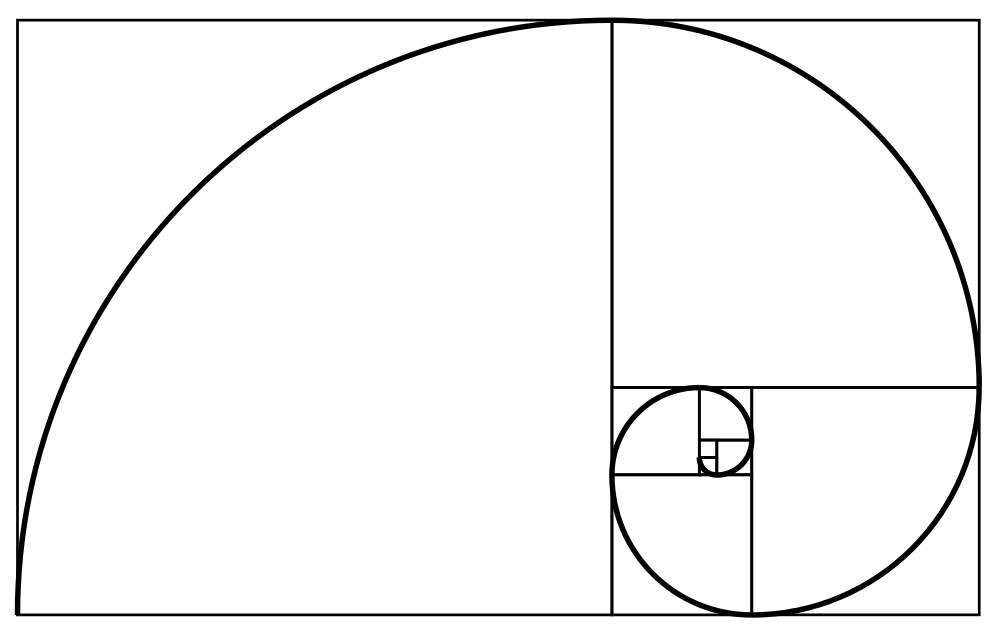
\includegraphics{img/fibonacci-spiral.eps}}
            }

\author{刘新宇
  \thanks{{\bfseries 刘新宇} \newline
    Version: 0.6180339887498949 \newline
    Email: liuxinyu95@gmail.com \newline
    }}

\maketitle

% ================================================================
%                 Content
% ================================================================

%\newpage
\tableofcontents
\newpage

\part{前言}
\ifx\wholebook\relax \else
% ------------------------

% \documentclass[UTF8]{ctexart}
\documentclass[UTF8]{article}

%%
% loading packages
%
\newif\ifpdf
\ifx\pdfoutput\undefined % We're not running pdftex
  \pdffalse
\else
  \pdftrue
\fi
%
%
\ifpdf
  \RequirePackage[pdftex,%
            CJKbookmarks,%
       bookmarksnumbered,%
              colorlinks,%
          linkcolor=blue,%
              hyperindex,%
        plainpages=false,%
       pdfstartview=FitH]{hyperref}
\else
  \RequirePackage[dvipdfm,%
             CJKbookmarks,%
        bookmarksnumbered,%
               colorlinks,%
           linkcolor=blue,%
               hyperindex,%
         plainpages=false,%
        pdfstartview=FitH]{hyperref}
  \AtBeginDvi{\special{pdf:tounicode GBK-EUC-UCS2}} % GBK -> Unicode
\fi
\usepackage{hyperref}

% other packages
%-----------------------------------------------------------------------------
\usepackage{graphicx, color}
\usepackage{CJK}
%
% for programming 
%
\usepackage{verbatim}
\usepackage{listings}


\lstdefinelanguage{Smalltalk}{
  morekeywords={self,super,true,false,nil,thisContext}, % This is overkill
  morestring=[d]',
  morecomment=[s]{"}{"},
  alsoletter={\#:},
  escapechar={!},
  literate=
    {BANG}{!}1
    {UNDERSCORE}{\_}1
    {\\st}{Smalltalk}9 % convenience -- in case \st occurs in code
    % {'}{{\textquotesingle}}1 % replaced by upquote=true in \lstset
    {_}{{$\leftarrow$}}1
    {>>>}{{\sep}}1
    {^}{{$\uparrow$}}1
    {~}{{$\sim$}}1
    {-}{{\sf -\hspace{-0.13em}-}}1  % the goal is to make - the same width as +
    %{+}{\raisebox{0.08ex}{+}}1		% and to raise + off the baseline to match -
    {-->}{{\quad$\longrightarrow$\quad}}3
	, % Don't forget the comma at the end!
  tabsize=2
}[keywords,comments,strings]

\lstloadlanguages{C++, Lisp, Smalltalk}

% ======================================================================

\def\BibTeX{{\rm B\kern-.05em{\sc i\kern-.025em b}\kern-.08em
    T\kern-.1667em\lower.7ex\hbox{E}\kern-.125emX}}

\newtheorem{theorem}{Theorem}

%
% mathematics
%
\newcommand{\be}{\begin{equation}}
\newcommand{\ee}{\end{equation}}
\newcommand{\bmat}[1]{\left( \begin{array}{#1} }
\newcommand{\emat}{\end{array} \right) }
\newcommand{\VEC}[1]{\mbox{\boldmath $#1$}}

% numbered equation array
\newcommand{\bea}{\begin{eqnarray}}
\newcommand{\eea}{\end{eqnarray}}

% equation array not numbered
\newcommand{\bean}{\begin{eqnarray*}}
\newcommand{\eean}{\end{eqnarray*}}

\RequirePackage{CJK,CJKnumb,CJKulem,CJKpunct}
% we use CJK as default environment
\AtBeginDocument{\begin{CJK*}{GBK}{song}\CJKtilde\CJKindent\CJKcaption{GB}}
\AtEndDocument{\clearpage\end{CJK*}}

%
% loading packages
%

\RequirePackage{ifpdf}
\RequirePackage{ifxetex}

%
%
\ifpdf
  \RequirePackage[pdftex,%
       bookmarksnumbered,%
              colorlinks,%
          linkcolor=blue,%
              hyperindex,%
        plainpages=false,%
       pdfstartview=FitH]{hyperref}
\else\ifxetex
  \RequirePackage[bookmarksnumbered,%
               colorlinks,%
           linkcolor=blue,%
               hyperindex,%
         plainpages=false,%
        pdfstartview=FitH]{hyperref}
\else
  \RequirePackage[dvipdfm,%
        bookmarksnumbered,%
               colorlinks,%
           linkcolor=blue,%
               hyperindex,%
         plainpages=false,%
        pdfstartview=FitH]{hyperref}
\fi\fi
%\usepackage{hyperref}

% other packages
%--------------------------------------------------------------------------
\usepackage{graphicx, color}
\usepackage{subfig}
\usepackage{tikz}
\usetikzlibrary{matrix,positioning}

\usepackage{amsmath, amsthm, amssymb} % for math
\usepackage{exercise} % for exercise
\usepackage{import} % for nested input

%
% for programming
%
\usepackage{verbatim}
\usepackage{listings}
%\usepackage{algorithmic} %old version; we can use algorithmicx instead
\usepackage{algorithm}
\usepackage[noend]{algpseudocode} %for pseudo code, include algorithmicsx automatically
\usepackage{appendix}
\usepackage{makeidx} % for index support
\usepackage{titlesec}

\usepackage[cm-default]{fontspec}
\usepackage{xunicode}

% detect and select Chinese font
% ------------------------------
% the following cmd can list all availabe Chinese fonts in host.
% fc-list :lang=zh
\def\myfont{STHeiti}  % Under Mac OS X
\def\linuxfallback{WenQuanYi Micro Hei} % Under Linux
\def\winfallback{SimSun} % Under Windows
\suppressfontnotfounderror1 % Avoid setting exit code (error level) to break make process
\count255=\interactionmode
\batchmode
\font\foo="\myfont"\space at 10pt
\ifx\foo\nullfont
  \font\foo = "\linuxfallback"\space at 10pt
  \ifx\foo\nullfont
    \font\foo = "\winfallback"\space at 10pt
    \ifx\foo\nullfont
      \errorstopmode
      \errmessage{no suitable Chinese font found}
    \else
      \let\myfont=\winfallback % Windows
    \fi
  \else
    \let\myfont=\linuxfallback % Linux
  \fi
\fi
\interactionmode=\count255
\setmainfont[Mapping=tex-text]{\myfont}

\XeTeXlinebreaklocale "zh"  % to solve the line breaking issue
\XeTeXlinebreakskip = 0pt plus 1pt minus 0.1pt

\titleformat{\paragraph}
{\normalfont\normalsize\bfseries}{\theparagraph}{1em}{}
\titlespacing*{\paragraph}
{0pt}{3.25ex plus 1ex minus .2ex}{1.5ex plus .2ex}

\lstdefinelanguage{Smalltalk}{
  morekeywords={self,super,true,false,nil,thisContext}, % This is overkill
  morestring=[d]',
  morecomment=[s]{"}{"},
  alsoletter={\#:},
  escapechar={!},
  literate=
    {BANG}{!}1
    {UNDERSCORE}{\_}1
    {\\st}{Smalltalk}9 % convenience -- in case \st occurs in code
    % {'}{{\textquotesingle}}1 % replaced by upquote=true in \lstset
    {_}{{$\leftarrow$}}1
    {>>>}{{\sep}}1
    {^}{{$\uparrow$}}1
    {~}{{$\sim$}}1
    {-}{{\sf -\hspace{-0.13em}-}}1  % the goal is to make - the same width as +
    %{+}{\raisebox{0.08ex}{+}}1		% and to raise + off the baseline to match -
    {-->}{{\quad$\longrightarrow$\quad}}3
	, % Don't forget the comma at the end!
  tabsize=2
}[keywords,comments,strings]

% for better Haskell code outlook
\lstdefinelanguage{Haskell}{
  basicstyle=\small\ttfamily,
  flexiblecolumns=false,
  basewidth={0.5em,0.45em},
  literate={+}{{$+$}}1 {/}{{$/$}}1 {*}{{$*$}}1 {=}{{$=$}}1
           {>}{{$>$}}1 {<}{{$<$}}1 {\\}{{$\lambda$}}1
           {\\\\}{{\char`\\\char`\\}}1
           {->}{{$\rightarrow$}}2 {>=}{{$\geq$}}2 {<-}{{$\leftarrow$}}2
           {<=}{{$\leq$}}2 {=>}{{$\Rightarrow$}}2
           {\ .}{{$\circ$}}2 {\ .\ }{{$\circ$}}2
           {>>}{{>>}}2 {>>=}{{>>=}}2
           {|}{{$\mid$}}1
}[keywords,comments,strings]

\lstloadlanguages{C, C++, Lisp, Haskell, Python, Smalltalk}

\lstset{
  showstringspaces = false
}

% ======================================================================

\def\BibTeX{{\rm B\kern-.05em{\sc i\kern-.025em b}\kern-.08em
    T\kern-.1667em\lower.7ex\hbox{E}\kern-.125emX}}

%
% mathematics
%
\newcommand{\be}{\begin{equation}}
\newcommand{\ee}{\end{equation}}
\newcommand{\bmat}[1]{\left( \begin{array}{#1} }
\newcommand{\emat}{\end{array} \right) }
\newcommand{\VEC}[1]{\mbox{\boldmath $#1$}}

% numbered equation array
\newcommand{\bea}{\begin{eqnarray}}
\newcommand{\eea}{\end{eqnarray}}

% equation array not numbered
\newcommand{\bean}{\begin{eqnarray*}}
\newcommand{\eean}{\end{eqnarray*}}

\newtheorem{theorem}{Theorem}[section]
\newtheorem{lemma}[theorem]{Lemma}
\newtheorem{proposition}[theorem]{Proposition}
\newtheorem{corollary}[theorem]{Corollary}


\setcounter{page}{1}

\begin{document}

%--------------------------

% ================================================================
%                 COVER PAGE
% ================================================================

\title{前言}

\author{刘新宇
\thanks{{\bfseries 刘新宇} \newline
  Email: liuxinyu95@gmail.com \newline}
  }

\maketitle
\fi

\markboth{前言}{初等算法}

% ================================================================
%                 Why
% ================================================================
\section{Why?}
\label{why}

“算法有用么?”经常有人问我这个问题。很多人在工作中根本不用算法。偶尔碰到的时候,也不过是使用一些实现好的库。例如C++标准模版库STL中有现成的排序、查找函数;常用的数据结构如向量(vector)、队列(queue)、集合(set)也都实现好了。日常工作中了解如何使用这些库似乎就足够了。

算法在解决一些“有趣”的问题时,会扮演关键角色。但是这些问题本身的价值,却是仁者见仁、智者见智。

让我们用例子来说话吧。下面两道题目,即使是初学编程的新手,似乎也很容易解决。

% ================================================================
%      Mininum free ID problem. The power of algorithms
% ================================================================
\section{最小可用ID,算法的威力}
\label{min-free} \index{minimum free number}

这道题目来自Richard Bird书中的第一章\cite{Bird-book}。现代社会中,有很多服务依赖一种被称为ID的概念。例如身份证就是一种ID,银行账户也是一种ID,电话号码本质上也是一种ID。假设我们使用非负整数作为某个系统的的ID,所有用户都由一个ID唯一确定。任何时间,这个系统中有些ID处在使用中的状态,有些ID则可以用于分配给新用户。现在的问题是,怎样才能找到最小的可用ID呢?例如下面的列表记录了当前正在被使用的ID:

\begin{verbatim}
[18, 4, 8, 9, 16, 1, 14, 7, 19, 3, 0, 5, 2, 11, 6]
\end{verbatim}

最小可用的ID,也就是不在这个列表中的最小整数是10。这个题目看上去是如此简单,我们可以立即写出下面解法:

\begin{algorithmic}[1]
\Function{Min-Free}{$A$}
  \State $x \gets 0$
  \Loop
    \If{$x \notin A$}
      \State \Return $x$
    \Else
      \State $x \gets x + 1$
    \EndIf
  \EndLoop
\EndFunction
\end{algorithmic}

其中符号$\notin$的实现如下:

\begin{algorithmic}[1]
\Function{`$\notin$'}{$x, X$}
  \For{$i \gets 1 $ to $|X|$}
    \If{$x = X[i]$}
      \State \Return False
    \EndIf
  \EndFor
  \State \Return True
\EndFunction
\end{algorithmic}

有些编程语言内置了这一线性查找的实现。例如我们可以直接将这一解法翻译成下面的Python程序。

\lstset{language=Python}
\begin{lstlisting}
def brute_force(lst):
    i = 0
    while True:
        if i not in lst:
            return i
        i = i + 1
\end{lstlisting}

但是这道题目仅仅是看上去简单。在一个存储了几百万个ID的大型系统中,这个方法的的性能很差。对于一个长度为n的ID列表,它需要$O(n^2)$的时间才能找到最小可用的ID。在我的计算机上(双核2.10GHz处理器,2G内存),使用这一方法的C语言程序平均需要约5.4秒才能在十万个ID中找到答案\footnote{所有代码均可随本书一起下载}。当ID的数量上升到一百万时,平均用时则长达8分钟。

\subsection{改进一}
改进这一解法的关键基于这一事实:对于任何$n$个非负整数$x_1, x_2, ..., x_n$,如果存在小于$n$的可用整数,必然存在某个$x_i$不在$[0, n)$这个范围内。否则这些整数一定是$0, 1, ..., n-1$的某个排列,这种情况下,最小的可用整数是$n$。于是我们有如下结论:

\be
minfree(x_1, x_2, ..., x_n) \leq n
\label{min-free}
\ee

根据这一结论,我们可以用一个长度为$n+1$的数组,来标记区间$[0, n]$内的某个整数是否可用。

\begin{algorithmic}[1]
\Function{Min-Free}{$A$}
  \State $F \gets [False, False, ..., False]$ where $|F| = n+1$
  \For{$\forall x \in A$}
    \If{$x < n$}
      \State $F[x] \gets$ True
    \EndIf
  \EndFor
  \For{$i \gets [0, n]$}
    \If{$F[i] =$ False}
      \State \Return $i$
    \EndIf
  \EndFor
\EndFunction
\end{algorithmic}

其中第2行将标志数组中的所有值初始化为False,这一步骤需要$O(n)$的时间。接着我们遍历$A$中的所有元素,只要小于$n$,就将相应的标记置为True。这一过程也需要$O(n)$的时间。最后我们再线性查找标志数组中第一个值为Fasle的位置。整个算法的性能是线性时间$O(n)$的。注意,我们使用了$n+1$个标志,而不是$n$个标志。这样无需额外处理,就可以应对$sorted(A) = [0, 1, 2, ..., n-1]$
的特殊情况。

虽然这个方法只需要线性时间,但是它需要使用$O(n)$的空间来存储标志。

这一方法比之前的暴力解法快很多。在我的计算机上,相应的Python程序平均只用0.02秒,就可以在十万个整数中找到答案。

我们还可以继续优化。每次查找,我们都需要申请长度为$n+1$的数组;查找结束后,这个数组又被释放掉了。反复的申请和释放会占用不少时间。我们可以预先准备好足够长的数组,然后每次查找都复用它。另外,我们可以使用二进制的位来保存标志,这样能节约不少空间。下面的C语言程序实现了这两点小改进。

\lstset{language = C}
\begin{lstlisting}
#define N 1000000 // 1 million
#define WORD_LENGTH sizeof(int) * 8

void setbit(unsigned int* bits, unsigned int i){
  bits[i / WORD_LENGTH] |= 1<<(i % WORD_LENGTH);
}

int testbit(unsigned int* bits, unsigned int i){
  return bits[i/WORD_LENGTH] & (1<<(i % WORD_LENGTH));
}

unsigned int bits[N/WORD_LENGTH+1];

int min_free(int* xs, int n){
  int i, len = N/WORD_LENGTH+1;
  for(i=0; i<len; ++i)
    bits[i]=0;
  for(i=0; i<n; ++i)
    if(xs[i]<n)
      setbit(bits, xs[i]);
  for(i=0; i<=n; ++i)
    if(!testbit(bits, i))
      return i;
}
\end{lstlisting}

在我的计算机上,这段C程序处理一百万个整数,平均用时仅仅0.023秒。最后一个for循环还能
进一步改进如下,但这些都是一些微调了。

\begin{lstlisting}
  for(i=0; ; ++i)
    if(~bits[i] !=0 )
      for(j=0; ; ++j)
	if(!testbit(bits, i*WORD_LENGTH+j))
	  return i*WORD_LENGTH+j;
\end{lstlisting}

\subsection{改进二、分而治之}
我们在速度上的改进是以空间上的消耗为代价的。由于维护了一个长度为$n$的标志数组,当$n$很大时,空间上的性能就成了新的瓶颈。

分而治之的典型策略是将问题分解为若干较小规模的子问题,然后逐步解决这些子问题以得到最终的结果。

我们可以将所有满足$x_i \leq \lfloor n/2 \rfloor$的整数放入一个子序列$A'$;将剩余的其他整数放入另外一个序列$A''$。根据公式\ref{min-free},如果序列$A'$的长度正好是$\lfloor n/2 \rfloor$,这说明前一半的整数已经“满了”,最小的可用整数一定可以在$A''$中递归地找到。否则,最小的可用整数可以在$A'$中找到。总之,通过这一划分,问题的规模减小了。

需要注意的是,当我们在子序列$A''$中递归查找时,边界情况发生了一些变化,我们不再是从0开始寻找最小可用整数,查找的下界变成了$\lfloor n/2 \rfloor + 1$。因此我们的算法应定义为$minfree(A, l, u)$,其中$l$和$u$分别是上下界。

递归结束的边界条件是当待查找的序列变为空的时候,此时我们只需要返回下界作为结果即可。

根据上述思路,分而治之的解法可以形式化地定义为一个函数:

\[
minfree(A) = search(A, 0, |A|-1)
\]

\[
search(A, l, u) = \left \{
       \begin{array}
       {r@{\quad:\quad}l}
       l & A = \phi \\
       search(A'', m+1, u) &  |A'| = m - l + 1 \\
       search(A',  l, m) & otherwise
       \end{array}
\right.
\]

其中

\[ \begin{array}{l}
m = \displaystyle \lfloor \frac{l+u}{2} \rfloor \\
A'  = \{ \forall x \in A \wedge x \leq m \} \\
A'' = \{ \forall x \in A \wedge x > m \} \\
\end{array} \]

It is obvious that this algorithm doesn't need any extra
space\footnote{Procedural programmer may note that it
actually takes $O(\lg n)$ stack spaces for book-keeping. As
we'll see later, this can be eliminated either by tail
recursion optimization, for instance gcc -O2. or by manually
changing the recursion to iteration}. Each call
performs $O(|A|)$ comparison to build $A'$ and $A''$.
After that the problem scale halves.
So the time needed for this algorithm is $T(n) = T(n/2) + O(n)$
which reduce to $O(n)$. Another way to analyze the performance
is by observing that the first call takes $O(n)$
to build $A'$ and $A''$ and the second call takes
$O(n/2)$, and $O(n/4)$ for the third... The total
time is $O(n + n/2 + n/4 + ...) = O(2n) = O(n)$ .

In functional programming languages such as Haskell,
partitioning a list has already been provided in the basic library
and this algorithm can be translated as the following.

\lstset{language=Haskell}
\begin{lstlisting}
import Data.List

minFree xs = bsearch xs 0 (length xs - 1)

bsearch xs l u | xs == [] = l
               | length as == m - l + 1 = bsearch bs (m+1) u
               | otherwise = bsearch as l m
    where
      m = (l + u) `div` 2
      (as, bs) = partition (<=m) xs
\end{lstlisting}

\subsection{Expressiveness vs. Performance}
Imperative language programmers may be concerned about the performance
of this kind of implementation. For instance in this minimum
free ID problem, the number of recursive calls is in $O(\lg n)$
, which means the stack size consumed is in $O(\lg n)$.
It's not free in terms of space. But if we want to avoid that
, we can eliminate the recursion by replacing it by an iteration
\footnote{This is done automatically in most functional languages
since our function is in tail recursive form which lends itself
perfectly to this transformation} which yields the following C program.

\lstset{language=C}
\begin{lstlisting}
int min_free(int* xs, int n){
  int l=0;
  int u=n-1;
  while(n){
    int m = (l + u) / 2;
    int right, left = 0;
    for(right = 0; right < n; ++ right)
      if(xs[right] <= m){
	swap(xs[left], xs[right]);
	++left;
      }
    if(left == m - l + 1){
      xs = xs + left;
      n  = n - left;
      l  = m+1;
    }
    else{
      n = left;
      u = m;
    }
  }
  return l;
}
\end{lstlisting}

This program uses a `quick-sort' like approach to re-arrange the
array so that all the elements before $left$ are less than or equal
to $m$; while those between $left$ and $right$ are greater
than $m$. This is shown in figure \ref{fig:divide}.

\begin{figure}[htbp]
  \centering
  \includegraphics[scale=1]{img/divide-by-m.ps}
  \caption{Divide the array, all $x[i] \leq m$ where $0 \leq i < left$; while all $x[i] > m$ where $left \leq i < right$. The left elements are unknown.} \label{fig:divide}
\end{figure}

This program is fast and it doesn't need extra stack space. However,
compared to the previous Haskell program, it's hard to read and the
expressiveness decreased. We have to balance performance
and expressiveness.

\section{The number puzzle, power of data structure}

If the first problem, to find the minimum free number, is a some what
useful in practice, this problem is a `pure' one for fun. The puzzle
is to find the 1,500th number, which only contains factor 2, 3 or 5.
The first 3 numbers are of course 2, 3, and 5. Number $60 = 2^23^15^1$,
However it is the 25th number. Number $21 = 2^03^17^1$, isn't a valid
number because it contains a factor 7. The first 10 such numbers are list
as the following.

2,3,4,5,6,8,9,10,12,15

If we consider $1=2^03^05^0$, then 1 is also a valid number and it is
the first one.

\subsection{The brute-force solution}
It seems the solution is quite easy without need any serious algorithms.
We can check all numbers from 1, then extract all factors of 2, 3 and 5
to see if the left part is 1.

\begin{algorithmic}[1]
\Function{Get-Number}{$n$}
  \State $x \gets 1$
  \State $i \gets 0$
  \Loop
    \If{\Call{Valid?}{$x$}}
      \State $i \gets i + 1$
      \If{$i = n$}
        \State \Return $x$
      \EndIf
    \EndIf
    \State $x \gets x + 1$
  \EndLoop
\EndFunction
\Statex
\Function{Valid?}{$x$}
  \While{$x \bmod 2 = 0$}
    \State $x \gets x / 2$
  \EndWhile
  \While{$x \bmod 3 = 0$}
    \State $x \gets x / 3$
  \EndWhile
  \While{$x \bmod 5 = 0$}
    \State $x \gets x / 5$
  \EndWhile
  \If{$x = 1$}
    \State \Return $True$
  \Else
    \State \Return $False$
  \EndIf
\EndFunction
\end{algorithmic}

This `brute-force' algorithm works for most small $n$. However, to find
the 1500th number (which is 859963392), the C program based on this
algorithm takes 40.39 seconds in my computer. I have to kill the program
after 10 minutes when I increased $n$ to 15,000.

\subsection{Improvement 1}
Analysis of the above algorithm shows that modular and divide calculations
are very expensive \cite{Bentley}. And they executed a lot in loops.
Instead of checking a number contains only 2, 3, or 5 as factors, one
alternative solution is to construct such number by these factors.

We start from 1, and times it with 2, or 3, or 5 to generate rest numbers.
The problem turns to be how to generate the candidate number in order?
One handy way is to utilize the queue data structure.

A queue data structure is used to push elements at one end, and pops
them at the other end. So that the element be pushed first is also
be popped out first. This property is called FIFO (First-In-First-Out).

The idea is to push 1 as the only element to the queue, then we pop
an element, times it with 2, 3, and 5, to get 3 new elements. We
then push them back to the queue in order. Note that, the new elements may
have already existed in the queue. In such case, we just drop the
element. The new element may also smaller than the others in the queue,
so we must put them to the correct position. Figure \ref{fig:queues}
illustrates this idea.

\begin{figure}[htbp]
       \begin{center}
       	  \includegraphics[scale=0.5]{img/q1.ps}
       	  \includegraphics[scale=0.5]{img/q2.ps}
       	  \includegraphics[scale=0.5]{img/q3.ps}
       	  \includegraphics[scale=0.5]{img/q4.ps}
        \caption{First 4 steps of constructing numbers with a queue. \newline
        1. Queue is initialized with 1 as the only element;\newline
        2. New elements 2, 3, and 5 are pushed back; \newline
        3. New elements 4, 6, and 10, are pushed back in order; \newline
        4. New elements 9 and 15 are pushed back, element 6 already exists.} \label{fig:queues}
       \end{center}
\end{figure}

This algorithm is shown as the following.

\begin{algorithmic}[1]
\Function{Get-Number}{$n$}
  \State $Q \gets NIL$
  \State \Call{Enqueue}{$Q, 1$}
  \While{$n > 0$}
    \State $x \gets$ \Call{Dequeue}{$Q$}
    \State \Call{Unique-Enqueue}{$Q, 2x$}
    \State \Call{Unique-Enqueue}{$Q, 3x$}
    \State \Call{Unique-Enqueue}{$Q, 5x$}
    \State $n \gets n-1$
  \EndWhile
  \State \Return $x$
\EndFunction
\Statex
\Function{Unique-Enqueue}{$Q, x$}
  \State $i \gets 0$
  \While{$i < |Q| \wedge Q[i] < x$}
    \State $i \gets i + 1$
  \EndWhile
  \If{$i < |Q| \wedge x = Q[i]$}
    \State \Return
  \EndIf
  \State \Call{Insert}{$Q, i, x$}
\EndFunction
\end{algorithmic}

The insert function takes $O(|Q|)$ time to find the proper position and insert
it. If the element has already existed, it just returns.

A rough estimation tells that the length of the queue increase proportion to $n$,
(Each time, we extract one element, and pushed 3 new, the increase ratio $\leq$ 2),
so the total running time is $O(1+2+3+...+n) = O(n^2)$.

Figure\ref{fig:big-O-1q} shows the number of queue access time against $n$.
It is quadratic curve which reflect the $O(n^2)$ performance.

\begin{figure}[htbp]
       \begin{center}
       	  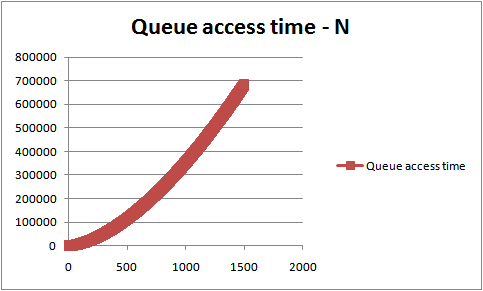
\includegraphics[scale=0.5]{img/big-O-1q.eps}
        \caption{Queue access count v.s. $n$.} \label{fig:big-O-1q}
       \end{center}
\end{figure}

The C program based on this algorithm takes only 0.016[s] to get the right answer
859963392. Which is 2500 times faster than the brute force solution.

%% Functional 1Q solution
Improvement 1 can also be considered in recursive way. Suppose $X$ is the infinity
series for all numbers which only contain factors of 2, 3, or 5. The following
formula shows an interesting relationship.

\be
  X = \{1\} \cup \{2x: \forall x \in X\} \cup \{3x: \forall x \in X \} \cup \{5x: \forall x \in X \}
\ee

Where we can define $\cup$ to a special form so that all elements are stored in order
as well as unique to each other. Suppose that $X=\{x_1, x_2, x_3...\}$, $Y=\{y_1, y_2, y_3, ...\}$, $X' = \{x_2, x_3, ...\}$ and $Y'=\{y_2, y_3, ...\}$. We have

\[
X \cup Y = \left \{
  \begin{array}{r@{\quad:\quad}l}
  X & Y = \phi \\
  Y & X = \phi \\
  \{ x_1, X' \cup Y \} & x_1 < y_1 \\
  \{ x_1, X' \cup Y' \} & x_1 = y_1 \\
  \{ y_1, X \cup Y' \} & x_1 > y_1
  \end{array}
\right.
\]

In a functional programming language such as Haskell, which supports
lazy evaluation, The above infinity series functions can be translate
into the following program.

\lstset{language=Haskell}
\begin{lstlisting}
ns = 1:merge (map (*2) ns) (merge (map (*3) ns) (map (*5) ns))

merge [] l = l
merge l [] = l
merge (x:xs) (y:ys) | x <y = x : merge xs (y:ys)
                    | x ==y = x : merge xs ys
                    | otherwise = y : merge (x:xs) ys
\end{lstlisting}

By evaluate ns !! (n-1), we can get the 1500th number as
below.

\begin{verbatim}
>ns !! (1500-1)
859963392
\end{verbatim}

\subsection{Improvement 2}
Considering the above solution, although it is much faster than the brute-force one,
It still has some drawbacks. It produces many duplicated numbers and they are
finally dropped when examine the queue. Secondly, it does linear scan and insertion
to keep the order of all elements in the queue, which degrade the ENQUEUE operation
from $O(1)$ to $O(|Q|)$.

If we use three queues instead of using only one, we can improve the solution one
step ahead. Denote these queues as $Q_2$, $Q_3$, and $Q_5$, and we initialize
them as $Q_2=\{ 2 \}$, $Q_3 = \{ 3\}$ and $Q_5 = \{ 5 \}$. Each time we DEQUEUEed
the smallest one from $Q_2$, $Q_3$, and $Q_5$ as $x$. And do the following test:

\begin{itemize}
\item If $x$ comes from $Q_2$, we ENQUEUE $2x$, $3x$, and $5x$ back to
$Q_2$, $Q_3$, and $Q_5$ respectively;
\item If $x$ comes from $Q_3$, we only need ENQUEUE $3x$ to $Q_3$, and $5x$ to $Q_5$;
We needn't ENQUEUE $2x$ to $Q_2$, because $2x$ have already existed in $Q_3$;
\item If $x$ comes from $Q_5$, we only need ENQUEUE $5x$ to $Q_5$; there is
no need to ENQUEUE $3x$, $5x$ to $Q_3$, $Q_5$ because they have already been
in the queues;
\end{itemize}

We repeatedly ENQUEUE the smallest one until we find the $n$-th element.

\begin{figure}[htbp]
       \begin{center}
       	  \includegraphics[scale=0.5]{img/q235-1.ps}
       	  \includegraphics[scale=0.5]{img/q235-2.ps}
       	  \includegraphics[scale=0.5]{img/q235-3.ps}
       	  \includegraphics[scale=0.5]{img/q235-4.ps}
        \caption{First 4 steps of constructing numbers with $Q_2$, $Q_3$, and $Q_5$. \newline
        1. Queues are initialized with 2, 3, 5 as the only element;\newline
        2. New elements 4, 6, and 10 are pushed back; \newline
        3. New elements 9, and 15, are pushed back; \newline
        4. New elements 8, 12, and 20 are pushed back; \newline
        5. New element 25 is pushed back.} \label{fig:q235}
       \end{center}
\end{figure}

The algorithm based on this idea is implemented as below.

\begin{algorithmic}[1]
\Function{Get-Number}{$n$}
  \If{$n = 1$}
    \State \Return $1$
  \Else
    \State $Q_2 \gets \{ 2 \}$
    \State $Q_3 \gets \{ 3 \}$
    \State $Q_5 \gets \{ 5 \}$
    \While{$n > 1$}
      \State $x \gets min($\Call{Head}{$Q_2$}, \Call{Head}{$Q_3$}, \Call{Head}{$Q_5$}$)$
      \If{$x = $ \Call{Head}{$Q_2$}}
        \State \Call{Dequeue}{$Q_2$}
        \State \Call{Enqueue}{$Q_2, 2x$}
        \State \Call{Enqueue}{$Q_3, 3x$}
        \State \Call{Enqueue}{$Q_5, 5x$}
      \ElsIf{$x=$ \Call{Head}{$Q_3$}}
        \State \Call{Dequeue}{$Q_3$}
        \State \Call{Enqueue}{$Q_3, 3x$}
        \State \Call{Enqueue}{$Q_5, 5x$}
      \Else
        \State \Call{Dequeue}{$Q_5$}
        \State \Call{Enqueue}{$Q_5, 5x$}
      \EndIf
      \State $n \gets n - 1$
    \EndWhile
    \State \Return $x$
  \EndIf
\EndFunction
\end{algorithmic}

This algorithm loops $n$ times, and within each loop, it extract one head
element from the three queues, which takes constant time. Then it appends
one to three new elements at the end of queues which bounds to constant time
too. So the total time of the algorithm bounds to $O(n)$. The C++ program
translated from this algorithm shown below takes less than 1 $\mu$s to
produce the 1500th number, 859963392.

\lstset{language=C++}
\begin{lstlisting}
typedef unsigned long Integer;

Integer get_number(int n){
  if(n==1)
    return 1;
  queue<Integer> Q2, Q3, Q5;
  Q2.push(2);
  Q3.push(3);
  Q5.push(5);
  Integer x;
  while(n-- > 1){
    x = min(min(Q2.front(), Q3.front()), Q5.front());
    if(x==Q2.front()){
      Q2.pop();
      Q2.push(x*2);
      Q3.push(x*3);
      Q5.push(x*5);
    }
    else if(x==Q3.front()){
      Q3.pop();
      Q3.push(x*3);
      Q5.push(x*5);
    }
    else{
      Q5.pop();
      Q5.push(x*5);
    }
  }
  return x;
}
\end{lstlisting}

This solution can be also implemented in Functional way. We define
a function $take(n)$, which will return the first $n$ numbers contains
only factor 2, 3, or 5.

\[
  take(n) = f(n, \{1\}, \{2\}, \{3\}, \{5\})
\]
Where
\[
 f(n, X, Q_2, Q_3, Q_5) = \left \{
  \begin{array}{r@{\quad:\quad}l}
  X & n = 1 \\
  f(n-1, X \cup \{x\}, Q_2', Q_3', Q_5') & otherwise
  \end{array}
\right.
\]

\[
 x = min(Q_{21}, Q_{31}, Q_{51})
\]
\[
 Q_2', Q_3', Q_5' = \left \{
 \begin{array}{r@{\quad:\quad}l}
 \{Q_{22}, Q_{23}, ...\} \cup \{2x\}, Q_3 \cup \{3x\}, Q_5 \cup \{5x\} & x = Q_{21} \\
 Q_2, \{Q_{32}, Q_{33}, ...\} \cup \{3x\}, Q5 \cup \{5x\} & x = Q_{31} \\
 Q_2, Q_3, \{Q_{52}, Q_{53}, ...\} \cup \{5x\} & x = Q_{51}
 \end{array}
 \right.
\]

And these functional definition can be realized in Haskell as the following.

\lstset{language=Haskell}
\begin{lstlisting}
ks 1 xs _ = xs
ks n xs (q2, q3, q5) = ks (n-1) (xs++[x]) update
    where
      x = minimum $ map head [q2, q3, q5]
      update | x == head q2 = ((tail q2)++[x*2], q3++[x*3], q5++[x*5])
             | x == head q3 = (q2, (tail q3)++[x*3], q5++[x*5])
             | otherwise = (q2, q3, (tail q5)++[x*5])

takeN n = ks n [1] ([2], [3], [5])
\end{lstlisting} %$

Invoke `last takeN 1500' will generate the correct answer 859963392.

% ================================================================
%                 Short summary
% ================================================================
\section{Notes and short summary}
If review the 2 puzzles, we found in both cases, the brute-force solutions
are so weak. In the first problem, it's quite poor in dealing with
long ID list, while in the second problem, it doesn't work at all.

The first problem shows the power of algorithms, while the second
problem tells why data structure is important. There are plenty
of interesting problems, which are hard to solve before computer
was invented. With the aid of computer and programming, we are able
to find the answer in a quite different way. Compare to what we
learned in mathematics course in school, we haven't been taught the method
like this.

While there have been already a lot of wonderful books about
algorithms, data structures and math, however, few of them
provide the comparison between the procedural solution and
the functional solution. From the above discussion, it can be
found that functional solution sometimes is very expressive
and they are close to what we are familiar in mathematics.

This series of post focus on providing both imperative and functional
algorithms and data structures. Many functional data structures
can be referenced from Okasaki's book\cite{okasaki-book}. While
the imperative ones can be founded in classic text books \cite{CLRS}
or even in WIKIpedia.
Multiple
programming languages, including, C, C++, Python, Haskell, and
Scheme/Lisp will be used. In order to make it easy to read
by programmers with different background, pseudo code and mathematical
function are the regular descriptions of each post.

The author is NOT a native English speaker, the reason why
this book is only available in English for the time being
is because the contents are still changing frequently. Any
feedback, comments, or criticizes are welcome.

\section{Structure of the contents}
In the following series of post, I'll first introduce about
elementary data structures before algorithms, because many
algorithms need knowledge of data structures as prerequisite.

The `hello world' data structure, binary search tree is the
first topic; Then we introduce how to solve the balance problem
of binary search tree. After that, I'll show other interesting
trees. Trie, Patricia, suffix trees are useful in text manipulation.
While B-trees are commonly used in file system and data base
implementation.

The second part of data structures is about heaps. We'll
provide a general Heap definition and introduce about binary
heaps by array and by explicit binary trees. Then we'll
extend to K-ary heaps including Binomial heaps, Fibonacci
heaps, and pairing heaps.

Array and queues are considered among the easiest data structures
typically, However, we'll show how difficult to implement
them in the third part.

As the elementary sort algorithms, we'll introduce insertion
sort, quick sort, merge sort etc in both imperative way
and functional way.

The final part is about searching, besides the element
searching, we'll also show string matching algorithms
such as KMP.

All the posts are provided under GNU FDL (Free document
license), and programs are under GNU GPL.

% ================================================================
%                 Appendix
% ================================================================
\section{Appendix} \label{appendix}
%\appendix
All programs provided along with this book are free for
downloading. download position:
  http://sites.google.com/site/algoxy/home

\begin{thebibliography}{99}

\bibitem{Bird-book}
Richard Bird. ``Pearls of functional algorithm design''. Cambridge University Press; 1 edition (November 1, 2010). ISBN-10: 0521513383

\bibitem{Bentley}
Jon Bentley. ``Programming Pearls(2nd Edition)''. Addison-Wesley Professional; 2 edition (October 7, 1999). ISBN-13: 978-0201657883

\bibitem{okasaki-book}
Chris Okasaki. ``Purely Functional Data Structures''. Cambridge university press, (July 1, 1999), ISBN-13: 978-0521663502

\bibitem{CLRS}
Thomas H. Cormen, Charles E. Leiserson, Ronald L. Rivest and Clifford Stein. ``Introduction to Algorithms, Second Edition''. The MIT Press, 2001. ISBN: 0262032937.

\end{thebibliography}

\ifx\wholebook\relax \else
\end{document}
\fi


\part{树}
\ifx\wholebook\relax \else
% ------------------------

\documentclass[UTF8]{article}
%
% loading packages
%

\RequirePackage{ifpdf}
\RequirePackage{ifxetex}

%
%
\ifpdf
  \RequirePackage[pdftex,%
       bookmarksnumbered,%
              colorlinks,%
          linkcolor=blue,%
              hyperindex,%
        plainpages=false,%
       pdfstartview=FitH]{hyperref}
\else\ifxetex
  \RequirePackage[bookmarksnumbered,%
               colorlinks,%
           linkcolor=blue,%
               hyperindex,%
         plainpages=false,%
        pdfstartview=FitH]{hyperref}
\else
  \RequirePackage[dvipdfm,%
        bookmarksnumbered,%
               colorlinks,%
           linkcolor=blue,%
               hyperindex,%
         plainpages=false,%
        pdfstartview=FitH]{hyperref}
\fi\fi
%\usepackage{hyperref}

% other packages
%--------------------------------------------------------------------------
\usepackage{graphicx, color}
\usepackage{subfig}
\usepackage{tikz}
\usetikzlibrary{matrix,positioning}

\usepackage{amsmath, amsthm, amssymb} % for math
\usepackage{exercise} % for exercise
\usepackage{import} % for nested input

%
% for programming
%
\usepackage{verbatim}
\usepackage{listings}
%\usepackage{algorithmic} %old version; we can use algorithmicx instead
\usepackage{algorithm}
\usepackage[noend]{algpseudocode} %for pseudo code, include algorithmicsx automatically
\usepackage{appendix}
\usepackage{makeidx} % for index support
\usepackage{titlesec}

\usepackage[cm-default]{fontspec}
\usepackage{xunicode}

% detect and select Chinese font
% ------------------------------
% the following cmd can list all availabe Chinese fonts in host.
% fc-list :lang=zh
\def\myfont{STHeiti}  % Under Mac OS X
\def\linuxfallback{WenQuanYi Micro Hei} % Under Linux
\def\winfallback{SimSun} % Under Windows
\suppressfontnotfounderror1 % Avoid setting exit code (error level) to break make process
\count255=\interactionmode
\batchmode
\font\foo="\myfont"\space at 10pt
\ifx\foo\nullfont
  \font\foo = "\linuxfallback"\space at 10pt
  \ifx\foo\nullfont
    \font\foo = "\winfallback"\space at 10pt
    \ifx\foo\nullfont
      \errorstopmode
      \errmessage{no suitable Chinese font found}
    \else
      \let\myfont=\winfallback % Windows
    \fi
  \else
    \let\myfont=\linuxfallback % Linux
  \fi
\fi
\interactionmode=\count255
\setmainfont[Mapping=tex-text]{\myfont}

\XeTeXlinebreaklocale "zh"  % to solve the line breaking issue
\XeTeXlinebreakskip = 0pt plus 1pt minus 0.1pt

\titleformat{\paragraph}
{\normalfont\normalsize\bfseries}{\theparagraph}{1em}{}
\titlespacing*{\paragraph}
{0pt}{3.25ex plus 1ex minus .2ex}{1.5ex plus .2ex}

\lstdefinelanguage{Smalltalk}{
  morekeywords={self,super,true,false,nil,thisContext}, % This is overkill
  morestring=[d]',
  morecomment=[s]{"}{"},
  alsoletter={\#:},
  escapechar={!},
  literate=
    {BANG}{!}1
    {UNDERSCORE}{\_}1
    {\\st}{Smalltalk}9 % convenience -- in case \st occurs in code
    % {'}{{\textquotesingle}}1 % replaced by upquote=true in \lstset
    {_}{{$\leftarrow$}}1
    {>>>}{{\sep}}1
    {^}{{$\uparrow$}}1
    {~}{{$\sim$}}1
    {-}{{\sf -\hspace{-0.13em}-}}1  % the goal is to make - the same width as +
    %{+}{\raisebox{0.08ex}{+}}1		% and to raise + off the baseline to match -
    {-->}{{\quad$\longrightarrow$\quad}}3
	, % Don't forget the comma at the end!
  tabsize=2
}[keywords,comments,strings]

% for better Haskell code outlook
\lstdefinelanguage{Haskell}{
  basicstyle=\small\ttfamily,
  flexiblecolumns=false,
  basewidth={0.5em,0.45em},
  literate={+}{{$+$}}1 {/}{{$/$}}1 {*}{{$*$}}1 {=}{{$=$}}1
           {>}{{$>$}}1 {<}{{$<$}}1 {\\}{{$\lambda$}}1
           {\\\\}{{\char`\\\char`\\}}1
           {->}{{$\rightarrow$}}2 {>=}{{$\geq$}}2 {<-}{{$\leftarrow$}}2
           {<=}{{$\leq$}}2 {=>}{{$\Rightarrow$}}2
           {\ .}{{$\circ$}}2 {\ .\ }{{$\circ$}}2
           {>>}{{>>}}2 {>>=}{{>>=}}2
           {|}{{$\mid$}}1
}[keywords,comments,strings]

\lstloadlanguages{C, C++, Lisp, Haskell, Python, Smalltalk}

\lstset{
  showstringspaces = false
}

% ======================================================================

\def\BibTeX{{\rm B\kern-.05em{\sc i\kern-.025em b}\kern-.08em
    T\kern-.1667em\lower.7ex\hbox{E}\kern-.125emX}}

%
% mathematics
%
\newcommand{\be}{\begin{equation}}
\newcommand{\ee}{\end{equation}}
\newcommand{\bmat}[1]{\left( \begin{array}{#1} }
\newcommand{\emat}{\end{array} \right) }
\newcommand{\VEC}[1]{\mbox{\boldmath $#1$}}

% numbered equation array
\newcommand{\bea}{\begin{eqnarray}}
\newcommand{\eea}{\end{eqnarray}}

% equation array not numbered
\newcommand{\bean}{\begin{eqnarray*}}
\newcommand{\eean}{\end{eqnarray*}}

\newtheorem{theorem}{Theorem}[section]
\newtheorem{lemma}[theorem]{Lemma}
\newtheorem{proposition}[theorem]{Proposition}
\newtheorem{corollary}[theorem]{Corollary}


\setcounter{page}{1}

\begin{document}

%--------------------------

% ================================================================
%                 COVER PAGE
% ================================================================

\title{二叉搜索树,数据结构中的`hello world'}

\author{刘新宇
\thanks{{\bfseries 刘新宇} \newline
  Email: liuxinyu95@gmail.com \newline}
  }

\maketitle
\fi

\markboth{二叉搜索树}{初等算法}

\ifx\wholebook\relax
\chapter{二叉搜索树,数据结构中的`hello world'}
\numberwithin{Exercise}{chapter}
\fi

% ================================================================
%                 Introduction
% ================================================================
\section{简介}
\label{introduction} \index{二叉搜索树}

数组和链表通常被认为是最简单的“hello world”式数据结构。其实它们并不简单。在某些系统中,数组是最基本的数据结构,甚至链表也可以由数组来实现(《算法导论》第10.3节\cite{CLRS})。另一方面,在某些函数式环境中,链表被作为最基本的数据结构来实现数组和其他更复杂的数据结构。

考虑这些因素,我们使用二叉搜索树(BST)作为“hello world”数据结构。Jon Bentley在他的《编程珠玑》一书中,曾经给了这样一个有趣的题目\cite{Bentley}:如何统计一段文字中每个单词出现多少次?下面的C++程序展示了一个解法。\index{word counter}

\lstset{language=C++}
\begin{lstlisting}
int main(int, char** ){
  map<string, int> dict;
  string s;
  while(cin>>s)
    ++dict[s];
  map<string, int>::iterator it=dict.begin();
  for(; it!=dict.end(); ++it)
    cout<<it->first<<": "<<it->second<<"\n";
}
\end{lstlisting}

我们可以运行下面的UNIX命令获得对单词的统计结果。\footnote{在Windows系统中,相应的用法为:\texttt{type bbe.txt | wordcount.exe > wc.txt}}

\begin{verbatim}
$ g++ wordcount.cpp -o wordcount
$ cat bbe.txt | ./wordcount > wc.txt
\end{verbatim}

C++标准库中提供的\texttt{map}是一种用平衡二叉树实现的字典数据结构。例子中用单词作为key,用单词出现的次数作为值。这个例子程序运行快速,展示了二叉搜索树的强大。本章我们介绍二叉搜索树的实现,然后再后面的章节中介绍如何实现二叉树的平衡。

在我们正式开始前,先了解一下广义二叉树的定义。二叉搜索树只不过是一种特殊的二叉树,我们可以递归地定义二叉树如下\index{binary tree}:

一个二叉树
\begin{itemize}
\item 或者为空,
\item 或者包含三个部份:一个值,一个左侧分支和一个右侧分支,其中两个分支也都是二叉树。
\end{itemize}

左右分支也被称为左子树和右子树,或统称为孩子。一个树也被称为一个节点。节点中的值可以是任何类型,甚至为空。如果一个树的左右子树都为空,我们称之为叶子节点,否则称为分支节点。图\ref{fig:binary-tree-example}展示了二叉树的概念和例子。

\begin{figure}[htbp]
  \centering
  \subfloat[二叉树的概念]{\includegraphics[scale=0.5]{img/lvr.ps}} \\
  \subfloat[一个二叉树]{\includegraphics[scale=0.5]{img/btexample.ps}}
  \caption{二叉树的概念和例子。}
  \label{fig:binary-tree-example}
\end{figure}

一个二叉搜索树是一个满足下面条件的二叉树:
\begin{itemize}
\item 所有左侧分支的值都小于本节点的值,
\item 本节点的值小于所有右侧分支节点的值。
\end{itemize}

图\ref{fig:bst-example}展示了一个二叉搜索树的例子。和前面的图\ref{fig:binary-tree-example}比较,可以看到它们所包含值的组织方式是不同的。一个广义二叉树的值可以是任意类型,而二叉搜索树的定义要求它的值必须能比较大小\footnote{实际上只要能进行小于比较就足够了。}。为了强调这种区别,我们特别称二叉搜索树的的值为键(key),把节点存储的其他数据信息称为值(value)。

\begin{figure}[htbp]
  \centering
  \includegraphics[scale=0.5]{img/bst-1.ps}
  \caption{二叉搜索树的例子} \label{fig:bst-example}
\end{figure}


% ================================================================
% Data layout
% ================================================================
\section{数据组织}
\index{二叉搜索树!数据组织}

根据二叉搜索树的定义,在传统过程式编程环境中,我们可以用指针来描绘数据的组织结构。如图\ref{fig:node-layout-parent}。

%\begin{figure}[htbp]
%       \begin{center}
%        \includegraphics[scale=0.8]{img/node-layout.ps}
%        \caption{Node layout.} \label{fig:node-layout}
%       \end{center}
%\end{figure}

一个树的节点首先包含一个键,一个键可以附加一些额外的数据(也称为“卫星数据”)。接下来分别是指向左右子树的两个指针。为了方便从一个节点上溯到祖先节点,有时也存储一个指向父亲的指针(称为“父指针”)。
%Figure \ref{fig:node-layout-parent} shows the layout with parent field.

\begin{figure}[htbp]
  \centering
  \includegraphics[scale=0.8]{img/node-layout-parent.ps}
  \caption{带有父指针的数据组织结构。} \label{fig:node-layout-parent}
\end{figure}

简单起见,本章中,我们暂时忽略“卫星数据”。下面的C++例子代码依据上面的数据的组织方式定义了二叉搜索树的节点。

\lstset{language=C++}
\begin{lstlisting}
template<class T>
struct node{
  node(T x):key(x), left(0), right(0), parent(0){}
  ~node(){
    delete left;
    delete right;
  }

  node* left;
  node* right;
  node* parent; //Optional, it's helpful for succ and pred
  T key;
};
\end{lstlisting}

在以链表作为基本数据结构的环境中,例如Lisp,二叉搜索树也可以由链表来构建,如图\ref{fig:lisp-layout}。

\begin{figure}[htbp]
  \centering
  \includegraphics[scale=0.8]{img/lisp-layout.ps}
  \caption{由链表构件的二叉搜索树。其中\texttt{left...}和\texttt{right...}或者为空,或者是以同样方式构建的节点。}
  \label{fig:lisp-layout}
\end{figure}

在许多函数式环境中,难以用指针来进行回溯(通常以自顶向下的递归来代替回溯),所以数据组织上往往不使用“父节点”。

为了简化问题,我们在此后将跳过这样的具体数据组织细节,而只关注数据结构的逻辑。例如,下面的Haskell代码定义了二叉搜索树的节点。

\lstset{language=Haskell}
\begin{lstlisting}
data Tree a = Empty
            | Node (Tree a) a (Tree a)
\end{lstlisting}

% ================================================================
% Insert
% ================================================================
\section{插入}
\index{二叉搜索树!插入}

我们可以使用下述算法向向一个二叉搜索树中插入一个键$k$(在实际应用中,有时会同时插入一对键和值):

\begin{itemize}
\item 如果树为空,创建一个叶子节点,该节点的key = $k$,
\item 如果$k$小于根节点的key,将它插入到左子树中去,
\item 如果$k$大于根节点的key,将它插入到右子树中去。
\end{itemize}

这里存在一个特殊情况,当$k$等于根节点的key时,说明它已经存在了。我们可以覆盖(overwrite)掉以前的数据,也可以选择跳过不做任何处理。简单起见,我们忽略这一情况。

插入算法是递归的。它十分简单。因此我们说二叉搜索树是“hello world”数据结构。这一算法可以形式化地定义为如下的函数。

\be
insert(T, k) = \left \{
  \begin{array}
  {r@{\quad:\quad}l}
  node(\phi, k, \phi) & T = \phi \\
  node(insert(L, k), Key, R) & k < Key \\
  node(L, Key, insert(R, k)) & otherwise
  \end{array}
\right.
\ee

其中
\[
  \begin{array}{l}
  L = left(T), \\
  R = right(T), \\
  Key = key(T).
  \end{array}
\]

函数$node$以给定的左子树、key和右子树为参数创建一个新节点。符号$\phi$表示NIL或空。函数$left$、$right$和$key$用以获取节点的左、右子树和key。

将上述函数直接翻译为Haskell代码可以得到下面的程序:

\lstset{language=Haskell}
\begin{lstlisting}
insert::(Ord a) => Tree a -> a -> Tree a
insert Empty k = Node Empty k Empty
insert (Node l x r) k | k < x = Node (insert l k) x r
                      | otherwise = Node l x (insert r k)
\end{lstlisting}

这一程序使用了语言提供的pattern matching特性。但即使不用这一特性(例如Lisp方言Scheme),函数式的插入程序仍然十分简洁。

\lstset{language=lisp}
\begin{lstlisting}
(define (insert tree x)
  (cond ((null? tree) (list '() x '()))
	((< x (key tree))
	 (make-tree (insert (left tree) x)
		    (key tree)
		    (right tree)))
	((> x (key tree))
	 (make-tree (left tree)
		    (key tree)
		    (insert (right tree) x)))))
\end{lstlisting}

这一算法也可以完全不用递归,而用imperative的方式实现:

\begin{algorithmic}[1]
\Function{Insert}{$T, k$}
  \State $root \gets T$
  \State $x \gets$ \Call{Create-Leaf}{$k$}
  \State $parent \gets NIL$
  \While{$T \neq NIL$}
    \State $parent \gets T$
    \If{$k <$ \Call{Key}{$T$}}
      \State $T \gets $ \Call{Left}{$T$}
    \Else
      \State $T \gets $ \Call{Right}{$T$}
    \EndIf
  \EndWhile
  \State \Call{Parent}{$x$} $\gets parent$
  \If{$parent = NIL$} \Comment{tree $T$ is empty}
    \State \Return $x$
  \ElsIf{$k <$ \Call{Key}{$parent$}}
    \State \Call{Left}{$parent$} $\gets x$
  \Else
    \State \Call{Right}{$parent$} $\gets x$
  \EndIf
  \State \Return $root$
\EndFunction
\Statex
\Function{Create-Leaf}{k}
  \State $x \gets $ \Call{Empty-Node}{}
  \State \Call{Key}{$x$} $ \gets k$
  \State \Call{Left}{$x$} $ \gets NIL$
  \State \Call{Right}{$x$} $ \gets NIL$
  \State \Call{Parent}{$x$} $ \gets NIL$
  \State \Return $x$
\EndFunction
\end{algorithmic}

虽然这样没有函数式的简洁,但是它的速度很快,并且可以处理深度很大的树。限于篇幅,相应完整的C++和Python程序就不再列出了。读者可以从本书的网站下载参考。

\section{遍历}
\index{二叉搜索树!遍历}

Traversing means visiting every element one-by-one in a BST. There are 3 ways to traverse a binary tree: a
pre-order tree walk, an in-order tree walk and a post-order tree walk. The names of these traversal methods
highlight the order in which we visit the root of a BST.

The three parts of a tree are denoted as the following: the left child is $(left)$; the root, which contains
the key and satellite data, is $(current)$; and the right child is $(right)$. Using this notation, the three
traversal methods are defined as follows:

\begin{itemize}
\item pre-order traversal:, visit $current$, then $left$, finally $right$;
\item in-order traversal: visit $left$, then $current$, finally $right$;
\item post-order traversal: visit $left$, then $right$, finally $current$.
\end{itemize}

\index{pre-order traverse} \index{in-order traverse} \index{post-order traverse}

Note that each `visiting' operation is recursive. As mentioned before, we see that the order in which
$current$ is visited determines the name of the traversal method.

For the BST shown in figure \ref{fig:bst-example}, below
are the three different traversal results.

\begin{itemize}
\item pre-order traversal results: 4, 3, 1, 2, 8, 7, 16, 10, 9, 14;
\item in-order traversal results: 1, 2, 3, 4, 7, 8, 9, 10, 14, 16;
\item post-order traversal results: 2, 1, 3, 7, 9, 14, 10, 16, 8, 4.
\end{itemize}

The in-order walk of a BST outputs the elements in increasing order. The definition
of a BST ensures this interesting property, while the proof of this fact is left as an exercise to the reader.

The in-order tree walk algorithm can be described as:
\begin{itemize}
\item If the tree is empty, just return;
\item traverse the left child by in-order walk, then access the key,
finally traverse the right child by in-order walk.
\end{itemize}

Translating the above description yields a generic map function:

\be
map(f, T) = \left \{
  \begin{array}
  {r@{\quad:\quad}l}
  \phi & T = \phi \\
  node(l', k', r') & otherwise
  \end{array}
\right .
\ee

where

\[
 \begin{array}{l}
 l' = map(f, left(T)) \\
 r' = map(f, right(T)) \\
 k' = f(key(T))
 \end{array}
\]

If we only need access the key without create the transformed tree,
we can realize this algorithm in procedural way lie the below C++
program.

\lstset{language=C++}
\begin{lstlisting}
template<class T, class F>
void in_order_walk(node<T>* t, F f){
  if(t){
    in_order_walk(t->left, f);
    f(t->value);
    in_order_walk(t->right, f);
  }
}
\end{lstlisting}

The function takes a parameter f, it can be a real function, or a function
object, this program will apply f to the node by in-order tree walk.

We can simplified this algorithm one more step to define a function
which turns a BST to a sorted list by in-order traversing.

\be
toList(T) = \left \{
  \begin{array}
  {r@{\quad:\quad}l}
  \phi & T = \phi \\
  toList(left(T)) \cup \{ key(T) \} \cup toList(right(T)) & otherwise
  \end{array}
\right .
\ee

Below is the Haskell program based on this definition.

\lstset{language=Haskell}
\begin{lstlisting}
toList::(Ord a)=>Tree a -> [a]
toList Empty = []
toList (Node l x r) = toList l ++ [x] ++ toList r
\end{lstlisting}

This provides us a method to sort a list of elements. We can first
build a BST from the list, then output the tree
by in-order traversing. This method is called as `tree sort'.
Let's denote the list $X = \{x_1, x_2, x_3, ..., x_n\}$.

\be
  sort(X) = toList(fromList(X))
\ee

And we can write it in function composition form.

\[
  sort = toList . fromList
\]

Where function $fromList$ repeatedly insert every element to a
BST.

\be
  fromList(X)= foldL(insert, \phi, X)
\ee

It can also be written in partial application form like below.

\[
  fromList = foldL \quad insert \quad \phi
\]

For the readers who are not familiar with folding from left, this function
can also be defined recursively as the following.

\[
fromList(X) = \left \{
  \begin{array}
  {r@{\quad:\quad}l}
  \phi & X = \phi \\
  insert(fromList(\{x_2, x_3, ..., x_n\}), x_1) & otherwise
  \end{array}
\right .
\]

We'll intense use folding function as well as the function composition
and partial evaluation in the future, please refer to appendix of this
book or \cite{wiki-fold}
\cite{func-composition} and \cite{curry} for more information.

\begin{Exercise}

\begin{itemize}
\item Given the in-order traverse result and pre-order traverse result,
can you re-construct the tree from these result and figure out the
post-order traversing result?

Pre-order result: 1, 2, 4, 3, 5, 6;
In-order result: 4, 2, 1, 5, 3, 6;
Post-order result: ?
\index{tree reconstruction}

\item Write a program in your favorite language to re-construct
the binary tree from pre-order result and in-order result.

\item Prove why in-order walk output the elements stored in a binary
search tree in increase order?

\item Can you analyze the performance of tree sort with big-O notation?
\end{itemize}
\end{Exercise}

% ================================================================
% Querying a binary search tree
% ================================================================
\section{Querying a binary search tree}
\index{binary search tree!search}
\index{binary search tree!looking up}

There are three types of querying for binary search tree, searching
a key in the tree, find the minimum or maximum element in the tree,
and find the predecessor or successor of an element in the tree.

\subsection{Looking up}
According to the definition of binary search tree, search
a key in a tree can be realized as the following.

\begin{itemize}
\item If the tree is empty, the searching fails;
\item If the key of the root is equal to the value to be found, the
search succeed. The root is returned as the result;
\item If the value is less than the key of the root, search in the left
child.
\item Else, which means that the value is greater than the key of the
root, search in the right child.
\end{itemize}

This algorithm can be described with a recursive function as below.

\be
lookup(T, x) = \left \{
  \begin{array}
  {r@{\quad:\quad}l}
  \phi & T = \phi \\
  T & key(T) = x \\
  lookup(left(T), x) & x < key(T) \\
  lookup(right(T), x) & otherwise
  \end{array}
\right .
\ee

In the real application, we may return the satellite data instead of the
node as the search result. This algorithm is simple and straightforward.
Here is a translation of Haskell program.

\lstset{language=Haskell}
\begin{lstlisting}
lookup::(Ord a)=> Tree a -> a -> Tree a
lookup Empty _ = Empty
lookup t@(Node l k r) x | k == x = t
                        | x < k = lookup l x
                        | otherwise = lookup r x
\end{lstlisting}

If the BST is well balanced, which means that almost
all nodes have both non-NIL left child and right child, for $N$ elements,
the search algorithm takes $O(\lg N)$ time to perform. This is not
formal definition of balance. We'll show it in later post about red-black-tree.
If the tree is poor balanced, the worst case takes $O(N)$ time to
search for a key. If we denote the height of the tree as $h$, we can
uniform the performance of the algorithm as $O(h)$.

The search algorithm can also be realized without using recursion in
a procedural manner.

\begin{algorithmic}[1]
\Function{Search}{$T, x$}
  \While{$T \neq NIL \wedge$ \Call{Key}{$T$} $ \neq x$}
    \If{$x <$ \Call{Key}{$T$}}
      \State $T \gets $ \Call{Left}{$T$}
    \Else
      \State $T \gets $ \Call{Right}{$T$}
    \EndIf
  \EndWhile
  \State \Return $T$
\EndFunction
\end{algorithmic}

Below is the C++ program based on this algorithm.

\lstset{language=C++}
\begin{lstlisting}
template<class T>
node<T>* search(node<T>* t, T x){
  while(t && t->key!=x){
    if(x < t->key) t=t->left;
    else t=t->right;
  }
  return t;
}
\end{lstlisting}

\subsection{Minimum and maximum}
\index{binary search tree!min/max}

Minimum and maximum can be implemented from the property of binary search
tree, less keys are always in left child, and greater keys are in right.

For minimum, we can continue traverse the left sub tree until it is empty.
While for maximum, we traverse the right.

\be
min(T) = \left \{
  \begin{array}
  {r@{\quad:\quad}l}
  key(T) & left(T) = \phi \\
  min(left(T)) & otherwise
  \end{array}
\right .
\ee

\be
max(T) = \left \{
  \begin{array}
  {r@{\quad:\quad}l}
  key(T) & right(T) = \phi \\
  max(right(T)) & otherwise
  \end{array}
\right .
\ee

Both function bound to $O(h)$ time, where $h$ is the height of the tree.
For the balanced BST, $min$/$max$ are bound to $O(\lg N)$ time,
while they are $O(N)$ in the worst cases.

We skip translating them to programs, It's also possible to implement them
in pure procedural way without using recursion.

\subsection{Successor and predecessor}
\index{binary search tree!succ/pred}

The last kind of querying, to find the successor or predecessor of an element
is useful when a tree is treated as a generic container and traversed by
using iterator. It will be relative easier to implement if parent of
a node can be accessed directly.

It seems that the functional solution is hard to be found, because there
is no pointer like field linking to the parent node. One solution is
to left `breadcrumbs' when we visit the tree, and use these information
to back-track or even re-construct the whole tree. Such data structure,
that contains both the tree and `breadcrumbs' is called zipper.
please refer to \cite{zipper-hbook} for details.

However, If we consider
the original purpose of providing $succ$/$pred$ function, `to traverse all the
BST elements one by one` as a generic container, we realize
that they don't make significant sense in functional settings because
we can traverse the tree in increase order by $mapT$ function we defined
previously.

We'll meet many problems in this series of post that they are only valid
in imperative settings, and they are not meaningful problems in functional
settings at all. One good example is how to delete an element in
red-black-tree\cite{okasaki-blog}.

In this section, we'll only present the imperative algorithm for finding
the successor and predecessor in a BST.

When finding the successor of element $x$, which is the smallest one $y$
that satisfies $y > x$, there are two cases. If the node with value $x$
has non-NIL right child, the minimum element in right child is the answer;
For example, in Figure \ref{fig:bst-example}, in order to find the successor
of 8, we search it's right sub tree for the minimum one, which yields 9
as the result. While if node $x$ don't have right child, we need
back-track to find the closest ancestors whose left child is also ancestor
of $x$. In Figure \ref{fig:bst-example}, since 2 don't have right sub tree,
we go back to its parent 1. However, node 1 don't have left child, so we
go back again and reach to node 3, the left child of 3, is also ancestor
of 2, thus, 3 is the successor of node 2.

Based on this description, the algorithm can be given as the following.

\begin{algorithmic}[1]
\Function{Succ}{$x$}
  \If{\Call{Right}{$x$} $\neq NIL$}
    \State \Return \textproc{Min}(\Call{Right}{$x$})
  \Else
    \State $p \gets $ \Call{Parent}{$x$}
    \While{$p \neq NIL$ and $x =$ \Call{Right}{$p$}}
      \State $x \gets p$
      \State $p \gets $ \Call{Parent}{$p$}
    \EndWhile
    \State \Return $p$
  \EndIf
\EndFunction
\end{algorithmic}

The predecessor case is quite similar to the successor algorithm, they
are symmetrical to each other.

\begin{algorithmic}[1]
\Function{Pred}{$x$}
  \If{\Call{Left}{$x$} $\neq NIL$}
    \State \Return \textproc{Max}(\Call{Left}{$x$})
  \Else
    \State $p \gets $ \Call{Parent}{$x$}
    \While{$p \neq NIL$ and $x =$ \Call{Left}{$p$}}
      \State $x \gets p$
      \State $p \gets $ \Call{Parent}{$p$}
    \EndWhile
    \State \Return $p$
  \EndIf
\EndFunction
\end{algorithmic}

Below are the Python programs based on these algorithms. They are changed
a bit in while loop conditions.

\lstset{language=Python}
\begin{lstlisting}
def succ(x):
    if x.right is not None: return tree_min(x.right)
    p = x.parent
    while p is not None and p.left != x:
        x = p
        p = p.parent
    return p

def pred(x):
    if x.left is not None: return tree_max(x.left)
    p = x.parent
    while p is not None and p.right != x:
        x = p
        p = p.parent
    return p
\end{lstlisting}

\begin{Exercise}

\begin{itemize}
\item Can you figure out how to iterate a tree as a generic container
by using $pred()$/$succ()$? What's the performance of such traversing
process in terms of big-O?

\item A reader discussed about traversing all elements inside a
range $[a, b]$. In C++, the algorithm looks like the below code:

$\mathbf{for\_each} (m.lower\_bound(12), m.upper\_bound(26), f);$

Can you provide the purely function solution for this problem?
\index{range traverse}
\end{itemize}

\end{Exercise}

% ================================================================
%                 Deletion
% ================================================================
\section{Deletion}
\index{binary search tree!delete}
Deletion is another `imperative only' topic for binary search tree.
This is because deletion mutate the tree, while in purely functional
settings, we don't modify the tree after building it in most
application.

However, One method of deleting element from binary search
tree in purely functional way is shown in this section. It's actually
reconstructing the tree but not modifying the tree.

Deletion is the most complex operation for binary search tree.
this is because we must keep the BST property, that for any node,
all keys in left sub tree are less than the key of this node, and
they are all less than any keys in right sub tree. Deleting a node
can break this property.

In this post, different with the algorithm described in \cite{CLRS},
A simpler one from SGI STL implementation is used.\cite{sgi-stl}

To delete a node $x$ from a tree.
\begin{itemize}
\item If $x$ has no child or only one child, splice x out;
\item Otherwise ($x$ has two children), use minimum element of its right sub tree to replace $x$, and splice the original minimum element out.
\end{itemize}

The simplicity comes from the truth that, the minimum element is stored
in a node in the right sub tree, which can't have two non-NIL children.
It ends up in the trivial case, the the node can be directly splice
out from the tree.

Figure \ref{fig:del-leaf}, \ref{fig:del-1child}, and \ref{fig:del-branch}
illustrate these different cases when deleting a node from the tree.

\begin{figure}[htbp]
       \begin{center}
	\includegraphics[scale=0.5]{img/del-leaf.ps}
        \caption{$x$ can be spliced out.} \label{fig:del-leaf}
       \end{center}
\end{figure}

\begin{figure}[htbp]
        \centering
        \subfloat[Before delete $x$]{\includegraphics[scale=0.5]{img/del-lc-before.ps}}
        \subfloat[After delete $x$]{\includegraphics[scale=0.5]{img/del-lc-after.ps}} \\
        $x$ is spliced out, and replaced by its left child. \\
        \subfloat[Before delete $x$]{\includegraphics[scale=0.5]{img/del-rc-before.ps}}
        \subfloat[Before delete $x$]{\includegraphics[scale=0.5]{img/del-rc-after.ps}} \\
        $x$ is spliced out, and replaced by its right child.
        \caption{Delete a node which has only one non-NIL child.}
        \label{fig:del-1child}
\end{figure}

\begin{figure}[htbp]
        \centering
        \subfloat[Before delete $x$]{\includegraphics[scale=0.5]{img/del-branch-before.ps}}
        \subfloat[After delete $x$]{ \includegraphics[scale=0.5]{img/del-branch-after.ps}} \\
        $x$ is replaced by splicing the minimum element from its right child.
        \caption{Delete a node which has both children.}
        \label{fig:del-branch}
\end{figure}

Based on this idea, the deletion can be defined as the below function.

\be
delete(T, x) = \left \{
  \begin{array}
  {r@{\quad:\quad}l}
  \phi & T = \phi \\
  node(delete(L, x), K, R) & x < K \\
  node(L, K, delete(R, x)) & x > K \\
  R & x = K \wedge L = \phi \\
  L & x = K \wedge R = \phi \\
  node(L, y, delete(R, y)) & otherwise
  \end{array}
\right .
\ee

Where
\[
\begin{array}{l}
L = left(T) \\
R = right(T) \\
K = key(T) \\
y = min(R)
\end{array}
\]

Translating the function to Haskell yields the below program.

\lstset{language=Haskell}
\begin{lstlisting}
delete::(Ord a)=> Tree a -> a -> Tree a
delete Empty _ = Empty
delete (Node l k r) x | x < k = (Node (delete l x) k r)
                      | x > k = (Node l k (delete r x))
                      -- x == k
                      | isEmpty l = r
                      | isEmpty r = l
                      | otherwise = (Node l k' (delete r k'))
                          where k' = min r
\end{lstlisting}

Function `isEmpty' is used to test if a tree is empty ($\phi$).
Note that the algorithm first performs search to locate the node
where the element need be deleted, after that it execute the
deletion. This algorithm takes $O(h)$ time where $h$ is the height
of the tree.

It's also possible to pass the node but not the element to the
algorithm for deletion. Thus the searching is no more needed.

The imperative algorithm is more complex because it need set the
parent properly. The function will return the root of the result tree.

\begin{algorithmic}[1]
\Function{Delete}{$T, x$}
  \State $root \gets T$
  \State $x' \gets x$ \Comment{save $x$}
  \State $parent \gets $ \Call{Parent}{$x$}
  \If{\Call{Left}{$x$} $= NIL$}
    \State $x \gets $ \Call{Right}{$x$}
  \ElsIf{\Call{Right}{$x$} $= NIL$}
    \State $x \gets $ \Call{Left}{$x$}
  \Else
    \Comment{both children are non-NIL}
    \State  $y \gets $ \textproc{Min}(\Call{Right}{$x$})
    \State \Call{Key}{$x$} $\gets$ \Call{Key}{$y$}
    \State Copy other satellite data from $y$ to $x$
    \If{\Call{Parent}{$y$} $\neq x$}
      \Comment{$y$ hasn't left sub tree}
      \State \textproc{Left}(\Call{Parent}{$y$}) $\gets$ \Call{Right}{$y$}
    \Else
      \Comment{$y$ is the root of right child of $x$}
      \State \Call{Right}{$x$} $\gets$ \Call{Right}{$y$}
    \EndIf
    \State Remove $y$
    \State \Return $root$
  \EndIf
  \If{$x \neq NIL$}
    \State \Call{Parent}{$x$} $\gets parent$
  \EndIf
  \If{$parent = NIL$}
    \Comment{We are removing the root of the tree}
    \State $root \gets x$
  \Else
    \If{\Call{Left}{$parent$} $= x'$}
      \State \Call{Left}{$parent$} $\gets x$
    \Else
      \State \Call{Right}{$parent$} $\gets x$
    \EndIf
  \EndIf
  \State Remove $x'$
  \State \Return $root$
\EndFunction
\end{algorithmic}

Here we assume the node to be deleted is not empty (otherwise we can
simply returns the original tree). In other cases, it will first record
the root of the tree, create copy pointers to $x$, and its parent.

If either of the children is empty, the algorithm just splice $x$ out.
If it has two non-NIL children, we first located the minimum of right
child, replace the key of $x$ to $y$'s, copy the satellite data as
well, then splice $y$ out. Note that there is a special case that $y$
is the root node of $x$'s left sub tree.

Finally we need reset the stored parent if the original $x$ has only
one non-NIL child.
If the parent pointer we copied before is empty, it
means that we are deleting the root node, so we need return the new root. After
the parent is set properly, we finally remove the old x from memory.

The relative Python program for deleting algorithm is given as below.
Because Python provides GC, we needn't explicitly remove the node
from the memory.

\lstset{language=Python}
\begin{lstlisting}
def tree_delete(t, x):
    if x is None:
        return t
    [root, old_x, parent] = [t, x, x.parent]
    if x.left is None:
        x = x.right
    elif x.right is None:
        x = x.left
    else:
        y = tree_min(x.right)
        x.key = y.key
        if y.parent != x:
            y.parent.left = y.right
        else:
            x.right = y.right
        return root
    if x is not None:
        x.parent = parent
    if parent is None:
        root = x
    else:
        if parent.left == old_x:
            parent.left = x
        else:
            parent.right = x
    return root
\end{lstlisting}

Because the procedure seeks minimum element, it runs in $O(h)$ time on
a tree of height $h$.

\begin{Exercise}

\begin{itemize}
\item There is a symmetrical solution for deleting a node which has two
non-NIL children, to replace the element by splicing the maximum one out
off the left sub-tree. Write a program to implement this solution.
\end{itemize}

\end{Exercise}

\section{Randomly build binary search tree}
\index{binary search tree!randomly build}
It can be found that all operations given in this post bound to $O(h)$
time for a tree of height $h$. The height affects the performance
a lot. For a very unbalanced tree, $h$ tends to be $O(N)$, which leads
to the worst case. While for balanced tree, $h$ close to $O(\lg N)$.
We can gain the good performance.

How to make the binary search tree
balanced will be discussed in next post. However, there exists a simple
way. Binary search tree can be randomly built as described in \cite{CLRS}.
Randomly building can help to avoid (decrease the possibility) unbalanced
binary trees. The idea is that before building the tree, we can call a random
process, to shuffle the elements.

\begin{Exercise}

\begin{itemize}
\item Write a randomly building process for binary search tree.
\end{itemize}

\end{Exercise}

\section{Appendix} \label{appendix}
%\appendix
All programs are provided along with this post. They are free for downloading.
We provided C, C++, Python, Haskell, and Scheme/Lisp programs as example.

\begin{thebibliography}{99}

\bibitem{CLRS}
Thomas H. Cormen, Charles E. Leiserson, Ronald L. Rivest and Clifford Stein.
``Introduction to Algorithms, Second Edition''. ISBN:0262032937. The MIT Press. 2001

\bibitem{Bentley}
Jon Bentley. ``Programming Pearls(2nd Edition)''. Addison-Wesley Professional; 2 edition (October 7, 1999). ISBN-13: 978-0201657883

\bibitem{okasaki-blog}
Chris Okasaki. ``Ten Years of Purely Functional Data Structures''. http://okasaki.blogspot.com/2008/02/ten-years-of-purely-functional-data.html

\bibitem{sgi-stl}
SGI. ``Standard Template Library Programmer's Guide''. http://www.sgi.com/tech/stl/

\bibitem{literal-program}
http://en.literateprograms.org/Category:Binary\_search\_tree

\bibitem{wiki-fold}
http://en.wikipedia.org/wiki/Foldl

\bibitem{func-composition}
http://en.wikipedia.org/wiki/Function\_composition

\bibitem{curry}
http://en.wikipedia.org/wiki/Partial\_application

\bibitem{zipper-hbook}
Miran Lipovaca. ``Learn You a Haskell for Great Good! A Beginner's Guide''. the last chapter. No Starch Press; 1 edition April 2011, 400 pp. ISBN: 978-1-59327-283-8

\end{thebibliography}

\ifx\wholebook\relax\else
\end{document}
\fi


\ifx\wholebook\relax \else
% ------------------------

\documentclass[UTF8]{article}
%------------------- Other types of document example ------------------------
%
%\documentclass[twocolumn]{IEEEtran-new}
%\documentclass[12pt,twoside,draft]{IEEEtran}
%\documentstyle[9pt,twocolumn,technote,twoside]{IEEEtran}
%
%-----------------------------------------------------------------------------
%%
% loading packages
%
\newif\ifpdf
\ifx\pdfoutput\undefined % We're not running pdftex
  \pdffalse
\else
  \pdftrue
\fi
%
%
\ifpdf
  \RequirePackage[pdftex,%
            CJKbookmarks,%
       bookmarksnumbered,%
              colorlinks,%
          linkcolor=blue,%
              hyperindex,%
        plainpages=false,%
       pdfstartview=FitH]{hyperref}
\else
  \RequirePackage[dvipdfm,%
             CJKbookmarks,%
        bookmarksnumbered,%
               colorlinks,%
           linkcolor=blue,%
               hyperindex,%
         plainpages=false,%
        pdfstartview=FitH]{hyperref}
  \AtBeginDvi{\special{pdf:tounicode GBK-EUC-UCS2}} % GBK -> Unicode
\fi
\usepackage{hyperref}

% other packages
%-----------------------------------------------------------------------------
\usepackage{graphicx, color}
\usepackage{CJK}
%
% for programming 
%
\usepackage{verbatim}
\usepackage{listings}


\lstdefinelanguage{Smalltalk}{
  morekeywords={self,super,true,false,nil,thisContext}, % This is overkill
  morestring=[d]',
  morecomment=[s]{"}{"},
  alsoletter={\#:},
  escapechar={!},
  literate=
    {BANG}{!}1
    {UNDERSCORE}{\_}1
    {\\st}{Smalltalk}9 % convenience -- in case \st occurs in code
    % {'}{{\textquotesingle}}1 % replaced by upquote=true in \lstset
    {_}{{$\leftarrow$}}1
    {>>>}{{\sep}}1
    {^}{{$\uparrow$}}1
    {~}{{$\sim$}}1
    {-}{{\sf -\hspace{-0.13em}-}}1  % the goal is to make - the same width as +
    %{+}{\raisebox{0.08ex}{+}}1		% and to raise + off the baseline to match -
    {-->}{{\quad$\longrightarrow$\quad}}3
	, % Don't forget the comma at the end!
  tabsize=2
}[keywords,comments,strings]

\lstloadlanguages{C++, Lisp, Smalltalk}

% ======================================================================

\def\BibTeX{{\rm B\kern-.05em{\sc i\kern-.025em b}\kern-.08em
    T\kern-.1667em\lower.7ex\hbox{E}\kern-.125emX}}

\newtheorem{theorem}{Theorem}

%
% mathematics
%
\newcommand{\be}{\begin{equation}}
\newcommand{\ee}{\end{equation}}
\newcommand{\bmat}[1]{\left( \begin{array}{#1} }
\newcommand{\emat}{\end{array} \right) }
\newcommand{\VEC}[1]{\mbox{\boldmath $#1$}}

% numbered equation array
\newcommand{\bea}{\begin{eqnarray}}
\newcommand{\eea}{\end{eqnarray}}

% equation array not numbered
\newcommand{\bean}{\begin{eqnarray*}}
\newcommand{\eean}{\end{eqnarray*}}

\RequirePackage{CJK,CJKnumb,CJKulem,CJKpunct}
% we use CJK as default environment
\AtBeginDocument{\begin{CJK*}{GBK}{song}\CJKtilde\CJKindent\CJKcaption{GB}}
\AtEndDocument{\clearpage\end{CJK*}}

%
% loading packages
%

\RequirePackage{ifpdf}
\RequirePackage{ifxetex}

%
%
\ifpdf
  \RequirePackage[pdftex,%
       bookmarksnumbered,%
              colorlinks,%
          linkcolor=blue,%
              hyperindex,%
        plainpages=false,%
       pdfstartview=FitH]{hyperref}
\else\ifxetex
  \RequirePackage[bookmarksnumbered,%
               colorlinks,%
           linkcolor=blue,%
               hyperindex,%
         plainpages=false,%
        pdfstartview=FitH]{hyperref}
\else
  \RequirePackage[dvipdfm,%
        bookmarksnumbered,%
               colorlinks,%
           linkcolor=blue,%
               hyperindex,%
         plainpages=false,%
        pdfstartview=FitH]{hyperref}
\fi\fi
%\usepackage{hyperref}

% other packages
%--------------------------------------------------------------------------
\usepackage{graphicx, color}
\usepackage{subfig}
\usepackage{tikz}
\usetikzlibrary{matrix,positioning}

\usepackage{amsmath, amsthm, amssymb} % for math
\usepackage{exercise} % for exercise
\usepackage{import} % for nested input

%
% for programming
%
\usepackage{verbatim}
\usepackage{listings}
%\usepackage{algorithmic} %old version; we can use algorithmicx instead
\usepackage{algorithm}
\usepackage[noend]{algpseudocode} %for pseudo code, include algorithmicsx automatically
\usepackage{appendix}
\usepackage{makeidx} % for index support
\usepackage{titlesec}

\usepackage[cm-default]{fontspec}
\usepackage{xunicode}

% detect and select Chinese font
% ------------------------------
% the following cmd can list all availabe Chinese fonts in host.
% fc-list :lang=zh
\def\myfont{STHeiti}  % Under Mac OS X
\def\linuxfallback{WenQuanYi Micro Hei} % Under Linux
\def\winfallback{SimSun} % Under Windows
\suppressfontnotfounderror1 % Avoid setting exit code (error level) to break make process
\count255=\interactionmode
\batchmode
\font\foo="\myfont"\space at 10pt
\ifx\foo\nullfont
  \font\foo = "\linuxfallback"\space at 10pt
  \ifx\foo\nullfont
    \font\foo = "\winfallback"\space at 10pt
    \ifx\foo\nullfont
      \errorstopmode
      \errmessage{no suitable Chinese font found}
    \else
      \let\myfont=\winfallback % Windows
    \fi
  \else
    \let\myfont=\linuxfallback % Linux
  \fi
\fi
\interactionmode=\count255
\setmainfont[Mapping=tex-text]{\myfont}

\XeTeXlinebreaklocale "zh"  % to solve the line breaking issue
\XeTeXlinebreakskip = 0pt plus 1pt minus 0.1pt

\titleformat{\paragraph}
{\normalfont\normalsize\bfseries}{\theparagraph}{1em}{}
\titlespacing*{\paragraph}
{0pt}{3.25ex plus 1ex minus .2ex}{1.5ex plus .2ex}

\lstdefinelanguage{Smalltalk}{
  morekeywords={self,super,true,false,nil,thisContext}, % This is overkill
  morestring=[d]',
  morecomment=[s]{"}{"},
  alsoletter={\#:},
  escapechar={!},
  literate=
    {BANG}{!}1
    {UNDERSCORE}{\_}1
    {\\st}{Smalltalk}9 % convenience -- in case \st occurs in code
    % {'}{{\textquotesingle}}1 % replaced by upquote=true in \lstset
    {_}{{$\leftarrow$}}1
    {>>>}{{\sep}}1
    {^}{{$\uparrow$}}1
    {~}{{$\sim$}}1
    {-}{{\sf -\hspace{-0.13em}-}}1  % the goal is to make - the same width as +
    %{+}{\raisebox{0.08ex}{+}}1		% and to raise + off the baseline to match -
    {-->}{{\quad$\longrightarrow$\quad}}3
	, % Don't forget the comma at the end!
  tabsize=2
}[keywords,comments,strings]

% for better Haskell code outlook
\lstdefinelanguage{Haskell}{
  basicstyle=\small\ttfamily,
  flexiblecolumns=false,
  basewidth={0.5em,0.45em},
  literate={+}{{$+$}}1 {/}{{$/$}}1 {*}{{$*$}}1 {=}{{$=$}}1
           {>}{{$>$}}1 {<}{{$<$}}1 {\\}{{$\lambda$}}1
           {\\\\}{{\char`\\\char`\\}}1
           {->}{{$\rightarrow$}}2 {>=}{{$\geq$}}2 {<-}{{$\leftarrow$}}2
           {<=}{{$\leq$}}2 {=>}{{$\Rightarrow$}}2
           {\ .}{{$\circ$}}2 {\ .\ }{{$\circ$}}2
           {>>}{{>>}}2 {>>=}{{>>=}}2
           {|}{{$\mid$}}1
}[keywords,comments,strings]

\lstloadlanguages{C, C++, Lisp, Haskell, Python, Smalltalk}

\lstset{
  showstringspaces = false
}

% ======================================================================

\def\BibTeX{{\rm B\kern-.05em{\sc i\kern-.025em b}\kern-.08em
    T\kern-.1667em\lower.7ex\hbox{E}\kern-.125emX}}

%
% mathematics
%
\newcommand{\be}{\begin{equation}}
\newcommand{\ee}{\end{equation}}
\newcommand{\bmat}[1]{\left( \begin{array}{#1} }
\newcommand{\emat}{\end{array} \right) }
\newcommand{\VEC}[1]{\mbox{\boldmath $#1$}}

% numbered equation array
\newcommand{\bea}{\begin{eqnarray}}
\newcommand{\eea}{\end{eqnarray}}

% equation array not numbered
\newcommand{\bean}{\begin{eqnarray*}}
\newcommand{\eean}{\end{eqnarray*}}

\newtheorem{theorem}{Theorem}[section]
\newtheorem{lemma}[theorem]{Lemma}
\newtheorem{proposition}[theorem]{Proposition}
\newtheorem{corollary}[theorem]{Corollary}


\setcounter{page}{1}

\begin{document}

%--------------------------

% ================================================================
%                 COVER PAGE
% ================================================================

\title{插入排序的进化}

\author{刘新宇
\thanks{{\bfseries 刘新宇} \newline
  Email: liuxinyu95@gmail.com \newline}
  }

\maketitle
\fi

\markboth{插入排序}{初等算法}

\ifx\wholebook\relax
\chapter{插入排序的进化}
\numberwithin{Exercise}{chapter}
\fi

% ================================================================
%                 Introduction
% ================================================================
\section{简介}
\label{introduction} \index{插入排序}
上一章中,我们介绍了数据结构中的hello world——二叉搜索树。本章我们介绍排序算法中的hello world——插入排序\footnote{有人认为冒泡排序是最简单的排序算法。由于冒泡排序没有太大价值,本书并不介绍这一算法\cite{wiki-bubble-sort}。}。它很直观,但性能上不如一些分而治之的排序策略,如快速排序和归并排序。因此现代软件库中并不使用插入排序作为通用排序算法。我们将会分析插入排序性能上的问题,并且尝试逐步解决它们,最终进化到树排序。从而达到基于比较的排序算法的性能上限$O(n \lg n)$。同时,我们展示如何将hello world的数据结构和算法联系起来。

在扑克游戏的抓牌环节非常形像地描述了插入排序的思想\cite{CLRS}。考虑一副已经洗好的牌,然后我们开始一张一张的抓牌。

任何时候,我们手中的牌都是有序的。当我们抓到一张新牌的时候,我们按照牌的点数,把它插入到合适的位置。图\ref{fig:hand-of-cards}给出了这样一个例子。

\begin{figure}[htbp]
  \centering
  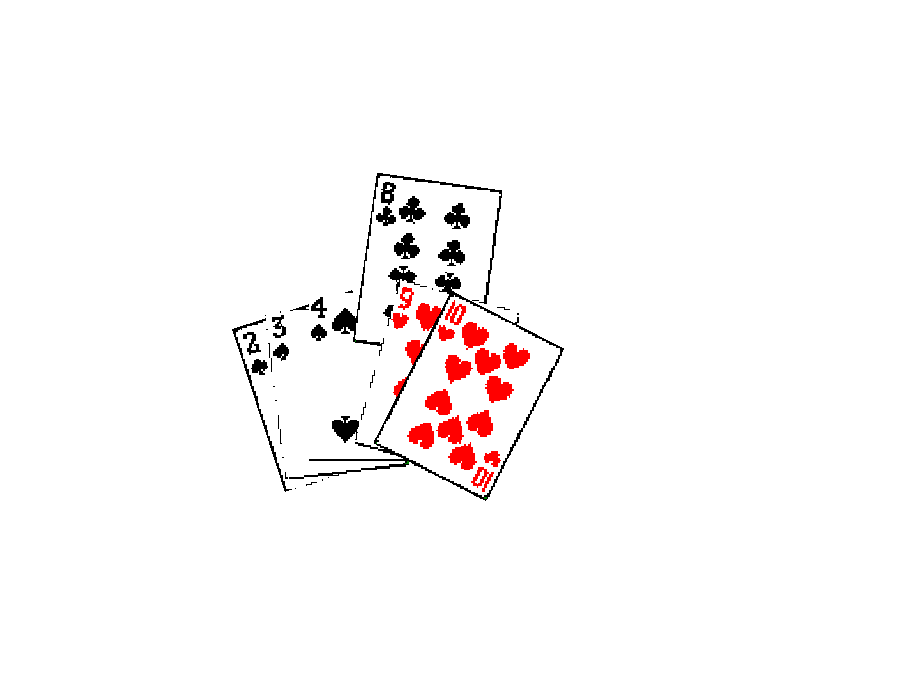
\includegraphics[scale=0.5]{img/hand-of-cards.eps}
  \caption{将草花8插入到一手牌中合适的位置。}
  \label{fig:hand-of-cards}
\end{figure}

根据这一思路,插入排序的算法可以这样给出:

\begin{algorithmic}
\Function{Sort}{$A$}
  \State $X \gets \phi$
  \For{each $x \in A$}
    \State \Call{Insert}{$X, x$}
  \EndFor
  \State \Return $X$
\EndFunction
\end{algorithmic}

我们在二叉搜索树一章曾经提到过folding的概念,插入排序也可以用这一概念来定义:

\be
  insert = foldL \quad insert \quad \phi
\ee

由于我们使用了$X$来存储排序结果,这一算法不是in-place排序算法。我们也可以把它改为in-place的。记待排序序列为$A = \{a_1, a_2, ... a_n\}$。

\begin{algorithmic}
\Function{Sort}{$A$}
  \For{$i \gets 2$ to $|A|$}
    \State insert $a_i$ to sorted sequence $\{a'_1, a'_2, ..., a'_{i-1} \}$
  \EndFor
\EndFunction
\end{algorithmic}

任何时候,当处理第$i$个元素的时候,所有$i$之前的元素都已经排好顺序了。我们不断将当前元素插入,直到处理完全部元素。这一过程如图\ref{fig:in-place-sort}所示。

\begin{figure}[htbp]
  \centering
  \includegraphics[scale=0.8]{img/in-place-sort.ps}
  \caption{左侧元素的顺序已经排好,不断将元素插入已序部份。}
  \label{fig:in-place-sort}
\end{figure}

这一过程中明显存在递归,因此可以表达为如下函数:

\be
sort(A) = \left \{
  \begin{array}
  {r@{\quad:\quad}l}
  \phi & A = \phi \\
  insert(sort(\{a_2, a_3, ...\}), a_1) & otherwise
  \end{array}
\right.
\ee

% ================================================================
% Insertion
% ================================================================
\section{插入}
\index{插入排序!插入}

我们尚未回答如何进行插入。人们还无法确切知道,大脑是如何在一手牌中快速找到插入位置的。

使用计算机,我们可以通过扫描找到插入位置。扫描时可以从左向右或者从右向左。但如果序列是用数组存储的,就必须从右向左进行扫描。

\begin{algorithmic}
\Function{Sort}{$A$}
  \For{$i \gets 2$ to $|A|$}
    \Comment{Insert $A[i]$ to sorted sequence $A[1...i-1]$}
    \State $x \gets A[i]$
    \State $j \gets i-1$
    \While{$j > 0 \land x < A[j]$ }
      \State $A[j+1] \gets A[j]$
      \State $j \gets j - 1$
    \EndWhile
    \State $A[j+1] \gets x$
  \EndFor
\EndFunction
\end{algorithmic}

有读者认为从左向右更加自然,但是这样性能上会出现问题。实际上,在数组中的任意位置插入元素是一个比较费时的操作。由于数组是连续存储元素的,如果需要在第$i$个位置插入元素$x$,我们需要把所有$i$后面的元素,包括第$i+1$、第$i+2$……都向右移动(shift)。之后,第$i$个位置才能空出来用以插入$x$。图\ref{fig:array-shift}描述了这一过程。

\begin{figure}[htbp]
  \centering
  \includegraphics[scale=0.7]{img/array-shift.ps}
  \caption{将元素$x$插入数组$A$中的第$i$个位置。}
  \label{fig:array-shift}
\end{figure}

从左向右扫描时,如果数组的长度为$n$,我们需要扫描前面$i$个元素,然后进行$n-i+1$次移动,最后将$x$插入到第$i$个位置。也就是说,从左向右扫描会遍历整个数组。相反,如果从右向左扫描,我们最多只需要检察$i$个元素,并且随着扫描将它们向右移动。

下面的Python例子程序实现了上述算法。

\lstset{language=Python}
\begin{lstlisting}
def isort(xs):
    n = len(xs)
    for i in range(1, n):
        x = xs[i]
        j = i - 1
        while j >= 0 and x < xs[j]:
            xs[j+1] = xs[j]
            j = j - 1
        xs[j+1] = x
\end{lstlisting}

这一实现也存在一些变形,例如下面的ANSI C语言的例子程序。但是它比我们给出的插入方法的操作次数多一些。

\lstset{language=C}
\begin{lstlisting}
void isort(Key* xs, int n){
  int i, j;
  for(i=1; i<n; ++i)
    for(j=i-1; j>=0 && xs[j+1] < xs[j]; --j)
      swap(xs, j, j+1);
}
\end{lstlisting}

这是因为交换函数\texttt{swap}通常使用一个中间变量来实现,如下:

\begin{lstlisting}
void swap(Key* xs, int i, int j){
  Key temp = xs[i];
  xs[i] = xs[j];
  xs[j] = temp;
}
\end{lstlisting}

若内循环的次数为$m$,上述ANSI C程序总共需要$3m$次赋值操作,而我们给出的算法及其Python实现使用shift来代替swap,它只需要$m+2$次赋值操作。

我们也可以提供单独的\textproc{Insert}()函数,然后在插入算法中调用它。我们略过这些实现细节,读者可以作为练习尝试这些不同的实现。

尽管有这些实现上的差异,从左向右也好,从右向左也好,所有这些插入算法的复杂度都是$O(n)$的,其中$n$为序列的长度。因此插入排序的总体复杂度为$O(n^2)$。

\begin{Exercise}

\begin{itemize}
\item 定义单独的插入函数,并在通用的插入排序算法中调用它。请尝试用命令式的方式和函数式的方式给出不同的实现。
\end{itemize}

\end{Exercise}

% ================================================================
% Improvement 1
% ================================================================

\section{改进一}
\index{插入排序!二分查找}

人的大脑是如何快速在一手牌中找到插入位置的?似乎不是逐一扫描。任何时刻,我们手中的牌都是已序的,因此我们可以用二分查找来搜索插入位置。

我们将来后面的章节中专门详细讨论搜索算法。本节仅仅对二分查找做一个简单介绍。

下面的排序算法改为调用二分查找来确定插入的位置:

\begin{algorithmic}
\Function{Sort}{$A$}
  \For{$i \gets 2$ to $|A|$}
    \State $x \gets A[i]$
    \State $p \gets $ \Call{Binary-Search}{$A[1...i-1], x$}
    \For{$j \gets i$ down to $p$}
      \State $A[j] \gets A[j-1]$
    \EndFor
    \State $A[p] \gets x$
  \EndFor
\EndFunction
\end{algorithmic}

我们不再逐一扫描元素,考虑数组中的片断$\{A[1], ..., A[i-1] \}$已经有序了。假设它们是单调增的,我们需要找到一个位置$j$使得$A[j-1] \leq x \leq A[j]$。我们可以先检查中间的元素$A[\lfloor i/2 \rfloor]$。如果$x$比它小,我们需要接下来递归地在前一半序列进行二分查找;否则我们需要查找后一半序列。

由于我们每次都砍掉一半元素,所以这一过程需要$O(\lg n)$的时间来找到插入的位置。

\begin{algorithmic}
\Function{Binary-Search}{$A, x$}
  \State $l \gets 1$
  \State $u \gets 1+|A|$
  \While{$l < u$}
    \State $m \gets \lfloor \frac{l+u}{2} \rfloor$
    \If{$A[m] = x$}
      \State \Return $m$ \Comment{Find a duplicated element}
    \ElsIf{$A[m] < x$}
      \State $l \gets m+1$
    \Else
      \State $u \gets m$
    \EndIf
  \EndWhile
  \State \Return $l$
\EndFunction
\end{algorithmic}

The improved insertion sort algorithm is still bound to $O(n^2)$,
compare to previous section, which we use $O(n^2)$ times comparison and
$O(n^2)$ moves, with binary search, we just use $O(n \lg n)$ times
comparison and $O(n^2)$ moves.

The Python program regarding to this algorithm is given below.

\lstset{language=Python}
\begin{lstlisting}
def isort(xs):
    n = len(xs)
    for i in range(1, n):
        x = xs[i]
        p = binary_search(xs[:i], x)
        for j in range(i, p, -1):
            xs[j] = xs[j-1]
        xs[p] = x

def binary_search(xs, x):
    l = 0
    u = len(xs)
    while l < u:
        m = (l+u)/2
        if xs[m] == x:
            return m
        elif xs[m] < x:
            l = m + 1
        else:
            u = m
    return l
\end{lstlisting}

\begin{Exercise}
Write the binary search in recursive manner. You needn't use purely functional
programming language.
\end{Exercise}

% ================================================================
% Improvement 2
% ================================================================

\section{Improvement 2}
\index{Insertion sort!linked-list setting}

Although we improve the search time to $O(n \lg n)$ in previous section, the
number of moves is still $O(n^2)$. The reason of why movement takes so long
time, is because the sequence is stored in plain array. The nature of array
is continuously layout data structure, so the insertion operation is expensive.
This hints us that we can use linked-list setting to represent the sequence.
It can improve the insertion operation from $O(n)$ to constant time $O(1)$.

\be
  insert(A, x) = \left \{
  \begin{array}
  {r@{\quad:\quad}l}
  \{ x \} & A = \phi \\
  \{ x \} \cup A & x < A_1 \\
  \{ A_1 \} \cup insert(\{ A_2, A_3, ... A_n\}, x)& otherwise
  \end{array}
\right.
\ee

Translating the algorithm to Haskell yields the below program.

\lstset{language=Haskell}
\begin{lstlisting}
insert :: (Ord a) => [a] -> a -> [a]
insert [] x = [x]
insert (y:ys) x = if x < y then x:y:ys else y:insert ys x
\end{lstlisting}

And we can complete the two versions of insertion sort program based on
the first two equations in this chapter.

\begin{lstlisting}
isort [] = []
isort (x:xs) = insert (isort xs) x
\end{lstlisting}

Or we can represent the recursion with folding.

\begin{lstlisting}
isort = foldl insert []
\end{lstlisting}

Linked-list setting solution can also be described imperatively. Suppose
function \textproc{Key}($x$), returns the value of element stored in node
$x$, and \textproc{Next}($x$) accesses the next node in the linked-list.

\begin{algorithmic}
\Function{Insert}{$L, x$}
  \State $p \gets NIL$
  \State $H \gets L$
  \While{$L \neq NIL \land $ \Call{Key}{$L$} $<$ \Call{Key}{$x$}}
    \State $p \gets L$
    \State $L \gets $ \Call{Next}{$L$}
  \EndWhile
  \State \Call{Next}{$x$} $\gets L$
  \If{$p \neq NIL$}
    \State $H \gets x$
  \Else
    \State \Call{Next}{$p$} $\gets x$
  \EndIf
  \State \Return $H$
\EndFunction
\end{algorithmic}

For example in ANSI C, the linked-list can be defined as the following.

\lstset{language=C}
\begin{lstlisting}
struct node{
  Key key;
  struct node* next;
};
\end{lstlisting}

Thus the insert function can be given as below.

\begin{lstlisting}
struct node* insert(struct node* lst, struct node* x){
  struct node *p, *head;
  p = NULL;
  for(head = lst; lst && x->key > lst->key; lst = lst->next)
    p = lst;
  x->next = lst;
  if(!p)
    return x;
  p->next = x;
  return head;
}
\end{lstlisting}

Instead of using explicit linked-list such as by pointer or reference
based structure. Linked-list can also be realized by another index array.
For any array element $A_i$, $Next_i$ stores the index of next element
follows $A_i$. It means $A_{Next_i}$ is the next element after $A_i$.

The insertion algorithm based on this solution is given like below.

\begin{algorithmic}
\Function{Insert}{$A, Next, i$}
  \State $j \gets \perp$
  \While{$Next_j \neq NIL \land A_{Next_j} < A_i$}
    \State $j \gets Next_j$
  \EndWhile
  \State $Next_i \gets Next_j$
  \State $Next_j \gets i$
\EndFunction
\end{algorithmic}

Here $\perp$ means the head of the $Next$ table.
And the relative Python program for this algorithm is given as the following.

\lstset{language=Python}
\begin{lstlisting}
def isort(xs):
    n = len(xs)
    next = [-1]*(n+1)
    for i in range(n):
        insert(xs, next, i)
    return next

def insert(xs, next, i):
    j = -1
    while next[j] != -1 and xs[next[j]] < xs[i]:
        j = next[j]
    next[j], next[i] = i, next[j]
\end{lstlisting}

Although we change the insertion operation to constant time by using
linked-list. However, we have to traverse the linked-list to find the
position, which results $O(n^2)$ times comparison. This is because
linked-list, unlike array, doesn't support random access. It means we
can't use binary search with linked-list setting.

\begin{Exercise}
\begin{itemize}
\item Complete the insertion sort by using linked-list insertion function
in your favorate imperative programming language.
\item The index based linked-list return the sequence of rearranged index
as result. Write a program to re-order the original array of elements from
this result.
\end{itemize}
\end{Exercise}

% ================================================================
% Final improvement
% ================================================================

\section{Final improvement by binary search tree}
\index{Insertion sort!binary search tree}

It seems that we drive into a corner. We must improve both the comparison
and the insertion at the same time, or we will end up with $O(n^2)$ performance.

We must use binary search, this is the only way to improve the comparison
time to $O(\lg n)$. On the other hand, we must change the data structure,
because we can't achieve constant time insertion at a position with
plain array.

This remind us about our 'hello world' data structure, binary search tree.
It naturally support binary search from its definition. At the same time,
We can insert a new leaf in binary search tree in $O(1)$ constant time
if we already find the location.

So the algorithm changes to this.

\begin{algorithmic}
\Function{Sort}{$A$}
  \State $T \gets \phi$
  \For{each $x \in A$}
    \State $T \gets $ \Call{Insert-Tree}{$T, x$}
  \EndFor
  \State \Return \Call{To-List}{$T$}
\EndFunction
\end{algorithmic}

Where \textproc{Insert-Tree}() and \textproc{To-List}() are described in
previous chapter about binary search tree.

As we have analyzed for binary search tree, the performance of tree sort
is bound to $O(n \lg n)$, which is the lower limit of comparison based
sort\cite{Knuth}.

\section{Short summary}
In this chapter, we present the evolution process of insertion sort. Insertion
sort is well explained in most textbooks as the first sorting algorithm.
It has simple and straightforward idea, but the performance is quadratic.
Some textbooks stop here, but we want to show that there exist ways to improve
it by different point of view. We first try to save the comparison time
by using binary search, and then try to save the insertion operation by
changing the data structure to linked-list. Finally, we combine these
two ideas and evolute insertion sort to tree sort.

\begin{thebibliography}{99}

\bibitem{wiki-bubble-sort}
http://en.wikipedia.org/wiki/Bubble\_sort

\bibitem{CLRS}
Thomas H. Cormen, Charles E. Leiserson, Ronald L. Rivest and Clifford Stein.
``Introduction to Algorithms, Second Edition''. ISBN:0262032937. The MIT Press. 2001

\bibitem{Knuth}
Donald E. Knuth. ``The Art of Computer Programming, Volume 3: Sorting and Searching (2nd Edition)''. Addison-Wesley Professional; 2 edition (May 4, 1998) ISBN-10: 0201896850 ISBN-13: 978-0201896855

\end{thebibliography}

\ifx\wholebook\relax\else
\end{document}
\fi


\ifx\wholebook\relax \else
% ------------------------

\documentclass[UTF8]{article}
%------------------- Other types of document example ------------------------
%
%\documentclass[twocolumn]{IEEEtran-new}
%\documentclass[12pt,twoside,draft]{IEEEtran}
%\documentstyle[9pt,twocolumn,technote,twoside]{IEEEtran}
%
%-----------------------------------------------------------------------------
%
% loading packages
%

\RequirePackage{ifpdf}
\RequirePackage{ifxetex}

%
%
\ifpdf
  \RequirePackage[pdftex,%
       bookmarksnumbered,%
              colorlinks,%
          linkcolor=blue,%
              hyperindex,%
        plainpages=false,%
       pdfstartview=FitH]{hyperref}
\else\ifxetex
  \RequirePackage[bookmarksnumbered,%
               colorlinks,%
           linkcolor=blue,%
               hyperindex,%
         plainpages=false,%
        pdfstartview=FitH]{hyperref}
\else
  \RequirePackage[dvipdfm,%
        bookmarksnumbered,%
               colorlinks,%
           linkcolor=blue,%
               hyperindex,%
         plainpages=false,%
        pdfstartview=FitH]{hyperref}
\fi\fi
%\usepackage{hyperref}

% other packages
%--------------------------------------------------------------------------
\usepackage{graphicx, color}
\usepackage{subfig}
\usepackage{tikz}
\usetikzlibrary{matrix,positioning}

\usepackage{amsmath, amsthm, amssymb} % for math
\usepackage{exercise} % for exercise
\usepackage{import} % for nested input

%
% for programming
%
\usepackage{verbatim}
\usepackage{listings}
%\usepackage{algorithmic} %old version; we can use algorithmicx instead
\usepackage{algorithm}
\usepackage[noend]{algpseudocode} %for pseudo code, include algorithmicsx automatically
\usepackage{appendix}
\usepackage{makeidx} % for index support
\usepackage{titlesec}

\usepackage[cm-default]{fontspec}
\usepackage{xunicode}

% detect and select Chinese font
% ------------------------------
% the following cmd can list all availabe Chinese fonts in host.
% fc-list :lang=zh
\def\myfont{STHeiti}  % Under Mac OS X
\def\linuxfallback{WenQuanYi Micro Hei} % Under Linux
\def\winfallback{SimSun} % Under Windows
\suppressfontnotfounderror1 % Avoid setting exit code (error level) to break make process
\count255=\interactionmode
\batchmode
\font\foo="\myfont"\space at 10pt
\ifx\foo\nullfont
  \font\foo = "\linuxfallback"\space at 10pt
  \ifx\foo\nullfont
    \font\foo = "\winfallback"\space at 10pt
    \ifx\foo\nullfont
      \errorstopmode
      \errmessage{no suitable Chinese font found}
    \else
      \let\myfont=\winfallback % Windows
    \fi
  \else
    \let\myfont=\linuxfallback % Linux
  \fi
\fi
\interactionmode=\count255
\setmainfont[Mapping=tex-text]{\myfont}

\XeTeXlinebreaklocale "zh"  % to solve the line breaking issue
\XeTeXlinebreakskip = 0pt plus 1pt minus 0.1pt

\titleformat{\paragraph}
{\normalfont\normalsize\bfseries}{\theparagraph}{1em}{}
\titlespacing*{\paragraph}
{0pt}{3.25ex plus 1ex minus .2ex}{1.5ex plus .2ex}

\lstdefinelanguage{Smalltalk}{
  morekeywords={self,super,true,false,nil,thisContext}, % This is overkill
  morestring=[d]',
  morecomment=[s]{"}{"},
  alsoletter={\#:},
  escapechar={!},
  literate=
    {BANG}{!}1
    {UNDERSCORE}{\_}1
    {\\st}{Smalltalk}9 % convenience -- in case \st occurs in code
    % {'}{{\textquotesingle}}1 % replaced by upquote=true in \lstset
    {_}{{$\leftarrow$}}1
    {>>>}{{\sep}}1
    {^}{{$\uparrow$}}1
    {~}{{$\sim$}}1
    {-}{{\sf -\hspace{-0.13em}-}}1  % the goal is to make - the same width as +
    %{+}{\raisebox{0.08ex}{+}}1		% and to raise + off the baseline to match -
    {-->}{{\quad$\longrightarrow$\quad}}3
	, % Don't forget the comma at the end!
  tabsize=2
}[keywords,comments,strings]

% for better Haskell code outlook
\lstdefinelanguage{Haskell}{
  basicstyle=\small\ttfamily,
  flexiblecolumns=false,
  basewidth={0.5em,0.45em},
  literate={+}{{$+$}}1 {/}{{$/$}}1 {*}{{$*$}}1 {=}{{$=$}}1
           {>}{{$>$}}1 {<}{{$<$}}1 {\\}{{$\lambda$}}1
           {\\\\}{{\char`\\\char`\\}}1
           {->}{{$\rightarrow$}}2 {>=}{{$\geq$}}2 {<-}{{$\leftarrow$}}2
           {<=}{{$\leq$}}2 {=>}{{$\Rightarrow$}}2
           {\ .}{{$\circ$}}2 {\ .\ }{{$\circ$}}2
           {>>}{{>>}}2 {>>=}{{>>=}}2
           {|}{{$\mid$}}1
}[keywords,comments,strings]

\lstloadlanguages{C, C++, Lisp, Haskell, Python, Smalltalk}

\lstset{
  showstringspaces = false
}

% ======================================================================

\def\BibTeX{{\rm B\kern-.05em{\sc i\kern-.025em b}\kern-.08em
    T\kern-.1667em\lower.7ex\hbox{E}\kern-.125emX}}

%
% mathematics
%
\newcommand{\be}{\begin{equation}}
\newcommand{\ee}{\end{equation}}
\newcommand{\bmat}[1]{\left( \begin{array}{#1} }
\newcommand{\emat}{\end{array} \right) }
\newcommand{\VEC}[1]{\mbox{\boldmath $#1$}}

% numbered equation array
\newcommand{\bea}{\begin{eqnarray}}
\newcommand{\eea}{\end{eqnarray}}

% equation array not numbered
\newcommand{\bean}{\begin{eqnarray*}}
\newcommand{\eean}{\end{eqnarray*}}

\newtheorem{theorem}{Theorem}[section]
\newtheorem{lemma}[theorem]{Lemma}
\newtheorem{proposition}[theorem]{Proposition}
\newtheorem{corollary}[theorem]{Corollary}


\setcounter{page}{1}

\begin{document}

%--------------------------

% ================================================================
%                 COVER PAGE
% ================================================================

\title{并不复杂的红黑树}

\author{刘新宇
\thanks{{\bfseries 刘新宇} \newline
  Email: liuxinyu95@gmail.com \newline}
  }

\maketitle
\fi

\markboth{红黑树}{初等算法}

\ifx\wholebook\relax
\chapter{并不复杂的红黑树}
\numberwithin{Exercise}{chapter}
\fi

% ================================================================
%                 Introduction
% ================================================================
\section{简介}
\label{introduction} \index{红黑树}

\subsection{二叉搜索树的不足}
上一章中,我们给出了一个例子:统计一篇文章中每个单词出现的次数。思路是把二叉搜索树当作一个字典来计数。

一个自然的想法是使用二叉搜索树来处理电话黄页\footnote{一种公共发布的电话号码簿,因用黄色纸张印刷所以称为黄页。},并用它来查询某联系人的电话。

可以把上一章中的例子代码稍做改动来实现这一功能:

\begin{lstlisting}
int main(int, char** ) {
  ifstream f("yp.txt");
  map<string, string> dict;
  string name, phone;
  while(f>>name && f>>phone)
    dict[name]=phone;
  for(;;) {
    cout<<"\nname: ";
    cin>>name;
    if(dict.find(name) == dict.end())
      cout<<"not found";
    else
      cout<<"phone: "<<dict[name];
  }
}
\end{lstlisting}

这段程序运行良好。但是,如果我们把STL库提供的map换成普通的二叉搜索树,程序的性能就变差了,尤其是搜索诸如Zara、Zed、Zulu等姓名时特别明显。

这是因为电话黄页通常是按照字典字母顺序(lexicographic order)印刷的。因此姓名实际上是按照升序排列的。如果我们依次把数字1, 2, 3, ..., $n$插入二叉搜索树,就会得到一棵如图\ref{fig:unbalanced-tree}所示的树。

\begin{figure}[htbp]
    \centering
	\includegraphics[scale=0.5]{img/unbalanced.ps}
    \caption{不平衡的树} \label{fig:unbalanced-tree}
\end{figure}

这是一棵极不平衡的二叉树。对于高度为$h$的二叉搜索树,查找算法的复杂度为$O(h)$。如果树比较平衡,我们就能够达到$O(\lg n)$的性能。但在这一极端情况下,查找的性能退化为$O(n)$。几乎和普通的链表一样。

\begin{Exercise}

\begin{itemize}
\item 对于巨大的电话黄页列表,为了加快速度,一个想法是使用两个并发的任务(task,可以是线程或进程)。一个任务从头部向后读姓名――电话信息,另外一个任务从尾部向前读。当两个任务在中间相遇时程序结束。这样构建出的二叉搜索树是什么样子的?如果我们把黄页列表分割成更多片断,使用更多的任务会得到什么结果?
\item 参考图\ref{fig:unbalanced-trees}中的一些不平衡树,你能找到更多的情况造成二叉搜索树表现不佳么?
\end{itemize}

\end{Exercise}

\begin{figure}[htbp]
       \centering
       \subfloat[]{\includegraphics[scale=0.4]{img/unbalanced-2.ps}}
       \subfloat[]{\includegraphics[scale=0.4]{img/unbalanced-zigzag.ps}} \\
       \subfloat[]{\includegraphics[scale=0.4]{img/unbalanced-3.ps}}
       \caption{一些不平衡的二叉树}
       \label{fig:unbalanced-trees}
\end{figure}

\subsection{如何保证树的平衡}

为了避免出现上面描述的不平衡情况,我们可以预先使用随机算法将输入序列打乱(参见\cite{CLRS}的12.4节)。但是有时无法使用这个方法,例如序列是由用户交互输入的,每当用户输入一个key后,树就会被更新。也就是说,树是随着用户输入逐步构建的。

人们已经发现了好几种方法用于解决二叉搜索树的平衡问题。由很多方法依赖于二叉树的旋转(rotation)操作。旋转操作可以在保持元素顺序的情况下,改变树的结构。因此可以用来提高二叉搜索树的平衡性。

本章介绍红黑树――一种被广泛使用的自平衡二叉搜索树(self-adjusting balanced binary search tree)。下一章我们介绍另外一种自平衡树――AVL树。在后面介绍二叉堆的章节中,我们还会遇到另外一种有趣的树――splay树,它能够随着操作,逐渐使得树变得越来越平衡。

\subsection{树的旋转}
\index{树的旋转}

\begin{figure}[htbp]
   \centering
   \setlength{\unitlength}{1cm}
   \begin{picture}(10, 4)
   \put(5, 2){$\Longleftrightarrow$}
   \subfloat[]{\includegraphics[scale=0.4]{img/rotate-r.ps}}
   \subfloat[]{\includegraphics[scale=0.4]{img/rotate-l.ps}}
   \end{picture}
   \\
   \begin{picture}(1, 0.5)\end{picture} %pad
   \caption{树的旋转,左旋操作将左侧图中的树变换为右侧的树;右旋操作是左旋的逆变换。}
   \label{fig:tree-rotation}
\end{figure}

树的旋转是一种特殊的操作,它在保持中序遍历结果不变的情况下,改变树的结构。这是因为存在多个不同的二叉搜索树对应到一个特定的中序遍历顺序。图\ref{fig:tree-rotation}描述了旋转操作。图中左侧的二叉搜索树,经过左旋可以变换为右侧的树,而右旋是左旋的逆变换。

旋转操作可以用过程式的方法来描述。通过使用模式匹配(pattern matching)我们也可以用简单的函数来定义它们。将非空的二叉树记为三元组$T=(T_l, k, T_r)$,下面的函数定义了左右旋转。

\be
rotateL(T) = \left \{
  \begin{array}
  {r@{\quad:\quad}l}
  ((a, X, b), Y, c) & T = (a, X, (b, Y, c)) \\
  T & otherwise
  \end{array}
\right .
\ee

\be
rotateR(T) = \left \{
  \begin{array}
  {r@{\quad:\quad}l}
  (a, X, (b, Y, c)) & T = ((a, X, b), Y, c)) \\
  T & otherwise
  \end{array}
\right .
\ee

用伪代码描述时,除了左右分支和key,还需要设置好父节点。

\begin{algorithmic}[1]
\Function{Left-Rotate}{$T, x$}
  \State $p \gets$ \Call{Parent}{$x$}
  \State $y \gets$ \Call{Right}{$x$} \Comment{Assume $y \ne NIL$}
  \State $a \gets$ \Call{Left}{$x$}
  \State $b \gets$ \Call{Left}{$y$}
  \State $c \gets$ \Call{Right}{$y$}
  \State \Call{Replace}{$x, y$}
  \State \Call{Set-Children}{$x, a, b$}
  \State \Call{Set-Children}{$y, x, c$}
  \If{$p = NIL$}
    \State $T \gets y$
  \EndIf
  \State \Return $T$
\EndFunction

\Statex

\Function{Right-Rotate}{$T, y$}
  \State $p \gets$ \Call{Parent}{$y$}
  \State $x \gets$ \Call{Left}{$y$} \Comment{Assume $x \ne NIL$}
  \State $a \gets$ \Call{Left}{$x$}
  \State $b \gets$ \Call{Right}{$x$}
  \State $c \gets$ \Call{Right}{$y$}
  \State \Call{Replace}{$y, x$}
  \State \Call{Set-Children}{$y, b, c$}
  \State \Call{Set-Children}{$x, a, y$}
  \If{$p = NIL$}
    \State $T \gets x$
  \EndIf
  \State \Return $T$
\EndFunction

\Statex

\Function{Set-Left}{$x, y$}
  \State \Call{Left}{$x$} $\gets y$
  \If{$y \ne NIL$}
    \Call{Parent}{$y$} $\gets x$
  \EndIf
\EndFunction

\Statex

\Function{Set-Right}{$x, y$}
  \State \Call{Right}{$x$} $\gets y$
  \If{$y \ne NIL$}
    \Call{Parent}{$y$} $\gets x$
  \EndIf
\EndFunction

\Statex

\Function{Set-Children}{$x, L, R$}
  \State \Call{Set-Left}{$x, L$}
  \State \Call{Set-Right}{$x, R$}
\EndFunction

\Statex

\Function{Replace}{$x, y$}
  \If{\Call{Parent}{$x$} $= NIL$}
    \If{$y \ne NIL$}
      \Call{Parent}{$y$} $\gets NIL$
    \EndIf
  \ElsIf{\textproc{Left}(\Call{Parent}{$x$}) $= x$}
    \State \textproc{Set-Left}(\Call{Parent}{$x$}, $y$)
  \Else
    \State \textproc{Set-Right}(\Call{Parent}{$x$}, $y$)
  \EndIf
  \State \Call{Parent}{$x$} $\gets NIL$
\EndFunction
\end{algorithmic}

对比伪代码和使用模式匹配的函数,后者主要从树结构变化的角度出发,而前者集中于描述变换的过程。如本章题目所讲,红黑树并不像看起来那样复杂。很多教科书使用传统的过程式方法来讲解红黑树,需要处理许多不同的情况。每种情况都必须仔细处理节点种的数据。如果换成函数式的思路,虽然会牺牲一些性能,但很多问题会变得简单直观。

本章中的大部份内容来自Chris Okasaki的成果\cite{okasaki}。

% ================================================================
% Definition
% ================================================================
\section{红黑树的定义}
\index{红黑树}

红黑树式一种自平衡二叉搜索树\cite{wiki}\footnote{红黑树是2-3-4树的等价形式(有关2-3-4树,可参考B树一章)。也就是说,对于任一2-3-4树,都存在至少一个红黑树与之有着相同顺序的元素。}。通过对节点进行着色和旋转,红黑树可以简单直观地保持树的平衡。

我们可以在普通的二叉搜索树上增加一个颜色信息。一个节点可以被涂成红色或黑色。如果一棵二叉搜索树满足下面的全部5条性质,我们称之为红黑树\cite{CLRS}。
\index{红黑树!红黑性质}

\begin{enumerate}
\item 任一节点要么是红色,要么是黑色。
\item 根节点为黑色。
\item 所有的叶节点(NIL节点)为黑色。
\item 如果一个节点为红色,则它的两个子节点都是黑色。
\item 对任一节点,从它出发到所有叶子节点的路径上包含相同数量的黑色节点。
\end{enumerate}

为什么这5条性质能保证红黑树的平衡性呢?因为它们有一个关键的特性:从根节点出发到达叶节点的所有路径中,最长路径不会超过最短路径长度的两倍。

注意到第四条性质,它意味着不存在两个连续的红色节点。因此,最短的路径只含有黑色的节点,任何比最短路径长的路径上都分散有一些红色节点。根据性质五,从根节点出发的所有的路径都含有相同数量的黑色节点,这就最终保证了没有任何路径超过最短路径长度的两倍\cite{wiki}。图\ref{fig:rbt-example}的例子展示了一棵红黑树。

\begin{figure}[htbp]
  \centering
  \includegraphics[scale=0.5]{img/rbt-example.ps}
  \caption{红黑树} \label{fig:rbt-example}
\end{figure}

红黑树沿用所有二叉搜索树中不改变树结构的操作,包括查找、获取最大、最小值等。只有插入和删除操作是特殊的。

如前面的单词统计的例子所示,有很多集合(set)和map容器是使用红黑树来实现的。包括C++标准库中STL\cite{sgi-stl}。

由于只增加了一个颜色信息,我们可以复用二叉搜索树的节点定义。如下面的C++代码所示:

\lstset{language=C++}
\begin{lstlisting}
enum Color {Red, Black};

template <class T>
struct node{
  Color color;
  T key;
  node* left;
  node* right;
  node* parent;
};
\end{lstlisting}

对于函数式环境,我们可以在代数数据类型(algebraic data type)的定义中增加颜色参数,如下面的Haskell例子所示:

\lstset{language=Haskell}
\begin{lstlisting}
data Color = R | B
data RBTree a = Empty
              | Node Color (RBTree a) a (RBTree a)
\end{lstlisting}

\begin{Exercise}

\begin{itemize}
\item 利用红黑树的性质证明$n$个节点的红黑树的高度不会超过$2 \lg (n+1)$。
\end{itemize}

\end{Exercise}

% ================================================================
%                 Insertion
% ================================================================
\section{插入}
\index{红黑树!插入}

由于插入操作会改变二叉搜索树的结构,树有可能因此变得不平衡。为了保持红黑树的性质,我们需要在插入操作后进行变换来修复平衡问题。

当插入一个key时,可以总是把新节点染成红色。只要它不是根节点,除了第四条外的所有红黑树性质都可以满足。唯一的问题就是可能引入两个相邻的红色节点。

函数式和命令式实现使用不同的方法来修复平衡。前者直观简单,但是存在一点性能损失;后者有些复杂,但是具有更高的性能。大多数的算法书籍介绍后一种方法。本章中,我们关注函数式的方法,并展示这一方法极为简洁的特性。我们也会给出传统的命令式实现以作为对比。

Chris Okasaki指出,共有四种情况会违反红黑树的第四条性质。它们都带有两个相邻的红色节点。而且,它们可以被统一修复为一个形式\cite{okasaki},如图 \ref{fig:insert-fix}所示。

\begin{figure}[htbp]
  \centering
     \setlength{\unitlength}{1cm}
     \begin{picture}(15, 15)
        % arrows
        \put(4.5, 9.5){\vector(1, -1){1}}
        \put(4.5, 5){\vector(1, 1){1}}
        \put(10, 9.5){\vector(-1, -1){1}}
        \put(10, 5){\vector(-1, 1){1}}
        % graphics
	\put(0, 7){\includegraphics[scale=0.5]{img/insert-ll.ps}}
        \put(0, 0){\includegraphics[scale=0.5]{img/insert-lr.ps}}
        \put(7, 7){\includegraphics[scale=0.5]{img/insert-rr.ps}}
        \put(8.5, 0){\includegraphics[scale=0.5]{img/insert-rl.ps}}
        \put(2, 5){\includegraphics[scale=0.5]{img/insert-fixed.ps}}
      \end{picture}
     \caption{插入后需要修复的四种情况} \label{fig:insert-fix}
\end{figure}

注意到这一变换会把红色向上“移动”一层。因此它是一种自底向上的递归修复,最后一步会把根节点染成红色。根据红黑树的第二条性质,根节点必须是黑色的。因此我们最后要把根节点再染回黑色。为了方便,我们把节点的颜色记为$\mathcal{C}$,它有两个值,黑色$\mathcal{B}$和红色$\mathcal{R}$。这样一棵非空的红黑树可以表达为一个四元组$T=(\mathcal{C}, T_l, k, T_r)$。

\be
balance(T) = \left \{
  \begin{array}
  {r@{\quad:\quad}l}
  (\mathcal{R}, (\mathcal{B}, A, x, B), y, (\mathcal{B}, C, z, D)) & match(T) \\
  T & otherwise
  \end{array}
\right .
\ee

其中,函数$match(T)$用以判断树是否符合图\ref{fig:insert-fix}中的四种需要修复的情况。定义如下:

\[
match(T) = \left \{ T = \begin{array}{l}
         (\mathcal{B}, (\mathcal{R}, (\mathcal{R}, A, x, B), y, C), z, D) \lor \\
         (\mathcal{B}, (\mathcal{R}, A, x, (\mathcal{R}, B, y, C), z, D)) \lor \\
         (\mathcal{B}, A, x, (\mathcal{R}, B, y, (\mathcal{R}, C, z, D))) \lor \\
         (\mathcal{B}, A, x, (\mathcal{R}, (\mathcal{R}, B, y, C), z, D)) \\
         \end{array} \right \}
\]

定义好函数$balance(T)$后,我们就可以修改普通二叉搜索树的插入函数,使其支持红黑树的插入。

\be
insert(T, k) = makeBlack(ins(T, k))
\ee

其中$ins(T, k)$函数定义如下:

\be
ins(T, k) = \left \{
  \begin{array}
  {r@{\quad:\quad}l}
  (\mathcal{R}, \phi, k, \phi) & T = \phi \\
  balance((ins(T_l, k), k', T_r)) & k < k' \\
  balance((T_l, k', ins(T_r, k))) & otherwise
  \end{array}
\right.
\ee

如果待插入的树为空,则创建一个新的红色节点,节点的key就是待插入的$k$;否则,记树的左右分支和key分别为$T_l$、$T_r$和$k'$,我们比较$k$和$k'$的大小,递归地将它插入的分支中,然后再用$balance$函数恢复平衡。最后,我们使用$makeBlack(T)$函数把根节点染成黑色。

\be
makeBlack(T) = (\mathcal{B}, T_l, k, T_r)
\ee

在支持模式匹配的语言中,例如Haskell,插入算法可以实现为下面的程序:

\lstset{language=Haskell}
\begin{lstlisting}
insert t x = makeBlack $ ins t where
    ins Empty = Node R Empty x Empty
    ins (Node color l k r)
        | x < k     = balance color (ins l) k r
        | otherwise = balance color l k (ins r) --[3]
    makeBlack(Node _ l k r) = Node B l k r

balance B (Node R (Node R a x b) y c) z d =
                Node R (Node B a x b) y (Node B c z d)
balance B (Node R a x (Node R b y c)) z d =
                Node R (Node B a x b) y (Node B c z d)
balance B a x (Node R b y (Node R c z d)) =
                Node R (Node B a x b) y (Node B c z d)
balance B a x (Node R (Node R b y c) z d) =
                Node R (Node B a x b) y (Node B c z d)
balance color l k r = Node color l k r
\end{lstlisting} %$

程序中的\texttt{balance}函数略微有些该动,它的参数不是一棵树,而是节点的颜色、左侧分支、key和右侧分支。这样可以节省一对boxing和unboxing的操作。

例子程序没有处理试图插入重复key的情况。实际中,我们可以选择覆盖,也可以跳过不做处理,还可以选择在节点中用一个链表来来存储重复的数据\cite{CLRS}。

图\ref{fig:insert-example}中给出了两个红黑树的例子。左侧的是按照顺序将11, 2, 14, 1, 7, 5, 8, 4这些值插入的结果。右侧的是将序列1, 2, ..., 8插入的结果。可以看到,即使输入已序序列,产生的红黑树仍然保持了平衡。

\begin{figure}[htbp]
  \centering
  \includegraphics[scale=0.5]{img/insert-haskell.ps}
  \caption{根据不同的序列,使用插入算法产生的两棵红黑树} \label{fig:insert-example}
\end{figure}

通过将四种不同的不平衡树统一变换成同一种形式,我们得到了一个极为简洁的算法。即使在不支持模式匹配的语言中,我们仍然可以用编程检验树是否满足一定的模式。这样得到的结果和传统方法相比,仍然要简洁很多。读者可以参考本章附带的Lisp方言Scheme的例子代码。

对于含有$n$个节点的红黑树,这一插入算法的复杂度为$O(\lg n)$。

\begin{Exercise}

\begin{itemize}
\item 使用一种命令式语言,例如C、C++或Python来实现本节介绍的插入算法。注意:如果语言本身不支持模式匹配,需要编程检查四种不同的情况。
\end{itemize}

\end{Exercise}

% ================================================================
%                 Deletion
% ================================================================

\section{删除}
\index{红黑树!删除}

在上一章我们曾指出,二叉搜索树的删除操作只在imperative的环境下才有意义。这一结论同样适用于红黑树。大多数情况下,通常一次性将树构建好,然后频繁地进行查找。Okasaki曾经解释过为什么他没有给出红黑树的删除算法\cite{okasaki-blog}。其中一个原因就是删除比插入要麻烦得多。

我们希望通过本节的介绍,使读者了解到,在纯函数式的环境中,删除算法是可以实现的。纯函数式数据结构决定了树不会真的被改变,我们实际上是重建了一棵树\footnote{大多数函数式编程环境通过使用persistent,可以复用树中没有改变的部份,从而减小重建的开销。}。实际应用中,往往是由用户(也就是编程者)来决定使用那种具体的方案。例如,我们可以不做任何操作,而仅仅给每个要删除的节点做一个标记。当带有删除标记的节点超过50\%的时候,用所有未标记的节点重建一棵树。

不仅是函数式环境,imperative的删除算法也比插入算法要复杂。这主要是因为在删除时,我们面临更多的情况需要修复平衡。删除也会破坏红黑树的性质,因此需要后继的处理以恢复平衡。

本节介绍的删除算法主要来自\cite{lyn}。只有在删除一个黑色的节点时才会引发问题。因为这样会破坏红黑树的第五条性质,使得某一路径上的黑色节点数目少于其他的路径。

在删除一个黑色节点时,我们可以通过引入“双重黑色”\cite{CLRS}的概念来恢复第五条红黑树性质。也就是说,虽然节点被删除了,我们把它的黑色保存在它的父节点中。如果父节点是红色的,我们将其变为黑色;但如果父节点已经是黑色的,它就会变成一个“双重黑色”的节点。

为了表达双重黑色的节点,我们需要修改一下红黑树的定义,如下面的Haskell示例代码:

\lstset{language=Haskell}
\begin{lstlisting}
data Color = R | B | BB -- BB: doubly black for deletion
data RBTree a = Empty | BBEmpty -- doubly black empty
              | Node Color (RBTree a) a (RBTree a)
\end{lstlisting}

删除一个节点时,我们先调用普通二叉搜索树的删除算法。如果被删除节点时黑色的,我们接下来进行修复以保持红黑树的第五条性质。删除函数定义如下:

\be
delete(T, k) = blackenRoot(del(T, k))
\ee

其中

\be
del(T, k) = \left \{
  \begin{array}
  {r@{\quad:\quad}l}
  \phi & T = \phi \\
  fixBlack^2((\mathcal{C}, del(T_l, k), k', T_r)) & k < k' \\
  fixBlack^2((\mathcal{C}, T_l, k', del(T_r, k))) & k > k' \\
  \left \{
    \begin{array}{r@{\quad:\quad}l}
    mkBlk(T_r) & \mathcal{C} = \mathcal{B} \\
    T_r & otherwise
    \end{array}
  \right. & T_l = \phi \\
  \left \{
    \begin{array}{r@{\quad:\quad}l}
    mkBlk(T_l) & \mathcal{C} = \mathcal{B} \\
    T_l & otherwise
    \end{array}
  \right.  & T_r = \phi \\
  fixBlack^2((\mathcal{C}, T_l, k'', del(T_r, k''))) & otherwise
  \end{array}
\right.
\ee

具体的删除,主要由函数$del$来实现。如果树为空,这种边界情况下的删除结果也为空$\phi$;否则,如果待删除的key比当前节点的key小,我们递归地在左侧分支进行删除;如果比当前节点的key大,则递归地在右侧分支删除。由于可能引入双重黑色,所以需要后继的修复处理。

如果待删除的key恰好等于当前节点的key,我们需要将其“切下”。若当前节点有一个子分支为空,我们只要用另外一个分支替换当前节点,并且保持当前节点的黑色属性就可以了。否则,如果两个分支都不为空,我们从右侧子分支中找到最小值$k''=min(T_r)$,将其“切下”并替换掉当前的节点的key。

最后,函数$delete$通过调用$blackenRoot$强制将$del$返回结果的根节点染成黑色。

\be
blackenRoot(T) = \left \{
  \begin{array}
  {r@{\quad:\quad}l}
  \phi & T = \phi \\
  (\mathcal{B}, T_l, k, T_r) & otherwise \\
  \end{array}
\right .
\ee

和红黑树插入算法中的$makeBlack$函数相比,$blackenRoot$仅仅多了对树为空的情况的处理。这一处理仅在删除时才需要考虑,因为插入操作不可能产生一棵空树,而删除操作是有可能的。

函数$mkBlk$用于保持被“切下”节点的黑色属性。如果被“切下”的节点为黑色,它将红色的结果改为黑色,把黑色的结果改为双重黑色。如果结果为空,则将其标记为双重黑色的空,记为$\Phi$。

\be
mkBlk(T) = \left \{
  \begin{array}
  {r@{\quad:\quad}l}
  \Phi & T = \phi \\
  (\mathcal{B}, T_l, k, T_r) & \mathcal{C} = \mathcal{R} \\
  (\mathcal{B}^2, T_l, k, T_r) & \mathcal{C} = \mathcal{B} \\
  T & otherwise
  \end{array}
\right .
\ee

其中,符号$\mathcal{B}^2$表示双重黑色。

将目前的函数定义翻译为Haskell可以得到如下例子程序。

\begin{lstlisting}
delete t x = blackenRoot(del t x) where
    del Empty _ = Empty
    del (Node color l k r) x
        | x < k = fixDB color (del l x) k r
        | x > k = fixDB color l k (del r x)
        -- x == k, delete this node
        | isEmpty l = if color==B then makeBlack r else r
        | isEmpty r = if color==B then makeBlack l else l
        | otherwise = fixDB color l k' (del r k') where k'= min r
    blackenRoot (Node _ l k r) = Node B l k r
    blackenRoot _ = Empty

makeBlack (Node B l k r) = Node BB l k r -- doubly black
makeBlack (Node _ l k r) = Node B l k r
makeBlack Empty = BBEmpty
makeBlack t = t
\end{lstlisting}

删除算法中,唯一还没有定义的函数是$fixBlack^2$。我们需要在这个函数中,通过树的旋转操作和重新染色,最终去掉“双重黑色”。

我们先从双重黑色的空节点开始。对于任何节点,如果它的一个子节点为双重黑色的空节点,而另外的一个子分支不为空,我们可以安全地用一个普通的空节点代替双重黑色的空节点。

如图\ref{fig:db-fix-1-nil}所示,如果删除节点4(图中只显示了树的一部份),我们会用一个双重黑色的空节点代替它。图中带有两个圈的节点,表示双重黑色节点。于是对于节点5,它的左侧子节点是双重黑色的空节点,而右侧子分支不为空(一个key为6的叶子节点)。这种情况下,我们可以安全用普通空节点替换双重黑色,而不会破坏任何红黑树的性质。

\begin{figure}[htbp]
   \centering
   \subfloat[从树中删除4。]{\includegraphics[scale=0.4]{img/db-fix.ps}} \\
   \subfloat[4被“切下”后,变成了一个双重黑色的空节点。]{\includegraphics[scale=0.4]{img/db-fix-1-nil-before.ps}}
   \subfloat[我们可以安全地将其变为普通的NIL。]{\includegraphics[scale=0.4]{img/db-fix-1-nil-after.ps}}
   \caption{一个子节点为双重黑色空节点,另外一个子分支不为空。} \label{fig:db-fix-1-nil}
\end{figure}

但是,如果两个子节点中,有一个是双重黑色的空节点,另外一个也是空节点,就需要把双重黑色的属性推到上一层。如图\ref{fig:db-fix-2-nil}所示,如果删除节点1,我们用一个双重黑色空节点代替它。于是节点2就有了两个空子节点,其中一个是双重黑色的。这种情况下,我们需要把节点2染成双重黑色,它的两个子节点就可以变成普通的空节点了。

\begin{figure}[htbp]
   \centering
   \subfloat[从树中删除1。]{\includegraphics[scale=0.4]{img/db-fix.ps}} \\
   \subfloat[节点1被“切下”后,变成了双重黑色的空节点。]{\includegraphics[scale=0.4]{img/db-fix-2-nil-before.ps}}
   \subfloat[把双重黑色的属性推到上一层,节点2被染成双重黑色。]{\includegraphics[scale=0.4]{img/db-fix-2-nil-after.ps}}
   \caption{两个子节点都为空,其中一个是双重黑色。} \label{fig:db-fix-2-nil}
\end{figure}

根据上面的分析,为了修复双重黑色的空节点,我们将函数中这部份逻辑定义如下:

\be
fixBlack^2(T) = \left \{
  \begin{array}
  {r@{\quad:\quad}l}
  (\mathcal{B}^2, \phi, k, \phi) & (T_l = \phi \land T_r = \Phi) \lor (T_l = \Phi \land T_r = \phi) \\
  (\mathcal{C}, \phi, k, T_r) & T_l=\Phi \land T_r \neq \phi \\
  (\mathcal{C}, T_l, k, \phi) & T_r=\Phi \land T_l \neq \phi \\
  ... & ...
  \end{array}
\right .
\label{eq:db-nil}
\ee

我们接下来解决双重黑色的节点的兄弟节点为黑色,并且该兄弟节点有一个红色的子节点的情况。我们可以通过旋转操作来修复。总共有四种不同的细分情况,它们全部可以变换到一种统一的形式。如图\ref{fig:del-case1}所示。

\begin{figure}[htbp]
   \centering
   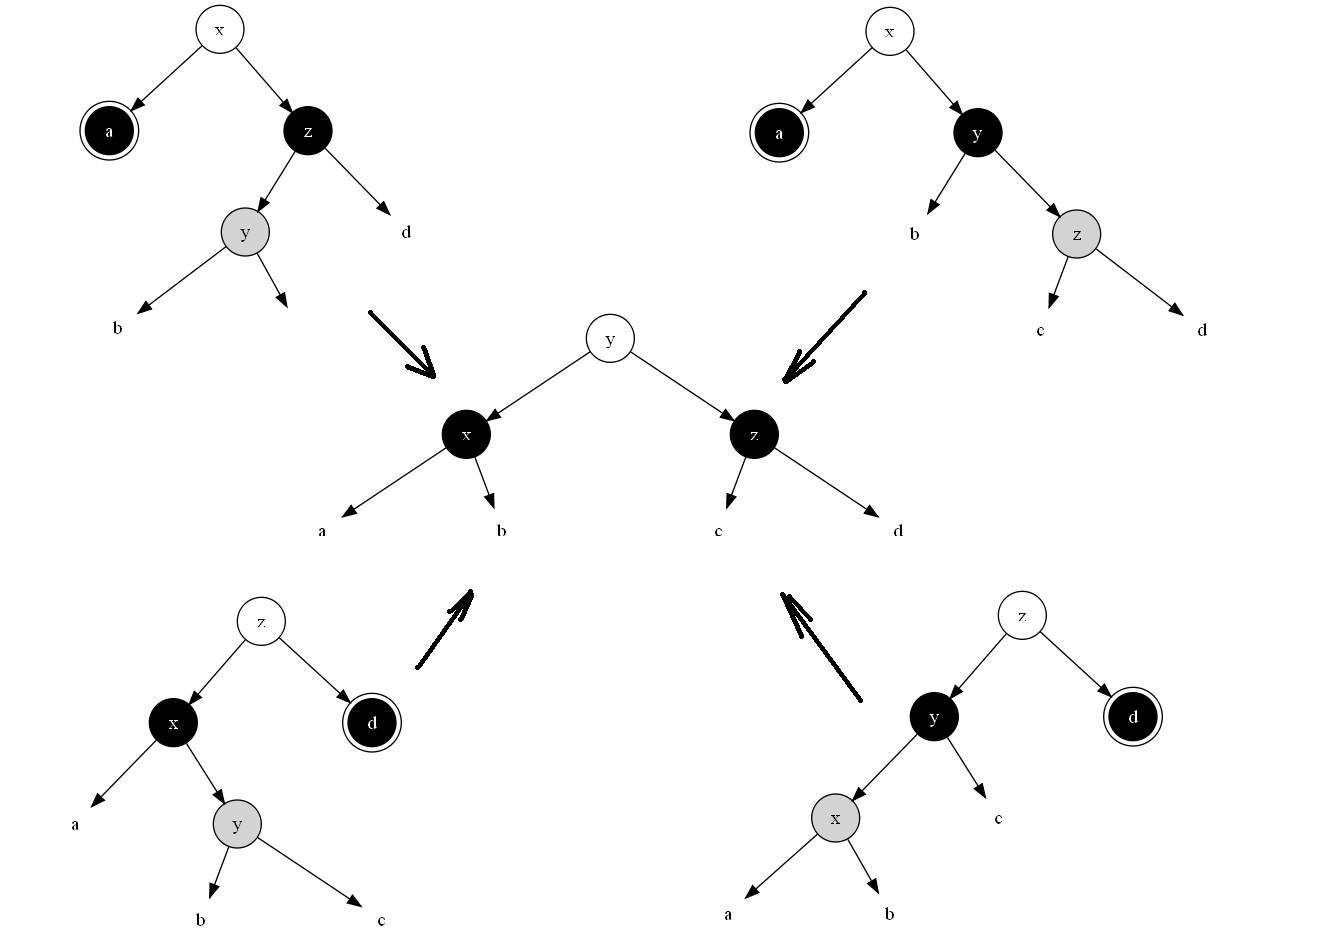
\includegraphics[scale=0.4]{img/del-case1.eps}
   \caption{双重黑色节点的兄弟节点为黑色,并且该兄弟节点有一个红色子节点。这种情况可以通过一次旋转操作来修复。}
   \label{fig:del-case1}
\end{figure}

我们可以在式(\ref{eq:db-nil})的基础上,增加这四种细分情况的处理:

\be
fixBlack^2(T) = \left \{
  \begin{array}
  {r@{\quad:\quad}l}
  ... & ... \\
  (\mathcal{C}, (\mathcal{B}, mkBlk(A), x, B), y, (\mathcal{B}, C, z, D)) & p 1.1 \\
  (\mathcal{C}, (\mathcal{B}, A, x, B), y, (\mathcal{B}, C, z, mkBlk(D))) & p 1.2 \\
  ... & ...
  \end{array}
\right .
\label{eq:db-case-1}
\ee

其中$p 1.1$和$p 1.2$各代表两种细分情况:

\[
p 1.1 : \left \{ \begin{array}{l}
  T = (\mathcal{C}, A, x, (\mathcal{B}, (\mathcal{R}, B, y, C), z, D)) \land color(A) = \mathcal{B}^2 \\
  \lor \\
  T = (\mathcal{C}, A, x, (\mathcal{B}, B, y, (\mathcal{R}, C, z, D))) \land color(A) = \mathcal{B}^2
  \end{array} \right \}
\]

\[
p 1.2 : \left \{ \begin{array}{l}
  T = (\mathcal{C}, (\mathcal{B}, A, x, (\mathcal{R}, B, y, C)), z, D) \land color(D) = \mathcal{B}^2 \\
  \lor \\
  T = (\mathcal{C}, (\mathcal{B}, (\mathcal{R}, A, x, B), y, C), z, D) \land color(D) = \mathcal{B}^2
  \end{array} \right \}
\]

除此之外,还有一种情况:不仅双重黑色节点的兄弟节点,该兄弟节点的两个子节点全部都是黑色。我们可以将这个兄弟节点染成红色,将双重黑色变回黑色,然后将双重黑色属性向上传递一层到父节点。如图\ref{fig:del-case2}所示,有两种对称的情况。

\begin{figure}[htbp]
  \centering
  \setlength{\unitlength}{1cm}
  \begin{picture}(10, 4)
  \put(5, 2){$\Rightarrow$}
  \subfloat[$x$的颜色为红或者黑。]{\includegraphics[scale=0.4]{img/case2-a.ps}}
  \subfloat[若$x$此前的颜色为红,将其变为黑色,否则变为双重黑色。]{\includegraphics[scale=0.4]{img/case2-a1.ps}}
  \end{picture}
  \\
  \begin{picture}(10, 5)
  \put(5, 2){$\Rightarrow$}
  \subfloat[$y$的颜色为红或者黑。]{\includegraphics[scale=0.4]{img/case2-b.ps}}
  \subfloat[若$y$此前的颜色为红,将其变为黑色,否则变为双重黑色。]{\includegraphics[scale=0.4]{img/case2-b1.ps}}
  \end{picture}
  \\
  \begin{picture}(1, 0.5)\end{picture} %pad
  \caption{将双重黑色向上传递。} \label{fig:del-case2}
\end{figure}

我们继续在式(\ref{eq:db-case-1})的基础上增加修复的定义。

\be
fixBlack^2(T) = \left \{
  \begin{array}
  {r@{\quad:\quad}l}
  ... & ... \\
  mkBlk((\mathcal{C}, mkBlk(A), x, (\mathcal{R}, B, y, C))) & p 2.1 \\
  mkBlk((\mathcal{C}, (\mathcal{R}, A, x, B), y, mkBlk(C))) & p 2.2 \\
  ... & ...
  \end{array}
\right .
\label{eq:db-case-2}
\ee

其中$p 2.1$和$p 2.2$定义如下:

\[
p 2.1 : \left \{ \begin{array}{l}
  T = (\mathcal{C}, A, x, (\mathcal{B}, B, y, C)) \land \\
  color(A) = \mathcal{B}^2 \land color(B) = color(C) = \mathcal{B}
  \end{array} \right \}
\]

\[
p 2.2 : \left \{ \begin{array}{l}
  T = (\mathcal{C}, (\mathcal{B}, A, x, B), y, C) \land \\
  color(C) = \mathcal{B}^2 \land color(A) = color(B) = \mathcal{B}
  \end{array} \right \}
\]

最后一个需要处理的情况是双重黑色节点的兄弟节点为红色。我们可以通过旋转,将其变换为$p 1.1$和$p 1.2$。如图\ref{fig:del-case2}所示。

\begin{figure}[htbp]
  \centering
  \includegraphics[scale=0.4]{img/del-case3.eps}
  \caption{双重黑色节点的兄弟节点为红色。} \label{fig:del-case3}
\end{figure}

在公式(\ref{eq:db-case-2})的基础上增加这一处理可以得到公式(\ref{eq:db-case-3})。

\be
fixBlack^2(T) = \left \{
  \begin{array}
  {r@{\quad:\quad}l}
  ... & ... \\
  fixBlack^2(\mathcal{B}, fixBlack^2((\mathcal{R}, A, x, B), y, C) & p 3.1 \\
  fixBlack^2(\mathcal{B}, A, x, fixBlack^2((\mathcal{R}, B, y, C)) & p 3.2 \\
  T & otherwise
  \end{array}
\right .
\label{eq:db-case-3}
\ee

其中$p 3.1$和$p 3.2$表示如下:

\[
p 3.1 : \{ color(T) = \mathcal{B} \land color(T_l) = \mathcal{B}^2 \land color(T_r) = \mathcal{R} \}
\]

\[
p 3.2 : \{ color(T) = \mathcal{B} \land color(T_l) = \mathcal{R} \land color(T_r) = \mathcal{B}^2 \}
\]


对于双重黑色全部情况的修复定义是一个递归函数。它有两个终止条件:一个是$p1.1$和$p1.2$,双重黑色节点被直接消除了;另外一个是将双重黑色继续向上传递,直到根节点。由于算法最终会将根节点染成黑色,所以双重黑色也会被消除。

综合公式(\ref{eq:db-nil})、(\ref{eq:db-case-1})、(\ref{eq:db-case-2})和(\ref{eq:db-case-3}),我们可以得到最终的Haskell删除程序。

\begin{lstlisting}
fixDB color BBEmpty k Empty = Node BB Empty k Empty
fixDB color BBEmpty k r = Node color Empty k r
fixDB color Empty k BBEmpty = Node BB Empty k Empty
fixDB color l k BBEmpty = Node color l k Empty
-- the sibling is black, and it has one red child
fixDB color a@(Node BB _ _ _) x (Node B (Node R b y c) z d) =
      Node color (Node B (makeBlack a) x b) y (Node B c z d)
fixDB color a@(Node BB _ _ _) x (Node B b y (Node R c z d)) =
      Node color (Node B (makeBlack a) x b) y (Node B c z d)
fixDB color (Node B a x (Node R b y c)) z d@(Node BB _ _ _) =
      Node color (Node B a x b) y (Node B c z (makeBlack d))
fixDB color (Node B (Node R a x b) y c) z d@(Node BB _ _ _) =
      Node color (Node B a x b) y (Node B c z (makeBlack d))
-- the sibling and its 2 children are all black, propagate the blackness up
fixDB color a@(Node BB _ _ _) x (Node B b@(Node B _ _ _) y c@(Node B _ _ _))
    = makeBlack (Node color (makeBlack a) x (Node R b y c))
fixDB color (Node B a@(Node B _ _ _) x b@(Node B _ _ _)) y c@(Node BB _ _ _)
    = makeBlack (Node color (Node R a x b) y (makeBlack c))
-- the sibling is red
fixDB B a@(Node BB _ _ _) x (Node R b y c) = fixDB B (fixDB R a x b) y c
fixDB B (Node R a x b) y c@(Node BB _ _ _) = fixDB B a x (fixDB R b y c)
-- otherwise
fixDB color l k r = Node color l k r
\end{lstlisting}

对于含有$n$个节点的红黑树,删除算法的复杂度为$O(\lg n)$。

\begin{Exercise}

\begin{itemize}
\item 选用一种编程语言,实现本节提到的“标记――重建”删除算法:也就是先将要删除的节点标记,但不进行真正的删除。当被标记的节点数目超过50\%的时候,用全部未标记的节点重建树。
\item 为什么不需要在$mkBlk$的调用处,显示地再调用$fixBlack^2$?
\end{itemize}

\end{Exercise}

\section{imperative的红黑树算法$\star$}
\index{红黑树!imperative插入}

通过归纳红,我们能够简洁地实现红黑树。作为对比,我们来看一下传统的imperative红黑树算法。

插入算法的基本思想仍然和二叉搜索树相同。此外,算法需要通过树的旋转操作修复平衡。

\begin{algorithmic}[1]
\Function{Insert}{$T, k$}
  \State $root \gets T$
  \State $x \gets$ \Call{Create-Leaf}{$k$}
  \State \Call{Color}{$x$} $\gets$ RED
  \State $p \gets$ NIL
  \While{$T \neq$ NIL}
    \State $p \gets T$
    \If{$k <$ \Call{Key}{$T$}}
      \State $T \gets $ \Call{Left}{$T$}
    \Else
      \State $T \gets $ \Call{Right}{$T$}
    \EndIf
  \EndWhile
  \State \Call{Parent}{$x$} $\gets p$
  \If{$p =$ NIL} \Comment{tree $T$ is empty}
    \State \Return $x$
  \ElsIf{$k <$ \Call{Key}{$p$}}
    \State \Call{Left}{$p$} $\gets x$
  \Else
    \State \Call{Right}{$p$} $\gets x$
  \EndIf
  \State \Return \Call{Insert-Fix}{$root, x$}
\EndFunction
\end{algorithmic}

在普通的二叉搜索树插入算法的基础上,当插入一个新节点时,我们将其染成红色。然后修复平衡并返回。上述算法可以转换为下面的Python例子程序\footnote{相应的C和C++语言的例子程序也可以同本书一并获得。}。

\lstset{language=Python}
\begin{lstlisting}
def rb_insert(t, key):
    root = t
    x = Node(key)
    parent = None
    while(t):
        parent = t
        if(key < t.key):
            t = t.left
        else:
            t = t.right
    if parent is None: #tree is empty
        root = x
    elif key < parent.key:
        parent.set_left(x)
    else:
        parent.set_right(x)
    return rb_insert_fix(root, x)
\end{lstlisting}

总共有3种基本情况需要修复。如果考虑左右对称,则需要修复6种情况。其中有两种可以合并。它们的父节点,以及父节点的兄弟节点均为红色。我们可以把它们变为黑色,然后把祖父节点染为红色。修复算法的实现如下:

\begin{algorithmic}[1]
\Function{Insert-Fix}{$T, x$}
  \While{\Call{Parent}{$x$} $\neq$ NIL $\land$ \textproc{Color}(\Call{Parent}{$x$}) = RED}
    \If{\textproc{Color}(\Call{Uncle}{$x$}) $=$ RED}
      \Comment{Case 1, x's uncle is red}
      \State \textproc{Color}(\Call{Parent}{$x$}) $\gets$ BLACK
      \State \textproc{Color}(\Call{Grand-Parent}{$x$}) $\gets$ RED
      \State \textproc{Color}(\Call{Uncle}{$x$}) $\gets$ BLACK
      \State $x \gets$ \Call{Grand-Parent}{$x$}
    \Else
      \Comment{x's uncle is black}
      \If{\Call{Parent}{$x$} = \textproc{Left}(\Call{Grand-Parent}{$x$})}
        \If{ $x =$ \textproc{Right}(\Call{Parent}{$x$})}
          \Comment{Case 2, x is a right child}
          \State $x \gets$ \Call{Parent}{$x$}
          \State $T \gets$ \Call{Left-Rotate}{$T, x$}
        \EndIf
        \Comment{Case 3, x is a left child}
        \State \textproc{Color}(\Call{Parent}{$x$}) $\gets$ BLACK
        \State \textproc{Color}(\Call{Grand-Parent}{$x$}) $\gets$ RED
        \State $T \gets$ \textproc{Right-Rotate}($T$, \Call{Grand-Parent}{$x$})
      \Else
         \If{ $x =$ \textproc{Left}(\Call{Parent}{$x$})}
          \Comment{Case 2, Symmetric}
          \State $x \gets$ \Call{Parent}{$x$}
          \State $T \gets$ \Call{Right-Rotate}{$T, x$}
        \EndIf
        \Comment{Case 3, Symmetric}
        \State \textproc{Color}(\Call{Parent}{$x$}) $\gets$ BLACK
        \State \textproc{Color}(\Call{Grand-Parent}{$x$}) $\gets$ RED
        \State $T \gets$ \textproc{Left-Rotate}($T$, \Call{Grand-Parent}{$x$})
      \EndIf
    \EndIf
  \EndWhile
  \State \Call{Color}{$T$} $\gets$ BLACK
  \State \Return $T$
\EndFunction
\end{algorithmic}

这一算法向红黑树种插入key的复杂度为$O(\lg n)$。和前面定义的$balance$函数相比,我们可以发现它们的差异。两种方法不仅仅在篇幅长短上不同,具体的逻辑也不一样。即使输入同一组key的序列,两种方法会也构造出不同的红黑树。使用模式匹配的算法存在一些性能上的损失。Okasaki在\cite{okasaki}中给出了详细的解释。

上述修复算法可以实现为如下的Python例子程序。

\begin{lstlisting}
# Fix the red->red violation
def rb_insert_fix(t, x):
    while(x.parent and x.parent.color==RED):
        if x.uncle().color == RED:
            #case 1: ((a:R x:R b) y:B c:R) ==> ((a:R x:B b) y:R c:B)
            set_color([x.parent, x.grandparent(), x.uncle()],
                      [BLACK, RED, BLACK])
            x = x.grandparent()
        else:
            if x.parent == x.grandparent().left:
                if x == x.parent.right:
                    #case 2: ((a x:R b:R) y:B c) ==> case 3
                    x = x.parent
                    t=left_rotate(t, x)
                # case 3: ((a:R x:R b) y:B c) ==> (a:R x:B (b y:R c))
                set_color([x.parent, x.grandparent()], [BLACK, RED])
                t=right_rotate(t, x.grandparent())
            else:
                if x == x.parent.left:
                    #case 2': (a x:B (b:R y:R c)) ==> case 3'
                    x = x.parent
                    t = right_rotate(t, x)
                # case 3': (a x:B (b y:R c:R)) ==> ((a x:R b) y:B c:R)
                set_color([x.parent, x.grandparent()], [BLACK, RED])
                t=left_rotate(t, x.grandparent())
    t.color = BLACK
    return t
\end{lstlisting}

图\ref{fig:imperative-insert}给出了两棵红黑树,它们是使用和图\ref{fig:insert-example}中完全相同的序列构造出的。我们可以发现它们明显不同。

\begin{figure}[htbp]
   \centering
   \subfloat[]{\includegraphics[scale=0.4]{img/clrs-fig-13-4.ps}}
   \subfloat[]{\includegraphics[scale=0.4]{img/python-insert.ps}}
   \caption{Imperative算法构建出的红黑树。}
   \label{fig:imperative-insert}
\end{figure}

红黑树的imperative删除算法更加复杂,我们不再给出。作为练习,读者可以通过树的旋转,尝试实现红黑树的删除算法。

\begin{Exercise}

\begin{itemize}
\item 使用一种imperative编程语言实现红黑树的删除算法。可以参考\cite{CLRS}中给出的不同情况。
\end{itemize}

\end{Exercise}

\section{其它}
红黑树是最广泛使用的一种平衡二叉搜索树。另外一种自平衡二叉树是AVL树,我们将在下一章介绍。红黑树可以帮助我们了解其它更复杂的数据结构。如果我们将子节点的数目从两个扩展到$k$个,并且保持树的平衡,就可以演化到B树。如果我们在边上,而非在节点上存储数据,我们就得到了Trie。由于常见红黑树算法需要处理很多情况,代码篇幅较长,很多初学者会感觉红黑树很复杂。

Okasaki的工作使得红黑树算法变得容易理解。这激发了很多其它程序设计语言进行了类似的实现\cite{rosetta}。本书中给出的Splay树、AVL树等算法实现也是受到这一启发而完成的。

\begin{thebibliography}{99}

\bibitem{CLRS}
Thomas H. Cormen, Charles E. Leiserson, Ronald L. Rivest and Clifford Stein.
``Introduction to Algorithms, Second Edition''. ISBN:0262032937. The MIT Press. 2001 (《算法导论》中文版)

\bibitem{okasaki}
Chris Okasaki. ``FUNCTIONAL PEARLS Red-Black Trees in a Functional Setting''. J. Functional Programming. 1998

\bibitem{okasaki-blog}
Chris Okasaki. ``Ten Years of Purely Functional Data Structures''. http://okasaki.blogspot.com/2008/02/ten-years-of-purely-functional-data.html

\bibitem{wiki}
Wikipedia. ``Red-black tree''. http://en.wikipedia.org/wiki/Red-black\_tree

\bibitem{lyn}
Lyn Turbak. ``Red-Black Trees''. cs.wellesley.edu/~cs231/fall01/red-black.pdf Nov. 2, 2001.

\bibitem{sgi-stl}
SGI STL. http://www.sgi.com/tech/stl/

\bibitem{rosetta}
Pattern matching. http://rosettacode.org/wiki/Pattern\_matching

\end{thebibliography}

\ifx\wholebook\relax\else
\end{document}
\fi


\ifx\wholebook\relax \else
% ------------------------

\documentclass[UTF8]{article}
%------------------- Other types of document example ------------------------
%
%\documentclass[twocolumn]{IEEEtran-new}
%\documentclass[12pt,twoside,draft]{IEEEtran}
%\documentstyle[9pt,twocolumn,technote,twoside]{IEEEtran}
%
%-----------------------------------------------------------------------------
%
% loading packages
%

\RequirePackage{ifpdf}
\RequirePackage{ifxetex}

%
%
\ifpdf
  \RequirePackage[pdftex,%
       bookmarksnumbered,%
              colorlinks,%
          linkcolor=blue,%
              hyperindex,%
        plainpages=false,%
       pdfstartview=FitH]{hyperref}
\else\ifxetex
  \RequirePackage[bookmarksnumbered,%
               colorlinks,%
           linkcolor=blue,%
               hyperindex,%
         plainpages=false,%
        pdfstartview=FitH]{hyperref}
\else
  \RequirePackage[dvipdfm,%
        bookmarksnumbered,%
               colorlinks,%
           linkcolor=blue,%
               hyperindex,%
         plainpages=false,%
        pdfstartview=FitH]{hyperref}
\fi\fi
%\usepackage{hyperref}

% other packages
%--------------------------------------------------------------------------
\usepackage{graphicx, color}
\usepackage{subfig}
\usepackage{tikz}
\usetikzlibrary{matrix,positioning}

\usepackage{amsmath, amsthm, amssymb} % for math
\usepackage{exercise} % for exercise
\usepackage{import} % for nested input

%
% for programming
%
\usepackage{verbatim}
\usepackage{listings}
%\usepackage{algorithmic} %old version; we can use algorithmicx instead
\usepackage{algorithm}
\usepackage[noend]{algpseudocode} %for pseudo code, include algorithmicsx automatically
\usepackage{appendix}
\usepackage{makeidx} % for index support
\usepackage{titlesec}

\usepackage[cm-default]{fontspec}
\usepackage{xunicode}

% detect and select Chinese font
% ------------------------------
% the following cmd can list all availabe Chinese fonts in host.
% fc-list :lang=zh
\def\myfont{STHeiti}  % Under Mac OS X
\def\linuxfallback{WenQuanYi Micro Hei} % Under Linux
\def\winfallback{SimSun} % Under Windows
\suppressfontnotfounderror1 % Avoid setting exit code (error level) to break make process
\count255=\interactionmode
\batchmode
\font\foo="\myfont"\space at 10pt
\ifx\foo\nullfont
  \font\foo = "\linuxfallback"\space at 10pt
  \ifx\foo\nullfont
    \font\foo = "\winfallback"\space at 10pt
    \ifx\foo\nullfont
      \errorstopmode
      \errmessage{no suitable Chinese font found}
    \else
      \let\myfont=\winfallback % Windows
    \fi
  \else
    \let\myfont=\linuxfallback % Linux
  \fi
\fi
\interactionmode=\count255
\setmainfont[Mapping=tex-text]{\myfont}

\XeTeXlinebreaklocale "zh"  % to solve the line breaking issue
\XeTeXlinebreakskip = 0pt plus 1pt minus 0.1pt

\titleformat{\paragraph}
{\normalfont\normalsize\bfseries}{\theparagraph}{1em}{}
\titlespacing*{\paragraph}
{0pt}{3.25ex plus 1ex minus .2ex}{1.5ex plus .2ex}

\lstdefinelanguage{Smalltalk}{
  morekeywords={self,super,true,false,nil,thisContext}, % This is overkill
  morestring=[d]',
  morecomment=[s]{"}{"},
  alsoletter={\#:},
  escapechar={!},
  literate=
    {BANG}{!}1
    {UNDERSCORE}{\_}1
    {\\st}{Smalltalk}9 % convenience -- in case \st occurs in code
    % {'}{{\textquotesingle}}1 % replaced by upquote=true in \lstset
    {_}{{$\leftarrow$}}1
    {>>>}{{\sep}}1
    {^}{{$\uparrow$}}1
    {~}{{$\sim$}}1
    {-}{{\sf -\hspace{-0.13em}-}}1  % the goal is to make - the same width as +
    %{+}{\raisebox{0.08ex}{+}}1		% and to raise + off the baseline to match -
    {-->}{{\quad$\longrightarrow$\quad}}3
	, % Don't forget the comma at the end!
  tabsize=2
}[keywords,comments,strings]

% for better Haskell code outlook
\lstdefinelanguage{Haskell}{
  basicstyle=\small\ttfamily,
  flexiblecolumns=false,
  basewidth={0.5em,0.45em},
  literate={+}{{$+$}}1 {/}{{$/$}}1 {*}{{$*$}}1 {=}{{$=$}}1
           {>}{{$>$}}1 {<}{{$<$}}1 {\\}{{$\lambda$}}1
           {\\\\}{{\char`\\\char`\\}}1
           {->}{{$\rightarrow$}}2 {>=}{{$\geq$}}2 {<-}{{$\leftarrow$}}2
           {<=}{{$\leq$}}2 {=>}{{$\Rightarrow$}}2
           {\ .}{{$\circ$}}2 {\ .\ }{{$\circ$}}2
           {>>}{{>>}}2 {>>=}{{>>=}}2
           {|}{{$\mid$}}1
}[keywords,comments,strings]

\lstloadlanguages{C, C++, Lisp, Haskell, Python, Smalltalk}

\lstset{
  showstringspaces = false
}

% ======================================================================

\def\BibTeX{{\rm B\kern-.05em{\sc i\kern-.025em b}\kern-.08em
    T\kern-.1667em\lower.7ex\hbox{E}\kern-.125emX}}

%
% mathematics
%
\newcommand{\be}{\begin{equation}}
\newcommand{\ee}{\end{equation}}
\newcommand{\bmat}[1]{\left( \begin{array}{#1} }
\newcommand{\emat}{\end{array} \right) }
\newcommand{\VEC}[1]{\mbox{\boldmath $#1$}}

% numbered equation array
\newcommand{\bea}{\begin{eqnarray}}
\newcommand{\eea}{\end{eqnarray}}

% equation array not numbered
\newcommand{\bean}{\begin{eqnarray*}}
\newcommand{\eean}{\end{eqnarray*}}

\newtheorem{theorem}{Theorem}[section]
\newtheorem{lemma}[theorem]{Lemma}
\newtheorem{proposition}[theorem]{Proposition}
\newtheorem{corollary}[theorem]{Corollary}


\setcounter{page}{1}

\begin{document}

%--------------------------

% ================================================================
%                 COVER PAGE
% ================================================================

\title{AVL树}

\author{刘新宇
\thanks{{\bfseries 刘新宇} \newline
  Email: liuxinyu95@gmail.com \newline}
  }

\maketitle
\fi

\markboth{AVL树}{初等算法}

\ifx\wholebook\relax
\chapter{AVL树}
\numberwithin{Exercise}{chapter}
\fi

% ================================================================
%                 Introduction
% ================================================================
\section{简介}
\label{introduction} \index{AVL树}

\subsection{度量树的平衡性}

除了红黑树,还有没有其他自平衡二叉树呢?为了度量一棵二叉树的平衡,我们可以比较它左右分支的高度差,如果差很大,则说明树不平衡。定义一棵树的高度差如下:

\be
  \delta(T) = |L| - |R|
\ee

其中$|T|$代表树$T$的高度,$L$和$R$分别代表左右分支。

若$\delta(T) = 0$,说明树是平衡的。例如,一个高度为$h$的完全二叉树有$n = 2^h-1$个节点。除了叶子节点外,所有节点都含有两个非空的分支。完全二叉树就满足$\delta(T)=0$。另外一个特殊的例子是空树:$\delta(\phi) = 0$。通常$\delta(T)$的绝对值越小,说明树越平衡。

我们定义$\delta(T)$为一棵二叉树的\underline{平衡因子}。

% ================================================================
% Definition
% ================================================================
\section{AVL树的定义}
\index{AVL树!定义}

如果一棵二叉搜索树的所有子树都满足如下条件,我们称之为AVL树。

\be
  |\delta(T)| \leq 1
\ee

AVL树中所有子树平衡因子的绝对值都不大于1,只可能是-1、0,或1这三个值。图\ref{fig:avl-example}给出了一个AVL树的例子。

\begin{figure}[htbp]
   \centering
   \includegraphics[scale=0.5]{img/avl-example.ps}
   \caption{AVL树的例子} \label{fig:avl-example}
\end{figure}

为什么AVL树能保证树的平衡性呢?或者说为什么这个定义能保证一棵有$n$个节点的树的高度为$O(\lg n)$?我们可以用下面的方法来证明这一事实。

对于一棵高为$h$的AVL树,它的节点数目并不是一个固定的值。当它是一棵完全二叉树时,含有的节点数目最多,为$2^h-1$。那么它最少包含多少节点呢?我们记函数$N(h)$代表高度为$h$时,AVL树含有最少的节点数。对于简单的情况,我们可以立即给出$N(h)$的值:

\begin{itemize}
\item 空树,$h=0$,$N(0)=0$;
\item 只有一个根节点的树,$h=1$,$N(1)=1$;
\end{itemize}

一般情况下$N(h)$是怎样的呢?图\ref{fig:N-h-relation}中给出了一个高度为$h$的AVL树$T$。它包含三部份:根节点和左右两个分支$L$与$R$。树的高度和子树高度之间满足下面的关系:

\be
  h= max(|L|, |R|) + 1
\ee

因此,必然存在一个子树的高度为$h-1$。根据AVL树的定义,我们有 $||L| -|R|| \leq 1$。所以另外一棵子树的高度不会小于$h-2$。而$T$所包含的节点数为两个子树的节点数再加1(1个根节点)。于是我们得到下面的递归关系:

\be
  N(h) = N(h-1) + N(h-2) + 1
  \label{eq:Fibonacci-like}
\ee

\begin{figure}[htbp]
   \centering
   \includegraphics[scale=0.5]{img/Nh-lvr.ps}
   \caption{高度为$h$的AVL树,其中一个分支为$h-1$,另外一个分支的高度不小于$h-2$} \label{fig:N-h-relation}
\end{figure}

这一递归形式让我们联想起著名的斐波那契(Fibonacci)数列。如果定义$N'(h) = N(h)+1$,我们就可以将(\ref{eq:Fibonacci-like})转换成斐波那契数列。

\be
  N'(h) = N'(h-1) + N'(h-2)
\ee

\begin{lemma}
\label{lemma:N-phi}
定理:若$N(h)$表示高为$h$的AVL树的节点数目最小值,令$N'(h) = N(h) + 1$,则:

\be
  N'(h) \geq \phi^h
\ee

其中$\phi = \frac{\sqrt{5}+1}{2}$,通常被称为黄金分割比。
\end{lemma}

\begin{proof}
证明:使用数学归纳法。对于起始情况,我们有:
\begin{itemize}
\item $h=0$, $N'(0) = 1 \geq \phi^0 = 1$
\item $h=1$, $N'(1) = 2 \geq \phi^1 = 1.618...$
\end{itemize}

对于递推情况,设$N'(h) \geq \phi^h$。
\[
  \begin{array}{lll}
  N'(h+1) & = N'(h) + N'(h-1) & \{Fibonacci\} \\
          & \geq \phi^h + \phi^{h-1} & \\
          & = \phi^{h-1}(\phi + 1) & \{\phi + 1 = \phi^2 = \frac{\sqrt{5}+3}{2}\} \\
          & = \phi^{h+1}
 \end{array}
\]
\end{proof}

由定理\ref{lemma:N-phi},我们立即得到下面的结果:

\be
  h \leq log_{\phi}(n+1) = log_{\phi}(2) \cdot \lg (n+1) \approx 1.44 \lg (n+1)
  \label{eq:AVL-height}
\ee

这一不等式说明AVL树的高度为$O(\lg n)$,从而保证了平衡性。

在树的基本操作中,插入和删除会改变树的结构。如果由此导致平衡因子的绝对值超过1,就需要通过修复使得$|\delta|$恢复到1以内。常见的修复方法是使用树旋转。受到Okasaki在红黑树\cite{okasaki}中的思路启发,本章中,我们介绍一种模式匹配(pattern matching)方法。这种“改变―恢复”的操作,使得AVL树成为了一种自平衡二叉树。作为比较,本章同样也给出命令式的AVL树算法。

平衡因子$\delta$显然可以通过递归求出。另外一种方法是在每个节点中保存一分平衡因子的值,如果树被改变,我们只要更新这个值就可以了。这一方法不需要每次都计算。

根据这一思路,我们在二叉搜索树的定义中增加一个$\delta$变量,如下面的C++代码所示\footnote{有些实现不保存$\delta$,取而代之保存树的高度,如\cite{py-avl}。}。

\lstset{language=C++}
\begin{lstlisting}
template <class T>
struct node{
  int delta;
  T key;
  node* left;
  node* right;
  node* parent;
};
\end{lstlisting}

某些纯函数式实现使用不同的constructor来保存平衡因子$\delta$。例如在\cite{hackage}中,定义了4个不同的constructor:\texttt{E}、\texttt{N}、\texttt{P}、\texttt{Z}。其中,\texttt{E}代表空树$\phi$;\texttt{N}代表平衡因子为-1;\texttt{P}代表平衡因子为1;\texttt{Z}代表平衡因子为0。

本章中,我们直接在节点中保存平衡因子的值。

\lstset{language=Haskell}
\begin{lstlisting}
data AVLTree a = Empty
               | Br (AVLTree a) a (AVLTree a) Int
\end{lstlisting}

不改变树的操作,包括查找,寻找最大、最小值和二叉搜索树完全一样。我们略过它们,仅仅关注哪些会改变树结构的操作。

% ================================================================
%                 Insertion
% ================================================================
\section{插入}
\index{AVL树!插入}

在AVL树中插入一个新元素可能造成AVL树的平衡性被破坏,平衡因子$\delta$的绝对值有可能超过1。为了恢复平衡,可以根据不同的插入情形进行树的旋转操作。大多数命令式实现采用这种方法。

另外一种方法很像Okasaki在红黑树实现中使用的模式匹配方法。它的特点是简单直观。

向AVL树中插入一个新key,根节点的平衡因子的\underline{变化}会在$[-1, 1]$之间\footnote{注意:这里不是说平衡因子的值在$[-1, 1]$内,而是说它的变化在这个范围内。},树的高度最多增加1。我们需要递归地使用这一信息来更新其他层级上的平衡因子$\delta$。定义插入算法的结果为一对值$(T', \Delta H)$,其中$T'$为插入后的新树,$\Delta H$为树高度的增加值。令函数$first(pair)$可以取得一对值中的第一个元素。我们可以在二叉搜索树的插入算法上进行改动,定义AVL树的插入操作:

\be
insert(T, k) = first(ins(T, k))
\ee

其中

\be
ins(T, k) = \left \{
  \begin{array}
  {r@{\quad:\quad}l}
  ((\phi, k, \phi, 0), 1) & T = \phi \\
  tree(ins(L, k), k', (R, 0), \Delta) & k < k' \\
  tree((L, 0), k', ins(R, k), \Delta) & otherwise
  \end{array}
\right.
\label{eq:ins}
\ee

$L$、$R$、$k'$、$\Delta$的定义如下,它们分别表示左右子树,key和平衡因子。

\[
  \begin{array}{l}
  L = left(T) \\
  R = right(T) \\
  k' = key(T) \\
  \Delta = \delta(T)
  \end{array}
\]

向AVL树$T$中插入一个新key $k$时,如果树为空,结果为一个叶子节点,节点的key为$k$,平衡因子为0。树的高度增加1。

否则,如果$T$不为空,我们需要比较根节点的key k'和待插入key k的大小。如果$k$小于根节点的key,我们将其递归插入左子树,否则将其插入右子树。

As we defined above, the result of the recursive insertion is a
pair like $(L', \Delta H_l)$, we need do balancing adjustment as well
as updating the increment of height. Function $tree()$ is defined
to dealing with this task. It takes 4 parameters as $(L', \Delta H_l)$,
$Key$, $(R', \Delta H_r)$, and $\Delta$. The result of this function
is defined as $(T', \Delta H)$, where $T'$ is the new tree after
adjustment, and $\Delta H$ is the new increment of height which is
defined as

\be
  \Delta H = |T'| - |T|
\ee

This can be further detailed deduced in 4 cases.

\be
\begin{array}{rl}
  \Delta H & = |T'| - |T| \\
              & = 1 + max(|R'|, |L'|) - (1 + max(|R|, |L|)) \\
              & = max(|R'|, |L'|) - max(|R|, |L|) \\
              & = \left \{
                  \begin{array}{r@{\quad:\quad}l}
                  \Delta H_r & \Delta \geq 0 \land \Delta' \geq 0 \\
                  \Delta + \Delta H_r & \Delta \leq 0 \land \Delta' \geq 0 \\
                  \Delta H_l - \Delta & \Delta \geq 0 \land \Delta' \leq 0 \\
                  \Delta H_l & otherwise
                  \end{array} \right .
\end{array}
\ee

To prove this equation, note the fact that the height can't increase
both in left and right with only one insertion.

These 4 cases can be explained from the definition of balance factor
definition that it equal to the difference from the right sub tree
and left sub tree.

\begin{itemize}
\item If $\Delta \geq 0$ and $\Delta' \geq 0$, it means that the height
of right sub tree isn't less than the height of left sub tree both
before insertion and after insertion. In this case, the increment in
height of the tree is only `contributed' from the right sub tree, which
is $\Delta H_r$.

\item If $\Delta \leq 0$, which means the height of left sub tree isn't
less than the height of right sub tree before, and it becomes
$\Delta' \geq 0$,
which means that the height of right sub tree increases due to insertion,
and the left side keeps same ($|L'|=|L|$). So the increment in height is
\[
\begin{array}{rll}
\Delta H & = max(|R'|, |L'|) - max (|R|, |L|) & \{\Delta \leq 0 \land \Delta' \geq 0 \}\\
         & = |R'|-|L'| & \{|L|=|L'| \}\\
         & = |R|+\Delta H_r - |L| & \\
         & = \Delta + \Delta H_r &
\end{array}
\]

\item For the case $\Delta \geq 0 \land \Delta' \leq 0$, Similar as the
second one, we can get.

\[
\begin{array}{rll}
\Delta H & = max(|R'|, |L'|) - max (|R|, |L|) & \{\Delta \geq 0 \land \Delta' \leq 0 \}\\
         & = |L'|-|R| & \\
         & = |L|+\Delta H_l - |R| & \\
         & = \Delta H_l - \Delta&
\end{array}
\]

\item For the last case, the both $\Delta$ and $\Delta'$ is no bigger than
zero, which means the height left sub tree is always greater than or equal
 to the right sub tree, so the increment in height is only `contributed'
from the right sub tree, which is $\Delta H_l$.
\end{itemize}

The next problem in front of us is how to determine the new balancing
factor value $\Delta'$ before performing balancing adjustment.
According to the definition of AVL tree, the balancing factor is the
height of right sub tree minus the height of left sub tree. We have
the following facts.

\be
\begin{array}{rl}
\Delta' & = |R'| - |L'| \\
        & = |R| + \Delta H_r - (|L| + \Delta H_l) \\
        & = |R| - |L| + \Delta H_r - \Delta H_l \\
        & = \Delta + \Delta H_r - \Delta H_l
\end{array}
\ee

With all these changes in height and balancing factor get clear, it's
possible to define the $tree()$ function mentioned in (\ref{eq:ins}).

\be
tree((L', \Delta H_l), Key, (R', \Delta H_r), \Delta) =
  balance (node(L', Key, R', \Delta'), \Delta H)
\ee

Before we moving into details of balancing adjustment, let's translate
the above equations to real programs in Haskell.

First is the insert function.

\lstset{language=Haskell}
\begin{lstlisting}
insert::(Ord a)=>AVLTree a -> a -> AVLTree a
insert t x = fst $ ins t where
    ins Empty = (Br Empty x Empty 0, 1)
    ins (Br l k r d)
        | x < k     = tree (ins l) k (r, 0) d
        | x == k    = (Br l k r d, 0)
        | otherwise = tree (l, 0) k (ins r) d
\end{lstlisting} %$

Here we also handle the case that inserting a duplicated key (which
means the key has already existed.) as just overwriting.

\begin{lstlisting}
tree::(AVLTree a, Int) -> a -> (AVLTree a, Int) -> Int -> (AVLTree a, Int)
tree (l, dl) k (r, dr) d = balance (Br l k r d', delta) where
    d' = d + dr - dl
    delta = deltaH d d' dl dr
\end{lstlisting}

And the definition of height increment is as below.

\begin{lstlisting}
deltaH :: Int -> Int -> Int -> Int -> Int
deltaH d d' dl dr
       | d >=0 && d' >=0 = dr
       | d <=0 && d' >=0 = d+dr
       | d >=0 && d' <=0 = dl - d
       | otherwise = dl
\end{lstlisting}

\subsection{Balancing adjustment}
\index{AVL tree!balancing}
As the pattern matching approach is adopted in doing re-balancing.
We need consider what kind of patterns violate the AVL tree property.

Figure \ref{fig:insert-fix} shows the 4 cases which need fix. For all
these 4 cases the balancing factors are either -2, or +2 which exceed
the range of $[-1, 1]$. After balancing adjustment, this factor turns
to be 0, which means the height of left sub tree is equal to the right
sub tree.

\begin{figure}[htbp]
   \begin{center}
     \setlength{\unitlength}{1cm}
     \begin{picture}(15, 15)
        % arrows
        \put(4.5, 9.5){\vector(1, -1){1}}
        \put(4.5, 5){\vector(1, 1){1}}
        \put(10, 9.5){\vector(-1, -1){1}}
        \put(10, 5){\vector(-1, 1){1}}
        % delta values
        \put(5, 13){$\delta(z) = -2$}
        \put(2.5, 12){$\delta(y) = -1$}
        \put(10, 13){$\delta(x) = 2$}
        \put(11.5, 11.5){$\delta(y) = 1$}
        \put(1.5, 5.5){$\delta(z) = -2$}
        \put(3.5, 4){$\delta(x) = 1$}
        \put(12, 5.5){$\delta(x) = 2$}
        \put(10.5, 4){$\delta(z) = -1$}
        \put(7.5, 10){$\delta'(y) = 0$}
        % graphics
	\put(0, 7){\includegraphics[scale=0.5]{img/insert-ll.ps}}
        \put(0, 0){\includegraphics[scale=0.5]{img/insert-lr.ps}}
        \put(7, 7){\includegraphics[scale=0.5]{img/insert-rr.ps}}
        \put(8.5, 0){\includegraphics[scale=0.5]{img/insert-rl.ps}}
        \put(2, 5){\includegraphics[scale=0.5]{img/insert-fixed.ps}}
      \end{picture}
     \caption{4 cases for balancing a AVL tree after insertion} \label{fig:insert-fix}
  \end{center}
\end{figure}

We call these four cases left-left lean, right-right lean, right-left lean,
and left-right lean cases in clock-wise direction from top-left. We denote
the balancing factor before fixing as $\delta(x), \delta(y)$, and $\delta(z)$, while after fixing, they changes to $\delta'(x), \delta'(y)$, and
$\delta'(z)$ respectively.

We'll next prove that, after fixing, we have $\delta(y)=0$ for all
four cases, and we'll provide the result values of $\delta'(x)$ and
$\delta'(z)$.

\subsubsection*{Left-left lean case}

As the structure of sub tree $x$ doesn't change due to fixing, we immediately get
$\delta'(x) = \delta(x)$.

Since $\delta(y) = -1$ and $\delta(z) = -2$, we have

\be
  \begin{array}{l}
  \delta(y) = |C| - |x| = -1 \Rightarrow |C| = |x| - 1 \\
  \delta(z) = |D| - |y| = -2 \Rightarrow |D| = |y| - 2
  \end{array}
  \label{eq:ll-cd}
\ee

After fixing.

\be
  \begin{array}{rll}
  \delta'(z) & = |D| - |C| & \{ From (\ref{eq:ll-cd}) \}\\
             & = |y| - 2 - (|x| - 1) & \\
             & = |y| - |x| - 1 & \{  x \text{ is child of } y \Rightarrow |y|-|x| = 1\} \\
             & = 0 &
  \end{array}
  \label{eq:ll-delta-z}
\ee

For $\delta'(y)$, we have the following fact after fixing.

\be
  \begin{array}{rll}
  \delta'(y) & = |z| - |x| & \\
             & = 1 + max(|C|, |D|) - |x| & \{ \text{By (\ref{eq:ll-delta-z}), we have} |C| = |D|\} \\
             & = 1 + |C| - |x| & \{ \text{By (\ref{eq:ll-cd})}\} \\
             & = 1 + |x| - 1 - |x| & \\
             & = 0 &
  \end{array}
\ee

Summarize the above results, the left-left lean case adjust the balancing
factors as the following.

\be
  \begin{array}{l}
  \delta'(x) = \delta(x) \\
  \delta'(y) = 0 \\
  \delta'(z) = 0
  \end{array}
\ee

\subsubsection*{Right-right lean case}

Since right-right case is symmetric to left-left case, we can easily achieve the result balancing factors as

\be
  \begin{array}{l}
  \delta'(x) = 0 \\
  \delta'(y) = 0 \\
  \delta'(z) = \delta(z)
  \end{array}
  \label{eq:rr-result}
\ee

\subsubsection*{Right-left lean case}

First let's consider $\delta'(x)$. After balance fixing, we have.

\be
  \delta'(x) = |B| - |A|
  \label{eq:rl-dx}
\ee

Before fixing, if we calculate the height of $z$, we can get.

\be
  \begin{array}{rll}
  |z| & = 1 + max(|y|, |D|) &  \{ \delta(z) = -1 \Rightarrow |y| > |D|\} \\
      & = 1 + |y| & \\
      & = 2 + max(|B|, |C|)
  \end{array}
  \label{eq:rl-z}
\ee

While since $\delta(x) = 2$, we can deduce that.

\be
  \begin{array}{rll}
  \delta(x) = 2 & \Rightarrow |z| - |A| = 2 & \{ \text{By (\ref{eq:rl-z})} \}\\
                & \Rightarrow 2 + max(|B|, |C|) - |A| = 2 & \\
                & \Rightarrow max(|B|, |C|) - |A| = 0 &
  \end{array}
  \label{eq:rl-ca}
\ee

If $\delta(y) = 1$, which means $|C| - |B| = 1$, it means

\be
  max(|B|, |C|)= |C| = |B|+1
\ee

Take this into (\ref{eq:rl-ca}) yields

\be
  \begin{array}{ll}
  |B|+1-|A| = 0 \Rightarrow |B|-|A|= -1 & \{ \text{By (\ref{eq:rl-dx}) } \} \\
  \Rightarrow \delta'(x) = -1 &
  \end{array}
\ee

If $\delta(y) \neq 1$, it means $max(|B|, |C|) = |B|$, taking this into
(\ref{eq:rl-ca}), yields.

\be
  \begin{array}{ll}
  |B| - |A| = 0  & \{ \text{By (\ref{eq:rl-dx})} \} \\
  \Rightarrow \delta'(x) = 0 &
  \end{array}
\ee

Summarize these 2 cases, we get relationship of $\delta'(x)$ and
$\delta(y)$ as the following.

\be
\delta'(x) = \left \{
  \begin{array}
  {r@{\quad:\quad}l}
  -1 & \delta(y) = 1 \\
  0 & otherwise
  \end{array}
\right.
\label{eq:rl-dx-dy}
\ee

For $\delta'(z)$ according to definition, it is equal to.

\be
  \begin{array}{rll}
    \delta'(z) & = |D| - |C| & \{ \delta(z) = -1 = |D| - |y| \} \\
               & = |y| - |C| - 1 & \{ |y| = 1 + max(|B|, |C|) \} \\
               & = max(|B|, |C|) - |C|
  \end{array}
  \label{eq:rl-dz}
\ee

If $\delta(y) = -1$, then we have $|C| - |B| = -1$, so $max(|B|, |C|) = |B| = |C| + 1$. Takes this into (\ref{eq:rl-dz}), we get $\delta'(z) = 1$.

If $\delta(y) \neq -1$, then $max(|B|, |C|) = |C|$, we get $\delta'(z)=0$.

Combined these two cases, the relationship between $\delta'(z)$ and $\delta(y)$ is as below.

\be
\delta'(z) = \left \{
  \begin{array}
  {r@{\quad:\quad}l}
  1 & \delta(y) = -1 \\
  0 & otherwise
  \end{array}
  \right.
  \label{eq:rl-dz-dy}
\ee

Finally, for $\delta'(y)$, we deduce it like below.

\be
  \begin{array}{rl}
  \delta'(y) & = |z| - |x| \\
             & = max(|C|, |D|) - max(|A|, |B|)
  \end{array}
  \label{eq:rl-dy}
\ee

There are three cases.
\begin{itemize}

\item If $\delta(y)=0$, it means $|B|=|C|$, and according to (\ref{eq:rl-dx-dy}) and (\ref{eq:rl-dz-dy}), we have $\delta'(x)=0 \Rightarrow |A| = |B|$, and $\delta'(z)=0 \Rightarrow |C|=|D|$, these lead to $\delta'(y)=0$.

\item If $\delta(y)=1$, From (\ref{eq:rl-dz-dy}), we have $\delta'(z)=0 \Rightarrow |C| = |D|$.
\[
  \begin{array}{rll}
  \delta'(y) & = max(|C|, |D|) - max(|A|, |B|) & \{|C|=|D|\} \\
             & = |C| - max(|A|, |B|) & \{\text{From (\ref{eq:rl-dx-dy}): $\delta'(x)=-1 \Rightarrow |B|-|A|=-1$} \} \\
             & = |C| - (|B| + 1) & \{ \delta(y) = 1 \Rightarrow |C|-|B|=1\} \\
             & = 0
  \end{array}
\]

\item If $\delta(y)=-1$, From (\ref{eq:rl-dx-dy}), we have $\delta'(x)=0 \Rightarrow |A|=|B|$.
\[
  \begin{array}{rll}
  \delta'(y) & = max(|C|, |D|) - max(|A|, |B|) & \{|A|=|B|\} \\
             & = max(|C|, |D|) - |B| & \{ \text{From (\ref{eq:rl-dz-dy}): $|D|-|C|=1$} \} \\
             & = |C| + 1 - |B| & \{  \delta(y) = -1 \Rightarrow |C|-|B|=-1\} \\
             & = 0
  \end{array}
\]

\end{itemize}

Both three cases lead to the same result that $\delta'(y)=0$.

Collect all the above results, we get the new balancing factors after fixing as the following.

\be
  \begin{array}{l}
  \delta'(x) = \left \{
    \begin{array}
    {r@{\quad:\quad}l}
    -1 & \delta(y) = 1 \\
    0 & otherwise
    \end{array}
    \right. \\
  \delta'(y) = 0 \\
  \delta'(z) = \left \{
    \begin{array}
    {r@{\quad:\quad}l}
    1 & \delta(y) = -1 \\
    0 & otherwise
    \end{array}
    \right.
  \end{array}
  \label{eq:rl-result}
\ee

\subsubsection*{Left-right lean case}

Left-right lean case is symmetric to the Right-left lean case. By using
the similar deduction, we can find the new balancing factors are identical
to the result in (\ref{eq:rl-result}).

\subsection{Pattern Matching}
All the problems have been solved and it's time to define the final
pattern matching fixing function.

\be
balance(T, \Delta H) = \left \{
  \begin{array}
  {r@{\quad:\quad}l}
  (node(node(A, x, B, \delta(x)), y, node(C, z, D, 0), 0), 0) & P_{ll}(T) \\
  (node(node(A, x, B, 0), y, node(C, z, D, \delta(z)), 0), 0) & P_{rr}(T) \\
  (node(node(A, x, B, \delta'(x)), y, node(C, z, D, \delta'(z)), 0), 0) & P_{rl}(T) \lor P_{lr}(T) \\
  (T, \Delta H) & otherwise
  \end{array}
\right.
\ee

Where $P_{ll}(T)$ means the pattern of tree $T$ is left-left lean respectively. $\delta'(x)$ and $delta'(z)$ are defined in (\ref{eq:rl-result}). The four patterns are tested as below.

\be
\begin{array}{l}
P_{ll}(T) = node(node(node(A, x, B, \delta(x)), y, C, -1), z, D, -2) \\
P_{rr}(T) = node(A, x, node(B, y, node(C, z, D, \delta(z)), 1), 2) \\
P_{rl}(T) = node(node(A, x, node(B, y, C, \delta(y)), 1), z, D, -2) \\
P_{lr}(T) = node(A, x, node(node(B, y, C, \delta(y)), z, D, -1), 2)
\end{array}
\ee

Translating the above function definition to Haskell yields a simple
and intuitive program.

\begin{lstlisting}
balance :: (AVLTree a, Int) -> (AVLTree a, Int)
balance (Br (Br (Br a x b dx) y c (-1)) z d (-2), _) =
        (Br (Br a x b dx) y (Br c z d 0) 0, 0)
balance (Br a x (Br b y (Br c z d dz)    1)    2, _) =
        (Br (Br a x b 0) y (Br c z d dz) 0, 0)
balance (Br (Br a x (Br b y c dy)    1) z d (-2), _) =
        (Br (Br a x b dx') y (Br c z d dz') 0, 0) where
    dx' = if dy ==  1 then -1 else 0
    dz' = if dy == -1 then  1 else 0
balance (Br a x (Br (Br b y c dy) z d (-1))    2, _) =
        (Br (Br a x b dx') y (Br c z d dz') 0, 0) where
    dx' = if dy ==  1 then -1 else 0
    dz' = if dy == -1 then  1 else 0
balance (t, d) = (t, d)
\end{lstlisting}

The insertion algorithm takes time proportion to the height of the
tree, and according to the result we proved above, its performance
is $O(\lg N)$ where $N$ is the number of elements stored in the AVL
tree.

\subsubsection{Verification}
\index{AVL tree!verification}
One can easily create a function to verify a tree is AVL tree.
Actually we need verify two things, first, it's a binary search tree;
second, it satisfies AVL tree property.

We left the first verification problem as an exercise to the reader.

In order to test if a binary tree satisfies AVL tree property, we can
test the difference in height between its two children, and recursively
test that both children conform to AVL property until we arrive at
an empty leaf.

\be
  avl?(T) = \left \{
  \begin{array}
  {r@{\quad:\quad}l}
  True & T = \Phi \\
  avl?(L) \land avl?(R) \land ||R|-|L|| \leq 1 & otherwise
  \end{array}
  \right .
\ee

And the height of a AVL tree can also be calculate from the definition.

\be
  |T| = \left \{
  \begin{array}
  {r@{\quad:\quad}l}
  0 & T = \Phi \\
  1 + max(|R|, |L|) & otherwise
  \end{array}
  \right .
\ee

The corresponding Haskell program is given as the following.

\begin{lstlisting}
isAVL :: (AVLTree a) -> Bool
isAVL Empty = True
isAVL (Br l _ r d) = and [isAVL l, isAVL r, abs (height r - height l) <= 1]

height :: (AVLTree a) -> Int
height Empty = 0
height (Br l _ r _) = 1 + max (height l) (height r)
\end{lstlisting}

\begin{Exercise}
Write a program to verify a binary tree is a binary search tree in your
favorite programming language. If you choose to use an imperative language,
please consider realize this program without recursion.
\end{Exercise}



% ================================================================
%                 Deletion
% ================================================================

\section{Deletion}
\index{AVL tree!deletion}

As we mentioned before, deletion doesn't make significant sense in
purely functional settings. As the tree is read only, it's typically
performs frequently looking up after build.

Even if we implement deletion, it's actually re-building the tree
as we presented in chapter of red-black tree. We left the deletion
of AVL tree as an exercise to the reader.

\begin{Exercise}

\begin{itemize}

\item Take red-black tree deletion algorithm as an example, write the
AVL tree deletion program in purely functional approach in your
favorite programming language.

\item Write the deletion algorithm in imperative approach in your favorite
programming language.

\end{itemize}

\end{Exercise}

\section{Imperative AVL tree algorithm $\star$}
\index{AVL tree!imperative insertion}

We almost finished all the content in this chapter about AVL tree.
However, it necessary to show the traditional insert-and-rotate
approach as the comparator to pattern matching algorithm.

Similar as the imperative red-black tree algorithm, the strategy
is first to do the insertion as same as for binary search tree,
then fix the balance problem by rotation and return the final result.

\begin{algorithmic}[1]
\Function{Insert}{$T, k$}
  \State $root \gets T$
  \State $x \gets$ \Call{Create-Leaf}{$k$}
  \State \Call{$\delta$}{$x$} $\gets 0$
  \State $parent \gets NIL$
  \While{$T \neq NIL$}
    \State $parent \gets T$
    \If{$k <$ \Call{Key}{$T$}}
      \State $T \gets $ \Call{Left}{$T$}
    \Else
      \State $T \gets $ \Call{Right}{$T$}
    \EndIf
  \EndWhile
  \State \Call{Parent}{$x$} $\gets parent$
  \If{$parent = NIL$} \Comment{tree $T$ is empty}
    \State \Return $x$
  \ElsIf{$k <$ \Call{Key}{$parent$}}
    \State \Call{Left}{$parent$} $\gets x$
  \Else
    \State \Call{Right}{$parent$} $\gets x$
  \EndIf
  \State \Return \Call{AVL-Insert-Fix}{$root, x$}
\EndFunction
\end{algorithmic}

Note that after insertion, the height of the tree may increase, so that
the balancing factor $\delta$ may also change, insert on right side will
increase $\delta$ by 1, while insert on left side will decrease it. By
the end of this algorithm, we need perform bottom-up fixing from node $x$
towards root.

We can translate the pseudo code to real programming language, such as
Python \footnote{C and C++ source code are available along with this book}.
\lstset{language=Python}
\begin{lstlisting}
def avl_insert(t, key):
    root = t
    x = Node(key)
    parent = None
    while(t):
        parent = t
        if(key < t.key):
            t = t.left
        else:
            t = t.right
    if parent is None: #tree is empty
        root = x
    elif key < parent.key:
        parent.set_left(x)
    else:
        parent.set_right(x)
    return avl_insert_fix(root, x)
\end{lstlisting}

This is a top-down algorithm search the tree from root down to the proper
position and insert the new key as a leaf. By the end of this algorithm, it calls fixing procedure, by passing the root and the new node inserted.

Note that we reuse the same methods of set\_left() and set\_right() as
we defined in chapter of red-black tree.

In order to resume the AVL tree balance property by fixing, we first determine if the new node is inserted on left hand or right hand. If it is on left, the balancing factor $\delta$ decreases, otherwise it increases. If we denote the new value as $\delta'$, there are 3 cases of the relationship between $\delta$ and $\delta'$.

\begin{itemize}
\item If $|\delta| = 1$ and $|\delta'| = 0$, this means adding the new node makes the tree perfectly balanced, the height of the parent node doesn't change, the algorithm can be terminated.

\item If $|\delta| = 0$ and $|\delta'| = 1$, it means that either the height of left sub tree or right sub tree increases, we need go on check the upper level of the tree.

\item If $|\delta| = 1$ and $|\delta'| = 2$, it means the AVL tree property is violated due to the new insertion. We need perform rotation to fix it.
\end{itemize}

\begin{algorithmic}[1]
\Function{AVL-Insert-Fix}{$T, x$}
  \While{\Call{Parent}{$x$} $\neq NIL$}
    \State $\delta \gets $ \textproc{$\delta$}(\Call{Parent}{$x$})
    \If{$x = $ \textproc{Left}(\Call{Parent}{$x$})}
      \State $\delta' \gets \delta - 1$
    \Else
      \State $\delta' \gets \delta + 1$
    \EndIf
    \State \textproc{$\delta$}(\Call{Parent}{$x$}) $\gets \delta'$
    \State $P \gets $ \Call{Parent}{$x$}
    \State $L \gets $ \Call{Left}{$x$}
    \State $R \gets $ \Call{Right}{$x$}
    \If{$|\delta| = 1$ and $|\delta'| = 0$} \Comment{Height doesn't change, terminates.}
      \State \Return $T$
    \ElsIf{$|\delta| = 0$ and $|\delta'| = 1$} \Comment{Go on bottom-up updating.}
      \State $x \gets P$
    \ElsIf{$|\delta| = 1$ and $|\delta'| = 2$}
      \If{$\delta'=2$}
        \If{$\delta(R) = 1$} \Comment{Right-right case}
          \State $\delta(P) \gets 0$ \Comment{By (\ref{eq:rr-result})}
          \State $\delta(R) \gets 0$
          \State $T \gets $ \Call{Left-Rotate}{$T, P$}
        \EndIf
        \If{$\delta(R) = -1$} \Comment{Right-left case}
          \State $\delta_y \gets $ \textproc{$\delta$}(\Call{Left}{$R$}) \Comment{By (\ref{eq:rl-result})}
          \If{$\delta_y = 1$}
            \State $\delta(P) \gets -1$
          \Else
            \State $\delta(P) \gets 0$
          \EndIf
          \State \textproc{$\delta$}(\Call{Left}{$R$}) $\gets 0$
          \If{$\delta_y = -1$}
            \State $\delta(R) \gets 1$
          \Else
            \State $\delta(R) \gets 0$
          \EndIf
          \State $T \gets $ \Call{Right-Rotate}{$T, R$}
          \State $T \gets $ \Call{Left-Rotate}{$T, P$}
        \EndIf
      \EndIf
      \If{$\delta' = -2$}
        \If{$\delta(L) = -1$} \Comment{Left-left case}
          \State $\delta(P) \gets 0$
          \State $\delta(L) \gets 0$
          \State \Call{Right-Rotate}{$T, P$}
        \Else \Comment{Left-Right case}
          \State $\delta_y \gets $ \textproc{$\delta$}(\Call{Right}{$L$})
          \If{$\delta_y = 1$}
            \State $\delta(L) \gets -1$
          \Else
            \State $\delta(L) \gets 0$
          \EndIf
          \State \textproc{$\delta$}(\Call{Right}{$L$}) $\gets 0$
          \If{$\delta_y = -1$}
            \State $\delta(P) \gets 1$
          \Else
            \State $\delta(P) \gets 0$
          \EndIf
          \State \Call{Left-Rotate}{$T, L$}
          \State \Call{Right-Rotate}{$T, P$}
        \EndIf
      \EndIf
      \State break
    \EndIf
  \EndWhile
  \State \Return $T$
\EndFunction
\end{algorithmic}

Here we reuse the rotation algorithms mentioned in red-black tree chapter.
Rotation operation doesn't update balancing factor $\delta$ at all,
However, since rotation changes (actually improves) the balance situation
we should update these factors. Here we refer the results from above section. Among the four cases, right-right case and left-left case only need one rotation, while right-left case and left-right case need two rotations.

The relative python program is shown as the following.

\begin{lstlisting}
def avl_insert_fix(t, x):
    while x.parent is not None:
        d2 = d1 = x.parent.delta
        if x == x.parent.left:
            d2 = d2 - 1
        else:
            d2 = d2 + 1
        x.parent.delta = d2
        (p, l, r) = (x.parent, x.parent.left, x.parent.right)
        if abs(d1) == 1 and abs(d2) == 0:
            return t
        elif abs(d1) == 0 and abs(d2) == 1:
            x = x.parent
        elif abs(d1)==1 and abs(d2) == 2:
            if d2 == 2:
                if r.delta == 1:  # Right-right case
                    p.delta = 0
                    r.delta = 0
                    t = left_rotate(t, p)
                if r.delta == -1: # Right-Left case
                    dy = r.left.delta
                    if dy == 1:
                        p.delta = -1
                    else:
                        p.delta = 0
                    r.left.delta = 0
                    if dy == -1:
                        r.delta = 1
                    else:
                        r.delta = 0
                    t = right_rotate(t, r)
                    t = left_rotate(t, p)
            if d2 == -2:
                if l.delta == -1: # Left-left case
                    p.delta = 0
                    l.delta = 0
                    t = right_rotate(t, p)
                if l.delta == 1: # Left-right case
                    dy = l.right.delta
                    if dy == 1:
                        l.delta = -1
                    else:
                        l.delta = 0
                    l.right.delta = 0
                    if dy == -1:
                        p.delta = 1
                    else:
                        p.delta = 0
                    t = left_rotate(t, l)
                    t = right_rotate(t, p)
            break
    return t
\end{lstlisting}

We skip the AVL tree deletion algorithm and left this as an exercise to the reader.

\section{Chapter note}
AVL tree was invented in 1962 by Adelson-Velskii and Landis\cite{wiki},
\cite{TFATP}. The name AVL tree comes from the two inventor's name. It's earlier than red-black tree.

It's very common to compare AVL tree and red-black tree, both are self-balancing binary search trees, and for all the major operations, they both consume $O(\lg N)$ time. From the result of (\ref{eq:AVL-height}), AVL tree is more rigidly balanced hence they are faster than red-black tree in looking up intensive applications \cite{wiki}. However, red-black trees could perform better in frequently insertion and removal cases.

Many popular self-balancing binary search tree libraries are implemented on top of red-black tree such as STL etc. However, AVL tree provides an intuitive and effective solution to the balance problem as well.

After this chapter, we'll extend the tree data structure from storing data in node to storing information on edges, which leads to Trie and Patrica, etc. If we extend the number of children from two to more, we can get B-tree. These data structures will be introduced next.

\begin{thebibliography}{99}

\bibitem{hackage}
Data.Tree.AVL http://hackage.haskell.org/packages/archive/AvlTree/4.2/doc/html/Data-Tree-AVL.html

\bibitem{okasaki}
Chris Okasaki. ``FUNCTIONAL PEARLS Red-Black Trees in a Functional Setting''. J. Functional Programming. 1998

\bibitem{wiki}
Wikipedia. ``AVL tree''. http://en.wikipedia.org/wiki/AVL\_tree

\bibitem{TFATP}
Guy Cousinear, Michel Mauny. ``The Functional Approach to Programming''. Cambridge University Press; English Ed edition (October 29, 1998). ISBN-13: 978-0521576819

\bibitem{py-avl}
Pavel Grafov. ``Implementation of an AVL tree in Python''. http://github.com/pgrafov/python-avl-tree
\end{thebibliography}

\ifx\wholebook\relax\else
\end{document}
\fi

% LocalWords:  AVL Okasaki STL


\ifx\wholebook\relax \else
% ------------------------

\documentclass{article}
%------------------- Other types of document example ------------------------
%
%\documentclass[twocolumn]{IEEEtran-new}
%\documentclass[12pt,twoside,draft]{IEEEtran}
%\documentstyle[9pt,twocolumn,technote,twoside]{IEEEtran}
%
%-----------------------------------------------------------------------------
%%
% loading packages
%
\newif\ifpdf
\ifx\pdfoutput\undefined % We're not running pdftex
  \pdffalse
\else
  \pdftrue
\fi
%
%
\ifpdf
  \RequirePackage[pdftex,%
            CJKbookmarks,%
       bookmarksnumbered,%
              colorlinks,%
          linkcolor=blue,%
              hyperindex,%
        plainpages=false,%
       pdfstartview=FitH]{hyperref}
\else
  \RequirePackage[dvipdfm,%
             CJKbookmarks,%
        bookmarksnumbered,%
               colorlinks,%
           linkcolor=blue,%
               hyperindex,%
         plainpages=false,%
        pdfstartview=FitH]{hyperref}
  \AtBeginDvi{\special{pdf:tounicode GBK-EUC-UCS2}} % GBK -> Unicode
\fi
\usepackage{hyperref}

% other packages
%-----------------------------------------------------------------------------
\usepackage{graphicx, color}
\usepackage{CJK}
%
% for programming 
%
\usepackage{verbatim}
\usepackage{listings}


\lstdefinelanguage{Smalltalk}{
  morekeywords={self,super,true,false,nil,thisContext}, % This is overkill
  morestring=[d]',
  morecomment=[s]{"}{"},
  alsoletter={\#:},
  escapechar={!},
  literate=
    {BANG}{!}1
    {UNDERSCORE}{\_}1
    {\\st}{Smalltalk}9 % convenience -- in case \st occurs in code
    % {'}{{\textquotesingle}}1 % replaced by upquote=true in \lstset
    {_}{{$\leftarrow$}}1
    {>>>}{{\sep}}1
    {^}{{$\uparrow$}}1
    {~}{{$\sim$}}1
    {-}{{\sf -\hspace{-0.13em}-}}1  % the goal is to make - the same width as +
    %{+}{\raisebox{0.08ex}{+}}1		% and to raise + off the baseline to match -
    {-->}{{\quad$\longrightarrow$\quad}}3
	, % Don't forget the comma at the end!
  tabsize=2
}[keywords,comments,strings]

\lstloadlanguages{C++, Lisp, Smalltalk}

% ======================================================================

\def\BibTeX{{\rm B\kern-.05em{\sc i\kern-.025em b}\kern-.08em
    T\kern-.1667em\lower.7ex\hbox{E}\kern-.125emX}}

\newtheorem{theorem}{Theorem}

%
% mathematics
%
\newcommand{\be}{\begin{equation}}
\newcommand{\ee}{\end{equation}}
\newcommand{\bmat}[1]{\left( \begin{array}{#1} }
\newcommand{\emat}{\end{array} \right) }
\newcommand{\VEC}[1]{\mbox{\boldmath $#1$}}

% numbered equation array
\newcommand{\bea}{\begin{eqnarray}}
\newcommand{\eea}{\end{eqnarray}}

% equation array not numbered
\newcommand{\bean}{\begin{eqnarray*}}
\newcommand{\eean}{\end{eqnarray*}}

\RequirePackage{CJK,CJKnumb,CJKulem,CJKpunct}
% we use CJK as default environment
\AtBeginDocument{\begin{CJK*}{GBK}{song}\CJKtilde\CJKindent\CJKcaption{GB}}
\AtEndDocument{\clearpage\end{CJK*}}

%
% loading packages
%
\newif\ifpdf
\ifx\pdfoutput\undefined % We're not running pdftex
  \pdffalse
\else
  \pdftrue
\fi
%
%
\ifpdf
  \RequirePackage[pdftex,%
       bookmarksnumbered,%
              colorlinks,%
          linkcolor=blue,%
              hyperindex,%
        plainpages=false,%
       pdfstartview=FitH]{hyperref}
\else
  \RequirePackage[dvipdfm,%
        bookmarksnumbered,%
               colorlinks,%
           linkcolor=blue,%
               hyperindex,%
         plainpages=false,%
        pdfstartview=FitH]{hyperref}
\fi
\usepackage{hyperref}

% other packages
%-----------------------------------------------------------------------------
\usepackage{graphicx, color}
%
% for programming 
%
\usepackage{verbatim}
\usepackage{listings}
\usepackage{algorithmic} %for pseudocode
\usepackage{algorithm}


\lstdefinelanguage{Smalltalk}{
  morekeywords={self,super,true,false,nil,thisContext}, % This is overkill
  morestring=[d]',
  morecomment=[s]{"}{"},
  alsoletter={\#:},
  escapechar={!},
  literate=
    {BANG}{!}1
    {UNDERSCORE}{\_}1
    {\\st}{Smalltalk}9 % convenience -- in case \st occurs in code
    % {'}{{\textquotesingle}}1 % replaced by upquote=true in \lstset
    {_}{{$\leftarrow$}}1
    {>>>}{{\sep}}1
    {^}{{$\uparrow$}}1
    {~}{{$\sim$}}1
    {-}{{\sf -\hspace{-0.13em}-}}1  % the goal is to make - the same width as +
    %{+}{\raisebox{0.08ex}{+}}1		% and to raise + off the baseline to match -
    {-->}{{\quad$\longrightarrow$\quad}}3
	, % Don't forget the comma at the end!
  tabsize=2
}[keywords,comments,strings]

\lstloadlanguages{C++, Lisp, Haskell, Python, Smalltalk}

% ======================================================================

\def\BibTeX{{\rm B\kern-.05em{\sc i\kern-.025em b}\kern-.08em
    T\kern-.1667em\lower.7ex\hbox{E}\kern-.125emX}}

\newtheorem{theorem}{Theorem}

%
% mathematics
%
\newcommand{\be}{\begin{equation}}
\newcommand{\ee}{\end{equation}}
\newcommand{\bmat}[1]{\left( \begin{array}{#1} }
\newcommand{\emat}{\end{array} \right) }
\newcommand{\VEC}[1]{\mbox{\boldmath $#1$}}

% numbered equation array
\newcommand{\bea}{\begin{eqnarray}}
\newcommand{\eea}{\end{eqnarray}}

% equation array not numbered
\newcommand{\bean}{\begin{eqnarray*}}
\newcommand{\eean}{\end{eqnarray*}}




\setcounter{page}{1}

\begin{document}

\fi
%--------------------------

% ================================================================
%                 COVER PAGE
% ================================================================

\title{Trie and Patricia}

\author{Larry~LIU~Xinyu
\thanks{{\bfseries Larry LIU Xinyu } \newline
  Email: liuxinyu95@gmail.com \newline}
  }

\markboth{Trie and Patricia}{Elementary algorithms}

\maketitle

\ifx\wholebook\relax
\chapter{Trie and Patricia}
\numberwithin{Exercise}{chapter}
\fi

%{\bfseries Corresponding Author:} Larry LIU Xinyu


% ================================================================
%                 Introduction
% ================================================================
\section{Introduction}
\label{introduction}

The binary trees introduced so far store information in nodes. It's
possible to store the information in edges.
Trie and Patricia are important data structures in
information retrieving and manipulating.
They were invented in 1960s. And are widely used in
compiler design\cite{okasaki-int-map}, and bio-information area, such as
DNA pattern matching \cite{wiki-suffix-tree}.

\begin{figure}[htbp]
  \centering
  \includegraphics[scale=0.5]{img/radix-tree.ps}
  \caption{Radix tree.} \label{fig:radix-tree}
\end{figure}

Figure \ref{fig:radix-tree} shows a radix tree\cite{CLRS}. It contains the
strings of bit 1011, 10, 011, 100 and 0. When searching a key $k=(b_0b_1...b_n)_2$, we
take the first bit $b_0$ (MSB from left), check if it is 0 or 1, if it
is 0, we turn left; and turn right for 1. Then we take the second bit and
repeat this search till either meet a leaf or finish all n bits.

The radix tree needn't store keys in node at all. The
information is represented by edges. The nodes marked with keys
in the above figure are only for illustration purpose.

It is very natural to come to the idea `is it possible to represent
key in integer instead of string?' Because integer can be written in
binary format, such approach can save spaces. Another advantage is
that the speed is fast because we can use bit-wise manipulation in
most programming environment.

% ================================================================
%                 Int Trie
% ================================================================
\section{Integer Trie}
\label{int-trie}

The data structure shown in figure \ref{fig:radix-tree} is
called as \emph{binary trie}.
Trie is invented by Edward Fredkin. It comes from ``retrieval'', pronounce
as /'tri:/ by the inventor, while it is pronounced /'trai/ ``try''
by other authors \cite{wiki-trie}. Trie is also called prefix tree or
radix tree.
A binary
trie is a special binary tree in which the placement of each key is controlled by
its bits, each 0 means ``go left'' and each 1 means ``go
right''\cite{okasaki-int-map}.

Because integers can be represented in binary format, it is
possible to store integer keys rather than 0, 1 strings. When insert an
integer as the new key to the trie, we change it to binary form, then examine
the first bit, if it is 0, we recursively
insert the rest bits to the left sub tree; otherwise if it is 1, we insert
into the right sub tree.

There is a problem when treat the key as integer. Consider a binary
trie shown in figure \ref{fig:big-endian-trie}. If represented in
0, 1 strings, all the three keys are different. But they are identical when
turn into integers. Where should we insert decimal 3, for example, to the trie?

\begin{figure}[htbp]
  \centering
  \includegraphics[scale=0.5]{img/big-endian-trie.ps}
  \caption{a big-endian trie} \label{fig:big-endian-trie}
\end{figure}

One approach is to treat all the prefix zero as effective bits.
Suppose the integer is represented with 32-bits, If we want to insert key 1,
it ends up with a tree of 32 levels.
There are 31 nodes, each only has the left sub tree. the last node only has
the right sub tree. It is very inefficient in terms of space.

Okasaki shows a method to solve this problem in \cite{okasaki-int-map}. Instead of
using big-endian integer, we can use the little-endian integer to represent key.
Thus decimal integer 1 is represented as binary 1. Insert it to the empty binary
trie, the result is a trie with a root and a right leaf.
There is only 1 level. decimal 2 is represented as 01, and decimal 3 is $(11)_2$
in little-eidan binary format. There is no need to add
any prefix 0, the position in the trie is uniquely determined.

%=========================================================================
%       Definition of integer trie
%=========================================================================
\subsection{Definition of integer Trie}
In order to define the little-endian binary trie, we can reuse the structure
of binary tree.
A binary trie node is either empty, or a branch node. The branch
node contains a left child, a right node, and optional value as
satellite data.
The left sub tree is encoded as 0 and the right sub tree
is encoded as 1.

The following example Haskell code defines the trie algebraic data type.

\lstset{language=Haskell}
\begin{lstlisting}
data IntTrie a = Empty
               | Branch (IntTrie a) (Maybe a) (IntTrie a)
\end{lstlisting}

Below is another example definition in Python.

\lstset{language=Python}
\begin{lstlisting}
class IntTrie:
    def __init__(self):
        self.left = self.right = None
        self.value = None
\end{lstlisting}


% ================================================================
%               Insertion of integer trie
% ================================================================
\subsection{Insertion}

Since the key is little-endian integer, when insert a key, we take the
bit one by one from the right most (LSB).
If it is 0, we go to the left, otherwise go to the right
for 1. If the child is empty, we need create a new node, and repeat this to
the last bit (MSB) of the key.

%\begin{algorithm}
\begin{algorithmic}[1]
\Function{Insert}{$T, k, v$}
  \If{$T =$ NIL}
    \State $T \gets$ \Call{EmptyNode}{}
  \EndIf
  \State $p \gets T$
  \While{$k \neq 0$}
    \If{\Call{Even?}{$k$}}
      \If{\Call{Left}{$p$} = NIL}
        \State \Call{Left}{$p$} $\gets$ \Call{EmptyNode}{}
      \EndIf
      \State $p \gets$ \Call{Left}{$p$}
    \Else
      \If{\Call{Right}{$p$} = NIL}
        \State \Call{Right}{$p$} $\gets$ \Call{EmptyNode}{}
      \EndIf
      \State $p \gets$ \Call{Right}{$p$}
    \EndIf
    \State $k \gets \lfloor k/2 \rfloor$
  \EndWhile
  \State \Call{Data}{$p$} $\gets v$
  \State \Return $T$
\EndFunction
\end{algorithmic}
%\end{algorithm}

This algorithm takes 3 arguments, a Trie $T$, a key $k$, and the satellite
date $v$. The following Python example code implements the insertion algorithm.
The satellite data is optional, it is empty by default.

\lstset{language=Python}
\begin{lstlisting}
def trie_insert(t, key, value = None):
    if t is None:
        t = IntTrie()
    p = t
    while key != 0:
        if key & 1 == 0:
            if p.left is None:
                p.left = IntTrie()
            p = p.left
        else:
            if p.right is None:
                p.right = IntTrie()
            p = p.right
        key = key>>1
    p.value = value
    return t
\end{lstlisting}

Figure \ref{int-trie} shows a trie which is created by inserting
pairs of key and value
\{$ 1 \rightarrow a, 4 \rightarrow b, 5 \rightarrow c, 9 \rightarrow d$\}
to the empty trie.

\begin{figure}[htbp]
  \centering
  \includegraphics[scale=0.5]{img/int-trie.ps}
  \caption{An little-endian integer binary trie for the map
          \{$ 1 \rightarrow a, 4 \rightarrow b, 5 \rightarrow c, 9 \rightarrow d$\}.}
  \label{fig:int-trie}
\end{figure}

Because the definition of the integer trie is recursive, it's nature to define
the insertion algorithm recursively. If the LSB is 0, it
means that the key to be inserted is even, we recursively insert
to the left child, we can divide the key by 2 to get
rid of the LSB. If the LSB is 1, the key is odd number, the recursive
insertion is applied to the right child. For trie $T$,
denote the left and right children as $T_l$ and $T_r$ respectively.
Thus $T = (T_l, d, T_r)$, where $d$ is the optional satellite data.
if $T$ is empty, $T_l$, $T_r$ and $d$ are defined as empty as well.

\be
insert(T, k, v) = \left \{
  \begin{array}
  {r@{\quad:\quad}l}
  (T_l, v, T_r) & k = 0 \\
  (insert(T_l, k / 2, v), d, T_r) & even(k) \\
  (T_l, d, insert(T_r, \lfloor k / 2 \rfloor, v)) & otherwise
  \end{array}
\right.
\ee

If the key to be inserted already exists, this algorithm just
overwrites the previous stored data. It can be replaced with
other alternatives, such as storing data as with linked-list etc.

The following Haskell example program implements the insertion
algorithm.

\lstset{language=Haskell}
\begin{lstlisting}
insert t 0 x = Branch (left t) (Just x) (right t)
insert t k x | even k = Branch (insert (left t) (k `div` 2) x) (value t) (right t)
             | otherwise = Branch (left t) (value t) (insert (right t) (k `div` 2) x)

left (Branch l _ _) = l
left Empty = Empty

right (Branch _ _ r) = r
right Empty = Empty

value (Branch _ v _) = v
value Empty = Nothing
\end{lstlisting}

For a given integer $k$ with $m$ bits in binary, the insertion algorithm
resurses $m$ levels. The performance is bound to $O(m)$ time.

% ================================================================
%               Look up in integer binary trie
% ================================================================
\subsection{Look up}

To look up key $k$ in the little-endian integer binary trie. We take each
bit of $k$ from the left (LSB), then go left if this bit is 0, otherwise,
we go right. The looking up completes when all bits are consumed.

\begin{algorithmic}[1]
\Function{Lookup}{$T, k$}
  \While{$x \neq 0 \land T \neq $NIL}
    \If{ \Call{Even?}{$x$} }
      \State $T \gets$ \Call{Left}{$T$}
    \Else
      \State $T \gets$ \Call{Right}{$T$}
    \EndIf
    \State $k \gets \lfloor k/2 \rfloor$
  \EndWhile
  \If{$T \neq $ NIL}
    \State \Return \Call{Data}{$T$}
  \Else
    \State \Return not found \EndIf
\EndFunction
\end{algorithmic}

Below Python example code uses bit-wise operation to implements the
looking up algorithm.

\lstset{language=Python}
\begin{lstlisting}
def lookup(t, key):
    while key != 0 and (t is not None):
        if key & 1 == 0:
            t = t.left
        else:
            t = t.right
        key = key>>1
    if t is not None:
        return t.value
    else:
        return None
\end{lstlisting}

Looking up can also be define in recusrive manner. If the tree is
empty, the lookup fails; If $k=0$, the satellite data is the result
to be found; If the last bit is 0, we recurisvely look up the
left child; otherwise, we look up the right child.

\be
lookup(T, k) =  \left \{
  \begin{array}
  {r@{\quad:\quad}l}
  \Phi & T = \Phi \\
  d & k = 0 \\
  lookup(T_l, k / 2) & even(k) \\
  lookup(T_r, \lfloor k / 2 \rfloor) & otherwise
  \end{array}
\right.
\ee

The following Haskell example program implements the recursive
look up algorithm.

\lstset{language=Haskell}
\begin{lstlisting}
search Empty k = Nothing
search t 0 = value t
search t k = if even k then search (left t) (k `div` 2)
             else search (right t) (k `div` 2)
\end{lstlisting}

The looking up algorithm is bound to $O(m)$ time, where $m$ is the
number of bits for a given key.

% ================================================================
%               Int Patricia
% ================================================================
\section{Integer Patricia}
\label{int-patricia}

Trie has some drawbacks. It wasts a lot of
spaces. Note in figure \ref{int-trie}, only leafs store the real data.
Typically, the integer binary trie contains many nodes only have one child.
One improvement idea is to compress the chained nodes together.
Patricia is such a data structure invented by
Donald R. Morrison in 1968. Patricia means practical algorithm to retrieve information coded
in alphanumeric\cite{patricia-morrison}. It is another kind of
prefix tree.

Okasaki gives implementation of integer Patricia in \cite{okasaki-int-map}.
If we merge the chained nodes which have only one child together in figure \ref{fig:int-trie},
We can get a patricia as shown in figure \ref{fig:little-endian-patricia}.

\begin{figure}[htbp]
  \centering
  \includegraphics[scale=0.5]{img/little-endian-patricia.ps}
  \caption{Little endian patricia for the map
     \{$ 1 \rightarrow a, 4 \rightarrow b, 5 \rightarrow c, 9 \rightarrow d$\}.}
  \label{fig:little-endian-patricia}
\end{figure}

From this figure, we can find that the key for the sibling nodes is the
longest common prefix for them.
They branches out at certain bit. Patricia saves a lot of spaces compare
to trie.

Different from integer trie, using the big-endian integer in Patricia
doesn't cause the padding zero problem mentioned
in section \ref{int-trie}. All zero bits before MSB are omitted to save
space. Okasaki lists some significant advantages
of big-endian Patricia\cite{okasaki-int-map}.

% ================================================================
%                 Definition of int patricia tree
% ================================================================
\subsection{Definition}

Integer Patricia tree is a special kind of binary tree. It is either
empty or is a node. There are two different types of node.

\begin{itemize}
\item It can be a leaf contains integer key and optional satellite data;
\item or a branch node, contains the left and the right children. The
two children shares the longest common prefix bits for their keys.
For the left child, the next bit of the key is zero, while the next
bit is one for the right child.
\end{itemize}

The following Haskell example code defines Patricia accordingly.

\lstset{language=Haskell}
\begin{lstlisting}
type Key = Int
type Prefix = Int
type Mask = Int

data IntTree a = Empty
               | Leaf Key a
               | Branch Prefix Mask (IntTree a) (IntTree a)
\end{lstlisting}

In order to tell from which bit the left and right children differ, a
mask is recorded in the branch node. Typically, a mask is power of 2,
like $2^n$ for some non-negative integer $n$, all
bits being lower than $n$ don't belong to the common prefix.

The following Python example code defines Patricia as well as
some auxiliary functions.

\lstset{language=Python}
\begin{lstlisting}
class IntTree:
    def __init__(self, key = None, value = None):
        self.key = key
        self.value = value
        self.prefix = self.mask = None
        self.left = self.right = None

    def set_children(self, l, r):
        self.left = l
        self.right = r

    def replace_child(self, x, y):
        if self.left == x:
            self.left = y
        else:
            self.right = y

    def is_leaf(self):
        return self.left is None and self.right is None

    def get_prefix(self):
        if self.prefix is None:
            return self.key
        else:
            return self.prefix
\end{lstlisting}


% ================================================================
%                 Insertion of int patricia tree
% ================================================================
\subsection{Insertion}
When insert a key, if the tree is empty,
we can just create a leaf node with the given key and satellite data,
as shown in figure \ref{fig:int-patricia-insert-a}).

\begin{figure}[htbp]
  \centering
  \includegraphics[scale=1]{img/int-patricia-insert-a.ps}
  \caption{Left: the empty tree; Right: After insert key 12.}
  \label{fig:int-patricia-insert-a}
\end{figure}

If the tree is just a singleton leaf node $x$, we can create a new leaf $y$,
put the key and data into it. After that, we need create a new branch
node, and set $x$ and $y$ as the two children.
In order to determine if the $y$ should be the left or right node, we need
find the longest common prefix of $x$ and $y$. For example if $key(x)$
is 12 ($(1100)_2$ in binary), $key(y)$ is 15 ($(1111)_2$ in binary), then the longest
common prefix is $(11oo)_2$. Where $o$ denotes the bits we don't care about.
We can use another integer to mask those bits.
In this case, the mask number is 4 (100 in binary).
The next bit after the longest common prefix presents $2^1$. This bit is
0 in $key(x)$, while it is 1 in $key(y)$. We should set $x$ as the left
child and $y$ as the right child. Figure \ref{fig:int-patricia-insert-b}
shows this example.

\begin{figure}[htbp]
  \centering
  \includegraphics[scale=1]{img/int-patricia-insert-b.ps}
  \caption{Left: A tree with singleton leaf 12; Right: After insert key 15.}
  \label{fig:int-patricia-insert-b}
\end{figure}

In case the tree is neither empty, nor a singleton leaf, we need
firstly check if the key to be inserted matches the longest common
prefix recorded in the root.
Then recursively insert the key to the left or the right child
according to the next bit of the common prefix.
For example, if insert key 14 ($(1110)_2$ in binary) to the result tree
in figure \ref{fig:int-patricia-insert-b}, since the common prefix is
$(11oo)_2$, and the next bit (the bit of $2^1$) is 1, we need recusively
insert to the right child.

If the key to be inserted doesn't match the longest
common prefix stored in the root, we need branch a new leaf
out. Figure \ref{fig:int-patricia-insert-c} shows these two different cases.

\begin{figure}[htbp]
  \centering
  \subfloat[Insert key 14. It matches the longest common prefix $(1100)_2$; 14 is then recursively inserted to the right sub tree.]{\includegraphics[scale=0.5]{img/int-patricia-insert-c.ps}}\\
  \subfloat[Insert key 5. It doesn't match the longest common prefix $(1100)_2$, a new leaf is branched out.]{\includegraphics[scale=0.5]{img/int-patricia-insert-d.ps}}
  \caption{Insert key to branch node.}
  \label{fig:int-patricia-insert-c}
\end{figure}

For a given key $k$ and value $v$, denote $(k, v)$ is the leaf node. For branch
node, denote it in form of $(p, m, T_l, T_r)$, where $p$ is the longest common
prefix, $m$ is the mask, $T_l$ and $T_r$ are the left and right children.
Summarize the above cases, the insertion algorithm can be defined as the
following.

\be
insert(T, k, v) = \left \{
  \begin{array}
  {r@{\quad:\quad}l}
  (k, v) & T = \Phi \lor T = (k, v') \\
  join(k, (k, v), k', T) & T = (k', v') \\
  (p, m, insert(T_l, k, v), T_r) & T = (p, m, T_l, T_r), match(k, p, m), zero(k, m) \\
  (p, m, T_l, insert(T_r, k, v)) & T = (p, m, T_l, T_r), match(k, p, m), \lnot zero(k, m) \\
  join(k, (k, v), p, T) & T = (p, m, T_l, T_r), \lnot match(k, p, m)
  \end{array}
\right.
\ee

The first clause deals with the edge cases, that either $T$ is empty or
it is a leaf node with the same key. The algorithm overwrites the previous
value for the later case.

The second clause handles the case that $T$ is a leaf node, but with different
key. Here we need branch out another new leaf. We need extract the longest
common prefix, and determine which leaf should be set as the left, and
which should be set as the right child. Function $join(k_1, T_1, K_2, T_2)$
does this work. We'll define it later.

The third caluse deals with the case that $T$ is a branch node, the
longest common prefix matches the key to be inserted, and the next
bit to the common prefix is zero. Here we need recursively insert
to the left child.

The fourth caluse handles the similar case as the third caluse, except
that the next bit to the common prefix is one, but not zero. We need
recursively insert to the right child.

The last caluse is for the case that the key to be inserted doesn't
match the longest common prefix stored in the branch. We need branch
out a new leaf by calling the $join$ function.

We need define function $match(k, p, m)$ to test if the key $k$, has
the same prefix $p$ above the masked bits $m$.
For example, suppose the prefix stored in a branch node is
$(p_np_{n-1} ... p_i...p_0)_2$ in binary, key $k$ is
$(k_nk_{n-1} ... k_i ... k_0)_2$ in binary, and the mask is
$(100...0)_2=2^i$. They match if and only if $p_j=k_j$ for all $i \leq j \leq n$.

One solution to realize match is to test if $mask(k, m) = p$ is satisfied.
Where $mask(x, m) = \overline{m-1} \& x$, that we perform bitwise-not of $m-1$, then
perform bitwise-and with $x$.

Function $zero(k, m)$ test the next bit of the common prefix is zero.
With the help of the mask $m$, we can shift $m$ one bit to the right,
then perform bitwise and with the key.

\be
zero(k, m) = x \& shift_r(m, 1)
\ee

If the mask $m = (100..0)_2 = 2^i$, $k = (k_nk_{n-1}...k_i1...k_0)_2$,
because the bit next to $k_i$ is 1, $zero(k, m)$ returns false value;
if $k = (k_nk_{n-1}...k_i0...k_0)_2$, then the result is true.

Function $join(p_1, T_1, p_2, T_2)$ takes two different prefixes and trees.
It extracts the longest common prefix of $p_1$ and $p_2$, create a
new branch node, and set $T_1$ and $T_2$ as the two children.

\be
join(p_1, T_1, p_2, T_2) = \left \{
  \begin{array}
  {r@{\quad:\quad}l}
  (p, m, T_1, T_2) & zero(p1, m), (p, m) = LCP(p_1, p_2) \\
  (p, m, T_2, T_1) & \lnot zero(p1, m)
  \end{array}
\right.
\ee

In order to calculate the longest common prefix of $p_1$ and $p_2$,
we can firstly compute bitwise exclusive-or for them, then count
the number of bits in this result, and generate a mask $m = 2^{|xor(p_1,p_2)|}$.
The longest common prefix $p$ can be given by masking the bits with $m$
for either $p_1$ or $p_2$.

\be
p = mask(p_1, m)
\ee

The following Haskell example code implements the insertion algorithm.

\lstset{language=Haskell}
\begin{lstlisting}
import Data.Bits

insert t k x
   = case t of
       Empty -> Leaf k x
       Leaf k' x' -> if k==k' then Leaf k x
                     else join k (Leaf k x) k' t -- t@(Leaf k' x')
       Branch p m l r
          | match k p m -> if zero k m
                           then Branch p m (insert l k x) r
                           else Branch p m l (insert r k x)
          | otherwise -> join k (Leaf k x) p t -- t@(Branch p m l r)

join p1 t1 p2 t2 = if zero p1 m then Branch p m t1 t2
                                else Branch p m t2 t1
    where
      (p, m) = lcp p1 p2

lcp :: Prefix -> Prefix -> (Prefix, Mask)
lcp p1 p2 = (p, m) where
    m = bit (highestBit (p1 `xor` p2))
    p = mask p1 m

highestBit x = if x == 0 then 0 else 1 + highestBit (shiftR x 1)

mask x m = (x .&. complement (m-1)) -- complement means bit-wise not.

zero x m = x .&. (shiftR m 1) == 0

match k p m = (mask k m) == p
\end{lstlisting}

The insertion algorithm can also be realized imperatively.

\begin{algorithmic}[1]
\Function{Insert}{$T, k, v$}
  \If{$T = $ NIL}
    \State $T \gets$ \Call{Create-Leaf}{$k, v$}
    \State \Return $T$
  \EndIf
  \State $y \gets T$
  \State $p \gets$ NIL
  \While{$y$ is not leaf, and \textproc{Match}($k$, \Call{Prefix}{$y$}, \Call{Mask}{$y$})}
    \State $p \gets y$
    \If{\textproc{Zero?}($k$, \Call{Mask}{$y$})}
      \State $y \gets$ \Call{Left}{$y$}
    \Else
      \State $y \gets$ \Call{Right}{$y$}
    \EndIf
  \EndWhile
  \If{$y$ is leaf, and $k = $ \Call{Key}{$y$}}
    \State \Call{Data}{$y$} $\gets v$
  \Else
    \State $z \gets$ \textproc{Branch}($y$, \Call{Create-Leaf}{$k, v$})
    \If{$p = $ NIL}
      \State $T \gets z$
    \Else
      \If{\Call{Left}{$p$} $ = y$}
        \State \Call{Left}{$p$} $\gets z$
      \Else
        \State \Call{Right}{$p$} $\gets z$
      \EndIf
    \EndIf
  \EndIf
  \State \Return $T$
\EndFunction
\end{algorithmic}

Function \textproc{Branch}($T_1, T_2$) does the similiar job as what $join$ is defined.
It creates a new branch node, extracts the longest common prefix, and sets $T_1$ and
$T_2$ as the two children.

\begin{algorithmic}[1]
\Function{Branch}{$T_1, T_2$}
  \State $T \gets$ \Call{Empty-Node}{}
  \State $($ \Call{Prefix}{$T$}, \Call{Mask}{$T$} $) \gets$ \textproc{LCP}(\Call{Prefix}{$T_1$}, \Call{Prefix}{$T_2$})
  \If{\textproc{Zero?}(\Call{Prefix}{$T_1$}, \Call{Mask}{$T$})}
    \State \Call{Left}{$T$} $\gets T_1$
    \State \Call{Right}{$T$} $\gets T_2$
  \Else
    \State \Call{Left}{$T$} $\gets T_2$
    \State \Call{Right}{$T$} $\gets T_1$
  \EndIf
  \State \Return $T$
\EndFunction
\end{algorithmic}


The following Python example program implements the insertion algorithm.

\lstset{language=Python}
\begin{lstlisting}
def insert(t, key, value = None):
    if t is None:
        t = IntTree(key, value)
        return t

    node = t
    parent = None
    while(True):
        if match(key, node):
            parent = node
            if zero(key, node.mask):
                node = node.left
            else:
                node = node.right
        else:
            if node.is_leaf() and key == node.key:
                node.value = value
            else:
                new_node = branch(node, IntTree(key, value))
                if parent is None:
                    t = new_node
                else:
                    parent.replace_child(node, new_node)
            break
    return t
\end{lstlisting}

The auxiliary functions, \texttt{match}, \texttt{branch}, \texttt{lcp} etc. are given as below.

\begin{lstlisting}
def maskbit(x, mask):
    return x & (~(mask-1))

def match(key, tree):
    return (not tree.is_leaf()) and maskbit(key, tree.mask) == tree.prefix

def zero(x, mask):
    return x & (mask>>1) == 0

def lcp(p1, p2):
    diff = (p1 ^ p2)
    mask=1
    while(diff!=0):
        diff>>=1
        mask<<=1
    return (maskbit(p1, mask), mask)

def branch(t1, t2):
    t = IntTree()
    (t.prefix, t.mask) = lcp(t1.get_prefix(), t2.get_prefix())
    if zero(t1.get_prefix(), t.mask):
        t.set_children(t1, t2)
    else:
        t.set_children(t2, t1)
    return t
\end{lstlisting}

Figure \ref{fig:int-patricia-haskell-insert} shows the example Patricia created
with the insertion algorithm.

\begin{figure}[htbp]
  \centering
  \includegraphics[scale=0.6]{img/int-patricia-haskell-insert.ps}
  \caption{Insert map $1 \rightarrow x, 4 \rightarrow y, 5 \rightarrow z$ into the big-endian integer Patricia tree.}
  \label{fig:int-patricia-haskell-insert}
\end{figure}


% ================================================================
%                 Lookup in int patricia tree
% ================================================================
\subsection{Look up}
Consider the property of integer Patricia tree. When look up a
key, if it has common prefix with the root,
then we check the next bit. If
this bit is zero, we recursively look up the left child;
otherwise if the bit is one, we next look up the right child.

When reach a leaf node, we can directly check if the key of the
leaf is equal to what we are looking up. This algorithm can be
described with the following pseudo code.

\begin{algorithmic}[1]
\Function{Look-Up}{$T, k$}
  \If{$T =$ NIL}
    \State \Return $NIL$ \Comment{Not found}
  \EndIf
  \While{$T$ is not leaf, and \textproc{Match}($k$, \Call{Prefix}{$T$}, \Call{Mask}{$T$})}
    \If{\textproc{Zero?}($k$, \Call{Mask}{$T$})}
      \State $T \gets$ \Call{Left}{$T$}
    \Else
      \State $T \gets$ \Call{Right}{$T$}
    \EndIf
  \EndWhile
  \If{$T$ is leaf, and \Call{Key}{$T$} $=k$}
    \State \Return \Call{Data}{$T$}
  \Else
    \State \Return $NIL$ \Comment{Not found}
  \EndIf
\EndFunction
\end{algorithmic}

Below Python example program implements the looking up algorithm.

\lstset{language=Python}
\begin{lstlisting}
def lookup(t, key):
    if t is None:
        return None
    while (not t.is_leaf()) and match(key, t):
        if zero(key, t.mask):
            t = t.left
        else:
            t = t.right
    if t.is_leaf() and t.key == key:
        return t.value
    else:
        return None
\end{lstlisting}

The looking up algorithm can also be realized in recursive apporach.
If the Patricia tree $T$ is empty, or it's a singleton leaf with
different key from what we are looking up, the result is empty to
indicate not found error; If the tree is a singleton leaf, and the
key of this leaf is equal to what we are looking up, we are done.
Otherwise, $T$ is a branch node, we need check if the common
prefix matches the key to be looked up, and recursively look up
the child according to the next bit. If the common prefix doesn't
match the key, it means the key doesn't exist in the tree. We
can return empty result to indicate not found error.

\be
lookup(T, k) = \left \{
  \begin{array}
  {r@{\quad:\quad}l}
  \Phi & T = \Phi \lor (T = (k', v), k' \neq k) \\
  v & T = (k', v), k' = k \\
  lookup(T_l, k) & T = (p, m, T_l, T_r), match(k, p, m), zero(k, m) \\
  lookup(T_r, k) & T = (p, m, T_l, T_r), match(k, p, m), \lnot zero(k, m) \\
  \Phi & otherwise
  \end{array}
\right.
\ee

The following Haskell example program implements this recursive
looking up algorithm.

\lstset{language=Haskell}
\begin{lstlisting}
search t k
  = case t of
      Empty -> Nothing
      Leaf k' x -> if k==k' then Just x else Nothing
      Branch p m l r
             | match k p m -> if zero k m then search l k
                              else search r k
             | otherwise -> Nothing
\end{lstlisting}


% ================================================================
%                 Alphabetic trie
% ================================================================
\section{Alphabetic Trie}
Integer based Trie and Patricia Tree can be a good start point. Such
technical plays important role in Compiler implementation. Okasaki
pointed that the widely used Glasgow Haskell Compiler, GHC,
utilized the similar implementation for several years before
1998 \cite{okasaki-int-map}.

If we extend the key from integer to alphabetic
value, Trie and Patricia tree can be very powerful in solving
textual manipulation problems.

% ================================================================
%                 Definition of Alphabetic trie
% ================================================================
\subsection{Definition}
It's not enough to just use the left and right children to represent
alphabetic keys. Using English for example, there are 26 letters
and each can be lower or upper case. If we don't care about the case,
one solution is to limit the number of branches (children) to 26.
Some simplified ANSI C implementations of Trie are defined by using
the array of 26 letters. This can be illustrated as in Figure \ref{fig:trie-of-26}.

\begin{figure}[htbp]
  \centering
  \includegraphics[scale=0.5]{img/trie-of-26.ps}
  \caption{A Trie with 26 branches, containing key 'a', 'an', 'another', 'bool',
    'boy' and 'zoo'.}
  \label{fig:trie-of-26}
\end{figure}

Not all branch nodes contain data. For instance, in Figure \ref{fig:trie-of-26},
the root only has three non-empty branches representing letter 'a',
'b', and 'z'. Other branches such as for letter c, are all
empty. We don't show empty branches in the rest of this chapter.

If deal with case sensitive problems, or handle languages other than English,
there can be more letters than 26. The problem of dynamic size of sub
branches can be solved by using some collection data strucutures. Such
as Hash table or map.

A alphabetic trie is either empty or a node. There are two types of node.

\begin{itemize}
\item A leaf node don't has any sub trees;
\item A branch node contains multiple sub trees. Each sub stree is bound to a character.
\end{itemize}

Both leaf and branch may contain optional satellite data. The following Haskell
code shows the example definition.

\lstset{language=Haskell}
\begin{lstlisting}
data Trie a = Trie { value :: Maybe a
                   , children :: [(Char, Trie a)]}

empty = Trie Nothing []
\end{lstlisting}

Below ANSI C code defines the alphabetic trie. For illustration purpose only,
we limit the character set to lower case English letters, from 'a' to 'z'.

\lstset{language=C}
\begin{lstlisting}
struct Trie {
  struct Trie* children[26];
  void* data;
};
\end{lstlisting}


% ================================================================
%                 Insertion of Alphabetic trie
% ================================================================
\subsection{Insertion}

When insert string as key, start from the root, we pick the character
one by one from the string, examine which child represents the character.
If the corresponding child is empty, a new empty node is created.
After that, the next character is used to select the proper grand child.

We repeat this process for all the characters, and finally store the
optional satellite data in the node we arrived at.

Below pseudo code describes the insertion algorithm.

\begin{algorithmic}[1]
\Function{Insert}{$T, k, v$}
  \If{$T = $ NIL}
    \State $T \gets $ \Call{EmptyNode}{}
  \EndIf
  \State $p \gets T$
  \For{each $c$ in $k$}
    \If{\Call{Children}{$p$}[c] = NIL}
      \State \Call{Children}{$p$}[c] $\gets$ \Call{EmptyNode}{}
    \EndIf
    \State $p \gets $ \Call{Children}{$p$}[c]
  \EndFor
  \State \Call{Data}{$p$} $\gets v$
  \State \Return $T$
\EndFunction
\end{algorithmic}

The following example ANSI C program implements the insertion algorithm.

\lstset{language=C}
\begin{lstlisting}
struct Trie* insert(struct Trie* t, const char* key, void* value){
    int c;
    struct Trie *p;
    if(!t)
        t = create_node();
    for (p = t; *key; ++key, p = p->children[c]) {
        c = *key - 'a';
        if (!p->children[c])
            p->children[c] = create_node();
    }
    p->data = value;
    return t;
}
\end{lstlisting}

Where function \texttt{create\_node} creates new empty node, with all
children initialized to empty.

\begin{lstlisting}
struct Trie* create_node(){
    struct Trie* t = (struct Trie*) malloc(sizeof(struct Trie));
    int i;
    for (i=0; i<26; ++i)
        t->children[i] = NULL;
    t->data = NULL;
    return t;
}
\end{lstlisting}


The insertion can also be realized in recursive way. Denote the
key to be inserted as $K = k_1k_2...k_n$, where $k_i$ is the $i$-th
character. $K'$ is the rest of characters except $k_1$. $v'$ is the
satallite data to be inserted.
The trie is in form $T = (v, C)$, where $v$ is the satellite
data, $C = \{(c_1, T_1), (c_2, T_2), ..., (c_m, T_m)\}$ is the
map of children. It maps from character $c_i$ to
sub-tree $T_i$. if $T$ is empty, then $C$ is also empty.

\be
insert(T, K, v') = \left \{
  \begin{array}
  {r@{\quad:\quad}l}
  (v', C) & K = \Phi \\
  (v, ins(C, k_1, K', v')) & otherwise.
  \end{array}
\right.
\ee

If the key is empty, the previous value $v$ is overwritten with
$v'$. Otherwise, we need check the children and perform
recursive insertion. This is realized in function $ins(C, k_1, K', v')$.
It examines key-sub tree pairs in $C$ one by one. Let $C'$ be
the rest of pairs except for the first one. This function
can be defined as below.

\be
ins(C, k_1, K', v') = \left \{
  \begin{array}
  {r@{\quad:\quad}l}
  \{(k_1, insert(\Phi, K', v'))\} & C = \Phi \\
  \{k_1, insert(T_1, K', v')\} \cup C' & k_1 = c_1 \\
  \{(c_1, T_1)\} \cup ins(C', k_1, K', v') & otherwise
  \end{array}
\right.
\ee

If $C$ is empty, we create a pair, mapping from character $k_1$ to
a new empty tree, and recursively insert the rest characters.
Otherwise, the algorithm locates the child which is mapped
from $k_1$ for further insertion.

The following Haskell example program implements the insertion
algorithm.

\lstset{language=Haskell}
\begin{lstlisting}
insert t []     x = Trie (Just x)  (children t)
insert t (k:ks) x = Trie (value t) (ins (children t) k ks x) where
    ins [] k ks x = [(k, (insert empty ks x))]
    ins (p:ps) k ks x = if fst p == k
                        then (k, insert (snd p) ks x):ps
                        else p:(ins ps k ks x)
\end{lstlisting}


% ================================================================
%                 Look up in Alphabetic trie
% ================================================================
\subsection{Look up}
To look up a key in a Trie, we also extract the character from the
key string one by one. For each character, we search among the children
branches to see if there is a branch represented by this character.
In case there is no such child, the look up process terminates
immediately to indicate a fail result. If we reach the last character,
The data stored in the current node is the result we are looking up.

\subsubsection{Iterative look up algorithm for alphabetic Trie}

This process can be described in pseudo code as below.

\begin{algorithmic}[1]
\Function{TRIE-LOOK-UP}{$T, key$}
  \If{$T = NIL$}
    \State \Return $NIL$
  \EndIf

  \State $p=T$
  \For{each $c$ in $key$}
    \If{$CHILDREN(p)[c] = NIL$}
      \State \Return $NIL$
    \EndIf
    \State $p \leftarrow CHILDREN(p)[c]$
  \EndFor
  \State \Return $DATA(p)$
\EndFunction
\end{algorithmic}

\subsubsection*{Look up in alphabetic Trie in C++}
We can easily translate the iterative algorithm to C++. If the key
specified can't be found in the Trie, our program returns a default
value of the data type. As alternative, it is also a choice to raise
exception.

\lstset{language=C++}
\begin{lstlisting}
template<class T, class Key>
typename T::ValueType lookup(T* t, Key key){
  if(!t)
    return typename T::ValueType(); //or throw exception

  T* p(t);
  for(typename Key::iterator it=key.begin(); it!=key.end(); ++it){
    if(p->children.find(*it) == p->children.end())
      return typename T::ValueType(); //or throw exception
    p = p->children[*it];
  }
  return p->value;
}
\end{lstlisting}

To verify the look up program, we can test it with some simple test
cases.

\begin{lstlisting}
Trie<char, int>* t(0);
const char* keys[] = {"a", "an", "another", "b", "bool", "bob", "home"};
const int vals[] = {1, 2, 7, 1, 4, 3, 4};
for(unsigned int i=0; i<sizeof(keys)/sizeof(char*); ++i)
  t = insert(t, std::string(keys[i]), vals[i]);
std::cout<<"\nlookup another: "<<lookup(t, std::string("another"))
         <<"\nlookup home: "<<lookup(t, std::string("home"))
	 <<"\nlookup the: "<<lookup(t, std::string("the"))<<"\n";
delete t;
\end{lstlisting}

We can get result as below.

\begin{verbatim}
lookup another: 7
lookup home: 4
lookup the: 0
\end{verbatim}

We see that key word ``the'' isn't contained in Trie, in our program,
the default value of integer, 0 is returned.

\subsubsection*{Look up in alphabetic trie in Python}
By translating the algorithm in Python language, we can get
a imperative program.

\lstset{language=Python}
\begin{lstlisting}
def lookup(t, key):
    if t is None:
        return None

    p = t
    for c in key:
        if not c in p.children:
            return None
        p = p.children[c]
    return p.value
\end{lstlisting}

We can use the similiar test cases to test looking up function.

\begin{lstlisting}
class TrieTest:
    #...
    def test_lookup(self):
        t = map_to_trie({"a":1, "an":2, "another":7, "b":1,
                         "bool":4, "bob":3, "home":4})
        print "find another: ", lookup(t, "another")
        print "find home: ", lookup(t, "home")
        print "find the: ", lookup(t, "the")
\end{lstlisting}

The result of these test cases are.

\begin{verbatim}
find another:  7
find home:  4
find the:  None
\end{verbatim}

\subsubsection{Recursive look up algorithm for alphabetic Trie}

In recursive algorithm, we take first character from the key to be
looked up. If it can be found in a child for the current node, we then
recursively search the rest characters of the key from that child
branch. else it means the key can't be found.

\begin{algorithmic}[1]
\Function{TRIE-LOOK-UP'}{$T, key$}
  \If{$key = NIL$}
    \State \Return $VALUE(T)$
  \EndIf
  \State $p \leftarrow FIND(CHILDREN(T), FIRST(key))$
  \If{$p = NIL$}
    \State \Return $NIL$
  \Else
    \State \Return $TRIE-LOOK-UP'(p, REST(key))$
  \EndIf
\EndFunction
\end{algorithmic}

\subsubsection*{Look up in alphabetic trie in Haskell}
To express this algorithm in Haskell, we can utilize 'lookup' function
in Haskell standard library\cite{wiki-trie}.

\lstset{language=Haskell}
\begin{lstlisting}
find :: Trie a -> String -> Maybe a
find t [] = value t
find t (k:ks) = case lookup k (children t) of
                  Nothing -> Nothing
                  Just t' -> find t' ks
\end{lstlisting}

We can append some search test cases right after insert.

\begin{lstlisting}
testTrie = "t=" ++ (toString t) ++
           "\nsearch t an: " ++ (show (find t "an")) ++
           "\nsearch t boy: " ++ (show (find t "boy")) ++
           "\nsearch t the: " ++ (show (find t "the"))
...
\end{lstlisting}

Here is the search result.

\begin{verbatim}
search t an: Just 2
search t boy: Just 3
search t the: Nothing
\end{verbatim}


\subsubsection*{Look up in alphabetic trie in Scheme/Lisp}

In Scheme/Lisp program, if the key is empty, we just return the value
of the current node, else we recursively find in children of the node
to see if there is a child binding to a character, which match the
first character of the key. We repeat this process till examine all
characters of the key.

\lstset{language=lisp}
\begin{lstlisting}
(define (lookup t k)
  (define (find k lst)
    (if (null? lst) '()
	(if (string=? k (key (car lst)))
	    (tree (car lst))
	    (find k (cdr lst)))))
  (if (string-null? k) (value t)
      (let ((child (find (string-car k) (children t))))
	(if (null? child) '()
	    (lookup child (string-cdr k))))))
\end{lstlisting}

we can test this look up with similar test cases as in Haskell program.

\begin{lstlisting}
(define (test-trie)
  (define t (list->trie (list '("a" 1) '("an" 2) '("another" 7)
                              '("boy" 3) '("bool" 4) '("zoo" 3))))
  (display (trie->string t)) (newline)
  (display "lookup an: ") (display (lookup t "an")) (newline)
  (display "lookup boy: ") (display (lookup t "boy")) (newline)
  (display "lookup the: ") (display (lookup t "the")) (newline))
\end{lstlisting}

This program will output the following result.

\begin{lstlisting}
(test-trie)
(., (a1, (an2, (ano., (anot., (anoth., (anothe., (another7))))))),
    (b., (bo., (boo., (bool4)), (boy3))), (z., (zo., (zoo3))))
lookup an: 2
lookup boy: 3
lookup the: ()
\end{lstlisting}

\begin{Exercise}
\begin{itemize}
\item Develop imperative trie by using collection data structure to manage multiple sub trees in
alphabetic trie.
\end{itemize}
\end{Exercise}

% ================================================================
%                 Alphabetic Patricia Tree
% ================================================================
\section{Alphabetic Patricia Tree}
Alphabetic Trie has the same problem as integer Trie. It is not memory
efficient. We can use the same method to compress alphabetic Trie into
Patricia.

% ================================================================
%                 Definition of Alphabetic Patricia Tree
% ================================================================
\subsection{Definition of alphabetic Patricia Tree}
Alphabetic patricia tree is a special tree, each node contains
multiple branches. All children of a node share the longest common
prefix string. There is no node has only one children, because it
is conflict with the longest common prefix property.

If we turn the Trie shown in figure \ref{fig:trie-of-26} into Patricia
tree by compressing those nodes which has only one child. we can get
a Patricia tree like in figure \ref{fig:patricia-tree}.

\begin{figure}[htbp]
  \begin{center}
    \includegraphics[scale=0.5]{img/patricia-tree.ps}
      \caption{A Patricia tree, with key a, an, another, bool,
    boy and zoo inserted.}
      \label{fig:patricia-tree}
  \end{center}
\end{figure}

Note that the root node always contains empty value.

\subsubsection*{Definition of alphabetic Patricia Tree in Haskell}
We can use a similar definition as Trie in Haskell, we need change
the type of the first element of children from single character to
string.

\lstset{language=Haskell}
\begin{lstlisting}
type Key = String

data Patricia a = Patricia { value :: Maybe a
                           , children :: [(Key, Patricia a)]}

empty = Patricia Nothing []

leaf :: a -> Patricia a
leaf x = Patricia (Just x) []
\end{lstlisting}

Besides the definition, helper functions to create a empty
Patricia node and to create a leaf node are provided.

\subsubsection*{Definition of alphabetic Patricia tree in Python}
The definition of Patricia tree is same as Trie in Python.

\lstset{language=Python}
\begin{lstlisting}
class Patricia:
    def __init__(self, value = None):
        self.value = value
        self.children = {}
\end{lstlisting}

\subsubsection*{Definition of alphabetic Patricia tree in C++}

With ISO C++, we abstract the key type of value type as type
parameters, and utilize STL provide map container to represent
children of a node.

\lstset{language=C++}
\begin{lstlisting}
template<class Key, class Value>
struct Patricia{
  typedef Patricia<Key, Value> Self;
  typedef std::map<Key, Self*> Children;
  typedef Key   KeyType;
  typedef Value ValueType;

  Patricia(Value v=Value()):value(v){}

  virtual ~Patricia(){
    for(typename Children::iterator it=children.begin();
        it!=children.end(); ++it)
      delete it->second;
  }

  Value value;
  Children children;
};
\end{lstlisting}

For illustration purpose, we simply release the memory in a recursive
way.

\subsubsection*{Definition of alphabetic Patricia tree in Scheme/Lisp}

We can fully reuse the definition of alphabetic Trie in Scheme/Lisp.
In order to provide a easy way to create a leaf node, we define an
extra helper function.

\lstset{language=lisp}
\begin{lstlisting}
(define (make-leaf x)
  (make-trie x '()))
\end{lstlisting}

% ================================================================
%                 Insertion of Alphabetic Patrica Tree
% ================================================================
\subsection{Insertion of alphabetic Patricia Tree}
When insert a key, $s$, into the Patricia tree, if the tree is empty, we
can just create an leaf node. Otherwise, we need check each child of the
Patricia tree. Every branch of the children is binding to a key, we denote
them as, $s_1, s_2, ..., s_n$, which means there are $n$ branches.
if $s$ and $s_i$ have common prefix, we then need branch out 2 new sub
branches. Branch itself is represent with the common prefix, each new
branches is represent with the different parts. Note there are 2 special
cases. One is that $s$ is the substring of $s_i$, the other is that $s_i$
is the substring of $s$. Figure \ref{fig:patricia-insert} shows these
different cases.

\begin{figure}[htbp]
       \begin{center}
	\includegraphics[scale=0.5]{img/patricia-insert-a.ps} (a)
	\includegraphics[scale=0.5]{img/patricia-insert-b.ps} (b)
	\includegraphics[scale=0.5]{img/patricia-insert-c.ps} (c)
	\includegraphics[scale=0.5]{img/patricia-insert-d.ps} (d)
        \caption{(a). Insert key, ``boy'' into an empty Patricia tree,
	the result is a leaf node; \newline
	(b). Insert key, ``bool'' into (a), result is a branch with
	common prefix ``bo''. \newline
        (c). Insert ``an'', with value $y$ into node $x$ with prefix
	``another''. \newline
        (d). Insert ``another'', into a node with prefix ``an'', the key to be inserted update to ``other'', and do further insertion.}
        \label{fig:patricia-insert}
       \end{center}
\end{figure}

\subsubsection{Iterative insertion algorithm for alphabetic Patricia}

The insertion algorithm can be described as below pseudo code.

\begin{algorithmic}[1]
\Function{PATRICIA-INSERT}{$T, key, value$}
\If{$T = NIL$}
   \State $T \leftarrow NewNode$ \EndIf

  \State $p=T$
  \Loop
    \State $match \leftarrow FALSE$
    \For{each $i$ in $CHILDREN(p)$}
      \If{$key = KEY(i)$}
        \State $VALUE(p) \leftarrow value$
        \State \Return $T$
      \EndIf

      \State $prefix \leftarrow LONGEST-COMMON-PREFIX(key, KEY(i))$
      \State $key1 \leftarrow key$ subtract $prefix$
      \State $key2 \leftarrow KEY(i)$ subtract $prefix$
      \If{$prefix \neq NIL$}
        \State $match \leftarrow TRUE$
        \If{$key2 = NIL$}
          \State $p \leftarrow TREE(i)$
          \State $key \leftarrow key$ substract $prefix$
          \State break
        \Else
          \State $CHILDREN(p)[prefix] \leftarrow BRANCH(key1, value, key2, TREE(i))$
          \State DELETE $CHILDREN(p)[KEY(i)]$
          \State \Return $T$
        \EndIf
      \EndIf

      \If{$match = FALSE$}
        \State $CHILDREN(p)[key] \leftarrow CREATE-LEAF(value)$
      \EndIf
    \EndFor

  \EndLoop
  \State \Return $T$
\EndFunction
\end{algorithmic}

In the above algorithm, LONGEST-COMMON-PREFIX function will find the longest
common prefix of two given string, for example, string ``bool'' and ``boy''
has longest common prefix ``bo''. BRANCH function will create a branch node
and update keys accordingly.

\subsubsection*{Insertion of alphabetic Patricia in C++}
in C++, to support implicit type conversion we utilize the KeyType and
ValueType as parameter types. If we define Patricia<std::string,
std::string>, we can directly provide char* parameters. the algorithm
is implemented as the following.

\lstset{language=C++}
\begin{lstlisting}
template<class K, class V>
Patricia<K, V>* insert(Patricia<K, V>* t,
                       typename Patricia<K, V>::KeyType key,
                       typename Patricia<K, V>::ValueType value=V()){
  if(!t)
    t = new Patricia<K, V>();

  Patricia<K, V>* p = t;
  typedef typename Patricia<K, V>::Children::iterator Iterator;
  for(;;){
    bool match(false);
    for(Iterator it = p->children.begin(); it!=p->children.end(); ++it){
      K k=it->first;
      if(key == k){
        p->value = value; //overwrite
        return t;
      }
      K prefix = lcp(key, k);
      if(!prefix.empty()){
        match=true;
        if(k.empty()){ //e.g. insert "another" into "an"
          p = it->second;
          break;
        }
        else{
          p->children[prefix] = branch(key, new Patricia<K, V>(value),
                                       k, it->second);
          p->children.erase(it);
          return t;
        }
      }
    }
    if(!match){
      p->children[key] = new Patricia<K, V>(value);
      break;
    }
  }
  return t;
}
\end{lstlisting}

Where the lcp and branch functions are defined like this.

\begin{lstlisting}
template<class K>
K lcp(K& s1, K& s2){
  typename K::iterator it1(s1.begin()), it2(s2.begin());
  for(; it1!=s1.end() && it2!=s2.end() && *it1 == *it2; ++it1, ++it2);
  K res(s1.begin(), it1);
  s1 = K(it1, s1.end());
  s2 = K(it2, s2.end());
  return res;
}

template<class T>
T* branch(typename T::KeyType k1, T* t1,
          typename T::KeyType k2, T* t2){
  if(k1.empty()){ //e.g. insert "an" into "another"
    t1->children[k2] = t2;
    return t1;
  }
  T* t = new T();
  t->children[k1] = t1;
  t->children[k2] = t2;
  return t;
}
\end{lstlisting}

Function lcp() will extract the longest common prefix and modify its
parameters. Function branch() will create a new node and set the 2
nodes to be merged as the children. There is a special case, if the
key of one node is sub-string of the other, it will chain them
together.

We find the implementation of patricia\_to\_str() will be very same
as trie\_to\_str(), so we can reuse it. Also the convert from a list
of keys to trie can be reused

\begin{lstlisting}
// list_to_trie
template<class Iterator, class T>
T* list_to_trie(Iterator first, Iterator last, T* t){
  typedef typename T::ValueType ValueType;
  return std::accumulate(first, last, t,
                         std::ptr_fun(insert_key<T, ValueType>));
}
\end{lstlisting}

We put all of the helper function templates to a utility header file,
and we can test patricia insertion program as below.

\begin{lstlisting}
template<class Iterator>
void test_list_to_patricia(Iterator first, Iterator last){
  typedef Patricia<std::string, std::string> PatriciaType;
  PatriciaType* t(0);
  t = list_to_trie(first, last, t);
  std::copy(first, last,
            std::ostream_iterator<std::string>(std::cout, ", "));
  std::cout<<"\n==>"<<trie_to_str(t)<<"\n";
  delete t;
}

void test_insert(){
  const char* lst1[] = {"a", "an", "another", "b", "bob", "bool", "home"};
  test_list_to_patricia(lst1, lst1+sizeof(lst1)/sizeof(char*));

  const char* lst2[] = {"home", "bool", "bob", "b", "another", "an", "a"};
  test_list_to_patricia(lst2, lst2+sizeof(lst2)/sizeof(char*));

  const char* lst3[] = {"romane", "romanus", "romulus"};
  test_list_to_patricia(lst3, lst3+sizeof(lst3)/sizeof(char*));

  typedef Patricia<std::string, std::string> PatriciaType;
  PatriciaType* t(0);
  const char* keys[] = {"001", "100", "101"};
  const char* vals[] = {"y", "x", "z"};
  for(unsigned int i=0; i<sizeof(keys)/sizeof(char*); ++i)
    t = insert(t, std::string(keys[i]), std::string(vals[i]));
  std::copy(keys, keys+sizeof(keys)/sizeof(char*),
	    std::ostream_iterator<std::string>(std::cout, ", "));
  std::cout<<"==>"<<trie_to_str(t)<<"\n";
  delete t;
}
\end{lstlisting}

Running test\_insert() function will generate the following output.

\begin{verbatim}
a, an, another, b, bob, bool, home,
==>(, (a, (an, (another))), (b, (bo, (bob), (bool))), (home))
home, bool, bob, b, another, an, a,
==>(, (a, (an, (another))), (b, (bo, (bob), (bool))), (home))
romane, romanus, romulus,
==>(, (rom, (roman, (romane), (romanus)), (romulus)))
001, 100, 101, ==>(, (001:y), (10, (100:x), (101:z)))
\end{verbatim}

\subsubsection*{Insertion of alphabetic Patrica Tree in Python}
By translate the insertion algorithm into Python language, we can get a
program as below.

\lstset{language=Python}
\begin{lstlisting}
def insert(t, key, value = None):
    if t is None:
        t = Patricia()

    node = t
    while(True):
        match = False
        for k, tr in node.children.items():
            if key == k: # just overwrite
                node.value = value
                return t
            (prefix, k1, k2)=lcp(key, k)
            if prefix != "":
                match = True
                if k2 == "":
                    # example: insert "another" into "an", go on traversing
                    node = tr
                    key = k1
                    break
                else: #branch out a new leaf
                    node.children[prefix] = branch(k1, Patricia(value), k2, tr)
                    del node.children[k]
                    return t
        if not match: # add a new leaf
            node.children[key] = Patricia(value)
            break
    return t
\end{lstlisting}

Where the longest common prefix finding and branching functions are implemented
as the following.

\begin{lstlisting}
# longest common prefix
# returns (p, s1', s2'), where p is lcp, s1'=s1-p, s2'=s2-p
def lcp(s1, s2):
    j=0
    while j<=len(s1) and j<=len(s2) and s1[0:j]==s2[0:j]:
        j+=1
    j-=1
    return (s1[0:j], s1[j:], s2[j:])

def branch(key1, tree1, key2, tree2):
    if key1 == "":
        #example: insert "an" into "another"
        tree1.children[key2] = tree2
        return tree1
    t = Patricia()
    t.children[key1] = tree1
    t.children[key2] = tree2
    return t
\end{lstlisting}

Function lcp check every characters of two strings are same one by one
till it met a different one or either of the string finished.

In order to test the insertion program, some helper functions are
provided.

\begin{lstlisting}
def to_string(t):
    return trie_to_str(t)

def list_to_patricia(l):
    return from_list(l, insert)

def map_to_patricia(m):
    return from_map(m, insert)
\end{lstlisting}

We can reuse the trie\_to\_str since their implementation are same.
to\_string function can turn a Patricia tree into string by traversing it
in pre-order. list\_to\_patricia helps to convert a list of object into
a Patricia tree by repeatedly insert every elements into the tree. While
map\_to\_string does similar thing except it can convert a list of key-value
pairs into a Patricia tree.

Then we can test the insertion program with below test cases.

\begin{lstlisting}
class PatriciaTest:
    #...
    def test_insert(self):
        print "test insert"
        t = list_to_patricia(["a", "an", "another", "b", "bob", "bool", "home"])
        print to_string(t)
        t = list_to_patricia(["romane", "romanus", "romulus"])
        print to_string(t)
        t = map_to_patricia({"001":'y', "100":'x', "101":'z'})
        print to_string(t)
        t = list_to_patricia(["home", "bool", "bob", "b", "another", "an", "a"]);
        print to_string(t)
\end{lstlisting}

These test cases will output a series of result like this.

\begin{verbatim}
(, (a, (an, (another))), (b, (bo, (bob), (bool))), (home))
(, (rom, (roman, (romane), (romanus)), (romulus)))
(, (001:y), (10, (100:x), (101:z)))
(, (a, (an, (another))), (b, (bo, (bob), (bool))), (home))
\end{verbatim}

\subsubsection{Recursive insertion algorithm for alphabetic Patricia}

The insertion can also be implemented recursively. When doing
insertion, the program check all the children of the Patricia node, to
see if there is a node can match the key. Match means they have common
prefix. One special case is that the keys are same, the program just
overwrite the value of that child. If there is no child can match the
key, the program create a new leaf, and add it as a new child.

\begin{algorithmic}[1]
\Function{PATRICIA-INSERT'}{$T, key, value$}
\If{$T = NIL$}
   \State $T \leftarrow EmptyNode$ \EndIf

\State $p \leftarrow FIND-MATCH(CHILDREN(T), key)$
\If{$p = NIL$}
  \State $ADD(CHILDREN(T), CREATE-LEAF(key, value))$
\ElsIf{$KEY(p) = key$}
  \State $VALUE(p) \leftarrow value$
\Else
  \State $q \leftarrow BRANCH(CREATE-LEAF(key, value), p)$
  \State $ADD(CHILDREN(T), q)$
  \State $DELETE(CHILDREN(T), p)$
\EndIf
\State \Return $T$
\EndFunction
\end{algorithmic}

The recursion happens inside call to BRANCH. The longest common prefix
of 2 nodes are extracted. If the key to be inserted is the sub-string of
the node, we just chain them together; If the prefix of the node is
the sub-string of the key, we recursively insert the rest of the key
to the node. In other case, we create a new node with the common
prefix and set its two children.

\begin{algorithmic}[1]
\Function{BRANCH}{$T1, T2$}
  \State $prefix \leftarrow LONGEST-COMMON-PREFIX(T1, T2)$

  \State $p \leftarrow EmptyNode$
  \If{$prefix = KEY(T1)$}
    \State $KEY(T2) \leftarrow KEY(T2)$ subtract $prefix$
    \State $p \leftarrow CREATE-LEAF(prefix, VALUE(T1))$
    \State $ADD(CHILDREN(p), T2)$
  \ElsIf{$prefix = KEY(T2)$}
    \State $KEY(T1) \leftarrow KEY(T1)$ subtract $prefix$
    \State $p \leftarrow PATRICIA-INSERT'(T2, KEY(T1), VALUE(T1))$
    \State $KEY(p) \leftarrow prefix$
  \Else
    \State $KEY(T2) \leftarrow KEY(T2)$ subtract $prefix$
    \State $KEY(T1) \leftarrow KEY(T1)$ subtract $prefix$
    \State $ADD(CHILDREN(p), T1, T2)$
    \State $KEY(p) \leftarrow prefix$
  \EndIf
  \State \Return $p$
\EndFunction
\end{algorithmic}

\subsubsection*{Insertion of alphabetic Patrica Tree in Haskell}
By implementing the above algorithm in Recursive way, we can get a
Haskell program of Patricia insertion.

\lstset{language=Haskell}
\begin{lstlisting}
insert :: Patricia a -> Key -> a -> Patricia a
insert t k x = Patricia (value t) (ins (children t) k x) where
    ins []     k x = [(k, Patricia (Just x) [])]
    ins (p:ps) k x
        | (fst p) == k
            = (k, Patricia (Just x) (children (snd p))):ps --overwrite
        | match (fst p) k
            = (branch k x (fst p) (snd p)):ps
        | otherwise
            = p:(ins ps k x)

\end{lstlisting}

Function insert takes a Patricia tree, a key and a value. It will call
an internal function ins to insert the data into the children of the tree.
If the tree has no children, it simply create a leaf node and put it
as the single child of the tree. In other case it will check each child
to see if any one has common prefix with the key. There is a special case,
the child has very same key, we can overwrite the data. If the child has common
prefix is located, we branch out a new node.

A function match is provided to determine if two keys have common prefix as
below.

\begin{lstlisting}
match :: Key -> Key -> Bool
match [] _ = False
match _ [] = False
match x y = head x == head y
\end{lstlisting}

This function is straightforward, only if the first character of the two keys
are identical, we say they have common prefix.

Branch out function and the longest common prefix function are implemented like
the following.

\begin{lstlisting}
branch :: Key -> a -> Key -> Patricia a -> (Key, Patricia a)
branch k1 x k2 t2
    | k1 == k
        -- ex: insert "an" into "another"
        = (k, Patricia (Just x) [(k2', t2)])
    | k2 == k
        -- ex: insert "another" into "an"
        = (k, insert t2 k1' x)
    | otherwise = (k, Patricia Nothing [(k1', leaf x), (k2', t2)])
   where
      k = lcp k1 k2
      k1' = drop (length k) k1
      k2' = drop (length k) k2

lcp :: Key -> Key -> Key
lcp [] _ = []
lcp _ [] = []
lcp (x:xs) (y:ys) = if x==y then x:(lcp xs ys) else []
\end{lstlisting}

Function take a key, k1, a value, another key, k2, and a Patricia tree t2. It will first
call lcp to get the longest common prefix, k, and the different part of the original key.
If k is just k1, which means k1 is a sub-string of k2, we create a new Patricia node,
put the new value in it, then set the left part of k2 and t2 as the single child of this
new node. If k is just k2, which means k2 is a sub-string of k1, we recursively insert
the update key and value to t2. Otherwise, we create a new node, along with the the longest
common prefix. the new node has 2 children, one is t2, the other is a leaf node of the data
to be inserted. Each of them are binding to updated keys.

In order to test the above program, we provided some helper functions.

\begin{lstlisting}
fromList :: [(Key, a)] -> Patricia a
fromList xs = foldl ins empty xs where
    ins t (k, v) = insert t k v

sort :: (Ord a)=>[(a, b)] -> [(a, b)]
sort [] = []
sort (p:ps) = sort xs ++ [p] ++ sort ys where
    xs = [x | x<-ps, fst x <= fst p ]
    ys = [y | y<-ps, fst y > fst p ]

toString :: (Show a)=>Patricia a -> String
toString t = toStr t "" where
    toStr t prefix = "(" ++ prefix ++ showMaybe (value t) ++
                     (concat $ map (\(k, v)->", " ++ toStr v (prefix++k))
                             (sort $children t))
                     ++ ")"
    showMaybe Nothing = ""
    showMaybe (Just x) = ":" ++ show x
\end{lstlisting}

Function fromList can recursively insert each key-value pair into a Patricia node.
Function sort helps to sort a list of key-value pairs based on keys by using quick sort
algorithm. toString turns a Patricia tree into a string by using modified pre-order.

After that, we can test our insert program with the following test cases.

\begin{lstlisting}
testPatricia = "t1=" ++ (toString t1) ++ "\n" ++
               "t2=" ++ (toString t2)
    where
      t1 = fromList [("a", 1), ("an", 2), ("another", 7),
                     ("boy", 3), ("bool", 4), ("zoo", 3)]
      t2 = fromList [("zoo", 3), ("bool", 4), ("boy", 3),
                     ("another", 7), ("an", 2), ("a", 1)]

main = do
  putStrLn testPatricia
\end{lstlisting}

No matter what's the insert order, the 2 test cases output an identical result.

\begin{verbatim}
t1=(, (a:1, (an:2, (another:7))), (bo, (bool:4), (boy:3)), (zoo:3))
t2=(, (a:1, (an:2, (another:7))), (bo, (bool:4), (boy:3)), (zoo:3))
\end{verbatim}


\subsubsection*{Insertion of alphabetic Patrica Tree in Scheme/Lisp}

In Scheme/Lisp, If the root doesn't has child, we create a leaf node
with the value, and bind the key with this node; if the key binding to
one child is equal to the string we want to insert, we just overwrite
the current value; If the key has common prefix of the string to be
inserted, we branch out a new node.

\lstset{language=lisp}
\begin{lstlisting}
(define (insert t k x)
  (define (ins lst k x) ;; lst: [(key patrica)]
    (if (null? lst) (list (make-child k (make-leaf x)))
	(cond ((string=? (key (car lst)) k)
	       (cons (make-child k (make-trie x (children (tree (car lst)))))
		     (cdr lst)))
	      ((match? (key (car lst)) k)
	       (cons (branch k x (key (car lst)) (tree (car lst)))
		     (cdr lst)))
	      (else (cons (car lst) (ins (cdr lst) k x))))))
  (make-trie (value t) (ins (children t) k x)))
\end{lstlisting}

The match? function just test if two strings have common prefix.

\begin{lstlisting}
(define (match? x y)
  (and (not (or (string-null? x) (string-null? y)))
       (string=? (string-car x) (string-car y))))
\end{lstlisting}

Function branch takes 4 parameters, the first key, the value to be
inserted, the second key, and the Patricia tree need to be branch
out. If will first find the longest common prefix of the two keys, If
it is equal to the first key, it means that the first key is the prefix of
the second key, we just create a new node with the value and chained
the Patricia tree by setting it as the only one child of this new
node; If the longest common prefix is equal to the second key, it
means that the second key is the prefix of the first key, we just
recursively insert the different part (the remove the prefix part)
into this Patricia tree; In other case, we just create a branch node
and set its two children, one is the leaf node with the value to be
inserted, the other is the Patricia tree passed as the fourth parameter.

\begin{lstlisting}
(define (branch k1 x k2 t2) ;; returns (key tree)
  (let* ((k (lcp k1 k2))
	 (k1-new (string-tail k1 (string-length k)))
	 (k2-new (string-tail k2 (string-length k))))
    (cond ((string=? k1 k) ;; e.g. insert "an" into "another"
	   (make-child k (make-trie x (list (make-child k2-new t2)))))
	  ((string=? k2 k) ;; e.g. insert "another" into "an"
	   (make-child k (insert t2 k1-new x)))
	  (else (make-child k (make-trie
			       '()
			       (list (make-child k1-new (make-leaf x))
				     (make-child k2-new t2))))))))
\end{lstlisting}

Where the longest common prefix is extracted as the following.

\begin{lstlisting}
(define (lcp x y)
  (let ((len (string-match-forward x y)))
    (string-head x len)))
\end{lstlisting}

We can reuse the list->trie and trie->string functions to test our
program.

\begin{lstlisting}
(define (test-patricia)
  (define t (list->trie (list '("a" 1) '("an" 2) '("another" 7)
                        '("boy" 3) '("bool" 4) '("zoo" 3))))
  (define t2 (list->trie (list '("zoo" 3) '("bool" 4) '("boy" 3)
                         '("another" 7) '("an" 2) '("a" 1))))
  (display (trie->string t)) (newline)
  (display (trie->string t2)) (newline))
\end{lstlisting}

Evaluate this function will print t and t2 as below.

\begin{lstlisting}
(test-patricia)
(., (a1, (an2, (another7))), (bo., (bool4), (boy3)), (zoo3))
(., (a1, (an2, (another7))), (bo., (bool4), (boy3)), (zoo3))
\end{lstlisting}

% ================================================================
%                 Look up in Alphabetic Patrica Tree
% ================================================================
\subsection{Look up in alphabetic Patricia tree}
Different with Trie, we can't take each character from the key to look up.
We need check each child to see if it is a prefix of the key to be found.
If there is such a child, we then remove the prefix from
the key, and search this updated key in that child. if we can't find any
children as a prefix of the key, it means the looking up failed.

\subsubsection{Iterative look up algorithm for alphabetic Patricia tree}

This algorithm can be described in pseudo code as below.
\begin{algorithmic}[1]
\Function{PATRICIA-LOOK-UP}{$T, key$}
  \If{$T = NIL$}
     \State \Return $NIL$ \EndIf

  \Repeat
    \State $match \leftarrow FALSE$
    \For{each $i$ in $CHILDREN(T)$}
      \If{$key = KEY(i)$}
        \State \Return $VALUE(TREE(i))$
      \EndIf
      \If{$KEY(i)$ IS-PREFIX-OF $key$}
        \State $match \leftarrow TRUE$
        \State $key \leftarrow key$ subtract $KEY(i)$
        \State $T \leftarrow TREE(i)$
        \State break
      \EndIf
    \EndFor
  \Until{$match = FALSE$}
  \State \Return $NIL$
\EndFunction
\end{algorithmic}

\subsubsection*{Look up in alphabetic Patrica Tree in C++}
In C++, we abstract the key type as a template parameter. By refer to
the KeyType defined in Patricia, we can get the support of implicitly
type conversion. If we can't find the key in a Patricia tree, the
below program returns default value of data type. One alternative is
to throw exception.

\lstset{language=C++}
\begin{lstlisting}
template<class K, class V>
V lookup(Patricia<K, V>* t, typename Patricia<K, V>::KeyType key){
  typedef typename Patricia<K, V>::Children::iterator Iterator;
  if(!t)
    return V(); //or throw exception
  for(;;){
    bool match(false);
    for(Iterator it=t->children.begin(); it!=t->children.end(); ++it){
      K k = it->first;
      if(key == k)
        return it->second->value;
      K prefix = lcp(key, k);
      if((!prefix.empty()) && k.empty()){
        match = true;
        t = it->second;
        break;
      }
    }
    if(!match)
      return V(); //or throw exception
  }
}
\end{lstlisting}

To verify the look up program, we test it with the following simple
test cases.

\begin{lstlisting}
Patricia<std::string, int>* t(0);
const char* keys[] = {"a", "an", "another", "boy", "bool", "home"};
const int vals[] = {1, 2, 7, 3, 4, 4};
for(unsigned int i=0; i<sizeof(keys)/sizeof(char*); ++i)
  t = insert(t, keys[i], vals[i]);
std::cout<<"\nlookup another: "<<lookup(t, "another")
         <<"\nlookup boo: "<<lookup(t, "boo")
         <<"\nlookup boy: "<<lookup(t, "boy")
         <<"\nlookup by: "<<lookup(t, "by")
         <<"\nlookup boolean: "<<lookup(t, "boolean")<<"\n";
delete t;
\end{lstlisting}

This program will output the the result like below.

\begin{verbatim}
lookup another: 7
lookup boo: 0
lookup boy: 3
lookup by: 0
lookup boolean: 0
\end{verbatim}

\subsubsection*{Look up in alphabetic Patricia Tree in Python}
The implementation of looking up in Python is similar to the pseudo code.
Because Python don't support repeat-until loop directly, a while loop is
used instead.

\lstset{language=Python}
\begin{lstlisting}
def lookup(t, key):
    if t is None:
        return None
    while(True):
        match = False
        for k, tr in t.children.items():
            if k == key:
                return tr.value
            (prefix, k1, k2) = lcp(key, k)
            if prefix != "" and k2 == "":
                match = True
                key = k1
                t = tr
                break
        if not match:
            return None
\end{lstlisting}

We can verify the looking up program as below.

\begin{lstlisting}
class PatriciaTest:
    # ...
    def test_lookup(self):
        t = map_to_patricia({"a":1, "an":2, "another":7, "b":1, "bob":3, \
                            "bool":4, "home":4})
        print "search t another", lookup(t, "another")
        print "search t boo", lookup(t, "boo")
        print "search t bob", lookup(t, "bob")
        print "search t boolean", lookup(t, "boolean")
\end{lstlisting}

The test result output in console is like the following.

\begin{verbatim}
search t another 7
search t boo None
search t bob 3
search t boolean None
\end{verbatim}

\subsubsection{Recursive look up algorithm for alphabetic Patricia
tree}

To implement the look up recursively, we just look up among the children
of the Patricia tree.

\begin{algorithmic}[1]
\Function{PATRICIA-LOOK-UP'}{$T, key$}
  \If{$T = NIL$}
    \State \Return $NIL$
  \Else
    \State \Return $FIND-IN-CHILDREN(CHILDREN(T), key)$
  \EndIf
\EndFunction
\end{algorithmic}

The real recursion happens in FIND-IN-CHILDREN call, we pass the
children list as an argument. If it is not empty, we take first child,
and check if the prefix of this child is equal to the key; the value
of this child will be returned if they are same; if the prefix of the
child is just a prefix of the key, we recursively find in this child
with updated key.

\begin{algorithmic}[1]
\Function{FIND-IN-CHILDREN}{$l, key$}
  \If{$l = NIL$}
    \State \Return $NIL$
  \ElsIf{$KEY(FIRST(l)) = key$}
    \State \Return $VALUE(FIRST(l))$
  \ElsIf{$KEY(FIRST(l))$ is prefix of $key$}
    \State $key \leftarrow key$ subtract $KEY(FIRST(l))$
    \State \Return $PATRICIA-LOOK-UP'(FIRST(l), key)$
  \Else
    \State \Return $FIND-IN-CHILDREN(REST(l), key)$
  \EndIf
\EndFunction
\end{algorithmic}

\subsubsection*{Look up in alphabetic Patrica Tree in Haskell}
In Haskell implementation, the above algorithm should be turned
into recursive way.

\lstset{language=Haskell}
\begin{lstlisting}
-- lookup
import qualified Data.List

find :: Patricia a -> Key -> Maybe a
find t k = find' (children t) k where
    find' [] _ = Nothing
    find' (p:ps) k
          | (fst p) == k = value (snd p)
          | (fst p) `Data.List.isPrefixOf` k = find (snd p) (diff (fst p) k)
          | otherwise = find' ps k
    diff k1 k2 = drop (length (lcp k1 k2)) k2
\end{lstlisting}

When we search a given key in a Patricia tree, we recursively check each
of the child. If there are no children at all, we stop the recursion and
indicate a look up failure. In other case, we pick the prefix-node pair
one by one. If the prefix is as same as the given key, it means the target
node is found and the value of the node is returned. If the key has common
prefix with the child, the key will be updated by removing the longest
common prefix and we performs looking up recursively.

We can verify the above Haskell program with the following simple cases.

\begin{lstlisting}
testPatricia = "t1=" ++ (toString t1) ++ "\n" ++
               "find t1 another =" ++ (show (find t1 "another")) ++ "\n" ++
               "find t1 bo = " ++ (show (find t1 "bo")) ++ "\n" ++
               "find t1 boy = " ++ (show (find t1 "boy")) ++ "\n" ++
               "find t1 boolean = " ++ (show (find t1 "boolean"))
    where
      t1 = fromList [("a", 1), ("an", 2), ("another", 7), ("boy", 3),
           ("bool", 4), ("zoo", 3)]

main = do
  putStrLn testPatricia
\end{lstlisting}

The output is as below.

\begin{verbatim}
t1=(, (a:1, (an:2, (another:7))), (bo, (bool:4), (boy:3)), (zoo:3))
find t1 another =Just 7
find t1 bo = Nothing
find t1 boy = Just 3
find t1 boolean = Nothing
\end{verbatim}


\subsubsection*{Look up in alphabetic Patricia Tree in Scheme/Lisp}

The Scheme/Lisp program is given as the following. The function
delegate the looking up to an inner function which will check each
child to see if the key binding to the child match the string we are
looking for.

\lstset{language=lisp}
\begin{lstlisting}
(define (lookup t k)
  (define (find lst k) ;; lst, [(k patricia)]
    (if (null? lst) '()
	(cond ((string=? (key (car lst)) k) (value (tree (car lst))))
	      ((string-prefix? (key (car lst)) k)
	       (lookup (tree (car lst))
		     (string-tail k (string-length (key (car lst))))))
	      (else (find (cdr lst) k)))))
  (find (children t) k))
\end{lstlisting}

In order to verify this program, some simple test cases are given to
search in the Patricia we created in previous section.

\begin{lstlisting}
(define (test-patricia)
  (define t (list->trie (list '("a" 1) '("an" 2) '("another" 7)
                        '("boy" 3) '("bool" 4) '("zoo" 3))))
  (display (trie->string t)) (newline)
  (display "lookup another: ") (display (lookup t "another")) (newline)
  (display "lookup bo: ") (display (lookup t "bo")) (newline)
  (display "lookup boy: ") (display (lookup t "boy")) (newline)
  (display "lookup by: ") (display (lookup t "by")) (newline)
  (display "lookup boolean: ") (display (lookup t "boolean")) (newline))
\end{lstlisting}

This program will output the same result as the Haskell one.

\begin{lstlisting}
(test-patricia)
(., (a1, (an2, (another7))), (bo., (bool4), (boy3)), (zoo3))
lookup another: 7
lookup bo: ()
lookup boy: 3
lookup by: ()
lookup boolean: ()
\end{lstlisting}

% ================================================================
%                 Trie and Patrica used in Industry
% ================================================================
\section{Trie and Patricia used in Industry}
Trie and Patricia are widely used in software industry. Integer based
Patricia tree is widely used in compiler. Some daily
used software has very interesting features can be realized with
Trie and Patricia. In the following sections, I'll list some of them,
including, e-dictionary, word auto-completion, t9 input method etc.
The commercial implementation typically doesn't adopt Trie or Patricia
directly. However, Trie and Patricia can be shown as a kind of
example realization.

\subsection{e-dictionary and word auto-completion}
Figure \ref{fig:e-dict} shows a screen shot of an English-Chinese dictionary.
In order to provide good user experience, when user input something,
the dictionary will search its word library, and list all candidate words and
phrases similar to what user have entered.

\begin{figure}[htbp]
       \begin{center}
	\includegraphics[scale=0.5]{img/ciba.eps}
        \caption{e-dictionary. All candidates starting with what user input are listed.}
        \label{fig:e-dict}
       \end{center}
\end{figure}

Typically such dictionary contains hundreds of thousands words, performs a whole
word search is expensive. Commercial software adopts complex approach, including
caching, indexing etc to speed up this process.

Similar with e-dictionary, figure \ref{fig:word-completion} shows a popular
Internet search engine, when user input something, it will provide a candidate
lists, with all items start with what user has entered. And these candidates
are shown in an order of popularity. The more people search for a word, the
upper position it will be shown in the list.

\begin{figure}[htbp]
       \begin{center}
	\includegraphics[scale=0.5]{img/adaptive-input.eps}
        \caption{Search engine. All candidates key words starting with what user input are listed.}
        \label{fig:word-completion}
       \end{center}
\end{figure}

In both case, we say the software provide a kind of word auto-completion support.
In some modern IDE, the editor can even helps user to auto-complete programmings.

In this section, I'll show a very simple implementation of e-dictionary with Trie
and Patricia.
To simplify the problem, let us assume the dictionary only support English - English
information.

Typically, a dictionary contains a lot of key-value pairs, the keys are English
words or phrases, and the relative values are the meaning of the words.

We can store all words and their meanings to a Trie, the drawback for this
approach is that it isn't space effective. We'll use Patricia as alternative
later on.

As an example, when user want to look up 'a', the dictionary does not only
return the meaning of then English word 'a', but also provide a list of
candidate words, which are all start with 'a', including 'abandon', 'about',
'accent', 'adam', ... Of course all these words are stored in Trie.

If there are too many candidates, one solution is only display the top 10
words for the user, and if he like, he can browse more.

Below pseudo code reuse the looking up program in previous sections and
Expand all potential top N candidates.

\begin{algorithmic}[1]
\Function{TRIE-LOOK-UP-TOP-N}{$T, key, N$}
  \State $p \leftarrow TRIE-LOOK-UP'(T, key)$
  \State \Return $EXPAND-TOP-N(p, key, N)$
\EndFunction
\end{algorithmic}

Note that we should modify the TRIE-LOOK-UP a bit, instead of return
the value of the node, TRIE-LOOK-UP' returns the node itself.

Another alternative is to use Patricia instead of Trie. It can save much
spaces.

\subsubsection{Iterative algorithm of search top N candidate in Patricia}

The algorithm is similar to the Patricia look up one, but when we found
a node which key start from the string we are looking for, we expand
all its children until we get N candidates.

\begin{algorithmic}[1]
\Function{PATRICIA-LOOK-UP-TOP-N}{$T, key, N$}
  \If{$T = NIL$}
     \State \Return $NIL$ \EndIf

  \State $prefix \leftarrow NIL$
  \Repeat
    \State $match \leftarrow FALSE$
    \For{each $i$ in $CHILDREN(T)$}
      \If{$key$ is prefix of $KEY(i)$}
        \State \Return $EXPAND-TOP-N(TREE(i), prefix, N)$
      \EndIf
      \If{$KEY(i)$ is prefix of $key$}
        \State $match \leftarrow TRUE$
        \State $key \leftarrow key$ subtract $KEY(i)$
        \State $T \leftarrow TREE(i)$
        \State $prefix \leftarrow prefix + KEY(i)$
        \State break
      \EndIf
    \EndFor
  \Until{$match = FALSE$}
  \State \Return $NIL$
\EndFunction
\end{algorithmic}

\subsubsection*{An e-dictionary in Python}
In Python implementation, a function trie\_lookup is provided to perform
search all top N candidate started with a given string.

\lstset{language=Python}
\begin{lstlisting}
def trie_lookup(t, key, n):
    if t is None:
        return None

    p = t
    for c in key:
        if not c in p.children:
            return None
        p=p.children[c]
    return expand(key, p, n)

def expand(prefix, t, n):
    res = []
    q = [(prefix, t)]
    while len(res)<n and len(q)>0:
        (s, p) = q.pop(0)
        if p.value is not None:
            res.append((s, p.value))
        for k, tr in p.children.items():
            q.append((s+k, tr))
    return res
\end{lstlisting}

Compare with the Trie look up function, the first part of this program is almost
same. The difference part is after we successfully located the node
which matches the key, all sub trees are expanded from this node in a
bread-first search manner, and the top n candidates are returned.

This program can be verified by below simple test cases.

\begin{lstlisting}
class LookupTest:
    def __init__(self):
        dict = {"a":"the first letter of English", \
           "an":"...same dict as in Haskell example"}
        self.tt = trie.map_to_trie(dict)

    def run(self):
        self.test_trie_lookup()

    def test_trie_lookup(self):
        print "test lookup top 5"
        print "search a ", trie_lookup(self.tt, "a", 5)
        print "search ab ", trie_lookup(self.tt, "ab", 5)
\end{lstlisting}

The test will output the following result.

\begin{verbatim}
test lookup to 5
search a  [('a', 'the first letter of English'), ('an', "used instead of 'a'
when the following word begins with a vowel sound"), ('adam', 'a character in
the Bible who was the first man made by God'), ('about', 'on the subject of;
connected with'), ('abandon', 'to leave a place, thing or person forever')]
search ab  [('about', 'on the subject of; connected with'), ('abandon', 'to
leave a place, thing or person forever')]
\end{verbatim}

To save the spaces, we can also implement such a dictionary search by using
Patricia.

\begin{lstlisting}
def patricia_lookup(t, key, n):
    if t is None:
        return None
    prefix = ""
    while(True):
        match = False
        for k, tr in t.children.items():
            if string.find(k, key) == 0: #is prefix of
                return expand(prefix+k, tr, n)
            if string.find(key, k) ==0:
                match = True
                key = key[len(k):]
                t = tr
                prefix += k
                break
        if not match:
            return None
\end{lstlisting}

In this program, we called Python string class to test if a string x is
prefix of a string y. In case we locate a node with the key we are looking
up is either equal of as prefix of the this sub tree, we expand it till
we find n candidates. Function expand() can be reused here.

We can test this program with the very same test cases and the results are
identical to the previous one.

\subsubsection*{An e-dictionary in C++}

In C++ implementation, we overload the look up function by providing an
extra integer n to indicate we want to search top n candidates. the
result is a list of key-value pairs,

\lstset{language=C++}
\begin{lstlisting}
//lookup top n candidate with prefix key in Trie
template<class K, class V>
std::list<std::pair<K, V> > lookup(Trie<K, V>* t,
                                   typename Trie<K, V>::KeyType key,
                                   unsigned int n)
{
  typedef std::list<std::pair<K, V> > Result;
  if(!t)
    return Result();

  Trie<K, V>* p(t);
  for(typename K::iterator it=key.begin(); it!=key.end(); ++it){
    if(p->children.find(*it) == p->children.end())
      return Result();
    p = p->children[*it];
  }
  return expand(key, p, n);
}
\end{lstlisting}

The program is almost same as the Trie looking up one, except it will
call expand function when it located the node with the key. Function
expand is as the following.

\begin{lstlisting}
template<class T>
std::list<std::pair<typename T::KeyType, typename T::ValueType> >
expand(typename T::KeyType prefix, T* t, unsigned int n)
{
  typedef typename T::KeyType KeyType;
  typedef typename T::ValueType ValueType;
  typedef std::list<std::pair<KeyType, ValueType> > Result;

  Result res;
  std::queue<std::pair<KeyType, T*> > q;
  q.push(std::make_pair(prefix, t));
  while(res.size()<n && (!q.empty())){
    std::pair<KeyType, T*> i = q.front();
    KeyType s = i.first;
    T* p = i.second;
    q.pop();
    if(p->value != ValueType()){
      res.push_back(std::make_pair(s, p->value));
    }
    for(typename T::Children::iterator it = p->children.begin();
        it!=p->children.end(); ++it)
      q.push(std::make_pair(s+it->first, it->second));
  }
  return res;
}
\end{lstlisting}

This function use a bread-first search approach to expand top N
candidates, it maintain a queue to store the node it is currently
dealing with. Each time the program picks a candidate node from the
queue, expands all its children and put them to the queue. the program
will terminate when the queue is empty or we have already found N
candidates.

Function expand is generic we'll use it in later sections.

Then we can provide a helper function to convert the candidate
list to readable string. Note that this list is actually a list of pairs so we can
provide a generic function.

\begin{lstlisting}
//list of pairs to string
template<class Container>
std::string lop_to_str(Container coll){
  typedef typename Container::iterator Iterator;
  std::ostringstream s;
  s<<"[";
  for(Iterator it=coll.begin(); it!=coll.end(); ++it)
    s<<"("<<it->first<<", "<<it->second<<"), ";
  s<<"]";
  return s.str();
}
\end{lstlisting}

After that, we can test the program with some simple test cases.

\begin{lstlisting}
Trie<std::string, std::string>* t(0);
const char* dict[] = {
  "a", "the first letter of English", \
  "an", "used instead of 'a' when the following word begins with a vowel sound", \
  "another", "one more person or thing or an extra amount", \
  "abandon", "to leave a place, thing or person forever", \
  "about", "on the subject of; connected with", \
  "adam", "a character in the Bible who was the first man made by God", \
  "boy", "a male child or, more generally, a male of any age", \
  "body", "the whole physical structure that forms a person or animal", \
  "zoo", "an area in which animals, especially wild animals, are kept" \
         "so that people can go and look at them, or study them"};

const char** first=dict;
const char** last =dict + sizeof(dict)/sizeof(char*);
for(;first!=last; ++first, ++first)
  t = insert(t, *first, *(first+1));
}

std::cout<<"test lookup top 5 in Trie\n"
         <<"search a "<<lop_to_str(lookup(t, "a", 5))<<"\n"
         <<"search ab "<<lop_to_str(lookup(t, "ab", 5))<<"\n";
delete t;
\end{lstlisting}

The result print to the console is something like this:

\begin{verbatim}
test lookup top 5 in Trie
search a [(a, the first letter of English), (an, used instead of 'a'
when the following word begins with a vowel sound), (adam, a character
in the Bible who was the first man made by God), (about, on the
subject of; connected with), (abandon, to leave a place, thing or
person forever), ]
search ab [(about, on the subject of; connected with), (abandon, to
leave a place, thing or person forever), ]
\end{verbatim}

To save the the space with Patricia, we provide a C++ program to
search top N candidate as below.

\begin{lstlisting}
template<class K, class V>
std::list<std::pair<K, V> > lookup(Patricia<K, V>* t,
                                   typename Patricia<K, V>::KeyType key,
                                   unsigned int n)
{
  typedef typename std::list<std::pair<K, V> > Result;
  typedef typename Patricia<K, V>::Children::iterator Iterator;
  if(!t)
    return Result();
  K prefix;
  for(;;){
    bool match(false);
    for(Iterator it=t->children.begin(); it!=t->children.end(); ++it){
      K k(it->first);
      if(is_prefix_of(key, k))
        return expand(prefix+k, it->second, n);
      if(is_prefix_of(k, key)){
        match = true;
        prefix += k;
        lcp<K>(key, k); //update key
        t = it->second;
        break;
      }
    }
    if(!match)
      return Result();
  }
}
\end{lstlisting}

The program iterate all children if the string we are looked up is
prefix of one child, we expand this child to find top N candidates; If
the in the opposite case, we update the string and go on examine into
this child Patricia tree.

Where the function is\_prefix\_of() is defined as below.

\begin{lstlisting}
// x `is prefix of` y?
template<class T>
bool is_prefix_of(T x, T y){
  if(x.size()<=y.size())
    return std::equal(x.begin(), x.end(), y.begin());
  return false;
}
\end{lstlisitng}

We use STL equal function to check if x is prefix of y.

The test case is nearly same as the one in Trie.

\begin{lstlisting}
Patricia<std::string, std::string>* t(0);
const char* dict[] = {
  "a", "the first letter of English", \
  "an", "used instead of 'a' when the following word begins with a vowel sound", \
  "another", "one more person or thing or an extra amount", \
  "abandon", "to leave a place, thing or person forever", \
  "about", "on the subject of; connected with", \
  "adam", "a character in the Bible who was the first man made by God", \
  "boy", "a male child or, more generally, a male of any age", \
  "body", "the whole physical structure that forms a person or animal", \
  "zoo", "an area in which animals, especially wild animals, are kept" \
         "so that people can go and look at them, or study them"};

const char** first=dict;
const char** last =dict + sizeof(dict)/sizeof(char*);
for(;first!=last; ++first, ++first)
  t = insert(t, *first, *(first+1));
}

std::cout<<"test lookup top 5 in Trie\n"
         <<"search a "<<lop_to_str(lookup(t, "a", 5))<<"\n"
         <<"search ab "<<lop_to_str(lookup(t, "ab", 5))<<"\n";
delete t;
\end{lstlisting}

This test case will output a very same result in console.

\subsubsection{Recursive algorithm of search top N candidate in
  Patricia}

This algorithm can also be implemented recursively, if the string we
are looking for is empty, we expand all children until we get N
candidates. else we recursively examine the children of the node to
see if we can find one has prefix as this string.

\begin{algorithmic}[1]
\Function{PATRICIA-LOOK-UP-TOP-N}{$T, key, N$}
  \If{$T = NIL$}
    \State \Return $NIL$
  \EndIf

  \If{$KEY = NIL$}
    \State \Return $EXPAND-TOP-N(T, NIL, N)$
  \Else
    \State \Return $FIND-IN-CHILDREN-TOP-N(CHILDREN(T), key, N)$
  \EndIf
\EndFunction

\Function{FIND-IN-CHILDREN-TOP-N}{$l, key, N$}
  \If{$l = NIL$}
    \State \Return $NIL$
  \ElsIf{$KEY(FIRST(l)) = key$}
    \State \Return $EXPAND-TOP-N(FIRST(l), key, N)$
  \ElsIf{$KEY(FIRST(l)$ is prefix of $key$}
    \State \Return $PATRICIA-LOOK-UP-TOP-N(FIRST(l), key$ subtract
    $KEY(FIRST(l)))$
  \ElsIf{$key$ is prefix of $KEY(FIRST(l)$}
    \State \Return $PATRICIA-LOOK-UP-TOP-N(FIRST(l), NIL, N)$
  \ElsIf
    \State \Return $FIND-IN-CHILDREN-TOP-N(REST(l), key, N)$
  \EndIf
\EndFunction
\end{algorithmic}

\subsubsection*{An e-dictionary in Haskell}
In Haskell implementation, we provide a function named as findAll.
Thanks for the lazy evaluation support, findAll won't produce all candidates
words until we need them. we can use something like 'take 10 findAll'
to get the top 10 words easily.

findAll is given as the following.

\lstset{language=Haskell}
\begin{lstlisting}
findAll:: Trie a -> String -> [(String, a)]
findAll t [] =
    case value t of
      Nothing -> enum (children t)
      Just x  -> ("", x):(enum (children t))
    where
      enum [] = []
      enum (p:ps) = (mapAppend (fst p) (findAll (snd p) [])) ++ (enum ps)
findAll t (k:ks) =
    case lookup k (children t) of
      Nothing -> []
      Just t' -> mapAppend k (findAll t' ks)

mapAppend x lst = map (\p->(x:(fst p), (snd p))) lst
\end{lstlisting}

function findAll take a Trie, a word to be looked up, it will output
a list of pairs, the first element of the pair is the candidate word,
the second element of the pair is the meaning of the word.

Compare with the find function of Trie, the none-trivial case is very similar.
We take a letter form the words to be looked up, if there is no child starting
with this letter, the program returns empty list. If there is such a child
starting with this letter, this child should be a candidate. We use function
mapAppend to add this letter in front of all elements of recursively founded
candidate words.

In case we consumed all letters, we next returns all potential words, which
means the program will traverse all children of the current node.

Note that only the node with value field not equal to 'None' is a meaningful
word in our dictionary. We need append the list with the right meaning.

With this function, we can construct a very simple dictionary and return
top 5 candidate to user. Here is the test program.

\begin{lstlisting}
testFindAll = "\nlook up a: " ++ (show $ take 5 $findAll t "a") ++
              "\nlook up ab: " ++ (show $ take 5 $findAll t "ab")
    where
      t = fromList [
        ("a", "the first letter of English"),
        ("an", "used instead of 'a' when the following word begins with"
               "a vowel sound"),
        ("another", "one more person or thing or an extra amount"),
        ("abandon", "to leave a place, thing or person forever"),
        ("about", "on the subject of; connected with"),
        ("adam", "a character in the Bible who was the first man made by God"),
        ("boy", "a male child or, more generally, a male of any age"),
        ("body", "the whole physical structure that forms a person or animal"),
        ("zoo", "an area in which animals, especially wild animals, are kept"
                " so that people can go and look at them, or study them")]

main = do
    putStrLn testFindAll
\end{lstlisting}

This program will out put a result like this:
\begin{verbatim}
look up a: [("a","the first letter of English"),("an","used instead of 'a'
when the following word begins with a vowel sound"),("another","one more
person or thing or an extra amount"),("abandon","to leave a place, thing
or person forever"),("about","on the subject of; connected with")]
look up ab: [("abandon","to leave a place, thing or person forever"),
("about","on the subject of; connected with")]
\end{verbatim}

The Trie solution wasts a lot of spaces. It is very easy to improve the above
program with Patricia. Below source code shows the Patricia approach.

\begin{lstlisting}
findAll' :: Patricia a -> Key -> [(Key, a)]
findAll' t [] =
    case value t of
      Nothing -> enum $ children t
      Just x  -> ("", x):(enum $ children t)
    where
      enum [] = []
      enum (p:ps) = (mapAppend' (fst p) (findAll' (snd p) [])) ++ (enum ps)
findAll' t k = find' (children t) k where
    find' [] _ = []
    find' (p:ps) k
          | (fst p) == k
              = mapAppend' k (findAll' (snd p) [])
          | (fst p) `Data.List.isPrefixOf` k
              = mapAppend' (fst p) (findAll' (snd p) (k `diff` (fst p)))
          | k `Data.List.isPrefixOf` (fst p)
              = findAll' (snd p) []
          | otherwise = find' ps k
    diff x y = drop (length y) x

mapAppend' s lst = map (\p->(s++(fst p), snd p)) lst
\end{lstlisting}

If compare this program with the one implemented by Trie, we can find they are
very similar to each other. In none-trivial case, we just examine each child
to see if any one match the key to be looked up. If one child is exactly equal
to the key, we then expand all its sub branches and put them to the candidate list.
If the child correspond to a prefix of the key, the program goes on find the
the rest part of the key along this child and concatenate this prefix to all
later results. If the current key is prefix to a child, the program will traverse
this child and return all its sub branches as candidate list.

This program can be tested with the very same case as above, and it will output
the same result.

\subsubsection*{An e-dictionary in Scheme/Lisp}

In Scheme/Lisp implementation with Trie, a function named find is used
to search all candidates start with a given string. If the string is
empty, the program will enumerate all sub trees as result; else the
program calls an inner function find-child to search a child which
matches the first character of the given string. Then the program
recursively apply the find function to this child with the rest
characters of the string to be searched.

\lstset{language=lisp}
\begin{lstlisting}
(define (find t k)
  (define (find-child lst k)
    (tree (find-matching-item lst (lambda (c) (string=? (key c) k)))))
  (if (string-null? k)
      (enumerate t)
      (let ((t-new (find-child (children t) (string-car k))))
	(if (null? t-new) '()
	  (map-string-append (string-car k) (find t-new (string-cdr k)))))))
\end{lstlisting}

Note that the map-string-append will insert the first character to all
the elements (more accurately, each element is a pair with a key and a
value, map-string-append insert the character in front of each key) in
the result returned by recursive call. It is defined like this.

\begin{lstlisting}
(define (map-string-append x lst) ;; lst: [(key value)]
  (map (lambda (p) (cons (string-append x (car p)) (cdr p))) lst))
\end{lstlisting}

The enumerate function which can expend all sub trees is implemented
as the following.

\begin{lstlisting}
(define (enumerate t) ;; enumerate all sub trees
  (if (null? t) '()
      (let ((res (append-map
		  (lambda (p)(map-string-append (key p)(enumerate (tree p))))
		  (children t))))
	(if (null? (value t)) res
	    (cons (cons "" (value t)) res)))))
\end{lstlisting}

The test case is a very simple list of word-meaning pairs.

\begin{lstlisting}
(define dict
  (list '("a" "the first letter of English")
	'("an" "used instead of 'a' when the following word begins with a vowel sound")
	'("another" "one more person or thing or an extra amount")
	'("abandon" "to leave a place, thing or person forever")
	'("about" "on the subject of; connected with")
	'("adam" "a character in the Bible who was the first man made by God")
	'("boy" "a male child or, more generally, a male of any age")
	'("body" "the whole physical structure that forms a person or animal")
	'("zoo" "an area in which animals, especially wild animals,
  are kept so that people can go and look at them, or study them")))
\end{lstlisting}

After feed this dict to a Trie, if user tries to find 'a*' or 'ab*'
like below.

\begin{lstlisting}
(define (test-trie-find-all)
  (define t (list->trie dict))
  (display "find a*: ") (display (find t "a")) (newline)
  (display "find ab*: ") (display (find t "ab")) (newline))
\end{lstlisting}

The result is a list with all candidates start with the given string.
\begin{verbatim}
(test-trie-find-all)
find a*: ((a . the first letter of English) (an . used instead of 'a'
when the following word begins with a vowel sound) (another . one more
person or thing or an extra amount) (abandon . to leave a place, thing
or person forever) (about . on the subject of; connected with) (adam
. a character in the Bible who was the first man made by God))
find ab*: ((abandon . to leave a place, thing or person forever)
(about . on the subject of; connected with))
\end{verbatim}

Trie approach isn't space effective. Patricia can be one alternative
to improve in terms of space.

We can fully reuse the function enumerate, map-string-append which are
defined for trie. the find function for Patricia is implemented as the
following.

\begin{lstlisting}
(define (find t k)
  (define (find-child lst k)
    (if (null? lst) '()
	(cond ((string=? (key (car lst)) k)
	       (map-string-append k (enumerate (tree (car lst)))))
	      ((string-prefix? (key (car lst)) k)
	       (let ((k-new (string-tail k (string-length (key (car lst))))))
		 (map-string-append (key (car lst)) (find (tree (car lst)) k-new))))
	      ((string-prefix? k (key (car lst))) (enumerate (tree (car lst))))
	      (else (find-child (cdr lst) k)))))
  (if (string-null? k)
      (enumerate t)
      (find-child (children t) k)))
\end{lstlisting}

If the same test cases of search all candidates of 'a*' and 'ab*' are
fed we can get a very same result.

%=====================================
% T9
%=====================================

\subsection{T9 input method}
Most mobile phones around year 2000 has a key pad. To edit a short message/email
with such key-pad, users typically have quite different experience from PC.
Because a mobile-phone key pad, or so called ITU-T key pad has few keys.
Figure {fig:itut-keypad} shows an example.

\begin{figure}[htbp]
       \begin{center}
	\includegraphics[scale=0.5]{img/itu-t.eps}
        \caption{an ITU-T keypad for mobile phone.}
        \label{fig:itut-keypad}
       \end{center}
\end{figure}

There are typical 2 methods to input an English word/phrase with ITU-T key pad.
For instance, if user wants to enter a word ``home'', He can press the key
in below sequence.

\begin{itemize}
\item Press key '4' twice to enter the letter 'h';
\item Press key '6' three times to enter the letter 'o';
\item Press key '6' twice to enter the letter 'm';
\item Press key '3' twice to enter the letter 'e';
\end{itemize}

Another high efficient way is to simplify the key press sequence like the
following.

\begin{itemize}
\item Press key '4', '6', '6', '3', word ``home'' appears on top of the candidate list;
\item Press key '*' to change a candidate word, so word ``good'' appears;
\item Press key '*' again to change another candidate word, next word ``gone'' appears;
\item ...
\end{itemize}

Compare these 2 method, we can see method 2 is much easier for the end user, and
it is operation efficient. The only overhead is to store a candidate words dictionary.

Method 2 is called as T9 input method, or predictive input method
\cite{wiki-t9}, \cite {wiki-predictive-text}. The abbreviation 'T9' stands
for 'textonym'. In this section, I'll show an example implementation of T9
by using Trie and Patricia.

In order to provide candidate words to user, a dictionary must be prepared
in advance. Trie or Patricia can be used to store the Dictionary. In the real
commercial software, complex indexing dictionary is used. We show the very
simple Trie and Patricia only for illustration purpose.

\subsubsection{Iterative algorithm of T9 looking up}

Below pseudo code shows how to realize T9 with Trie.

\begin{algorithmic}[1]
\Function{TRIE-LOOK-UP-T9}{$T, key$}
  \State $PUSH-BACK(Q, NIL, key, T)$
  \State $r \leftarrow NIL$
  \While{$Q$ is not empty}
    \State $p, k, t \leftarrow POP-FRONT(Q)$
    \State $i \leftarrow FIRST-LETTER(k)$
    \For{each $c$ in $T9-MAPPING(i)$}
      \If{$c$ is in $CHILDREN(t)$}
        \State $k' \leftarrow k$ subtract $i$
        \If{$k'$ is empty}
          \State $APPEND(r, p+c)$
        \Else
          \State $PUSH-BACK(Q, p+c, k', CHILDREN(t)[c])$
        \EndIf
      \EndIf
    \EndFor
  \EndWhile
  \State \Return $r$
\EndFunction
\end{algorithmic}

This is actually a bread-first search program. It utilizes a queue to store
the current node and key string we are examining. The algorithm takes the first
digit from the key, looks up it in T9 mapping to get all English letters
corresponding to this digit. For each letter, if it can be found in the children
of current node, the node along with the English string found so far are
push back to the queue. In case all digits are examined, a candidate is found.
We'll append this candidate to the result list. The loop will terminate when
the queue is empty.

Since Trie is not space effective, minor modification of the above program can
work with Patricia, which can help to save extra spaces.

\begin{algorithmic}[1]
\Function{PATRICIA-LOOK-UP-T9}{$T, key$}
  \State $PUSH-BACK(Q, NIL, key, T)$
  \State $r \leftarrow NIL$
  \While{$Q$ is not empty}
    \State $p, k, t \leftarrow POP-FRONT(Q)$
    \For{each $child$ in $CHILDREN(t)$}
      \State $k' \leftarrow CONVERT-T9(KEY(child))$
      \If{$k'$ IS-PREFIX-OF $k$}
        \If{$k' = k$}
          \State $APPEND(r, p+KEY(child))$
        \Else
          \State $PUSH-BACK(Q, p+KEY(child), k-k', child)$
        \EndIf
      \EndIf
    \EndFor
  \EndWhile
  \State \Return $r$
\EndFunction
\end{algorithmic}

\subsubsection*{T9 implementation in Python}

In Python implementation, T9 looking up is realized in a typical bread-first search algorithm as the following.

\lstset{language=Python}
\begin{lstlisting}
T9MAP={'2':"abc", '3':"def", '4':"ghi", '5':"jkl", \
       '6':"mno", '7':"pqrs", '8':"tuv", '9':"wxyz"}

def trie_lookup_t9(t, key):
    if t is None or key == "":
        return None
    q = [("", key, t)]
    res = []
    while len(q)>0:
        (prefix, k, t) = q.pop(0)
        i=k[0]
        if not i in T9MAP:
            return None #invalid input
        for c in T9MAP[i]:
            if c in t.children:
                if k[1:]=="":
                    res.append((prefix+c, t.children[c].value))
                else:
                    q.append((prefix+c, k[1:], t.children[c]))
    return res
\end{lstlisting}

Function trie\_lookup\_t9 check if the parameters are valid first. Then
it push the initial data into a queue. The program repeatedly pop the item
from the queue, including what node it will examine next, the number sequence
string, and the alphabetic string it has been searched.

For each popped item, the program takes the next digit from the number
sequence, and looks up in T9 map to find the corresponding English letters.
With all these letters, if they can be found in the children of the current
node, we'll push this child along with the updated number sequence string
and updated alphabetic string into the queue. In case we process all
numbers, we find a candidate result.

We can verify the above program with the following test cases.

\begin{lstlisting}
class LookupTest:
    def __init__(self):
        t9dict = ["home", "good", "gone", "hood", "a", "another", "an"]
        self.t9t = trie.list_to_trie(t9dict)

    def test_trie_t9(self):
        print "search 4 ", trie_lookup_t9(self.t9t, "4")
        print "search 46 ", trie_lookup_t9(self.t9t, "46")
        print "search 4663 ", trie_lookup_t9(self.t9t, "4663")
        print "search 2 ", trie_lookup_t9(self.t9t, "2")
        print "search 22 ", trie_lookup_t9(self.t9t, "22")
\end{lstlisting}

If we run the test, it will output a very same result as the above Haskell
program.

\begin{verbatim}
search 4  [('g', None), ('h', None)]
search 46  [('go', None), ('ho', None)]
search 4663  [('gone', None), ('good', None), ('home', None), ('hood', None)]
search 2  [('a', None)]
search 22  []
\end{verbatim}

To save the spaces, Patricia can be used instead of Trie.

\begin{lstlisting}
def patricia_lookup_t9(t, key):
    if t is None or key == "":
        return None
    q = [("", key, t)]
    res = []
    while len(q)>0:
        (prefix, key, t) = q.pop(0)
        for k, tr in t.children.items():
            digits = toT9(k)
            if string.find(key, digits)==0: #is prefix of
                if key == digits:
                    res.append((prefix+k, tr.value))
                else:
                    q.append((prefix+k, key[len(k):], tr))
    return res
\end{lstlisting}

Compare to the implementation with Trie, they are very similar. We also
used a bread-first search approach. The different part is that we convert
the string of each child to number sequence string according to T9 mapping.
if it is prefix of the key we are looking for, we push this child along with
updated key and prefix. In case we examined all digits, we find a candidate
result.

The convert function is a reverse mapping process as below.
\begin{lstlisting}
def toT9(s):
    res=""
    for c in s:
        for k, v in T9MAP.items():
            if string.find(v, c)>=0:
                res+=k
                break
        #error handling skipped.
    return res
\end{lstlisting}

For illustration purpose, the error handling for invalid letters is skipped.
If we feed the program with the same test cases, we can get a result as the
following.

\begin{verbatim}
search 4  []
search 46  [('go', None), ('ho', None)]
search 466  []
search 4663  [('good', None), ('gone', None), ('home', None), ('hood', None)]
search 2  [('a', None)]
search 22  []
\end{verbatim}

The result is slightly different from the one output by Trie. The reason is
as same as what we analyzed in Haskell implementation. It is easily to modify
the program to output a similar result.

\subsubsection*{T9 implemented in C++}

First we define T9 mapping as a Singleton object, this is because we
want to it can be used both in Trie look up and Patricia look up programs.

\lstset{language=C++}
\begin{lstlisting}
struct t9map{
  typedef std::map<char, std::string> Map;
  Map map;

  t9map(){
    map['2']="abc";
    map['3']="def";
    map['4']="ghi";
    map['5']="jkl";
    map['6']="mno";
    map['7']="pqrs";
    map['8']="tuv";
    map['9']="wxyz";
  }

  static t9map& inst(){
    static t9map i;
    return i;
  }
};
\end{lstlisting}

Note in other languages or keypad layout, we can define different
mappings and pass them as an argument to the looking up function.

With this mapping, the looking up in Trie can be given as
below. Although we want to keep the genericity of the program, for
illustration purpose, we just simply use the t9 mapping directly.

In order to keep the code as short as possible, a boost library tool,
boost::tuple is used. For more about boost::tuple, please refer to \cite{boost-book}.

\begin{lstlisting}
template<class K, class V>
std::list<std::pair<K, V> > lookup_t9(Trie<K, V>* t,
				      typename Trie<K, V>::KeyType key)
{
  typedef std::list<std::pair<K, V> > Result;
  typedef typename Trie<K, V>::KeyType Key;
  typedef typename Trie<K, V>::Char Char;

  if((!t) || key.empty())
    return Result();

  Key prefix;
  std::map<Char, Key> m = t9map::inst().map;
  std::queue<boost::tuple<Key, Key, Trie<K, V>*> > q;
  q.push(boost::make_tuple(prefix, key, t));
  Result res;
  while(!q.empty()){
    boost::tie(prefix, key, t) = q.front();
    q.pop();
    Char c = *key.begin();
    key = Key(key.begin()+1, key.end());
    if(m.find(c) == m.end())
      return Result();
    Key cs = m[c];
    for(typename Key::iterator it=cs.begin(); it!=cs.end(); ++it)
      if(t->children.find(*it)!=t->children.end()){
	if(key.empty())
	  res.push_back(std::make_pair(prefix+*it, t->children[*it]->value));
	else
	  q.push(boost::make_tuple(prefix+*it, key, t->children[*it]));
      }
  }
  return res;
}
\end{lstlisting}

This program will first check if the Patricia tree or the key are
empty to deal with with trivial case. It next initialize a queue, and
push one tuple to it. the tuple contains 3 elements, a prefix to
represent a string the program has been searched, current key it need
look up, and a node it will examine.

Then the program repeatedly pops the tuple from the queue, takes the
first character from the key, and looks up in T9 map to get a
candidate English letter list. With each letter in this list, the
program examine if it exists in the children of current node. In case
it find such a child, if there is no left letter to look up, it means
we found a candidate result, we push it to the result list. Else, we
create a new tuple with updated prefix, key and this child; the push
it to the queue for later process.

Below are some simple test cases for verification.

\begin{lstlisting}
Trie<std::string, std::string>* t9trie(0);
const char* t9dict[] = {"home", "good", "gone", "hood", "a", "another", "an"};
t9trie = list_to_trie(t9dict, t9dict+sizeof(t9dict)/sizeof(char*), t9trie);
std::cout<<"test t9 lookup in Trie\n"
         <<"search 4 "<<lop_to_str(lookup_t9(t9trie, "4"))<<"\n"
	 <<"serach 46 "<<lop_to_str(lookup_t9(t9trie, "46"))<<"\n"
	 <<"serach 4663 "<<lop_to_str(lookup_t9(t9trie, "4663"))<<"\n"
	 <<"serach 2 "<<lop_to_str(lookup_t9(t9trie, "2"))<<"\n"
	 <<"serach 22 "<<lop_to_str(lookup_t9(t9trie, "22"))<<"\n\n";
delete t9trie;
\end{lstlisting}

It will output the same result as the Python program.

\begin{verbatim}
test t9 lookup in Trie
search 4 [(g, ), (h, ), ]
serach 46 [(go, ), (ho, ), ]
serach 4663 [(gone, ), (good, ), (home, ), (hood, ), ]
serach 2 [(a, ), ]
serach 22 []
\end{verbatim}

In order to save space, a looking up program for Patricia is also
provided.

\begin{lstlisting}
template<class K, class V>
std::list<std::pair<K, V> > lookup_t9(Patricia<K, V>* t,
				      typename Patricia<K, V>::KeyType key)
{
  typedef std::list<std::pair<K, V> > Result;
  typedef typename Patricia<K, V>::KeyType Key;
  typedef typename Key::value_type Char;
  typedef typename Patricia<K, V>::Children::iterator Iterator;

  if((!t) || key.empty())
    return Result();

  Key prefix;
  std::map<Char, Key> m = t9map::inst().map;
  std::queue<boost::tuple<Key, Key, Patricia<K, V>*> > q;
  q.push(boost::make_tuple(prefix, key, t));
  Result res;
  while(!q.empty()){
    boost::tie(prefix, key, t) = q.front();
    q.pop();
    for(Iterator it=t->children.begin(); it!=t->children.end(); ++it){
      Key digits = t9map::inst().toT9(it->first);
      if(is_prefix_of(digits, key)){
	if(digits == key)
	  res.push_back(std::make_pair(prefix+it->first, it->second->value));
	else{
	  key =Key(key.begin()+it->first.size(), key.end());
	  q.push(boost::make_tuple(prefix+it->first, key, it->second));
	}
      }
    }
  }
  return res;
}
\end{lstlisting}

The program is similar to the one with Trie very much. This is a
typical bread-first search approach. Note that we added a member
function to\_t9() to convert a English word/phrase back to digit
number string. This member function is implemented as the following.

\begin{lstlisting}
struct t9map{
  //...
  std::string to_t9(std::string s){
    std::string res;
    for(std::string::iterator c=s.begin(); c!=s.end(); ++c){
      for(Map::iterator m=map.begin(); m!=map.end(); ++m){
	std::string val = m->second;
	if(std::find(val.begin(), val.end(), *c)!=val.end()){
	  res.push_back(m->first);
	  break;
	}
      }
    } // skip error handling.
    return res;
  }
\end{lstlisting}

The error handling for invalid letters is omitted in order to keep the
code short for easy understanding. We can use the very similar test
cases as above except we need change the Trie to Patrica. It will
output as below.

\begin{verbatim}
test t9 lookup in Patricia
search 4 []
serach 46 [(go, ), (ho, ), ]
serach 466 []
serach 4663 [(gone, ), (good, ), ]
serach 2 [(a, ), ]
serach 22 []
\end{verbatim}

The result is slightly different, please refer to the Haskell section
for the reason of this difference. It is very easy to modify the
program to output the very same result as Trie's one.

\subsubsection{Recursive algorithm of T9 looking up}

\subsubsection*{T9 implemented in Haskell}

In Haskell, we first define a map from key pad to English letter. When user
input a key pad number sequence, we take each number and check from the Trie.
All children match the number should be investigated. Below is a Haskell
program to realize T9 input.

\lstset{language=Haskell}
\begin{lstlisting}
mapT9 = [('2', "abc"), ('3', "def"), ('4', "ghi"), ('5', "jkl"),
         ('6', "mno"), ('7', "pqrs"), ('8', "tuv"), ('9', "wxyz")]

lookupT9 :: Char -> [(Char, b)] -> [(Char, b)]
lookupT9 c children = case lookup c mapT9 of
        Nothing -> []
        Just s  -> foldl f [] s where
             f lst x = case lookup x children of
                 Nothing -> lst
                 Just t  -> (x, t):lst

-- T9-find in Trie
findT9:: Trie a -> String -> [(String, Maybe a)]
findT9 t [] = [("", Trie.value t)]
findT9 t (k:ks) = foldl f [] (lookupT9 k (children t))
    where
      f lst (c, tr) = (mapAppend c (findT9 tr ks)) ++ lst
\end{lstlisting}

findT9 is the main function, it takes 2 parameters, a Trie and a number
sequence string. In non-trivial case, it calls lookupT9 function to
examine all children which match the first number.

For each matched child, the program recursively calls findT9 on it with
the left numbers, and we use mapAppend to insert the currently finding letter
in front of all results. The program use foldl to combine all these together.

Function lookupT9 is used to filtered all possible children who match a
number. It first call lookup function on mapT9, so that a string of possible
English letters can be identified. Next we call lookup for each candidate
letter to see if there is a child can match the letter. We use foldl to
collect all such child together.

This program can be verified by using some simple test cases.

\begin{lstlisting}
testFindT9 = "press 4: " ++ (show $ take 5 $ findT9 t "4")++
             "\npress 46: " ++ (show $ take 5 $ findT9 t "46")++
             "\npress 4663: " ++ (show $ take 5 $ findT9 t "4663")++
             "\npress 2: " ++ (show $ take 5 $ findT9 t "2")++
             "\npress 22: " ++ (show $ take 5 $ findT9 t "22")
    where
      t = Trie.fromList lst
      lst = [("home", 1), ("good", 2), ("gone", 3), ("hood", 4),
             ("a", 5), ("another", 6), ("an", 7)]
\end{lstlisting}

The program will output below result.

\begin{verbatim}
press 4: [("g",Nothing),("h",Nothing)]
press 46: [("go",Nothing),("ho",Nothing)]
press 4663: [("gone",Just 3),("good",Just 2),("home",Just 1),("hood",Just 4)]
press 2: [("a",Just 5)]
press 22: []
\end{verbatim}

The value of each child is just for illustration, we can put empty value instead
and only returns candidate keys for a real input application.

Tries consumes to many spaces, we can provide a Patricia version as alternative.

\begin{lstlisting}
findPrefixT9' :: String -> [(String, b)] -> [(String, b)]
findPrefixT9' s lst = filter f lst where
    f (k, _) = (toT9 k) `Data.List.isPrefixOf` s

toT9 :: String -> String
toT9 [] = []
toT9 (x:xs) = (unmapT9 x mapT9):(toT9 xs) where
    unmapT9 x (p:ps) = if x `elem` (snd p) then (fst p) else unmapT9 x ps

findT9' :: Patricia a -> String -> [(String, Maybe a)]
findT9' t [] = [("", value t)]
findT9' t k = foldl f [] (findPrefixT9' k (children t))
    where
      f lst (s, tr) = (mapAppend' s (findT9' tr (k `diff` s))) ++ lst
      diff x y = drop (length y) x
\end{lstlisting}

In this program, we don't check one digit at a time, we take all the digit
sequence, and we examine all children of the Patricia node. For each child,
the program convert the prefix string to number sequence by using function
toT9, if the result is prefix of what user input, we go on search in this
child and append the prefix in front of all further results.

If we tries the same test case, we can find the result is a bit different.

\begin{verbatim}
press 4: []
press 46: [("go",Nothing),("ho",Nothing)]
press 466: []
press 4663: [("good",Just 2),("gone",Just 3),("home",Just 1),("hood",Just 4)]
press 2: [("a",Just 5)]
press 22: []
\end{verbatim}

If user press key '4', because the dictionary (represent by Patricia) doesn't
contain any candidates matches it, user will get an empty candidates list.
The same situation happens when he enters ``466''. In real input method
implementation, such user experience isn't good, because it displays nothing
although user presses the key several times. One improvement is to
predict what user will input next by display a partial result. This can be
easily achieved by modify the above program. (Hint: not only check
\begin{lstlisting}
findPrefixT9' s lst = filter f lst where
    f (k, _) = (toT9 k) `Data.List.isPrefixOf` s
\end{lstlisting}
but also check
\begin{lstlisting}
    f (k, _) = s `Data.List.isPrefixOf` (toT9 k)
\end{lstlisting}
)

\subsubsection*{T9 implemented in Scheme/Lisp}

In Scheme/Lisp, T9 map is defined as a list of pairs.

\lstset{language=lisp}
\begin{lstlisting}
(define map-T9 (list '("2" "abc") '("3" "def") '("4" "ghi") '("5" "jkl")
		     '("6" "mno") '("7" "pqrs") '("8" "tuv") '("9" "wxyz")))
\end{lstlisting}

The main searching function is implemented as the following.

\begin{lstlisting}
(define (find-T9 t k) ;; return [(key value)]
  (define (accumulate-find lst child)
    (append (map-string-append (key child) (find-T9 (tree child) (string-cdr k)))
	    lst))
  (define (lookup-child lst c) ;; lst, list of childen [(key tree)], c, char
    (let ((res (find-matching-item map-T9 (lambda (x) (string=? c (car x))))))
      (if (not res) '()
	  (filter (lambda (x) (substring? (key x) (cadr res))) lst))))
  (if (string-null? k) (list (cons k (value t)))
      (fold-left accumulate-find '() (lookup-child (children t) (string-car k)))))
\end{lstlisting}

This function contains 2 inner functions. If the string is empty, the
program returns a one element list. The element is a string value pair.
For the none trivial case, the program will call inner function to
find in each child and then put them together by using fold-left high
order function.

To test this T9 search function, a very simple dictionary is
established by using Trie insertion. Then we test by calling find-T9
function on several digits sequences.

\begin{lstlisting}
(define dict-T9 (list '("home" ()) '("good" ()) '("gone" ()) '("hood" ())
		      '("a" ()) '("another" ()) '("an" ())))

(define (test-trie-T9)
  (define t (list->trie dict-T9))
  (display "find 4: ") (display (find-T9 t "4")) (newline)
  (display "find 46: ") (display (find-T9 t "46")) (newline)
  (display "find 4663: ") (display (find-T9 t "4663")) (newline)
  (display "find 2: ") (display (find-T9 t "2")) (newline)
  (display "find 22: ") (display (find-T9 t "22")) (newline))
\end{lstlisting}

Evaluate this test function will output below result.

\begin{verbatim}
find 4: ((g) (h))
find 46: ((go) (ho))
find 4663: ((gone) (good) (hood) (home))
find 2: ((a))
find 22: ()
\end{verbatim}

In order to be more space effective, Patricia can be used to replace
Trie. The search program modified as the following.

\begin{lstlisting}
(define (find-T9 t k)
  (define (accumulate-find lst child)
    (append (map-string-append (key child) (find-T9 (tree child) (string- k (key child))))
	    lst))
  (define (lookup-child lst k)
    (filter (lambda (child) (string-prefix? (str->t9 (key child)) k)) lst))
  (if (string-null? k) (list (cons "" (value t)))
      (fold-left accumulate-find '() (lookup-child (children t) k))))
\end{lstlisting}

In this program a string helper function 'string-' is defined to get
the different part of two strings. It is defined like below.

\begin{lstlisting}
(define (string- x y)
  (string-tail x (string-length y)))
\end{lstlisting}

Another function is 'str->t9' it will convert a alphabetic string back
to digit sequence base on T9 mapping.

\begin{lstlisting}
(define (str->t9 s)
  (define (unmap-t9 c)
    (car (find-matching-item map-T9 (lambda (x) (substring? c (cadr x))))))
  (if (string-null? s) ""
      (string-append (unmap-t9 (string-car s)) (str->t9 (string-cdr s)))))
\end{lstlisting}

We can feed the almost same test cases, and the result is output as
the following.

\begin{verbatim}
find 4: ()
find 46: ((go) (ho))
find 466: ()
find 4663: ((good) (gone) (home) (hood))
find 2: ((a))
find 22: ()
\end{verbatim}

Note the result is a bit different, the reason is described in Haskell
section. It is easy to modify the program, so that Trie and Patricia
approach give the very same result.

% ================================================================
%                 Short summary
% ================================================================
\section{Short summary}

In this post, we start from the Integer base trie and Patricia, the
map data structure based on integer patricia plays an important role
in Compiler implementation. Next, alphabetic Trie and Patricia are
given, and I provide a example implementation to illustrate how to
realize a predictive e-dictionary and a T9 input method. Although they
are far from the real implementation in commercial software. They show
a very simple approach of manipulating text. There are still some
interesting problem can not be solved by Trie or Patrica directly, how
ever, some other data structures such as suffix tree have close
relationship with them. I'll note something about suffix tree in other post.

% ================================================================
%                 Appendix
% ================================================================
\section{Appendix} \label{appendix}
%\appendix
All programs provided along with this article are free for
downloading.

\subsection{Prerequisite software}
GNU Make is used for easy build some of the program. For C++ and ANSI C programs,
GNU GCC and G++ 3.4.4 are used. I use boost triple to reduce the
amount of our code lines, boost library version I am using is
1.33.1. The path is in CXX variable in Makefile, please change it to
your path when compiling.
For Haskell programs GHC 6.10.4 is used
for building. For Python programs, Python 2.5 is used for testing, for
Scheme/Lisp program, MIT Scheme 14.9 is used.

all source files are put in one folder. Invoke 'make' or 'make all'
will build C++ and Haskell program.

Run 'make Haskell' will separate build Haskell program. There will be
two executable file generated one is htest the other is happ (with .exe
in Window like OS). Run htest will test functions in IntTrie.hs, IntPatricia.hs,
Trie.hs and Patricia.hs. Run happ will execute the editionary and T9
test cases in EDict.hs.

Run 'make cpp' will build c++ program. It will create a executable
file named cpptest (with .exe in Windows like OS). Run this program
will test inttrie.hpp, intpatricia.hpp, trie.hpp, patricia.hpp, and
edict.hpp.

Run 'make c' will build the ANSI C program for Trie. It will create a
executable file named triec (with .exe in Windows like OS).

Python programs can run directly with interpreter.

Scheme/Lisp program need be loaded into Scheme evaluator and evaluate
the final function in the program. Note that patricia.scm will hide
some functions defined in trie.scm.

Here is a detailed list of source files

\subsection{Haskell source files}

\begin{itemize}
\item IntTrie.hs, Haskell version of little-endian integer Trie.
\item IntPatricia.hs, integer Patricia tree implemented in Haskell.
\item Trie.hs, Alphabetic Trie, implemented in Haskell.
\item Patricia.hs, Alphabetic Patricia, implemented in Haskell.
\item TestMain.hs, main module to test the above 4 programs.
\item EDict.hs, Haskell program for e-dictionary and T9.
\end{itemize}

\subsection{C++/C source files}

\begin{itemize}
\item inttrie.hpp, Integer base Trie;
\item intpatricia.hpp, Integer based Patricia tree;
\item trie.c, Alphabetic Trie only for lowercase English language,
implemented in ANSI C.
\item trie.hpp, Alphabetic Trie;
\item patricia.hpp, Alphabetic Patricia;
\item trieutil.hpp, Some generic utilities;
\item edit.hpp, e-dictionary and T9 implemented in C++;
\item test.cpp, main program to test all above programs.
\end{itemize}

\subsection{Python source files}

\begin{itemize}
\item inttrie.py, Python version of little-endian integer Trie, with
test cases;
\item intpatricia.py, integer Patricia tree implemented in Python;
\item trie.py, Alphabetic Trie, implemented in Python;
\item patricia.py, Alphabetic Patricia implemented in Python;
\item trieutil.py, Common utilities;
\item edict.py, e-dictionary and T9 implemented in Python.
\end{itemize}

\subsection{Scheme/Lisp source files}

\begin{itemize}
\item inttrie.scm, Little-endian integer Trie, implemented in Scheme/Lisp;
\item intpatricia.scm, Integer based Patricia tree;
\item trie.scm, Alphabetic Trie;
\item patricia.scm, Alphabetic Patricia, reused many definitions in
Trie;
\item trieutil.scm, common functions and utilities.
\end{itemize}

\subsection{Tools}

Besides them, I use graphviz to draw most of the figures in this post. In order to
translate the Trie, Patrica and Suffix Tree output to dot language scripts. I wrote a python program.
it can be used like this.

\begin{verbatim}
trie2dot.py -o foo.dot -t patricia "1:x, 4:y, 5:z"
trie2dot.py -o foo.dot -t trie "001:one, 101:five, 100:four"
\end{verbatim}

This helper scripts can also be downloaded with this article.

download position: http://sites.google.com/site/algoxy/trie/trie.zip

\begin{thebibliography}{99}

\bibitem{CLRS}
Thomas H. Cormen, Charles E. Leiserson, Ronald L. Rivest and Clifford Stein.
``Introduction to Algorithms, Second Edition''. Problem 12-1. ISBN:0262032937. The MIT Press. 2001

\bibitem{okasaki-int-map}
Chris Okasaki and Andrew Gill. ``Fast Mergeable Integer
Maps''. Workshop on ML, September 1998, pages 77-86, http://www.cse.ogi.edu/~andy/pub/finite.htm

\bibitem{patricia-morrison}
D.R. Morrison, ``PATRICIA -- Practical Algorithm To Retrieve  Information Coded In Alphanumeric", Journal of the ACM, 15(4), October 1968, pages 514-534.

\bibitem{wiki-suffix-tree}
Suffix Tree, Wikipedia. http://en.wikipedia.org/wiki/Suffix\_tree

\bibitem{wiki-trie}
Trie, Wikipedia. http://en.wikipedia.org/wiki/Trie

\bibitem{wiki-t9}
T9 (predictive text), Wikipedia. http://en.wikipedia.org/wiki/T9\_(predictive\_text)

\bibitem{wiki-predictive-text}
Predictive text,
Wikipedia. http://en.wikipedia.org/wiki/Predictive\_text

\bibitem{boost-book}
Bjorn Karlsson. ``Beyond the C++ Standard Library: An Introduction to
Boost''. Addison Wesley Professional, August 31, 2005, ISBN: 0321133544

\end{thebibliography}

\ifx\wholebook\relax\else
\end{document}
\fi


\ifx\wholebook\relax \else
% ------------------------

\documentclass{article}
%------------------- Other types of document example ------------------------
%
%\documentclass[twocolumn]{IEEEtran-new}
%\documentclass[12pt,twoside,draft]{IEEEtran}
%\documentstyle[9pt,twocolumn,technote,twoside]{IEEEtran}
%
%-----------------------------------------------------------------------------
%%
% loading packages
%
\newif\ifpdf
\ifx\pdfoutput\undefined % We're not running pdftex
  \pdffalse
\else
  \pdftrue
\fi
%
%
\ifpdf
  \RequirePackage[pdftex,%
            CJKbookmarks,%
       bookmarksnumbered,%
              colorlinks,%
          linkcolor=blue,%
              hyperindex,%
        plainpages=false,%
       pdfstartview=FitH]{hyperref}
\else
  \RequirePackage[dvipdfm,%
             CJKbookmarks,%
        bookmarksnumbered,%
               colorlinks,%
           linkcolor=blue,%
               hyperindex,%
         plainpages=false,%
        pdfstartview=FitH]{hyperref}
  \AtBeginDvi{\special{pdf:tounicode GBK-EUC-UCS2}} % GBK -> Unicode
\fi
\usepackage{hyperref}

% other packages
%-----------------------------------------------------------------------------
\usepackage{graphicx, color}
\usepackage{CJK}
%
% for programming 
%
\usepackage{verbatim}
\usepackage{listings}


\lstdefinelanguage{Smalltalk}{
  morekeywords={self,super,true,false,nil,thisContext}, % This is overkill
  morestring=[d]',
  morecomment=[s]{"}{"},
  alsoletter={\#:},
  escapechar={!},
  literate=
    {BANG}{!}1
    {UNDERSCORE}{\_}1
    {\\st}{Smalltalk}9 % convenience -- in case \st occurs in code
    % {'}{{\textquotesingle}}1 % replaced by upquote=true in \lstset
    {_}{{$\leftarrow$}}1
    {>>>}{{\sep}}1
    {^}{{$\uparrow$}}1
    {~}{{$\sim$}}1
    {-}{{\sf -\hspace{-0.13em}-}}1  % the goal is to make - the same width as +
    %{+}{\raisebox{0.08ex}{+}}1		% and to raise + off the baseline to match -
    {-->}{{\quad$\longrightarrow$\quad}}3
	, % Don't forget the comma at the end!
  tabsize=2
}[keywords,comments,strings]

\lstloadlanguages{C++, Lisp, Smalltalk}

% ======================================================================

\def\BibTeX{{\rm B\kern-.05em{\sc i\kern-.025em b}\kern-.08em
    T\kern-.1667em\lower.7ex\hbox{E}\kern-.125emX}}

\newtheorem{theorem}{Theorem}

%
% mathematics
%
\newcommand{\be}{\begin{equation}}
\newcommand{\ee}{\end{equation}}
\newcommand{\bmat}[1]{\left( \begin{array}{#1} }
\newcommand{\emat}{\end{array} \right) }
\newcommand{\VEC}[1]{\mbox{\boldmath $#1$}}

% numbered equation array
\newcommand{\bea}{\begin{eqnarray}}
\newcommand{\eea}{\end{eqnarray}}

% equation array not numbered
\newcommand{\bean}{\begin{eqnarray*}}
\newcommand{\eean}{\end{eqnarray*}}

\RequirePackage{CJK,CJKnumb,CJKulem,CJKpunct}
% we use CJK as default environment
\AtBeginDocument{\begin{CJK*}{GBK}{song}\CJKtilde\CJKindent\CJKcaption{GB}}
\AtEndDocument{\clearpage\end{CJK*}}

%
% loading packages
%
\newif\ifpdf
\ifx\pdfoutput\undefined % We're not running pdftex
  \pdffalse
\else
  \pdftrue
\fi
%
%
\ifpdf
  \RequirePackage[pdftex,%
       bookmarksnumbered,%
              colorlinks,%
          linkcolor=blue,%
              hyperindex,%
        plainpages=false,%
       pdfstartview=FitH]{hyperref}
\else
  \RequirePackage[dvipdfm,%
        bookmarksnumbered,%
               colorlinks,%
           linkcolor=blue,%
               hyperindex,%
         plainpages=false,%
        pdfstartview=FitH]{hyperref}
\fi
\usepackage{hyperref}

% other packages
%-----------------------------------------------------------------------------
\usepackage{graphicx, color}
%
% for programming 
%
\usepackage{verbatim}
\usepackage{listings}
\usepackage{algorithmic} %for pseudocode
\usepackage{algorithm}


\lstdefinelanguage{Smalltalk}{
  morekeywords={self,super,true,false,nil,thisContext}, % This is overkill
  morestring=[d]',
  morecomment=[s]{"}{"},
  alsoletter={\#:},
  escapechar={!},
  literate=
    {BANG}{!}1
    {UNDERSCORE}{\_}1
    {\\st}{Smalltalk}9 % convenience -- in case \st occurs in code
    % {'}{{\textquotesingle}}1 % replaced by upquote=true in \lstset
    {_}{{$\leftarrow$}}1
    {>>>}{{\sep}}1
    {^}{{$\uparrow$}}1
    {~}{{$\sim$}}1
    {-}{{\sf -\hspace{-0.13em}-}}1  % the goal is to make - the same width as +
    %{+}{\raisebox{0.08ex}{+}}1		% and to raise + off the baseline to match -
    {-->}{{\quad$\longrightarrow$\quad}}3
	, % Don't forget the comma at the end!
  tabsize=2
}[keywords,comments,strings]

\lstloadlanguages{C++, Lisp, Haskell, Python, Smalltalk}

% ======================================================================

\def\BibTeX{{\rm B\kern-.05em{\sc i\kern-.025em b}\kern-.08em
    T\kern-.1667em\lower.7ex\hbox{E}\kern-.125emX}}

\newtheorem{theorem}{Theorem}

%
% mathematics
%
\newcommand{\be}{\begin{equation}}
\newcommand{\ee}{\end{equation}}
\newcommand{\bmat}[1]{\left( \begin{array}{#1} }
\newcommand{\emat}{\end{array} \right) }
\newcommand{\VEC}[1]{\mbox{\boldmath $#1$}}

% numbered equation array
\newcommand{\bea}{\begin{eqnarray}}
\newcommand{\eea}{\end{eqnarray}}

% equation array not numbered
\newcommand{\bean}{\begin{eqnarray*}}
\newcommand{\eean}{\end{eqnarray*}}




\setcounter{page}{1}

\begin{document}

%--------------------------

% ================================================================
%                 COVER PAGE
% ================================================================

\title{Suffix Tree}

\author{Larry~LIU~Xinyu
\thanks{{\bfseries Larry LIU Xinyu } \newline
  Email: liuxinyu95@gmail.com \newline}
  }

\maketitle
\fi

\markboth{Suffix Tree}{Elementary Algorithms}

\ifx\wholebook\relax
\chapter{Suffix Tree}
\numberwithin{Exercise}{chapter}
\fi

%{\bfseries Corresponding Author:} Larry LIU Xinyu

% ================================================================
%                 Introduction
% ================================================================
\section{Introduction}
\label{introduction}
\index{Suffix tree}

Suffix Tree is an important data structure.
It can be used to realize many important string operations particularly
fast\cite{wiki-suffix-tree}. It is
also widely used in bio-information area such as DNA pattern
matching\cite{ukkonen-presentation}.
Weiner introduced suffix tree in 1973\cite{weiner73}.
The latest on-line construction algorithm was found in 1995\cite{ukkonen95}.

The suffix tree for a string $S$ is a special Patricia.
Each edge is labeled with some sub-string of $S$.
Each suffix of $S$ corresponds to exactly one path
from the root to a leaf. Figure \ref{fig:stree-banana} shows the suffix tree for
English word `banana'.

\begin{figure}[htbp]
  \centering
  \includegraphics[scale=0.5]{img/stree-banana.ps}
  \caption{The suffix tree for `banana'} \label{fig:stree-banana}
\end{figure}

All suffixes, 'banana', 'anana', 'nana', 'ana', 'na', 'a', '' can
be found in the above tree. Among them the first 3 suffixes are explicitly
shown; others are implicitly represented. The reason for why 'ana, 'na', 'a',
and '' are not shown is because they are prefixes of the others.
In order to show all suffixes explicitly, we can append a special pad
terminal symbol, which doesn't occur in other places in the string.
Such terminator is typically
denoted as '\$'. By this means, there is no suffix being the prefix of the others.

Although the suffix tree for 'banana' is simple, the
suffix tree for 'bananas', as shown in figure \ref{fig:stree-bananas}, is quite different.

\begin{figure}[htbp]
  \centering
  \includegraphics[scale=0.5]{img/stree-bananas.ps}
  \caption{The suffix tree for `bananas'} \label{fig:stree-bananas}
\end{figure}

To create suffix suffix tree for a given string, we can utilize the
insertion algorithm explained in previous chapter for Patricia.

\begin{algorithmic}[1]
\Function{Suffix-Tree}{$S$}
  \State $T \gets$ NIL
  \For{$i \gets 1$ to $|S|$}
    \State $T \gets$ \textproc{Patricia-Insert}($T$, \Call{Right}{$S, i$})
  \EndFor
  \State \Return $T$
\EndFunction
\end{algorithmic}

For non-empty string $S=s_1s_2...s_i...s_n$ of length $n = |S|$, function
\textproc{Right}($S, i$) $= s_is_{i+1...s_n}$. It extracts the sub-string of $S$
from the $i$-th character to the last one. This straightforward algorithm
can also be defined as below.

\be
suffix_T(S) = fold(insert_{Patricia}, \phi, suffixes(S))
\ee

Where function $suffixes(S)$ gives all the suffixes for string $S$. If
the string is empty, the result is one empty string; otherwise, $S$
itself is one suffix, the others can be given by recursively call
$suffixes(S')$, where $S'$ is given by drop the first character from $S$.

\be
suffixes(S) = \left \{
  \begin{array}
  {r@{\quad:\quad}l}
  \{ \phi \} & S = \phi \\
  \{S\} \cup suffixes(S') & otherwise
  \end{array}
\right.
\ee

This solution constructs suffix tree in $O(n^2)$ time, for string of length $n$.
It totally inserts $n$ suffixes to the tree, and each
insertion takes linear time proportion to the length of the suffix.
The efficiency isn't good enough.

In this chapter, we firstly explain a fast on-line suffix trie construction
solution by using suffix link concept. Because trie isn't space efficient,
we next introduce a linear time on-line suffix tree construction algorithm
found by Ukkonen. and show
how to solve some interesting string manipulation problems with
suffix tree.

% ================================================================
%                 Suffix Trie
% ================================================================
\section{Suffix trie}
\label{suffix-trie}
\index{Suffix trie}

Just likes the relationship between trie and Patricia, Suffix trie has much simpler
structure than suffix tree. Figure \ref{fig:strie-banana} shows the suffix trie for
'banana'.

\begin{figure}[htbp]
  \centering
  \includegraphics[scale=0.4]{img/strie-banana.ps}
  \caption{Suffix trie for 'banana'} \label{fig:strie-banana}
\end{figure}

Compare with figure \ref{fig:stree-banana}, we can find the difference between
suffix tree and suffix trie. Instead of representing
a word, every edge in suffix trie only represents a character.
Thus suffix trie needs much more spaces.
If we pack all nodes which have only one child, the suffix
trie is turned into a suffix tree.

We can reuse the trie definition for suffix tree. Each node is bound to a
character, and contains multiple sub trees as children. A child can be
referred from the bounded character.

% ================================================================
%               Online construction of Suffix Trie
% ================================================================
\subsection{Node transfer and suffix link}

For string $S$ of length $n$, define $S_i=s_1s_2...s_i$.
It is the prefix contains the first $i$ characters.

\index{Suffix tree!node transfer}
In suffix trie, each node represents a suffix string. for example in figure
\ref{fig:strie-cacao}, node $X$ represents suffix 'a', by adding character 'c',
node $X$ transfers to $Y$ which represents suffix 'ac'. We say node $X$ transfer
to $Y$ with the edge of character 'c'\cite{ukkonen95}.

\begin{figure}[htbp]
  \centering
  \includegraphics[scale=0.45]{img/strie-cacao.ps}
  \caption{Suffix trie for string ``cacao''. Node $X \gets$ ``a'', node $Y \gets$ ``ac'', $X$ transfers to $Y$ with character 'c'}
  \label{fig:strie-cacao}
\end{figure}

\begin{algorithmic}
\State $Y \gets$ \Call{Children}{$X$}[$c$]
\end{algorithmic}

We also say that node $X$ has a 'c'-child $Y$. Below Python expression
reflects this concept.

\lstset{language=python}
\begin{lstlisting}
y = x.children[c]
\end{lstlisting}

\index{Suffix link}
If node $A$ in a suffix trie represents suffix $s_is_{i+1}...s_n$,
and node $B$ represents suffix $s_{i+1}s_{i+2}...s_n$, we say node $B$
represents {\em the suffix} of node $A$. We can create a link from $A$ to $B$.
This link is defined as {\em the suffix link} of node $A$\cite{ukkonen95}.
Suffix link is drawn in dotted style. In figure \ref{fig:strie-cacao}, the suffix link of
node $A$ points to node $B$, and the suffix link of node $B$ points to node $C$.

Suffix link is valid for all nodes except the root. We can add a suffix link field to
the trie definition. Below Python example code shows this update.

\lstset{language=Python}
\begin{lstlisting}
class STrie:
    def __init__(self, suffix=None):
        self.children = {}
        self.suffix = suffix
\end{lstlisting}

\subsection{On-line construction}
\index{Suffix trie!on-line construction}

For string $S$, Suppose we have constructed suffix trie for the $i$-th prefix
$S_i=s_1s_2...s_i$. Denote it as $SuffixTrie(S_i)$.
Let's consider how to obtain $SuffixTrie(S_{i+1})$ from $SuffixTrie(S_i)$.

If list all suffixes corresponding to $SuffixTrie(S_i)$, from the longest
(which is $S_i$) to the shortest (which is empty), we can get
table \ref{tab:suffixes_s_i}. There are total $i+1$ suffixes.

\begin{table}
  \begin{tabular}{r}
    suffix string \\
    $s_1s_2s_3...s_i$ \\
    $s_2s_3...s_i$ \\
    ... \\
    $s_{i-1}s_i$ \\
    $s_i$ \\
    ``'' \\
  \end{tabular}
  \caption{suffixes for $S_i$}
  \label{tab:suffixes_s_i}
\end{table}

One solution is to append the character $s_{i+1}$ to every suffix in this
table, then add another empty string. This idea can be realized by adding
a new child for every node in the trie, and binding all these new
child with edge of character $s_{i+1}$.

\begin{algorithm}
\begin{algorithmic}[1]
\For{$\forall T \in SuffixTrie(S_i)$}
  \State \Call{Children}{$T$}[$s_{i+1}$] $\gets$ \Call{Create-Empty-Node}{}
\EndFor
\end{algorithmic}
\caption{Update $SuffixTrie(S_i)$ to $SuffixTrie(S_{i+1})$, initial version.}
\label{algo:strie1}
\end{algorithm}

However, some nodes in $SuffixTrie(S_i)$ may have the $s_{i+1}$-child already.
For example, in figure \ref{fig:strie-cac}, node $X$ and $Y$ are corresponding
for suffix 'cac' and 'ac' respectively. They don't have the 'a'-child.
But node $Z$, which represents suffix 'c' has the 'a'-child already.

\begin{figure}[htbp]
  \centering
  \subfloat[Suffix trie for string ``cac''.]{\hspace{.2\textwidth}\includegraphics[scale=0.5]{img/strie-cac.ps}\hspace{.2\textwidth}}
  \subfloat[Suffix trie for string ``caca''.]{\hspace{.2\textwidth}\includegraphics[scale=0.5]{img/strie-caca.ps}\hspace{.2\textwidth}}
  \caption{Suffix Trie of ``cac'' and ``caca''}
  \label{fig:strie-cac}
\end{figure}

When append $s_{i+1}$ to $SuffixTrie(S_i)$. In this example $s_{i+1}$ is character 'a'.
We need create new nodes for $X$ and $Y$, but we needn't do this
for $Z$.

If check the nodes one by one according to table \ref{tab:suffixes_s_i}, we can
stop immediately when meet a node which has the $s_{i+1}$-child. This is because
if node $X$ in $SuffixTrie(S_i)$ has the $s_{i+1}$-child, according to the
definition of suffix link, any suffix nodes $X'$ of $X$ in $SuffixTrie(S_i)$ must
also have the $s_{i+1}$-child. In other words, let $c=s_{i+1}$, if $wc$ is a sub-string
of $S_i$, then every suffix of $wc$ is also a sub-string of $S_i$ \cite{ukkonen95}.
The only exception is the root, which represents for empty string ``''.

According to this fact, we can refine the algorithm \ref{algo:strie1} to
the following.

\begin{algorithm}
  \begin{algorithmic}[1]
  \For{each $T \in SuffixTrie(S_i)$ in descending order of suffix length}
    \If{\Call{Children}{$T$}[$s_{i+1}$] = NIL}
      \State \Call{Children}{$T$}[$s_{i+1}$] $\gets$ \Call{Create-Empty-Node}{}
    \Else
      \State break
    \EndIf
  \EndFor
  \end{algorithmic}
  \caption{Update $SuffixTrie(S_i)$ to $SuffixTrie(S_{i+1})$, second version.}
  \label{algo:strie2}
\end{algorithm}

The next question is how to iterate all nodes
in descending order of the suffix length? Define the {\em top} of a suffix
trie as the deepest leaf node. This definition ensures the top represents
the longest suffix. Along the suffix link from the top to the next node,
the length of the suffix decrease by one. This fact tells us that
We can traverse the suffix tree from the top
to the root by using the suffix links. And the order of such traversing
is exactly what we want.
Finally, there is a special suffix trie for empty string $SuffixTrie(NIL)$,
We define the top equals to the root in this case.

\begin{algorithmic}
\Function{Insert}{$top, c$}
  \If{$top = $ NIL} \Comment{The trie is empty}
    \State $top \gets$ \Call{Create-Empty-Node}{}
  \EndIf
  \State $T \gets top$
  \State $T' \gets$ \Call{Create-Empty-Node}{} \Comment{dummy init value}
  \While{$T \neq$ NIL $\land$ \Call{Children}{$T$}[$c$] = NIL}
    \State \Call{Children}{$T$}[$c$] $\gets$ \Call{Create-Empty-Node}{}
    \State \Call{Suffix-Link}{$T'$} $\gets$ \Call{Children}{$T$}[$c$]
    \State $T' \gets$ \Call{Children}{$T$}[$c$]
    \State $T \gets$ \Call{Suffix-Link}{$T$}
  \EndWhile
  \If{$T \neq$ NIL}
    \State \Call{Suffix-Link}{$T'$} $\gets$ \Call{Children}{$T$}[$c$]
  \EndIf
  \State \Return \Call{Children}{$top$}[$c$] \Comment{returns the new top}
\EndFunction
\end{algorithmic}

Function \textproc{Insert}, updates $SuffixTrie(S_i)$ to $SuffixTrie(S_{i+1})$.
It takes two arguments, one is the top of $SuffixTrie(S_i)$, the other
is $s_{i+1}$ character. If the top is NIL, it means the tree is empty,
so there is no root. The algorithm creates a root node in this case.
A sentinel empty node $T'$ is created. It keeps tracking the previous
created new node. In the main loop, the algorithm checks every node
one by one along the suffix link. If the node hasn't the $s_{i+1}$-child,
it then creates a new node, and binds the edge to character $s_{i+1}$.
The algorithm repeatedly goes up along the suffix link until either
arrives at the root, or find a node which has the $s_{i+1}$-child already.
After the loop, if the node isn't empty, it means we stop at a node
which has the $s_{i+1}$-child.
The last suffix link then points to that child.
Finally, the new top position is returned, so that we can further
insert other characters to the suffix trie.

For a given string $S$, the suffix trie can be built by repeatedly
calling \textproc{Insert} function.

\begin{algorithmic}[1]
\Function{Suffix-Trie}{$S$}
  \State $t \gets$ NIL
  \For{$i \gets 1$ to $|S|$}
    \State $t \gets$ \Call{Insert}{$t, s_i$}
  \EndFor
  \State \Return $t$
\EndFunction
\end{algorithmic}

This algorithm returns the top of the suffix trie, but not the root.
In order to access the root, we can traverse along the suffix link.

\begin{algorithmic}[1]
\Function{Root}{$T$}
  \While{\Call{Suffix-Link}{$T$} $\neq$ NIL}
    \State $T \gets$ \Call{Suffix-Link}{$T$}
  \EndWhile
  \State \Return $T$
\EndFunction
\end{algorithmic}

Figure \ref{fig:cons-strie-cacao} shows the steps
when construct suffix trie for ``cacao''.
Only the last layer of suffix links are shown.

\begin{figure}[htbp]
  \centering
  \subfloat[Empty]{\hspace{.1\textwidth}\includegraphics[scale=0.5]{img/strie-empty.ps}\hspace{.1\textwidth}}
  \subfloat[``c'']{\hspace{.1\textwidth}\includegraphics[scale=0.5]{img/strie-c.ps}\hspace{.1\textwidth}}
  \subfloat[``ca'']{\hspace{.1\textwidth}\includegraphics[scale=0.5]{img/strie-ca.ps}\hspace{.1\textwidth}} \\
  \subfloat[``cac'']{\hspace{.1\textwidth}\includegraphics[scale=0.5]{img/strie-cac.ps}\hspace{.1\textwidth}}
  \subfloat[``caca'']{\hspace{.1\textwidth}\includegraphics[scale=0.5]{img/strie-caca.ps}\hspace{.1\textwidth}}
  \subfloat[``cacao'']{\hspace{.1\textwidth}\includegraphics[scale=0.5]{img/strie-cacao.ps}\hspace{.1\textwidth}}
  \caption{Construct suffix trie for ``cacao''. There are 6 steps. Only the last layer of suffix links are shown in dotted arrow.}
  \label{fig:cons-strie-cacao}
\end{figure}

For \textproc{Insert} algorithm, the computation time
is proportion to the size of suffix trie. In the worse case, the suffix trie is
built in $O(n^2)$ time, where $n = |S|$. One example is $S=a^nb^n$, that there are $n$
characters of $a$ and $n$ characters of $b$.

The following example Python program implements the suffix trie construction algorithm.

\lstset{language=Python}
\begin{lstlisting}
def suffix_trie(str):
    t = None
    for c in str:
        t = insert(t, c)
    return root(t)

def insert(top, c):
    if top is None:
        top=STrie()
    node = top
    new_node = STrie() #dummy init value
    while (node is not None) and (c not in node.children):
        new_node.suffix = node.children[c] = STrie(node)
        new_node = node.children[c]
        node = node.suffix
    if node is not None:
        new_node.suffix = node.children[c]
    return top.children[c] #update top

def root(node):
    while node.suffix is not None:
        node = node.suffix
    return node
\end{lstlisting}

% ================================================================
%               Suffix Tree
% ================================================================
\section{Suffix Tree}
\index{Suffix tree}

Suffix trie isn't space efficient, and the construction time
is quadratic. If don't care about the speed, we can compress the
suffix trie to suffix tree\cite{trivial-stree-java}. Ukkonen
found a linear time on-line suffix tree construction algorithm
in 1995.

% ================================================================
%               Online construction of suffix tree
% ================================================================
\subsection{On-line construction}

\subsubsection{Active point and end point}
\label{ap-and-ep}
\index{Suffix tree!active point}
\index{Suffix tree!end point}

The suffix trie construction algorithm shows very
important fact about what happens when $SuffixTrie(S_i)$ updates to
$SuffixTrie(S_{i+1})$. Let's review the last two steps in figure
\ref{fig:cons-strie-cacao}.

There are two different updates.
\begin{enumerate}
\item All leaves are appended with a new node for $s_{i+1}$;
\item Some non-leaf nodes are branched out with a new node for $s_{i+1}$.
\end{enumerate}

The first type of update is trivial, because for all new coming characters,
we need do this work anyway. Ukkonen defines leaf as the 'open' node.

The second type of update is important. We need figure out which internal
nodes need branch out. We only focus on these nodes and apply the
update.

Ukkonen defines the path along the suffix links from the top to the end
as 'boundary path'.
Denote the nodes in boundary path  as, $n_1, n_2, ..., n_j, ..., n_k$.
These nodes start from the leaf node (the first one is the top position),
suppose that after the $j$-th node, they are not leaves any longer,
we need repeatedly branch out from this time point till the $k$-th node.

Ukkonen defines the first none-leaf node $n_j$ as 'active point' and the last
node $n_k$ as 'end point'. The end point can be the root.

\subsubsection{Reference pair}
\index{Suffix tree!reference pair}

\begin{figure}[htbp]
  \centering
  \includegraphics[scale=0.5]{img/stree-bananas-label.ps}
  \caption{Suffix tree of ``bananas''. $X$ transfer to $Y$ with sub-string ``na''.}
  \label{fig:stree-bananas-label}
\end{figure}

Figure \ref{fig:stree-bananas-label} shows the suffix tree of English word ``bananas''.
Node $X$ represents suffix ``a''. By adding sub-string ``na'', node $X$ transfers
to node $Y$, which represents suffix ``ana''.
In other words, we can
represent $Y$ with a pair of node and sub-string, like $(X, w)$, where $w=$ ``na''.
Ukkonen defines
such kind of pair as {\em reference pair}. Not only the explicit node, but also the
implicit position in suffix tree can be represented with reference pair. For example,
$(X$, ``n'' $)$ represents to a position which is not an explicit node. By using reference
pair, we can represent every position in a suffix tree.

In order to save spaces, for string $S$, all sub-strings can
be represented as a pair of index $(l, r)$, where $l$ is the left index and $r$ is the
right index of the character for the sub-string. For instance, if $S=$ ``bananas'', and the
index starts from 1, sub-string ``na'' can be represented with pair $(3, 4)$. As the result,
there is only one copy of the complete string, and all positions in the suffix tree
is defined as $(node, (l, r))$. This is the final form of reference pair.

With reference pair, node transfer for suffix tree can be defined as the following.

\textproc{Children}($X$)[$s_l$] $\gets ((l, r), Y) \iff Y \gets (X, (l, r))$

If character $s_l=c$, we say that node $X$ has a $c$-child, This child is $Y$.
$Y$ can be transferred from $X$ with sub string $(l, r)$
Each node can have at most one $c$-child.

\subsubsection{canonical reference pair}
\index{Suffix tree!Canonical reference pair}

It's obvious that the one position in a suffix tree may have multiple reference pairs.
For example, node $Y$ in Figure \ref{fig:stree-bananas-label} can be either
denoted as $(X, (3, 4))$ or $(root, (2, 4))$. If we define empty string
$\epsilon=(i, i-1)$, $Y$ can also be represented as $(Y, \epsilon)$.

The canonical reference pair is the one which has the closest node
to the position. Specially, in case the position is an
explicit node, the canonical reference pair is $(node, \epsilon)$, so $(Y, \epsilon)$
is the canonical reference pair of node $Y$.

Below algorithm converts a reference pair $(node, (l, r))$
to the canonical reference pair $(node', (l', r))$.
Note that since $r$ doesn't change, the algorithm can only return
$(node', l')$ as the result.

\begin{algorithm}
\begin{algorithmic}[1]
\Function{Canonize}{$node, (l, r)$}
  \If{$node = $ NIL}
    \If{$(l, r) = \epsilon$}
      \State \Return $($ NIL, $l)$
    \Else
      \State \Return \Call{Canonize}{$root, (l+1, r)$}
    \EndIf
  \EndIf
  \While{$l \leq r$} \Comment{$(l, r) isn't empty $}
    \State $((l', r'), node') \gets$ \Call{Children}{$node$}[$s_l$]
    \If{$ r-l \geq r'-l'$}
      \State $l \gets l + r' - l' + 1$ \Comment{Remove $|(l', r')|$ chars from $(l, r)$}
      \State $node \gets node'$
    \Else
      \State break
    \EndIf
  \EndWhile
  \State \Return $(node, l)$
\EndFunction
\end{algorithmic}
\caption{Convert reference pair to canonical reference pair}
\label{algo:canon}
\end{algorithm}

If the passed in node parameter is NIL, it means a very special case.
The function is called like the following.

\textproc{Canonize}(\textproc{Suffix-Link}($root$), $(l, r)$)

Because the suffix link of root points to NIL, the result should be
$(root, (l+1, r))$ if $(l, r)$ is not $\epsilon$. Otherwise,
$($NIL, $\epsilon)$ is returned to indicate a terminal position.

We explain this special case in detail in later sections.

\subsubsection{The algorithm}
\index{Suffix tree!on-line construction}
\index{Ukkonen's algorithm}

In \ref{ap-and-ep}, we mentioned, all updating to leaves is trivial, because we
only need append the new coming character to the leaf. With reference pair,
it means, when update $SuffixTree(S_i)$ to $SuffixTree(S_{i+1})$,
all reference pairs in form $(node, (l, i))$, are leaves. They will
change to $(node, (l, i+1))$ next time. Ukkonen defines leaf in form
$(node, (l, \infty))$, here $\infty$ means ``open to grow''. We can skip all
leaves until the suffix tree is completely constructed. After that, we can
change all $\infty$ to the length of the string.

So the main algorithm only cares about {\em positions} from the active point
to the end point. However, how to find the active point and the end point?

When start suffix tree construction, there is only a root node. There aren't
any branches or leaves. The active point should be $(root, \epsilon)$, or
$(root, (1, 0))$ (the string index starts from 1).

For the end point, it is a position where we can finish updating $SuffixTree(S_i)$.
According to the suffix trie algorithm, we know it should be a
{\em position} which has the $s_{i+1}$-child already. Because a position
in suffix trie may not be an explicit node in suffix tree, if $(node, (l, r))$
is the end point, there are two cases.

\begin{enumerate}
\item $(l, r)=\epsilon$. It means the node itself is the end point. This node has the
$s_{i+1}$-child, which means \textproc{Children}($node$)[$s_{i+1}$] $\neq$ NIL;
\item Otherwise, $l \leq r$, the end point is an implicit position.
It must satisfy $s_{i+1}=s_{l'+|(l, r)|}$, where
\textproc{Children}($node$)[$s_l$]$=((l', r'), node')$, $|(l, r)|$ means
the length of sub-string $(l, r)$. It equals to $r-l+1$.
This is illustrated in figure \ref{fig:implicit-end-point}. We can
also say that $(node, (l, r))$ has a $s_{i+1}$-child implicitly.
\end{enumerate}

\begin{figure}[htbp]
  \centering
  \includegraphics[scale=0.5]{img/implicit-end-point.eps}
  \caption{Implicit end point}
  \label{fig:implicit-end-point}
\end{figure}

Ukkonen finds a very important fact that if $(node, (l, i))$ is the end
point of $SuffixTree(S_i)$, then $(node, (l, i+1))$ is the active point of
$SuffixTree(S_{i+1})$.

This is because if $(node, (l, i))$ is the end point of $SuffixTree(S_i)$,
it must have a $s_{i+1}$-child (either explicitly or implicitly).
If this end point represents suffix $s_ks_{k+1}...s_i$, it is the longest
suffix in $SuffixTree(S_i)$ which satisfies $s_ks_{k+1}...s_is_{i+1}$ is a sub-string
of $S_i$. Consider $S_{i+1}$, $s_ks_{k+1}...s_is_{i+1}$ must occur at least
twice in $S_{i+1}$, so position $(node, (l, i+1))$ is the active point of
$SuffixTree(S_{i+1})$. Figure \ref{fig:ep-ap} shows about this truth.

\begin{figure}[htbp]
  \centering
  \includegraphics[scale=0.5]{img/ep-ap.eps}
  \caption{End point in $SuffixTree(S_i)$ and active point in $SuffixTree(S_{i+1})$.}
  \label{fig:ep-ap}
\end{figure}

Summarize the above facts, the algorithm of Ukkonen's on-line construction can
be given as the following.

%\begin{algorithm}
\begin{algorithmic}[1]
\Function{Update}{$node, (l, i)$}
  \State $prev \gets$ \Call{Create-Empty-Node}{} \Comment{Initialized as sentinel} %
  \Loop \Comment{Traverse along the suffix links}
    \State $(finish, node') \gets$ \Call{End-Point-Branch?}{$node, (l, i-1), s_i$}
    \If{$finish$}
      \State break
    \EndIf
    \State \Call{Children}{$node'$}[$s_i$] $\gets$ ($(i, \infty)$, \Call{Create-Empty-Node}{})
    \State \Call{Suffix-Link}{$prev$} $\gets node'$
    \State $prev \gets node'$
    \State $(node, l) = $ \textproc{Canonize}(\Call{Suffix-Link}{$node$}, $(l, i-1)$)
  \EndLoop
  \State \Call{Suffix-Link}{$prev$} $\gets node$
  \State \Return $(node, l)$ \Comment{The end point}
\EndFunction
\end{algorithmic}
%\caption{Update $SuffixTree(S_{i-1})$}
%\label{algo:update}
%\end{algorithm}

This algorithm takes reference pair $(node, (l, i))$ as arguments, note that
position $(node, (l, i-1)$ is the active point for $SuffixTree(S_{i-1})$.
Then we start a loop, this loop goes along the suffix links until
the current position $(node, (l, i-1))$ is the end point. Otherwise,
function \textproc{End-Point-Branch?} returns a position, from
where the new leaf branch out.

The \textproc{End-Point-Branch?} algorithm is realized as below.

%\begin{algorithm}
\begin{algorithmic}
\Function{End-Point-Branch?}{$node, (l, r), c$}
  \If{$(l, r) = \epsilon$}
    \If{$node = $ NIL}
      \State \Return (TRUE, $root$)
    \Else
      \State \Return (\Call{Children}{$node$}[$c$] = NIL, $node$)
    \EndIf
  \Else
    \State $((l', r'), node') \gets$ \Call{Children}{$node$}[$s_l$]
    \State $pos \gets l' + |(l, r)|$
    \If{$s_{pos} = c$}
      \State \Return (TRUE, $node$)
    \Else
      \State $p \gets$ \Call{Create-Empty-Node}{}
      \State \Call{Children}{$node$}[$s_{l'}$] $\gets ((l', pos-1), p)$
      \State \Call{Children}{$p$}[$s_{pos}$] $\gets ((pos, r'), node')$
      \State \Return (FALSE, $p$)
    \EndIf
  \EndIf
\EndFunction
\end{algorithmic}
%\caption{Test if a position is end point and create explicit node for further branching.}
%\label{algo:branch}
%\end{algorithm}

If the position is $(root, \epsilon)$, it means we have arrived at the root.
It's definitely the end point, so that we can finish this round of updating.
If the position is in form of $(node, \epsilon)$, it means the reference pair represents
an explicit node, we can examine if this node has already the $c$-child, where $c=s_i$.
If not, we need branch out a leaf.

Otherwise, the position $(node, (l, r))$ points to an implicit node.
We need find the exact position next to it to see if there is a $c$-child.
If yes, we meet an end point, the updating loop can be finished; else, we turn
the position to an explicit node, and return it for further branching.

We can finalize the Ukkonen's algorithm as below.

%\begin{algorithm}
\begin{algorithmic}[1]
\Function{Suffix-Tree}{$S$}
  \State $root \gets$ \Call{Create-Empty-Node}{}
  \State $node \gets root, l \gets 0$
  \For{$i \gets 1$ to $|S|$}
    \State $(node, l) = $ \Call{Update}{$node, (l, i)$}
    \State $(node, l) = $ \Call{Canonize}{$node, (l, i)$}
  \EndFor
  \State \Return $root$
\EndFunction
\end{algorithmic}
%\caption{Main algorithm of Ukkonen's on-line construction for suffix tree.}
%\label{algo:ukkonen2}
%\end{algorithm}

Figure \ref{fig:cons-stree-cacao} shows the steps when constructing the
suffix tree for string ``cacao''.

\begin{figure}[htbp]
  \centering
  \subfloat[Empty]{\hspace{.1\textwidth}\includegraphics[scale=0.5]{img/strie-empty.ps}\hspace{.1\textwidth}}
  \subfloat[``c'']{\hspace{.1\textwidth}\includegraphics[scale=0.5]{img/stree-c.ps}\hspace{.1\textwidth}}
  \subfloat[``ca'']{\hspace{.1\textwidth}\includegraphics[scale=0.5]{img/stree-ca.ps}\hspace{.1\textwidth}} \\
  \subfloat[``cac'']{\hspace{.1\textwidth}\includegraphics[scale=0.5]{img/stree-cac.ps}\hspace{.1\textwidth}}
  \subfloat[``caca'']{\hspace{.1\textwidth}\includegraphics[scale=0.5]{img/stree-caca.ps}\hspace{.1\textwidth}}
  \subfloat[``cacao'']{\hspace{.1\textwidth}\includegraphics[scale=0.5]{img/stree-cacao.ps}\hspace{.1\textwidth}}
  \caption{Construct suffix tree for ``cacao''. There are 6 steps. Only the last layer of suffix links are shown in dotted arrow.}
  \label{fig:cons-stree-cacao}
\end{figure}

Note that we needn't set suffix link for leaf nodes, only branch nodes
need suffix links.

The following example Python program implements Ukkonen's algorithm.
First is the node definition.

\lstset{language=Python}
\begin{lstlisting}
class Node:
    def __init__(self, suffix=None):
        self.children = {} # 'c':(word, Node), where word = (l, r)
        self.suffix = suffix
\end{lstlisting}

Because there is only one copy of the complete string, all sub-strings
are represent in $(left, right)$ pairs, and the leaf are open pairs
as $(left, \infty)$. The suffix tree is defined like below.

\begin{lstlisting}
class STree:
    def __init__(self, s):
        self.str = s
        self.infinity = len(s)+1000
        self.root = Node()
\end{lstlisting}

The infinity is defined as the length of the string plus a big number.
Some auxiliary functions are defined.

\begin{lstlisting}
def substr(str, str_ref):
    (l, r)=str_ref
    return str[l:r+1]

def length(str_ref):
    (l, r)=str_ref
    return r-l+1
\end{lstlisting}

The main entry for Ukkonen's algorithm is implemented as the following.

\begin{lstlisting}
def suffix_tree(str):
    t = STree(str)
    node = t.root # init active point is (root, Empty)
    l = 0
    for i in range(len(str)):
        (node, l) = update(t, node, (l, i))
        (node, l) = canonize(t, node, (l, i))
    return t

def update(t, node, str_ref):
    (l, i) = str_ref
    c = t.str[i] # current char
    prev = Node() # dummy init
    while True:
        (finish, p) = branch(t, node, (l, i-1), c)
        if finish:
            break
        p.children[c]=((i, t.infinity), Node())
        prev.suffix = p
        prev = p
        (node, l) = canonize(t, node.suffix, (l, i-1))
    prev.suffix = node
    return (node, l)

def branch(t, node, str_ref, c):
    (l, r) = str_ref
    if length(str_ref)<=0: # (node, empty)
        if node is None: #_|_
            return (True, t.root)
        else:
            return ((c in node.children), node)
    else:
        ((l1, r1), node1) = node.children[t.str[l]]
        pos = l1+length(str_ref)
        if t.str[pos]==c:
            return (True, node)
        else:
            branch_node = Node()
            node.children[t.str[l1]]=((l1, pos-1), branch_node)
            branch_node.children[t.str[pos]] = ((pos, r1), node1)
            return (False, branch_node)

def canonize(t, node, str_ref):
    (l, r) = str_ref
    if node is None:
        if length(str_ref)<=0:
            return (None, l)
        else:
            return canonize(t, t.root, (l+1, r))
    while l<=r: # str_ref is not empty
        ((l1, r1), child) = node.children[t.str[l]]
        if r-l >= r1-l1:
            l += r1-l1+1
            node = child
        else:
            break
    return (node, l)
\end{lstlisting}

\subsubsection{Functional suffix tree construction}
\index{Suffix tree!functional construction}

Giegerich and Kurtz found Ukkonen's algorithm
can be transformed to McCreight's algorithm\cite{GieKur97}.
The three suffix tree construction algorithms found by
Weiner, McCreight, and Ukkonen are all bound to $O(n)$ time.
Giegerich and Kurtz conjectured any sequential
suffix tree construction method doesn't base on
suffix links, active suffixes, etc., fails to meet the
$O(n)$-criterion.

There is implementation in PLT/Scheme\cite{plt-stree} based on
Ukkonen's algorithm, However, it updates suffix links during the
processing, which is not purely functional.

A lazy suffix tree construction method is discussed in \cite{GieKur95}.
And this method is contributed to Haskell Hackage by Bryan O'Sullivan.
\cite{Hackage-STree}. The method depends on the lazy evaluation property.
The tree won't be constructed until it is traversed.
However, it can't ensure the $O(n)$ performance
if the programming environments or languages don't support
lazy evaluation.

The following Haskell program defines the suffix tree. A suffix tree
is either a leaf, or a branch containing multiple sub trees. Each
sub tree is bound to a string.

\lstset{language=Haskell}
\begin{lstlisting}
data Tr = Lf | Br [(String, Tr)] deriving (Eq)
type EdgeFunc = [String]->(String, [String])
\end{lstlisting}

The edge function extracts a common prefix from a list of strings.
The prefix returned by edge function may not be the longest one,
empty string is also allowed. The exact behavior can be customized
with different edge functions.

\[
build(edge, X)
\]

This defines a generic radix tree building function. It takes an
edge function, and a set of strings. $X$ can be all suffixes of
a string, so that we get suffix trie or suffix tree. We'll also
explain later that $X$ can be all prefixes, which lead to normal
prefix trie or Patricia.

Suppose all the strings are built from a character set $\Sigma$.
When build the tree, if the string is empty, $X$ only contains
one empty string as well. The result tree is an empty leaf;
Otherwise, we examine every character in $\Sigma$, group
the strings in $X$ with their initial characters, the apply
the edge function to these groups.

\be
build(edge, X) = \left \{
  \begin{array}
  {r@{\quad:\quad}l}
  leaf & X = \{ \phi \} \\
  \begin{array}{ll}
    branch(\{(\{c\} \cup p, & build(edge, X')) | \\
                            & c \in \Sigma, \\
                            & G \in \{ group(X, c) \}, \\
                            & (p, X') \in \{ edge(G) \} \})
  \end{array} & otherwise
  \end{array}
\right.
\ee

The algorithm categorizes all suffixes by the
first letter in several groups. It removes the first letter for each element in every group.
For example, the suffixes $\{$``acac'', ``cac'', ``ac'', ``c''$\}$ are
categorized to groups $\{$('a', [``cac'', ``c'']), ('c', [``ac'', ``''])$\}$.

\be
group(X, c) = \{C' | \{c_1\} \cup C' \in X, c_1 = c\}
\ee

Function $group$ enumerates all suffixes in $X$, for each one, denote the first
character as $c_1$, the rest characters as $C'$. If $c_1$ is same as
the given character $c$, then $C'$ is collected.

Below example Haskell program implements the generic radix tree building algorithm.

\begin{lstlisting}
alpha = ['a'..'z']++['A'..'Z']

lazyTree::EdgeFunc -> [String] -> Tr
lazyTree edge = build where
    build [[]] = Lf
    build ss = Br [(a:prefix, build ss') |
                         a<-alpha,
                         xs@(x:_) <-[[cs | c:cs<-ss, c==a]],
                         (prefix, ss')<-[edge xs]]
\end{lstlisting}

Different edge functions produce different radix trees. Since edge function
extracts common prefix from a set of strings. The simplest one constantly
uses the empty string as the common prefix. This edge function builds a trie.

\be
edgeTrie(X) = (\phi, X)
\ee

We can also realize an edge function, that extracts the longest common prefix.
Such edge function builds a Patricia.
Denote the strings as $X = \{x_1, x_2, ..., x_n\}$, for the each string $x_i$,
let the initial character be $c_i$, and the rest characters in $x_i$ as $W_i$.
If there is only one string in $X$, the longest common prefix is definitely
this string; If there are two strings start with different initial characters,
the longest common prefix is empty; Otherwise,it means all the strings
share the same initial character. This character definitely belongs to
the longest common prefix. We can remove it from all strings, and recursively
call the edge function.

\be
edgeTree(X) = \left \{
  \begin{array}
  {r@{\quad:\quad}l}
  (x_1, \{ \phi \}) & X = \{ x_1 \} \\
  (\phi, X) & |X| > 1, \exists x_i \in X, c_i \neq c_1 \\
  (\{c_1\} \cup p, Y) & (p, Y) = edgeTree(\{ W_i | x_i \in X \})
  \end{array}
\right.
\ee

Here are some examples for $edgeTree$ function.
\[
\begin{array}{l}
edgeTree(\{ \text{``an'', ``another'', ``and''}\}) = (\text{``an''}, \{\text{``'', ``other'', ``d''}\}) \\
edgeTree(\{ \text{``bool'', ``foo, ``bar''}\}) = (\text{``''}, \{\text{``bool'', ``fool'', ``bar''}\})
\end{array}
\]

The following example Haskell program implements this edge function.

\begin{lstlisting}
edgeTree::EdgeFunc
edgeTree [s] = (s, [[]])
edgeTree awss@((a:w):ss) | null [c|c:_<-ss, a/=c] = (a:prefix, ss')
                         | otherwise              = ("", awss)
                         where (prefix, ss') = edgeTree (w:[u| _:u<-ss])
edgeTree ss = ("", ss)
\end{lstlisting}

For any given string, we can build suffix trie and suffix tree by feeding suffixes to these
two edge functions.

\be
suffixTrie(S) = build(edgeTrie, suffixes(S))
\ee

\be
suffixTree(S) = build(edgeTree, suffixes(S))
\ee

Because the $build(edge, X)$ is generic, it can be used to build other radix trees, such
as the normal prefix trie and Patricia.

\be
trie(S) = build(edgeTrie, prefixes(S))
\ee

\be
tree(S) = build(edgeTree, prefixes(S))
\ee

% ================================================================
%               Suffix tree applications
% ================================================================

\section{Suffix tree applications}

Suffix tree can help to solve many string and DNA pattern manipulation problems
particularly fast.

\subsection{String/Pattern searching}
\label{substring-lookup}
\index{Suffix tree!string searching}

There a plenty of string searching algorithms, such as the
famous KMP(Knuth-Morris-Pratt algorithm is introduced in the chapter of search)
algorithm. Suffix tree can perform at the same level as
KMP\cite{zhang-shaojie-lec}. the string searching in bound to $O(m)$ time,
where $m$ is the length of the sub-string to be search. However, $O(n)$ time is
required to build the suffix tree in advance, where $n$ is the length
of the text\cite{lallison-stree}.

Not only sub-string searching, but also pattern matching, including
regular expression matching can be solved with suffix tree. Ukkonen
summarizes this kind of problems as sub-string motifs:
{\em For a string $S$, $SuffixTree(S)$ gives complete occurrence
counts of all sub-string motifs of $S$ in $O(n)$ time, although $S$ may have
$O(n^2)$ sub-strings.}

\subsubsection{Find the number of sub-string occurrence}
\index{Suffix tree!sub-string occurrence}

Every internal node in $SuffixTree(S)$ is corresponding
to a sub-string occurs multiple times in $S$. If this sub-string occurs
$k$ times in $S$, then there are total $k$ sub-trees under this node\cite{ukkonen-lec}.

\begin{algorithmic}[1]
\Function{Lookup-Pattern}{$T, s$}
  \Loop
    \State $match \gets$ FALSE
    \For{$\forall (s_i, T_i) \in$ \textproc{Values}(\Call{Children}{$T$})}
      \If{$s \sqsubset s_i$}
        \State \Return \textproc{Max}($|$\Call{Children}{$T_i$}$|$, 1)
      \ElsIf{$s_i \sqsubset s$}
        \State $match \gets$ TRUE
        \State $T \gets T_i$
        \State $s \gets s - s_i$
        \State break
      \EndIf
    \EndFor
    \If{$\lnot match$}
      \State \Return 0
    \EndIf
  \EndLoop
\EndFunction
\end{algorithmic}

When look up a sub-string pattern $s$ in text $w$, we build the suffix tree $T$ from the
text. Start from the root, we iterate all children. For every
string reference pair $s_i$ and sub-tree $T_i$, we check if the $s$ is prefix of $s_i$.
If yes, the number of sub-trees in $T_i$ is returned as the result.
There is a special case that $T_i$ is a leaf without any children. We need return 1 but
not zero. This is why we use the maximum function.
Otherwise, if $s_i$ is prefix of $s$, then we remove $s_i$ part from $s$, and recursively
look up in $T_i$.

The following Python program implements this algorithm.

\lstset{language=Python}
\begin{lstlisting}
def lookup_pattern(t, s):
    node = t.root
    while True:
        match = False
        for _, (str_ref, tr) in node.children.items():
            edge = substr(t, str_ref)
            if string.find(edge, s)==0: #s `isPrefixOf` edge
                return max(len(tr.children), 1)
            elif string.find(s, edge)==0: #edge `isPrefixOf` s
                match = True
                node = tr
                s = s[len(edge):]
                break
        if not match:
            return 0
    return 0 # not found
\end{lstlisting}

This algorithm can also be realized in recursive way. For the non-leaf
suffix tree $T$, denote the children as $C = \{(s_1, T_1), (s_2, T_2), ...\}$.
We search the sub string among the children.

\be
lookup_{pattern}(T, s) = find(C, s)
\ee

If children $C$ is empty, it means the sub string doesn't occurs at all.
Otherwise, we examine the first pair $(s_1, T_1)$, if $s$ is prefix of $s_1$,
then the number of sub-trees in $T_1$ is the result. If $s_1$ is prefix
of $s$, we remove $s_1$ from $s$, and recursively look up it in $T_1$;
otherwise, we go on to examine the rest children denoted as $C'$.

\be
find(C, s) = \left \{
  \begin{array}
  {r@{\quad:\quad}l}
  0 & C = \phi \\
  max(1, |C_1|) & s \sqsubset s_1 \\
  lookup_{pattern}(T_1, s - s_1) & s_1 \sqsubset s \\
  find(C', s) & otherwise
  \end{array}
\right.
\ee

The following Haskell example code implements this algorithm.

\lstset{language=Haskell}
\begin{lstlisting}
lookupPattern (Br lst) ptn = find lst where
    find [] = 0
    find ((s, t):xs)
         | ptn `isPrefixOf` s = numberOfBranch t
         | s `isPrefixOf` ptn = lookupPattern t (drop (length s) ptn)
         | otherwise = find xs
    numberOfBranch (Br ys) = length ys
    numberOfBranch _ = 1

findPattern s ptn = lookupPattern (suffixTree $ s++"$") ptn
\end{lstlisting}

We always append special terminator to the string (the `\$' in above program),
so that there won't be any suffix becomes the prefix of the other\cite{wiki-suffix-tree}.

Suffix tree also supports searching pattern like ``a**n'', we skip it here.
Readers can refer to \cite{ukkonen-lec} and \cite{ukkonen-search} for details.

\subsection{Find the longest repeated sub-string}
\index{Longest repeated sub-string}

{\em After adding a special terminator character to string S, The
longest repeated sub-string can be found by searching the
deepest branches in suffix tree.}

Consider the example suffix tree shown in figure \ref{fig:stree-mississippis}

\begin{figure}[htbp]
  \centering
  \includegraphics[scale=0.5]{img/stree-mississippis.ps}
  \caption{The suffix tree for `mississippi\$'} \label{fig:stree-mississippis}
\end{figure}

There are three branch nodes, $A$, $B$, and $C$ with depth 3. However, $A$ represents
the longest repeated sub-string ``issi''. $B$ and $C$ represent for ``si'', ``ssi'',
they are shorter than $A$.

This example tells us that the ``depth'' of the branch node should be measured
by the number of characters traversed from the root. But not the number of
explicit branch nodes.

To find the longest repeated sub-string, we can perform BFS in the suffix tree.

\begin{algorithmic}[1]
\Function{Longest-Repeated-Substring}{$T$}
  \State $Q \gets$ (NIL, \Call{Root}{$T$})
  \State $R \gets$ NIL
  \While{$Q$ is not empty}
    \State $(s, T) \gets$ \Call{Pop}{$Q$}
    \For{each $((l, r), T') \in$ \Call{Children}{$T$}}
      \If{$T'$ is not leaf}
        \State $s' \gets$ \Call{Concatenate}{$s, (l, r)$}
        \State \Call{Push}{$Q, (s', T')$}
        \State $R \gets$ \Call{Update}{$R, s'$}
      \EndIf
    \EndFor
  \EndWhile
  \State \Return $R$
\EndFunction
\end{algorithmic}

This algorithm initializes a queue with a pair of an
empty string and the root. Then it repeatedly examine the candidate in the queue.

For each node, the algorithm examines each children one by one.
If it is a branch node, the child is pushed back
to the queue for further search. And the sub-string represented
by this child will be treated as a candidate of the
longest repeated sub-string.

Function \textproc{Update}($R, s'$) updates the longest repeated
sub-string candidates. If multiple candidates have the same length, they
are all kept in a result list.

\begin{algorithmic}[1]
\Function{Update}{$L, s$}
  \If{$L =$ NIL $\lor |l_1| < |s|$}
    \State \Return $l \gets \{ s \}$
  \EndIf
  \If {$|l_1| = |s|$}
    \State \Return \Call{Append}{$L, s$}
  \EndIf
  \State \Return $L$
\EndFunction
\end{algorithmic}

The above algorithm can be implemented in Python as the following example program.

\lstset{language=Python}
\begin{lstlisting}
def lrs(t):
    queue = [("", t.root)]
    res = []
    while len(queue)>0:
        (s, node) = queue.pop(0)
        for _, (str_ref, tr) in node.children.items():
            if len(tr.children)>0:
                s1 = s+t.substr(str_ref)
                queue.append((s1, tr))
                res = update_max(res, s1)
    return res

def update_max(lst, x):
    if lst ==[] or len(lst[0]) < len(x):
        return [x]
    if len(lst[0]) == len(x):
        return lst + [x]
    return lst
\end{lstlisting}

Searching the deepest branch can also be realized recursively.
If the tree is just a leaf node, empty string is returned, else the
algorithm tries to find the longest repeated sub-string from the
children.

\be
LRS(T) = \left \{
  \begin{array}
  {r@{\quad:\quad}l}
  \phi & leaf(T) \\
  longest(\{s_i \cup LRS(T_i) | (s_i, T_i) \in C, \lnot leaf(T_i)\}) & otherwise
  \end{array}
\right.
\ee

The following Haskell example program implements the longest repeated sub-string algorithm.
\lstset{language=Haskell}
\begin{lstlisting}
isLeaf Lf = True
isLeaf _ = False

lrs' Lf = ""
lrs' (Br lst) = find $ filter (not . isLeaf . snd) lst where
    find [] = ""
    find ((s, t):xs) = maximumBy (compare `on` length) [s++(lrs' t), find xs]
\end{lstlisting} %$

\subsection{Find the longest common sub-string}
\index{Longest common sub-string}

The longest common sub-string, can also be quickly found
with suffix tree. The solution is to build a generalized suffix
tree. If the two strings are denoted as $txt_1$ and
$txt_2$, a generalized suffix tree is $SuffixTree(txt_1\$_1txt_2\$_2)$.
Where $\$_1$ is a special terminator character for $txt_1$, and
$\$_2 \neq \$_1$ is another special terminator character for $txt_2$.

The longest common sub-string is indicated by the deepest branch node, with
two forks corresponding to both ``...$\$_1$...'' and ``...$\$_2$''(no $\$_1$).
The definition of the {\em deepest} node is as same as the one for
the longest repeated sub-string, it is the number of characters traversed
from root.

If a node has ``...$\$_1$...'' under it, the node must represent
a sub-string of $txt_1$, as $\$_1$ is the terminator of $txt_1$.
On the other hand, since it also has ``...$\$_2$'' (without $\$_1$), this node
must represent a sub-string of $txt_2$ too. Because it's the deepest
one satisfied this criteria, so the node represents the longest common
sub-string.

Again, we can use BFS (bread first search) to find the longest common sub-string.

\begin{algorithmic}[1]
\Function{Longest-Common-Substring}{$T$}
  \State $Q \gets$ (NIL, \Call{Root}{$T$})
  \State $R \gets$ NIL
  \While{$Q$ is not empty}
    \State $(s, T) \gets$ \Call{POP}{$Q$}
    \If{\Call{Match-Fork}{$T$}}
      \State $R \gets$ \Call{Update}{$R, s$}
    \EndIf
    \For{each $((l, r), T') \in $ \Call{Children}{$T$}}
      \If{$T'$ is not leaf}
        \State $s' \gets$ \Call{Concatenate}{$s, (l, r)$}
        \State \Call{Push}{$Q, (s', T')$}
      \EndIf
    \EndFor
  \EndWhile
  \State \Return $R$
\EndFunction
\end{algorithmic}

Most part is as same as the the longest repeated sub-sting searching algorithm.
The function \textproc{Match-Fork} checks if the children satisfy the common sub-string criteria.

\begin{algorithmic}[1]
\Function{Match-Fork}{$T$}
  \If{$|$ \Call{Children}{$T$} $| = 2$}
    \State $\{(s_1, T_1), (s_2, T_2)\} \gets$ \Call{Children}{$T$}
    \State \Return $T_1$ is leaf $\land T_2$ is leaf $\land$ \Call{Xor}{$\$_1 \in s_1, \$_1 \in s_2)$}
  \EndIf
  \State \Return FALSE
\EndFunction
\end{algorithmic}

In this function, it checks if the two children
are both leaf. One contains $\$_2$, while the
other doesn't. This is because
if one child is a leaf, it always contains $\$_1$
according to the definition of suffix tree.

The following Python program implement the longest common sub-string program.

\lstset{language=Python}
\begin{lstlisting}
def lcs(t):
    queue = [("", t.root)]
    res = []
    while len(queue)>0:
        (s, node) = queue.pop(0)
        if match_fork(t, node):
            res = update_max(res, s)
        for _, (str_ref, tr) in node.children.items():
            if len(tr.children)>0:
                s1 = s + t.substr(str_ref)
                queue.append((s1, tr))
    return res

def is_leaf(node):
    return node.children=={}

def match_fork(t, node):
    if len(node.children)==2:
        [(_, (str_ref1, tr1)), (_, (str_ref2, tr2))]=node.children.items()
        return is_leaf(tr1) and is_leaf(tr2) and
            (t.substr(str_ref1).find('#')!=-1) !=
            (t.substr(str_ref2).find('#')!=-1)
    return False
\end{lstlisting}

The longest common sub-string finding algorithm can also be
realized recursively. If the suffix tree $T$ is a leaf, the result is empty;
Otherwise, we examine all children in $T$. For those satisfy the matching
criteria, the sub-string are collected as candidates; for those don't
matching, we recursively search the common sub-string among the children.
The longest candidate is selected as the final result.

\be
LCS(T) = \left \{
  \begin{array}
  {r@{\quad:\quad}l}
  \phi & leaf(T) \\
  \begin{array}{ll}
    longest( & \{s_i | (s_i, T_i) \in C, match(T_i)\} \cup \\
             & \{s_i \cup LCS(T_i) | (s_i, T_i) \in C, \lnot match(T_i)\})
  \end{array} & otherwise
  \end{array}
\right.
\ee

The following Haskell example program implements the longest common sub-string algorithm.

\lstset{language=Haskell}
\begin{lstlisting}
lcs Lf = []
lcs (Br lst) = find $ filter (not .isLeaf . snd) lst where
    find [] = []
    find ((s, t):xs) = maxBy (compare `on` length)
                       (if match t
                        then s:(find xs)
                        else  (map (s++) (lcs t)) ++ (find xs))

match (Br [(s1, Lf), (s2, Lf)]) = ("#" `isInfixOf` s1) /= ("#" `isInfixOf` s2)
match _ = False
\end{lstlisting}

\subsection{Find the longest palindrome}
\index{Longest palindrome}

A palindrome is a string, $S$, such that $S=reverse(S)$. For example,
``level'', ``rotator'', ``civic'' are all palindrome.

The longest palindrome in a string $s_1s_2...s_n$ can be found in
$O(n)$ time with suffix tree. The solution can be benefit from the
longest common sub-string algorithm.

For string $S$, if sub-string $w$ is a palindrome, then it must be
sub-string of $reverse(S)$ too. for instance, ``issi'' is a palindrome,
it is a sub-string of ``mississippi''. When reverse to
``ippississim'', ``issi'' is also a sub-string.

Based on this fact, we can find the longest palindrome by
searching the longest common sub-string for $S$ and $reverse(S)$.

\be
palindrome_m(S) = LCS(suffixTree(S \cup reverse(S)))
\ee

The following Haskell example program finds the longest palindrome.

\lstset{language=Haskell}
\begin{lstlisting}
longestPalindromes s = lcs $ suffixTree (s++"#"++(reverse s)++"$")
\end{lstlisting}

\subsection{Others}
Suffix tree can also be used for data compression, such as Burrows-Wheeler
transform, LZW compression (LZSS) etc. \cite{wiki-suffix-tree}

% ================================================================
%                 Short summary
% ================================================================
\section{Notes and short summary}

Suffix Tree was first introduced by Weiner in 1973 \cite{weiner}.
In 1976, McCreight greatly simplified the construction algorithm.
McCreight constructs the suffix tree from right to left. In 1995,
Ukkonen gave the first on-line construction algorithms from
left to right. All the three algorithms are linear time ($O(n)$).
And some research shows the relationship among these 3 algorithms.
\cite{GieKur97}

\begin{thebibliography}{99}

\bibitem{ukkonen95}
Esko Ukkonen. ``On-line construction of suffix trees''. Algorithmica 14 (3): 249--260. doi:10.1007/BF01206331. http://www.cs.helsinki.fi/u/ukkonen/SuffixT1withFigs.pdf

\bibitem{weiner73}
Weiner, P. ``Linear pattern matching algorithms'', 14th Annual IEEE Symposium on Switching and Automata Theory, pp. 1-11, doi:10.1109/SWAT.1973.13

\bibitem{wiki-suffix-tree}
Suffix Tree, Wikipedia. http://en.wikipedia.org/wiki/Suffix\_tree

\bibitem{ukkonen-presentation}
Esko Ukkonen. ``Suffix tree and suffix array techniques for pattern analysis in strings''. http://www.cs.helsinki.fi/u/ukkonen/Erice2005.ppt

\bibitem{wiki-trie}
Trie, Wikipedia. http://en.wikipedia.org/wiki/Trie

\bibitem{trivial-stree-java}
Suffix Tree (Java). http://en.literateprograms.org/Suffix\_tree\_(Java)

\bibitem{GieKur97}
Robert Giegerich and Stefan Kurtz. ``From Ukkonen to McCreight and Weiner: A Unifying View of Linear-Time Suffix Tree Construction''. Science of Computer Programming 25(2-3):187-218, 1995. http://citeseer.ist.psu.edu/giegerich95comparison.html

\bibitem{GieKur95}
Robert Giegerich and Stefan Kurtz. ``A Comparison of Imperative and Purely Functional Suffix Tree Constructions''. Algorithmica 19 (3): 331--353. doi:10.1007/PL00009177. www.zbh.uni-hamburg.de/pubs/pdf/GieKur1997.pdf

\bibitem{Hackage-STree}
Bryan O'Sullivan. ``suffixtree: Efficient, lazy suffix tree implementation''. http://hackage.haskell.org/package/suffixtree

\bibitem{plt-stree}
Danny. http://hkn.eecs.berkeley.edu/~dyoo/plt/suffixtree/

\bibitem{zhang-shaojie-lec}
Zhang Shaojie. ``Lecture of Suffix Trees''. http://www.cs.ucf.edu/~shzhang/Combio09/lec3.pdf

\bibitem{lallison-stree}
Lloyd Allison. ``Suffix Trees''. http://www.allisons.org/ll/AlgDS/Tree/Suffix/

\bibitem{ukkonen-lec}
Esko Ukkonen. ``Suffix tree and suffix array techniques for pattern analysis in strings''. http://www.cs.helsinki.fi/u/ukkonen/Erice2005.ppt

\bibitem{ukkonen-search}
Esko Ukkonen ``Approximate string-matching over suffix trees''. Proc. CPM 93. Lecture Notes in Computer Science 684, pp. 228-242, Springer 1993. http://www.cs.helsinki.fi/u/ukkonen/cpm931.ps

\end{thebibliography}

\ifx\wholebook\relax \else
\end{document}
\fi


\ifx\wholebook\relax \else
% ------------------------

\documentclass{article}
%------------------- Other types of document example ------------------------
%
%\documentclass[twocolumn]{IEEEtran-new}
%\documentclass[12pt,twoside,draft]{IEEEtran}
%\documentstyle[9pt,twocolumn,technote,twoside]{IEEEtran}
%
%-----------------------------------------------------------------------------
%%
% loading packages
%
\newif\ifpdf
\ifx\pdfoutput\undefined % We're not running pdftex
  \pdffalse
\else
  \pdftrue
\fi
%
%
\ifpdf
  \RequirePackage[pdftex,%
            CJKbookmarks,%
       bookmarksnumbered,%
              colorlinks,%
          linkcolor=blue,%
              hyperindex,%
        plainpages=false,%
       pdfstartview=FitH]{hyperref}
\else
  \RequirePackage[dvipdfm,%
             CJKbookmarks,%
        bookmarksnumbered,%
               colorlinks,%
           linkcolor=blue,%
               hyperindex,%
         plainpages=false,%
        pdfstartview=FitH]{hyperref}
  \AtBeginDvi{\special{pdf:tounicode GBK-EUC-UCS2}} % GBK -> Unicode
\fi
\usepackage{hyperref}

% other packages
%-----------------------------------------------------------------------------
\usepackage{graphicx, color}
\usepackage{CJK}
%
% for programming 
%
\usepackage{verbatim}
\usepackage{listings}


\lstdefinelanguage{Smalltalk}{
  morekeywords={self,super,true,false,nil,thisContext}, % This is overkill
  morestring=[d]',
  morecomment=[s]{"}{"},
  alsoletter={\#:},
  escapechar={!},
  literate=
    {BANG}{!}1
    {UNDERSCORE}{\_}1
    {\\st}{Smalltalk}9 % convenience -- in case \st occurs in code
    % {'}{{\textquotesingle}}1 % replaced by upquote=true in \lstset
    {_}{{$\leftarrow$}}1
    {>>>}{{\sep}}1
    {^}{{$\uparrow$}}1
    {~}{{$\sim$}}1
    {-}{{\sf -\hspace{-0.13em}-}}1  % the goal is to make - the same width as +
    %{+}{\raisebox{0.08ex}{+}}1		% and to raise + off the baseline to match -
    {-->}{{\quad$\longrightarrow$\quad}}3
	, % Don't forget the comma at the end!
  tabsize=2
}[keywords,comments,strings]

\lstloadlanguages{C++, Lisp, Smalltalk}

% ======================================================================

\def\BibTeX{{\rm B\kern-.05em{\sc i\kern-.025em b}\kern-.08em
    T\kern-.1667em\lower.7ex\hbox{E}\kern-.125emX}}

\newtheorem{theorem}{Theorem}

%
% mathematics
%
\newcommand{\be}{\begin{equation}}
\newcommand{\ee}{\end{equation}}
\newcommand{\bmat}[1]{\left( \begin{array}{#1} }
\newcommand{\emat}{\end{array} \right) }
\newcommand{\VEC}[1]{\mbox{\boldmath $#1$}}

% numbered equation array
\newcommand{\bea}{\begin{eqnarray}}
\newcommand{\eea}{\end{eqnarray}}

% equation array not numbered
\newcommand{\bean}{\begin{eqnarray*}}
\newcommand{\eean}{\end{eqnarray*}}

\RequirePackage{CJK,CJKnumb,CJKulem,CJKpunct}
% we use CJK as default environment
\AtBeginDocument{\begin{CJK*}{GBK}{song}\CJKtilde\CJKindent\CJKcaption{GB}}
\AtEndDocument{\clearpage\end{CJK*}}

%
% loading packages
%
\newif\ifpdf
\ifx\pdfoutput\undefined % We're not running pdftex
  \pdffalse
\else
  \pdftrue
\fi
%
%
\ifpdf
  \RequirePackage[pdftex,%
       bookmarksnumbered,%
              colorlinks,%
          linkcolor=blue,%
              hyperindex,%
        plainpages=false,%
       pdfstartview=FitH]{hyperref}
\else
  \RequirePackage[dvipdfm,%
        bookmarksnumbered,%
               colorlinks,%
           linkcolor=blue,%
               hyperindex,%
         plainpages=false,%
        pdfstartview=FitH]{hyperref}
\fi
\usepackage{hyperref}

% other packages
%-----------------------------------------------------------------------------
\usepackage{graphicx, color}
%
% for programming 
%
\usepackage{verbatim}
\usepackage{listings}
\usepackage{algorithmic} %for pseudocode
\usepackage{algorithm}


\lstdefinelanguage{Smalltalk}{
  morekeywords={self,super,true,false,nil,thisContext}, % This is overkill
  morestring=[d]',
  morecomment=[s]{"}{"},
  alsoletter={\#:},
  escapechar={!},
  literate=
    {BANG}{!}1
    {UNDERSCORE}{\_}1
    {\\st}{Smalltalk}9 % convenience -- in case \st occurs in code
    % {'}{{\textquotesingle}}1 % replaced by upquote=true in \lstset
    {_}{{$\leftarrow$}}1
    {>>>}{{\sep}}1
    {^}{{$\uparrow$}}1
    {~}{{$\sim$}}1
    {-}{{\sf -\hspace{-0.13em}-}}1  % the goal is to make - the same width as +
    %{+}{\raisebox{0.08ex}{+}}1		% and to raise + off the baseline to match -
    {-->}{{\quad$\longrightarrow$\quad}}3
	, % Don't forget the comma at the end!
  tabsize=2
}[keywords,comments,strings]

\lstloadlanguages{C++, Lisp, Haskell, Python, Smalltalk}

% ======================================================================

\def\BibTeX{{\rm B\kern-.05em{\sc i\kern-.025em b}\kern-.08em
    T\kern-.1667em\lower.7ex\hbox{E}\kern-.125emX}}

\newtheorem{theorem}{Theorem}

%
% mathematics
%
\newcommand{\be}{\begin{equation}}
\newcommand{\ee}{\end{equation}}
\newcommand{\bmat}[1]{\left( \begin{array}{#1} }
\newcommand{\emat}{\end{array} \right) }
\newcommand{\VEC}[1]{\mbox{\boldmath $#1$}}

% numbered equation array
\newcommand{\bea}{\begin{eqnarray}}
\newcommand{\eea}{\end{eqnarray}}

% equation array not numbered
\newcommand{\bean}{\begin{eqnarray*}}
\newcommand{\eean}{\end{eqnarray*}}




\setcounter{page}{1}

\begin{document}

\fi
%--------------------------

% ================================================================
%                 COVER PAGE
% ================================================================

\title{B-Trees}

\author{Larry~LIU~Xinyu
\thanks{{\bfseries Larry LIU Xinyu } \newline
  Email: liuxinyu95@gmail.com \newline}
  }

\markboth{B-Trees}{AlgoXY}

\maketitle

\ifx\wholebook\relax
\chapter{B-Trees}
\numberwithin{Exercise}{chapter}
\section{abstract}
\fi

%{\bfseries Corresponding Author:} Larry LIU Xinyu

% ================================================================
%                 Introduction
% ================================================================
\section{Introduction}
\label{introduction}

B-Tree is important data structure.
It is widely used in modern file systems. Some
are implemented based on B+ tree, which is extended from B-tree.
B-tree is also widely used in database systems.

Some textbooks introduce B-tree with the the problem of how to access a
large block of data on magnetic disks or secondary storage devices\cite{CLRS}.
It is also helpful to understand B-tree as a generalization of balanced binary
search tree\cite{wiki-b-tree}.

Refer to the Figure \ref{fig:btree-example}, It is easy to find the difference
and similarity of B-tree regarding to binary search tree.

\begin{figure}[htbp]
   \begin{center}
	\includegraphics[scale=0.5]{img/btree-example.ps}
   \caption{Example B-Tree} \label{fig:btree-example}
   \end{center}
\end{figure}

Remind the definition of binary search tree. A binary search tree is
\begin{itemize}
\item either an empty node;
\item or a node contains 3 parts, a value, a left child and a right child.
Both children are also binary search trees.
\end{itemize}

The binary search tree satisfies the constraint that.
\begin{itemize}
\item all the values on the left child are not greater than the value of of this node;
\item the value of this node is not greater than any values on the right child.
\end{itemize}

For non-empty binary tree $(L, k, R)$, where $L$, $R$ and $k$
are the left, right children, and the key. Function $Key(T)$ accesses
the key of tree $T$.
The constraint can be represented as the following.

\begin{equation}
\forall x \in L, \forall y \in R \\
\Rightarrow Key(x) \leq k \leq Key(y)
\end{equation}

If we extend this definition to allow multiple keys and children, we get the
B-tree definition.

A B-tree
\begin{itemize}
\item is either empty;
\item or contains $n$ keys, and $n+1$ children, each child is
also a B-Tree, we denote these keys and children as $k_1, k_2, ..., k_n$
and $c_1, c_2, ..., c_n, c_{n+1}$.
\end{itemize}

Figure \ref{fig:btree-node} illustrates a B-Tree node.

\begin{figure}[htbp]
  \centering
	\includegraphics[scale=0.5]{img/btree-node.ps}
  \caption{A B-Tree node} \label{fig:btree-node}
\end{figure}

The keys and children in a node satisfy the following order constraints.

\begin{itemize}
\item Keys are stored in non-decreasing order. that $k_1 \leq k_2 \leq ... \leq k_n$;
\item for each $k_i$, all elements stored in child $c_i$ are not greater
than $k_i$, while $k_i$ is not greater than any values stored in child $c_{i+1}$.
\end{itemize}

The constraints can be represented as in equation (\ref{eq:btree-order})
as well.

\begin{equation}
\forall x_i \in c_i, i=0, 1, ..., n, \Rightarrow x_1 \leq k_1 \leq
x_2 \leq k_2 \leq ... \leq x_n \leq k_n \leq x_{n+1}
\label{eq:btree-order}
\end{equation}

Finally, after adding some constraints to make the tree balanced, we get the
complete B-tree definition.

\begin{itemize}
\item All leaves have the same depth;
\item We define integral number, $t$, as the {\em minimum degree} of
B-tree;
    \begin{itemize}
        \item each node can have at most $2t-1$ keys;
        \item each node can have at least $t-1$ keys, except the root;
    \end{itemize}
\end{itemize}

Consider a B-tree holds $n$ keys. The minimum degree $t \geq 2$.
The height is $h$. All the nodes have at least $t-1$ keys except the
root. The root contains at least 1 key. There are at least 2 nodes
at depth 1, at least $2t$ nodes at depth 2, at least $2t^2$ nodes
at depth 3, ..., finally, there are at least $2t^{h-1}$ nodes at
depth $h$. Times all nodes with $t-1$ except for root,
the total number of keys satisifes the following inequality.

\be
\begin{array}{rl}
n & \geq 1 + (t-1)(2 + 2t + 2t^2 + ... + 2t^{h-1}) \\
  & = 1 + 2(t-1) \displaystyle \sum_{k=0}^{h-1} t^k \\
  & = 1 + 2(t-1) \displaystyle \frac{t^h-1}{t-1} \\
  & = 2t^h - 1
\end{array}
\ee

Thus we have the inequality between the height and the number
of keys.

\be
h \leq \log_t \frac{n+1}{2}
\ee

This is the reason why B-tree is balanced. The simplest B-tree
is so called 2-3-4 tree, where $t=2$, that every node except
root contains 2 or 3 or 4 keys. red-black tree can be mapped
to 2-3-4 tree essentially.

The following Python code shows example B-tree definition.
It explicitly pass $t$ when create a node.

\lstset{language=Python}
\begin{lstlisting}
class BTree:
    def __init__(self, t):
        self.t = t
        self.keys = []
        self.children = []
\end{lstlisting}

B-tree nodes commonly have satellite data as well. We ignore
satellite data for illustration purpose.

In this chapter, we will firstly introduce how to generate B-tree by insertion.
Two different methods will be explained. One is the classic method
as in \cite{CLRS}, that we split the node before insertion if it's full;
the other is the modify-fix approach which is quite similar to the
red-black tree solution \cite{okasaki-rbtree} \cite{wiki-b-tree}.
We will next explain how to delete
key from B-tree and how to look up a key.


% ================================================================
%                 Insertion
% ================================================================
\section{Insertion}
\label{btree-insertion}

B-tree can be created by inserting
keys repeatedly. The basic idea is similar to the binary
search tree. When insert key $x$, from the tree root, we examine all the
keys in the node to find a position where all the keys on the left are
less than $x$, while all the keys on the right are greater than $x$.
If the current node is a leaf node, and it is not full (there are
less then $2t-1$ keys in this node), $x$ will be insert at this position.
Otherwise, the position points to a child node.
We need recursively insert $x$ to it.

\begin{figure}[htbp]
  \centering
  \subfloat[Insert key 22 to the 2-3-4 tree. $22 > 20$, go to the right child; $22 < 26$ go to the first child.]{\includegraphics[scale=0.5]{img/btree-insert-simple1.ps}} \\
  \subfloat[$21 < 22 < 25$, and the leaf isn't full.]{\includegraphics[scale=0.5]{img/btree-insert-simple2.ps}}
  \caption{Insertion is similar to binary search tree.} \label{fig:btree-insert-simple}
\end{figure}

Figure \ref{fig:btree-insert-simple} shows one example. The B-tree illustrated
is 2-3-4 tree. When insert key $x=22$, because it's greater than the root,
the right child contains key 26, 38, 45 is examined next; Since $22 < 26$,
the first child contains key 21 and 25 are examined. This is a leaf
node, and it is not full, key 22 is inserted to this node.

However, if there are $2t-1$ keys in the leaf, the new key $x$ can't
be inserted, because this node is 'full'. When try to insert key 18
to the above example B-tree will meet this problem. There are 2 methods to
solve it.

%=========================================================================
%       Splitting
%=========================================================================
\subsection{Splitting}
\label{split}

\subsubsection{Split before insertion}

If the node is full, one method to solve the problem is to
split to node before insertion.

For a node with $at-1$ keys, it can be divided into 3 parts as shown in
Figure \ref{fig:node-split}. the left part contains the first $t-1$ keys
and $t$ children. The right part contains the rest $t-1$ keys
and $t$ children. Both left part and right part are valid B-tree
nodes. the middle part is the $t$-th key. We can push it up
to the parent node (if the current node is root, then the this key,
with the two children will be the new root).

\begin{figure}[htbp]
  \centering
  \subfloat[Before split]{\includegraphics[scale=0.5]{img/split-node-before.ps}} \\
  \subfloat[After split]{\includegraphics[scale=0.5]{img/split-node-after.ps}}
  \caption{Split node}
  \label{fig:node-split}
\end{figure}

For node $x$, denote $\mathbb{K}(x)$
as keys, $\mathbb{C}(x)$ as children. The $i$-th key as $K_i(x)$, the $j$-th child
as $C_j(x)$. Below algorithm describes how to split the $i$-th child for a given node.

\begin{algorithmic}[1]
\Procedure{Split-Child}{$node, i$}
  \State $x \gets C_i(node)$
  \State $y \gets$ \Call{CREATE-NODE}{}
  \State \Call{Insert}{$\mathbb{K}(node), i, K_t(x)$}
  \State \Call{Insert}{$\mathbb{C}(node), i + 1, y$}
  \State $\mathbb{K}(y) \gets \{K_{t+1}(x), K_{t+2}(x), ..., K_{2t-1}(x)\}$
  \State $\mathbb{K}(x) \gets \{K_1(x), K_2(x), ..., K_{t-1}(x)\}$
  \If{$y$ is not leaf}
    \State $\mathbb{C}(y) \gets \{C_{t+1}(x), C_{t+2}(x), ..., C_{2t}(x)\}$
    \State $\mathbb{C}(x) \gets \{C_1(x), C_2(x), ..., C_t(x)\}$
  \EndIf
\EndProcedure
\end{algorithmic}

The following example Python program implements this child spliting algorithm.

\lstset{language=Python}
\begin{lstlisting}
def split_child(node, i):
    t = node.t
    x = node.children[i]
    y = BTree(t)
    node.keys.insert(i, x.keys[t-1])
    node.children.insert(i+1, y)
    y.keys = x.keys[t:]
    x.keys = x.keys[:t-1]
    if not is_leaf(x):
        y.children = x.children[t:]
        x.children = x.children[:t]
\end{lstlisting}

Where function \texttt{is\_leaf} test if a node is leaf.

\lstset{language=Python}
\begin{lstlisting}
def is_leaf(t):
    return t.children == []
\end{lstlisting}

%=========================================================================
%       Split before insertion
%=========================================================================

After splitting, a key is pushed up to its parent node.
It is quite possible that the parent node has already been full.
And this pushing violates the B-tree property.

In order to solve this problem, we can check from the root along
the path of insertion traversing till the leaf. If there is any node
in this path is full, the splitting is applied. Since the parent
of this node has been examined, it is ensured that there are
less than $2t-1$ keys in the parent. It won't make the
parent full if pushing up one key. This approach only need one single
pass down the tree without any back-tracking.

If the root need splitting, a new node is created as the new root.
There is no keys in this new created root, and the previous root is
set as the only child. After that, splitting is performed top-down.
And we can insert the new key finally.

\begin{algorithmic}[1]
\Function{Insert}{$T, k$}
  \State $r \gets T$
  \If{$r$ is full} \Comment{root is full}
    \State $s \gets$ \Call{CREATE-NODE}{}
    \State $\mathbb{C}(s) \gets \{r\}$
    \State \Call{Split-Child}{$s, 1$}
    \State $r \gets s$
  \EndIf
  \State \Return \Call{Insert-Nonfull}{$r, k$}
\EndFunction
\end{algorithmic}

Where algorithm \textproc{Insert-Nonfull} assumes the node passed in
is not full. If it is a leaf node, the new key is inserted to
the proper position based on the order; Otherwise, the algorithm
finds a proper child node to which the new key will be inserted.
If this child is full, splitting will be performed.

\begin{algorithmic}[1]
\Function{Insert-Nonfull}{$T, k$}
  \If{$T$ is leaf}
    \State $i \gets 1$
    \While{$i \leq |\mathbb{K}(T)| \land k > K_i(T)$}
      \State $i \gets i+1$
    \EndWhile
    \State \Call{Insert}{$\mathbb{K}(T), i, k$}
  \Else
    \State $i \gets |\mathbb{K}(T)|$
    \While{$i>1 \land k < K_i(T)$}
      \State $i \gets i-1$
    \EndWhile
    \If{$C_i(T)$ is full}
      \State \Call{Split-Child}{$T, i$}
      \If{$k > K_i(T)$}
        \State $i \gets i+1$
      \EndIf
    \EndIf
    \State \Call{Insert-Nonfull}{$C_i(T), k$}
  \EndIf
  \State \Return $T$
\EndFunction
\end{algorithmic}

This algorithm is recursive. In B-tree,
the minimum degree $t$ is typically relative to magnetic disk structure.
Even small depth can support huge amount of data
(with $t=10$, maximum to 10 billion data can be stored in a B-tree with height of 10).
The recursion can also be eleminated. This is left as exercise to the reader.

Figure \ref{fig:btree-insert} shows the result of continously inserting
keys G, M, P, X, A, C, D, E, J, K, N, O, R, S, T, U, V, Y, Z to the empty tree.
The first result is the 2-3-4 tree ($t=2$). The second result shows how
it varies when $t=3$.

\begin{figure}[htbp]
  \centering
  \subfloat[2-3-4 tree.]{\includegraphics[scale=0.5]{img/btree-insert-2-3-4.ps}}\\
  \subfloat[$t=3$]{\includegraphics[scale=0.5]{img/btree-insert-3.ps}}
  \caption{Insertion result} \label{fig:btree-insert}
\end{figure}

Below example Python program implements this algorithm.
\lstset{language=Python}
\begin{lstlisting}
def insert(tr, key):
    root = tr
    if is_full(root):
        s = BTree(root.t)
        s.children.insert(0, root)
        split_child(s, 0)
        root = s
    return insert_nonfull(root, key)
\end{lstlisting}

And the insertion to non-full node is implemented as the following.

\begin{lstlisting}
def insert_nonfull(tr, key):
    if is_leaf(tr):
        ordered_insert(tr.keys, key)
    else:
        i = len(tr.keys)
        while i>0 and key < tr.keys[i-1]:
            i = i-1
        if is_full(tr.children[i]):
            split_child(tr, i)
            if key>tr.keys[i]:
                i = i+1
        insert_nonfull(tr.children[i], key)
    return tr
\end{lstlisting}

Where function \texttt{ordered\_insert} is used to insert an element
to an ordered list. Function \texttt{is\_full} tests if a node contains
$2t-1$ keys.

\begin{lstlisting}
def ordered_insert(lst, x):
    i = len(lst)
    lst.append(x)
    while i>0 and lst[i]<lst[i-1]:
        (lst[i-1], lst[i]) = (lst[i], lst[i-1])
        i=i-1

def is_full(node):
    return len(node.keys) >= 2 * node.t - 1
\end{lstlisting}

For the array based collection, append on the tail is much more effective than
insert in other position, because the later takes $O(n)$ time, if the length
of the collection is $n$. The \texttt{ordered\_insert} program firstly appends
 the new element at the end of the existing collection, then iterates from the
last element to the first one, and checks if the current two elements next to each other
are ordered. If not, these two elements will be swapped.

% ================================================================
%               Insert and fix method
% ================================================================

\subsubsection{Insert then fixing}

In functional settings, B-tree insertion can be realized in a way similar to
red-black tree. When insert a key to red-black tree, it is firstly inserted
as in the normal binary search tree, then recursive fixing is performed to
resume the balance of the tree. B tree can be viewed as extension to the
binary search tree, that each node contains multiple keys and children.
We can firstly insert the key without considering if the node is full.
Then perform fixing to satisfy the minimum degree constraint.

\be
insert(T, k) = fix(ins(T, k))
\ee

Function $ins(T, k)$ traverse the B tree $T$ from root to find a proper
position where key $k$ can be inserted. After that, function $fix$ is
applied to resume the B tree properties. Denote B-tree in a form of
$T = (K, C, t)$, where $K$ represents keys, $C$ represents children,
and $t$ is the minimum degree.

Below is the Haskell definition of B-tree.

\lstset{language=Haskell}
\begin{lstlisting}
data BTree a = Node{ keys :: [a]
                   , children :: [BTree a]
                   , degree :: Int} deriving (Eq)
\end{lstlisting}

The insertion function can be provided based on this definition.

\lstset{language=Haskell}
\begin{lstlisting}
insert tr x = fixRoot $ ins tr x
\end{lstlisting} %$

There are two cases when realize $ins(T, k)$ function. If the tree $T$ is
leaf, $k$ is inserted to the keys; Otherwise if $T$ is the branch node, we
need recursively insert $k$ to the proper child.

Figure \ref{fig:recursive-insert} shows the branch case. The
algorithm first locates the position. for certain key $k_i$,
if the new key $k$ to be inserted satisfy $k_{i-1}<k<k_i$,
Then we need recursively insert $k$ to child $c_i$.

This position divides the node into 3 parts, the left part,
the child $c_i$ and the right part.

\begin{figure}[htbp]
  \centering
  \subfloat[Locate the child to insert.]{\includegraphics[scale=0.5]{img/insert-before.ps}} \\
  \subfloat[Recursive insert.]{\includegraphics[scale=0.5]{img/insert-after.ps}}
  \caption{Insert a key to a branch node} \label{fig:recursive-insert}
\end{figure}

\be
ins(T, k) = \left \{
  \begin{array}
  {r@{\quad:\quad}l}
  (K' \cup \{k\} \cup K'', \Phi, t) & C = \Phi, (K', K'') = divide(K, k) \\
  make((K', C_1), ins(c, k), (K'', C_2')) & (C_1, C_2) = split(|K'|, C)
  \end{array}
\right.
\ee

The first clause deals with the leaf case.
Function $divide(K, k)$ devide keys into two parts, all keys in the first
part are not greater than $k$, and all rest keys are not less than $k$.

\[
K = K' \cup K'' \land \forall k' \in K, k'' \in K'' \Rightarrow k' \leq k \leq k''
\]

The second clause handle the branch case.
Function $split(n, C)$ splits children in two parts, $C_1$ and $C_2$.
$C_1$ contains the first $n$ children; and $C_2$ contains the rest.
Among $C_2$, the first child is denoted as $c$, and others are
represented as $C_2'$.

Here the key $k$ need be recursively inserted into child $c$. Function
$make$ takes 3 parameter. The first and the third are pairs of
key and children; the second parameter is a child node. It examine
if a B tree node made from these keys and children violates the
minimum degree constraint and performs fixing if necessary.

\be
make((K', C'), c, (K'', C'')) = \left \{
  \begin{array}
  {r@{\quad:\quad}l}
  fixFull((K', C'), c, (K'', C'')) & full(c) \\
  (K' \cup K'', C' \cup \{c\} \cup C'', t) & otherwise
  \end{array}
\right.
\ee

Where function $full(c)$ tests if the child $c$ is full.
Function $fixFull$ splits the the child $c$, and forms a new B-tree node
with the pushed up key.

\be
fixFull((K', C'), c, (K'', C'')) = (K' \cup \{k\} \cup K'', C' \cup \{c_1, c_2\} \cup C'', t)
\ee

Where $(c_1, k, c_2) = split(c)$. During splitting, the first $t-1$ keys and $t$ childrens
are extract to one new child, the last $t-1$ keys and $t$ children form another child.
The $t$-th key is pushed up.

With all the above functions defined, we can realize $fix(T)$ to complete the functional B-tree
insertion algorithm. It firstly checks if the root contains too
many keys. If it exceeds the limit, splitting will be applied.
The split result will be used to make a new node, so the total
height of the tree increases by one.

\be
fix(T) = \left \{
  \begin{array}
  {r@{\quad:\quad}l}
  c & T = (\Phi, \{c\}, t) \\
  (\{k\}, \{c_1, c_2\}, t) & full(T), (c_1, k, c_2) = split(T) \\
  T & otherwise
  \end{array}
\right.
\ee

The following Haskell example code implements the B-tree insertion.

\lstset{language=Haskell}
\begin{lstlisting}
import qualified Data.List as L

ins (Node ks [] t) x = Node (L.insert x ks) [] t
ins (Node ks cs t) x = make (ks', cs') (ins c x) (ks'', cs'')
    where
      (ks', ks'') = L.partition (<x) ks
      (cs', (c:cs'')) = L.splitAt (length ks') cs

fixRoot (Node [] [tr] _) = tr -- shrink height
fixRoot tr = if full tr then Node [k] [c1, c2] (degree tr)
             else tr
    where
      (c1, k, c2) = split tr

make (ks', cs') c (ks'', cs'')
    | full c = fixFull (ks', cs') c (ks'', cs'')
    | otherwise = Node (ks'++ks'') (cs'++[c]++cs'') (degree c)

fixFull (ks', cs') c (ks'', cs'') = Node (ks'++[k]++ks'')
                                         (cs'++[c1,c2]++cs'') (degree c)
    where
      (c1, k, c2) = split c

full tr = (length $ keys tr) > 2*(degree tr)-1
\end{lstlisting}

Figure \ref{fig:btree-insert-fp} shows the varies of results of building B-trees
by continously inserting keys "GMPXACDEJKNORSTUVYZ".

\begin{figure}[htbp]
  \centering
  \subfloat[Insert result of a 2-3-4 tree.]{\includegraphics[scale=0.5]{img/btree-insert-fp-234.ps}} \\
  \subfloat[Insert result of a B-tree with $t = 3$]{\includegraphics[scale=0.5]{img/btree-insert-fp-3.ps}}
    \caption{Insert then fixing results} \label{fig:btree-insert-fp}
\end{figure}

Compare to the imperative insertion result
as shown in figure \ref{fig:btree-insert-fp}
we can found that thet are different. However, they are all valid
because all B-tree properties
are satisfied.


% ================================================================
%               Deletion
% ================================================================
\section{Deletion}

Deleting a key from
B-tree may violate balance properties. Except the root, a node shouldn't
contain too few keys less than $t-1$, where $t$ is the
minimum degree.

Similar to the approaches for insertion, we can either do some preparation
so that the node from where the key being deleted contains enough
keys; or do some fixing after the deletion if the node has too few keys.


% ================================================================
%               Merge before delete method
% ================================================================
\subsection{Merge before delete method}

We start from the easiest case. If the key $k$ to be deleted
can be located in node $x$, and $x$ is a leaf node,
we can directly remove $k$ from $x$. If $x$ is the root (the only
node of the tree), we needn't worry about there are too few
keys after deletion. This case is named as case 1 later.

In most cases, we start from the root, along a path to locate
where is the node contains $k$. If $k$ can be located in the
internal node $x$, there are three sub cases.

\begin{itemize}
\item Case 2a, If the child $y$ precedes $k$ contains enough keys (more than $t$).
We replace $k$ in node $x$ with $k'$, which is
the predecessor of $k$ in child $y$. And recursively remove $k'$
from $y$.

The predecessor of $k$ can be easily located as the last key of child
$y$.

This is shown in figure \ref{fig:btree-del-case2a}.

\begin{figure}[htbp]
  \centering
    \includegraphics[scale=0.5]{img/btree-del-case2a.eps}
    \caption{Replace and delete from predecessor.} \label{fig:btree-del-case2a}
\end{figure}

\item Case 2b, If $y$ doesn't contain enough keys, while the child $z$
follows $k$ contains more than $t$ keys. We replace $k$ in node $x$
with $k''$, which is the successor of $k$ in child $z$. And recursively
remove $k''$ from $z$.

The successor of $k$ can be easily located as the first key of child $z$.

This sub-case is illustrated in figure \ref{fig:btree-del-case2b}.

\begin{figure}[htbp]
  \centering
    \includegraphics[scale=0.5]{img/btree-del-case2b.eps}
    \caption{Replace and delete from successor.} \label{fig:btree-del-case2b}
\end{figure}

\item Case 2c, Otherwise, if neither $y$, nor $z$ contains enough keys, we
can merge $y$, $k$ and $z$ into one new node, so that this new node
contains $2t-1$ keys. After that, we can then recursively do the removing.

Note that after merge, if the current node doesn't contain any keys,
which means $k$ is the only key in $x$. $y$ and $z$ are the only two
children of $x$. we need shrink the tree height by one.
\end{itemize}

Figure \ref{fig:btree-del-case2c} illustrates this sub-case.

\begin{figure}[htbp]
  \centering
    \includegraphics[scale=0.5]{img/btree-del-case2c.eps}
    \caption{Merge and delete.} \label{fig:btree-del-case2c}
\end{figure}

the last case states that, if $k$ can't be located in node $x$, the algorithm
need find a child node $c_i$ in $x$, so that the sub-tree $c_i$
contains $k$. Before the deletion is recursively applied in $c_i$, we
need make sure that there are at least $t$ keys in $c_i$. If there are
not enough keys, the following adjustment is performed.

\begin{itemize}
\item Case 3a, We check the two sibling of $c_i$, which are $c_{i-1}$ and $c_{i+1}$.
If either one contains enough keys (at least $t$ keys), we move
one key from $x$ down to $c_i$, and move one key from the sibling up to
$x$. Also we need move the relative child from the sibling to $c_i$.

This operation makes $c_i$ contains enough keys for deletion. we can
next try to delete $k$ from $c_i$ recursively.

Figure \ref{fig:btree-del-case3a} illustrates this case.

\begin{figure}[htbp]
  \centering
    \includegraphics[scale=0.5]{img/btree-del-case3a.eps}
    \caption{Borrow from the right sibling.}
    \label{fig:btree-del-case3a}
\end{figure}

\item Case 3b, In case neither one of the two siblings contains enough keys, we then
merge $c_i$, a key from $x$, and either one of the sibling into a new
node. Then do the deletion on this new node.
\end{itemize}

Figure \ref{fig:btree-del-case3b} shows this case.

\begin{figure}[htbp]
  \centering
    \includegraphics[scale=0.5]{img/btree-del-case3b.eps}
    \caption{Merge $c_i$, $k$, and $c_{i+1}$ to a new node.}
    \label{fig:btree-del-case3b}
\end{figure}

Before define the B-tree delete algorithm, we need provide some auxiliary
functions. Function \textproc{Can-Del} tests if a node contains enough keys
for deletion.

\begin{algorithmic}[1]
\Function{Can-Del}{$T$}
  \State \Return $|\mathbb{K}(T)| \ge t$
\EndFunction
\end{algorithmic}

Procedure \textproc{Merge-Children}($T, i$) merges child $C_i(T)$, key $K_i(T)$,
and child $C_{i+1}(T)$ into one big node.

\begin{algorithmic}[1]
\Procedure{Merge-Children}{$T, i$} \Comment{Merge $C_i(T)$, $K_i(T)$, and $C_{i+1}(T)$}
  \State $x \gets C_i(T)$
  \State $y \gets C_{i+1}(T)$
  \State $\mathbb{K}(x) \gets \mathbb{K}(x) \cup \{K_i(T)\} \cup \mathbb{K}(y)$
  \State $\mathbb{C}(x) \gets \mathbb{C}(x) \cup \mathbb{C}(y)$
  \State \Call{Remove-At}{$\mathbb{K}(T), i$}
  \State \Call{Remove-At}{$\mathbb{C}(T), i+1$}
\EndProcedure
\end{algorithmic}

Procedure \textproc{Merge-Children} merges the $i$-th child, the $i$-th key,
and $i+1$-th child of node $T$ into a new child, and remove the
$i$-th key and $i+1$-th child from $T$ after merging.

With these functions defined, the B-tree deletion algorithm can be given by
realizing the above 3 cases.

\begin{algorithmic}[1]
\Function{Delete}{$T, k$}
  \State $i \gets 1$
  \While{$i \leq |\mathbb{K}(T)|$}
    \If{$k = K_i(T)$}
      \If{$T$ is leaf} \Comment{case 1}
        \State \Call{Remove}{$\mathbb{K}(T), k$}
      \Else \Comment{case 2}
        \If{\Call{Can-Del}{$C_i(T)$}} \Comment{case 2a}
          \State $K_i(T) \gets$ \Call{Last-Key}{$C_i(T)$}
          \State \Call{Delete}{$C_i(T), K_i(T)$}
        \ElsIf{\Call{Can-Del}{$C_{i+1}(T)$}} \Comment{case 2b}
          \State $K_i(T) \gets$ \Call{First-Key}{$C_{i+1}(T)$}
          \State \Call{Delete}{$C_{i+1}(T), K_i(T)$}
        \Else \Comment{case 2c}
          \State \Call{Merge-Children}{$T, i$}
          \State \Call{Delete}{$C_i(T), k$}
          \If{$\mathbb{K}(T) = NIL$}
            \State $T \gets C_i(T)$ \Comment{Shrinks height}
          \EndIf
        \EndIf
      \EndIf
      \State \Return $T$
    \ElsIf{$k < K_i(T)$}
      \State Break
    \Else
      \State $i \gets i+1$
    \EndIf
  \EndWhile
  \Statex
  \If{$T$ is leaf}
    \State \Return $T$ \Comment{$k$ doesn't exist in $T$.}
  \EndIf
  \If{$\lnot$ \Call{Can-Del}{$C_i(T)$}}  \Comment{case 3}
    \If{$i>1 \land$ \Call{Can-Del}{$C_{i-1}(T)$}} \Comment{case 3a: left sibling}
      \State \Call{Insert}{$\mathbb{K}(C_i(T)), K_{i-1}(T)$}
      \State $K_{i-1}(T) \gets$ \Call{Pop-Back}{$\mathbb{K}(C_{i-1}(T))$}
      \If{$C_i(T)$ isn't leaf}
        \State $c \gets$ \Call{Pop-Back}{$\mathbb{C}(C_{i-1}(T))$}
        \State \Call{Insert}{$\mathbb{C}(C_i(T)), c$}
      \EndIf
    \ElsIf{$i \leq |\mathbb{C}(T)| \land$ \Call{Can-Del}{$C_{i_1}(T)$}} \Comment{case 3a: right sibling}
      \State \Call{Append}{$\mathbb{K}(C_i(T)), K_i(T)$}
      \State $K_i(T) \gets$ \Call{Pop-Front}{$\mathbb{K}(C_{i+1}(T))$}
      \If{$C_i(T)$ isn't leaf}
        \State $c \gets$ \Call{Pop-Front}{$\mathbb{C}(C_{i+1}(T))$}
        \State \Call{Append}{$\mathbb{C}(C_i(T)), c$}
      \EndIf
    \Else \Comment{case 3b}
      \If{$i>1$}
        \State \Call{Merge-Children}{$T, i-1$}
      \Else
        \State \Call{Merge-Children}{$T, i$}
      \EndIf
    \EndIf
  \EndIf
  \State \Call{Delete}{$C_i(T), k$} \Comment {recursive delete}
  \If{$\mathbb{K}(T) = NIL$} \Comment {Shrinks height}
    \State $T \gets C_1(T)$
  \EndIf
  \State \Return $T$
\EndFunction
\end{algorithmic}

Figure \ref{fig:result-del1}, \ref{fig:result-del2}, and \ref{fig:result-del3}
show the deleting process step by step. The nodes modified are shaded.

\begin{figure}[htbp]
  \centering
  \subfloat[A B-tree before deleting.]{\includegraphics[scale=0.5]{img/btree-del-before.ps}} \\
  \subfloat[After delete key 'F', case 1.]{\includegraphics[scale=0.5]{img/btree-del-F.ps}}
  \caption{Result of B-tree deleting (1).} \label{fig:result-del1}
\end{figure}

\begin{figure}[htbp]
  \centering
  \subfloat[After delete key 'M', case 2a.]{\includegraphics[scale=0.5]{img/btree-del-M.ps}} \\
  \subfloat[After delete key 'G', case 2c.]{\includegraphics[scale=0.5]{img/btree-del-G.ps}}
  \caption{Result of B-tree deleting program (2)} \label{fig:result-del2}
\end{figure}

\begin{figure}[htbp]
  \centering
  \subfloat[After delete key 'D', case 3b, and height is shrunk.]{\includegraphics[scale=0.5]{img/btree-del-D.ps}} \\
  \subfloat[After delete key 'B', case 3a, borrow from right sibling.]{\includegraphics[scale=0.5]{img/btree-del-B.ps}} \\
  \subfloat[After delete key 'U', case 3a, borrow from left sibling.]{\includegraphics[scale=0.5]{img/btree-del-U.ps}}
  \caption{Result of B-tree deleting program (3)} \label{fig:result-del3}
\end{figure}

The following example Python program implements the B-tree deletion algorithm.

\lstset{language=Python}
\begin{lstlisting}
def can_remove(tr):
    return len(tr.keys) >= tr.t

def replace_key(tr, i, k):
    tr.keys[i] = k
    return k

def merge_children(tr, i):
    tr.children[i].keys += [tr.keys[i]] + tr.children[i+1].keys
    tr.children[i].children += tr.children[i+1].children
    tr.keys.pop(i)
    tr.children.pop(i+1)

def B_tree_delete(tr, key):
    i = len(tr.keys)
    while i>0:
        if key == tr.keys[i-1]:
            if tr.leaf:  # case 1 in CLRS
                tr.keys.remove(key)
            else: # case 2 in CLRS
                if tr.children[i-1].can_remove(): # case 2a
                    key = tr.replace_key(i-1, tr.children[i-1].keys[-1])
                    B_tree_delete(tr.children[i-1], key)
                elif tr.children[i].can_remove(): # case 2b
                    key = tr.replace_key(i-1, tr.children[i].keys[0])
                    B_tree_delete(tr.children[i], key)
                else: # case 2c
                    tr.merge_children(i-1)
                    B_tree_delete(tr.children[i-1], key)
                    if tr.keys==[]: # tree shrinks in height
                        tr = tr.children[i-1]
            return tr
        elif key > tr.keys[i-1]:
            break
        else:
            i = i-1
    # case 3
    if tr.leaf:
        return tr #key doesn't exist at all
    if not tr.children[i].can_remove():
        if i>0 and tr.children[i-1].can_remove(): #left sibling
            tr.children[i].keys.insert(0, tr.keys[i-1])
            tr.keys[i-1] = tr.children[i-1].keys.pop()
            if not tr.children[i].leaf:
                tr.children[i].children.insert(0, tr.children[i-1].children.pop())
        elif i<len(tr.children) and tr.children[i+1].can_remove(): #right sibling
            tr.children[i].keys.append(tr.keys[i])
            tr.keys[i]=tr.children[i+1].keys.pop(0)
            if not tr.children[i].leaf:
                tr.children[i].children.append(tr.children[i+1].children.pop(0))
        else: # case 3b
            if i>0:
                tr.merge_children(i-1)
            else:
                tr.merge_children(i)
    B_tree_delete(tr.children[i], key)
    if tr.keys==[]: # tree shrinks in height
        tr = tr.children[0]
    return tr
\end{lstlisting}

% ================================================================
%               Delete and fix method
% ================================================================

\subsection{Delete and fix method}

The merge and delete algorithm is a bit complex.
There are several cases, and in each case, there are sub cases to deal.

Another approach to design the deleting algorithm is to perfrom fixing
after deletion. It is similar to the insert-then-fix strategy.

\be
delete(T, k) = fix(del(T, k))
\ee

When delete a key from B-tree, we firstly locate
which node this key is contained. We traverse
from the root to the leaves till find this key in some node.

If this node is a leaf, we can remove the key, and then
examine if the deletion makes the node contains too few keys to
satisfy the B-tree balance properties.

If it is a branch node, removing the key breaks the node into
two parts. We need merge them together. The merging is a recursive
process which is shown in figure \ref{fig:del-fp-merge}.

\begin{figure}[htbp]
  \centering
  \includegraphics[scale=0.5]{img/btree-del-fp-merge.eps}
  \caption{Delete a key from a branch node. Removing $k_i$ breaks
the node into 2 parts. Merging these 2 parts
is a recursive process. When the two parts are leaves, the merging
terminates.} \label{fig:del-fp-merge}
\end{figure}

When do merging, if the two nodes are not leaves, we merge the keys
together, and recursively merge the last child of the left part
and the first child of the right part to one new node. Otherwise,
if they are leaves, we merely put all keys together.

Till now, the deleting in performed in straightforward way. However, deleting
decreases the number of keys of a node, and it may result in
violating the B-tree balance properties. The solution is to perform
fixing along the path traversed from root.

\begin{figure}[htbp]
  \centering
  \includegraphics[scale=0.5]{img/btree-del-fp-make.eps}
  \caption{After delete key $k$ from node $c_i$, denote the result
as $c_i'$. The fixing makes a new node from the
left part, $c_i'$ and the right part.}
  \label{fig:del-fp-make}
\end{figure}

During the recursive deletion, the branch node is broken into 3 parts.
The left part contains all keys less than $k$, includes $k_1, k_2, ..., k_{i-1}$,
and children $c_1, c_2, ..., c_{i-1}$, the right part contains all keys
greater than $k$, say $k_i, k_{i+1}, ..., k_{n+1}$, and children
$c_{i+1}, c_{i+2}, ..., c_{n+1}$. Then key $k$ is recursively deleted
from child $c_i$. Denote the result becomes $c_i'$ after that.
We need make a new node from these 3 parts,
as shown in figure \ref{fig:del-fp-make}.

At this time point, we need examine if $c_i'$ contains enough keys.
If there are to less keys (less than $t-1$, but not $t$ in
contrast to the merge-and-delete approach), we can either borrow a key-child
pair from the left or the right part, and do inverse operation of
splitting. Figure \ref{fig:del-fp-fixlow} shows example of borrowing from the left part.

\begin{figure}[htbp]
  \centering
  \includegraphics[scale=0.5]{img/btree-del-fp-fixlow.eps}
  \caption{Borrow a key-child pair from left part and
un-split to a new child.} \label{fig:del-fp-fixlow}
\end{figure}

If both left part and right part are empty, we can simply
push $c_i'$ up.

Denote the B-tree as $T=(K, C, t)$, where $K$ and $C$ are keys and children.
The $del(T, k)$ function deletes key $k$
from the tree.

\be
del(T, k) = \left \{
  \begin{array}
  {r@{\quad:\quad}l}
  (delete(K, k), \Phi, t) & C = \Phi \\
  merge((K_1, C_1, t), (K_2, C_2, t)) & k_i = k \\
  make((K_1', C_1'), del(c, k), (K_2', C_2')) & k \notin K
  \end{array}
\right.
\ee

If children $C = \Phi$ is empty, $T$ is leaf. $k$ is deleted from keys directly.
Otherwise, $T$ is internal node. If $k \in K$, removing it separates the keys
and children in two parts $(K_1, C_1)$ and $(K_2, C_2)$. They will be recursively
merged.

\[
\begin{array}{l}
K_1 = \{k_1, k_2, ..., k_{i-1}\} \\
K_2 = \{k_{i+1}, k_{i+2}, ..., k_m\} \\
C_1 = \{c_1, c_2, ..., c_i\} \\
C_2 = \{c_{i+1}, c_{i+2}, ..., c_{m+1}\}
\end{array}
\]

If $k \notin K$, we need locate a child $c$, and further delete $k$ from
it.

\[
\begin{array}{l}
(K_1', K_2') = (\{k' | k' \in K, k' < k \}, \{k' | k' \in K, k < k' \}) \\
(C_1', \{c\} \cup C_2') = splitAt(|K_1'|, C)
\end{array}
\]

The recursive merge function is defined as the following. When merge two
trees $T_1 = (K_1, C_1, t)$ and $T_2 = (K_2, C_2, t)$, if both are leaves,
we create a new leave by concatenating the keys. Otherwise, the last
child in $C_1$, and the first child in $C_2$ are recursively merged.
And we call $make$ function to form the new tree. When $C_1$ and $C_2$
are not empty, denote the last child of $C_1$ as $c_{1, m}$, the rest
as $C_1'$; the first child of $C_2$ as $C_{2, 1}$, the rest as $C_2'$.
Below equation defines the merge function.

\be
merge(T_1, T_2) = \left \{
  \begin{array}
  {r@{\quad:\quad}l}
  (K_1 \cup K_2, \Phi, t) & C_1 = C_2 = \Phi \\
  make((K_1, C_1'), merge(c_{1,m}, c_{2, 1}), (K_2, C_2')) & otherwise
  \end{array}
\right.
\ee

The $make$ function defined above only handles the case that a node
contains too many keys due to insertion. When delete key, it may
cause a node contains too few keys. We need test and fix this
situation as well.

\be
make((K', C'), c, (K'', C'')) = \left \{
  \begin{array}
  {r@{\quad:\quad}l}
  fixFull((K', C'), c, (K'', C'')) & full(c) \\
  fixLow((K', C'), c, (K'', C'')) & low(c) \\
  (K' \cup K'', C' \cup \{c\} \cup C'', t) & otherwise
  \end{array}
\right.
\ee

Where $low(T)$ checks if there are too few keys less than $t-1$.
Function $fixLow(P_l, c, P_r)$ takes three arguments, the left pair of keys and children,
a child node, and the right pair of keys and chidren.
If the left part isn't empty, we borrow a pair of key-child, and
do un-splitting to make the child contain enough keys, then recursively
call $make$; If the right part isn't empty, we borrow a pair
from the right; and if both sides are empty, we
return the child node as result. In this case, the height of the tree
shrinks.

Denote the left part $P_l = (K_l, C_l)$. If $K_l$ isn't empty, the last
key and child are represented as $k_{l, m}$ and $c_{l, m}$ respectively.
The rest keys and children become $K_l'$ and $C_l'$; Similarily, the
right part is denoted as $P_r = (K_r, C_r)$. If $K_r$ isn't empty, the
first key and child are represented as $k_{r, 1}$, and $c_{r, 1}$. The
rest keys and children are $K_r'$ and $C_r'$. Below equation gives
the definition of $fixLow$.

\be
fixLow(P_l, c, P_r) = \left \{
  \begin{array}
  {r@{\quad:\quad}l}
  make((K_l', C_l'), unsplit(c_{l, m}, k_{l, m}, c), (K_r, C_r)) & K_l \neq \Phi \\
  make((K_r, C_r), unsplit(c, k_{r, 1}, c_{r, 1}), (K_r', C_r')) & K_r \neq \Phi \\
  c & otherwise
  \end{array}
\right.
\ee

Function $UN-SPLIT$ defines as the inverses operation of splitting.

\begin{algorithmic}[1]
\Function{UN-SPLIT}{$L, k, R$}
  \State $T \gets CREATE-B-TREE-NODE()$
  \State $KEYS(T) \gets KEYS(L)+[k]+KEYS(R)$
  \State $CHILDREN(T) \gets CHILDREN(L)+CHILDREN(R)$
  \State \Return $T$
\EndFunction
\end{algorithmic}

TODO: fix-root function



\subsubsection{Delete and fix algorithm implemented in Haskell}
Based on the analysis of delete-then-fixing approach, a Haskell
program can be provided accordingly.

The core deleting function is simple, it just call an internal
removing function, then examine the root node to see if the
height of the tree can be shrunk.

\lstset{language=Haskell}
\begin{lstlisting}
import qualified Data.List as L

delete :: (Ord a) => BTree a -> a -> BTree a
delete tr x = fixRoot $ del tr x

del:: (Ord a) => BTree a -> a -> BTree a
del (Node ks [] t) x = Node (L.delete x ks) [] t
del (Node ks cs t) x =
    case L.elemIndex x ks of
      Just i -> merge (Node (take i ks) (take (i+1) cs) t)
                      (Node (drop (i+1) ks) (drop (i+1) cs) t)
      Nothing -> make (ks', cs') (del c x) (ks'', cs'')
    where
      (ks', ks'') = L.partition (<x) ks
      (cs', (c:cs'')) = L.splitAt (length ks') cs
\end{lstlisting} %$

Let's focus on the `del' function, if try to delete a key from
a leaf node, it just calls delete function defined in Data.List
library. If the key doesn't exist at all, the pre-defined
delete function will simply return the list without any modification.
For the case of deleting a key from a branch node, it will first examine
if the key can be located in this node, and apply recursive merge
after remove this key. Otherwise, it will locate the proper child
and do recursive delete-then-fixing on this child.

Note that `partition' and 'splitAt' functions defined in Data.List
can help to split the key and children list at the position that
all elements on the left is less than the key while the right part
are greater than the key.

The recursive merge program has two patterns, merge two leaves and
merge two branches. It is given as the following.

\begin{lstlisting}
merge :: BTree a -> BTree a -> BTree a
merge (Node ks [] t) (Node ks' [] _) = Node (ks++ks') [] t
merge (Node ks cs t) (Node ks' cs' _) = make (ks, init cs)
                                             (merge (last cs) (head cs'))
                                             (ks', tail cs')
\end{lstlisting}

Where `init', `last', 'tail' functions are used to manipulate
list which are defined in Haskell prelude.

The fixing part of delete-then-fixing is defined inside 'make'
function.

\begin{lstlisting}
make :: ([a], [BTree a]) -> BTree a -> ([a], [BTree a]) -> BTree a
make (ks', cs') c (ks'', cs'')
    | full c = fixFull (ks', cs') c (ks'', cs'')
    | low c  = fixLow  (ks', cs') c (ks'', cs'')
    | otherwise = Node (ks'++ks'') (cs'++[c]++cs'') (degree c)
\end{lstlisting}

Where function `low' is used to test if a node contains too few keys.

\begin{lstlisting}
low::BTree a -> Bool
low tr = (length $ keys tr) < (degree tr)-1
\end{lstlisting} %$

The real fixing is implemented by try to borrow keys either from
left sibling or right sibling as the following.

\begin{lstlisting}
fixLow :: ([a], [BTree a]) -> BTree a -> ([a], [BTree a]) -> BTree a
fixLow (ks'@(_:_), cs') c (ks'', cs'') = make (init ks', init cs')
                                              (unsplit (last cs') (last ks') c)
                                              (ks'', cs'')
fixLow (ks', cs') c (ks''@(_:_), cs'') = make (ks', cs')
                                              (unsplit c (head ks'') (head cs''))
                                              (tail ks'', tail cs'')
fixLow _ c _ = c
\end{lstlisting}

Note that by using `x@(\_:\_)' like pattern can help to ensure 'x' is
not empty. Here function `unsplit' is used which will do inverse
splitting operation like below.

\begin{lstlisting}
unsplit :: BTree a -> a -> BTree a -> BTree a
unsplit c1 k c2 = Node ((keys c1)++[k]++(keys c2))
                       ((children c1)++(children c2)) (degree c1)
\end{lstlisting}

In order to verify the Haskell program, we can provide some simple
test cases.

\begin{lstlisting}
import Control.Monad (foldM_, mapM_)

testDelete = foldM_ delShow (listToBTree "GMPXACDEJKNORSTUVYZBFHIQW" 3) "EGAMU"
  where
    delShow tr x = do
      let tr' = delete tr x
      putStrLn $ "delete "++(show x)
      putStrLn $ toString tr'
      return tr'
\end{lstlisting}

Where function `listToBTree' and `toString' are defined in previous section when we
explain insertion algorithm.

Run this function will generate the following result.

\begin{verbatim}
delete 'E'
((('A', 'B'), 'C', ('D', 'F'), 'G', ('H', 'I', 'J', 'K')), 'M',
(('N', 'O'), 'P', ('Q', 'R', 'S'), 'T', ('U', 'V'), 'W', ('X', 'Y', 'Z')))
delete 'G'
((('A', 'B'), 'C', ('D', 'F'), 'H', ('I', 'J', 'K')), 'M',
(('N', 'O'), 'P', ('Q', 'R', 'S'), 'T', ('U', 'V'), 'W', ('X', 'Y', 'Z')))
delete 'A'
(('B', 'C', 'D', 'F'), 'H', ('I', 'J', 'K'), 'M', ('N', 'O'),
'P', ('Q', 'R', 'S'), 'T', ('U', 'V'), 'W', ('X', 'Y', 'Z'))
delete 'M'
(('B', 'C', 'D', 'F'), 'H', ('I', 'J', 'K', 'N', 'O'), 'P',
('Q', 'R', 'S'), 'T', ('U', 'V'), 'W', ('X', 'Y', 'Z'))
delete 'U'
(('B', 'C', 'D', 'F'), 'H', ('I', 'J', 'K', 'N', 'O'), 'P',
('Q', 'R', 'S', 'T', 'V'), 'W', ('X', 'Y', 'Z'))
\end{verbatim}

If we try to delete the same key from the same B-tree as in merge and fixing
approach, we can found that the result is different by using delete-then-fixing
methods. Although the results are not as same as each other, both satisfy
the B-tree properties, so they are all correct.

\begin{figure}[htbp]
    \begin{center}
      \includegraphics[scale=0.5]{img/btree-del-fp-before.ps}

      a. A B-tree before performing deleting;

      \includegraphics[scale=0.5]{img/btree-del-fp-E.ps}

      b. After delete key 'E'
      \caption{Result of delete-then-fixing (1)} \label{fig:result-del-fp1}
    \end{center}
\end{figure}

\begin{figure}[htbp]
    \begin{center}
      \includegraphics[scale=0.5]{img/btree-del-fp-G.ps}

      c. After delete key 'G';

      \includegraphics[scale=0.5]{img/btree-del-fp-A.ps}

      d. After delete key 'A';
      \caption{Result of delete-then-fixing (2)} \label{fig:result-del-fp2}
    \end{center}
\end{figure}

\begin{figure}[htbp]
    \begin{center}
      \includegraphics[scale=0.5]{img/btree-del-fp-M.ps}

      e. After delete key 'M';

      \includegraphics[scale=0.5]{img/btree-del-fp-U.ps}

      f. After delete key 'U';
      \caption{Result of delete-then-fixing (3)} \label{fig:result-del-fp3}
    \end{center}
\end{figure}


\subsubsection{Delete and fix algorithm implemented in Scheme/Lisp}
In order to implement delete program in Scheme/Lisp, we provide an
extra function to test if a node contains too few keys after deletion.

\lstset{language=lisp}
\begin{lstlisting}
(define (low? tr t) ;; t: minimum degree
  (< (length (keys tr))
     (- t 1)))
\end{lstlisting}

And some general purpose list manipulation functions are defined.

\begin{lstlisting}
(define (rest lst k)
  (list-tail lst (- (length lst) k)))

(define (except-rest lst k)
  (list-head lst (- (length lst) k)))

(define (first lst)
  (if (null? lst) '() (car lst)))

(define (last lst)
  (if (null? lst) '() (car (last-pair lst))))

(define (inits lst)
  (if (null? lst) '() (except-last-pair lst)))
\end{lstlisting}

Function `rest' can extract the last $k$ elements from a list, while
`except-rest' used to extract all except the last $k$ elements.
`first' can be treat as a safe `car', it will return empty list but not
throw exception when the list is empty. Function `last' returns the
last element of a list, and if the list is empty, it will return
empty result. Function `inits' returns all excluding the last element.

And a inversion operation of splitting is provided.

\begin{lstlisting}
(define (un-split lst)
  (let ((c1 (car lst))
	(k (cadr lst))
	(c2 (caddr lst)))
    (append c1 (list k) c2)))
\end{lstlising}

The main function of deletion is defined as the following.

\begin{lstlisting}
(define (btree-delete tr x t)
  (define (del tr x)
    (if (leaf? tr)
	(delete x tr)
	(let* ((res (partition-by tr x))
	       (left (car res))
	       (c (cadr res))
	       (right (caddr res)))
	  (if (equal? (first right) x)
	      (merge-btree (append left (list c)) (cdr right) t)
	      (make-btree left (del c x) right t)))))
  (fix-root (del tr x) t))
\end{lstlisting}

It is implemented in a similar way as the insertion, call an internal
defined `del' function then apply fixing process on it. In the internal
deletion fiction, if the B-tree is a leaf node, the standard list
deleting function defined in standard library is applied. If it is
a branch node, we call the `partition-by' function defined previously.
This function will divide the node into 3 parts, all children and
keys less than $x$ as the left part, a child node next, all keys not less
than (greater than or equal to) $x$ and children s the right part.

If the first key in right part is equal to $x$, it means $x$ can
be located in this node, we remove $x$ from right and then
call `merge-btree' to merge left+c, right-$x$ to one new node.

\begin{lstlisting}
(define (merge-btree tr1 tr2 t)
  (if (leaf? tr1)
      (append tr1 tr2)
      (make-btree (inits tr1)
		  (merge-btree (last tr1) (car tr2) t)
		  (cdr tr2)
		  t)))
\end{lstlisting}

Otherwise, $x$ may be located in c, so we need recursively try
to delete $x$ from c.

Function `fix-root' is updated to handle the cases for deletion
as below.

\begin{lstlisting}
(define (fix-root tr t)
  (cond ((null? tr) '()) ;; empty tree
	((full? tr t) (split tr t))
	((null? (keys tr)) (car tr)) ;; shrink height
	(else tr)))
\end{lstlisting}

We added one case to handle if a node contains too few keys
after deleting in `make-btree'.

\begin{lstlisting}
(define (make-btree l c r t)
  (cond ((full? c t) (fix-full l c r t))
	((low? c t) (fix-low l c r t))
	(else (append l (cons c r)))))
\end{lstlisting}

Where `fix-low' is defined to try to borrow a key and a child
either from left sibling or right sibling.

\begin{lstlisting}
(define (fix-low l c r t)
  (cond ((not (null? (keys l)))
	 (make-btree (except-rest l 2)
		     (un-split (append (rest l 2) (list c)))
		     r t))
	((not (null? (keys r)))
	 (make-btree l
		     (un-split (cons c (list-head r 2)))
		     (list-tail r 2) t))
	(else c)))
\end{lstlisting}

In order to verify the the deleting program, a simple test is
fed to the above defined function.

\begin{lstlisting}
(define (test-delete)
  (define (del-and-show tr x)
    (let ((r (btree-delete tr x 3)))
      (begin (display r) (display "\n") r)))
  (fold-left del-and-show
	     (list->btree (str->slist "GMPXACDEJKNORSTUVYZBFHIQW") 3)
	     (str->slist "EGAMU")))
\end{lstlisting}

Run the test will generate the following result.

\begin{lstlisting}
(((A B) C (D F) G (H I J K)) M ((N O) P (Q R S) T (U V) W (X Y Z)))
(((A B) C (D F) H (I J K)) M ((N O) P (Q R S) T (U V) W (X Y Z)))
((B C D F) H (I J K) M (N O) P (Q R S) T (U V) W (X Y Z))
((B C D F) H (I J K N O) P (Q R S) T (U V) W (X Y Z))
((B C D F) H (I J K N O) P (Q R S T V) W (X Y Z))
\end{lstlisting}

Compare with the output by the Haskell program in previous section,
it can be found they are same.

% ================================================================
%               Searching
% ================================================================
\section{Searching}

Although searching in B-tree can be considered as a generalized
form of tree search which extended from binary search tree, it's good
to mention that in disk access case, instead of just returning the
satellite data corresponding to the key, it's more meaningful to
return the whole node, which contains the key.

\subsection{Imperative search algorithm}

When searching in Binary tree, there are only 2 different directions,
left and right to go further searching, however, in B-tree, we need
extend the search directions to cover the number of children in a
node.

\begin{algorithmic}[1]
\Function{B-TREE-SEARCH}{$T, k$}
  \Loop
    \State $i \gets 1$
    \While{$i \leq LENGTH(KEYS(T))$ and $k > KEYS(T)[i]$}
      \State $k \gets k+1$
    \EndWhile
    \If{$i \leq LENGTH(KEYS(T))$ and $k = KEYS(T)[i]$}
      \State \Return $(T, i)$
    \EndIf
    \If{$T$ is leaf}
      \State \Return $NIL$ \Comment{$k$ doesn't exist at all}
    \Else
      \State $T \gets CHILDREN(T)[i]$
    \EndIf
  \EndLoop
\EndFunction
\end{algorithmic}

When doing search, the program examine each key from the root node by
traverse from the smallest towards the biggest one. in case it find a
matched key, it returns the current node as well as the index of this
keys. Otherwise, if it finds this key satisfying $k_i < k < k_{i+1}$,
The program will update the current node to be examined as child node
$c_{i+1}$. If it
fails to find this key in a leaf node, empty value is returned to
indicate the fail case.

Note that in ``Introduction to Algorithm'', this program is described
with recursion, Here the recursion is eliminated.

\subsubsection*{search program in C++}
In C++ implementation, we can use pair provided in STL library as
the return type.

\lstset{language=C++}
\begin{lstlisting}
template<class T>
std::pair<T*, unsigned int> search(T* t, typename T::key_type k){
  for(;;){
    unsigned int i(0);
    for(; i < t->keys.size() && k > t->keys[i]; ++i);
    if(i < t->keys.size() && k == t->keys[i])
      return std::make_pair(t, i);
    if(t->leaf())
      break;
    t = t->children[i];
  }
  return std::make_pair((T*)0, 0); //not found
}
\end{lstlisting}

And the test cases are given as below.

\begin{lstlisting}
  void test_search(){
    std::cout<<"test search...\n";
    const char* ss[] = {"G", "M", "P", "X", "A", "C", "D", "E", "J", "K", \
                        "N", "O", "R", "S", "T", "U", "V", "Y", "Z"};
    BTree<std::string, 3>* tr = list_to_btree(ss, ss+sizeof(ss)/sizeof(char*),
                                              new BTree<std::string, 3>);
    std::cout<<"\n"<<btree_to_str(tr)<<"\n";
    for(unsigned int i=0; i<sizeof(ss)/sizeof(char*); ++i)
      __test_search(tr, ss[i]);
    __test_search(tr, "W");
    delete tr;
  }

  template<class T>
  void __test_search(T* t, typename T::key_type k){
    std::pair<T*, unsigned int> res = search(t, k);
    if(res.first)
      std::cout<<"found "<<res.first->keys[res.second]<<"\n";
    else
      std::cout<<"not found "<<k<<"\n";
  }
\end{lstlisting}

Run `test\_search' function will generate the following result.

\begin{verbatim}
test search...
((A, C), D, (E, G, J, K), M, (N, O), P, (R, S), T, (U, V, X, Y, Z))
found G
found M
...
found Z
not found W
\end{verbatim}

Here the program can find all keys we inserted.

\subsubsection*{search program in Python}

Change a bit the above algorithm in Python gets the program corresponding
to the pseudo code mentioned in ``Introduction to Algorithm'' textbook.

\lstset{language=Python}
\begin{lstlisting}
def B_tree_search(tr, key):
    for i in range(len(tr.keys)):
        if key<= tr.keys[i]:
            break
    if key == tr.keys[i]:
        return (tr, i)
    if tr.leaf:
        return None
    else:
        if key>tr.keys[-1]:
            i=i+1
        #disk_read
        return B_tree_search(tr.children[i], key)
\end{lstlisting}

There is a minor modification from the original pseudo code.
We uses for-loop to iterate the keys, the the boundary check is done
by compare the last key in the node and adjust the index if
necessary.

Let's feed some simple test cases to this program.

\begin{lstlisting}
   def test_search():
        lst = ["G", "M", "P", "X", "A", "C", "D", "E", "J", "K", \
               "N", "O", "R", "S", "T", "U", "V", "Y", "Z"]
        tr = list_to_B_tree(lst, 3)
        print "test search\n", B_tree_to_str(tr)
        for i in lst:
            __test_search__(tr, i)
        __test_search__(tr, "W")

    def __test_search__(tr, k):
        res = B_tree_search(tr, k)
        if res is None:
            print k, "not found"
        else:
            (node, i) = res
            print "found", node.keys[i]
\end{lstlisting}

Run the function `test\_search' will generate the following result.

\begin{verbatim}
found G
found M
...
found Z
W not found
\end{verbatim}

\subsection{Functional search algorithm}
The imperative algorithm can be turned into Functional by performing
recursive search on a child in case key can't be located in current
node.

\begin{algorithmic}[1]
\Function{B-TREE-SEARCH}{$T, k$}
  \State $i \gets FIND-FIRST( \lambda_xx>=k, KEYS(T))$
  \If{$i$ exists and $k = KEYS(T)[i]$}
    \State \Return $(T, i)$
  \EndIf
  \If{$T$ is leaf}
    \State \Return $NIL$ \Comment{$k$ doesn't exist at all}
  \Else
    \State \Return $B-TREE-SEARCH(CHILDREN(T)[i], k)$
  \EndIf
\EndFunction
\end{algorithmic}

\subsubsection*{Search program in Haskell}
In Haskell program, we first filter out all keys less than the
key to be searched. Then check the first element in the result.
If it matches, we return the current node along with the index
as a tuple. Where the index start from `0'. If it doesn't match,
We then do recursive search till leaf node.

\lstset{language=C++}
\begin{lstlisting}
search :: (Ord a)=> BTree a -> a -> Maybe (BTree a, Int)
search tr@(Node ks cs _) k
    | matchFirst k $ drop len ks = Just (tr, len)
    | otherwise = if null cs then Nothing
                  else search (cs !! len) k
    where
      matchFirst x (y:_) = x==y
      matchFirst x _ = False
      len = length $ filter (<k) ks
\end{lstlisting}

The verification test cases are provided as the following.

\begin{lstlisting}
testSearch = mapM_ (showSearch (listToBTree lst 3)) $ lst++"L"
    where
      showSearch tr x = do
        case search tr x of
          Just (_, i) -> putStrLn $ "found" ++ (show x)
          Nothing -> putStrLn $ "not found" ++ (show x)
      lst = "GMPXACDEJKNORSTUVYZBFHIQW"
\end{lstlisting} %$

Here we construct a B-tree from a series of string, then
we check if each element in this string can be located.
Finally, an non-existed element ``L'' is fed to verify the
failure case.

Run this test function generates the following results.

\begin{verbatim}
found'G'
found'M'
...
found'W'
not found'L'
\end{verbatim}

\subsubsection*{Search program in Scheme/Lisp}
Because we intersperse children and keys in one list in
Scheme/Lisp B-tree definition, the search function just
move one step a head to locate the key in a node.

\lstset{language=lisp}
\begin{lstlisting}
(define (btree-search tr x)
  ;; find the smallest index where keys[i]>= x
  (define (find-index tr x)
    (let ((pred (if (string? x) string>=? >=)))
      (if (null? tr)
	  0
	  (if (and (not (list? (car tr))) (pred (car tr) x))
	      0
	      (+ 1 (find-index (cdr tr) x))))))
  (let ((i (find-index tr x)))
    (if (and (< i (length tr)) (equal? x (list-ref tr i)))
	(cons tr i)
	(if (leaf? tr) #f (btree-search (list-ref tr (- i 1)) x)))))
\end{lstlisting}

The program defines an inner function to find the index of the
first element which is greater or equal to the key we are searching.

If the key pointed by this index matches, we are done. Otherwise,
this index points to a child which may contains this key. The program
will return false result in case the current node is a leaf node.

We can run the below testing function to verify this searching
program.

\begin{lstlisting}
(define (test-search)
  (define (search-and-show tr x)
    (if (btree-search tr x)
	(display (list "found " x))
	(display (list "not found " x))))
  (let* ((lst (str->slist "GMPXACDEJKNORSTUVYZBFHIQW"))
	 (tr (list->btree lst 3)))
    (map (lambda (x) (search-and-show tr x)) (cons "L" lst))))
\end{lstlisitng}

A non-existed key ``L'' is firstly fed, and then all elements
which used to form the B-tree are looked up for verification.

\begin{lstlisting}
(not found  L)(found  G)(found  M) ... (found  W)
\end{lstlisting}

% ================================================================
%                 Short summary
% ================================================================
\section{Notes and short summary}
In this post, we explained the B-tree data structure as a kind of
extension from binary search tree. The background knowledge of
magnetic disk access is skipped, user can refer to \cite{CLRS}
for detail. For the three main operations, insertion, deletion,
and searching, both imperative and functional algorithms are
illustrated. The complexity isn't discussed here, However, since
B-tree are defined to maintain the balance properties, all operations
mentioned here perform $O(lgN)$ where $N$ is the number of the
keys in a B-tree.

\begin{Exercise}
\begin{itemize}
\item Eleminate the recursion in imperative B-tree insertion algorithm.
\end{itemize}
\end{Exercise}
% ================================================================
%                 Appendix
% ================================================================
\section{Appendix} \label{appendix}
%\appendix
All programs provided along with this article are free for
downloading.

\subsection{Prerequisite software}
GNU Make is used for easy build some of the program. For C++ and ANSI C programs,
GNU GCC and G++ 3.4.4 are used.
For Haskell programs GHC 6.10.4 is used
for building. For Python programs, Python 2.5 is used for testing, for
Scheme/Lisp program, MIT Scheme 14.9 is used.

all source files are put in one folder. Invoke 'make' or 'make all'
will build C++ and Haskell program.

Run 'make Haskell' will separate build Haskell program. the executable
file is ``htest'' (with .exe
in Window like OS). It is also possible to run the program in GHCi.

\subsection{Tools}

Besides them, I use graphviz to draw most of the figures in this post. In order to
translate the B-tree output to dot script. A Haskell tool is provided.
It can be used like this.

\begin{verbatim}
bt2dot filename.dot "string"
\end{verbatim}

Where filename.dot is the output file for the dot script. It can
parse the string which describes B-tree content and translate it
into dot script.

This source code of this tool is BTr2dot.hs, it can also be downloaded
with this article.

download position: http://sites.google.com/site/algoxy/btree/btree.zip

\begin{thebibliography}{99}

\bibitem{CLRS}
Thomas H. Cormen, Charles E. Leiserson, Ronald L. Rivest and Clifford Stein. ``Introduction to Algorithms, Second Edition''. The MIT Press, 2001. ISBN: 0262032937.

\bibitem{wiki-b-tree}
B-tree, Wikipedia. http://en.wikipedia.org/wiki/B-tree

\bibitem{lxy-bst}
Liu Xinyu. ``Comparison of imperative and functional implementation of
binary search tree''. http://sites.google.com/site/algoxy/bstree

\bibitem{okasaki-rbtree}
Chris Okasaki. ``FUNCTIONAL PEARLS Red-Black Trees in a Functional Setting''. J. Functional Programming. 1998

\end{thebibliography}

\ifx\wholebook\relax \else
\end{document}
\fi



\part{堆}
\ifx\wholebook\relax \else
% ------------------------

\documentclass{article}
%------------------- Other types of document example ------------------------
%
%\documentclass[twocolumn]{IEEEtran-new}
%\documentclass[12pt,twoside,draft]{IEEEtran}
%\documentstyle[9pt,twocolumn,technote,twoside]{IEEEtran}
%
%-----------------------------------------------------------------------------
%%
% loading packages
%
\newif\ifpdf
\ifx\pdfoutput\undefined % We're not running pdftex
  \pdffalse
\else
  \pdftrue
\fi
%
%
\ifpdf
  \RequirePackage[pdftex,%
            CJKbookmarks,%
       bookmarksnumbered,%
              colorlinks,%
          linkcolor=blue,%
              hyperindex,%
        plainpages=false,%
       pdfstartview=FitH]{hyperref}
\else
  \RequirePackage[dvipdfm,%
             CJKbookmarks,%
        bookmarksnumbered,%
               colorlinks,%
           linkcolor=blue,%
               hyperindex,%
         plainpages=false,%
        pdfstartview=FitH]{hyperref}
  \AtBeginDvi{\special{pdf:tounicode GBK-EUC-UCS2}} % GBK -> Unicode
\fi
\usepackage{hyperref}

% other packages
%-----------------------------------------------------------------------------
\usepackage{graphicx, color}
\usepackage{CJK}
%
% for programming 
%
\usepackage{verbatim}
\usepackage{listings}


\lstdefinelanguage{Smalltalk}{
  morekeywords={self,super,true,false,nil,thisContext}, % This is overkill
  morestring=[d]',
  morecomment=[s]{"}{"},
  alsoletter={\#:},
  escapechar={!},
  literate=
    {BANG}{!}1
    {UNDERSCORE}{\_}1
    {\\st}{Smalltalk}9 % convenience -- in case \st occurs in code
    % {'}{{\textquotesingle}}1 % replaced by upquote=true in \lstset
    {_}{{$\leftarrow$}}1
    {>>>}{{\sep}}1
    {^}{{$\uparrow$}}1
    {~}{{$\sim$}}1
    {-}{{\sf -\hspace{-0.13em}-}}1  % the goal is to make - the same width as +
    %{+}{\raisebox{0.08ex}{+}}1		% and to raise + off the baseline to match -
    {-->}{{\quad$\longrightarrow$\quad}}3
	, % Don't forget the comma at the end!
  tabsize=2
}[keywords,comments,strings]

\lstloadlanguages{C++, Lisp, Smalltalk}

% ======================================================================

\def\BibTeX{{\rm B\kern-.05em{\sc i\kern-.025em b}\kern-.08em
    T\kern-.1667em\lower.7ex\hbox{E}\kern-.125emX}}

\newtheorem{theorem}{Theorem}

%
% mathematics
%
\newcommand{\be}{\begin{equation}}
\newcommand{\ee}{\end{equation}}
\newcommand{\bmat}[1]{\left( \begin{array}{#1} }
\newcommand{\emat}{\end{array} \right) }
\newcommand{\VEC}[1]{\mbox{\boldmath $#1$}}

% numbered equation array
\newcommand{\bea}{\begin{eqnarray}}
\newcommand{\eea}{\end{eqnarray}}

% equation array not numbered
\newcommand{\bean}{\begin{eqnarray*}}
\newcommand{\eean}{\end{eqnarray*}}

\RequirePackage{CJK,CJKnumb,CJKulem,CJKpunct}
% we use CJK as default environment
\AtBeginDocument{\begin{CJK*}{GBK}{song}\CJKtilde\CJKindent\CJKcaption{GB}}
\AtEndDocument{\clearpage\end{CJK*}}

%
% loading packages
%
\newif\ifpdf
\ifx\pdfoutput\undefined % We're not running pdftex
  \pdffalse
\else
  \pdftrue
\fi
%
%
\ifpdf
  \RequirePackage[pdftex,%
       bookmarksnumbered,%
              colorlinks,%
          linkcolor=blue,%
              hyperindex,%
        plainpages=false,%
       pdfstartview=FitH]{hyperref}
\else
  \RequirePackage[dvipdfm,%
        bookmarksnumbered,%
               colorlinks,%
           linkcolor=blue,%
               hyperindex,%
         plainpages=false,%
        pdfstartview=FitH]{hyperref}
\fi
\usepackage{hyperref}

% other packages
%-----------------------------------------------------------------------------
\usepackage{graphicx, color}
%
% for programming 
%
\usepackage{verbatim}
\usepackage{listings}
\usepackage{algorithmic} %for pseudocode
\usepackage{algorithm}


\lstdefinelanguage{Smalltalk}{
  morekeywords={self,super,true,false,nil,thisContext}, % This is overkill
  morestring=[d]',
  morecomment=[s]{"}{"},
  alsoletter={\#:},
  escapechar={!},
  literate=
    {BANG}{!}1
    {UNDERSCORE}{\_}1
    {\\st}{Smalltalk}9 % convenience -- in case \st occurs in code
    % {'}{{\textquotesingle}}1 % replaced by upquote=true in \lstset
    {_}{{$\leftarrow$}}1
    {>>>}{{\sep}}1
    {^}{{$\uparrow$}}1
    {~}{{$\sim$}}1
    {-}{{\sf -\hspace{-0.13em}-}}1  % the goal is to make - the same width as +
    %{+}{\raisebox{0.08ex}{+}}1		% and to raise + off the baseline to match -
    {-->}{{\quad$\longrightarrow$\quad}}3
	, % Don't forget the comma at the end!
  tabsize=2
}[keywords,comments,strings]

\lstloadlanguages{C++, Lisp, Haskell, Python, Smalltalk}

% ======================================================================

\def\BibTeX{{\rm B\kern-.05em{\sc i\kern-.025em b}\kern-.08em
    T\kern-.1667em\lower.7ex\hbox{E}\kern-.125emX}}

\newtheorem{theorem}{Theorem}

%
% mathematics
%
\newcommand{\be}{\begin{equation}}
\newcommand{\ee}{\end{equation}}
\newcommand{\bmat}[1]{\left( \begin{array}{#1} }
\newcommand{\emat}{\end{array} \right) }
\newcommand{\VEC}[1]{\mbox{\boldmath $#1$}}

% numbered equation array
\newcommand{\bea}{\begin{eqnarray}}
\newcommand{\eea}{\end{eqnarray}}

% equation array not numbered
\newcommand{\bean}{\begin{eqnarray*}}
\newcommand{\eean}{\end{eqnarray*}}




\setcounter{page}{1}

\begin{document}

\fi
%--------------------------

% ================================================================
%                 COVER PAGE
% ================================================================

\title{Binary Heaps}

\author{Larry~LIU~Xinyu
\thanks{{\bfseries Larry LIU Xinyu } \newline
  Email: liuxinyu95@gmail.com \newline}
  }

\markboth{Binary Heaps}{AlgoXY}

\maketitle

\ifx\wholebook\relax
\chapter{Binary Heaps}
\numberwithin{Exercise}{chapter}
\fi

% ================================================================
%                 Introduction
% ================================================================
\section{Introduction}
\label{introduction}

Heap is one of the elementary data structure. It is widely used
to solve some practical problems, such as sorting, prioritized
scheduling, and graph algorithms\cite{wiki-heap}.

Most popular implementations of heap are using a kind of implicit
binary heap by array, which is described in \cite{CLRS}.
Examples include C++/STL heap and Python heapq. The most efficient
heap sort algorithm is also
realized with binary heap as proposed by R. W. Floyd
\cite{wiki-heapsort} \cite{rosetta-heapsort}.

However, heaps can be general and realized with varies
of other data structures besides array.
In this chapter, explicit
binary tree is used. It leads to Leftist heaps, Skew heaps,
and Splay heaps, which are suitable for purely functional
implementation as shown
by Okasaki\cite{okasaki-book}.

A heap is a data structure that satisfies the following {\em heap property}.
\begin{itemize}
\item Top operation always returns the minimum (maximum) element;
\item Pop operation removes the top element from the heap while the heap
property should be kept, so that the new top element is still the
minimum (maximum) one;
\item Insert a new element to heap should keep the heap property. That
the new top is still the minimum (maximum) element;
\item Other operations including merge etc should all keep the heap property.
\end{itemize}

This is a kind of recursive definition, while it doesn't limit the under
ground data structure.

We call the heap with the minimum element on top as {\em min-heap},
while if the top keeps the maximum element, we call it {\em max-heap}.

% ================================================================
%                 Implicit binary heap by array
% ================================================================
\section{Implicit binary heap by array}
\label{ibheap}

Considering the heap definition in previous section, one option to
implement heap is by using trees. A straightforward solution is
to store the minimum (maximum) element in the root of the
tree, so for `top' operation, we simply return the root as the
result. And for `pop' operation, we can remove the root and
rebuild the tree from the children.

If binary tree is used to implement heap the heap, we
can call it {\em binary heap}. This chapter explains three different
realizations for binary heap.

% ================================================================
%                 Definition
% ================================================================
\subsection{Definition}

The first one is implicit binary tree. Consider the problem
how to represent a complete binary tree with array. (For example, try to
represent a complete binary tree in the programming language doesn't support structure
or record data type. Only array can be used). One solution
is to pack all elements from top level (root) down to bottom level (leaves).

Figure \ref{fig:tree-array-map} shows a complete binary tree and
its corresponding array representation.

\begin{figure}[htbp]
       \begin{center}
       	  \includegraphics[scale=0.5]{img/tree-array-map-tree.ps}
          \includegraphics[scale=0.5]{img/tree-array-map-array.ps}
        \caption{Mapping between a complete binary tree and array} \label{fig:tree-array-map}
       \end{center}
\end{figure}

This mapping between tree and array can be defined as
the following equations (The array index starts from 1).

\begin{algorithmic}[1]
\Function{PARENT}{$i$}
  \State \Return $\lfloor \frac{i}{2} \rfloor$
\EndFunction
\Statex
\Function{LEFT}{$i$}
  \State \Return $2i$
\EndFunction
\Statex
\Function{LEFT}{$i$}
  \State \Return $2i+1$
\EndFunction
\end{algorithmic}

For a given tree node which is represented as the $i$-th element of the
array, since the tree is complete, we can easily find its parent node
as the $\lfloor i/2 \rfloor$-th element; Its left child
with index of $2i$ and right child of $2i+1$. If the index
of the child exceeds the length of the array, it means this
node does not have such a child (leaf for example).

In real implementation, this mapping can be calculated fast
with bit-wise operation like the following example ANSI C code.
Note that, the array index starts from zero in C like
languages.

\lstset{language=C}
\begin{lstlisting}
#define PARENT(i) ((((i) + 1) >> 1) - 1)

#define LEFT(i) (((i) << 1) + 1)

#define RIGHT(i) (((i) + 1) << 1)
\end{lstlisting}

% ================================================================
%                 Heapify
% ================================================================
\subsection{Heapify}

The most important thing for heap algorithm is to maintain the heap
property, that the top element should be the minimum (maximum) one.

For the implicit binary heap by array, it means for a given node,
which is represented as the $i$-th index, we need develop a method
to check if both its two children conform to this property. In case
there is violation, we need swap the parent and child recursively \cite{CLRS}
to fix the problem.

Below algorithm shows the iterative solution to enforce the min-heap
property from the given index of the array.

\begin{algorithmic}[1]
\Function{HEAPIFY}{$A, i$}
  \State $n \gets |A|$
  \Loop
    \State $l \gets$ \Call{Left}{$i$}
    \State $r \gets$ \Call{Right}{$i$}
    \State $smallest \gets i$
    \If{$l < n \land A[l] < A[i]$}
      \State $smallest \gets l$
    \EndIf
    \If{$r < n \land A[r] < A[smallest]$}
      \State $smallest \gets r$
    \EndIf
    \If{$smallest \neq i$}
      \State \textproc{Exchange} $A[i] \leftrightarrow A[smallest]$
      \State $i \gets smallest$
    \Else
      \State \Return
    \EndIf
  \EndLoop
\EndFunction
\end{algorithmic}

For array $A$ and the given index $i$, None its children
should be bigger than $A[i]$, in case there is violation, we pick the smallest
element as $A[i]$, and swap the previous $A[i]$ to child.
The algorithm traverses the tree top-down to fix the heap property
until either reach a leaf or there is no heap property violation.

The \textproc{Heapify} algorithm takes $O(\lg n)$ time, where
$n$ is the number of elements. This
is because the loop time is proportion to the height of the binary tree.

When implement this algorithm, the comparison method can be passed as
a parameter, so that both min-heap and max-heap can be supported.
The following ANSI C example code uses this approach.

\begin{lstlisting}
typedef int (*Less)(Key, Key);
int less(Key x, Key y) { return x < y; }
int notless(Key x, Key y) { return !less(x, y); }

void heapify(Key* a, int i, int n, Less lt) {
    int l, r, m;
     while (1) {
        l = LEFT(i);
        r = RIGHT(i);
        m = i;
         if (l < n && lt(a[l], a[i]))
            m = l;
        if (r < n && lt(a[r], a[m]))
            m = r;
         if (m != i) {
            swap(a, i, m);
            i = m;
        }
        else
            break;
    }
}
\end{lstlisting}

Figure \ref{fig:heapify} illustrates the steps when \textproc{Heapify} processing the
array $\{16, 4, 10, 14, 7, 9, 3, 2, 8, 1\}$. The array changes to
$\{16, 14, 10, 8, 7, 9, 3, 2, 4, 1\}$.

\begin{figure}[htbp]
  \begin{center}
    \includegraphics[scale=0.3]{img/heapify-1.ps}

    a. Step 1, 14 is the biggest element among 4, 14, and 7. Swap 4 with the left child;

    \includegraphics[scale=0.3]{img/heapify-2.ps}

    b. Step 2, 8 is the biggest element among 2, 4, and 8. Swap 4 with the right child;

    \includegraphics[scale=0.3]{img/heapify-3.ps}

    c. 4 is the leaf node. It hasn't any children. Process terminates.
    \caption{Heapify example, a max-heap case.} \label{fig:heapify}
  \end{center}
\end{figure}


% ================================================================
%                 Build a heap
% ================================================================
\subsection{Build a heap}

With \textproc{Heapify} algorithm defined, it is easy to build a heap from the arbitrary
array. Observe that the numbers of nodes in a complete binary tree
for each level is a list like below:

$1, 2, 4, 8, ..., 2^i, ...$.

The only exception is the last level. Since the tree may not full
(note that complete binary tree doesn't mean full binary tree), the
last level contains at most $2^{p-1}$ nodes, where $2^p \leq n$ and $n$
is the length of the array.

The \textproc{Heapify} algorithm doesn't have any effect on leave node.
We can skip applying \textproc{Heapify} for all leaves. In other words,
all leaf nodes have already satisfied the heap property. We only need
start checking and maintain the heap property from the last branch node.
the index of the last branch node is no greater than $\lfloor n/2 rfloor$.

Based on this fact, we can build a heap with the following algorithm.
(Assume the heap is min-heap).

\begin{algorithmic}[1]
\Function{Build-Heap}{$A$}
  \State $n \gets |A|$
  \For{$i \gets \lfloor n/2 \rfloor$ downto $1$}
    \State \Call{Heapify}{$A, i$}
  \EndFor
\EndFunction
\end{algorithmic}

Although the complexity of \textproc{Heapify} is $O(\lg n)$, the running time
of \textproc{Build-Heap} is not bound to $O(n \lg n)$ but $O(n)$. This
is a linear time algorithm. \cite{CLRS} provides the detailed proof.

Below ANSI C example program implements this heap building function.

\lstset{language=C}
\begin{lstlisting}
void build_heap(Key* a, int n, Less lt) {
    int i;
    for (i = (n-1) >> 1; i >= 0; --i)
        heapify(a, i, n, lt);
}
\end{lstlisting}

Figure \ref{fig:build-heap-1} and \ref{fig:build-heap-2}
show the steps when building a heap from
array $\{4, 1, 3, 2, 16, 9, 10, 14, 8, 7\}$.
The node in black color is the one \textproc{Heapify} being
applied, the nodes in gray color are swapped during
to keep the heap properity.

\begin{figure}[htbp]
  \begin{center}
    \includegraphics[scale=0.5]{img/build-heap-array.ps}

    a. An array in arbitrary order before heap building process;

    \includegraphics[scale=0.3]{img/build-heap-1.ps}

    b. Step 1, The array is mapped to binary tree. The first branch node, which is
16 is examined;

    \includegraphics[scale=0.3]{img/build-heap-2.ps}

    c. Step 2, 16 is the largest element in current sub tree, next is to check node
with value 2;

    \caption{Build a heap from the arbitrary array. Gray nodes are changed in each step,
black node will be processed next step.} \label{fig:build-heap-1}
  \end{center}
\end{figure}

\begin{figure}[htbp]
  \begin{center}
    \includegraphics[scale=0.3]{img/build-heap-3.ps}

    d. Step 3, 14 is the largest value in the sub-tree, swap 14 and 2; next is to check
node with value 3;

    \includegraphics[scale=0.3]{img/build-heap-4.ps}

    e. Step 4, 10 is the largest value in the sub-tree, swap 10 and 3; next is to check
node with value 1;

    \includegraphics[scale=0.3]{img/build-heap-5.ps}

    f. Step 5, 16 is the largest value in current node, swap 16 and 1 first; then
similarly, swap 1 and 7; next is to check the root node with value 4;

    \includegraphics[scale=0.3]{img/build-heap-6.ps}

    g. Step 6, Swap 4 and 16, then swap 4 and 14, and then swap 4 and 8;
And the whole build process finish.

    \caption{Build a heap from the arbitrary array. Gray nodes are changed in each step,
black node will be processed next step.} \label{fig:build-heap-2}
  \end{center}
\end{figure}

% ================================================================
%                 Basic heap operations
% ================================================================
\subsection{Basic heap operations}

From the generic definition of heap (not necessarily the binary heap),
It's essential to provides basic operations so that user can access
the data and modify it.

The most important operations include accessing the top element
(find the minimum or maximum one), popping the top element
from the heap, finding the top $n$ elements, decreasing a key (this
is for min-heap, and it is increasing a key for max-heap), and
insertion.

For the binary tree, most of operations are bound to $O(\lg n)$ in
worst-case, some of them, such as top is $O(1)$ constant time.

\subsubsection{Access the top element (the minimum)}
We need provide a way to access the top element efficiently.
For the binary tree realization, it is the
root stores the minimum (maximum) value. This is the first
element in the array.

\begin{algorithmic}[1]
\Function{TOP}{$A$}
  \State \Return $A[1]$
\EndFunction
\end{algorithmic}

This operation is trivial. It takes $O(1)$ time.
Here we skip the error handling for empty case. If the
heap is empty, one option is to raise an error.

\subsubsection{Heap Pop}

Pop operation is more
complex than accessing the top, because the heap property has to be maintained
after the top element is removed.

The solution is to apply \textproc{Heapify} algorithm to the
next element after the root is removed.

One simple but slow method based on this idea looka like
the following.

\begin{algorithmic}[1]
\Function{Pop-Slow}{$A$}
  \State $x \gets$ \Call{Top}{$A$}
  \State \Call{Remove}{$A$, 1}
  \If{$A$ is not empty}
    \State \Call{Heapify}{$A$, 1}
  \EndIf
  \State \Return $x$
\EndFunction
\end{algorithmic}

This algorithm firstly records the top element in $x$, then
it removes the first element from the array, the size of
this array is reduced by one. After that if the array isn't
empty, \textproc{Heapify} will applied to the new array from
the first element (It was previously the second one).

Removing the first element from array takes $O(n)$ time,
where $n$ is the length of the array. This is because
we need shift all the rest elements one by one.
This bottle neck slows the whole algorithm
to linear time.

In order to solve this problem, one alternative is
to swap the first element with the last one in the
array, then shrink the array size by one.

\begin{algorithmic}[1]
\Function{Pop}{$A$}
  \State $x \gets$ \Call{Top}{$A$}
  \State $n \gets$ \Call{Heap-Size}{$A$}
  \State \textproc{Exchange} $A[1] \leftrightarrow A[n]$
  \State \Call{Remove}{$A, n$}
  \If{$A$ is not empty}
    \State \Call{Heapify}{$A$, 1}
  \EndIf
  \State \Return $x$
\EndFunction
\end{algorithmic}

Removing the last element from the array takes
only constant $O(1)$ time, and \textproc{Heapify} is bound to $O(\lg n)$.
Thus the whole algorithm performs in $O(\lg n)$ time. The following
example ANSI C program implements this algorithm\footnote{This program does not
actually remove the last element, it reuse the last cell to store the popped
result}.

\lstset{language=C}
\begin{lstlisting}
Key pop(Key* a, int n, Less lt) {
    swap(a, 0, --n);
    heapify(a, 0, n, lt);
    return a[n];
}
\end{lstlisting}

Since the top element is removed from the array, instead swapping,
this program overwrites it with the last element before applying
\textproc{Heapify}.

\subsubsection{Find the top $k$ elements}

With pop defined, it is easy to
find the top $k$ elements from array.
we can build a max-heap from the array, then perform
pop operation $k$ times.

\begin{algorithmic}[1]
\Function{Top-k}{$A, k$}
  \State $R \gets \Phi$
  \State \Call{Build-Heap}{$A$}
  \For{$i \gets 1$ to \textproc{Min}(k, \Call{Length}{$A$})}
    \State \textproc{Append}($R$, \Call{Pop}{$A$})
  \EndFor
  \State \Return $R$
\EndFunction
\end{algorithmic}

If $k$ is greater than the length of the array,
we need return the whole array as the result. That's why it calls
the \textproc{Min} function to determine the number of loops.

Below example Python program implements the top-$k$ algorithm.

\lstset{language=Python}
\begin{lstlisting}
def top_k(x, k, less_p = MIN_HEAP):
    build_heap(x, less_p)
    return [heap_pop(x, less_p) for _ in range(min(k, len(x)))]
\end{lstlisting}

\subsubsection{Decrease key}

Heap can be used to implement priority queue. It
is important to support key modification in heap. One typical operation
is to increase the priority of a tasks so that it can be performed
earlier.

Here we present the decrease key operation for a min-heap. The
corresponding operation is increase key for max-heap.
Figure \ref{fig:decrease-key} illustrate such a case for a max-heap.
The key of the 9-th node is increased from 4 to 15.

\begin{figure}[htbp]
  \begin{center}
    \includegraphics[scale=0.3]{img/decrease-key-a.ps}

    a. The 9-th node with key 4 will be modified;

    \includegraphics[scale=0.3]{img/decrease-key-b.ps}

    b. The key is modified to 15, which is greater than its parent;

    \includegraphics[scale=0.3]{img/decrease-key-c.ps}

    c. According the max-heap property, 8 and 15 are swapped.

    \includegraphics[scale=0.3]{img/decrease-key-d.ps}

    d. Since 15 is greater than its parent 14, they are swapped. After that, because 15 is less than 16, the process terminates.

    \caption{Example process when increase a key in a max-heap.} \label{fig:decrease-key}
  \end{center}
\end{figure}

Once a key is decreased in a min-heap, it may make
the node conflict with the heap property, that the key may be less
than some ancestor. In order to maintain the
invariant, the following auxiliary algorithm is defined to resume the heap
property.

\begin{algorithmic}[1]
\Function{Heap-Fix}{$A, i$}
  \While{$i>1 \land A[i] < A[$ \Call{Parent}{$i$} $]$}
    \State \textproc{Exchange} $A[i] \leftrightarrow A[$ \Call{Parent}{$i$} $]$
    \State $i \gets$  \Call{Parent}{$i$}
  \EndWhile
\EndFunction
\end{algorithmic}

This algorithm repeatedly compares the keys of parent node and
current node. It swap the nodes if
the parent contains the smaller key. This process is performed
from the current node towards the root node till it finds that
the parent node holds the smaller key.

With this auxiliary algorithm, decrease key can be realized
as below.

\begin{algorithmic}[1]
\Function{Decrease-Key}{$A, i, k$}
  \If{$k < A[i]$}
    \State $A[i] \gets k$
    \State \Call{Heap-Fix}{$A, i$}
  \EndIf
\EndFunction
\end{algorithmic}

This algorithm is only triggered when the new key
is less than the original key. The performance is bound to $O(\lg n)$.
Below example ANSI C program implments the algorithm.

\lstset{language=C}
\begin{lstlisting}
void heap_fix(Key* a, int i, Less lt) {
    while (i > 0 && lt(a[i], a[PARENT(i)])) {
        swap(a, i, PARENT(i));
        i = PARENT(i);
    }
}

void decrease_key(Key* a, int i, Key k, Less lt) {
    if (lt(k, a[i])) {
        a[i] = k;
        heap_fix(a, i, lt);
    }
}
\end{lstlisting}

\subsubsection{Insertion}

In some materials like \cite{CLRS}, insertion is implemented by using \textproc{Decrease-Key}.
A new node with $\infty$ as key is created. According
to the min-heap property, it should be the last element
in the under ground array. After that, the key is decreased to
the value to be inserted, and \textproc{Decrease-Key} is called
to fix any violation to the heap property.

Alternatively, we can reuse \textproc{Heap-Fix} to implement
insertion. The new key is directly appended at the end of the array,
and the \textproc{Heap-Fix} is applied to this new node.

\begin{algorithmic}[1]
\Function{Heap-Push}{$A, k$}
  \State \Call{Append}{$A, k$}
  \State \Call{Heap-Fix}{$A, |A|$}
\EndFunction
\end{algorithmic}

The following example Python program implements the heap insertion
algorithm.

\lstset{language=Python}
\begin{lstlisting}
def heap_insert(x, key, less_p = MIN_HEAP):
    i = len(x)
    x.append(key)
    heap_fix(x, i, less_p)
\end{lstlisting}

% ================================================================
%                 Heap sort
% ================================================================
\subsection{Heap sort}
\label{heap-sort}

Heap sort is interesting application of heap. According
to the heap property, the min(max) element can be easily accessed
by from the top of the heap. A straightforward way to sort a list
of values is to build a heap from them, then continuously
pop the smallest element till the heap is empty.

The algorithm based on this idea can be defined like below.

\begin{algorithmic}[1]
\Function{Heap-Sort}{$A$}
  \State $R \gets \Phi$
  \State \Call{Build-Heap}{$A$}
  \While{$A \neq \Phi$}
    \State \textproc{Append}($R$, \Call{Heap-Pop}{$A$})
  \EndWhile
  \State \Return $R$
\EndFunction
\end{algorithmic}

The following Python example program implements this definition.

\lstset{language=Python}
\begin{lstlisting}
def heap_sort(x, less_p = MIN_HEAP):
    res = []
    build_heap(x, less_p)
    while x!=[]:
        res.append(heap_pop(x, less_p))
    return res
\end{lstlisting}

When sort $n$ elements, the \textproc{Build-Heap} is bound to $O(n)$.
Since pop is $O(\lg n)$, and it
is called $n$ times, so the overall sorting takes $O(n \lg n)$
time to run. Because we use another list to hold the result,
the space requirement is $O(n)$.

Robert. W. Floyd found a fast implementation of heap sort.
The idea is to build a max-heap instead of min-heap, so the first
element is the biggest one. Then the biggest element is swapped
with the last element in the array, so that it is in the right
position after sorting. As the last element becomes the new top,
it may violate the heap property. We can shrink the heap size
by one and perform
\textproc{Heapify} to resume the heap property.
This process
is repeated till there is only one element left in the heap.

\begin{algorithmic}[1]
\Function{Heap-Sort}{$A$}
  \State \Call{Build-Max-Heap}{$A$}
  \While{$|A| > 1$}
    \State \textproc{Exchange} $A[1] \leftrightarrow A[n]$
    \State $|A| \gets |A| - 1$
    \State \Call{Heapify}{$A, 1$}
  \EndWhile
\EndFunction
\end{algorithmic}

This is in-place algorithm, it needn't any extra spaces to hold
the result. The folloing. The following ANSI C example code
implements this algorithm.

\lstset{language=C}
\begin{lstlisting}
void heap_sort(Key* a, int n) {
    build_heap(a, n, notless);
    while(n > 1) {
        swap(a, 0, --n);
        heapify(a, 0, n, notless);
    }
}
\end{lstlisting}

\begin{Exercise}
\begin{itemize}
\item Somebody considers one alternative to realize in-place heap sort. Take
sorting the array in ascending order as example, the first step is to build
the array as a minimum heap $A$, but not the maximum heap like the Floyd's method.
After that the first element $a_1$ is in the correct place. Next, treat
the rest $\{a_2, a_3, ..., a_n\}$ as a new heap, and perform
\textproc{Heapify} to them from $a_2$ for these $n-1$ elements. Repeating this
advance and \textproc{Heapify} step from left to right would sort the array.
The following example ANSI C code illustrates this idea.
Is this solution correct? If yes, prove it; if not, why?
\lstset{language=C}
\begin{lstlisting}
void heap_sort(Key* a, int n) {
    build_heap(a, n, less);
    while(--n)
        heapify(++a, 0, n, less);
}
\end{lstlisting}

\item Because of the same reason, can we perform \textproc{Heapify} from
left to right $k$ times to realize in-place top-$k$ algorithm like below
ANSI C code?
\lstset{language=C}
\begin{lstlisting}
int tops(int k, Key* a, int n, Less lt) {
    build_heap(a, n, lt);
    for (k = MIN(k, n) - 1; k; --k)
        heapify(++a, 0, --n, lt);
    return k;
}
\end{lstlisting}
\end{itemize}
\end{Exercise}

% ================================================================
%                 Explicit binary heap
% ================================================================
\section{Leftist heap and Skew heap, the explicit binary heaps}
\label{ebheap}

Instead of using implicit binary tree by array, it is natural to
consider why we can't use explicit binary tree to realize heap?

There are some problems must be solved if we turn into explicit
binary tree as the under ground data strucutre.

The first problem is about the \textproc{Heap-Pop} or \textproc{Delete-Min} operation.
Consider the binary tree is represented in form of left, key, and right as
$(L, k, R)$, which is shown in figure \ref{fig:lvr}

\begin{figure}[htbp]
       \begin{center}
       	  \includegraphics[scale=0.8]{img/lvr.ps}
        \caption{A binary tree, all elements in children are smaller than $k$.} \label{fig:lvr}
       \end{center}
\end{figure}

If $k$ is the top element, all elements in left and right children are less
than $k$. After $k$ is popped, only left and right children are left.
They have to be merged to a new tree. Since heap property should be maintained
after merge, the new root is still the smallest element.

Because both left and right children are binary trees conforming heap property,
the two trivial cases can be defined immediately.

\[
merge(H_1, H_2) = \left \{
  \begin{array}
  {r@{\quad:\quad}l}
  H_2 & H_1 = \Phi \\
  H_1 & H_2 = \Phi \\
  ? & Otherwise
  \end{array}
\right.
\]

Where $\Phi$ means empty heap.

If neither left nor right child is empty, because they all fit
heap property, the top elements of them are all the minimum respectively.
We can compare these two roots,
and select the smaller as the new root of the merged heap.

For instance, let $L = (A, x, B)$ and $R = (A', y, B')$, where $A$, $A'$, $B$,
and $B'$ are all sub trees. If $x < y$, $x$ will be the new root.
We can either keep $A$, and recursively merge $B$ and $R$; or
keep $B$, and merge $A$ and $R$, so the new heap can be one
of the following.

\begin{itemize}
\item $(merge(A, R), x, B)$
\item $(A, x, merge(B, R))$
\end{itemize}

Both are correct. One simplified solution is to only merge the right
sub tree. {\em Leftist} tree provides a systematically approach based on this
idea.

% ================================================================
%                 Definition
% ================================================================
\subsection{Definition}

The heap implemented by Leftist tree is called Leftist heap. Leftist
tree is first introduced by C. A. Crane in 1972\cite{wiki-leftist-tree}.

\subsubsection{Rank (S-value)}

In Leftist tree, a rank value (or $S$ value) is defined for each node.
Rank is the distance to the nearest external node. Where external node
is the NIL concept extended from the leaf node.

For example, in figure \ref{fig:rank}, the rank of NIL
is defined 0, consider the root node 4, The nearest leaf node is
the child of node 8. So the rank of root node 4 is 2. Because node
6 and node 8 both only contain NIL, so their rank values are 1.
Although node 5 has non-NIL left child, However, since the right
child is NIL, so the rank value, which is the minimum distance
to leaf is still 1.

\begin{figure}[htbp]
   \begin{center}
     \includegraphics[scale=0.5]{img/rank.ps}
     \caption{$rank(4) = 2$, $rank(6) = rank(8) = rank(5) = 1$.} \label{fig:rank}
   \end{center}
\end{figure}

\subsubsection{Leftist property}

With rank defined, we can create a strategy when merging.

\begin{itemize}
\item Every time when merging, we always merge to right child; Denote the rank
of the new right sub tree as $r_r$;
\item Compare the ranks of the left and right children, if the rank of
left sub tree is $r_l$ and $r_l < r_r$, we swap the left and the right children.
\end{itemize}

We call this `Leftist property'. In general, a Leftist tree always
has the shortest path to some external node on the right.

Leftist tree tends to be very unbalanced, However, it ensures important
property as specified in the following theorem.

\begin{theorem}
If a Leftist tree $T$ contains $n$ internal nodes, the path from root to the
rightmost external node contains at most $\lfloor \log (n+1) \rfloor$ nodes.
\end{theorem}

We skip the proof here, readers can refer to \cite{brono-book} and \cite{TAOCP}
for more information. With this theorem, algorithms operate along this path are
all bound to $O(\lg n)$.

We can reuse the binary tree definition, and augment with a rank field to
define the Leftist tree. For example in form of $(r, k, L, R)$ for non-empty
case. The below Haskell defines Leftist tree.

\lstset{language=Haskell}
\begin{lstlisting}
data LHeap a = E -- Empty
             | Node Int a (LHeap a) (LHeap a) -- rank, element, left, right
\end{lstlisting}

For empty tree, the rank is defined as zero. Otherwise, it's the value
of the augmented field. A $rank(H)$ function can be
given to cover both cases.

\be
rank(H) = \left \{
  \begin{array}
  {r@{\quad:\quad}l}
  0 & H = \Phi \\
  r & Otherwise, H = (r, k, L, R)
  \end{array}
\right.
\ee

Here is the example Haskell rank function.

\lstset{language=Haskell}
\begin{lstlisting}
rank E = 0
rank (Node r _ _ _) = r
\end{lstlisting}

In the rest of this section, we denote $rank(H)$ as $r_H$

% ================================================================
%                 Merge
% ================================================================
\subsection{Merge}

In order to realize `merge', we need develop the auxiliary algorithm
to compare the ranks and swap the children if necessary.

\be
mk(k, A, B) = \left \{
  \begin{array}
  {r@{\quad:\quad}l}
  (r_A + 1, k, B, A) & r_A < r_B \\
  (r_B + 1, k, A, B) & Otherwise
  \end{array}
\right.
\ee

This function takes three arguments, a key and two sub trees $A$, and $B$.
if the rank of $A$ is smaller, it builds a bigger tree with $B$ as the left child,
and $A$ as the right child. It increment the rank of $A$ by 1 as the
rank of the new tree; Otherwise if $B$ holds the smaller rank, then $A$ is
set as the left child, and $B$ becomes the right. The resulting rank
is $r_b + 1$.

The reason why rank need be increased by one is because there
is a new key added on top of the tree. It causes the rank
increasing.

Denote the key, the left and right children for $H_1$ and $H_2$ as
$k_1, L_1, R_1$, and $k_2, L_2, R_2$ respectively.
The $merge(H_1, H_2)$ function can be completed by using this auxiliary
tool as below

\be
merge(H_1, H_2) = \left \{
  \begin{array}
  {r@{\quad:\quad}l}
  H_2 & H_1 = \Phi \\
  H_1 & H_2 = \Phi \\
  mk(k_1, L_1, merge(R_1, H_2)) & k_1 < k_2 \\
  mk(k_2, L_2, merge(H_1, R_2)) & otherwise
  \end{array}
\right.
\ee

The $merge$ function is always recursively called on the right side,
and the Leftist property is maintained. These facts ensure the performance
being bound to $O(\lg n)$.

The following Haskell example code implements the merge program.

\lstset{language=Haskell}
\begin{lstlisting}
merge E h = h
merge h E = h
merge h1@(Node _ x l r) h2@(Node _ y l' r') =
    if x < y then makeNode x l (merge r h2)
    else makeNode y l' (merge h1 r')

makeNode x a b = if rank a < rank b then Node (rank a + 1) x b a
                 else Node (rank b + 1) x a b
\end{lstlisting}

\subsubsection{Merge operation in implicit binary heap by array}

In most cases implicit binary heap by array performs very fast, and
it fits modern computer with cache technology well. However, merge
is the algorithm bounds to $O(n)$ time. The best way is to
concatenate two arrays together and make a heap for this array \cite{NIST}.

\begin{algorithmic}[1]
\Function{Merge-Heap}{$A, B$}
  \State $C \gets$ \Call{Concat}{$A, B$}
  \State \Call{Build-Heap}{$C$}
\EndFunction
\end{algorithmic}

% ================================================================
%                 Basic heap operations
% ================================================================
\subsection{Basic heap operations}

Most of the basic heap operations can be implemented easily with $MERGE$
algorithm define above.

\subsubsection{Find minimum (top) and delete minimum (pop)}
Since we keep the smallest element in root node, finding the minimum
value (top element) is trivial. It's a $O(1)$ operation.

\begin{algorithmic}[1]
\Function{TOP}{$T$}
  \State \Return $KEY(T)$
\EndFunction
\end{algorithmic}

While if the top element popped, left and right children are merged
so the heap updated.

\begin{algorithmic}[1]
\Function{POP}{$T$}
  \State \Return $MERGE(LEFT(T), RIGHT(T))$
\EndFunction
\end{algorithmic}

Note that pop operation on Leftist heap takes $O(\lg N)$ time.

\subsubsection*{Find minimum (top) and delete minimum in Haskell}

We skip the error handling of operation on an empty
Leftist heap.

\lstset{language=Haskell}
\begin{lstlisting}
findMin :: LHeap a -> a
findMin (Node _ x _ _) = x
\end{lstlisting}

\begin{lstlisting}
deleteMin :: (Ord a) => LHeap a -> LHeap a
deleteMin (Node _ _ l r) = merge l r
\end{lstlisting}

\subsubsection*{Find minimum (top) and delete minimum in Scheme/Lisp}

With merge function defined, these operations are trivial to implement
in Scheme/Lisp.

\lstset{language=lisp}
\begin{lstlisting}
(define (find-min t)
  (elem t))

(define (delete-min t)
  (merge (left t) (right t)))
\end{lstlisting}

\subsubsection{Insertion}

To insert a new key to the heap, one solution is to create a single
leaf node from the key, and perform merge with this leaf node and
the Leftist tree.

\begin{algorithmic}[1]
\Function{INSERT}{$T, k$}
  \State $x \gets CREATE-NEW-NODE()$
  \State $KEY(x) \gets k$
  \State $RAKN(x) \gets 1$
  \State $LEFT(x), RIGHT(x) \gets NIL$
  \State \Return $MERGE(x, T)$
\EndFunction
\end{algorithmic}

Since insert still call merge inside, the algorithm is bound to $O(\lg N)$
time.

\subsubsection*{Insertion in Haskell}

Translating the above algorithm to Haskell is trivial.

\lstset{language=Haskell}
\begin{lstlisting}
insert::(Ord a)=> LHeap a -> a -> LHeap a
insert h x = merge (Node 1 x E E) h
\end{lstlisting}

In order to provide a convenient way to build a Leftist heap from
a list, an auxiliary function is given as the following.

\begin{lstlisting}
fromList :: (Ord a) => [a] -> LHeap a
fromList = foldl insert E
\end{lstlisting}

This function can be used like this.

\begin{lstlisting}
fromList [9, 4, 16, 7, 10, 2, 14, 3, 8, 1]
\end{lstlisting}

It will create a Leftist heap as below.

\begin{verbatim}
Node 1 1 (Node 3 2 (Node 2 4 (Node 2 7 (Node 1 16 E E)
(Node 1 10 E E)) (Node 1 9 E E)) (Node 2 3 (Node 1 14 E E)
(Node 1 8 E E))) E
\end{verbatim}

Figure \ref{fig:leftist-tree} shows the result respectively.

\begin{figure}[htbp]
   \begin{center}
   	  \includegraphics[scale=0.5]{img/leftist-tree.ps}
    \caption{A Leftist tree.} \label{fig:leftist-tree}
   \end{center}
\end{figure}

\subsubsection*{Insertion in Scheme/Lisp}

Based on the algorithm, once inserting a new element, a leaf node
is created and merge to the heap.

\lstset{language=lisp}
\begin{lstlisting}
(define (insert t x)
  (merge (make-tree '() 1 x '()) t))
\end{lstlisting}

This function can be verified by continuously insert all elements
from a list so that a Leftist heap can be built as a result.

\begin{lstlisting}
(define (from-list lst)
  (fold-left insert '() lst))
\end{lstlisting}

One example test case which is equivalent to the Haskell program
is shown like the following.

\begin{lstlisting}
(define (test-from-list)
  (from-list '(16 14 10 8 7 9 3 2 4 1)))
\end{lstlisting}

Evaluate this function yields a Leftist tree, which can be output
in in-order as below.

\begin{lstlisting}
((((((((() 1 16 ()) 1 14 ()) 1 10 ()) 1 8 ()) 2 7 (() 1 9 ())) 1 3
()) 2 2 (() 1 4 ())) 1 1 ())
\end{lstlisting}

% ================================================================
%                 Heap sort
% ================================================================
\subsection{Heap sort by Leftist Heap}

With all the basic operations defined, it's straightforward to
implement heap sort in a $N$-popping way. Once we need sort a
list of elements, we first build a Leftist heap from the list.
Then repeatedly pop the minimum element from the heap until heap
is empty.

First is the algorithm to build the Leftist heap by insert all
elements to an empty heap.

\begin{algorithmic}[1]
\Function{BUILD-HEAP}{$A$}
  \State $H \gets NIL$
  \For{each $x$ in $A$}
    \State $T \gets INSERT(T, x)$
  \EndFor
  \State \Return $T$
\EndFunction
\end{algorithmic}

And the heap sort algorithm is as same as the generic one presented
in \ref{heap-sort}.

Note this algorithm is bound to $O(N \lg N)$ time.

\subsection*{Heap sort in Haskell}

In Haskell program, since we have already defined the `fromList'
auxiliary function to build Leftist heap from a list, the heap sort
algorithm can utilize it.

\lstset{language=Haskell}
\begin{lstlisting}
heapSort :: (Ord a) => [a] -> [a]
heapSort = hsort . fromList where
    hsort E = []
    hsort h = (findMin h):(hsort $ deleteMin h)
\end{lstlisting} %$

Here is an example case which is used in previous C++ and Python
programs.

\begin{lstlisting}
heapSort [16, 14, 10, 8, 7, 9, 3, 2, 4, 1]
\end{lstlisting}

It will output the same result as the following.

\begin{verbatim}
[1,2,3,4,7,8,9,10,14,16]
\end{verbatim}

\subsection*{Heap sort in Scheme/Lisp}

In Scheme/Lisp program, we can first use `from-list' function
to turn a list of element into a Leftist heap, then repeatedly
pop the smallest one to a result list.

\lstset{language=lisp}
\begin{lstlisting}
(define (heap-sort lst)
  (define (hsort t)
    (if (null? t) '() (cons (find-min t) (hsort (delete-min t)))))
  (hsort (from-list lst)))
\end{lstlisting}

Here is a simple test case.

\begin{lstlisting}
heap-sort '(16 14 10 8 7 9 3 2 4 1))
\end{lstlisting}

Evaluate the case will out put an ordered list.

\begin{lstlisting}
(1 2 3 4 7 8 9 10 14 16)
\end{lstlisting}

% ================================================================
%                 Skew Heap
% ================================================================


\subsection{Skew heaps}
\label{skew-heap}

The problem with Leftist heap is that, it performs bad in some cases.
For example, if we examine the Leftist heap behind the above heap
sort test case, it's a very unbalanced binary tree as shown in figure
\ref{fig:unbalanced-leftist-tree}\footnote{run Haskell Leftist tree
function: fromList [16, 14, 10, 8, 7, 9, 3, 2, 4, 1] will generates
the result: Node 1 1 (Node 2 2 (Node 1 3 (Node 2 7 (Node 1 8 (Node 1 10 (Node 1 14 (Node 1 16 E E) E) E) E) (Node 1 9 E E)) E) (Node 1 4 E E)) E}.

\begin{figure}[htbp]
   \begin{center}
   	  \includegraphics[scale=0.3]{img/unbalanced-leftist-tree.ps}
    \caption{A very unbalanced Leftist tree build from list [16, 14, 10, 8, 7, 9, 3, 2, 4, 1].} \label{fig:unbalanced-leftist-tree}
   \end{center}
\end{figure}

The binary tree is almost turned to be a linked-list. The worst case
is when feed a ordered list for building Leftist tree, since the
tree changed to linked-list, the time bound degrade from $O(\lg N)$
to $O(N)$.

Skew heap (or {\em self-adjusting heap}) is one step ahead simplified Leftist heap \cite{wiki-skew-heap} \cite{self-adjusting-heaps}.

Remind the Leftist heap, we swap the left and right children during merge
when the rank on left side is less than right side. This comparison strategy
doesn't work when one of the sub tree has only one child. Because
in such case, the rank of the sub tree is always 1 no matter how
big it is. A Brute-force approach is to swap the left and right children
every time when merge. This idea leads to Skew heap.

\subsubsection{Definition of Skew heap}

A Skew heap is a heap implemented with Skew tree. A Skew tree is a special
binary tree. The minimum element is stored in root node. Every sub tree is
also a skew tree.

Based on above discussion, there is no use to keep the rank (or $S$-value)
field, so the Skew heap definition is as same as the binary tree from the
programming language point of view.

\subsubsection*{Definition of Skew heap in Haskell}

After removing rank from Leftist heap definition, we can get the Skew
heap one.

\lstset{language=Haskell}
\begin{lstlisting}
data SHeap a = E -- Empty
             | Node a (SHeap a) (SHeap a) -- element, left, right
               deriving (Eq, Show)
\end{lstlisting}

\subsubsection*{Definition of Skew heap in Scheme/Lisp}
\label{skew-heap-def-lisp}

Since Skew heap is just a special kind of binary tree, the definition is
as same as binary tree's. In Scheme/Lisp, the inner data structure is
list. We organize it in in-order for easy output purpose.

Some auxiliary access functions and a simple constructor is provided.

\lstset{language = lisp}
\begin{lstlisting}
(define (left t)
  (if (null? t) '() (car t)))

(define (elem t)
  (if (null? t) '() (cadr t)))

(define (right t)
  (if (null? t) '() (caddr t)))

;; constructor
(define (make-tree l x r) ;; l: left, x: element, r: right
  (list l x r))
\end{lstlisting}

\subsubsection{Merge}

The merge algorithm tends to be very simple. When we merge two Skew
trees, we compare the root element of each tree, and pick the smaller
one as the new root, we then merge the other tree contains bigger
element onto the right sub tree and swap the left and right children.

\begin{algorithmic}[1]
\Function{MERGE}{$L, R$}
  \If{$L = NIL$}
    \State \Return $R$
  \ElsIf{$R = NIL$}
    \State \Return $L$
  \Else
    \State $T \gets CREATE-EMPTY-NODE()$
    \If{$KEY(L) < KEY(R)$}
      \State $KEY(T) \gets KEY(L)$
      \State $LEFT(T) \gets MERGE(R, RIGHT(L))$
      \State $RIGHT(T) \gets LEFT(L)$
    \Else
      \State $KEY(T) \gets KEY(R)$
      \State $LEFT(T) \gets MERGE(L, RIGHT(R))$
      \State $RIGHT(T) \gets LEFT(R)$
    \EndIf
    \State \Return $T$
  \EndIf
\EndFunction
\end{algorithmic}

\subsubsection*{Skew heap in Haskell}

Translating the above algorithm into Haskell gets a simple merge program.

\lstset{language=Haskell}
\begin{lstlisting}
merge::(Ord a)=>SHeap a -> SHeap a -> SHeap a
merge E h = h
merge h E = h
merge h1@(Node x l r) h2@(Node y l' r') =
    if x < y then Node x (merge r h2) l
    else Node y (merge h1 r') l'
\end{lstlisting}

All the rest programs are as same as the Leftist heap except we needn't
provide rank value when construct a node.

\begin{lstlisting}
insert::(Ord a)=> SHeap a -> a -> SHeap a
insert h x = merge (Node x E E) h

findMin :: SHeap a -> a
findMin (Node x _ _) = x

deleteMin :: (Ord a) => SHeap a -> SHeap a
deleteMin (Node _ l r) = merge l r
\end{lstlisting}

If we feed a completely ordered list to Skew heap, it will results a
fairly balanced binary trees as shown in figure \ref{fig:skew-tree}.

\begin{lstlisting}
*SkewHeap>fromList [1..10]
Node 1 (Node 2 (Node 6 (Node 10 E E) E) (Node 4 (Node 8 E E) E))
(Node 3 (Node 5 (Node 9 E E) E) (Node 7 E E))
\end{lstlisting}

\begin{figure}[htbp]
   \begin{center}
   	  \includegraphics[scale=0.5]{img/skew-tree.ps}
    \caption{Skew tree is still balanced even the input is an ordered list.} \label{fig:skew-tree}
   \end{center}
\end{figure}

\subsubsection*{Skew heap in Scheme/Lisp}

In merge program, if any one of the tree to be merged, it just returns the
other one. For non-trivial case, the program select the smaller one
as the new root element, merge the tree contains the bigger element
to the right child, then swap the two children.

\lstset{language = lisp}
\begin{lstlisting}
(define (merge t1 t2)
  (cond ((null? t1) t2)
	((null? t2) t1)
	((< (elem t1) (elem t2))
	 (make-tree (merge (right t1) t2)
		    (elem t1)
		    (left t1)))
	(else
	 (make-tree (merge t1 (right t2))
		    (elem t2)
		    (left t2)))))
\end{lstlisting}

With merge function defined, insert can be treated as just a special
merge case, that one tree is a leaf which contains the value to be
inserted.

\begin{lstlisting}
(define (insert t x)
  (merge (make-tree '() x '()) t))
\end{lstlisting}

The find minimum, delete minimum and heap sort functions are all
as same as the leftist heap programs, that they can be put to
a generic module.

We only show the testing result in this section.

\begin{lstlisting}
(load "skewheap.scm")
;Loading "skewheap.scm"... done
;Value: insert

(test-from-list)
;Value 13: (((() 4 ()) 2 (((() 9 ()) 7 ((((() 16 ()) 14 ()) 10 ())
8 ())) 3 ())) 1 ())

(test-sort)
;Value 14: (1 2 3 4 7 8 9 10 14 16)
\end{lstlisting}

% ================================================================
%                 Splay Heap
% ================================================================

\section{Splay heap, another explicit binary heap}
\label{splayheap}

Leftist heap presents that it's quite possible to implement
heap data structure with explicit binary tree. Skew heap
shows one method to solve the balance problem. Splay heap
on the other hand, shows another balance approach.

Although Leftist heap and Skew heap use binary trees, they
are not Binary Search tree (BST). If we turn the underground
data structure to binary search tree, the minimum(maximum)
element isn't located in root node. It takes $O(\lg N)$ time
to find the minimum(maximum) element.

Binary search tree becomes inefficient if it isn't well
balanced, operations degrades to $O(N)$ in the worst case.
Although it's quite OK to use red-black tree to implement
binary heap, Splay tree provides a light weight implementation
with acceptable dynamic balancing result.

% ================================================================
%                 Definition
% ================================================================
\subsection{Definition}

Splay tree uses a cache-like approach that it keeps rotating the current
access node close to the top, so that the node can be accessed fast
next time. It defines such kinds of operation as ``Splay''. For an
unbalanced binary search tree, after several times of splay operation, the
tree tends to be more and more balanced. Most basic operation of
Splay tree have amortized $O(\lg N)$ time. Splay tree was invented
by Daniel Dominic Sleator and Robert Endre Tarjan in 1985\cite{wiki-splay-tree}
\cite{self-adjusting-trees}.

\subsubsection{Splaying}

There are two kinds of splaying approach method. The first one is
a bit complex, However, it can be implemented fairly simple with
pattern matching. The second one is simple, but the implementation
is a bit complex.

Denote the node is currently accessed as $X$, it's parent node as $P$,
and it's grand parent node (if has) as $G$. There are 3 steps for
splaying. Each step contains 2 symmetric cases. For illustration
purpose, only one case is shown for each step.

\begin{itemize}
\item {\em Zig-zig step.} As shown in figure \ref{fig:zig-zig}, in this case,
both $X$, and its parent $P$ are either left children or right children. By
rotating 2 times, X becomes the new root.

\begin{figure}[htbp]
   \begin{center}
   	  \includegraphics[scale=0.5]{img/zig-zig-a.ps}
          \includegraphics[scale=0.5]{img/zig-zig-b.ps}
          \caption{Zig-zig case.} \label{fig:zig-zig}
   \end{center}
\end{figure}

\item {\em Zig-zag step.} As shown in figure \ref{fig:zig-zag}, in this
case, $X$ is the right child of its parent while $P$ is the left child.
Or $X$ is the left child of $P$, and $P$ is the right child of $G$.
After rotation, $X$ becomes the new root, $P$ and $G$ become siblings.

\begin{figure}[htbp]
   \begin{center}
   	  \includegraphics[scale=0.5]{img/zig-zag-a.ps}
          \includegraphics[scale=0.5]{img/zig-zag-b.ps}
          \caption{Zig-zag case.} \label{fig:zig-zag}
   \end{center}
\end{figure}

\item {\em Zig step.} As shown in figure \ref{fig:zig}, in this case,
$P$ is the root, we perform one rotate, so that $X$ becomes new root.
Note this is the last step in splay operation.

\begin{figure}[htbp]
   \begin{center}
   	  \includegraphics[scale=0.5]{img/zig-a.ps}
          \includegraphics[scale=0.5]{img/zig-b.ps}
          \caption{Zig case.} \label{fig:zig}
   \end{center}
\end{figure}

\end{itemize}

Okasaki found a simple rule for Splaying \cite{okasaki-book},
that every time we follow
two left branches in a row, or two right branches in a row, we rotate
those two nodes.

Based on this rule, the Splaying can be realized in such a way.
When we access node for a key $x$ (can be during the process of
inserting a node, or looking up a node, or deleting a node), if
we found we traverse two left branches (or two right branches), we
partition the tree in two part $L$ and $R$, where $L$ contains all
nodes smaller than $x$, and $R$ contains all nodes bigger than $x$.
We can then create a new tree (for instance in insertion),
with $x$ as the root, $L$ as the left child and $R$ is the right child.
Note the partition process is recursive, because it will do splaying
inside.

\begin{algorithmic}[1]
\Function{PARTITION}{$T, pivot$}
  \If{$T = NIL$}
    \State \Return $(NIL, NIL)$
  \EndIf
  \State $x \gets KEY(T)$
  \State $l \gets LEFT(T)$
  \State $r \gets RIGHT(T)$
  \State $L \gets NIL$
  \State $R \gets NIL$
  \If{$x < pivot$}
    \If{$r = NIL$}
      \State $L \gets T$
    \Else
      \State $x' \gets KEY(r)$
      \State $l' \gets LEFT(r)$
      \State $r' \gets RIGHT(r)$
      \If{$x' < pivot$}
        \State $(small, big) \gets PARTITION(r', pivot)$
        \State $L \gets CREATE-NODE(CREATE-NODE(l, x, r), x', small)$
        \State $R \gets big$
      \Else
        \State $(small, big) \gets PARTITION(l', pivot)$
        \State $L \gets CREATE-NODE(l, x, small)$
        \State $R \gets CREATE-NODE(big, x', r')$
      \EndIf
    \EndIf
  \Else
    \If{$l = NIL$}
      \State $L \gets NIL$
    \Else
      \State $x' \gets KEY(L)$
      \State $l' \gets LEFT(L)$
      \State $r' \gets RIGHT(L)$
      \If{$x' > pivot$}
        \State $(small, big) \gets PARTITION(l', pivot)$
        \State $L \gets small$
        \State $R \gets CREATE-NODE(l', x', CREATE-NODE(r', x, r))$
      \Else
        \State $(small, big) \gets PARTITION(r', pivot)$
        \State $L \gets CREATE-NODE(l', x, small)$
        \State $R \gets CREATE-NODE(big, x, r)$
      \EndIf
    \EndIf
  \EndIf
  \State \Return $(L, R)$
\EndFunction

\Function{CREATE-NODE}{$l, x, r$}
  \State $T \gets CREATE-NEW-NODE()$
  \State $KEY(T) \gets x$
  \State $LEFT(T) \gets l$
  \State $RIGHT(T) \gets r$
  \State \Return $T$
\EndFunction
\end{algorithmic}

\subsection*{Definition of Splay heap in Haskell}

Since Splay tree is a special binary search tree, the definition of
them are same.

\lstset{language=Haskell}
\begin{lstlisting}
data STree a = E -- Empty
             | Node (STree a) a (STree a) -- left, element, right
               deriving (Eq, Show)
\end{lstlisting}

Translate the above algorithm into Haskell gets the following partition
program.

\begin{lstlisting}
partition :: (Ord a) => STree a -> a -> (STree a, STree a)
partition E _ = (E, E)
partition t@(Node l x r) y
    | x < y =
        case r of
          E -> (t, E)
          Node l' x' r' ->
              if x' < y then
                  let (small, big) = partition r' y in
                  (Node (Node l x l') x' small, big)
              else
                  let (small, big) = partition l' y in
                  (Node l x small, Node big x' r')
    | otherwise =
        case l of
          E -> (E, t)
          Node l' x' r' ->
              if y < x' then
                  let (small, big) = partition l' y in
                  (small, Node l' x' (Node r' x r))
              else
                  let (small, big) = partition r' y in
                  (Node l' x' small, Node big x r)
\end{lstlisting}

In a language which supports `pattern matching' such as Haskell,
Splay can be implemented in a very simple and straightforward style
by translating the figure \ref{fig:zig-zig}, \ref{fig:zig-zag} and
\ref{fig:zig} directly into patterns. Note that for each step,
there are two left-right symmetric cases.

\lstset{language=Haskell}
\begin{lstlisting}
-- splay by pattern matching
splay :: (Eq a) => STree a -> a ->STree a
-- zig-zig
splay t@(Node (Node (Node a x b) p c) g d) y =
    if x == y then Node a x (Node b p (Node c g d)) else t
splay t@(Node a g (Node b p (Node c x d))) y =
    if x == y then Node (Node (Node a g b) p c) x d else t
-- zig-zag
splay t@(Node (Node a p (Node b x c)) g d) y =
    if x == y then Node (Node a p b) x (Node c g d) else t
splay t@(Node a g (Node (Node b x c) p d)) y =
    if x == y then Node (Node a g b) x (Node c p d) else t
-- zig
splay t@(Node (Node a x b) p c) y = if x == y then Node a x (Node b p c) else t
splay t@(Node a p (Node b x c)) y = if x == y then Node (Node a p b) x c else t
-- otherwise
splay t _ = t
\end{lstlisting}

\subsection*{Definition of Splay heap in Scheme/Lisp}

Since Splay heap is essentially binary search tree. The definition
is same. In order to output the tree in in-order. we arrange it
as (left element right) format.

Some auxiliary functions to access left child, element, right
child and constructor are defined as same as in ref{skew-heap-def-lisp}.

The function which can partition the tree into 2 parts according to
a pivot value based on algorithm $PARTITION$ is defined as the following.
It's a bit complex, but not hard. We compared the pivot and the element
and traverse the tree based on binary search tree property. In case
there are two left (or right) children traversed, the tree is rotated
by splaying. It makes the tree more and more balanced.

\lstset{language=lisp}
\begin{lstlisting}
(define (partition t pivot)
  (if (null? t)
      (cons '() '())
      (let ((l (left t))
	    (x (elem t))
	    (r (right t)))
	(if (< x pivot)
	    (if (null? r)
		(cons t '())
		(let ((l1 (left r))
		      (x1 (elem r))
		      (r1 (right r)))
		  (if (< x1 pivot)
		      (let* ((p (partition r1 pivot))
			     (small (car p))
			     (big (cdr p)))
			(cons (make-tree (make-tree l x l1) x1 small) big))
		      (let* ((p (partition l1 pivot))
			     (small (car p))
			     (big (cdr p)))
			(cons (make-tree l x small) (make-tree big x1 r1))))))
	    (if (null? l)
		(cons '() t)
		(let ((l1 (left l))
		      (x1 (elem l))
		      (r1 (right l)))
		  (if (> x1 pivot)
		      (let* ((p (partition l1 pivot))
			     (small (car p))
			     (big (cdr p)))
			(cons small (make-tree l1 x1 (make-tree r1 x r))))
		      (let* ((p (partition r1 pivot))
			     (small (car p))
			     (big (cdr p)))
			(cons (make-tree l1 x1 small) (make-tree big x r))))))))))
\end{lstlisting}

Although there is no direct pattern matching language feature supporting in
Scheme/Lisp, it possible to provide a splay function by guard clause.
Compare to the Haskell one, it is a bit more complex.

\begin{lstlisting}
(define (splay l x r y)
  (cond ((eq? y (elem (left l))) ;; zig-zig
	 (make-tree (left (left l))
		    (elem (left l))
		    (make-tree (right (left l))
			       (elem l)
			       (make-tree (right l) x r))))
	((eq? y (elem (right r))) ;; zig-zig
	 (make-tree (make-tree (make-tree l x (left r))
			       (elem r)
			       (left (right r)))
		    (elem (right r))
		    (right (right r))))
	((eq? y (elem (right l))) ;; zig-zag
	 (make-tree (make-tree (left l) (elem l) (left (right l)))
		    (elem (right l))
		    (make-tree (right (right l)) x r)))
	((eq? y (elem (left r))) ;; zig-zag
	 (make-tree (make-tree l x (left (left r)))
		    (elem (left r))
		    (make-tree (right (left r)) (elem r) (right r))))
	((eq? y (elem l)) ;; zig
	 (make-tree (left l) (elem l) (make-tree (right l) x r)))
	((eq? y (elem r)) ;; zig
	 (make-tree (make-tree l x (left r)) (elem r) (right r)))
	(else (make-tree l x r))))
\end{lstlisting}

% ================================================================
%                 Basic heap operations
% ================================================================
\subsection{Basic heap operations}

There are two methods to implement basic heap operations for Splay
heap. One is by using $PARTITION$ algorithm we defined, the other
is to utilize a $SPLAY$ process, which can be realized in pattern matching
way in languages equipped with this feature.

\subsubsection{Insertion}

If using $PARTITION$ algorithm, once we want to insert a new $x$ into
a heap $T$, we can first partition it into two trees, $L$ and $R$. Where
L contains all nodes smaller than $x$, and $R$ contains all bigger ones.
We then construct a new node, with $x$ as the root and $L$, $R$ as children.

\begin{algorithmic}[1]
\Function{INSERT}{$T, x$}
  \State $(L, R) \gets PARTITION(T, x)$
  \State \Return $CREATE-NODE(L, x, R)$
\EndFunction
\end{algorithmic}

If there is a $SPLAY$ algorithm defined, the insert can be done in a
recursive way as the following.

\begin{algorithmic}[1]
\Function{INSERT'}{$T, x$}
  \If{$T = NIL$}
    \State \Return $CREATE-NODE(NIL, x, NIL)$
  \EndIf
  \If{$KEY(T) < x$}
    \State $LEFT(T) \gets INSERT'(LEFT(T), x)$
  \Else
    \State $RIGHT(T) \gets INSERT'(RIGHT(T), x)$
  \EndIf
  \State \Return $SPLAY(T, x)$
\EndFunction
\end{algorithmic}

\subsubsection*{Insertion in Haskell}

It's easy to translate the above algorithms into Haskell.

\lstset{language=Haskell}
\begin{lstlisting}
insert :: (Ord a) => STree a -> a -> STree a
insert t x = Node small x big where (small, big) = partition t x
\end{lstlisting}

And the pattern matching one is in recursive manner as below.

\begin{lstlisting}
insert' :: (Ord a) => STree a -> a -> STree a
insert' E y = Node E y E
insert' (Node l x r) y
    | x > y     = splay (Node (insert' l y) x r) y
    | otherwise = splay (Node l x (insert' r y)) y
\end{lstlisting}

\subsubsection*{Insertion in Scheme/Lisp}

By using partition method, when insert a new element to the Splay
heap, we use this element as the pivot to partition the tree.
After that we set this new element as the new root, the sub tree
contains all elements smaller than root as the left child, and
the others as the right child. Note that we intend not handle the
duplicated elements case, because it quite possible to contains
them in Splay heap.

\lstset{language=lisp}
\begin{lstlisting}
(define (insert t x)
  (let* ((p (partition t x))
	 (small (car p))
	 (big (cdr p)))
    (make-tree small x big)))
\end{lstlisting}

And if use splay function, the insert can be implemented straightforward
like binary search tree, except that we need apply splaying recursively
after that.

\begin{lstlisting}
(define (insert-splay t x)
  (cond ((null? t) (make-tree '() x '()))
	((> (elem t) x)
	 (splay (insert-splay (left t) x) (elem t) (right t) x))
	(else
	 (splay (left t) (elem t) (insert-splay (right t) x) x))))
\end{lstlisting}

\subsubsection{Verify how Splay improve the balance}
In order to show how Splaying improves the balance of binary search
tree, we first insert a list of ordered element to the tree and then
performs a large number of arbitrary node access.

A look-up algorithm is provided with Splaying operation inside.

\begin{algorithmic}[1]
\Function{LOOKUP}{$T, x$}
  \If{$KEY(T) = x$}
    \State \Return $T$
  \ElsIf{$KEY(T) > x$}
    \State $LEFT(T) \gets LOOKUP(LEFT(T), x)$
  \Else
    \State $RIGHT(T) \gets LOOKUP(RIGHT(T), x)$
  \EndIf
  \State \Return $SPLAY(T, x)$
\EndFunction
\end{algorithmic}

Translate this algorithm into Haskell yields the following program\footnote{$LOOKUP$ algorithm in other language is skipped.}.

\lstset{language=Haskell}
\begin{lstlisting}
lookup' :: (Ord a) => STree a -> a -> STree a
lookup' E _ = E
lookup' t@(Node l x r) y
    | x == y    = t
    | x > y     = splay (Node (lookup' l y) x r) y
    | otherwise = splay (Node l x (lookup' r y)) y
\end{lstlisting}

Next we can create a Splay heap by inserting sequence number from
1 to 10. After that, We random select from a number from this range,
and perform looking up 1000 times as below.

\begin{lstlisting}
testSplay = do
  xs <- sequence (replicate 1000 (randomRIO(1, 10)))
  putStrLn $ show (foldl lookup' t xs)
      where
        t = foldl insert' (E::STree Int) [1..10]
\end{lstlisting} %$

Run these test will make the tree quite balance. Below is an example
result. Figure \ref{fig:splay-result} shows the tree after splaying.

\begin{verbatim}
Node (Node (Node (Node E 1 E) 2 E) 3 E) 4 (Node (Node E 5 E) 6 (Node
(Node (Node E 7 E) 8 E) 9 (Node E 10 E)))
\end{verbatim}

\begin{figure}[htbp]
   \begin{center}
   	  \includegraphics[scale=0.5]{img/splay-tree.ps}
          \caption{Splaying helps improving the balance.} \label{fig:splay-result}
   \end{center}
\end{figure}


\subsubsection{Find minimum (top) and delete minimum (pop)}
Since Splay tree is just a special binary search tree, so the minimum
element is stored in the left most node. We need keep traversing
the left child.

\begin{algorithmic}[1]
\Function{FIND-MIN}{$T$}
  \If{$LEFT(T) = NIL$}
    \State \Return $KEY(T)$
  \Else
    \State \Return $FIND-MIN(LEFT(T))$
  \EndIf
\EndFunction
\end{algorithmic}

And for pop operation, the algorithm need keep traversing in left
and also remove the minimum element from the tree. In case there
are two left nodes traversed, a splaying operation should be performed.

\begin{algorithmic}[1]
\Function{DEL-MIN}{$T$}
  \If{$LEFT(T) = NIL$}
    \State \Return $RIGHT(T)$
  \ElsIf{$LEFT(LEFT(T)) = NIL$}
    \State $LEFT(T) \gets RIGHT(LEFT(T))$
    \State \Return $T$
  \Else
    \Comment{Splaying}
    \State $l \gets LEFT(T)$
    \State $r \gets CREATE-NEW-NODE()$
    \State $LEFT(r) \gets RIGHT(l)$
    \State $KEY(r) \gets KEY(T)$
    \State $RIGHT(r) \gets RIGHT(T)$
    \State $T' \gets CREATE-NEW-NODE()$
    \State $LEFT(T') \gets DEL-MIN(LEFT(l))$
    \State $KEY(T') \gets KEY(l)$
    \State $RIGHT(T') \gets r$
    \State \Return $T'$
  \EndIf
\EndFunction
\end{algorithmic}

Note that the find minimum and delete minimum algorithms both are
bound to $O(\lg N)$.

\subsubsection*{Find minimum (top) and delete minimum in Haskell}

When translate the above algorithms into Haskell, one option is to
use pattern matching.

\lstset{language=Haskell}
\begin{lstlisting}
findMin :: STree a -> a
findMin (Node E x _) = x
findMin (Node l x _) = findMin l

deleteMin :: STree a -> STree a
deleteMin (Node E x r) = r
deleteMin (Node (Node E x' r') x r) = Node r' x r
deleteMin (Node (Node l' x' r') x r) = Node (deleteMin l') x' (Node r' x r)
\end{lstlisting}

\subsubsection*{Find minimum (top) and delete minimum in Scheme/Lisp}

In Scheme/Lisp, finding minimum element means keep traversing to left;
while for max-heap, we need change the program to keep traversing to
right.

\lstset{language=lisp}
\begin{lstlisting}
(define (find-min t)
  (if (null? (left t))
      (elem t)
      (find-min (left t))))
\end{lstlisting}

And for delete minimum program, except for trivial case, splaying also
need be performed if we traverse in left twice.

\begin{lstlisting}
(define (delete-min t)
  (cond ((null? (left t)) (right t))
	((null? (left (left t))) (make-tree (right (left t)) (elem t) (right t)))
	(else (make-tree (delete-min (left (left t)))
			 (elem (left t))
			 (make-tree (right (left t)) (elem t) (right t)))))
\end{lstlisting}

\subsubsection{Merge}
Merge is another basic operation for heaps as it is widely used in Graph algorithms. By using $PARTITION$ algorithm, merge can be realized in $O(\lg N)$ time.

When merging two Splay trees, for non-trivial case, we can take the root element of the first tree as the new root element, then partition the second tree with the new root as the pivot value. After that we recursively merge
the children of the first tree with the partition result. This algorithm is shown as the following.

\begin{algorithmic}[1]
\Function{MERGE}{$T1, T2$}
  \If{$T1 = NIL$}
    \State \Return $T2$
  \Else
    \State $L \gets LEFT(T1)$
    \State $R \gets RIGHT(T1)$
    \State $k \gets KEY(T1)$
    \State $(L', R') \gets PARTITION(T2, k)$
    \State \Return $CREATE-NODE(MERGE(L, L'), k MERGE(R, R'))$
  \EndIf
\EndFunction
\end{algorithmic}

\subsubsection*{Merge two Splay heaps in Haskell}
In Haskell, we can handle the trivial and non-trivial case by pattern matching.

\lstset{language=Haskell}
\begin{lstlisting}
merge :: (Ord a) => STree a -> STree a -> STree a
merge E t = t
merge (Node l x r) t = Node (merge l l') x (merge r r')
    where (l', r') = partition t x
\end{lstlisting}

\subsubsection*{Merge two Splay heaps in Scheme/Lisp}

In Scheme/Lisp, we translate the above algorithm strictly as the following.

\lstset{language=lisp}
\begin{lstlisting}
(define (merge t1 t2)
  (if (null? t1)
      t2
      (let* ((p (partition t2 (elem t1)))
	     (small (car p))
	     (big (cdr p)))
	(make-tree (merge (left t1) small) (elem t1) (merge (right t1) big)))))
\end{lstlisting}

% ================================================================
%                 Heap sort
% ================================================================
\subsection{Heap sort}

Since the internal implementation of the Splay heap is completely
transparent to the heap interface, the heap sort algorithm can
be reused. It means that the heap sort algorithm is generic no
matter what the underground data structure is.

% ================================================================
%                 Short summary
% ================================================================
\section{Notes and short summary}

In this post, we reviewed the definition of binary heap, and adjust it
a bit so that as long as the heap property is maintained, all binary
representation of data structures can be used to implement binary heap.

This enable us not only limit to the popular implicit binary heap
by array, but also extend to explicit binary heaps including Leftist
heap, Skew heap and Splay heap. Note that, the implicit binary heap
by array is particularly convenient for imperative implementation
because it intense uses random index access which can be mapped to
a completely binary tree. It's hard to directly find functional
counterpart in this way.

However, by using explicit binary tree, functional implementation
can be easily achieved, most of them have $O(\lg N)$ worst case
performance, and some of them even reach $O(1)$ amortize time.
Okasaki in \cite{okasaki-book} shows good analysis of these data
structures.

In this post, Only pure functional realization for Leftist heap,
Skew heap, and Splay heap are explained, they are all possible to
be implemented in imperative way. I skipped them only for the
purpose of presenting comparable functional algorithm to the
implicit binary heap by array.

It's very natural to extend the concept from binary tree to
K-ary (K-way) tree, which leads to other useful heap concept such as
Binomial heaps, Fibonacci heaps and pairing heaps. I'll introduce
them in a separate post later.

% ================================================================
%                 Appendix
% ================================================================
\section{Appendix} \label{appendix}
%\appendix
All programs provided along with this article are free for
downloading.

\subsection{Prerequisite software}
GNU Make is used for easy build some of the program. For C++ and ANSI C programs,
GNU GCC and G++ 3.4.4 are used.
For Haskell programs GHC 6.10.4 is used
for building. For Python programs, Python 2.5 is used for testing, for
Scheme/Lisp program, MIT Scheme 14.9 is used.

all source files are put in one folder. Invoke 'make' or 'make all'
will build C++ Program.

There is no separate Haskell main program module, however, it is possible to run the program in GHCi.

\begin{itemize}
\item bheap.hpp. This is the C++ source file contains binary heap defintion and functions, There are two types of approach, one is the ``reference + size'' way, the other is ``range'' representation.

\item test.cpp. This is the main C++ program to test bheap.hpp module.

\item bheap.py. This is the Python source file for binary heap implementation. It's a self-contained program with test cases embedded. run it directly will performs all test cases. It is also possible to import it as a module.

\item LeftistHeap.hs. This is the Haskell program for Leftist Heap with some simple test cases as well. It can be loaded to GHCi directly.

\item SkewHeap.hs. This is the Haskell program for Skew heap defintion. Some very simple test cases are provided.

\item SplayHeap.hs. This is the Haskell proram for Splay heap definition.

\item lefitst.scm. This is the Scheme/Lisp program for Leftist heap.

\item skewheap.scm. This is the Scheme/Lisp program for Skew heap. Same as leftist.scm, some gerneric functions are reused.

\item genheap.scm. This is the Scheme/Lisp general heap function utilities which are all same for varies of heaps. It can be overwritten afterwards.

\item splayheap.scm. This is the Scheme/Lisp program for Splay heap definition.
\end{itemize}

download position: http://sites.google.com/site/algoxy/btree/bheap.zip

\begin{thebibliography}{99}

\bibitem{CLRS}
Thomas H. Cormen, Charles E. Leiserson, Ronald L. Rivest and Clifford Stein. ``Introduction to Algorithms, Second Edition''. The MIT Press, 2001. ISBN: 0262032937.

\bibitem{wiki-heap}
Heap (data structure), Wikipedia. http://en.wikipedia.org/wiki/Heap\_(data\_structure)

\bibitem{wiki-heapsort}
Heapsort, Wikipedia. http://en.wikipedia.org/wiki/Heapsort

\bibitem{okasaki-book}
Chris Okasaki. ``Purely Functional Data Structures''. Cambridge university press, (July 1, 1999), ISBN-13: 978-0521663502

\bibitem{rosetta-heapsort}
Sorting algorithms/Heapsort. Rosetta Code. http://rosettacode.org/wiki/Sorting\_algorithms/Heapsort

\bibitem{wiki-leftist-tree}
Leftist Tree, Wikipedia. http://en.wikipedia.org/wiki/Leftist\_tree

\bibitem{brono-book}
Bruno R. Preiss. Data Structures and Algorithms with Object-Oriented Design Patterns in Java. http://www.brpreiss.com/books/opus5/index.html

\bibitem{TAOCP}
Donald E. Knuth. ``The Art of Computer Programming. Volume 3: Sorting and Searching.''. Addison-Wesley Professional;
2nd Edition (October 15, 1998). ISBN-13: 978-0201485417. Section 5.2.3 and 6.2.3

\bibitem{wiki-skew-heap}
Skew heap, Wikipedia. http://en.wikipedia.org/wiki/Skew\_heap

\bibitem{self-adjusting-heaps}
Sleator, Daniel Dominic; Jarjan, Robert Endre. ``Self-adjusting heaps'' SIAM Journal on Computing 15(1):52-69. doi:10.1137/0215004 ISSN 00975397 (1986)

\bibitem{wiki-splay-tree}
Splay tree, Wikipedia. http://en.wikipedia.org/wiki/Splay\_tree

\bibitem{self-adjusting-trees}
Sleator, Daniel D.; Tarjan, Robert E. (1985), ``Self-Adjusting Binary Search Trees'', Journal of the ACM 32(3):652 - 686, doi: 10.1145/3828.3835

\bibitem{NIST}
NIST, ``binary heap''. http://xw2k.nist.gov/dads//HTML/binaryheap.html

\end{thebibliography}

\ifx\wholebook\relax \else
\end{document}
\fi


\ifx\wholebook\relax \else
% ------------------------

\documentclass{article}
%------------------- Other types of document example ------------------------
%
%\documentclass[twocolumn]{IEEEtran-new}
%\documentclass[12pt,twoside,draft]{IEEEtran}
%\documentstyle[9pt,twocolumn,technote,twoside]{IEEEtran}
%
%-----------------------------------------------------------------------------
%%
% loading packages
%
\newif\ifpdf
\ifx\pdfoutput\undefined % We're not running pdftex
  \pdffalse
\else
  \pdftrue
\fi
%
%
\ifpdf
  \RequirePackage[pdftex,%
            CJKbookmarks,%
       bookmarksnumbered,%
              colorlinks,%
          linkcolor=blue,%
              hyperindex,%
        plainpages=false,%
       pdfstartview=FitH]{hyperref}
\else
  \RequirePackage[dvipdfm,%
             CJKbookmarks,%
        bookmarksnumbered,%
               colorlinks,%
           linkcolor=blue,%
               hyperindex,%
         plainpages=false,%
        pdfstartview=FitH]{hyperref}
  \AtBeginDvi{\special{pdf:tounicode GBK-EUC-UCS2}} % GBK -> Unicode
\fi
\usepackage{hyperref}

% other packages
%-----------------------------------------------------------------------------
\usepackage{graphicx, color}
\usepackage{CJK}
%
% for programming 
%
\usepackage{verbatim}
\usepackage{listings}


\lstdefinelanguage{Smalltalk}{
  morekeywords={self,super,true,false,nil,thisContext}, % This is overkill
  morestring=[d]',
  morecomment=[s]{"}{"},
  alsoletter={\#:},
  escapechar={!},
  literate=
    {BANG}{!}1
    {UNDERSCORE}{\_}1
    {\\st}{Smalltalk}9 % convenience -- in case \st occurs in code
    % {'}{{\textquotesingle}}1 % replaced by upquote=true in \lstset
    {_}{{$\leftarrow$}}1
    {>>>}{{\sep}}1
    {^}{{$\uparrow$}}1
    {~}{{$\sim$}}1
    {-}{{\sf -\hspace{-0.13em}-}}1  % the goal is to make - the same width as +
    %{+}{\raisebox{0.08ex}{+}}1		% and to raise + off the baseline to match -
    {-->}{{\quad$\longrightarrow$\quad}}3
	, % Don't forget the comma at the end!
  tabsize=2
}[keywords,comments,strings]

\lstloadlanguages{C++, Lisp, Smalltalk}

% ======================================================================

\def\BibTeX{{\rm B\kern-.05em{\sc i\kern-.025em b}\kern-.08em
    T\kern-.1667em\lower.7ex\hbox{E}\kern-.125emX}}

\newtheorem{theorem}{Theorem}

%
% mathematics
%
\newcommand{\be}{\begin{equation}}
\newcommand{\ee}{\end{equation}}
\newcommand{\bmat}[1]{\left( \begin{array}{#1} }
\newcommand{\emat}{\end{array} \right) }
\newcommand{\VEC}[1]{\mbox{\boldmath $#1$}}

% numbered equation array
\newcommand{\bea}{\begin{eqnarray}}
\newcommand{\eea}{\end{eqnarray}}

% equation array not numbered
\newcommand{\bean}{\begin{eqnarray*}}
\newcommand{\eean}{\end{eqnarray*}}

\RequirePackage{CJK,CJKnumb,CJKulem,CJKpunct}
% we use CJK as default environment
\AtBeginDocument{\begin{CJK*}{GBK}{song}\CJKtilde\CJKindent\CJKcaption{GB}}
\AtEndDocument{\clearpage\end{CJK*}}

%
% loading packages
%
\newif\ifpdf
\ifx\pdfoutput\undefined % We're not running pdftex
  \pdffalse
\else
  \pdftrue
\fi
%
%
\ifpdf
  \RequirePackage[pdftex,%
       bookmarksnumbered,%
              colorlinks,%
          linkcolor=blue,%
              hyperindex,%
        plainpages=false,%
       pdfstartview=FitH]{hyperref}
\else
  \RequirePackage[dvipdfm,%
        bookmarksnumbered,%
               colorlinks,%
           linkcolor=blue,%
               hyperindex,%
         plainpages=false,%
        pdfstartview=FitH]{hyperref}
\fi
\usepackage{hyperref}

% other packages
%-----------------------------------------------------------------------------
\usepackage{graphicx, color}
%
% for programming 
%
\usepackage{verbatim}
\usepackage{listings}
\usepackage{algorithmic} %for pseudocode
\usepackage{algorithm}


\lstdefinelanguage{Smalltalk}{
  morekeywords={self,super,true,false,nil,thisContext}, % This is overkill
  morestring=[d]',
  morecomment=[s]{"}{"},
  alsoletter={\#:},
  escapechar={!},
  literate=
    {BANG}{!}1
    {UNDERSCORE}{\_}1
    {\\st}{Smalltalk}9 % convenience -- in case \st occurs in code
    % {'}{{\textquotesingle}}1 % replaced by upquote=true in \lstset
    {_}{{$\leftarrow$}}1
    {>>>}{{\sep}}1
    {^}{{$\uparrow$}}1
    {~}{{$\sim$}}1
    {-}{{\sf -\hspace{-0.13em}-}}1  % the goal is to make - the same width as +
    %{+}{\raisebox{0.08ex}{+}}1		% and to raise + off the baseline to match -
    {-->}{{\quad$\longrightarrow$\quad}}3
	, % Don't forget the comma at the end!
  tabsize=2
}[keywords,comments,strings]

\lstloadlanguages{C++, Lisp, Haskell, Python, Smalltalk}

% ======================================================================

\def\BibTeX{{\rm B\kern-.05em{\sc i\kern-.025em b}\kern-.08em
    T\kern-.1667em\lower.7ex\hbox{E}\kern-.125emX}}

\newtheorem{theorem}{Theorem}

%
% mathematics
%
\newcommand{\be}{\begin{equation}}
\newcommand{\ee}{\end{equation}}
\newcommand{\bmat}[1]{\left( \begin{array}{#1} }
\newcommand{\emat}{\end{array} \right) }
\newcommand{\VEC}[1]{\mbox{\boldmath $#1$}}

% numbered equation array
\newcommand{\bea}{\begin{eqnarray}}
\newcommand{\eea}{\end{eqnarray}}

% equation array not numbered
\newcommand{\bean}{\begin{eqnarray*}}
\newcommand{\eean}{\end{eqnarray*}}




\setcounter{page}{1}

\begin{document}

%--------------------------

% ================================================================
%                 COVER PAGE
% ================================================================

\title{From grape to the world cup, the evolution of selection sort}

\author{Larry~LIU~Xinyu
\thanks{{\bfseries Larry LIU Xinyu } \newline
  Email: liuxinyu95@gmail.com \newline}
  }

\maketitle
\fi

\markboth{The evolution of selection sort}{Elementary Algorithms}

\ifx\wholebook\relax
\chapter{From grape to the world cup, the evolution of selection sort}
\numberwithin{Exercise}{chapter}
\fi

% ================================================================
%                 Introduction
% ================================================================
\section{Introduction}
\label{introduction} \index{selection sort}
We have introduced the `hello world' sorting algorithm, insertion
sort. In this short chapter, we explain another straightforward
sorting method, selection sort. The basic version of
selection sort doesn't perform as good as the divide and conqueror
methods, e.g. quick sort and merge sort. We'll use
the same approaches in the chapter of insertion sort, to
analyze why it's slow, and try to improve it by varies of
attempts till reach the best bound of comparison
based sorting, $O(n \lg n)$, by evolving to heap sort.

The idea of selection sort can be illustrated by a real life
story. Consider a kid eating a bunch of grapes. There are two
types of children according to my observation. One is optimistic
type, that the kid always eats the biggest grape he/she can ever
find; the other is pessimistic, that he/she always eats the
smallest one.

The first type of kids actually eat the grape in an order that
the size decreases monotonically; while the other eat in a increase
order. The kid {\em sorts} the grapes in order of size in fact,
and the method used here is selection sort.

\begin{figure}[htbp]
  \centering
  \includegraphics[scale=0.6]{img/grapes-1.eps}
  \caption{Always picking the smallest grape.}
  \label{fig:eat-grapes}
\end{figure}

Based on this idea, the algorithm of selection sort can be directly
described as the following.

In order to sort a series of elements:

\begin{itemize}
\item The trivial case, if the series is empty, then we are done, the result is also empty;
\item Otherwise, we find the smallest element, and append it to the tail of the result;
\end{itemize}

Note that this algorithm sorts the elements in increase order; It's easy to sort in decrease
order by picking the biggest element instead; We'll introduce about passing a comparator as
a parameter later on.

This description can be formalized to a equation.

\be
sort(A) =  \left \{
  \begin{array}
  {r@{\quad:\quad}l}
  \phi & A = \phi \\
  \{ m \} \cup sort(A') & otherwise
  \end{array}
\right.
\ee

Where $m$ is the minimum element among collection $A$, and $A'$ is all the rest elements
except $m$:

\[
\begin{array}{l}
m = min(A) \\
A' = A - \{ m \}
\end{array}
\]

We don't limit the data structure of the collection here. Typically, $A$ is an array in imperative
environment, and a list (singly linked-list particularly) in functional environment, and it can even
be other data struture which will be introduced later.

The algorithm can also be given in imperative manner.

\begin{algorithmic}
\Function{Sort}{$A$}
  \State $X \gets \phi$
  \While{$A \neq \phi$}
    \State $x \gets$ \Call{Min}{$A$}
    \State $A \gets$ \Call{Del}{$A, x$}
    \State $X \gets$ \Call{Append}{$X, x$}
  \EndWhile
  \State \Return $X$
\EndFunction
\end{algorithmic}

Figure \ref{fig:sel-sort} depicts the process of this algorithm.

\begin{figure}[htbp]
  \centering
  \includegraphics[scale=0.8]{img/sel-sort.ps}
  \caption{The left part is sorted data, continuously pick the minimum element in the rest and append it to the result.}
  \label{fig:sel-sort}
\end{figure}

We just translate the very original idea of `eating grapes' line by line without
considering any expense of time and space. This realization stores the result
in $X$, and when an selected element is appended to $X$, we delete the same element
from $A$. This indicates that we can change it to `in-place' sorting to reuse
the spaces in $A$.

The idea is to store the minimum element in the first cell in $A$ (we use term `cell' if
$A$ is an array, and say `node' if $A$ is a list); then store the second minimum element
in the next cell, then the third cell, ...

One solution to realize this sorting strategy is swapping. When we select the $i$-th
minimum element, we swap it with the element in the $i$-th cell:

\begin{algorithmic}
\Function{Sort}{$A$}
  \For{$i \gets 1$ to $|A|$}
    \State $m \gets$ \Call{Min}{$A[i...]$}
    \State \textproc{Exchange} $A[i] \leftrightarrow m$
  \EndFor
\EndFunction
\end{algorithmic}

Denote $A = \{a_1, a_2, ..., a_N\}$. At any time, when we process the $i$-th element,
all elements before $i$, as $\{a_1, a_2, ..., a_{i-1}\}$ have already been sorted.
We locate the minimum element among the $\{a_i, a_{i+1}, ..., a_N\}$, and exchange it
with $a_i$, so that the $i$-th cell contains the right value. The process is repeatedly
executed until we arrived at the last element.

This idea can be illustrated by figure \ref{fig:in-place-sort}.

\begin{figure}[htbp]
  \centering
  \includegraphics[scale=0.8]{img/in-place-sort.ps}
  \caption{The left part is sorted data, continuously pick the minimum element in the rest and put it to the right position.}
  \label{fig:in-place-sort}
\end{figure}

% ================================================================
% Find the minimum
% ================================================================
\section{Finding the minimum}
\index{selection sort!minimum finding}

We haven't completely realized the selection sort, because we take the operation
of finding the minimum (or the maximum) element as a black box. It's a puzzle how does
a kid locate the biggest or the smallest grape.
And this is an interesting topic for computer algorithms.

The easiest but not so fast way to find the minimum in a collection is to perform
a scan. There are several ways to interpret this scan process. Consider that
we want to pick the biggest grape. We start from any grape, compare it with
another one, and pick the bigger one; then we take a next grape and compare
it with the one we selected so far, pick the bigger one and go on the take-and-compare
process, until there are not any grapes we haven't compared.

It's easy to get loss in real practice if we don't mark which grape has been
compared. There are two ways to to solve this problem, which are suitable for
different data-structures respectively.

\subsection{Labeling}
Method 1 is to label each grape with a number: $\{1, 2, ..., n\}$, and we systematically
perform the comparison in the order of this sequence of labels. That we first
compare grape number 1 and grape number 2, pick the bigger one; then we take grape
number 3, and do the comparison, ... We repeat this process until arrive at
grape number $n$. This is quite suitable for elements stored in an array.

\begin{algorithmic}
\Function{Min}{$A$}
  \State $m \gets A[1]$
  \For{$i \gets 2$ to $|A|$}
    \If{$A[i] < m$}
      \State $m \gets A[i]$
    \EndIf
  \EndFor
  \State \Return $m$
\EndFunction
\end{algorithmic}

With \textproc{Min} defined, we can complete the basic version of selection sort
(or naive version without any optimization in terms of time and space).

However, this algorithm returns the value of the minimum element instead of its
location (or the label of the grape), which needs a bit tweaking for the in-place version.
Some languages such as ISO C++, support returning the reference as result, so that the
swap can be achieved directly as below.

\lstset{language=C++}
\begin{lstlisting}
template<typename T>
T& min(T* from, T* to) {
    T* m;
    for (m = from++; from != to; ++from)
        if (*from < *m)
            m = from;
    return *m;
}

template<typename T>
void ssort(T* xs, int n) {
    for (int i = 0; i < n; ++i)
        std::swap(xs[i], min(xs+i, xs+n));
}
\end{lstlisting}

In environments without reference semantics, the solution is to return the location
of the minimum element instead of the value:

\begin{algorithmic}
\Function{Min-At}{$A$}
  \State $m \gets$ \Call{First-Index}{$A$}
  \For{$i \gets m + 1 $ to $|A|$}
    \If{$A[i] < A[m]$}
      \State $m \gets i$
    \EndIf
  \EndFor
  \State \Return $m$
\EndFunction
\end{algorithmic}

Note that since we pass $A[i...]$ to \textproc{Min-At} as the argument, we assume the first
element $A[i]$ as the smallest one, and examine all elements $A[i+1], A[i+2], ...$ one by one.
Function \textproc{First-Index}() is used to retrieve $i$ from the input parameter.

The following Python example program, for example, completes the basic in-place
selection sort algorithm based on this idea. It explicitly passes the range information
to the function of finding the minimum location.

\lstset{language=Python}
\begin{lstlisting}
def ssort(xs):
    n = len(xs)
    for i in range(n):
        m = min_at(xs, i, n)
        (xs[i], xs[m]) = (xs[m], xs[i])
    return xs

def min_at(xs, i, n):
    m = i;
    for j in range(i+1, n):
        if xs[j] < xs[m]:
            m = j
    return m
\end{lstlisting}

\subsection{Grouping}
\index{selection sort!tail-recursive call minimum finding}
Another method is to group all grapes in two parts: the group we have examined, and the rest we
haven't. We denote these two groups as $A$ and $B$; All the elements (grapes) as $L$.
At the beginning, we haven't examine any grapes at all, thus $A$ is empty ($\phi$), and
$B$ contains all grapes. We can select arbitrary two grapes from $B$, compare them, and
put the loser (the smaller one for example) to $A$. After that, we repeat this process
by continuously picking arbitrary grapes from $B$, and compare with the winner of the
previous time until $B$ becomes empty. At this time being, the final winner is the
minimum element. And $A$ turns to be $L - \{min(L)\}$, which can be used for the next
time minimum finding.

There is an invariant of this method, that at any time, we have $L = A \cup \{m\} \cup B$,
where $m$ is the winner so far we hold.

This approach doesn't need the collection of grapes being indexed (as being labeled
in method 1). It's suitable for any traversable data structures, including linked-list
etc. Suppose $b_1$ is an arbitrary element in $B$ if $B$ isn't empty, and $B'$ is
the rest of elements with $b_1$ being removed,
this method can be formalized as the below auxiliary function.

\be
min'(A, m, B) =  \left \{
  \begin{array}
  {r@{\quad:\quad}l}
  (m, A) & B = \phi \\
  min'(A \cup \{m\}, b_1, B') & b_1 < m \\
  min'(A \cup \{b_1\}, m, B') & otherwise
  \end{array}
\right.
\ee

In order to pick the minimum element, we call this auxiliary function by passing
an empty $A$, and use an arbitrary element (for instance, the first one)
to initialize $m$:

\be
extractMin(L) = min'(\phi, l_1, L')
\ee

Where $L'$ is all elements in $L$ except for the first one $l_1$. The algorithm
$extractMin$ doesn't not only find the minimum element, but also returns the
updated collection which doesn't contain this minimum. Summarize this minimum
extracting algorithm up to the basic selection sort definition, we can create
a complete functional sorting program, for example as this Haskell code snippet.

\lstset{language=Haskell}
\begin{lstlisting}
sort [] = []
sort xs = x : sort xs' where
  (x, xs') = extractMin xs

extractMin (x:xs) = min' [] x xs where
  min' ys m [] = (m, ys)
  min' ys m (x:xs) = if m < x then min' (x:ys) m xs else min' (m:ys) x xs
\end{lstlisting}

The first line handles the trivial edge case that the sorting result for empty
list is obvious empty; The second clause ensures that, there is at least one
element, that's why the \texttt{extractMin} function needn't other pattern-matching.

One may think the second clause of \texttt{min'} function should be written like below:

\begin{lstlisting}
min' ys m (x:xs) = if m < x then min' ys ++ [x] m xs
                            else min' ys ++ [m] x xs
\end{lstlisting}

Or it will produce the updated list in reverse order. Actually, it's necessary to
use `cons' instead of appending here. This is because appending is linear operation
which is proportion to the length of part $A$, while `cons' is constant $O(1)$ time
operation. In fact, we needn't keep the relative order of the list to be sorted,
as it will be re-arranged anyway during sorting.

It's quite possible to keep the relative order during sorting, while ensure the
performance of finding the minimum element not degrade to quadratic. The following
equation defines a solution.

\be
extractMin(L) = \left \{
  \begin{array}
  {r@{\quad:\quad}l}
  (l_1, \phi) & |L| = 1 \\
  (l_1, L') & l_1 < m, (m, L'') = extractMin(L') \\
  (m, {l_1} \cup L'') & otherwise
  \end{array}
\right.
\ee

If $L$ is a singleton, the minimum is the only element it contains. Otherwise,
denote $l_1$ as the first element in $L$, and $L'$ contains the rest elements except
for $l_1$, that $L' = \{ l_2, l_3, ...\}$. The algorithm recursively finding
the minimum element in $L'$, which yields the intermediate result as $(m, L'')$,
that $m$ is the minimum element in $L'$, and $L''$ contains all rest elements
except for $m$. Comparing $l_1$ with $m$, we can determine which of them is
the final minimum result.

The following Haskell program implements this version of selection sort.

\begin{lstlisting}
sort [] = []
sort xs = x : sort xs' where
  (x, xs') = extractMin xs

extractMin [x] = (x, [])
extractMin (x:xs) = if x < m then (x, xs) else (m, x:xs') where
  (m, xs') = extractMin xs
\end{lstlisting}

Note that only `cons' operation is used, we needn't appending at all because
the algorithm actually examines the list from right to left. However, it's not
free, as this program need book-keeping the context (via call stack typically).
The relative order is ensured by the nature of recursion. Please refer
to the appendix about tail recursion call for detailed discussion.

\subsection{performance of the basic selection sorting}

Both the labeling method, and the grouping method need examine all the elements to
pick the minimum in every round; and we totally pick up the minimum element $n$ times.
Thus the performance is around $n + (n-1) + (n-2) + ... + 1$ which is $\frac{n(n+1)}{2}$.
Selection sort is a quadratic algorithm bound to $O(n^2)$ time.

Compare to the insertion sort, which we introduced previously, selection sort
performs same in its best case, worst case and average case. While insertion
sort performs well in best case (that the list has been reverse ordered, and it is stored
in linked-list) as $O(n)$, and the worst performance is $O(n^2)$.

In the next sections, we'll examine, why selection sort performs poor, and try
to improve it step by step.

\begin{Exercise}

\begin{itemize}
\item Implement the basic imperative selection sort algorithm (the none in-place version)
in your favorite programming language. Compare it with the in-place version, and analyze
the time and space effectiveness.
\end{itemize}

\end{Exercise}

% ================================================================
% Improvement 1
% ================================================================

\section{Minor Improvement}

\subsection{Parameterize the comparator}
\index{selection sort!parameterize the comparator}
Before any improvement in terms of performance, let's make the selection sort
algorithm general enough to handle different sorting criteria.

We've seen two opposite examples so far, that one may need sort the elements
in ascending order or descending order. For the former case, we need
repeatedly finding the minimum, while for the later, we need find the maximum
instead. They are just two special cases. In real world practice, one
may want to sort things in varies criteria, e.g. in terms of size, weight,
age, ...

One solution to handle them all is to passing the criteria as a compare function
to the basic selection sort algorithms. For example:

\be
sort(c, L) = \left \{
  \begin{array}
  {r@{\quad:\quad}l}
  \phi & L = \phi \\
  {m} \cup sort(c, L'') & otherwise, (m, L'') = extract(c, L')
  \end{array}
\right.
\ee

And the algorithm $extract(c, L)$ is defined as below.

\be
extract(c, L) = \left \{
  \begin{array}
  {r@{\quad:\quad}l}
  (l_1, \phi) & |L| = 1 \\
  (l_1, L') & c(l_1, m), (m, L'') = extract(c, L') \\
  (m, \{l_1\} \cup L'') & \lnot c(l_1, m)
  \end{array}
\right.
\ee

Where $c$ is a comparator function, it takes two elements, compare them and
returns the result of which one is preceding of the other.
Passing `less than' operator $(<)$ turns this algorithm to be the version
we introduced in previous section.

Some environments require to pass the total ordering comparator, which
returns result among `less than', 'equal', and 'greater than'. We needn't
such strong condition here, that $c$ only tests if `less than' is satisfied.
However, as the minimum requirement, the comparator should meet the
strict weak ordering as following \cite{wiki-sweak-order}:

\begin{itemize}
\item Irreflexivity, for all $x$, it's not the case that $x < x$;
\item Asymmetric, For all $x$ and $y$, if $x < y$, then it's not the case $y < x$;
\item Transitivity, For all $x$, $y$, and $z$, if $x < y$, and $y < z$, then $x < z$;
\end{itemize}

The following Scheme/Lisp program translates this generic selection sorting algorithm.
The reason why we choose Scheme/Lisp here is because the lexical scope can simplify
the needs to pass the `less than' comparator for every function calls.

\lstset{language=Lisp}
\begin{lstlisting}
(define (sel-sort-by ltp? lst)
  (define (ssort lst)
    (if (null? lst)
        lst
        (let ((p (extract-min lst)))
          (cons (car p) (ssort (cdr p))))))
  (define (extract-min lst)
    (if (null? (cdr lst))
        lst
        (let ((p (extract-min (cdr lst))))
          (if (ltp? (car lst) (car p))
              lst
              (cons (car p) (cons (car lst) (cdr p)))))))
  (ssort lst))
\end{lstlisting}

Note that, both \texttt{ssort} and \texttt{extract-min} are inner functions, so that the
`less than' comparator \texttt{ltp?} is available to them. Passing `$<$' to this function
yields the normal sorting in ascending order:

\lstset{language=Lisp}
\begin{lstlisting}
(sel-sort-by < '(3 1 2 4 5 10 9))
;Value 16: (1 2 3 4 5 9 10)
\end{lstlisting}

It's possible to pass varies of comparator to imperative selection sort as well. This
is left as an exercise to the reader.

For the sake of brevity, we only consider sorting elements in ascending order in
the rest of this chapter. And we'll not pass comparator as a parameter unless it's
necessary.

\subsection{Trivial fine tune}

The basic in-place imperative selection sorting algorithm iterates all elements, and picking the
minimum by traversing as well. It can be written in a compact way, that we
inline the minimum finding part as an inner loop.

\begin{algorithmic}
\Procedure{Sort}{$A$}
  \For{ $i \gets 1$ to $|A|$}
    \State $m \gets i$
    \For{$j \gets i+1$ to $|A|$}
      \If{$A[i] < A[m]$}
        \State $m \gets i$
      \EndIf
    \EndFor
    \State \textproc{Exchange} $A[i] \leftrightarrow A[m]$
  \EndFor
\EndProcedure
\end{algorithmic}

Observe that, when we are sorting $N$ elements, after the first $N-1$ minimum ones are selected,
the left only one, is definitely the $N$-th big element, so that we need NOT find the
minimum if there is only one element in the list. This indicates that the outer loop can
iterate to $N-1$ instead of $N$.

Another place we can fine tune, is that we needn't swap the elements if the $i$-th minimum one
is just $A[i]$. The algorithm can be modified accordingly as below:

\begin{algorithmic}
\Procedure{Sort}{$A$}
  \For{ $i \gets 1$ to $|A|-1$}
    \State $m \gets i$
    \For{$j \gets i+1$ to $|A|$}
      \If{$A[i] < A[m]$}
        \State $m \gets i$
      \EndIf
    \EndFor
    \If{$m \neq i$}
      \State \textproc{Exchange} $A[i] \leftrightarrow A[m]$
    \EndIf
  \EndFor
\EndProcedure
\end{algorithmic}

Definitely, these modifications won't affects the performance in terms of big-O.

\subsection{Cock-tail sort}
\index{Cock-tail sort}
Knuth gave an alternative realization of selection sort in \cite{TAOCP}. Instead of selecting the
minimum each time, we can select the maximum element, and put it to the last position. This method
can be illustrated by the following algorithm.

\begin{algorithmic}
\Procedure{Sort'}{$A$}
  \For{ $i \gets |A|$ down-to $2$}
    \State $m \gets i$
    \For{$j \gets 1$ to $i-1$}
      \If{$A[m] < A[i]$}
        \State $m \gets i$
      \EndIf
    \EndFor
    \State \textproc{Exchange} $A[i] \leftrightarrow A[m]$
  \EndFor
\EndProcedure
\end{algorithmic}

As shown in figure \ref{fig:knuth-ssort}, at any time, the elements on right most side
are sorted. The algorithm scans all unsorted ones, and locate the maximum. Then, put
it to the tail of the unsorted range by swapping.

\begin{figure}[htbp]
  \centering
  \includegraphics[scale=0.8]{img/knuth-ssort.ps}
  \caption{Select the maximum every time and put it to the end.}
  \label{fig:knuth-ssort}
\end{figure}

This version reveals the fact that, selecting the maximum element can sort the element in
ascending order as well. What's more, we can find both the minimum and the maximum elements
in one pass of traversing, putting the minimum at the first location, while putting the
maximum at the last position. This approach can speed up the sorting slightly (halve the
times of the outer loop).

\begin{algorithmic}
\Procedure{Sort}{$A$}
  \For{$i \gets 1 $ to $\lfloor \frac{|A|}{2} \rfloor$}
    \State $min \gets i$
    \State $max \gets |A| + 1 - i$
    \If{$A[max] < A[min]$}
      \State \textproc{Exchange} $A[min] \leftrightarrow A[max]$
    \EndIf
    \For{$j \gets i + 1$ to $|A| - i$}
      \If{$A[j] < A[min]$}
        \State $min \gets j$
      \EndIf
      \If{$A[max] < A[j]$}
        \State $max \gets j$
      \EndIf
    \EndFor
    \State \textproc{Exchange} $A[i] \leftrightarrow A[min]$
    \State \textproc{Exchange} $A[|A|+1-i] \leftrightarrow A[max]$
  \EndFor
\EndProcedure
\end{algorithmic}

This algorithm can be illustrated as in figure \ref{fig:cock-tail-sort}, at any time, the left most and right most
parts contain sorted elements so far. That the smaller sorted ones are on the left, while the bigger sorted ones
are on the right. The algorithm scans the unsorted ranges, located both the minimum and the maximum positions,
then put them to the head and the tail position of the unsorted ranges by swapping.

\begin{figure}[htbp]
  \centering
  \includegraphics[scale=0.7]{img/cock-tail-sort.ps}
  \caption{Select both the minimum and maximum in one pass, and put them to the proper positions.}
  \label{fig:cock-tail-sort}
\end{figure}

Note that it's necessary to swap the left most and right most elements before the inner loop if they are
not in correct order. This is because we scan the range excluding these two elements. Another method is to
initialize the first element of the unsorted range as both the maximum and minimum before the inner loop.
However, since we need two swapping operations after the scan, it's possible that the first swapping moves
the maximum or the minimum from the position we just found, which leads the second swapping malfunctioned.
How to solve this problem is left as exercise to the reader.

The following Python example program implements this cock-tail sort algorithm.

\lstset{language=Python}
\begin{lstlisting}
def cocktail_sort(xs):
    n = len(xs)
    for i in range(n / 2):
        (mi, ma) = (i, n - 1 -i)
        if xs[ma] < xs[mi]:
            (xs[mi], xs[ma]) = (xs[ma], xs[mi])
        for j in range(i+1, n - 1 - i):
            if xs[j] < xs[mi]:
                mi = j
            if xs[ma] < xs[j]:
                ma = j
        (xs[i], xs[mi]) = (xs[mi], xs[i])
        (xs[n - 1 - i], xs[ma]) = (xs[ma], xs[n - 1 - i])
    return xs
\end{lstlisting}

It's possible to realize cock-tail sort in functional approach as well. An intuitive recursive description
can be given like this:

\begin{itemize}
  \item Trivial edge case: If the list is empty, or there is only one element in the list, the sorted result is obviously the origin list;
  \item Otherwise, we select the minimum and the maximum, put them in the head and tail positions, then recursively sort the rest elements.
\end{itemize}

This algorithm description can be formalized by the following equation.

\be
sort(L) = \left \{
  \begin{array}
  {r@{\quad:\quad}l}
  L & |L| \leq 1 \\
  \{ l_{min} \} \cup sort(L'') \cup \{ l_{max} \} & otherwise
  \end{array}
\right.
\ee

Where the minimum and the maximum are extracted from $L$ by a function $select(L)$.

\[
(l_{min}, L'', l_{max}) = select(L)
\]

Note that, the minimum is actually linked to the front of the recursive sort result. Its semantic is a constant $O(1)$
time `cons' (refer to the appendix of this book for detail). While the maximum is appending to the tail. This
is typically a linear $O(n)$ time expensive operation. We'll optimize it later.

Function $select(L)$ scans the whole list to find both the minimum and the maximum. It can be defined as below:

\be
select(L) =  \left \{
  \begin{array}
  {r@{\quad:\quad}l}
  (min(l_1, l_2), max(l_1, l_2)) & L = \{ l_1, l_2\} \\
  (l_1, \{ l_{min}\} \cup L'', l_{max}) & l_1 < l_{min} \\
  (l_{min}, \{l_{max}\} \cup L'', l_1) & l_{max} < l_1 \\
  (l_{min}, \{l_1\} \cup L'', l_{max}) & otherwise
  \end{array}
\right.
\ee

Where $(l_{min}, L'', l_{max}) = select(L')$ and $L'$ is the rest of the list except for the first element $l_1$.
If there are only two elements in the list, we pick the smaller as the minimum, and the bigger as the maximum.
After extract them, the list becomes empty. This is the trivial edge case; Otherwise, we take the first element
$l_1$ out, then recursively perform selection on the rest of the list. After that, we compare if $l_1$ is less
then the minimum or greater than the maximum candidates, so that we can finalize the result.

Note that for all the cases, there is no appending operation to form the result. However, since selection must
scan all the element to determine the minimum and the maximum, it is bound to $O(n)$ linear time.

The complete example Haskell program is given as the following.

\lstset{language=Haskell}
\begin{lstlisting}
csort [] = []
csort [x] = [x]
csort xs = mi : csort xs' ++ [ma] where
  (mi, xs', ma) = extractMinMax xs

extractMinMax [x, y] = (min x y, [], max x y)
extractMinMax (x:xs) | x < mi = (x, mi:xs', ma)
                     | ma < x = (mi, ma:xs', x)
                     | otherwise = (mi, x:xs', ma)
  where (mi, xs', ma) = extractMinMax xs
\end{lstlisting}

We mentioned that the appending operation is expensive in this intuitive version. It can be improved.
This can be achieved in two steps. The first step is to convert the cock-tail sort into tail-recursive
call. Denote the sorted small ones as $A$, and sorted big ones as $B$ in figure \ref{fig:cock-tail-sort}.
We use $A$ and $B$ as accumulators. The new cock-tail sort is defined as the following.

\be
sort'(A, L, B) = \left \{
  \begin{array}
  {r@{\quad:\quad}l}
  A \cup L \cup B & L = \phi \lor |L| = 1 \\
  sort'(A \cup \{ l_{min}\}, L'', \{ l_{max}\} \cup B) & otherwise
  \end{array}
\right.
\ee

Where $l_{min}$, $l_{max}$ and $L''$ are defined as same as before. And we start sorting by passing
empty $A$ and $B$: $sort(L) = sort'(\phi, L, \phi)$.

Besides the edge case, observing that the appending operation only happens on $A \cup \{l_{min} \}$; while
$l_{max}$ is only linked to the head of $B$. This appending occurs in every recursive call. To eliminate
it, we can store $A$ in reverse order as $\overleftarrow{A}$, so that $l_{max}$ can be `cons' to the
head instead of appending. Denote $cons(x, L) = \{x\} \cup L$ and $append(L, x) = L \cup \{x\}$,
we have the below equation.

\be
\begin{array}{rl}
append(L, x) & = reverse(cons(x, reverse(L))) \\
             & = reverse(cons(x, \overleftarrow{L}))
\end{array}
\ee

Finally, we perform a reverse to turn $\overleftarrow{A}$ back to $A$.
Based on this idea, the algorithm can be improved one more step as the following.

\be
sort'(A, L, B) = \left \{
  \begin{array}
  {r@{\quad:\quad}l}
  reverse(A) \cup B & L = \phi \\
  reverse(\{l_1\} \cup A) \cup B & |L| = 1 \\
  sort'(\{l_{min}\} \cup A, L'', \{l_{max}\} \cup B)
  \end{array}
\right.
\ee

This algorithm can be implemented by Haskell as below.

\lstset{language=Haskell}
\begin{lstlisting}
csort' xs = cocktail [] xs [] where
  cocktail as [] bs = reverse as ++ bs
  cocktail as [x] bs = reverse (x:as) ++ bs
  cocktail as xs bs = let (mi, xs', ma) = extractMinMax xs
                      in cocktail (mi:as) xs' (ma:bs)
\end{lstlisting}

\begin{Exercise}
  \begin{itemize}
    \item Realize the imperative basic selection sort algorithm, which can take a comparator as a parameter. Please try both dynamic typed language and static typed language. How to annotate the type of the comparator as general as possible in a static typed language?
   \item Implement Knuth's version of selection sort in your favorite programming language.
   \item An alternative to realize cock-tail sort is to assume the $i$-th element both the minimum and the maximum, after the inner loop, the minimum and maximum are found, then we can swap the the minimum to the $i$-th position, and
the maximum to position $|A|+1-i$. Implement this solution in your favorite imperative language. Please note that
there are several special edge cases should be handled correctly:
    \begin{itemize}
      \item $A = \{max, min, ...\}$;
      \item $A = \{..., max, min\}$;
      \item $A = \{max, ..., min\}$.
    \end{itemize}
    Please don't refer to the example source code along with this chapter before you try to solve this problem.
  \end{itemize}
\end{Exercise}

% ================================================================
% Improvement 2
% ================================================================

\section{Major improvement}

Although cock-tail sort halves the numbers of loop, the performance is still bound to quadratic time.
It means that, the method we developed so far handles big data poorly compare to other divide and conquer
sorting solutions.

To improve selection based sort essentially, we must analyze where is the bottle-neck. In order to sort
the elements by comparison, we must examine all the elements for ordering. Thus the outer loop of selection
sort is necessary. However, must it scan all the elements every time to select the minimum? Note that
when we pick the smallest one at the first time, we actually traverse the whole collection, so that
we know which ones are relative big, and which ones are relative small partially.

The problem is that, when we select the further minimum elements, instead of re-using the ordering information
we obtained previously, we drop them all, and blindly start a new traverse.

So the key point to improve selection based sort is to re-use the previous result. There are several approaches,
we'll adopt an intuitive idea inspired by football match in this chapter.

\subsection{Tournament knock out}
\index{Trounament knock out}
The football world cup is held every four years. There are 32 teams from different continent
play the final games. Before 1982, there were 16 teams compete for the tournament finals\cite{wiki-wc}.

For simplification purpose, let's go back to 1978 and imagine a way to determine the champion:
In the first round, the teams
are grouped into 8 pairs to play the game; After that, there will be 8 winner, and 8 teams will
be out. Then in the second round, these 8 teams are grouped into 4 pairs. This time there
will be 4 winners after the second round of games; Then the top 4 teams are divided into
2 pairs, so that there will be only two teams left for the final game.

The champion is determined after the total 4 rounds of games. And there are actually $8+4+2+1 = 16$
games. Now we have the world cup champion, however, the world cup game won't finish at this stage,
we need to determine which is the silver medal team.

Readers may argue that isn't the team beaten by the champion at the final game the second best?
This is true according to the real world cup rule. However, it isn't fair enough in some sense.

We often heard about the so called `group of death', Let's suppose that Brazil team is
grouped with Deutch team at the very beginning. Although both teams are quite strong, one of
them must be knocked out. It's quite possible that even the team loss that game can beat
all the other teams except for the champion. Figure \ref{fig:tournament-tree-1} illustrates such
case.

\begin{figure}[htbp]
  \centering
  \includegraphics[scale=0.25]{img/tournament-tree-1.ps}
  \caption{The element 15 is knocked out in the first round.}
  \label{fig:tournament-tree-1}
\end{figure}

Imagine that every team has a number. The bigger the number, the stronger the team. Suppose
that the stronger team always beats the team with smaller number, although this is not true
in real world. But this simplification is fair enough for us to develop the tournament knock
out solution. This maximum number which represents the champion is 16. Definitely, team with
number 14 isn't the second best according to our rules. It should be 15, which is knocked
out at the first round of comparison.

The key question here is to find an effective way to locate the second maximum number in this
tournament tree. After that, what we need is to apply the same method to select the third,
the fourth, ..., to accomplish the selection based sort.

One idea is to assign the champion a very small number (for instance, $-\infty$),
so that it won't be selected next time, and the second best one, becomes the new champion.
However, suppose there are $2^m$ teams for some natural number $m$, it still takes
$2^{m-1} + 2^{m-2} + ... + 2 + 1 = 2^m$ times of comparison to determine the new
champion. Which is as slow as the first time.

Actually, we needn't perform a bottom-up comparison at all since the tournament tree
stores plenty of ordering information. Observe that, the second best team must
be beaten by the champion at sometime, or it will be the final winner. So we
can track the path from the root of the tournament tree to the leaf of the
champion, examine all the teams along with this path to find the second best team.

In figure \ref{fig:tournament-tree-1}, this path is marked in gray color, the elements
to be examined are $\{14, 13, 7, 15\}$. Based on this idea, we refine the algorithm
like below.

\begin{enumerate}
\item Build a tournament tree from the elements to be sorted, so that the champion (the maximum) becomes the root;
\item Extract the root from the tree, perform a top-down pass and replace the maximum with $-\infty$;
\item Perform a bottom-up back-track along the path, determine the new champion and make it as the new root;
\item Repeat step 2 until all elements have been extracted.
\end{enumerate}

Figure \ref{fig:tournament-tree-2}, \ref{fig:tournament-tree-3}, and \ref{fig:tournament-tree-4}
show the steps of applying this strategy.

\begin{figure}[htbp]
  \centering
  \includegraphics[scale=0.25]{img/tournament-tree-2.ps}
  \caption{Extract 16, replace it with $-\infty$, 15 sifts up to root.}
  \label{fig:tournament-tree-2}
\end{figure}

\begin{figure}[htbp]
  \centering
  \includegraphics[scale=0.25]{img/tournament-tree-3.ps}
  \caption{Extract 15, replace it with $-\infty$, 14 sifts up to root.}
  \label{fig:tournament-tree-3}
\end{figure}

\begin{figure}[htbp]
  \centering
  \includegraphics[scale=0.25]{img/tournament-tree-4.ps}
  \caption{Extract 14, replace it with $-\infty$, 13 sifts up to root.}
  \label{fig:tournament-tree-4}
\end{figure}

We can reuse the binary tree definition given in the first chapter of this book to represent
tournament tree. In order to back-track from leaf to the root, every node should hold a reference
to its parent (concept of pointer in some environment such as ANSI C):

\lstset{language=C}
\begin{lstlisting}
struct Node {
  Key key;
  struct Node *left, *right, *parent;
};
\end{lstlisting}

To build a tournament tree from a list of elements (suppose the number of elements are $2^m$ for some $m$),
we can first wrap each element as a leaf, so that we obtain a list of binary trees. We take every two
trees from this list, compare their keys, and form a new binary tree with the bigger key as the root;
the two trees are set as the left and right children of this new binary tree. Repeat this operation
to build a new list of trees. The height of each tree is increased by 1. Note that the size of the tree
list halves after such a pass, so that we can keep reducing the list until there is only one tree left.
And this tree is the finally built tournament tree.

\begin{algorithmic}
\Function{Build-Tree}{$A$}
  \State $T \gets \phi$
  \For{each $x \in A$}
    \State $t \gets $ \Call{Create-Node}{}
    \State \Call{Key}{$t$} $\gets x$
    \State \Call{Append}{$T, t$}
  \EndFor
  \While{$|T| > 1$}
    \State $T' \gets \phi$
    \For{every $t_1, t_2 \in$ T}
      \State $t \gets $ \Call{Create-Node}{}
      \State \Call{Key}{$t$} $\gets$ \textproc{Max}(\Call{Key}{$t_1$}, \Call{Key}{$t_2$})
      \State \Call{Left}{$t$} $\gets t_1$
      \State \Call{Right}{$t$} $\gets t_2$
      \State \Call{Parent}{$t_1$} $\gets t$
      \State \Call{Parent}{$t_2$} $\gets t$
      \State \Call{Append}{$T', t$}
    \EndFor
    \State $T \gets T'$
  \EndWhile
  \State \Return $T[1]$
\EndFunction
\end{algorithmic}

Suppose the length of the list $A$ is $n$, this algorithm firstly traverses the list to build tree,
which is linear to $n$ time. Then it repeatedly compares pairs, which loops proportion to
$n + \frac{n}{2} + \frac{n}{4} + ... + 2 = 2n$. So the total performance is bound to $O(n)$ time.

The following ANSI C program implements this tournament tree building algorithm.

\lstset{language=C}
\begin{lstlisting}
struct Node* build(const Key* xs, int n) {
    int i;
    struct Node *t, **ts = (struct Node**) malloc(sizeof(struct Node*) * n);
    for (i = 0; i < n; ++i)
        ts[i] = leaf(xs[i]);
    for (; n > 1; n /= 2)
        for (i = 0; i < n; i += 2)
            ts[i/2] = branch(max(ts[i]->key, ts[i+1]->key), ts[i], ts[i+1]);
    t = ts[0];
    free(ts);
    return t;
}
\end{lstlisting}

The type of key can be defined somewhere, for example:

\lstset{language=C}
\begin{lstlisting}
typedef int Key;
\end{lstlisting}

Function \texttt{leaf(x)} creats a leaf node, with value \texttt{x} as key,
and sets all its fields, left, right and parent to \texttt{NIL}.
While function \texttt{branch(key, left, right)} creates a branch node, and links the new
created node as parent of its two children if they are not empty. For the sake of
brevity, we skip the detail of them. They are left as exercise to the reader, and
the complete program can be downloaded along with this book.

Some programming environments, such as Python provides tool to iterate every two elements
at a time, for example:

\lstset{language=Python}
\begin{lstlisting}
for x, y in zip(*[iter(ts)]*2):
\end{lstlisting}

We skip such language specific feature, readers can refer to the Python example program
along with this book for details.

When the maximum element is extracted from the tournament tree, we replace it with $-\infty$,
and repeatedly replace all these values from the root to the leaf. Next, we back-track
to root through the parent field, and determine the new maximum element.

\begin{algorithmic}
\Function{Extract-Max}{$T$}
  \State $m \gets$ \Call{Key}{$T$}
  \State \Call{Key}{$T$} $\gets -\infty$
  \While{$\lnot$ \Call{Leaf?}{$T$}}  \Comment{The top down pass}
    \If{\textproc{Key}(\Call{Left}{$T$}) $ = m$}
      \State $T \gets$ \Call{Left}{$T$}
    \Else
      \State $T \gets$ \Call{Right}{$T$}
    \EndIf
    \State \Call{Key}{$T$} $\gets -\infty$
  \EndWhile
  \While{\Call{Parent}{$T$} $\neq \phi$} \Comment{The bottom up pass}
    \State $T \gets$ \Call{Parent}{$T$}
    \State \Call{Key}{$T$} $\gets$ \textproc{Max}(\textproc{Key}(\Call{Left}{$T$}), \textproc{Key}(\Call{Right}{$T$}))
  \EndWhile
  \State \Return $m$
\EndFunction
\end{algorithmic}

This algorithm returns the extracted maximum element, and modifies the tournament tree in-place.
Because we can't represent $-\infty$ in real program by limited length of word, one approach is to define
a relative negative big number, which is less than all the elements in the tournament tree, for example,
suppose all the elements are greater than -65535, we can define negative infinity as below:

\lstset{language=C}
\begin{lstlisting}
#define N_INF -65535
\end{lstlisting}

We can implements this algorithm as the following ANSI C example program.

\lstset{language=C}
\begin{lstlisting}
Key pop(struct Node* t) {
    Key x = t->key;
    t->key = N_INF;
    while (!isleaf(t)) {
        t = t->left->key == x ? t->left : t->right;
        t->key = N_INF;
    }
    while (t->parent) {
        t = t->parent;
        t->key = max(t->left->key, t->right->key);
    }
    return x;
}
\end{lstlisting}

The behavior of \textproc{Extract-Max} is quite similar to the pop operation for some data structures,
such as queue, and heap, thus we name it as \texttt{pop} in this code snippet.

Algorithm \textproc{Extract-Max} process the tree in tow passes, one is top-down, then a bottom-up along
the path that the `champion team wins the world cup'.
Because the tournament tree is well balanced,
the length of this path, which is the height of the tree, is bound to $O(\lg n)$,
where $n$ is the number of the elements to be sorted (which are equal to the number of leaves).
Thus the performance of this algorithm is $O(\lg n)$.

It's possible to realize the tournament knock out sort now. We build a tournament tree from the elements
to be sorted, then continuously extract the maximum. If we want to sort in monotonically increase order,
we put the first extracted one to the right most, then insert the further extracted elements one by one
to left; Otherwise if we want to sort in decrease order, we can just append the extracted elements
to the result. Below is the algorithm sorts elements in ascending order.

\begin{algorithmic}
\Procedure{Sort}{$A$}
  \State $T \gets$ \Call{Build-Tree}{$A$}
  \For{$i \gets |A|$ down to $1$}
    \State $A[i] \gets$ \Call{Extract-Max}{$T$}
  \EndFor
\EndProcedure
\end{algorithmic}

Translating it to ANSI C example program is straightforward.

\lstset{language=C}
\begin{lstlisting}
void tsort(Key* xs, int n) {
    struct Node* t = build(xs, n);
    while(n)
        xs[--n] = pop(t);
    release(t);
}
\end{lstlisting}

This algorithm firstly takes $O(n)$ time to build the tournament tree, then performs $n$ pops to select
the maximum elements so far left in the tree. Since each pop operation is bound to $O(\lg n)$, thus
the total performance of tournament knock out sorting is $O(n \lg n)$.

\subsubsection{Refine the tournament knock out}
\index{Tounament knock out!explict infinity}
It's possible to design the tournament knock out algorithm in purely functional approach. And we'll see
that the two passes (first top-down replace the champion with $-\infty$, then bottom-up determine the
new champion) in pop operation can be combined in recursive manner, so that we needn't the parent field
any more. We can re-use the functional binary tree definition as the following example Haskell code.

\lstset{language=Haskell}
\begin{lstlisting}
data Tr a = Empty | Br (Tr a) a (Tr a)
\end{lstlisting}

Thus a binary tree is either empty or a branch node contains a key, a left sub tree and a right sub tree.
Both children are again binary trees.

We've use hard coded big negative number to represents $-\infty$. However, this solution is ad-hoc, and
it forces all elements to be sorted are greater than this pre-defined magic number. Some programming
environments support algebraic type, so that we can define negative infinity explicitly. For instance,
the below Haskell program setups the concept of infinity \footnote{The order of the definition of `NegInf',
regular number, and `Inf' is significant if we want to derive the default, correct comparing behavior of `Ord'.
Anyway, it's possible to specify the detailed order by make it as an instance of `Ord'. However, this is
Language specific feature which is out of the scope of this book. Please refer to other textbook about Haskell.}.

\lstset{language=Haskell}
\begin{lstlisting}
data Infinite a = NegInf | Only a | Inf deriving (Eq, Ord)
\end{lstlisting}

From now on, we switch back to use the $min()$ function to determine the winner, so that the tournament selects the minimum
instead of the maximum as the champion.

Denote function $key(T)$ returns the key of the tree rooted at $T$. Function $wrap(x)$ wraps the element
$x$ into a leaf node. Function $tree(l, k, r)$ creates a branch node, with $k$ as the key, $l$ and $r$
as the two children respectively.

The knock out process, can be represented as comparing two trees, picking the smaller key as the new
key, and setting these two trees as children:

\be
branch(T_1, T_2) = tree(T_1, min(key(T_1), key(T_2)), T_2)
\ee

This can be implemented in Haskell word by word:

\lstset{language=Haskell}
\begin{lstlisting}
branch t1 t2 = Br t1 (min (key t1) (key t2)) t2
\end{lstlisting}

There is limitation in our tournament sorting algorithm so far. It only accepts collection of elements
with size of $2^m$, or we can't build a complete binary tree. This can be actually solved in the tree
building process. Remind that we pick two trees every time, compare and pick the winner. This is perfect
if there are always even number of trees. Considering a case in football match, that one team is absent
for some reason (sever flight delay or whatever), so that there left one team without a challenger.
One option is to make this team the winner, so that it will attend the further games. Actually, we can
use the similar approach.

To build the tournament tree from a list of elements, we wrap every element into a leaf, then start the
building process.

\be
build(L) = build'(\{wrap(x) | x \in L\})
\ee

The $build'(\mathbb{T})$ function terminates when there is only one tree left in $\mathbb{T}$, which
is the champion. This is the trivial edge case. Otherwise, it groups every two trees in a pair to determine
the winners. When there are odd numbers of trees, it just makes the last tree as the winner to attend the
next level of tournament and recursively repeats the building process.

\be
build'(\mathbb{T}) = \left \{
  \begin{array}
  {r@{\quad:\quad}l}
  \mathbb{T} & |\mathbb{T}| \leq 1 \\
  build'(pair(\mathbb{T})) & otherwise
  \end{array}
\right.
\ee

Note that this algorithm actually handles another special cases, that the list to be sort is empty.
The result is obviously empty.

Denote $\mathbb{T} = \{ T_1, T_2, ...\}$ if there are at least two trees, and $\mathbb{T}'$ represents
the left trees by removing the first two. Function $pair(\mathbb{T})$ is defined as the following.

\be
pair(\mathbb{T}) = \left \{
  \begin{array}
  {r@{\quad:\quad}l}
  \{ branch(T_1, T_2) \} \cup pair(\mathbb{T}') & |\mathbb{T}| \geq 2 \\
  \mathbb{T} & otherwise
  \end{array}
\right.
\ee

The complete tournament tree building algorithm can be implemented as the below example Haskell program.

\lstset{language=Haskell}
\begin{lstlisting}
fromList :: (Ord a) => [a] -> Tr (Infinite a)
fromList = build . (map wrap) where
  build [] = Empty
  build [t] = t
  build ts = build $ pair ts
  pair (t1:t2:ts) = (branch t1 t2):pair ts
  pair ts = ts
\end{lstlisting} %$

When extracting the champion (the minimum) from the tournament tree, we need examine either the left child
sub-tree or the right one has the same key, and recursively extract on that tree until arrive at the leaf
node. Denote the left sub-tree of $T$ as $L$, right sub-tree as $R$, and $K$ as its key. We can define this popping
algorithm as the following.

\be
pop(T) =  \left \{
  \begin{array}
  {r@{\quad:\quad}l}
  tree(\phi, \infty, \phi) & L = \phi \land R = \phi \\
  tree(L', min(key(L'), key(R)), R) & K = key(L), L' = pop(L) \\
  tree(L, min(key(L), key(R')), R') & K = key(R), R' = pop(R)
  \end{array}
\right.
\ee

It's straightforward to translate this algorithm into example Haskell code.

\lstset{language=Haskell}
\begin{lstlisting}
pop (Br Empty _ Empty) = Br Empty Inf Empty
pop (Br l k r) | k == key l = let l' = pop l in Br l' (min (key l') (key r)) r
               | k == key r = let r' = pop r in Br l (min (key l) (key r')) r'
\end{lstlisting}

Note that this algorithm only removes the current champion without returning it. So it's necessary to
define a function to get the champion at the root node.

\be
top(T) = key(T)
\ee

With these functions defined, tournament knock out sorting can be formalized by using them.

\be
sort(L) = sort'(build(L))
\ee

Where $sort'(T)$ continuously pops the minimum element to form a result list

\be
sort'(T) = \left \{
  \begin{array}
  {r@{\quad:\quad}l}
  \phi & T = \phi \lor key(T) = \infty \\
  \{ top(T) \} \cup sort'(pop(T)) & otherwise
  \end{array}
\right.
\label{eq:tsort}
\ee

The rest of the Haskell code is given below to complete the implementation.

\lstset{language=Haskell}
\begin{lstlisting}
top = only . key

tsort :: (Ord a) => [a] -> [a]
tsort = sort' . fromList where
    sort' Empty = []
    sort' (Br _ Inf _) = []
    sort' t = (top t) : (sort' $ pop t)
\end{lstlisting} %$

And the auxiliary function \texttt{only}, \texttt{key}, \texttt{wrap} accomplished with explicit infinity support are list
as the following.

\lstset{language=Haskell}
\begin{lstlisting}
only (Only x) = x
key (Br _ k _ ) = k
wrap x = Br Empty (Only x) Empty
\end{lstlisting}

\begin{Exercise}
  \begin{itemize}
    \item Implement the helper function \texttt{leaf()}, \texttt{branch}, \texttt{max()} \texttt{lsleaf()}, and \texttt{release()} to complete the imperative tournament tree program.
    \item Implement the imperative tournament tree in a programming language support GC (garbage collection).
    \item Why can our tournament tree knock out sort algorithm handle duplicated elements (elements with same value)? We say a sorting algorithm stable, if it keeps the original order of elements with same value. Is the tournament tree knock out sorting stable?
    \item Design an imperative tournament tree knock out sort algorithm, which satisfies the following:
      \begin{itemize}
        \item Can handle arbitrary number of elements;
        \item Without using hard coded negative infinity, so that it can take elements with any value.
      \end{itemize}
    \item Compare the tournament tree knock out sort algorithm and binary tree sort algorithm, analyze efficiency both in time and space.
    \item Compare the heap sort algorithm and binary tree sort algorithm, and do same analysis for them.
  \end{itemize}
\end{Exercise}

\subsection{Final improvement by using heap sort}

We manage improving the performance of selection based sorting to $O(n \lg n)$ by using tournament knock out.
This is the limit of comparison based sort according to \cite{TAOCP}. However, there are still rooms for improvement.
After sorting, there lefts a complete binary tree with all leaves and branches hold useless infinite values.
This isn't space efficient at all. Can we release the nodes when popping?

Another observation is that if there are $n$ elements to be sorted, we actually allocate about $2n$ tree nodes.
$n$ for leaves and $n$ for branches. Is there any better way to halve the space usage?

The final sorting structure described in equation \ref{eq:tsort} can be easily uniformed to a more general
one if we treat the case that the tree is empty if its root holds infinity as key:

\be
sort'(T) = \left \{
  \begin{array}
  {r@{\quad:\quad}l}
  \phi & T = \phi\\
  \{ top(T) \} \cup sort'(pop(T)) & otherwise
  \end{array}
\right.
\ee

This is exactly as same as the one of heap sort we gave in previous chapter.
Heap always keeps the minimum (or the maximum) on the top, and provides fast pop operation.
The binary heap by implicit array encodes the tree structure in array index, so there aren't
any extra spaces allocated except for the $N$ array cells. The functional heaps,
such as leftist heap and splay heap allocate $N$ nodes as well. We'll introduce more
heaps in next chapter which perform well in many aspects.

\section{Short summary}
In this chapter, we present the evolution process of selection based sort. selection
sort is easy and commonly used as example to teach students about embedded looping.
It has simple and straightforward structure, but the performance is quadratic.
In this chapter, we do see that there exists ways to improve
it not only by some fine tuning, but also fundamentally change the data
structure, which leads to tournament knock out and heap sort.

\begin{thebibliography}{99}

\bibitem{TAOCP}
Donald E. Knuth. ``The Art of Computer Programming, Volume 3: Sorting and Searching (2nd Edition)''. Addison-Wesley Professional; 2 edition (May 4, 1998) ISBN-10: 0201896850 ISBN-13: 978-0201896855

\bibitem{CLRS}
Thomas H. Cormen, Charles E. Leiserson, Ronald L. Rivest and Clifford Stein.
``Introduction to Algorithms, Second Edition''. ISBN:0262032937. The MIT Press. 2001

\bibitem{wiki-sweak-order}
Wikipedia. ``Strict weak order''. http://en.wikipedia.org/wiki/Strict\_weak\_order

\bibitem{wiki-wc}
Wikipedia. ``FIFA world cup''. http://en.wikipedia.org/wiki/FIFA\_World\_Cup

\end{thebibliography}

\ifx\wholebook\relax\else
\end{document}
\fi



\ifx\wholebook\relax \else
% ------------------------

\documentclass{article}
%------------------- Other types of document example ------------------------
%
%\documentclass[twocolumn]{IEEEtran-new}
%\documentclass[12pt,twoside,draft]{IEEEtran}
%\documentstyle[9pt,twocolumn,technote,twoside]{IEEEtran}
%
%-----------------------------------------------------------------------------
%%
% loading packages
%
\newif\ifpdf
\ifx\pdfoutput\undefined % We're not running pdftex
  \pdffalse
\else
  \pdftrue
\fi
%
%
\ifpdf
  \RequirePackage[pdftex,%
            CJKbookmarks,%
       bookmarksnumbered,%
              colorlinks,%
          linkcolor=blue,%
              hyperindex,%
        plainpages=false,%
       pdfstartview=FitH]{hyperref}
\else
  \RequirePackage[dvipdfm,%
             CJKbookmarks,%
        bookmarksnumbered,%
               colorlinks,%
           linkcolor=blue,%
               hyperindex,%
         plainpages=false,%
        pdfstartview=FitH]{hyperref}
  \AtBeginDvi{\special{pdf:tounicode GBK-EUC-UCS2}} % GBK -> Unicode
\fi
\usepackage{hyperref}

% other packages
%-----------------------------------------------------------------------------
\usepackage{graphicx, color}
\usepackage{CJK}
%
% for programming 
%
\usepackage{verbatim}
\usepackage{listings}


\lstdefinelanguage{Smalltalk}{
  morekeywords={self,super,true,false,nil,thisContext}, % This is overkill
  morestring=[d]',
  morecomment=[s]{"}{"},
  alsoletter={\#:},
  escapechar={!},
  literate=
    {BANG}{!}1
    {UNDERSCORE}{\_}1
    {\\st}{Smalltalk}9 % convenience -- in case \st occurs in code
    % {'}{{\textquotesingle}}1 % replaced by upquote=true in \lstset
    {_}{{$\leftarrow$}}1
    {>>>}{{\sep}}1
    {^}{{$\uparrow$}}1
    {~}{{$\sim$}}1
    {-}{{\sf -\hspace{-0.13em}-}}1  % the goal is to make - the same width as +
    %{+}{\raisebox{0.08ex}{+}}1		% and to raise + off the baseline to match -
    {-->}{{\quad$\longrightarrow$\quad}}3
	, % Don't forget the comma at the end!
  tabsize=2
}[keywords,comments,strings]

\lstloadlanguages{C++, Lisp, Smalltalk}

% ======================================================================

\def\BibTeX{{\rm B\kern-.05em{\sc i\kern-.025em b}\kern-.08em
    T\kern-.1667em\lower.7ex\hbox{E}\kern-.125emX}}

\newtheorem{theorem}{Theorem}

%
% mathematics
%
\newcommand{\be}{\begin{equation}}
\newcommand{\ee}{\end{equation}}
\newcommand{\bmat}[1]{\left( \begin{array}{#1} }
\newcommand{\emat}{\end{array} \right) }
\newcommand{\VEC}[1]{\mbox{\boldmath $#1$}}

% numbered equation array
\newcommand{\bea}{\begin{eqnarray}}
\newcommand{\eea}{\end{eqnarray}}

% equation array not numbered
\newcommand{\bean}{\begin{eqnarray*}}
\newcommand{\eean}{\end{eqnarray*}}

\RequirePackage{CJK,CJKnumb,CJKulem,CJKpunct}
% we use CJK as default environment
\AtBeginDocument{\begin{CJK*}{GBK}{song}\CJKtilde\CJKindent\CJKcaption{GB}}
\AtEndDocument{\clearpage\end{CJK*}}

%
% loading packages
%
\newif\ifpdf
\ifx\pdfoutput\undefined % We're not running pdftex
  \pdffalse
\else
  \pdftrue
\fi
%
%
\ifpdf
  \RequirePackage[pdftex,%
       bookmarksnumbered,%
              colorlinks,%
          linkcolor=blue,%
              hyperindex,%
        plainpages=false,%
       pdfstartview=FitH]{hyperref}
\else
  \RequirePackage[dvipdfm,%
        bookmarksnumbered,%
               colorlinks,%
           linkcolor=blue,%
               hyperindex,%
         plainpages=false,%
        pdfstartview=FitH]{hyperref}
\fi
\usepackage{hyperref}

% other packages
%-----------------------------------------------------------------------------
\usepackage{graphicx, color}
%
% for programming 
%
\usepackage{verbatim}
\usepackage{listings}
\usepackage{algorithmic} %for pseudocode
\usepackage{algorithm}


\lstdefinelanguage{Smalltalk}{
  morekeywords={self,super,true,false,nil,thisContext}, % This is overkill
  morestring=[d]',
  morecomment=[s]{"}{"},
  alsoletter={\#:},
  escapechar={!},
  literate=
    {BANG}{!}1
    {UNDERSCORE}{\_}1
    {\\st}{Smalltalk}9 % convenience -- in case \st occurs in code
    % {'}{{\textquotesingle}}1 % replaced by upquote=true in \lstset
    {_}{{$\leftarrow$}}1
    {>>>}{{\sep}}1
    {^}{{$\uparrow$}}1
    {~}{{$\sim$}}1
    {-}{{\sf -\hspace{-0.13em}-}}1  % the goal is to make - the same width as +
    %{+}{\raisebox{0.08ex}{+}}1		% and to raise + off the baseline to match -
    {-->}{{\quad$\longrightarrow$\quad}}3
	, % Don't forget the comma at the end!
  tabsize=2
}[keywords,comments,strings]

\lstloadlanguages{C++, Lisp, Haskell, Python, Smalltalk}

% ======================================================================

\def\BibTeX{{\rm B\kern-.05em{\sc i\kern-.025em b}\kern-.08em
    T\kern-.1667em\lower.7ex\hbox{E}\kern-.125emX}}

\newtheorem{theorem}{Theorem}

%
% mathematics
%
\newcommand{\be}{\begin{equation}}
\newcommand{\ee}{\end{equation}}
\newcommand{\bmat}[1]{\left( \begin{array}{#1} }
\newcommand{\emat}{\end{array} \right) }
\newcommand{\VEC}[1]{\mbox{\boldmath $#1$}}

% numbered equation array
\newcommand{\bea}{\begin{eqnarray}}
\newcommand{\eea}{\end{eqnarray}}

% equation array not numbered
\newcommand{\bean}{\begin{eqnarray*}}
\newcommand{\eean}{\end{eqnarray*}}




\setcounter{page}{1}

\begin{document}

%--------------------------

% ================================================================
%                 COVER PAGE
% ================================================================

\title{Binomial heap, Fibonacci heap, and pairing heap}

\author{Larry~LIU~Xinyu
\thanks{{\bfseries Larry LIU Xinyu } \newline
  Email: liuxinyu95@gmail.com \newline}
  }

\maketitle
\fi

\markboth{Binomial heap, Fibonacci heap, and pairing heap}{Elementary Algorithms}

\ifx\wholebook\relax
\chapter{Binomial heap, Fibonacci heap, and pairing heap}
\numberwithin{Exercise}{chapter}
\fi

% ================================================================
%                 Introduction
% ================================================================
\section{Introduction}
\label{introduction}
In previous chapter, we mentioned that heaps can be
generalized and implemented with varies of data structures. However,
only binary heaps are focused so far no matter by explicit binary
trees or implicit array.

It's quite natural to extend the binary tree to K-ary \cite{K-ary-tree} tree.
In this chapter, we first show Binomial heaps
which is actually consist of forest of K-ary trees. Binomial heaps gain the
performance for all operations to $O(\lg n)$, as well as keeping the finding
minimum element to $O(1)$ time.

If we delay some operations in Binomial
heaps by using lazy strategy, it turns to be Fibonacci heap.

All binary heaps we have shown perform
no less than $O(\lg n)$ time for merging, we'll show it's possible to
improve it to $O(1)$ with Fibonacci heap, which is quite helpful to
graph algorithms. Actually, Fibonacci heap achieves almost all operations
to good amortized time bound as $O(1)$,
and left the heap pop to $O(\lg n)$.

Finally, we'll introduce about the pairing heaps. It has the best performance in practice although the proof of it is still a conjecture for the time
being.


% ================================================================
%                 Binomial heap
% ================================================================
\section{Binomial Heaps}
\label{binomail-heap} \index{Binomial heap}


% ================================================================
%                 Definition
% ================================================================
\subsection{Definition}

Binomial heap is more complex than most of the binary heaps. However,
it has excellent merge performance which bound to $O(\lg n)$ time. A
binomial heap is consist of a list of binomial trees.

\subsubsection{Binomial tree}
\label{Binomial tree} \index{Binomial tree}

In order to explain why the name of the tree is `binomial', let's review
the famous Pascal's triangle (Also know as the Jia Xian's triangle to
memorize the Chinese methematican Jia Xian (1010-1070).)
\cite{wiki-pascal-triangle}.

\begin{verbatim}
    1
   1 1
  1 2 1
 1 3 3 1
1 4 6 4 1
...
\end{verbatim}

In each row, the numbers are all binomial coefficients. There are many
ways to gain a series of binomial coefficient numbers. One of them is
by using recursive composition. Binomial trees, as well, can be defined
in this way as the following.

\begin{itemize}
\item A binomial tree of rank 0 has only a node as the root;
\item A binomial tree of rank $n$ is consist of two rank $n-1$ binomial trees,
Among these 2 sub trees, the one has the bigger root element is linked as the
leftmost child of the other.
\end{itemize}

We denote a binomial tree of rank 0 as $B_0$, and the binomial tree of rank
$n$ as $B_n$.

Figure \ref{fig:link-bitree} shows a $B_0$ tree and how to link 2 $B_{n-1}$
trees to a $B_n$ tree.

\begin{figure}[htbp]
  \centering
  \subfloat[A $B_0$ tree.]{\hspace{0.1\textwidth}\includegraphics[scale=0.5]{img/b0tree.ps}\hspace{0.1\textwidth}} \\
  \subfloat[Linking 2 $B_{n-1}$ trees yields a $B_n$ tree.]{\includegraphics[scale=0.5]{img/link-bitree.ps}}
  \caption{Recursive definition of binomial trees} \label{fig:link-bitree}
\end{figure}

With this recursive definition, it easy to draw the form of binomial trees
of rank 0, 1, 2, ..., as shown in figure \ref{fig:bitree-forms}

\begin{figure}[htbp]
  \centering
  \subfloat[$B_0$ tree;]{\hspace{0.05\textwidth}\includegraphics[scale=0.5]{img/b0tree.ps}\hspace{0.05\textwidth}}
  \subfloat[$B_1$ tree;]{\hspace{0.05\textwidth}\includegraphics[scale=0.5]{img/b1tree.ps}\hspace{0.05\textwidth}}
  \subfloat[$B_2$ tree;]{\includegraphics[scale=0.5]{img/b2tree.ps}}
  \subfloat[$B_3$ tree;]{\includegraphics[scale=0.5]{img/b3tree.ps}} \\
  \subfloat[$B_4$ tree;]{\includegraphics[scale=0.5]{img/b4tree.ps}...}
  \caption{Forms of binomial trees with rank = 0, 1, 2, 3, 4, ...} \label{fig:bitree-forms}
\end{figure}

Observing the binomial trees reveals some interesting properties. For each rank $n$ binomial tree, if counting the number of nodes in each row, it can be found that it is the binomial number.

For instance for rank 4 binomial tree, there is 1 node as the root; and in the second level next to root, there are 4 nodes; and in 3rd level, there are 6 nodes; and in 4-th level, there are 4 nodes; and the 5-th level, there is 1 node. They are exactly 1, 4, 6, 4, 1 which is the 5th row in Pascal's triangle. That's why we call it binomial tree.

Another interesting property is that the total number of node for a binomial tree with rank $n$ is $2^n$. This can be proved either by binomial theory or the recursive definition directly.

\subsubsection{Binomial heap}
\label{Binomial heap} \index{Binomial heap!definition}

With binomial tree defined, we can introduce the definition of binomial heap. A binomial heap is a set of binomial trees (or a forest of binomial trees) that satisfied the following properties.

\begin{itemize}
\item Each binomial tree in the heap conforms to {\em heap property}, that the key of a node is equal or greater than the key of its parent. Here the heap is actually min-heap, for max-heap, it changes to `equal or less than'. In this chapter, we only discuss about min-heap, and max-heap can be equally applied by changing the comparison condition.
\item There is at most one binomial tree which has the rank $r$. In other words, there are no two binomial trees have the same rank.
\end{itemize}

This definition leads to an important result that for a binomial heap contains $n$ elements, and if convert $n$ to binary format yields $a_0, a_1, a_2, ..., a_m$, where $a_0$ is the LSB and $a_m$ is the MSB, then for each $0 \leq i \leq m$, if $a_i=0$, there is no binomial tree of rank $i$ and if $a_i = 1$, there must be a binomial tree of rank $i$.

For example, if a binomial heap contains 5 element, as 5 is `(LSB)101(MSB)', then there are 2 binomial trees in this heap, one tree has rank 0, the other has rank 2.

Figure \ref{fig:bheap2} shows a binomial heap which have 19 nodes, as 19 is `(LSB)11001(MSB)' in binary format, so there is a $B_0$ tree, a $B_1$ tree and a $B_4$ tree.

\begin{figure}[htbp]
  \centering
  \includegraphics[scale=0.5]{img/bheap2.ps}
  \caption{A binomial heap with 19 elements} \label{fig:bheap2}
\end{figure}

\subsubsection{Data layout}
\index{left child, right sibling}
There are two ways to define K-ary trees imperatively. One is by using
`left-child, right-sibling' approach\cite{CLRS}. It is compatible with
the typical binary tree structure. For each node, it has two fields,
left field and right field. We use the left field to point to the first
child of this node, and use the right field to point to the sibling
node of this node. All siblings are represented as a single directional
linked list. Figure \ref{fig:lcrs} shows an example tree represented in this way.

\begin{figure}[htbp]
  \centering
  \includegraphics[scale=0.5]{img/lcrs.ps}
  \caption{Example tree represented in `left-child, right-sibling' way. $R$ is the root node, it has no sibling, so it right side is pointed to $NIL$. $C_1, C_2, ..., C_n$ are children of $R$. $C_1$ is linked from the left side of $R$, other siblings of $C_1$ are linked one next to each other on the right side of $C_1$. $C_2', ..., C_m'$ are children of $C_1$.} \label{fig:lcrs}
\end{figure}

The other way is to use the library defined collection container, such
as array or list to represent all children of a node.

Since the rank of a tree plays very important role, we also defined
it as a field.

For `left-child, right-sibling' method, we defined the binomial tree
as the following.\footnote{C programs are also provided along with this book.}

\lstset{language=Python}
\begin{lstlisting}
class BinomialTree:
    def __init__(self, x = None):
        self.rank = 0
        self.key = x
        self.parent = None
        self.child = None
        self.sibling = None
\end{lstlisting}

When initialize a tree with a key, we create a leaf node, set its rank
as zero and all other fields are set as NIL.

It quite nature to utilize pre-defined list to represent multiple children
as below.

\begin{lstlisting}
class BinomialTree:
    def __init__(self, x = None):
        self.rank = 0
        self.key = x
        self.parent = None
        self.children = []
\end{lstlisting}

For purely functional settings, such as in Haskell language, binomial tree
are defined as the following.

\lstset{language=Haskell}
\begin{lstlisting}
data BiTree a = Node { rank :: Int
                     , root :: a
                     , children :: [BiTree a]}
\end{lstlisting}

While binomial heap are defined as a list of binomial trees (a forest) with
ranks in monotonically increase order. And as another implicit constraint,
there are no two binomial trees have the same rank.

\begin{lstlisting}
type BiHeap a = [BiTree a]
\end{lstlisting}

% ================================================================
%                 Basic heap operation
% ================================================================
\subsection{Basic heap operations}

\subsubsection{Linking trees}
\index{Binomial Heap!Linking}

Before dive into the basic heap operations such as pop and insert,
We'll first realize how to link two binomial trees with same rank into a
bigger one. According to the definition of binomial tree and heap
property that the root always contains the minimum key, we firstly
compare the two root values, select the smaller one as the new
root, and insert the other tree as the first child in front of
all other children. Suppose function $Key(T)$, $Children(T)$, and
$Rank(T)$ access the key, children and rank of a binomial tree
respectively.

\be
link(T_1, T_2) = \left \{
  \begin{array}
  {r@{\quad:\quad}l}
  node(r+1, x, \{ T_2 \} \cup C_1) & x < y \\
  node(r+1, y, \{ T_1 \} \cup C_2) & otherwise
  \end{array}
\right .
\label{eq:link}
\ee

Where

\[
  \begin{array}{l}
  x = Key(T_1) \\
  y = Key(T_2) \\
  r = Rank(T_1) = Rank(T_2) \\
  C_1 = Children(T_1) \\
  C_2 = Children(T_2)
  \end{array}
\]

\begin{figure}[htbp]
  \centering
  \includegraphics[scale=0.5]{img/link-bitree-xy.ps}
  \caption{Suppose $x < y$, insert $y$ as the first child of $x$.} \label{fig:link-xy}
\end{figure}

Note that the link operation is bound to $O(1)$ time if the $\cup$ is
a constant time operation. It's easy
to translate the link function to Haskell program as the following.

\lstset{language=Haskell}
\begin{lstlisting}
link t1@(Node r x c1) t2@(Node _ y c2) =
    if x<y then Node (r+1) x (t2:c1)
    else Node (r+1) y (t1:c2)
\end{lstlisting}

It's possible to realize the link operation in imperative way.
If we use `left child, right sibling' approach, we just link
the tree which has the bigger key to the left side of the other's
key, and link the children of it to the right side as sibling.
Figure \ref{fig:link-lcrs} shows the result of one case.

\begin{algorithmic}[1]
\Function{Link}{$T_1, T_2$}
  \If{\Call{Key}{$T_2$} $<$ \Call{Key}{$T_1$}}
    \State Exchange $T_1 \leftrightarrow T_2$
  \EndIf
  \State \Call{Sibling}{$T_2$} $\gets$ \Call{Child}{$T_1$}
  \State \Call{Child}{$T_1$} $\gets T_2$
  \State \Call{Parent}{$T_2$} $\gets T_1$
  \State \Call{Rank}{$T_1$} $\gets$ \Call{Rank}{$T_1$} + 1
  \State \Return $T_1$
\EndFunction
\end{algorithmic}

\begin{figure}[htbp]
  \centering
  \includegraphics[scale=0.5]{img/link-bitree-lcrs.ps}
  \caption{Suppose $x < y$, link $y$ to the left side of $x$ and link the original children of $x$ to the right side of $y$.} \label{fig:link-lcrs}
\end{figure}

And if we use a container to manage all children of a node, the
algorithm is like below.

\begin{algorithmic}[1]
\Function{Link'}{$T_1, T_2$}
  \If{\Call{Key}{$T_2$} $<$ \Call{Key}{$T_1$}}
    \State Exchange $T_1 \leftrightarrow T_2$
  \EndIf
  \State \Call{Parent}{$T_2$} $\gets T_1$
  \State \textproc{Insert-Before}(\Call{Children}{$T_1$}, $T_2$)
  \State \Call{Rank}{$T_1$} $\gets$ \Call{Rank}{$T_1$} + 1
  \State \Return $T_1$
\EndFunction
\end{algorithmic}

It's easy to translate both algorithms to real program. Here we only show the Python program of \textproc{Link'} for illustration purpose \footnote{The C and C++ programs are also available along with this book}.

\lstset{language=Python}
\begin{lstlisting}
def link(t1, t2):
    if t2.key < t1.key:
        (t1, t2) = (t2, t1)
    t2.parent = t1
    t1.children.insert(0, t2)
    t1.rank = t1.rank + 1
    return t1
\end{lstlisting}

\begin{Exercise}
Implement the tree-linking program in your favorite language with left-child, right-sibling method.
\end{Exercise}

\subsubsection*{}
We mentioned linking is a constant time algorithm and it is true
when using left-child,
right-sibling approach, However, if we use container to manage the
children, the performance depends on the concrete implementation of
the container. If it is plain array,
the linking time will be proportion to the number of children. In this
chapter, we assume the time is constant. This is true if the container
is implemented in linked-list.

\subsubsection{Insert a new element to the heap (push)}
\index{Binomial heap!insertion}
As the rank of binomial trees in a forest is monotonically increasing,
by using the $link$ function defined above, it's possible to define an
auxiliary function, so that we can insert a new tree, with rank no bigger
than the smallest one, to the heap which is a forest actually.

Denote the non-empty heap as $H = \{T_1, T_2, ..., T_n\}$, we define

\be
insertT(H, T) = \left \{
  \begin{array}
  {r@{\quad:\quad}l}
  \{ T \} & H = \phi \\
  \{ T \} \cup H & Rank(T) < Rank(T_1) \\
  insertT(H', link(T, T_1)) & otherwise
  \end{array}
\right .
\ee

where

\[
  H' = \{ T_2, T_3, ..., T_n\}
\]

The idea is that for the empty heap, we set the new tree as the only
element to create a singleton forest; otherwise, we compare the ranks
of the new tree and the first tree in the forest, if they are same,
we link them together, and recursively insert the linked result (a tree
with rank increased by one) to the rest of the forest; If they are
not same, since the pre-condition constraints the rank of the new
tree, it must be the smallest, we put this new tree in front of
all the other trees in the forest.

From the binomial properties mentioned above, there are at most
$O(\lg n)$ binomial trees in the forest, where $n$ is the total
number of nodes. Thus function $insertT$ performs at most $O(\lg n)$
times linking, which are all constant time operation. So the
performance of $insertT$ is $O(\lg n)$.
\footnote{There is interesting observation by comparing this
operation with adding two binary numbers. Which will lead to
topic of {\em numeric representation}\cite{okasaki-book}.}

The relative Haskell program is given as below.

\lstset{language=Haskell}
\begin{lstlisting}
insertTree [] t = [t]
insertTree ts@(t':ts') t = if rank t < rank t' then t:ts
                           else insertTree ts' (link t t')
\end{lstlisting}

With this auxiliary function, it's easy to realize the insertion.
We can wrap the new element to be inserted as the only leaf of a tree,
then insert this tree to the binomial heap.

\be
insert(H, x) = insertT(H, node(0, x, \phi))
\ee

And we can continuously build a heap from a series of elements by folding.
For example the following Haskell define a helper function 'fromList'.

\begin{lstlisting}
fromList = foldl insert []
\end{lstlisting}

Since wrapping an element as a singleton tree takes $O(1)$ time,
the real work is done in $insertT$, the performance of binomial
heap insertion is bound to $O(\lg n)$.

The insertion algorithm can also be realized with imperative approach.

\begin{algorithm}
\caption{Insert a tree with 'left-child-right-sibling' method.}
\label{alg:insert-tree}
\begin{algorithmic}[1]
\Function{Insert-Tree}{$H, T$}
  \While{$H \neq \phi \land $ \textproc{Rank}(\Call{Head}{$H$}) = \Call{Rank}{$T$}}
    \State $(T_1, H) \gets$ \Call{Extract-Head}{$H$}
    \State $T \gets $ \Call{Link}{$T, T_1$}
  \EndWhile
  \State \Call{Sibling}{$T$} $\gets H$
  \State \Return $T$
\EndFunction
\end{algorithmic}
\end{algorithm}

Algorithm \ref{alg:insert-tree} continuously linking the first tree
in a heap with the new tree to be inserted if they have the same rank.
After that, it puts the linked-list of the rest trees as the sibling,
and returns the new linked-list.

If using a container to manage the children of a node, the algorithm
can be given in Algorithm \ref{alg:insert-tree1}.

\begin{algorithm}
\caption{Insert a tree with children managed by a container.}
\label{alg:insert-tree1}
\begin{algorithmic}[1]
\Function{Insert-Tree'}{$H, T$}
  \While{$H \neq \phi \land $ \Call{Rank}{$H[0]$} = \Call{Rank}{$T$}}
    \State $T_1 \gets$ \Call{Pop}{$H$}
    \State $T \gets $ \Call{Link}{$T, T_1$}
  \EndWhile
  \State \Call{Head-Insert}{$H, T$}
  \State \Return $H$
\EndFunction
\end{algorithmic}
\end{algorithm}

In this algorithm, function \textproc{Pop} removes the first tree
$T_1 = H[0]$ from the forest. And function \textproc{Head-Insert},
insert a new tree before any other trees in the heap, so that it
becomes the first element in the forest.

With either \textproc{Insert-Tree} or \textproc{Insert-Tree'} defined.
Realize the binomial heap insertion is trivial.

\begin{algorithm}
\caption{Imperative insert algorithm}
\label{alg:bheap-insert}
\begin{algorithmic}[1]
\Function{Insert}{$H, x$}
  \State \Return \textproc{Insert-Tree}($H$, \Call{Node}{$0, x, \phi$})
\EndFunction
\end{algorithmic}
\end{algorithm}

The following python program implement the insert algorithm by using
a container to manage sub-trees. the `left-child, right-sibling' program
is left as an exercise.

\lstset{language=Python}
\begin{lstlisting}
def insert_tree(ts, t):
    while ts !=[] and t.rank == ts[0].rank:
        t = link(t, ts.pop(0))
    ts.insert(0, t)
    return ts

def insert(h, x):
    return insert_tree(h, BinomialTree(x))
\end{lstlisting}

\begin{Exercise}
Write the insertion program in your favorite imperative programming
language by using the `left-child, right-sibling' approach.
\end{Exercise}

% =================================
%     Binomial heap merge
% =================================

\subsubsection{Merge two heaps}
\index{Binomial tree!merge}
When merge two binomial heaps, we actually try to merge two forests
of binomial trees. According to the definition, there can't be
two trees with the same rank and the ranks are in monotonically increasing
order. Our strategy is very similar to merge sort. That in every iteration,
we take the first tree from each forest, compare their ranks,
and pick the smaller one to the result heap; if the ranks are
equal, we then perform linking to get a new tree, and recursively
insert this new tree to the result of merging the rest trees.

Figure \ref{fig:merge-bheaps} illustrates the idea of this algorithm. This
method is different from the one given in \cite{CLRS}.

\begin{figure}[htbp]
  \centering
  \subfloat[Pick the tree with smaller rank to the result.]{\includegraphics[scale=0.7]{img/bheap-merge-1.ps}} \\
  \subfloat[If two trees have same rank, link them to a new tree, and recursively insert it to the merge result of the rest.]{\includegraphics[scale=0.7]{img/bheap-merge-2.ps}}
  \caption{Merge two heaps.} \label{fig:merge-bheaps}
\end{figure}

We can formalize this idea with a function. For non-empty cases, we
denote the two heaps as $H_1 = \{ T_1, T_2, ... \}$ and $H_2 = \{ T'_1, T'_2, ...\}$. Let $H'_1 = \{ T_2, T_3, ... \}$ and $H'_2 = \{ T'_2, T'_3, ... \}$.

\be
merge(H_1, H_2) = \left \{
  \begin{array}
  {r@{\quad:\quad}l}
  H_1 & H_2 = \phi \\
  H_2 & H_1 = \phi \\
  \{ T_1 \} \cup merge(H'_1, H_2) & Rank(T_1) < Rank(T'_1) \\
  \{ T'_1 \} \cup merge(H_1, H'_2) & Rank(T_1) > Rank(T'_1) \\
  insertT(merge(H'_1, H'_2), link(T_1, T'_1)) & otherwise
  \end{array}
\right .
\ee

To analysis the performance of merge, suppose there are $m_1$ trees in
$H_1$, and $m_2$ trees in $H_2$. There are at most $m_1 + m_2$ trees in
the merged result. If there are no two trees have the same rank, the
merge operation is bound to $O(m_1 + m_2)$. While if there need linking
for the trees with same rank, $insertT$ performs at most $O(m_1+m_2)$
time. Consider the fact that $m_1 = 1 + \lfloor \lg n_1 \rfloor$ and
$m_2 = 1 + \lfloor \lg n_2 \rfloor$, where
$n_1$, $n_2$ are the numbers of nodes in each heap, and
$\lfloor \lg n_1 \rfloor + \lfloor \lg n_2 \rfloor \leq 2 \lfloor \lg n \rfloor$, where $n = n_1 + n_2$, is the total number of nodes.
the final performance of merging is $O(\lg n)$.

Translating this algorithm to Haskell yields the following program.

\lstset{language=Haskell}
\begin{lstlisting}
merge ts1 [] = ts1
merge [] ts2 = ts2
merge ts1@(t1:ts1') ts2@(t2:ts2')
    | rank t1 < rank t2 = t1:(merge ts1' ts2)
    | rank t1 > rank t2 = t2:(merge ts1 ts2')
    | otherwise = insertTree (merge ts1' ts2') (link t1 t2)
\end{lstlisting}

Merge algorithm can also be described in imperative way as shown
in algorithm \ref{alg:bheap-merge}.

\begin{algorithm}
\caption{imperative merge two binomial heaps}
\label{alg:bheap-merge}
\begin{algorithmic}[1]
\Function{Merge}{$H_1, H_2$}
  \If{$H_1 = \phi$}
    \State \Return $H_2$
  \EndIf
  \If{$H_2 = \phi$}
    \State \Return $H_1$
  \EndIf
  \State $H \gets \phi$
  \While{$H_1 \neq \phi \land H_2 \neq \phi$}
    \State $T \gets \phi$
    \If{\Call{Rank}{$H_1$} $<$ \Call{Rank}{$H_2$}}
      \State $(T, H_1) \gets $ \Call{Extract-Head}{$H_1$}
    \ElsIf{\Call{Rank}{$H_2$} $<$ \Call{Rank}{$H_1$}}
      \State $(T, H_2) \gets $ \Call{Extract-Head}{$H_2$}
    \Else \Comment{Equal rank}
      \State $(T_1, H_1) \gets $ \Call{Extract-Head}{$H_1$}
      \State $(T_2, H_2) \gets $ \Call{Extract-Head}{$H_2$}
      \State $T \gets $ \Call{Link}{$T_1, T_2$}
    \EndIf
    \State \Call{Append-Tree}{$H, T$}
  \EndWhile
  \If{$H_1 \neq \phi$}
    \State \Call{Append-Trees}{$H, H_1$}
  \EndIf
  \If{$H_2 \neq \phi$}
    \State \Call{Append-Trees}{$H, H_2$}
  \EndIf
  \State \Return $H$
\EndFunction
\end{algorithmic}
\end{algorithm}

Since both heaps contain binomial trees with rank in monotonically
increasing order. Each iteration, we pick the tree with smallest
rank and append it to the result heap. If both trees have same rank
we perform linking first. Consider the \textproc{Append-Tree} algorithm,
The rank of the new tree to be appended, can't be less than
any other trees in the result heap according to our merge strategy,
however, it might be equal to the rank of the last tree in the
result heap. This can happen if the last tree appended are the
result of linking, which will increase the rank by one. In this
case, we must link the new tree to be inserted with the last tree.
In below algorithm, suppose function \textproc{Last}($H$) refers
to the last tree in a heap, and \textproc{Append}($H, T$) just
appends a new tree at the end of a forest.

\begin{algorithmic}[1]
\Function{Append-Tree}{$H, T$}
  \If{$H \neq \phi \land$ \Call{Rank}{$T$} $=$ \textproc{Rank}(\Call{Last}{$H$})}
    \State \Call{Last}{$H$} $\gets$ \textproc{Link}($T$, \Call{Last}{$H$})
  \Else
    \State \Call{Append}{$H, T$}
  \EndIf
\EndFunction
\end{algorithmic}

Function \textproc{Append-Trees} repeatedly call this function, so
that it can append all trees in a heap to the other heap.

\begin{algorithmic}[1]
\Function{Append-Trees}{$H_1, H_2$}
  \For{each $T \in H_2$}
    \State $H_1 \gets $ \Call{Append-Tree}{$H_1, T$}
  \EndFor
\EndFunction
\end{algorithmic}

The following Python program translates the merge algorithm.

\lstset{language=Python}
\begin{lstlisting}
def append_tree(ts, t):
    if ts != [] and ts[-1].rank == t.rank:
        ts[-1] = link(ts[-1], t)
    else:
        ts.append(t)
    return ts

def append_trees(ts1, ts2):
    return reduce(append_tree, ts2, ts1)

def merge(ts1, ts2):
    if ts1 == []:
        return ts2
    if ts2 == []:
        return ts1
    ts = []
    while ts1 != [] and ts2 != []:
        t = None
        if ts1[0].rank < ts2[0].rank:
            t = ts1.pop(0)
        elif ts2[0].rank < ts1[0].rank:
            t = ts2.pop(0)
        else:
            t = link(ts1.pop(0), ts2.pop(0))
        ts = append_tree(ts, t)
    ts = append_trees(ts, ts1)
    ts = append_trees(ts, ts2)
    return ts
\end{lstlisting}

\begin{Exercise}

The program given above uses a container to manage sub-trees.
Implement the merge algorithm in your favorite imperative programming
language with `left-child, right-sibling' approach.

\end{Exercise}

\subsubsection{Pop}
\index{Binomial heap!pop}
Among the forest which forms the binomial heap, each binomial tree
conforms to heap property that the root contains the minimum element
in that tree. However, the order relationship of these roots can be
arbitrary. To find the minimum element in the heap, we can select the
smallest root of these trees. Since there are $\lg n$ binomial trees,
this approach takes $O(\lg n)$ time.

However, after we locate the minimum element (which is also know as
the top element of a heap), we need remove it from the heap and keep
the binomial property to accomplish heap-pop operation.
Suppose the forest forms the binomial heap consists trees of
$B_i, B_j, ..., B_p, ..., B_m$, where $B_k$ is a binomial tree of
rank $k$, and the minimum element is the root of $B_p$. If we
delete it, there will be $p$ children left, which are all
binomial trees with ranks $p-1, p-2, ..., 0$.

One tool at hand is that we have defined $O(\lg n)$ merge function.
A possible approach is to reverse the $p$ children, so that their
ranks change to monotonically increasing order, and forms a binomial
heap $H_p$. The rest of trees is still a binomial
heap, we represent it as $H' = H - B_p$. Merging $H_p$ and $H'$ given
the final result of pop. Figure \ref{fig:bheap-del-min} illustrates
this idea.

\begin{figure}[htbp]
  \centering
  \includegraphics[scale=0.5]{img/bheap-pop.eps}
  \caption{Pop the minimum element from a binomial heap.}
  \label{fig:bheap-del-min}
\end{figure}

In order to realize this algorithm, we first need to define an
auxiliary function, which can extract the tree contains the minimum
element at root from the forest.

\be
extractMin(H) = \left \{
  \begin{array}
  {r@{\quad:\quad}l}
  (T, \phi) & \text{H is a singleton as } \{ T \} \\
  (T_1, H') & Root(T_1) < Root(T') \\
  (T', \{T_1\} \cup H'') & otherwise
  \end{array}
\right .
\ee

where

\[
  \begin{array}{lr}
  H = \{ T_1, T_2, ...\} & \text{for the non-empty forest case;} \\
  H' = \{ T_2, T_3, ...\} & \text{is the forest without the first tree;} \\
  (T', H'') = extractMin(H')
  \end{array}
\]

The result of this function is a tuple. The first part is the
tree which has the minimum element at root, the second part is
the rest of the trees after remove the first part from the forest.

This function examine each of the trees in the forest thus is bound
to $O(\lg n)$ time.

The relative Haskell program can be give respectively.

\lstset{language=Haskell}
\begin{lstlisting}
extractMin [t] = (t, [])
extractMin (t:ts) = if root t < root t' then (t, ts)
                    else (t', t:ts')
    where
      (t', ts') = extractMin ts
\end{lstlisting}

With this function defined, to return the minimum element is trivial.

\begin{lstlisting}
findMin :: (Ord a) => BiHeap a -> a
findMin = root . fst. extractMin
\end{lstlisting}

Of course, it's possible to just traverse forest and pick the
minimum root without remove the tree for this purpose. Below
imperative algorithm describes it with `left child, right sibling'
approach.

\begin{algorithmic}[1]
\Function{Find-Minimum}{$H$}
  \State $T \gets $ \Call{Head}{$H$}
  \State $min \gets \infty$
  \While{$T \ne \phi$}
    \If{\Call{Key}{$T$}$ < min$}
      \State $min \gets $ \Call{Key}{$T$}
    \EndIf
    \State $T \gets $ \Call{Sibling}{$T$}
  \EndWhile
  \State \Return $min$
\EndFunction
\end{algorithmic}

While if we manage the children with collection containers, the link
list traversing is abstracted as to find the minimum element among the list.
The following Python program shows about this situation.

\lstset{language=Python}
\begin{lstlisting}
def find_min(ts):
    min_t = min(ts, key=lambda t: t.key)
    return min_t.key
\end{lstlisting}

Next we define the function to delete the minimum element from
the heap by using $extractMin$.

\be
delteMin(H) = merge(reverse(Children(T)), H')
\ee

where

\[
  (T, H') = extractMin(H)
\]

Translate the formula to Haskell program is trivial and we'll skip
it.

To realize the algorithm in procedural way takes extra efforts
including list reversing etc. We left these details as exercise to the
reader. The following pseudo code illustrate the imperative
pop algorithm

\begin{algorithmic}[1]
\Function{Extract-Min}{$H$}
  \State $(T_{min}, H) \gets$ \Call{Extract-Min-Tree}{$H$}
  \State $H \gets$ \textproc{Merge}($H$, \textproc{Reverse}(\Call{Children}{$T_{min}$}))
  \State \Return (\Call{Key}{$T_{min}$}, $H$)
\EndFunction
\end{algorithmic}

With pop operation defined, we can realize heap sort by creating
a binomial heap from a series of numbers, than keep popping the
smallest number from the heap till it becomes empty.

\be
sort(xs) = heapSort(fromList(xs))
\ee

And the real work is done in function $heapSort$.

\be
heapSort(H) = \left \{
  \begin{array}
  {r@{\quad:\quad}l}
  \phi & H = \phi \\
  \{ findMin(H)  \} \cup heapSort(deleteMin(H)) & otherwise
  \end{array}
\right .
\ee

Translate to Haskell yields the following program.

\lstset{language=Haskell}
\begin{lstlisting}
heapSort = hsort . fromList where
    hsort [] = []
    hsort h = (findMin h):(hsort $ deleteMin h)
\end{lstlisting} %$

Function fromList can be defined by folding. Heap sort can
also be expressed in procedural way respectively. Please refer to
previous chapter about binary heap for detail.

\begin{Exercise}
\begin{itemize}
\item Write the program to return the minimum element from a
binomial heap in your favorite imperative programming language
with 'left-child, right-sibling' approach.

\item Realize the \textproc{Extract-Min-Tree}() Algorithm.

\item For 'left-child, right-sibling' approach, reversing all
children of a tree is actually reversing a single-direct linked-list.
Write a program to reverse such linked-list in your favorite
imperative programming language.
\end{itemize}
\end{Exercise}

\subsubsection{More words about binomial heap}
As what we have shown that insertion and merge are bound to $O(\lg n)$
time. The results are all ensure for the {\em worst case}. The
amortized performance are $O(1)$. We skip the proof for this
fact.

% ================================================================
%                 Fibonacci heaps
% ================================================================
\section{Fibonacci Heaps}
\label{fib-heap} \index{Fibonacci Heap}

It's interesting that why the name is given as `Fibonacci heap'.
In fact, there is no direct connection from the structure design
to Fibonacci series. The inventors of `Fibonacci heap', Michael L.
Fredman and Robert E. Tarjan, utilized the property of Fibonacci series
to prove the performance time bound, so they decided to use Fibonacci
to name this data structure.\cite{CLRS}

% ================================================================
%                 Definition
% ================================================================
\subsection{Definition}

Fibonacci heap is essentially a lazy evaluated binomial heap. Note
that, it doesn't mean implementing binomial heap in lazy evaluation
settings, for instance Haskell, brings Fibonacci heap automatically.
However, lazy evaluation setting does help in realization. For example
in \cite{hackage-fibq}, presents a elegant implementation.

Fibonacci heap has excellent performance theoretically. All operations
except for pop are bound to amortized $O(1)$ time. In this section,
we'll give an algorithm different from some popular textbook\cite{CLRS}.
Most of the ideas present here are based on Okasaki's work\cite{okasaki-fibh}.

Let's review and compare the performance of binomial heap and Fibonacci
heap (more precisely, the performance goal of Fibonacci heap).

% \begin{table}
% \caption{Performance goal of Fibonacci heap}
\begin{tabular}{l | c | r}
  \hline
  operation & Binomial heap & Fibonacci heap \\
  \hline
  insertion & $O(\lg n)$ & $O(1)$ \\
  merge & $O(\lg n)$ & $O(1)$ \\
  top & $O(\lg n)$ & $O(1)$ \\
  pop & $O(\lg n)$ & amortized $O(\lg n)$ \\
  \hline
\end{tabular}
% \end{table}

Consider where is the bottleneck of inserting a new element $x$ to
binomial heap. We actually wrap $x$ as a singleton leaf and insert
this tree into the heap which is actually a forest.

During this operation, we inserted the tree in
monotonically increasing order of rank, and once the rank is equal,
recursively linking and inserting will happen, which lead to the
$O(\lg n)$ time.

As the lazy strategy, we can postpone the ordered-rank insertion and
merging operations. On the contrary, we just put the singleton
leaf to the forest. The problem is that when we try to find the
minimum element, for example the top operation, the performance
will be bad, because we need check all trees in the forest, and
there aren't only $O(\lg n)$ trees.

In order to locate the top element in constant time, we must remember
where is the tree contains the minimum element as root.

Based on this idea, we can reuse the definition of binomial tree
and give the definition of Fibonacci heap as the following Haskell
program for example.

\lstset{language=Haskell}
\begin{lstlisting}
data BiTree a = Node { rank :: Int
                     , root :: a
                     , children :: [BiTree a]}
\end{lstlisting}

The Fibonacci heap is either empty or a forest of binomial trees with
the minimum element stored in a special one explicitly.

\begin{lstlisting}
data FibHeap a = E | FH { size :: Int
                        , minTree :: BiTree a
                        , trees :: [BiTree a]}
\end{lstlisting}

For convenient purpose, we also add a size field to record how many
elements are there in a heap.

The data layout can also be defined in imperative way as the following
ANSI C code.

\lstset{language=C}
\begin{lstlisting}
struct node{
  Key key;
  struct node *next, *prev, *parent, *children;
  int degree; /* As known as rank */
  int mark;
};

struct FibHeap{
  struct node *roots;
  struct node *minTr;
  int n; /* number of nodes */
};
\end{lstlisting}

For generality, Key can be a customized type, we use integer for illustration
purpose.

\lstset{language=C}
\begin{lstlisting}
typedef int Key;
\end{lstlisting}

In this chapter, we use the circular doubly linked-list for imperative
settings to realize the Fibonacci Heap as described in \cite{CLRS}.
It makes many operations easy and fast. Note that, there are two extra
fields added. A $degree$ also known as $rank$ for a node is the number
of children of this node; Flag $mark$ is used only in decreasing key
operation. It will be explained in detail in later section.


% ================================================================
%          Basic Heap operations
% ================================================================
\subsection{Basic heap operations}
As we mentioned that Fibonacci heap is essentially binomial heap
implemented in a lazy evaluation strategy, we'll reuse many algorithms
defined for binomial heap.

\subsubsection{Insert a new element to the heap}
\index{Fibonacci Heap!insert}
Recall the insertion algorithm of binomial tree. It can be treated
as a special case of merge operation, that one heap contains only
a singleton tree. So that the inserting algorithm can be defined
by means of merging.

\be
insert(H, x) = merge(H, singleton(x))
\label{eq:fib-insert}
\ee

where singleton is an auxiliary function to wrap an element to a
one-leaf-tree.

\[
singleton(x) = FibHeap(1, node(1, x, \phi), \phi)
\]

Note that function $FibHeap()$ accepts three parameters, a
size value, which is 1 for this one-leaf-tree, a special tree
which contains the minimum element as root, and a list of other
binomial trees in the forest. The meaning of function $node()$ is
as same as before, that it creates a binomial tree from a rank,
an element, and a list of children.

Insertion can also be realized directly by appending the new node
to the forest and updated the record of the tree which contains the
minimum element.

\begin{algorithmic}[1]
\Function{Insert}{$H, k$}
  \State $x \gets$ \Call{Singleton}{$k$} \Comment{Wrap $x$ to a node}
  \State append $x$ to root list of $H$
  \If{$T_{min}(H) = NIL \lor k <$ \Call{Key}{$T_{min}(H)$} }
    \State $T_{min}(H) \gets x$
  \EndIf
  \State \Call{n}{$H$} $\gets$ \Call{n}{$H$}+1
\EndFunction
\end{algorithmic}

Where function $T_{min}()$ returns the tree which contains the minimum
element at root.

The following C source snippet is a translation for this algorithm.

\lstset{language=C}
\begin{lstlisting}
struct FibHeap* insert_node(struct FibHeap* h, struct node* x){
  h = add_tree(h, x);
  if(h->minTr == NULL || x->key < h->minTr->key)
    h->minTr = x;
  h->n++;
  return h;
}
\end{lstlisting}

\begin{Exercise}
Implement the insert algorithm in your favorite imperative programming
language completely. This is also an exercise to circular doubly linked list
manipulation.
\end{Exercise}

\subsubsection{Merge two heaps}
\index{Fibonacci Heap!merge}
Different with the merging algorithm of binomial heap, we post-pone
the linking operations later. The idea is to just put all binomial
trees from each heap together, and choose one special tree which
record the minimum element for the result heap.

\be
merge(H_1, H_2) = \left \{
  \begin{array}
  {r@{\quad:\quad}l}
  H_1 & H_2 = \phi \\
  H_2 & H_1 = \phi \\
  FibHeap(s_1 + s_2, {T_1}_{min}, \{ {T_2}_{min} \} \cup \mathbb{T}_1 \cup \mathbb{T}_2) & root({T_1}_{min}) < root({T_2}_{min}) \\
  FibHeap(s_1 + s_2, {T_2}_{min}, \{ {T_1}_{min} \} \cup \mathbb{T}_1 \cup \mathbb{T}_2) & otherwise \\
  \end{array}
\right .
\ee

where $s_1$ and $s_2$ are the size of $H_1$ and $H_2$; ${T_1}_{min}$ and
${T_2}_{min}$ are the special trees with minimum element as root in $H_1$
and $H_2$ respectively; $\mathbb{T}_1 = \{{T_1}_1, {T_1}_2, ...\}$ is
a forest contains all other binomial trees in $H_1$; while $\mathbb{T}_2$
has the same meaning as $\mathbb{T}_1$ except that it represents the
forest in $H_2$. Function $root(T)$ return the root element of a binomial
tree.

Note that as long as the $\cup$ operation takes constant time, these
$merge$ algorithm is bound to $O(1)$. The following Haskell program
is the translation of this algorithm.

\lstset{language=Haskell}
\begin{lstlisting}
merge h E = h
merge E h = h
merge h1@(FH sz1 minTr1 ts1) h2@(FH sz2 minTr2 ts2)
    | root minTr1 < root minTr2 = FH (sz1+sz2) minTr1 (minTr2:ts2++ts1)
    | otherwise = FH (sz1+sz2) minTr2 (minTr1:ts1++ts2)
\end{lstlisting}

Merge algorithm can also be realized imperatively by concatenating
the root lists of the two heaps.

\begin{algorithmic}[1]
\Function{Merge}{$H_1, H_2$}
  \State $H \gets \Phi$
  \State \Call{Root}{$H$} $\gets$ \textproc{Concat}(\Call{Root}{$H_1$}, \Call{Root}{$H_2$})
  \If{\Call{Key}{$T_{min}(H_1)$} $<$ \Call{Key}{$T_{min}(H_2)$}}
    \State $T_{min}(H) \gets T_{min}(H_1)$
  \Else
    \State $T_{min}(H) \gets T_{min}(H_2)$
  \EndIf
  \Call{n}{$H$} = \Call{n}{$H_1$} + \Call{n}{$H_2$}
  \State release $H_1$ and $H_2$
  \State \Return $H$
\EndFunction
\end{algorithmic}

This function assumes neither $H_1$, nor $H_2$ is empty. And it's easy
to add handling to these special cases as the following ANSI C program.

\lstset{language=C}
\begin{lstlisting}
struct FibHeap* merge(struct FibHeap* h1, struct FibHeap* h2){
  struct FibHeap* h;
  if(is_empty(h1))
    return h2;
  if(is_empty(h2))
    return h1;
  h = empty();
  h->roots = concat(h1->roots, h2->roots);
  if(h1->minTr->key < h2->minTr->key)
    h->minTr = h1->minTr;
  else
    h->minTr = h2->minTr;
  h->n = h1->n + h2->n;
  free(h1);
  free(h2);
  return h;
}
\end{lstlisting}

With $merge$ function defined, the $O(1)$ insertion algorithm is realized
as well. And we can also give the $O(1)$ time top function as below.

\be
top(H) = root(T_{min})
\ee

\begin{Exercise}
Implement the circular doubly linked list concatenation function in
your favorite imperative programming language.
\end{Exercise}

\subsubsection{Extract the minimum element from the heap (pop)}
\index{Fibonacci Heap!pop} \index{Fibonacci Heap!delete min}

The pop (delete the minimum element) operation is the most complex
one in Fibonacci heap. Since we postpone the tree consolidation
in merge algorithm. We have to compensate it somewhere. Pop is
the only place left as we have defined, insert, merge, top already.

There is an elegant procedural algorithm to do the tree consolidation
by using an auxiliary array\cite{CLRS}. We'll show it later in imperative
approach section.

In order to realize the purely functional consolidation algorithm,
let's first consider a similar number puzzle.

Given a list of numbers, such as $\{2, 1, 1, 4, 8, 1, 1, 2, 4\}$, we want
to add any two values if they are same. And repeat this procedure till
all numbers are unique. The result of the example list should be
$\{8, 16\}$ for instance.

One solution to this problem will as the following.

\be
consolidate(L) = fold(meld, \phi, L)
\ee

Where $fold()$ function is defined to iterate all elements from a list,
applying a specified function to the intermediate result and each
element. it is sometimes called as {\em reducing}. Please refer to Appendix A and the
chapter of binary search tree for it.

$L=\{x_1, x_2, ..., x_n\}$, denotes a list of numbers; and we'll use
$L'=\{x_2, x_3, ..., x_n\}$ to represent the rest of the list with the
first element removed. Function $meld()$ is defined as below.

\be
meld(L, x) = \left \{
  \begin{array}
  {r@{\quad:\quad}l}
  \{ x \} & L = \phi \\
  meld(L', x+x_1) & x = x_1 \\
  \{ x \} \cup L & x < x_1 \\
  \{ x_1 \} \cup meld(L', x) & otherwise
  \end{array}
\right .
\ee

The $consolidate()$ function works as the follows. It maintains an
ordered result list $L$, contains only unique numbers, which is
initialized from an empty list $\phi$. Each time it process an
element $x$, it firstly check if the first element in $L$ is equal
to $x$, if so, it will add them together (which yields $2x$),
and repeatedly check if $2x$ is equal to the next element in $L$.
This process won't stop until either the element to be melt is
not equal to the head element in the rest of the list, or the
list becomes empty. Table \ref{tb:num-consolidate} illustrates
the process of consolidating number sequence $\{2, 1, 1, 4, 8, 1, 1, 2, 4\}$.
Column one lists the number 'scanned' one by one; Column two
shows the intermediate result, typically the new scanned number
is compared with the first number in result list. If they
are equal, they are enclosed in a pair of parentheses; The
last column is the result of meld, and it will be used as the
input to next step processing.

The Haskell program can be give accordingly.

\lstset{language=Haskell}
\begin{lstlisting}
consolidate = foldl meld [] where
    meld [] x = [x]
    meld (x':xs) x | x == x' = meld xs (x+x')
                   | x < x'  = x:x':xs
                   | otherwise = x': meld xs x
\end{lstlisting}

We'll analyze the performance of consolidation as a part of
pop operation in later section.

\begin{table}
\caption{Steps of consolidate numbers} \label{tb:num-consolidate}
\centering
\begin{tabular}{r | l | l }
  \hline
  number & intermediate result & result \\
  \hline
  2 & 2 & 2 \\
  1 & 1, 2 & 1, 2 \\
  1 & (1+1), 2 & 4 \\
  4 & (4+4) & 8 \\
  8 & (8+8) & 16 \\
  1 & 1, 16 & 1, 16 \\
  1 & (1+1), 16 & 2, 16 \\
  2 & (2+2), 16 & 4, 16 \\
  4 & (4+4), 16 & 8, 16 \\
  \hline
\end{tabular}
\end{table}

The tree consolidation is very similar to this algorithm except
it performs based on rank. The only thing we need to do is to
modify $meld()$ function a bit, so that it compare on ranks and
do linking instead of adding.

\be
meld(L, x) = \left \{
  \begin{array}
  {r@{\quad:\quad}l}
  \{ x \} & L = \phi \\
  meld(L', link(x, x_1)) & rank(x) = rank(x_1) \\
  \{ x \} \cup L & rank(x) < rank(x_1) \\
  \{ x_1 \} \cup meld(L', x) & otherwise
  \end{array}
\right .
\ee

The final consolidate Haskell program changes to the below version.

\lstset{language=Haskell}
\begin{lstlisting}
consolidate = foldl meld [] where
    meld [] t = [t]
    meld (t':ts) t | rank t == rank t' = meld ts (link t t')
                   | rank t <  rank t' = t:t':ts
                   | otherwise = t' : meld ts t
\end{lstlisting}

Figure \ref{fig:fib-meld-a} and \ref{fig:fib-meld-b} show the steps of
consolidation when processing a Fibonacci Heap contains different ranks
of trees. Comparing with table \ref{tb:num-consolidate} reveals the similarity.

\begin{figure}[htbp]
  \centering
  \subfloat[Before consolidation]{\includegraphics[scale=0.5]{img/fib-meld-01.ps}} \\
  \subfloat[Step 1, 2]{\includegraphics[scale=0.5]{img/fib-meld-02.ps}}
  \subfloat[Step 3, 'd' is firstly linked to 'c', then repeatedly linked to 'a'.]{ \hspace{0.1\textwidth} \includegraphics[scale=0.5]{img/fib-meld-03.ps} \hspace{0.1\textwidth}}
  \subfloat[Step 4]{\includegraphics[scale=0.5]{img/fib-meld-04.ps}}
  \caption{Steps of consolidation} \label{fig:fib-meld-a}
\end{figure}

\begin{figure}[htbp]
  \centering
  \subfloat[Step 5]{\includegraphics[scale=0.5]{img/fib-meld-05.ps}}
  \subfloat[Step 6]{\includegraphics[scale=0.5]{img/fib-meld-06.ps}} \\
  \subfloat[Step 7, 8, 'r' is firstly linked to 'q', then 's' is linked to 'q'.]{\includegraphics[scale=0.5]{img/fib-meld-07.ps}}
  \caption{Steps of consolidation} \label{fig:fib-meld-b}
\end{figure}

After we merge all binomial trees, including the special tree
record for the minimum element in root, in a Fibonacci heap, the heap
becomes a Binomial heap. And we lost the special tree, which gives
us the ability to return the top element in $O(1)$ time.

It's necessary to perform a $O(\lg n)$ time search to resume the
special tree. We can reuse the function $extractMin()$ defined for
Binomial heap.

It's time to give the final pop function for Fibonacci heap as all
the sub problems have been solved. Let $T_{min}$ denote the special
tree in the heap to record the minimum element in root; $\mathbb{T}$
denote the forest contains all the other trees except for the
special tree, $s$ represents the size of a heap, and function
$children()$ returns all sub trees except the root of a binomial
tree.

\be
deleteMin(H) =  \left \{
  \begin{array}
  {r@{\quad:\quad}l}
  \phi & \mathbb{T} = \phi \land children(T_{min})=\phi \\
  FibHeap(s-1, T'_{min}, \mathbb{T}') & otherwise
  \end{array}
\right .
\ee

Where

\[
  (T'_{min}, \mathbb{T}') = extractMin(consolidate(children(T_{min}) \cup \mathbb{T}))
\]

Translate to Haskell yields the below program.

\lstset{language=Haskell}
\begin{lstlisting}
deleteMin (FH _ (Node _ x []) []) = E
deleteMin h@(FH sz minTr ts) = FH (sz-1) minTr' ts' where
    (minTr', ts') = extractMin $ consolidate (children minTr ++ ts)
\end{lstlisting} %$

The main part of the imperative realization is similar. We cut all children of
$T_{min}$ and append them to root list, then perform consolidation to merge
all trees with the same rank until all trees are unique in term of rank.

\begin{algorithmic}[1]
\Function{Delete-Min}{$H$}
  \State $x \gets T_{min}(H)$
  \If{$x \neq NIL$}
    \For{each $y \in $ \Call{Children}{$x$}}
      \State append $y$ to root list of $H$
      \State \Call{Parent}{$y$} $\gets NIL$
    \EndFor
    \State remove $x$ from root list of $H$
    \State \Call{n}{$H$} $\gets$ \Call{n}{$H$} - 1
    \State \Call{Consolidate}{$H$}
  \EndIf
  \State \Return $x$
\EndFunction
\end{algorithmic}

Algorithm \textproc{Consolidate} utilizes an auxiliary array $A$ to do the
merge job. Array $A[i]$ is defined to store the tree with rank (degree) $i$.
During the traverse of root list, if we meet another tree of rank $i$, we
link them together to get a new tree of rank $i+1$. Next we clean $A[i]$,
and check if $A[i+1]$ is empty and perform further linking if necessary.
After we finish traversing all roots, array $A$ stores all result trees
and we can re-construct the heap from it.

\begin{algorithmic}[1]
\Function{Consolidate}{$H$}
  \State $D \gets $ \textproc{Max-Degree}(\Call{n}{$H$})
  \For{$i \gets 0$ to $D$}
    \State $A[i] \gets NIL$
  \EndFor
  \For{each $x \in$ root list of $H$}
    \State remove $x$ from root list of $H$
    \State $d \gets $ \Call{Degree}{$x$}
    \While{$A[d] \neq NIL$}\
      \State $y \gets A[d]$
      \State $x \gets $ \Call{Link}{$x, y$}
      \State $A[d] \gets NIL$
      \State $d \gets d + 1$
    \EndWhile
    \State $A[d] \gets x$
  \EndFor
  \State $T_{min}(H) \gets NIL$ \Comment{root list is NIL at the time}
  \For{$i \gets 0$ to $D$}
    \If{$A[i] \neq NIL$}
      \State append $A[i]$ to root list of $H$.
      \If{$T_{min} = NIL \lor$ \Call{Key}{$A[i]$} $<$ \Call{Key}{$T_{min}(H)$}}
        \State $T_{min}(H) \gets A[i]$
      \EndIf
    \EndIf
  \EndFor
\EndFunction
\end{algorithmic}

The only unclear sub algorithm is \textproc{Max-Degree}, which can determine
the upper bound of the degree of any node in a Fibonacci Heap. We'll delay
the realization of it to the last sub section.

Feed a Fibonacci Heap shown in Figure \ref{fig:fib-meld-a} to the above algorithm,
Figure \ref{fig:fib-cons-a}, \ref{fig:fib-cons-b} and \ref{fig:fib-cons-c}
show the result trees stored in auxiliary array $A$ in every steps.

\begin{figure}[htbp]
  \centering
  \subfloat[Step 1, 2]{\includegraphics[scale=0.5]{img/fib-cons-02.ps}}
  \subfloat[Step 3, Since $A_0 \neq NIL$, 'd' is firstly linked to 'c', and clear $A_0$ to $NIL$. Again, as $A_1 \neq NIL$, 'c' is linked to 'a' and the new tree is stored in $A_2$.]{\includegraphics[scale=0.5]{img/fib-cons-03.ps}}
  \subfloat[Step 4]{\includegraphics[scale=0.5]{img/fib-cons-04.ps}}
  \caption{Steps of consolidation} \label{fig:fib-cons-a}
\end{figure}

\begin{figure}[htbp]
  \centering
  \subfloat[Step 5]{\includegraphics[scale=0.5]{img/fib-cons-05.ps}} \\
  \subfloat[Step 6]{\includegraphics[scale=0.5]{img/fib-cons-06.ps}}
  \caption{Steps of consolidation} \label{fig:fib-cons-b}
\end{figure}

\begin{figure}[htbp]
  \centering
  \subfloat[Step 7, 8, Since $A_0 \neq NIL$, 'r' is firstly linked to 'q', and the new tree is stored in $A_1$ ($A_0$ is cleared); then 's' is linked to 'q', and stored in $A_2$ ($A_1$ is cleared).]{\includegraphics[scale=0.5]{img/fib-cons-07.ps}}
  \caption{Steps of consolidation} \label{fig:fib-cons-c}
\end{figure}


Translate the above algorithm to ANSI C yields the below program.

\lstset{language = C}
\begin{lstlisting}
void consolidate(struct FibHeap* h){
  if(!h->roots)
    return;
  int D = max_degree(h->n)+1;
  struct node *x, *y;
  struct node** a = (struct node**)malloc(sizeof(struct node*)*(D+1));
  int i, d;
  for(i=0; i<=D; ++i)
    a[i] = NULL;
  while(h->roots){
    x = h->roots;
    h->roots = remove_node(h->roots, x);
    d= x->degree;
    while(a[d]){
      y = a[d];  /* Another node has the same degree as x */
      x = link(x, y);
      a[d++] = NULL;
    }
    a[d] = x;
  }
  h->minTr = h->roots = NULL;
  for(i=0; i<=D; ++i)
    if(a[i]){
      h->roots = append(h->roots, a[i]);
      if(h->minTr == NULL || a[i]->key < h->minTr->key)
	h->minTr = a[i];
    }
  free(a);
}
\end{lstlisting}

\begin{Exercise}
Implement the remove function for circular doubly linked list in your favorite
imperative programming language.
\end{Exercise}

\subsection{Running time of pop}

In order to analyze the amortize performance of pop,
we adopt potential method. Reader can refer to \cite{CLRS} for a formal
definition. In this chapter, we only give a intuitive illustration.

Remind the gravity potential energy, which is defined as
\[
E = M \cdot g \cdot h
\]

Suppose there is a complex process, which moves the object with mass $M$
up and down, and finally the object stop at height $h'$. And if there
exists friction resistance $W_f$, We say
the process works the following power.

\[
W = M \cdot g \cdot (h' - h) + W_f
\]

\begin{figure}[htbp]
  \centering
  \includegraphics[scale=0.5]{img/potential-energy.eps}
  \caption{Gravity potential energy.}
  \label{fig:potential-energy}
\end{figure}

Figure \ref{fig:potential-energy} illustrated this concept.

We treat the Fibonacci heap pop operation in a similar
way, in order to evaluate the cost, we firstly define the potential
$\Phi(H)$ before extract the minimum element. This potential is
accumulated by insertion and merge operations executed so far.
And after tree consolidation and
we get the result $H'$, we then calculate the new potential $\Phi(H')$.
The difference between $\Phi(H')$ and $\Phi(H)$ plus the contribution
of consolidate algorithm indicates the amortized
performance of pop.

For pop operation analysis, the potential can be defined as

\be
\Phi(H) = t(H)
\ee

Where $t(H)$ is the number of trees in Fibonacci heap forest.
We have $t(H) = 1 + length(\mathbb{T})$ for any non-empty heap.

For the $n$-nodes Fibonacci heap, suppose there is an upper bound
of ranks for all trees as $D(n)$. After consolidation, it ensures
that the number of trees in the heap forest is at most $D(n)+1$.

Before consolidation, we actually did another important thing, which
also contribute to running time, we removed the root of the minimum
tree, and concatenate all children left to the forest. So consolidate
operation at most processes $D(n)+t(H)-1$ trees.

Summarize all the above factors, we deduce the amortized cost
as below.

\be
\begin{array}{lll}
T & = & T_{consolidation} + \Phi(H') -\Phi(H) \\
  & = & O(D(n)+t(H)-1) + (D(n) + 1) - t(H) \\
  & = & O(D(n))
\end{array}
\ee

If only insertion, merge, and pop function are applied to Fibonacci
heap. We ensure that all trees are binomial trees. It is easy to
estimate the upper limit $D(n)$ is $O(\lg n)$. (Suppose the extreme
case, that all nodes are in only one Binomial tree).

However, we'll show in next sub section that, there is operation can
violate the binomial tree assumption.

\subsection{Decreasing key}
\index{Fibonacci Heap!decrease key}
There is a special
heap operation left. It only makes sense for imperative settings.
It's about decreasing key of a certain node. Decreasing key plays
important role in some Graphic algorithms such as Minimum Spanning
tree algorithm and Dijkstra's algorithm \cite{CLRS}. In that case
we hope the decreasing key takes $O(1)$ amortized time.

However, we can't define a function like $Decrease(H, k, k')$, which
first locates a node with key $k$, then decrease $k$ to $k'$ by replacement,
and then resume the heap properties. This is because the time for
locating phase is bound to $O(n)$ time, since we don't have a pointer
to the target node.

In imperative setting, we can define the algorithm as
\textproc{Decrease-Key}($H, x, k$). Here $x$ is a node in heap $H$, which
we want to decrease its key to $k$. We needn't perform a search, as
we have $x$ at hand. It's possible to give an amortized $O(1)$ solution.

When we decreased the key of a node, if it's not a root, this operation
may violate the property Binomial tree that the key of parent is
less than all keys of children. So we need to compare the decreased key
with the parent node, and if this case happens, we can cut this node
and append it to the root list. (Remind the recursive swapping solution
for binary heap which leads to $O(\lg n)$)

\begin{figure}[htbp]
  \centering
  \setlength{\unitlength}{1cm}
  \begin{picture}(12, 7)
    \put(0, 0){\includegraphics[scale=0.7]{img/cut-fib-tree.ps}}
    \put(6.7, 3){\line(1, 1){0.5}}
    \put(6.7, 3.5){\line(1, -1){0.5}}
  \end{picture}
  \caption{$x<y$, cut tree $x$ from its parent, and add $x$ to root list.} \label{fig:cut-fib-tree}
\end{figure}

Figure \ref{fig:cut-fib-tree} illustrates this situation. After decreasing
key of node $x$, it is less than $y$, we cut $x$ off its parent $y$, and
'past' the whole tree rooted at $x$ to root list.

Although we recover the property of that parent is less than all children,
the tree isn't any longer a Binomial tree after it losses some sub tree.
If a tree losses too many of its children because of cutting, we can't ensure
the performance of merge-able heap operations. Fibonacci Heap adds another
constraints to avoid such problem:

{\em If a node losses its second child, it is immediately cut from parent,
and added to root list}

The final \textproc{Decrease-Key} algorithm is given as below.

\begin{algorithmic}[1]
\Function{Decrease-Key}{$H, x, k$}
  \State \Call{Key}{$x$} $\gets k$
  \State $p \gets $ \Call{Parent}{$x$}
  \If{$p \neq NIL \land k < $ \Call{Key}{$p$}}
    \State \Call{Cut}{$H, x$}
    \State \Call{Cascading-Cut}{$H, p$}
  \EndIf
  \If{$k <$ \Call{Key}{$T_{min}(H)$}}
    \State $T_{min}(H) \gets x$
  \EndIf
\EndFunction
\end{algorithmic}

Where function \textproc{Cascading-Cut} uses the mark to determine
if the node is losing the second child. the node is marked after
it losses the first child. And the mark is cleared in \textproc{Cut}
function.

\begin{algorithmic}[1]
\Function{Cut}{$H, x$}
  \State $p \gets $ \Call{Parent}{$x$}
  \State remove $x$ from $p$
  \State \Call{Degree}{$p$} $\gets$ \Call{Degree}{$p$} - 1
  \State add $x$ to root list of $H$
  \State \Call{Parent}{$x$} $\gets NIL$
  \State \Call{Mark}{$x$} $\gets FALSE$
\EndFunction
\end{algorithmic}

During cascading cut process, if $x$ is marked, which means it has
already lost one child. We recursively performs cut and cascading cut
on its parent till reach to root.

\begin{algorithmic}[1]
\Function{Cascading-Cut}{$H, x$}
  \State $p \gets $ \Call{Parent}{$x$}
  \If{$p \neq NIL$}
    \If{\Call{Mark}{$x$} $= FALSE$}
      \State \Call{Mark}{$x$} $\gets TRUE$
    \Else
      \State \Call{Cut}{$H, x$}
      \State \Call{Cascading-Cut}{$H, p$}
    \EndIf
  \EndIf
\EndFunction
\end{algorithmic}

The relevant ANSI C decreasing key program is given as the following.

\lstset{language=C}
\begin{lstlisting}
void decrease_key(struct FibHeap* h, struct node* x, Key k){
  struct node* p = x->parent;
  x->key = k;
  if(p && k < p->key){
    cut(h, x);
    cascading_cut(h, p);
  }
  if(k < h->minTr->key)
    h->minTr = x;
}

void cut(struct FibHeap* h, struct node* x){
  struct node* p = x->parent;
  p->children = remove_node(p->children, x);
  p->degree--;
  h->roots = append(h->roots, x);
  x->parent = NULL;
  x->mark = 0;
}

void cascading_cut(struct FibHeap* h, struct node* x){
  struct node* p = x->parent;
  if(p){
    if(!x->mark)
      x->mark = 1;
    else{
      cut(h, x);
      cascading_cut(h, p);
    }
  }
}
\end{lstlisting}

\begin{Exercise}
Prove that \textproc{Decrease-Key} algorithm is amortized $O(1)$ time.
\end{Exercise}

\subsection{The name of Fibonacci Heap}
It's time to reveal the reason why the data structure is named
as 'Fibonacci Heap'.

There is only one undefined algorithm so far, \textproc{Max-Degree}($n$).
Which can determine the upper bound of degree for any node in a $n$ nodes
Fibonacci Heap. We'll give the proof by using Fibonacci series and
finally realize \textproc{Max-Degree} algorithm.

\begin{lemma}
\label{lemma:Fib-degree}
For any node $x$ in a Fibonacci Heap, denote $k = degree(x)$, and
$|x| = size(x)$, then
\be
  |x| \geq F_{k+2}
\ee

Where $F_k$ is Fibonacci series defined as the following.
\[
F_k = \left \{
  \begin{array}
  {r@{\quad:\quad}l}
  0 & k = 0 \\
  1 & k = 1 \\
  F_{k-1} + F_{k-2} & k \geq 2
  \end{array}
\right.
\]
\end{lemma}

\begin{proof}
Consider all $k$ children of node $x$, we denote them as $y_1, y_2, ..., y_k$
in the order of time when they were linked to $x$. Where $y_1$ is the
oldest, and $y_k$ is the youngest.

Obviously, $|y_i| \geq 0$. When we link $y_i$ to $x$, children $y_1, y_2, ..., y_{i-1}$ have already been there. And algorithm \textproc{Link} only links
nodes with the same degree. Which indicates at that time, we have

\[
  degree(y_i) = degree(x) = i - 1
\]

After that, node $y_i$ can at most
lost 1 child, (due to the decreasing key operation) otherwise, if it
will be immediately cut off and append to root list after the second
child loss. Thus we conclude

\[
degree(y_i) \geq i-2
\]

For any $i = 2, 3, ..., k$.

Let $s_k$ be the {\em minimum possible size} of node $x$, where
$degree(x) = k$. For trivial cases, $s_0 = 1$, $s_1 = 2$, and we have

\bean
|x| & \geq & s_k \\
    & =   & 2 + \sum_{i=2}^{k} s_{degree(y_i)} \qquad \\
    & \geq & 2 + \sum_{i=2}^{k} s_{i-2}
\eean

We next show that $s_k > F_{k+2}$. This can be proved by induction.
For trivial cases, we have $s_0 = 1 \geq F_2 = 1$, and $s_1 = 2 \geq F_3 = 2$.
For induction case $k \geq 2$. We have

\bean
|x| & \geq & s_k \\
    & \geq & 2 + \sum_{i=2}^{k} s_{i-2} \\
    & \geq & 2 + \sum_{i=2}^{k} F_i \\
    & =    & 1 +  \sum_{i=0}^{k} F_i \\
\eean

At this point, we need prove that

\be
F_{k+2} = 1 +  \sum_{i=0}^{k} F_i
\ee

This can also be proved by using induction:
\begin{itemize}
\item Trivial case, $F_2 = 1 + F_0 = 2$
\item Induction case,
\bean
  F_{k+2} & = & F_{k+1} + F_k \\
         & = & 1 + \sum_{i=0}^{k-1}F_i + F_k \\
         & = & 1 + \sum_{i=0}^{k} F_i
\eean
\end{itemize}

Summarize all above we have the final result.
\be
n \geq |x| \geq F_k+2
\ee
\end{proof}

Recall the result of AVL tree, that $F_k \geq \phi^k$, where
$\phi = \frac{1+\sqrt{5}}{2}$ is the golden ratio. We also proved
that pop operation is amortized $O(\lg n)$ algorithm.

Based on this result. We can define Function $MaxDegree$ as the following.

\be
  MaxDegree(n) = 1 + \lfloor \log_{\phi} n \rfloor
\ee

The imperative \textproc{Max-Degree} algorithm can also be realized by
using Fibonacci sequences.

\begin{algorithmic}[1]
\Function{Max-Degree}{$n$}
  \State $F_0 \gets 0$
  \State $F_1 \gets 1$
  \State $k \gets 2$
  \Repeat
    \State $F_k \gets F_{k_1} + F_{k_2}$
    \State $k \gets k+1$
  \Until{$F_k < n$}
  \State \Return $k-2$
\EndFunction
\end{algorithmic}

Translate the algorithm to ANSI C given the following program.

\lstset{language=C}
\begin{lstlisting}
int max_degree(int n){
  int k, F;
  int F2 = 0;
  int F1 = 1;
  for(F=F1+F2, k=2; F<n; ++k){
    F2 = F1;
    F1 = F;
    F = F1 + F2;
  }
  return k-2;
}
\end{lstlisting}

% ================================================================
%                 Pairing Heaps
% ================================================================

\section{Pairing Heaps}
\label{pairing-heap} \index{Pairing heap}
Although Fibonacci Heaps provide excellent performance theoretically,
it is complex to realize. People find that the constant behind the
big-O is big. Actually, Fibonacci Heap is more significant in theory
than in practice.

In this section, we'll introduce another solution, Pairing heap,
which is one of the best heaps ever known in terms of performance.
Most operations including insertion, finding minimum element (top),
merging are all bounds to $O(1)$ time, while deleting minimum element (pop)
is conjectured to amortized $O(\lg n)$ time \cite{pairing-heap}
\cite{okasaki-book}. Note that this is still
a conjecture for 15 years by the time I write this chapter. Nobody has been
proven it although there are much experimental data support the
$O(\lg n)$ amortized result.

Besides that, pairing heap is simple. There exist both elegant
imperative and functional implementations.

% ================================================================
%                 Definition
% ================================================================
\subsection{Definition}
\index{Pairing heap!definition}

Both Binomial Heaps and Fibonacci Heaps are realized with forest.
While a pairing heaps is essentially a K-ary tree. The minimum element
is stored at root. All other elements are stored in sub trees.

The following Haskell program defines pairing heap.

\lstset{language=Haskell}
\begin{lstlisting}
data PHeap a = E | Node a [PHeap a]
\end{lstlisting}

This is a recursive definition, that a pairing heap is either empty
or a K-ary tree, which is consist of a root node, and a list of sub trees.

Pairing heap can also be defined in procedural languages, for example
ANSI C as below. For illustration purpose, all heaps we mentioned later
are minimum-heap, and we assume the type of key is integer \footnote{We
can parametrize the key type with C++ template, but this is beyond
our scope, please refer to the example programs along with
this book}. We use same linked-list based left-child, right-sibling
approach (aka, binary tree representation\cite{CLRS}).

\lstset{language=C}
\begin{lstlisting}
typedef int Key;

struct node{
  Key key;
  struct node *next, *children, *parent;
};
\end{lstlisting}

Note that the parent field does only make sense for decreasing key
operation, which will be explained later on. we can omit it for the
time being.


% ================================================================
%          Basic Heap operations
% ================================================================
\subsection{Basic heap operations}
In this section, we first give the merging operation for pairing
heap, which can be used to realize the insertion. Merging, insertion,
and finding the minimum element are relative trivial compare to
the extracting minimum element operation.

\subsubsection{Merge, insert, and find the minimum element (top)}
\index{Pairing heap!insert} \index{Pairing heap!top}
\index{Pairing heap!find min}
The idea of merging is similar to the linking algorithm we shown
previously for Binomial heap. When we merge two pairing heaps, there
are two cases.

\begin{itemize}
\item Trivial case, one heap is empty, we simply return the other
heap as the result;

\item Otherwise, we compare the root element of the two heaps, make
the heap with bigger root element as a new children of the other.
\end{itemize}

Let $H_1$, and $H_2$ denote the two heaps, $x$ and $y$ be the root
element of $H_1$ and $H_2$ respectively. Function $Children()$
returns the children of a K-ary tree. Function $Node()$ can
construct a K-ary tree from a root element and a list of children.

\be
merge(H_1, H_2) = \left \{
  \begin{array}
  {r@{\quad:\quad}l}
  H_1 & H_2 = \phi \\
  H_2 & H_1 = \phi \\
  Node(x, \{H_2\} \cup Children(H_1)) & x < y \\
  Node(y, \{H_1\} \cup Children(H_2)) & otherwise
  \end{array}
\right .
\ee

Where
\[
\begin{array}{l}
x = Root(H_1) \\
y = Root(H_2)
\end{array}
\]

It's obviously that merging algorithm is bound to $O(1)$ time
\footnote{Assume $\cup$ is constant time operation, this is true
for linked-list settings, including 'cons' like operation in
functional programming languages.}.
The $merge$ equation can be translated to the following Haskell program.

\lstset{language=Haskell}
\begin{lstlisting}
merge h E = h
merge E h = h
merge h1@(Node x hs1) h2@(Node y hs2) =
    if x < y then Node x (h2:hs1) else Node y (h1:hs2)
\end{lstlisting}

Merge can also be realized imperatively. With left-child, right
sibling approach, we can just link the heap, which is in fact a
K-ary tree, with larger key as the first new child of the other.
This is constant time operation as described below.

\begin{algorithmic}[1]
\Function{Merge}{$H_1, H_2$}
  \If{$H_1 = $ NIL}
    \State \Return $H_2$
  \EndIf
  \If{$H_2 = $ NIL}
    \State \Return $H_1$
  \EndIf
  \If{\Call{Key}{$H_2$} $<$ \Call{Key}{$H_1$}}
    \State \Call{Exchange}{$H_1 \leftrightarrow H_2$}
  \EndIf
  \State Insert $H_2$ in front of \Call{Children}{$H_1$}
  \State \Call{Parent}{$H_2$} $\gets H_1$
  \State \Return $H_1$
\EndFunction
\end{algorithmic}

Note that we also update the parent field accordingly. The ANSI C
example program is given as the following.

\lstset{language=C}
\begin{lstlisting}
struct node* merge(struct node* h1, struct node* h2) {
  if (h1 == NULL)
    return h2;
  if (h2 == NULL)
    return h1;
  if (h2->key < h1->key)
    swap(&h1, &h2);
  h2->next = h1->children;
  h1->children = h2;
  h2->parent = h1;
  h1->next = NULL; /*Break previous link if any*/
  return h1;
}
\end{lstlisting}

Where function swap() is defined in a similar way as Fibonacci Heap.

With merge defined, insertion can be realized as same as Fibonacci Heap
in Equation \ref{eq:fib-insert}. Definitely it's $O(1)$ time operation.
As the minimum element is always stored in root, finding it is trivial.

\be
top(H) = Root(H)
\ee

Same as the other two above operations, it's bound to $O(1)$ time.

\subsubsection{Decrease key of a node}
\index{Pairing heap!decrease key}
There is another operation, to decrease key of a given node,
which only makes sense in imperative settings as we explained in Fibonacci
Heap section.

The solution is simple, that we can cut the node with the new smaller
key from it's parent along with all its children. Then merge it again
to the heap. The only special case is that if the given node is the
root, then we can directly set the new key without doing anything else.

The following algorithm describes this procedure for a given node $x$, with
new key $k$.

\begin{algorithmic}[1]
\Function{Decrease-Key}{$H, x, k$}
  \State \Call{Key}{$x$} $\gets k$
  \If{\Call{Parent}{$x$} $\neq$ NIL}
    \State Remove $x$ from \textproc{Children}(\Call{Parent}{$x$})
    \Call{Parent}{$x$} $\gets$ NIL
    \State \Return \Call{Merge}{$H, x$}
  \EndIf
  \State \Return $H$
\EndFunction
\end{algorithmic}

The following ANSI C program translates this algorithm.

\lstset{language=C}
\begin{lstlisting}
struct node* decrease_key(struct node* h, struct node* x, Key key) {
  x->key = key; /* Assume key <= x->key */
  if(x->parent) {
    x->parent->children = remove_node(x->parent->children, x);
    x->parent = NULL;
    return merge(h, x);
  }
  return h;
}
\end{lstlisting}

\begin{Exercise}
Implement the program of removing a node from the children of its
parent in your favorite imperative programming language. Consider
how can we ensure the overall performance of decreasing key is
O(1) time? Is left-child, right sibling approach enough?
\end{Exercise}

\subsubsection{Delete the minimum element from the heap (pop)}
\index{Pairing heap!pop} \index{Pairing heap!delete min}
Since the minimum element is always stored at root, after delete it
during popping, the rest things left are all sub-trees. These trees
can be merged to one big tree.

\be
  pop(H) = mergePairs(Children(H))
\ee

Pairing Heap uses a special approach that it merges every two sub-trees
from left to right in pair. Then
merge these paired results from right to left which forms a final
result tree. The name of `Pairing Heap' comes from the characteristic
of this pair-merging.

Figure \ref{fig:merge-pairs} and \ref{fig:merge-right} illustrate the procedure of pair-merging.

\begin{figure}[htbp]
  \centering
  \subfloat[A pairing heap before pop.]{\includegraphics[scale=0.5]{img/pairing-hp.ps}} \\
  \subfloat[After root element 2 being removed, there are 9 sub-trees left.]{\includegraphics[scale=0.5]{img/pairs.ps}} \\
  \subfloat[Merge every two trees in pair, note that there are odd number trees, so the last one needn't merge.]{\includegraphics[scale=0.5]{img/pairs-merge.ps}} \\
  \caption{Remove the root element, and merge children in pairs.} \label{fig:merge-pairs}
\end{figure}

\begin{figure}[htbp]
  \centering
  \subfloat[Merge tree with 9, and tree with root 6.]{\hspace{0.2\textwidth}\includegraphics[scale=0.5]{img/right-merge-1.ps}\hspace{0.2\textwidth}}
  \subfloat[Merge tree with root 7 to the result.]{\hspace{0.1\textwidth}\includegraphics[scale=0.5]{img/right-merge-2.ps}\hspace{0.1\textwidth}} \\
  \subfloat[Merge tree with root 3 to the result.]{\hspace{0.1\textwidth}\includegraphics[scale=0.5]{img/right-merge-3.ps}\hspace{0.1\textwidth}}
  \subfloat[Merge tree with root 4 to the result.]{\hspace{0.1\textwidth}\includegraphics[scale=0.5]{img/right-merge-4.ps}\hspace{0.1\textwidth}}
  \caption{Steps of merge from right to left.} \label{fig:merge-right}
\end{figure}

The recursive pair-merging solution is quite similar to the bottom up
merge sort\cite{okasaki-book}. Denote the children of a pairing
heap as $A$, which is a list of trees of $\{ T_1, T_2, T_3, ..., T_m\}$
for example. The $mergePairs()$ function can be given as below.

\be
mergePairs(A) = \left \{
  \begin{array}
  {r@{\quad:\quad}l}
  \Phi & A = \Phi \\
  T_1 & A = \{ T_1 \} \\
  merge(merge(T_1, T_2), mergePairs(A')) & otherwise
  \end{array}
\right .
\ee

where

\[
A' = \{ T_3, T_4, ..., T_m\}
\]

is the rest of the children without the first two trees.

The relative Haskell program of popping is given as the following.

\lstset{language=Haskell}
\begin{lstlisting}
deleteMin (Node _ hs) = mergePairs hs where
    mergePairs [] = E
    mergePairs [h] = h
    mergePairs (h1:h2:hs) = merge (merge h1 h2) (mergePairs hs)
\end{lstlisting}

The popping operation can also be explained in the following
procedural algorithm.

\begin{algorithmic}[1]
\Function{Pop}{$H$}
  \State $L \gets NIL$
  \For{every 2 trees $T_x$, $T_y \in$ \Call{Children}{$H$} from left to right}
    \State Extract $x$, and $y$ from \Call{Children}{$H$}
    \State $T \gets $ \Call{Merge}{$T_x, T_y$}
    \State Insert $T$ at the beginning of $L$
  \EndFor
  \State $H \gets $ \Call{Children}{$H$} \Comment{$H$ is either $NIL$ or one tree.}
  \For{$\forall T \in L$ from left to right}
    \State $H \gets $ \Call{Merge}{$H, T$}
  \EndFor
  \State \Return $H$
\EndFunction
\end{algorithmic}

Note that $L$ is initialized as an empty linked-list, then the algorithm
iterates every two trees in pair in the children of the K-ary tree, from
left to right, and performs merging, the result is inserted at the beginning
of $L$. Because we insert to front end, so when we traverse $L$ later on,
we actually process from right to left. There may be odd number of sub-trees
in $H$, in that case, it will leave one tree after pair-merging. We
handle it by start the right to left merging from this left tree.

Below is the ANSI C program to this algorithm.

\lstset{language=C}
\begin{lstlisting}
struct node* pop(struct node* h) {
  struct node *x, *y, *lst = NULL;
  while ((x = h->children) != NULL) {
    if ((h->children = y = x->next) != NULL)
      h->children = h->children->next;
    lst = push_front(lst, merge(x, y));
  }
  x = NULL;
  while((y = lst) != NULL) {
    lst = lst->next;
    x = merge(x, y);
  }
  free(h);
  return x;
}
\end{lstlisting}

The pairing heap pop operation is conjectured to be amortized $O(\lg n)$
time \cite{pairing-heap}.

\begin{Exercise}
Write a program to insert a tree at the beginning of a linked-list
in your favorite imperative programming language.
\end{Exercise}

\subsubsection{Delete a node}
\index{Pairing heap!delete}
We didn't mention delete in Binomial heap or Fibonacci Heap. Deletion
can be realized by first decreasing key to minus infinity ($-\infty$), then
performing pop. In this section, we present another solution for
delete node.

The algorithm is to define the function $delete(H, x)$, where $x$ is
a node in a pairing heap $H$ \footnote{Here the semantic of $x$ is a
reference to a node.}.

If $x$ is root, we can just perform a pop operation. Otherwise, we
can cut $x$ from $H$, perform a pop on $x$, and then merge the pop
result back to $H$. This can be described as the following.

\be
delete(H, x) = \left \{
  \begin{array}
  {r@{\quad:\quad}l}
  pop(H) & x \quad \text{is root of} \quad H \\
  merge(cut(H, x), pop(x)) & otherwise
  \end{array}
\right .
\ee

As delete algorithm uses pop, the performance is conjectured to be
amortized $O(1)$ time.

\begin{Exercise}
\begin{itemize}
\item Write procedural pseudo code for delete algorithm.

\item Write the delete operation in your favorite imperative programming
language

\item Consider how to realize delete in purely functional setting.
\end{itemize}
\end{Exercise}

% ================================================================
%                 Short summary
% ================================================================
\section{Notes and short summary}

In this chapter, we extend the heap implementation from binary tree to
more generic approach. Binomial heap and Fibonacci heap use Forest of
K-ary trees as under ground data structure, while Pairing heap use
a K-ary tree to represent heap. It's a good point to post pone some
expensive operation, so that the over all amortized performance is
ensured. Although Fibonacci Heap gives good performance in theory, the
implementation is a bit complex. It was removed in some latest textbooks.
We also present pairing heap, which is easy to realize and have good
performance in practice.

The elementary tree based data structures are all introduced in this
book. There are still many tree based data structures which we can't
covers them all and skip here. We encourage the reader to refer to
other textbooks about them. From next chapter, we'll introduce generic
sequence data structures, array and queue.

% ================================================================
%                 Appendix
% ================================================================

\begin{thebibliography}{99}

\bibitem{K-ary-tree}
K-ary tree, Wikipedia. http://en.wikipedia.org/wiki/K-ary\_tree

\bibitem{CLRS}
Thomas H. Cormen, Charles E. Leiserson, Ronald L. Rivest and Clifford Stein. ``Introduction to Algorithms, Second Edition''. The MIT Press, 2001. ISBN: 0262032937.

\bibitem{okasaki-book}
Chris Okasaki. ``Purely Functional Data Structures''. Cambridge university press, (July 1, 1999), ISBN-13: 978-0521663502

\bibitem{wiki-pascal-triangle}
Wikipedia, ``Pascal's triangle''. http://en.wikipedia.org/wiki/Pascal's\_triangle

\bibitem{hackage-fibq}
Hackage. ``An alternate implementation of a priority queue based on a Fibonacci heap.'', http://hackage.haskell.org/packages/archive/pqueue-mtl/1.0.7/doc/html/src/Data-Queue-FibQueue.html

\bibitem{okasaki-fibh}
Chris Okasaki. ``Fibonacci Heaps.'' http://darcs.haskell.org/nofib/gc/fibheaps/orig

\bibitem{pairing-heap}
Michael L. Fredman, Robert Sedgewick, Daniel D. Sleator, and Robert E. Tarjan. ``The Pairing Heap: A New Form of Self-Adjusting Heap'' Algorithmica (1986) 1: 111-129.

\end{thebibliography}

\ifx\wholebook\relax \else
\end{document}
\fi



\part{队列和序列}
\ifx\wholebook\relax \else
% ------------------------ 

\documentclass{article}
%------------------- Other types of document example ------------------------
%
%\documentclass[twocolumn]{IEEEtran-new}
%\documentclass[12pt,twoside,draft]{IEEEtran}
%\documentstyle[9pt,twocolumn,technote,twoside]{IEEEtran}
%
%-----------------------------------------------------------------------------
%%
% loading packages
%
\newif\ifpdf
\ifx\pdfoutput\undefined % We're not running pdftex
  \pdffalse
\else
  \pdftrue
\fi
%
%
\ifpdf
  \RequirePackage[pdftex,%
            CJKbookmarks,%
       bookmarksnumbered,%
              colorlinks,%
          linkcolor=blue,%
              hyperindex,%
        plainpages=false,%
       pdfstartview=FitH]{hyperref}
\else
  \RequirePackage[dvipdfm,%
             CJKbookmarks,%
        bookmarksnumbered,%
               colorlinks,%
           linkcolor=blue,%
               hyperindex,%
         plainpages=false,%
        pdfstartview=FitH]{hyperref}
  \AtBeginDvi{\special{pdf:tounicode GBK-EUC-UCS2}} % GBK -> Unicode
\fi
\usepackage{hyperref}

% other packages
%-----------------------------------------------------------------------------
\usepackage{graphicx, color}
\usepackage{CJK}
%
% for programming 
%
\usepackage{verbatim}
\usepackage{listings}


\lstdefinelanguage{Smalltalk}{
  morekeywords={self,super,true,false,nil,thisContext}, % This is overkill
  morestring=[d]',
  morecomment=[s]{"}{"},
  alsoletter={\#:},
  escapechar={!},
  literate=
    {BANG}{!}1
    {UNDERSCORE}{\_}1
    {\\st}{Smalltalk}9 % convenience -- in case \st occurs in code
    % {'}{{\textquotesingle}}1 % replaced by upquote=true in \lstset
    {_}{{$\leftarrow$}}1
    {>>>}{{\sep}}1
    {^}{{$\uparrow$}}1
    {~}{{$\sim$}}1
    {-}{{\sf -\hspace{-0.13em}-}}1  % the goal is to make - the same width as +
    %{+}{\raisebox{0.08ex}{+}}1		% and to raise + off the baseline to match -
    {-->}{{\quad$\longrightarrow$\quad}}3
	, % Don't forget the comma at the end!
  tabsize=2
}[keywords,comments,strings]

\lstloadlanguages{C++, Lisp, Smalltalk}

% ======================================================================

\def\BibTeX{{\rm B\kern-.05em{\sc i\kern-.025em b}\kern-.08em
    T\kern-.1667em\lower.7ex\hbox{E}\kern-.125emX}}

\newtheorem{theorem}{Theorem}

%
% mathematics
%
\newcommand{\be}{\begin{equation}}
\newcommand{\ee}{\end{equation}}
\newcommand{\bmat}[1]{\left( \begin{array}{#1} }
\newcommand{\emat}{\end{array} \right) }
\newcommand{\VEC}[1]{\mbox{\boldmath $#1$}}

% numbered equation array
\newcommand{\bea}{\begin{eqnarray}}
\newcommand{\eea}{\end{eqnarray}}

% equation array not numbered
\newcommand{\bean}{\begin{eqnarray*}}
\newcommand{\eean}{\end{eqnarray*}}

\RequirePackage{CJK,CJKnumb,CJKulem,CJKpunct}
% we use CJK as default environment
\AtBeginDocument{\begin{CJK*}{GBK}{song}\CJKtilde\CJKindent\CJKcaption{GB}}
\AtEndDocument{\clearpage\end{CJK*}}

%
% loading packages
%
\newif\ifpdf
\ifx\pdfoutput\undefined % We're not running pdftex
  \pdffalse
\else
  \pdftrue
\fi
%
%
\ifpdf
  \RequirePackage[pdftex,%
       bookmarksnumbered,%
              colorlinks,%
          linkcolor=blue,%
              hyperindex,%
        plainpages=false,%
       pdfstartview=FitH]{hyperref}
\else
  \RequirePackage[dvipdfm,%
        bookmarksnumbered,%
               colorlinks,%
           linkcolor=blue,%
               hyperindex,%
         plainpages=false,%
        pdfstartview=FitH]{hyperref}
\fi
\usepackage{hyperref}

% other packages
%-----------------------------------------------------------------------------
\usepackage{graphicx, color}
%
% for programming 
%
\usepackage{verbatim}
\usepackage{listings}
\usepackage{algorithmic} %for pseudocode
\usepackage{algorithm}


\lstdefinelanguage{Smalltalk}{
  morekeywords={self,super,true,false,nil,thisContext}, % This is overkill
  morestring=[d]',
  morecomment=[s]{"}{"},
  alsoletter={\#:},
  escapechar={!},
  literate=
    {BANG}{!}1
    {UNDERSCORE}{\_}1
    {\\st}{Smalltalk}9 % convenience -- in case \st occurs in code
    % {'}{{\textquotesingle}}1 % replaced by upquote=true in \lstset
    {_}{{$\leftarrow$}}1
    {>>>}{{\sep}}1
    {^}{{$\uparrow$}}1
    {~}{{$\sim$}}1
    {-}{{\sf -\hspace{-0.13em}-}}1  % the goal is to make - the same width as +
    %{+}{\raisebox{0.08ex}{+}}1		% and to raise + off the baseline to match -
    {-->}{{\quad$\longrightarrow$\quad}}3
	, % Don't forget the comma at the end!
  tabsize=2
}[keywords,comments,strings]

\lstloadlanguages{C++, Lisp, Haskell, Python, Smalltalk}

% ======================================================================

\def\BibTeX{{\rm B\kern-.05em{\sc i\kern-.025em b}\kern-.08em
    T\kern-.1667em\lower.7ex\hbox{E}\kern-.125emX}}

\newtheorem{theorem}{Theorem}

%
% mathematics
%
\newcommand{\be}{\begin{equation}}
\newcommand{\ee}{\end{equation}}
\newcommand{\bmat}[1]{\left( \begin{array}{#1} }
\newcommand{\emat}{\end{array} \right) }
\newcommand{\VEC}[1]{\mbox{\boldmath $#1$}}

% numbered equation array
\newcommand{\bea}{\begin{eqnarray}}
\newcommand{\eea}{\end{eqnarray}}

% equation array not numbered
\newcommand{\bean}{\begin{eqnarray*}}
\newcommand{\eean}{\end{eqnarray*}}




\setcounter{page}{1}

\begin{document}

\fi
%--------------------------

% ================================================================
%                 COVER PAGE
% ================================================================

\title{Queue, not so simple as it was thought}

\author{Liu~Xinyu
\thanks{{\bfseries Liu Xinyu } \newline
  Email: liuxinyu95@gmail.com \newline}
  }

\markboth{Queue}{AlgoXY}

\maketitle

\ifx\wholebook\relax
\chapter{Queue, not so simple as it was thought}
\numberwithin{Exercise}{chapter}
\fi

% ================================================================
%                 Introduction
% ================================================================
\section{Introduction}
\label{introduction}
It seems that queues are relative simple. A queue provides FIFO (first-in,
first-out) data manipulation support. There are many options to 
realize queue includes singly linked-list, doubly linked-list,
circular buffer etc. However, we'll show that it's not so easy to 
realize queue in purely functional settings if it must satisfy
abstract queue properties.

In this chapter, we'll present several different approaches to 
implement queue. And in next chapter, we'll explain how to realize
sequence.

A queue is a FIFO data structure satisfies the following performance
constraints.

\begin{itemize}
\item Element can be added to the tail of the queue in $O(1)$ constant time;
\item Element can be removed from the head of the queue in $O(1)$ constant time.
\end{itemize}

These two properties must be satisfied. And it's common to add some extra
goals, such as dynamic memory allocation etc.

Of course such abstract queue interface can be implemented with 
doubly-linked list trivially. But this is a overkill solution. 
We can even implement imperative queue with singly linked-list or
plain array. However, our main question here is about how to realize
a purely functional queue as well?

We'll first review the typical queue solution which is realized by
singly linked-list and circular buffer in first section; Then we
give a simple and straightforward functional solution in the second
section. While the performance is ensured in terms of amortized
constant time, we need find real-time solution (or worst-case solution)
for some special case. Such solution will be described in the third
and the fourth section. Finally, we'll show a very simple real-time
queue which depends on lazy evaluation.

Most of the functional contents are based on Chris, Okasaki's great
work in \cite{okasaki-book}. There are more than 16 different types
of purely functional queue given in that material.

% ================================================================
%                 Imperative queue
% ================================================================
\section{Queue by linked-list and circular buffer}

\subsection{Singly linked-list solution}
\index{Queue!Singly linked-list}

Queue can be implemented with singly linked-list. It's easy to add 
and remove element at the front end of a linked-list in $O(1)$ time. 
However, in
order to keep the FIFO order, if we execute one operation on head,
we must perform the inverse operation on tail.

For plain singly linked-list, we must traverse the whole list before
adding or removing. Traversing is bound to $O(N)$ time, 
where $N$ is the length of the list. This doesn't match the abstract
queue properties.

The solution is to use an extra record to store the tail of the linked-list.
A sentinel is often used to simplify the boundary handling. The 
following ANSI C \footnote{It's possible to parameterize the type of the key
with C++ template. ANSI C is used here for illustration purpose.} 
code defines a queue realized by singly linked-list.

\lstset{language=C}
\begin{lstlisting}
typedef int Key;

struct Node{
  Key key;
  struct Node* next;
};

struct Queue{
  struct Node *head, *tail;
};
\end{lstlisting}

Figure \ref{fig:empty-list} illustrates an empty list. Both head
and tail point to the sentinel NIL node.

\begin{figure}[htbp]
  \centering
  \includegraphics[scale=1.0]{img/empty-list.ps}
  \caption{The empty queue, both head and tail point to sentinel node.} \label{fig:empty-list}
\end{figure}

We summarize the abstract queue interface as the following.

\begin{algorithmic}
\Function{Empty}{}
  \Comment{Create an empty queue}
\EndFunction
\Function{Empty?}{$Q$}
  \Comment{Test if $Q$ is empty}
\EndFunction
\Function{Enqueue}{$Q, x$}
  \Comment{Add a new element $x$ to queue $Q$}
\EndFunction
\Function{Dequeue}{$Q$}
  \Comment{Remove element from queue $Q$}
\EndFunction
\Function{Head}{$Q$}
  \Comment{get the next element in queue $Q$ in FIFO order}
\EndFunction
\end{algorithmic}

Note the difference between \textproc{Dequeue} and \textproc{Head}.
\textproc{Head} only retrieve next element in FIFO order without removing
it, while \textproc{Dequeue} performs removing.

In some programming languages, such as Haskell, and most object-oriented
languages, the above abstract queue interface can be ensured by some definition.
For example, the following Haskell code specifies the abstract queue.

\lstset{language=Haskell}
\begin{lstlisting}
class Queue q where
    empty :: q a
    isEmpty :: q a -> Bool
    push :: q a -> a -> q a -- aka 'snoc' or append, or push_back
    pop :: q a -> q a -- aka 'tail' or pop_front
    front :: q a -> a -- aka 'head'
\end{lstlisting}

To ensure the constant time \textproc{Enqueue} and \textproc{Dequeue},
we add new element to head and remove element from tail.\footnote{It's possible
to add new element to the tail, while remove element from head, but the 
operations are more complex than this approach.}

\begin{algorithmic}
\Function{Enqueue}{$Q, x$}
  \State $p \gets $ \Call{Create-New-Node}{}
  \State \Call{Key}{$p$} $\gets x$
  \State \Call{Next}{$p$} $\gets NIL$
  \State \textproc{Next}(\Call{Tail}{$Q$}) $\gets p$
  \State \Call{Tail}{$Q$} $\gets p$
\EndFunction
\end{algorithmic}

Note that, as we use the sentinel node, there are at least one node, the
sentinel in the queue. That's why we needn't check the validation of
of the tail before we append the new created node $p$ to it.

\begin{algorithmic}
\Function{Dequeue}{$Q$}
  \State $x \gets $ \Call{Head}{$Q$}
  \State \textproc{Next}(\Call{Head}{$Q$}) $\gets$ \Call{Next}{$x$}
  \If{$x = $ \Call{Tail}{$Q$}} \Comment{$Q$ gets empty}
    \State \Call{Tail}{$Q$} $\gets$ \Call{Head}{$Q$}
  \EndIf
  \State \Return \Call{Key}{$x$}
\EndFunction
\end{algorithmic}

As we always put the sentinel node in front of all the other nodes,
function \textproc{Head} actually returns the next node to the sentinel.

Figure \ref{fig:list-queue} illustrates \textproc{Enqueue} and \textproc{Dequeue} process with sentinel node.

\begin{figure}[htbp]
 \centering
 \subfloat[Before \textproc{Enqueue} $x$ to queue]{\includegraphics[scale=0.8]{img/enq-list-before.ps}} \\
 \subfloat[After \textproc{Enqueue} $x$ to queue]{\includegraphics[scale=0.8]{img/enq-list-after.ps}} \\
 \subfloat[Before \textproc{Dequeue} $x$ to queue]{\includegraphics[scale=0.8]{img/deq-list-before.ps}} \\
 \subfloat[After \textproc{Dequeue} $x$ to queue]{\includegraphics[scale=0.8]{img/deq-list-after.ps}} \\
 \caption{\textproc{Enqueue} and \textproc{Dequeue} to linked-list queue.} \label{fig:list-queue}
\end{figure}

Translating the pseudo code to ANSI C program yields the below code.

\begin{lstlisting}
struct Queue* enqueue(struct Queue* q, Key x){
  struct Node* p = (struct Node*)malloc(sizeof(struct Node));
  p->key = x;
  p->next = NULL;
  q->tail->next = p;
  q->tail = p;
  return q;
}

Key dequeue(struct Queue* q){
  struct Node* p = head(q); /*gets the node next to sentinel*/
  Key x = key(p);
  q->head->next = p->next;
  if(q->tail == p)
    q->tail = q->head;
  free(p);
  return x;
}
\end{lstlisting}

This solution is simple and robust. It's easy to extend this solution 
even to the concurrent environment (e.g. multicores). We can assign
a lock to the head and use another lock to the tail. The sentinel 
helps us from being dead-locked due to the empty case \cite{PODC96} \cite{SutterDDJ}.

\begin{Exercise}
\begin{itemize}
\item Realize the \textproc{Empty?} and \textproc{Head} algorithms
for linked-list queue.

\item Implement the singly linked-list queue in your favorite imperative 
programming language. Note that you need provide functions to initialize
and destroy the queue.
\end{itemize}
\end{Exercise}

\subsection{Circular buffer solution}
\index{Queue!Circular buffer}

Another typical solution to realize queue is to use plain array as
a circular buffer (also known as ring buffer). 
Oppose to linked-list, array support appending to the 
tail in constant $O(1)$ time if there are still spaces. Of course
we need re-allocate spaces if the array is fully occupied. However,
Array performs poor in $O(N)$ time when removing element from head
and packing the space. This is because we need shift all rest elements
one cell ahead. The idea of circular buffer is to reuse the free
cells before the first valid element after we remove elements from
head.

The idea of circular buffer can be described in figure \ref{fig:circular-buffer-queue}
and \ref{fig:circular-buffer}.

\begin{figure}[htbp]
 \centering
 \subfloat[Continuously add some elements.]{\includegraphics[scale=0.8]{img/ring-buf-1.ps}} \\
 \subfloat[After remove some elements from head, there are free cells.]{\includegraphics[scale=0.8]{img/ring-buf-2.ps}} \\
 \subfloat[Go on adding elements till the boundary of the array.]{\includegraphics[scale=0.8]{img/ring-buf-3.ps}} \\
 \subfloat[The next element is added to the first free cell on head.]{\includegraphics[scale=0.8]{img/ring-buf-4.ps}} \\
 \subfloat[All cells are occupied. The queue is full.]{\includegraphics[scale=0.8]{img/ring-buf-5.ps}}
 \caption{A queue is realized with ring buffer.} \label{fig:circular-buffer-queue}
\end{figure}

\begin{figure}[htbp]
 \centering
 \includegraphics[scale=0.5]{img/ring-buffer.eps}
 \caption{The circular buffer.} \label{fig:circular-buffer}
\end{figure}

If we set a maximum size of the buffer instead of dynamically allocate 
memories, the queue can be defined with the below ANSI C code.

\lstset{language=C}
\begin{lstlisting}
struct Queue{
  Key* buf;
  int head, tail, size;
};
\end{lstlisting}

When initialize the queue, we are explicitly asked to provide the maximum
size as argument.

\begin{lstlisting}
struct Queue* createQ(int max){
  struct Queue* q = (struct Queue*)malloc(sizeof(struct Queue));
  q->buf = (Key*)malloc(sizeof(Key)*max);
  q->size = max;
  q->head = q->tail = 0;
  return q;
}
\end{lstlisting}

To test if a queue is empty is trivial.

\begin{algorithmic}
\Function{Empty?}{$Q$}
  \State \Return \Call{Head}{$Q$} = \Call{Tail}{$Q$}
\EndFunction
\end{algorithmic}

One brute-force implementation for \textproc{Enqueue} and \textproc{Dequeue}
is to calculate the modular of index blindly as the following.

\begin{algorithmic}
\Function{Enqueue}{$Q, x$}
  \If{$\lnot$ \Call{Full?}{$Q$}}
    \State \Call{Tail}{$Q$} $\gets $ (\Call{Tail}{$Q$} + 1) $\mod$ \Call{Size}{$Q$}
    \State \Call{Buffer}{$Q$}[\Call{Tail}{$Q$}] $\gets x$
  \EndIf
\EndFunction
\end{algorithmic}

\begin{algorithmic}
\Function{Head}{$Q$}
  \If{$\lnot$ \Call{Empty?}{$Q$}}
    \State \Return \Call{Buffer}{$Q$}[\Call{Head}{$Q$}]
  \EndIf
\EndFunction
\end{algorithmic}

\begin{algorithmic}
\Function{Dequeue}{$Q$}
  \If{$\lnot$ \Call{Empty?}{$Q$}}
    \State \Call{Head}{$Q$} $\gets $ (\Call{Head}{$Q$} + 1) $\mod$ \Call{Size}{$Q$}
  \EndIf
\EndFunction
\end{algorithmic}

However, modular is expensive and slow depends on some settings, so one
may replace it by some adjustment. For example as in the below ANSI C
program.

\begin{lstlisting}
void enQ(struct Queue* q, Key x){
  if(!fullQ(q)){
    q->buf[q->tail++] = x;
    q->tail -= q->tail< q->size ? 0 : q->size;
  }
}

Key headQ(struct Queue* q){
  return q->buf[q->head]; /* Assume queue isn't empty */
}

Key deQ(struct Queue* q){
  Key x = headQ(q);
  q->head++;
  q->head -= q->head< q->size ? 0 : q->size;
  return x;
}
\end{lstlisting}

\begin{Exercise}
As the circular buffer is allocated with a maximum size parameter, please
write a function to test if a queue is full to avoid overflow. Note
there are two cases, one is that the head is in front of the tail,
the other is on the contrary.
\end{Exercise}

% ================================================================
%                 the 1st version
% ================================================================
\section{Purely functional solution}

\subsection{Paired-list queue}
\index{Queue!Paired-list queue}

We can't just use a list to implement queue, or we can't satisfy abstract 
queue properties. This is because singly linked-list, which
is the back-end data structure in most functional settings, performs 
well on head in constant $O(1)$ time, while it performs in linear $O(N)$ 
time on tail, where $N$ is the length of the list. Either dequeue or enqueue
will perform proportion to the number of elements stored in the list
as shown in figure \ref{fig:linked-list-queue}.

\begin{figure}[htbp]
  \centering
  \subfloat[\textproc{DeQueue} performs poorly.]{\includegraphics[scale=0.5]{img/list-queue-head.ps}} \\
  \subfloat[\textproc{EnQueue} performs poorly.]{\includegraphics[scale=0.5]{img/list-queue-tail.ps}}
  \caption{\textproc{DeQueue} and \textproc{EnQueue} can't perform both in constant $O(1)$ time with a list.} \label{fig:linked-list-queue}
\end{figure}

We neither can add a pointer to record the tail position of the list
as what we have done in the imperative settings like in the ANSI C program,
because of the nature of purely functional.

Chris Okasaki mentioned a simple and straightforward functional solution
in \cite{okasaki-book}. The idea is to maintain two linked-lists as a queue, 
and concatenate these two lists in a tail-to-tail manner. The shape of the queue 
looks like a horseshoe magnet as shown in figure \ref{fig:horseshoe-magnet}.

\begin{figure}[htbp]
  \centering
  \subfloat[a horseshoe magnet.]{\includegraphics[scale=0.5]{img/horseshoe-magnet.eps}} \\
  \subfloat[concatenate two lists tail-to-tail.]{\includegraphics[scale=0.5]{img/front-rear-queue.ps}}
  \caption{A queue with front and rear list shapes like a horseshoe magnet.} \label{fig:horseshoe-magnet}
\end{figure}

With this setup, we push new element to the head of the rear list, which is
ensure to be $O(1)$ constant time; on the other hand, we pop element from
the head of the front list, which is also $O(1)$ constant time.
So that the abstract queue properties can be satisfied.

The definition of such paired-list queue can be expressed in the following
Haskell code.

\lstset{language=Haskell}
\begin{lstlisting}
type Queue a = ([a], [a])

empty = ([], [])
\end{lstlisting}

Suppose function $front(Q)$ and $rear(Q)$ return the front and rear
list in such setup, and $Queue(F, R)$ create a paired-list queue from
two lists $F$ and $R$.
The \textproc{EnQueue} (push) and \textproc{DeQueue} (pop) operations can
be easily realized based on this setup.

\be
push(Q, x) = Queue(front(Q), \{ x \} \cup rear(Q))
\ee

\be
pop(Q) = Queue(tail(front(Q)), rear(Q))
\ee

where if a list $X =  \{ x_1, x_2, ..., x_n \}$, 
function $tail(X) = \{ x_2, x_3, ..., x_n \}$ returns the rest of the list
without the first element.

However, we must next solve the problem that after several pop operations, 
the front
list becomes empty, while there are still elements in rear list. One method
is to rebuild the queue by reversing the rear list, and use it to replace front
list.

Hence a balance operation will be execute after popping. Let's denote the
front and rear list of a queue $Q$ as $F = front(Q)$, and $R = fear(Q)$.

\be
balance(F, R) = \left \{
  \begin{array}
  {r@{\quad:\quad}l}
  Queue(reverse(R), \Phi) & F = \Phi \\
  Q & otherwise 
  \end{array}
\right .
\ee

Thus if front list isn't empty, we do nothing, while when the front
list becomes empty, we use the reversed rear list as the new front list,
and the new rear list is empty.

The new enqueue and dequeue algorithms are updated as below.

\be
push(Q, x) = balance(F, \{ x \} \cup R)
\ee

\be
pop(Q) = balance(tail(F), R)
\ee

Sum up the above algorithms and translate them to Haskell yields the following
program.

\begin{lstlisting}
balance :: Queue a -> Queue a
balance ([], r) = (reverse r, [])
balance q = q

push :: Queue a -> a -> Queue a
push (f, r) x = balance (f, x:r)

pop :: Queue a -> Queue a
pop ([], _) = error "Empty"
pop (_:f, r) =  balance (f, r)
\end{lstlisting}

However, although we only touch the heads of front list and rear list, the 
overall performance can't be kept always as $O(1)$. Actually, the performance
of this algorithm is amortized $O(1)$. This is because the reverse operation
takes time proportion to the length of the rear list. it's bound $O(N)$
time, where $N = |R|$. We left the prove of amortized performance as 
an exercise to the reader.

\subsection{Paired-array queue - a symmetric implementation}
\index{Queue!Paired-array queue}

There is an interesting implementation which is symmetric to the paired-list
queue. In some old programming languages, such as legacy version of BASIC,
There is array supported, but there is no pointers, nor records to represent
linked-list. Although we can use another array to store indexes so that we
can represent linked-list with implicit array, there is another option to
realized amortized $O(1)$ queue.

Compare the performance of array and linked-list. Below table reveals some
facts (Suppose both contain $N$ elements).

\begin{tabular}{l | c | r}
  \hline
  operation & Array & Linked-list \\
  \hline
  insert on head & $O(N)$ & $O(1)$ \\
  insert on tail & $O(1)$ & $O(N)$ \\
  remove on head & $O(N)$ & $O(1)$ \\
  remove on tail & $O(1)$ & $O(N)$ \\
  \hline
\end{tabular}

Note that linked-list performs in constant time on head, but in linear time on tail;
while array performs in constant time on tail (suppose there is enough memory spaces, and
omit the memory reallocation for simplification), but in linear time on head.
This is because we need do shifting when prepare or eliminate an empty cell in array.
(see chapter 'the evolution of insertion sort' for detail.)

The above table shows an interesting characteristic, that we can exploit it and provide
a solution mimic to the paired-list queue: We concatenate two arrays, head-to-head, to
make a horseshoe shape queue like in figure \ref{fig:horseshoe-array}.

\begin{figure}[htbp]
  \centering
  \subfloat[a horseshoe magnet.]{\includegraphics[scale=0.5]{img/horseshoe-magnet.eps}}
  \subfloat[concatenate two arrays head-to-head.]{\includegraphics[scale=0.5]{img/front-rear-array-queue.ps}}
  \caption{A queue with front and rear arrays shapes like a horseshoe magnet.} \label{fig:horseshoe-array}
\end{figure}

We can define such paired-array queue like the following Python code \footnote{Legacy Basic
code is not presented here. And we actually use list but not array in Python to illustrate the idea.
ANSI C and ISO C++ programs are provides along with this chapter, they show more
in a purely array manner.}

\lstset{language=Python}
\begin{lstlisting}
class Queue:
    def __init__(self):
        self.front = []
        self.rear = []

def is_empty(q):
    return q.front == [] and q.rear == []
\end{lstlisting}

The relative \textproc{Push}() and \textproc{Pop}() algorithm only manipulate
on the tail of the arrays.

\begin{algorithmic}
\Function{Push}{$Q, x$}
  \State \textproc{Append}(\Call{Rear}{$Q$}, $x$)
\EndFunction
\end{algorithmic}

Here we assume that the \textproc{Append}() algorithm append element $x$ to
the end of the array, and handle the necessary memory allocation etc. Actually,
there are multiple memory handling approaches. For example, besides the 
dynamic re-allocation, we can initialize the array with enough space, and just 
report error if it's full.

\begin{algorithmic}
\Function{Pop}{$Q$}
  \If{\Call{Front}{$Q$} $= \Phi$}
    \State \Call{Front}{$Q$} $\gets$ \textproc{Reverse}(\Call{Rear}{$Q$})
    \State \Call{Rear}{$Q$} $\gets \Phi$ 
  \EndIf
  \State $N \gets$ \textproc{Length}(\Call{Front}{$Q$})
  \State $x \gets$ \Call{Front}{$Q$}[N]
  \State \textproc{Length}(\Call{Front}{$Q$}) $\gets N - 1$
  \State \Return $x$
\EndFunction
\end{algorithmic}

For simplification and pure illustration purpose, the array isn't shrunk
explicitly after elements removed. So test if front array is empty ($\Phi$)
can be realized as check if the length of the array is zero. We omit all
these details here.

The enqueue and dequeue algorithms can be translated to Python programs
straightforwardly.

\begin{lstlisting}
def push(q, x):
    q.rear.append(x)

def pop(q):
    if q.front == []:
        q.rear.reverse()
        (q.front, q.rear) = (q.rear, [])
    return q.front.pop()
\end{lstlisting}

Similar to the paired-list queue, the performance is amortized $O(1)$
because the reverse procedure takes linear time.

\begin{Exercise}
\begin{itemize}
\item Prove that the amortized performance of paired-list queue is $O(1)$.
\item Prove that the amortized performance of paired-array queue is $O(1)$.
\end{itemize}
\end{Exercise}

% ================================================================
%                 Balanced Queue
% ================================================================
\section{A small improvement, Balanced Queue}
\index{Queue!Balance Queue}

Although paired-list queue is amortized $O(1)$ for popping and pushing,
the solution we proposed in previous section performs poor in the worst case.
For example, there is one element in the front list, and we push $N$ elements
continuously to the queue, here $N$ is a big number. After that executing
a pop operation will cause the worst case.

According to the strategy we used so far, all the $N$ elements are added
to the rear list. The front list turns to be empty after a pop operation.
So the algorithm starts to reverse the rear list. This reversing procedure
is bound to $O(N)$ time, which is proportion to the length of the rear
list. Sometimes, it can't be
acceptable for a very big $N$.

The reason why this worst case happens is because the front and rear lists
are extremely unbalanced. We can improve our paired-list queue design
by making them more balanced. One option is to add a balancing constraint.

\be
  | R | \leq | F |
\label{eq:balance-invariant}
\ee

Where $R = Rear(Q)$, $F = Front(Q)$, and $|L|$ is the length of list $L$. 
This constraint ensure the length
of the rear list is less than the length of the front list. So that the reverse
procedure will be executed once the rear list grows longer than
the front list.

Here we need frequently access the length information of a list. However,
calculate the length takes linear time for singly linked-list. We can 
record the length to a variable and update it as adding and removing elements.
This approach enables us to get the length information in constant time.

Below example shows the modified paired-list queue definition which is augmented 
with length fields.

\lstset{language=Haskell}
\begin{lstlisting}
data BalanceQueue a = BQ [a] Int [a] Int
\end{lstlisting}

As we keep the invariant as specified in (\ref{eq:balance-invariant}), we
can easily tell if a queue is empty by testing the length of the front list.

\be
  F = \Phi \Leftrightarrow |F| = 0
\ee

In the rest part of this section, we suppose the length of a list $L$, can
be retrieved as $|L|$ in constant time.

Push and pop are almost as same as before except that we check the balance
invariant by passing length information and performs reversing accordingly.

\be
  push(Q, x) = balance(F, |F|, \{ x \} \cup R, |R| + 1)
\ee

\be
  pop(Q) = balance(tail(F), |F|-1, R, |R|)
\ee

Where function $balance()$ is defined as the following.

\be
  balance(F, |F|, R, |R|) = \left \{
  \begin{array}
  {r@{\quad:\quad}l}
  Queue(F, |F|, R, |R|) & |R| \leq |F| \\
  Queue(F \cup reverse(R), |F| + |R|, \Phi, 0) & otherwise 
  \end{array}
\right .
\ee

Note that the function $Queue()$ takes four parameters, the front list along
with its length (recorded), and the rear list along with its length, and
forms a paired-list queue augmented with length fields.

We can easily translate the equations to Haskell program. And we can
enforce the abstract queue interface by making the implementation
an instance of the Queue type class.

\lstset{language=Haskell}
\begin{lstlisting}
instance Queue BalanceQueue where
    empty = BQ [] 0 [] 0

    isEmpty (BQ _ lenf _ _) = lenf == 0

    -- Amortized O(1) time push
    push (BQ f lenf r lenr) x = balance f lenf (x:r) (lenr + 1)

    -- Amortized O(1) time pop
    pop (BQ (_:f) lenf r lenr) = balance f (lenf - 1) r lenr

    front (BQ (x:_) _ _ _) = x

balance f lenf r lenr
    | lenr <= lenf = BQ f lenf r lenr
    | otherwise = BQ (f ++ (reverse r)) (lenf + lenr) [] 0
\end{lstlisting}

\begin{Exercise}
Write the symmetric balance improvement solution for paired-array queue
in your favorite imperative programming language.
\end{Exercise}

% ================================================================
%                 Realtime Queue
% ================================================================
\section{One more step improvement, Real-time Queue}
\index{Queue!Real-time Queue}

Although the extremely worst case can be avoided by improving the balancing
as what has been presented in previous section, the performance 
of reversing rear list is still bound to $O(N)$, where $N = |R|$.
So if the rear list is very long, the instant performance is still
unacceptable poor even if the amortized time is $O(1)$. It is particularly
important in some real-time system to ensure the worst case performance.

As we have analyzed, the bottleneck is the computation of $ F \cup reverse(R)$.
This happens when $|R| > |F|$. Considering that $|F|$ and $|R|$ are
all integers, so this computation happens when

\be
  |R| = |F| + 1
\ee

Both $F$ and the result of $reverse(R)$ are singly linked-list, 
It takes $O(|F|)$ time to concatenate them together, and it takes extra
$O(|R|)$ time to reverse the rear list, so the total computation
is bound to $O(|N|)$, where $N = |F| + |R|$. Which is proportion to the 
total number of elements in the queue.

In order to realize a real-time queue, we can't computing $ F \cup reverse(R)$
monolithic. Our strategy is to distribute this expensive computation to every
pop and push operations. Thus although each pop and push get a bit slow,
we may avoid the extremely slow worst pop or push case.

\subsubsection{Incremental reverse}
\index{Queue!Incremental reverse}

Let's examine how functional reverse algorithm is implemented typically.

\be
  reverse(X) = \left \{
  \begin{array}
  {r@{\quad:\quad}l}
  \Phi & X = \Phi \\
  reverse(X') \cup \{ x_1 \} & otherwise
  \end{array}
\right .
\ee

Where $X' = tail(X) = \{ x_2, x_3, ...\}$.

This is a typical recursive algorithm, that if the list to be reversed is
empty, the result is just an empty list. This is the edge case; otherwise, we 
take the first element $x_1$ from the list, reverse the rest $\{x_2, x_3, ..., x_n \}$, 
to $\{x_n, x_{n-1}, .., x_3, x_2 \}$ and append $x_1$ after it.

However, this algorithm performs poor, as appending an element to the end of a list
is proportion to the length of the list. So it's $O(N^2)$, but not a linear
time reverse algorithm.

There exists another implementation which utilizes an accumulator $A$, like below.

\be
  reverse(X) = reverse'(X, \Phi)
\ee

Where

\be
 reverse'(X, A) = \left \{
  \begin{array}
  {r@{\quad:\quad}l}
  A & X = \Phi \\
  reverse'(X', \{ x_1 \} \cup A) & otherwise
  \end{array}
\right .
\ee

We call $A$ as {\em accumulator} because it accumulates intermediate reverse result
at any time. Every time we call $reverse'(X, A)$, list $X$ contains the rest of
elements wait to be reversed, and $A$ holds all the reversed elements so far. For instance
when we call $reverse'()$ at $i$-th time, $X$ and $A$ contains the following
elements:

\[
  \begin{array}{r@{\quad}l}
  X = \{x_i, x_{i+1}, ..., x_n \} & A = \{ x_{i-1}, x_{i-2}, ... x_1 \}
  \end{array}
\]

In every non-trivial case, we takes the first element from $X$ in $O(1)$ time;
then put it in front of the accumulator $A$, which is again $O(1)$ constant time.
We repeat it $N$ times, so this is a linear time ($O(N)$) algorithm.

The latter version of reverse is obviously a {\em tail-recursion} algorithm,
see \cite{tail-call} and \cite {recursion} for detail. Such characteristic 
is easy to change from monolithic algorithm to incremental manner.

The solution is state transferring. We can use a state machine contains
two types of stat: reversing state $S_r$ to indicate that the reverse
is still on-going (not finished), and finish state $S_f$ to indicate
the reverse has been done (finished). In Haskell programming
language, it can be defined as a type.

\lstset{language=Haskell}
\begin{lstlisting}
data State a = | Reverse [a] [a]
               | Done [a]
\end{lstlisting}

And we can schedule (slow-down) the above $reverse'(X, A)$ function with
these two types of state.

\be
  step(S, X, A) = \left \{
  \begin{array}
  {r@{\quad:\quad}l}
  (S_f, A) & S = S_r \land X = \Phi \\
  (S_r, X', \{ x_1 \} \cup A) & S = S_r \land X \neq \Phi \\
  \end{array}
\right .
\ee

Each step, we examine the state type first, if the current state is
$S_r$ (on-going), and the rest elements to be reversed in $X$ is
empty, we can turn the algorithm to finish state $S_f$; otherwise,
we take the first element from $X$, put it in front of $A$ just
as same as above, but we do NOT perform recursion, instead, we 
just finish this
step. We can store the current state as well as the resulted $X$ 
and $A$, the reverse can be continued at any time when we call 'next' 
$step$ function in the future with the stored state, $X$ and $A$ 
passed in.

Here is an example of this step-by-step reverse algorithm.

\[
\begin{array}{lcl}
step(S_r, "hello", \Phi) & = & (S_r, "ello", "h") \\
step(S_r, "ello", "h") & = & (S_r, "llo", "eh") \\
... & & \\
step(S_r, "o", "lleh") & = & (S_r, \Phi, "olleh") \\
step(S_r, \Phi, "olleh") & = & (S_f, "olleh")
\end{array}
\]

And in Haskell code manner, the example is like the following.

\lstset{language=Haskell}
\begin{lstlisting}
step $ Reverse "hello" [] = Reverse "ello" "h"
step $ Reverse "ello" "h" = Reverse "llo" "eh"
...
step $ Reverse "o" "lleh" = Reverse [] "olleh"
step $ Reverse [] "olleh" = Done "olleh"
\end{lstlisting}

Now we can distribute the reverse into steps in every pop and push 
operations. However, the problem is just half solved. We want to
break down $ F \cup reverse(R)$, and we have broken $reverse(R)$
into steps, we next need to schedule(slow-down) the list concatenation
part $F \cup ...$, which is bound to $O(|F|)$, into incremental
manner so that we can distribute it to pop and push operations.

\subsubsection{Incremental concatenate}
\index{Queue!Incremental concatenate}

It's a bit more challenge to implement incremental list concatenation
than list reversing. However, it's possible to re-use the result
we gained from increment reverse by a small trick: In order to 
realize $X \cup Y$, we can first reverse $X$ to $\overleftarrow{X}$,
then take elements one by one from $\overleftarrow{X}$ and put
them in front of $Y$ just as what we have done in $reverse'$.

\be
  \begin{array}{rcl}
    X \cup Y & \equiv & reverse(reverse(X)) \cup Y \\
             & \equiv & reverse'(reverse(X), \Phi) \cup Y \\
             & \equiv & reverse'(reverse(X), Y) \\
             & \equiv & reverse'(\overleftarrow{X}, Y)
  \end{array}
\ee

This fact indicates us that we can use an extra state to instruct
the $step()$ function to continuously concatenating $\overleftarrow{F}$
after $R$ is reversed.

The strategy is to do the total work in two phases:
\begin{enumerate}
\item Reverse both $F$ and $R$ in parallel to get $\overleftarrow{F} = reverse(F)$, and 
$\overleftarrow{R} = reverse(R)$ incrementally;
\item Incrementally take elements from $\overleftarrow{F}$ and put them in front of
$\overleftarrow{R}$.
\end{enumerate}

So we define three types of state: $S_r$ represents reversing; $S_c$ represents
concatenating; and $S_f$ represents finish.

In Haskell, these types of state are defined as the following.

\lstset{language=Haskell}
\begin{lstlisting}
data State a = Reverse [a] [a] [a] [a]
             | Concat [a] [a]
             | Done [a]
\end{lstlisting}

Because we reverse $F$ and $R$ simultaneously, so reversing state takes two
pairs of lists and accumulators.

The state transfering is defined according to the two phases strategy described
previously.
Denotes that $F = \{ f_1, f_2, ... \}$, $F' = tail(F) = \{f_2, f_3, ... \}$,
$R = \{ r_1, r_2, ... \}$, $R' = tail(R) = \{ r_2, r_3, ... \}$. A state $\mathcal{S}$,
contains it's type $S$, which has the value among $S_r$, $S_c$, and $S_f$. 
Note that $\mathcal{S}$ also contains necessary 
parameters such as $F$, $\overleftarrow{F}$, $X$, $A$ etc as intermediate results.
These parameters vary according to the different states.

\be
  next(\mathcal{S}) = \left \{
  \begin{array}
  {r@{\quad:\quad}l}
  (S_r, F', \{ f_1 \} \cup \overleftarrow{F}, R', \{ r_1 \} \cup \overleftarrow{R}) & S = S_r \land F \neq \Phi \land R \neq \Phi \\
  (S_c, \overleftarrow{F}, \{ r_1 \} \cup \overleftarrow{R}) & S = S_r \land F = \Phi \land R = \{ r_1 \} \\
  (S_f, A) & S = S_c \land X = \Phi \\
  (S_c, X', \{ x_1 \} \cup A) & S = S_c \land X \neq \Phi
  \end{array}
\right .
\ee

The relative Haskell program is list as below.

\lstset{language=Haskell}
\begin{lstlisting}
next (Reverse (x:f) f' (y:r) r') = Reverse f (x:f') r (y:r')
next (Reverse [] f' [y] r') = Concat f' (y:r')
next (Concat 0 _ acc) = Done acc
next (Concat (x:f') acc) = Concat f' (x:acc)
\end{lstlisting}

All left to us is to distribute these incremental steps into every pop and push
operations to implement a real-time $O(1)$ purely functional queue.

\subsubsection{Sum up}

Before we dive into the final real-time queue implementation. Let's analyze how
many incremental steps are taken to achieve the result of $F \cup reverse(R)$.
According to the balance variant we used previously, $|R| = |F| + 1$, Let's 
denotes $M = |F|$. 

Once the queue gets unbalanced due to some push or pop operation, we start this
incremental  $F \cup reverse(R)$.
It needs $M + 1$ steps to reverse $R$, and at the same time, we finish reversing
the list $F$ within these steps. After that, we need extra $M+1$ steps to execute
the concatenation. So there are $2M + 2$ steps.

It seems that distribute one step inside one pop or push operation is the natural
solution, However, there is a critical 
question must be answered: Is it possible that before we finish these $2M + 2$ steps,
the queue gets unbalanced again due to a series push and pop?

There are two facts about this question, one is good news and the other is bad news.

Let's first show the good news, that luckily, continuously pushing can't make the 
queue unbalanced again before we finish these $2M + 2$ steps to achieve $F \cup reverse(R)$.
This is because once we start re-balancing, we can get a new front list 
$F' = F \cup reverse(R)$ after $2M + 2$ steps. While the next time unbalance
is triggered when 

\be
  \begin{array}{rcl}
  |R'| & = & |F'| + 1 \\
       & = & |F| + |R| + 1 \\
       & = & 2M + 2
  \end{array}
\ee

That is to say, even we continuously pushing as mush elements as possible after 
the last unbalanced time, when the queue gets unbalanced again, the $2M+2$ steps
exactly get finished at that time point. Which means the new front list $F'$ is
calculated OK. We can safely go on to compute $F' \cup reverse(R')$. Thanks to the
balance invariant which is designed in previous section.

But, the bad news is that, pop operation can happen at anytime before these
$2M+2$ steps finish. The situation is that once we want to extract element 
from front list, the new front list $F' = F \cup reverse(R)$ hasn't been
ready yet. We don't have a valid front list at hand.

One solution to solve this problem is to keep a copy of original front list $F$,
during the time we are calculating $reverse(F)$ which is described in phase 1 of
our incremental computing strategy. So that we are still safe even if user
continuously performs first $M$ pop operations. So the queue looks like
in table \ref{tab:pop-before-m} at some time after we start the incremental computation and before
phase 1 (reverse $F$ and $R$ simultaneously) ending\footnote{One may wonder that copying
a list takes linear time to the length of the list. If so the whole solution
would make no sense. Actually, this linear time copying won't happen at all.
This is because the purely functional nature, the front list won't be mutated
either by popping or by reversing. However, if trying to realize a symmetric
solution with paired-array and mutate the array in-place, this issue should be stated, and 
we can perform a `lazy' copying, that the real copying
work won't execute immediately, instead, it copies one element every step we
do incremental reversing. The detailed implementation is left as an exercise.}.

\begin{table}
\centering
\begin{tabular}{l l l}
  front copy & on-going computation & new rear \\
  \hline
  $\{ f_i, f_{i+1}, ..., f_M \}$ & $(S_r, \tilde{F}, ..., \tilde{R}, ...)$ & $ \{ ... \}$ \\
  first $i-1$ elements popped & intermediate result $\overleftarrow{F}$ and $\overleftarrow{R}$ & new elements pushed
\end{tabular}
\caption{Intermediate state of a queue before first $M$ steps finish.}
\label{tab:pop-before-m}
\end{table}

After these $M$ pop operations, the copy of $F$ is exhausted. And we just
start incremental concatenation phase at that time. What if user goes
on popping?

The fact is that since $F$ is exhausted (becomes $\Phi$), we needn't do concatenation
at all. Since $F \cup \overleftarrow{R} = \Phi \cup \overleftarrow{R} = \overleftarrow{R}$.

It indicates us, when doing concatenation, we only need to concatenate those elements
haven't been popped, which are still left in $F$. As user pops elements one by one
continuously from the head of front list $F$, one method is to use a counter,
record how many elements there are still in $F$. The counter is initialized as 0
when we start computing $F \cup reverse(R)$, it's increased by one when we reverse
one element in $F$, which means we need concatenate thie element in the future; 
and it's decreased by one every time when pop is
performed, which means we can concatenate one element less; of course we need decrease
this counter as well in every steps of concatenation. If and only if this counter
becomes zero, we needn't do concatenations any more.

We can give the realization of purely functional real-time queue according to the above
analysis.

We first add an idle state $S_0$ to simplify some state transfering. Below Haskell program
is an example of this modified state definition.

\lstset{language=Haskell}
\begin{lstlisting}
data State a = Empty
             | Reverse Int [a] [a] [a] [a] -- n, f', acc_f' r, acc_r
             | Append Int [a] [a]          -- n, rev_f', acc
             | Done [a] -- result: f ++ reverse r
\end{lstlisting}

And the data structure is defined with three parts, the front list (augmented with length);
the on-going state of computing $F \cup reverse(R)$; and the rear list (augmented with length).

Here is the Haskell definition of real-time queue.

\lstset{language=Haskell}
\begin{lstlisting}
data RealtimeQueue a = RTQ [a] Int (State a) [a] Int
\end{lstlisting}

The empty queue is composed with empty front and rear list together with idle state $S_0$ as
$Queue(\Phi, 0, S_0, \Phi, 0)$. And we can test if a queue is empty by checking if $|F| = 0$ 
according
to the balance invariant defined before. Push and pop are changed accordingly.

\be
  push(Q, x) = balance(F, |F|, \mathcal{S}, \{ x \} \cup R, |R|+1)
\ee

\be
  pop(Q) = balance(F', |F|-1, abort(\mathcal{S}), R, |R|)
\ee

The major difference is $abort()$ function. Based on our above analysis, when there
is popping, we need decrease the counter, so that we can concatenate one element less.
We define this as aborting. The details will be given after $balance()$ function.

The relative Haskell code for push and pop are listed like this.

\lstset{language=Haskell}
\begin{lstlisting}
push (RTQ f lenf s r lenr) x = balance f lenf s (x:r) (lenr + 1)
pop (RTQ (_:f) lenf s r lenr) = balance f (lenf - 1) (abort s) r lenr
\end{lstlisting}

The $balance()$ function first check the balance invariant, if it's violated, we need
start re-balance it by starting compute $F \cup reverse(R)$ incrementally; otherwise
we just execute one step of the unfinished incremental computation. 

\be
  balance(F, |F|, \mathcal{S}, R, |R|) = \left \{
  \begin{array}
  {r@{\quad:\quad}l}
  step(F, |F|, \mathcal{S}, R, |R|) & |R| \leq |F| \\
  step(F, |F| + |R|, (S_r, 0, F, \Phi, R, \Phi) \Phi, 0) & otherwise
  \end{array}
\right .
\ee

The relative Haskell code is given like below.

\lstset{language=Haskell}
\begin{lstlisting}
balance f lenf s r lenr 
    | lenr <= lenf =  step f lenf s r lenr
    | otherwise = step f (lenf + lenr) (Reverse 0 f [] r []) [] 0
\end{lstlisting}

The $step()$ function typically transfer the state machine one state ahead, and
it will turn the state to idle ($S_0$) when the incremental computation finishes.

\be
  step(F, |F|, \mathcal{S}, R, |R|) = \left \{
  \begin{array}
  {r@{\quad:\quad}l}
  Queue(F', |F|, S_0, R, |R|) &  S' = S_f \\
  Queue(F, |F|, \mathcal{S}', R, |R|) & otherwise
  \end{array}
  \right .
\ee

Where $\mathcal{S}' = next(\mathcal{S})$ is the next state transferred; 
$F' = F \cup reverse(R)$, is the final new front list result from the incremental
computing. The real
state transferring is implemented in $next()$ function as the following. It's different
from previous version by adding the counter field $n$ to record how many elements left
we need to concatenate.

\be
  next(\mathcal{S}) = \left \{
  \begin{array}
  {r@{\quad:\quad}l}
  (S_r, n+1, F', \{ f_1 \} \cup \overleftarrow{F}, R', \{ r_1 \} \cup \overleftarrow{R}) &
      S = S_r \land F \neq \Phi \\
  (S_c, n, \overleftarrow{F}, \{ r_1 \} \cup \overleftarrow{R}) &
      S = S_r \land F = \Phi \\
  (S_f, A) & S = S_c \land n = 0 \\
  (S_c, n-1, X', \{ x_1 \} \cup A) & S = S_c \land n \neq 0 \\
  \mathcal{S} & otherwise
  \end{array}
\right .
\ee

And the corresponding Haskell code is like this.

\lstset{language=Haskell}
\begin{lstlisting}
next (Reverse n (x:f) f' (y:r) r') = Reverse (n+1) f (x:f') r (y:r')
next (Reverse n [] f' [y] r') = Concat n f' (y:r')
next (Concat 0 _ acc) = Done acc
next (Concat n (x:f') acc) = Concat (n-1) f' (x:acc)
next s = s
\end{lstlisting}

Function $abort()$ is used to tell the state machine, we can concatenate one element
less since it is popped.

\be
  abort(\mathcal{S}) = \left \{
  \begin{array}
  {r@{\quad:\quad}l}
  (S_f, A') & S = S_c \land n = 0 \\
  (S_c, n-1, X' A) & S = S_c \land n \neq 0 \\
  (S_r, n-1, F, \overleftarrow{F}, R, \overleftarrow{R}) & S = S_r \\
  \mathcal{S} & otherwise
  \end{array}
\right .
\ee

Note that when $n = 0$ we actually rollback one concatenated element by 
return $A'$ as the result but not $A$. (Why? this is left as an exercise.)

The Haskell code for abort function is like the following.

\lstset{language=Haskell}
\begin{lstlisting}
abort (Concat 0 _ (_:acc)) = Done acc -- Note! we rollback 1 elem
abort (Concat n f' acc) = Concat (n-1) f' acc
abort (Reverse n f f' r r') = Reverse (n-1) f f' r r'
abort s = s
\end{lstlisting}

It seems that we've done, however, there is still one tricky issue hidden 
behind us.
If we push an element $x$ to an empty queue, the result queue will be:
\[
  Queue(\Phi, 1, (S_c, 0, \Phi, \{ x \}), \Phi, 0)
\]

If we perform pop immediately, we'll get an error! We found that  
the front list is empty although the previous computation of $F \cup reverse(R)$ 
has been finished. This is because it takes one more extra step to
transfer from the state $(S_c, 0, \Phi, A)$ to $(S_f, A)$. It's necessary
to refine the $\mathcal{S}'$ in $step()$ function a bit.

\be
  \mathcal{S}' = \left \{
  \begin{array}
  {r@{\quad:\quad}l}
  next(next(\mathcal{S})) & F = \Phi \\
  next(\mathcal{S}) & otherwise
  \end{array}
\right .
\ee

The modification reflects to the below Haskell code:

\lstset{language=Haskell}
\begin{lstlisting}
step f lenf s r lenr =
    case s' of 
      Done f' -> RTQ f' lenf Empty r lenr
      s' -> RTQ f lenf s' r lenr
    where s' = if null f then next $ next s else next s
\end{lstlisting} %$

Note that this algorithm differs from the one given by Chris Okasaki in \cite{okasaki-book}.
Okasaki's algorithm executes two steps per pop and push, while the one presents in 
this chapter executes only one per pop and push, which leads to more distributed
performance.

\begin{Exercise}
\begin{itemize}
\item Why need we rollback one element when $n=0$ in $abort()$ function?

\item Realize the real-time queue with symmetric paired-array queue solution in your favorite 
imperative programming language.

\item In the footnote, we mentioned that when we start incremental reversing
with in-place paired-array solution, copying the array can't be done monolithic
or it will lead to linear time operation. Implement the lazy copying
so that we copy one element per step along with the reversing. 

\end{itemize}
\end{Exercise}


% ================================================================
%                 Lazy Real-time queue
% ================================================================
\section{Lazy real-time queue}
\index{Queue!Lazy real-time queue}

The key to realize a real-time queue is to break down the expensive
$F \cup reverse(R)$ to avoid monolithic computation. Lazy evaluation
is particularly helpful in such case. In this section, we'll explore
if there is some more elegant solution by exploit laziness.

Suppose that there exits a function $rotate()$,
which can compute $F \cup reverse(R)$ incrementally. that's to say,
with some accumulator $A$, the following two functions are equivalent.

\be
  rotate(X, Y, A) \equiv X \cup reverse(Y) \cup A
  \label{eq:rot-def}
\ee

Where we initialized $X$ as the front list $F$, $Y$ as the rear list $R$,
and the accumulator $A$ is initialized as empty $\Phi$.

The trigger of rotation is still as same as before when $|F| + 1 = |R|$.
Let's keep this constraint as an invariant during the whole rotation process,
that $|X| + 1 = |Y|$ always holds.

It's obvious to deduce to the trivial case:

\be
  rotate(\Phi, \{ y_1 \}, A) = \{ y_1 \} \cup A
\ee

Denote $X = \{ x_1, x_2, ... \}$, $Y = \{ y_1, y_2, ...\}$, and
$X' = \{ x_2, x_3, ...  \}$, $Y' = \{ y_2, y_3, ...\}$ are the rest
of the lists without the first element for $X$ and $Y$ respectively.
The recursion case is ruled out as the following.

\be
  \begin{array}{rcll}
  rotate( X, Y, A ) & \equiv & X \cup reverse(Y) \cup A & \mbox{Definition of (}\ref{eq:rot-def} \mbox{)} \\
  & \equiv & \{ x_1 \} \cup (X' \cup reverse(Y) \cup A) & \mbox{Associative of } \cup \\
  & \equiv & \{ x_1 \} \cup (X' \cup reverse(Y') \cup (\{ y_1 \} \cup A)) & \mbox{Nature of reverse and associative of }  \cup \\
  & \equiv & \{ x_1 \} \cup rotate(X', Y', \{ y_1 \} \cup A) & \mbox{Definition of (} \ref{eq:rot-def} \mbox{)}
  \end{array}
\ee

Summarize the above two cases, yields the final incremental rotate algorithm.

\be
rotate(X, Y, A) = \left \{
  \begin{array}
  {r@{\quad:\quad}l}
  \{ y_1 \} \cup A & X = \Phi \\
  \{ x_1 \} \cup rotate(X', Y', \{ y_1 \} \cup A) & otherwise
  \end{array}
\right .
\ee

If we execute $\cup$ lazily instead of strictly, that is, execute $\cup$
once pop or push operation is performed, the computation of $rotate$ can
be distribute to push and pop naturally.

Based on this idea, we modify the paired-list queue definition to change
the front list to a lazy list, and augment it with a computation stream.
\cite{SICP}. When the queue triggers re-balance constraint by some
pop/push, that
$|F| + 1 = |R|$, The algorithm creates a lazy rotation computation,
then use this lazy rotation as the new front list $F'$; the new rear
list becomes $\Phi$, and a copy of $F'$ is maintained as a stream.

After that, when we performs every push and pop; we consume the 
stream by forcing a $\cup$ operation. This results us advancing one
step along the stream, $ \{ x \} \cup F''$, where $F' = tail(F')$.
We can discard $x$, and replace the stream $F'$ with $F''$.

Once all of the stream is exhausted, we can start another rotation.

In order to illustrate this idea clearly, we turns to Scheme/Lisp
programming language to show example codes, because it gives us
explicit control of laziness.

In Scheme/Lisp, we have the following three tools to deal with lazy
stream.

\lstset{language=Lisp}
\begin{lstlisting}
(define (cons-stream a b) (cons a (delay b)))

(define stream-car car)

(define (stream-cdr s) (cdr (force s)))
\end{lstlisting}

So 'cons-stream' constructs a 'lazy' list from an element $x$
and an existing list $L$ without really evaluating
the value of $L$; The evaluation is actually delayed to 
'stream-cdr', where the computation is forced. delaying can 
be realized by lambda calculus, please refer to \cite{SICP} for
detail.

The lazy paired-list queue is defined as the following.

\lstset{language=Lisp}
\begin{lstlisting}
(define (make-queue f r s)
  (list f r s))

;; Auxiliary functions
(define (front-lst q) (car q))

(define (rear-lst q) (cadr q))

(define (rots q) (caddr q))
\end{lstlisting}

A queue is consist of three parts, a front list, a rear list,
and a stream which represents the computation of $F \cup reverse(R)$.
Create an empty queue is trivial as making all these three parts
null.

\begin{lstlisting}
(define empty (make-queue '() '() '()))
\end{lstlisting}

Note that the front-list is also lazy stream actually, so we need use
stream related functions to manipulate it. For example, the following
function test if the queue is empty by checking the front lazy list stream.

\begin{lstlisting}
(define (empty? q) (stream-null? (front-lst q)))
\end{lstlisting}

The push function is almost as same as the one given in previous section.
That we put the new element in front of the rear list; and then examine
the balance invariant and do necessary balancing works.

\be
push(Q, x) = balance(\mathcal{F}, \{ x \} \cup R, \mathcal{R}_s)
\ee

Where $\mathcal{R}$ represents the lazy stream of front list; $\mathcal{R}_s$ is 
the stream of rotation computation. The relative Scheme/Lisp
code is give below.

\begin{lstlisting}
(define (push q x)
  (balance (front-lst q) (cons x (rear q)) (rots q)))
\end{lstlisting}

While pop is a bit different, because the front list is actually lazy stream,
we need force an evaluation. All the others are as same as before.

\be
pop(Q) = balance(\mathcal{F}', R, \mathcal{R}_s)
\ee

Here $\mathcal{F}'$, force one evaluation to $\mathcal{F}$, the Scheme/Lisp
code regarding to this equation is as the following. 

\begin{lstlisting}
(define (pop q)
  (balance (stream-cdr (front-lst q)) (rear q) (rots q)))
\end{lstlisting}

For illustration purpose, we skip the error handling (such as pop from
an empty queue etc) here.

And one can access the top element in the queue by extract from 
the front list stream.

\begin{lstlisting}
(define (front q) (stream-car (front-lst q)))
\end{lstlisting}

The balance function first checks if the computation stream is completely
exhausted, and starts new rotation accordingly; otherwise, it just consumes
one evaluation by enforcing the lazy stream.

\be
balance(Q) = \left \{
  \begin{array}
  {r@{\quad:\quad}l}
  Queue(\mathcal{F}', \Phi, \mathcal{F}') & \mathcal{R}_s = \Phi \\
  Queue(\mathcal{F}, R, \mathcal{R}_s') & otherwise
  \end{array}
\right .
\ee

Here $\mathcal{F}'$ is defined to start a new rotation.

\be
  \mathcal{F}' = rotate(F, R, \Phi)
\ee

The relative Scheme/Lisp program is listed accordingly.

\begin{lstlisting}
(define (balance f r s)
  (if (stream-null? s)
      (let ((newf (rotate f r '())))
    (make-queue newf '() newf))
      (make-queue f r (stream-cdr s))))
\end{lstlisting}

The implementation of incremental rotate function is just as same as
what we analyzed above.

\begin{lstlisting}
(define (rotate xs ys acc)
  (if (stream-null? xs)
      (cons-stream (car ys) acc)
      (cons-stream (stream-car xs)
           (rotate (stream-cdr xs) (cdr ys)
               (cons-stream (car ys) acc)))))
\end{lstlisting}

We used explicit lazy evaluation in Scheme/Lisp. Actually, this program
can be very short by using lazy programming languages, for example,
Haskell.

\lstset{language=Haskell}
\begin{lstlisting}
data LazyRTQueue a = LQ [a] [a] [a] -- front, rear, f ++ reverse r

instance Queue LazyRTQueue where
    empty = LQ [] [] []

    isEmpty (LQ f _ _) = null f

    -- O(1) time push
    push (LQ f r rot) x = balance f (x:r) rot

    -- O(1) time pop
    pop (LQ (_:f) r rot) = balance f r rot

    front (LQ (x:_) _ _) = x

balance f r [] = let f' = rotate f r [] in LQ f' [] f'
balance f r (_:rot) = LQ f r rot

rotate [] [y] acc = y:acc
rotate (x:xs) (y:ys) acc = x : rotate xs ys (y:acc)
\end{lstlisting}

% ================================================================
%                 Short summary
% ================================================================
\section{Notes and short summary}
Just as mentioned in the beginning of this book in the first chapter,
queue isn't so simple as it was thought. We've tries to explain 
algorithms and data structures both in imperative and in function 
approaches; Sometimes, it gives impression that functional way is
simpler and more expressive in most time. However, there are still
plenty of areas, that more studies and works are needed to give equivalent
functional solution. Queue is such an important topic, that it
links to many fundamental purely functional data structures.

That's why Chris Okasaki made intensively study and took a great
amount of discussions in \cite{okasaki-book}. With purely functional
queue solved, we can easily implement dequeue with the similar
approach revealed in this chapter. As we can handle elements effectively
in both head and tail, we can advance one step ahead to realize
sequence data structures, which support fast concatenate, and
finally we can realize random access data structures to mimic
array in imperative settings. The details will be explained
in later chapters.

Note that, although we haven't mentioned priority queue, it's quite 
possible to realized it with heaps. We have covered topic of heaps
in several previous chapters.

\begin{Exercise}
\begin{itemize}
\item Realize dequeue, wich support adding and removing elements on both sides in
constant $O(1)$ time in purely functional way.
\item Realize dequeue in a symmetric solution only with array in your
favorite imperative programming language.
\end{itemize}
\end{Exercise}

% ================================================================
%                 Appendix
% ================================================================

\begin{thebibliography}{99}

\bibitem{PODC96}
Maged M. Michael and Michael L. Scott. ``Simple, Fast, and Practical Non-Blocking and Blocking Concurrent Queue Algorithms''. http://www.cs.rochester.edu/research/synchronization/pseudocode/queues.html

\bibitem{SutterDDJ}
Herb Sutter. ``Writing a Generalized Concurrent Queue''. Dr. Dobb's Oct 29, 2008. http://drdobbs.com/cpp/211601363?pgno=1

\bibitem{CLRS}
Thomas H. Cormen, Charles E. Leiserson, Ronald L. Rivest and Clifford Stein. ``Introduction to Algorithms, Second Edition''. The MIT Press, 2001. ISBN: 0262032937.

\bibitem{okasaki-book}
Chris Okasaki. ``Purely Functional Data Structures''. Cambridge university press, (July 1, 1999), ISBN-13: 978-0521663502

\bibitem{tail-call}
Wikipedia. ``Tail-call''. http://en.wikipedia.org/wiki/Tail\_call

\bibitem{recursion}
Wikipedia. ``Recursion (computer science)''. http://en.wikipedia.org/wiki/Recursion\_(computer\_science)\#Tail-recursive\_functions

\bibitem{SICP}
Harold Abelson, Gerald Jay Sussman, Julie Sussman. ``Structure and Interpretation of Computer Programs, 2nd Edition''. MIT Press, 1996, ISBN 0-262-51087-1

\end{thebibliography}

\ifx\wholebook\relax \else
\end{document}
\fi


\ifx\wholebook\relax \else
% ------------------------ 

\documentclass{article}
%------------------- Other types of document example ------------------------
%
%\documentclass[twocolumn]{IEEEtran-new}
%\documentclass[12pt,twoside,draft]{IEEEtran}
%\documentstyle[9pt,twocolumn,technote,twoside]{IEEEtran}
%
%-----------------------------------------------------------------------------
%%
% loading packages
%
\newif\ifpdf
\ifx\pdfoutput\undefined % We're not running pdftex
  \pdffalse
\else
  \pdftrue
\fi
%
%
\ifpdf
  \RequirePackage[pdftex,%
            CJKbookmarks,%
       bookmarksnumbered,%
              colorlinks,%
          linkcolor=blue,%
              hyperindex,%
        plainpages=false,%
       pdfstartview=FitH]{hyperref}
\else
  \RequirePackage[dvipdfm,%
             CJKbookmarks,%
        bookmarksnumbered,%
               colorlinks,%
           linkcolor=blue,%
               hyperindex,%
         plainpages=false,%
        pdfstartview=FitH]{hyperref}
  \AtBeginDvi{\special{pdf:tounicode GBK-EUC-UCS2}} % GBK -> Unicode
\fi
\usepackage{hyperref}

% other packages
%-----------------------------------------------------------------------------
\usepackage{graphicx, color}
\usepackage{CJK}
%
% for programming 
%
\usepackage{verbatim}
\usepackage{listings}


\lstdefinelanguage{Smalltalk}{
  morekeywords={self,super,true,false,nil,thisContext}, % This is overkill
  morestring=[d]',
  morecomment=[s]{"}{"},
  alsoletter={\#:},
  escapechar={!},
  literate=
    {BANG}{!}1
    {UNDERSCORE}{\_}1
    {\\st}{Smalltalk}9 % convenience -- in case \st occurs in code
    % {'}{{\textquotesingle}}1 % replaced by upquote=true in \lstset
    {_}{{$\leftarrow$}}1
    {>>>}{{\sep}}1
    {^}{{$\uparrow$}}1
    {~}{{$\sim$}}1
    {-}{{\sf -\hspace{-0.13em}-}}1  % the goal is to make - the same width as +
    %{+}{\raisebox{0.08ex}{+}}1		% and to raise + off the baseline to match -
    {-->}{{\quad$\longrightarrow$\quad}}3
	, % Don't forget the comma at the end!
  tabsize=2
}[keywords,comments,strings]

\lstloadlanguages{C++, Lisp, Smalltalk}

% ======================================================================

\def\BibTeX{{\rm B\kern-.05em{\sc i\kern-.025em b}\kern-.08em
    T\kern-.1667em\lower.7ex\hbox{E}\kern-.125emX}}

\newtheorem{theorem}{Theorem}

%
% mathematics
%
\newcommand{\be}{\begin{equation}}
\newcommand{\ee}{\end{equation}}
\newcommand{\bmat}[1]{\left( \begin{array}{#1} }
\newcommand{\emat}{\end{array} \right) }
\newcommand{\VEC}[1]{\mbox{\boldmath $#1$}}

% numbered equation array
\newcommand{\bea}{\begin{eqnarray}}
\newcommand{\eea}{\end{eqnarray}}

% equation array not numbered
\newcommand{\bean}{\begin{eqnarray*}}
\newcommand{\eean}{\end{eqnarray*}}

\RequirePackage{CJK,CJKnumb,CJKulem,CJKpunct}
% we use CJK as default environment
\AtBeginDocument{\begin{CJK*}{GBK}{song}\CJKtilde\CJKindent\CJKcaption{GB}}
\AtEndDocument{\clearpage\end{CJK*}}

%
% loading packages
%
\newif\ifpdf
\ifx\pdfoutput\undefined % We're not running pdftex
  \pdffalse
\else
  \pdftrue
\fi
%
%
\ifpdf
  \RequirePackage[pdftex,%
       bookmarksnumbered,%
              colorlinks,%
          linkcolor=blue,%
              hyperindex,%
        plainpages=false,%
       pdfstartview=FitH]{hyperref}
\else
  \RequirePackage[dvipdfm,%
        bookmarksnumbered,%
               colorlinks,%
           linkcolor=blue,%
               hyperindex,%
         plainpages=false,%
        pdfstartview=FitH]{hyperref}
\fi
\usepackage{hyperref}

% other packages
%-----------------------------------------------------------------------------
\usepackage{graphicx, color}
%
% for programming 
%
\usepackage{verbatim}
\usepackage{listings}
\usepackage{algorithmic} %for pseudocode
\usepackage{algorithm}


\lstdefinelanguage{Smalltalk}{
  morekeywords={self,super,true,false,nil,thisContext}, % This is overkill
  morestring=[d]',
  morecomment=[s]{"}{"},
  alsoletter={\#:},
  escapechar={!},
  literate=
    {BANG}{!}1
    {UNDERSCORE}{\_}1
    {\\st}{Smalltalk}9 % convenience -- in case \st occurs in code
    % {'}{{\textquotesingle}}1 % replaced by upquote=true in \lstset
    {_}{{$\leftarrow$}}1
    {>>>}{{\sep}}1
    {^}{{$\uparrow$}}1
    {~}{{$\sim$}}1
    {-}{{\sf -\hspace{-0.13em}-}}1  % the goal is to make - the same width as +
    %{+}{\raisebox{0.08ex}{+}}1		% and to raise + off the baseline to match -
    {-->}{{\quad$\longrightarrow$\quad}}3
	, % Don't forget the comma at the end!
  tabsize=2
}[keywords,comments,strings]

\lstloadlanguages{C++, Lisp, Haskell, Python, Smalltalk}

% ======================================================================

\def\BibTeX{{\rm B\kern-.05em{\sc i\kern-.025em b}\kern-.08em
    T\kern-.1667em\lower.7ex\hbox{E}\kern-.125emX}}

\newtheorem{theorem}{Theorem}

%
% mathematics
%
\newcommand{\be}{\begin{equation}}
\newcommand{\ee}{\end{equation}}
\newcommand{\bmat}[1]{\left( \begin{array}{#1} }
\newcommand{\emat}{\end{array} \right) }
\newcommand{\VEC}[1]{\mbox{\boldmath $#1$}}

% numbered equation array
\newcommand{\bea}{\begin{eqnarray}}
\newcommand{\eea}{\end{eqnarray}}

% equation array not numbered
\newcommand{\bean}{\begin{eqnarray*}}
\newcommand{\eean}{\end{eqnarray*}}




\setcounter{page}{1}

\begin{document}

\fi
%--------------------------

% ================================================================
%                 COVER PAGE
% ================================================================

\title{Sequences, The last brick}

\author{Liu~Xinyu
\thanks{{\bfseries Liu Xinyu } \newline
  Email: liuxinyu95@gmail.com \newline}
  }

\markboth{Sequences}{AlgoXY}

\maketitle

\ifx\wholebook\relax
\chapter{Sequences, The last brick}
\numberwithin{Exercise}{chapter}
\fi

% ================================================================
%                 Introduction
% ================================================================
\section{Introduction}
\label{introduction}
In the first chapter of this book, which introduced binary search tree
as the `hello world' data structure, we mentioned that neither queue
nor array is simple if realized not only in imperative way, but also
in functional approach. In previous chapter, we explained functional
queue, which achieves the similar performance as its imperative counterpart.
In this chapter, we'll dive into the topic of array-like data structures.

We have introduced several data structures in this book so far, and 
it seems that functional approaches typically bring more expressive
and elegant solution. However, there are some areas, people haven't
found competitive purely functional solutions which can match the imperative
ones. For instance, the Ukkonen linear time suffix tree construction
algorithm. another examples is Hashing table. Array is also among them.

Array is trivial in imperative settings, it enables randomly accessing
any elements with index in constant $O(1)$ time. However, this performance
target can't be achieved directly in purely functional settings as
there is only list can be used.

In this chapter, we are going to abstract the concept of array to sequences.
Which support the following features

\begin{itemize}
\item Element can be inserted to or removed from the head of the sequence quickly in $O(1)$ time;
\item Element can be inserted to or removed from the head of the sequence quickly in $O(1)$ time;
\item Support concatenate two sequences quickly (faster than linear time);
\item Support randomly access and update any element quickly;
\item Support split at any position quickly;
\end{itemize}

We call these features abstract sequence properties, and it easy to see
the fact that even array (here means plain-array) in imperative settings
can't meet them all at the same time.

We'll provide three solutions in this chapter. Firstly, we'll introduce
a solution based on binary tree forest and numeric representation;
Secondly, we'll show a catenable list solution; Finally, we'll give
the finger tree solution.

Most of the results are based on Chris, Okasaki's work in \cite{okasaki-book}. 

% ================================================================
%                 Binary random access list
% ================================================================
\section{Binary random access list}
\index{Sequence!Binary random access list}

\subsection{Review of plain-array and list}

Let's review the performance of plain-array and singly linked-list so that we know
how they perform in different cases.

\begin{tabular}{l | c | r}
  \hline
  operation & Array & Linked-list \\
  \hline
  operation on head & $O(N)$ & $O(1)$ \\
  operation on tail & $O(1)$ & $O(N)$ \\
  access at random position & $O(1)$ & average $O(N)$ \\
  remove at given position & average $O(N)$ & $O(1)$ \\
  concatenate & $O(N_2)$ & $O(N_1)$ \\
  \hline
\end{tabular}

Because we hold the head of linked list, operations on head such as insert and remove perform
in constant time; while we need traverse to the end to perform remove or append on tail; Given
a position $i$, it need traverse $i$ elements to access it. Once we are in that position,
removing element from there is just bound to constant time by modifying some pointers. 
In order to concatenate two
linked-lists, we need traverse to the end of the first one, and link it to the second one, which
is bound to the length of the first linked-list;

On the other hand, for array, we must prepare free cell for insert a new element to the head of array, and
we need release the first cell after the first element is removed, all these two operations are
achieved by shifting all the rest elements forward or backward, which costs linear time. While the
operations on the tail of array are trivial constant time ones. Array also support access random
poistion $i$ by nature; However, remove the element at that position cause shifting all elements
after it one position ahead. In order to concatenate two arrays, we need copy all elements from the
second one to the end of the first one (ignore the memory re-allocation details), which is proportion
to the length of the second array.

In the chapter about binomial heaps, we have explained the idea of using forest, which is a list of trees
to design the data structure. It brings us the merit that, for any given number $N$, by representing it
in binary number, we know how many binomial trees need to hold them. That each bit of 1 represent a binomial
tree of that rank of bit. We can go one step ahead, if we have a $N$ nodes binomial heap, for any given
index $1 < i < N$, we can quickly know which binomial tree in the heap hold the $i$-th node.

\subsection{Represent sequence by trees}
\index{Binary Random Access List!Definition}

One solution to realize a random-access sequence is to manage the sequence with a forest of complete binary
trees. Figure \ref{fig:bi-tree-sequence} shows how we attach such trees to a sequence of numbers.

\begin{figure}[htbp]
  \centering
  \includegraphics[scale=1.0]{img/bi-tree-sequence.ps}
  \caption{A sequence of 6 elements can be represented in a forest.} \label{fig:bi-tree-sequence}
\end{figure}

Here two trees $t_1$ and $t_2$ are used to represent sequence $\{x_1, x_2, x_3, x_4, x_5, x_6\}$. 
The size of binary tree $t_1$ is 2. The first two elements $\{x_1, x_2\}$ are leaves of $t_1$;
the size of binary tree $t_2$ is 4. The next foure elements $\{x_3, x_4, x_5, x_6\}$ are leaves
of $t_2$. 

For a complete binary tree, we define the depth as 0 if the tree only has a leaf, 
The tree is denoted as as $t_i$ if its depth is $i+1$. It's obvious that there
are $2^i$ leaves in $t_i$.

For any sequence contains $N$ elements, it can be turned to a forest of compelte binary trees in this manner.
First we represent $N$ in binary number like below.

\be
N = 2^0 e_0 + 2^1 e_1 + ... + 2^M e_M
\ee

Where $e_i$ is either 1 or 0, so $N=(e_M e_{M-1} ... e_1 e_0)_2$. If $e_i \neq 0$, we then need a 
complete binary tree with size $2^i$,  For example in figure \ref{fig:bi-tree-sequence}, as the
length of sequence is 6, which is $(110)2$ in binary. The lowest bit is 0, so we needn't a tree
of size 1; the second bit is 1, so we need a tree of size 2, which has depth of 2; the highest
bit is also 1, thus we need a tree of size 4, which has depth of 3.

This method represents the sequence $\{x_1, x_2, ..., x_N\}$ to a list of trees $\{t_0, t_1, ..., t_M\}$
where $t_i$ is either empty if $e_i = 0$ or a complete binary tree if $e_i = 1$.
We call this representaion as {\em Binary Random Access List}.

We can reused the definition of binary tree, for example, the following Haskell program defines
the binary random access list as well as tree.

\lstset{language=Haskell}
\begin{lstlisting}
data Tree a = Leaf a
            | Node Int (Tree a) (Tree a)  -- size, left, right

type BRAList a = [Tree a]
\end{lstlisting}

The only difference from the typical binary tree is that we augment the size information to the tree.
This enable us to get the size without calculation at every time. For instance.

\begin{lstlisting}
size (Leaf _) = 1
size (Node sz _ _) = sz
\end{lstlisting}

\subsection{Insertion to the head of the sequence}
\index{Binary Random Access List!Insertion}
The new forest representation of sequence enables many operation effectively. For example, the
operation of inserting a new element $y$ in front of sequence can be realized as the following.

\begin{enumerate}
\item Create a tree $t'$, with $y$ as the only one leaf;
\item Examine the first tree in the forest, compare its size with $t'$, if its size is greater than $t'$,
we just let $t'$ be the new head of the forest, since the forest is a linked-list of tree, insert
$t'$ to its head is trivial operation, which is bound to constant $O(1)$ time;
\item Otherwise, if the size of first tree in the forest is equal to $t'$, let's denote this tree
in the forest as $t_i$, we can construct a new binary tree $t'_{i+1}$ by linking $t_i$ and $t'$ as
its left and right children. After that, we recursively try to insert $t'_{i+1}$ to the forest.
\end{enumerate}

TODO: Add figures (step by step insertion) to illustrate the insertion process.

As there are at most $M$ trees in the forest, and $M$ is bound to $O(\lg N)$, so the insertion to
head algorithm is ensured to perform in $O(\lg N)$. 

Let's formalize the algorithm to equations. we define the function of insert a element in front of
a sequence as $insert(S, x)$.

\be
insert(S, x) = insertTree(S, (leaf x))
\ee

This function just wrap element $x$ to a singleton tree with a leaf, and call $insertTree$ to insert
this tree to the forest. Suppose the forest $F=\{ t_1, t_2, ...\}$ if it's not empty, and $F' = \{ t_2, t_3, ...\}$
is the rest of trees without the first one.

\be
insertTree(F, t) =  \left \{
  \begin{array}
  {r@{\quad:\quad}l}
  \{ t \} & F = \Phi \\
  \{ t \} \cup F & size(t) < size(t_1) \\
  insertTree(F', link(t, t_1) & otherwise
  \end{array}
\right .
\ee

Where function $link$ create a new tree from two small trees with same size. Suppose function
$tree(s, t_1, t_2)$ create a tree, set its size as $s$, makes $t_1$ as the left child, and $t_2$ as
the right child, linking can be realized as below.

\be
link(t_1, t_2) = tree(size(t_1) + size(t_2), t_1, t_2)
\ee

The relative Haskell programs can be given by translating these equations.

\begin{lstlisting}
cons :: a -> BRAList a -> BRAList a
cons x ts = insertTree ts (Leaf x) 

insertTree :: BRAList a -> Tree a -> BRAList a
insertTree [] t = [t]
insertTree (t':ts) t = if size t < size t' then  t:t':ts
                       else insertTree ts (link t t')

-- Precondition: rank t1 = rank t2
link :: Tree a -> Tree a -> Tree a
link t1 t2 = Node (size t1 + size t2) t1 t2
\end{lstlisting}

Here we use the Lisp tradition to name the function that insert an element before a list as `cons'.

\subsubsection{Remove the element from the head of the sequence}

It's not complex to realize the inverse operation of `cons', which can remove element from the
head of the sequence.

\begin{itemize}
\item If the first tree in the forest is a singleton leaf, remove this tree from the forest;
\item otherwise, we can halve the first tree by unlinking its two children, so the first tree
in the forest becomes two trees, we recursively halve the first tree until it turns to be a 
leaf.
\end{itemize}

TOOD: Add figures to illustrate the remove process step by step.

If we assume the sequence isn't empty, so that we can skip the error handling such as trying 
to remove an element from an empty sequence, this can be expressed with the following equation.
We denote the forest $F = \{t_1, t_2, ... \}$ and the trees without the first one as
$F' = \{ t_2, t_3, ...\}$

\be
extractTree(F) = \left \{
  \begin{array}
  {r@{\quad:\quad}l}
  (t_1, F') & t_1 {\quad} \mbox{is leaf} \\
  extractTree(\{t_l, t_r\} \cup F') & otherwise
  \end{array}
\right .
\ee

where $\{ t_l, t_r \} = unlink(t_1)$ are the two children of $t_1$.

It can be translated to Haskell programs like below.

\begin{lstlisting}
extractTree (t@(Leaf x):ts) = (t, ts)
extractTree (t@(Node _ t1 t2):ts) = extractTree (t1:t2:ts)
\end{lstlisting}

With this function defined, it's convenient to give `head' and `tail', the former returns
the first element in the sequence, the latter return the rest.

\be
head(S) = key(first(extractTree(S)))
\ee

\be
tail(S) = second(extractTree(S))
\ee

Where function `first' returns the first element in a paired-value (as known as tuple); 
`second' returns the second element respectively. function `key' is used to access the
elements inside a leaf. Below are Haskell programs corresponding to these two euqations.

\begin{lstlisting}
head' ts = x where (Leaf x, _) = extractTree ts
tail' = snd . extractTree
\end{lstlisting}

Note that as `head' and `tail' functions have already been defined in Haskell standard
library, we given them apostrophes to make them distinct. (another option is to hide
the standard ones by importing. We skip the details as they are language specific).

\subsubsection{Random access the element in binary}
\index{Binary Random Access List!Random access}

As trees in the forest help managing the elements in blocks, giving an arbitrary index,
it's easy to locate which tree this element are stored, after that performing a search 
in the tree yields the result. As all trees are binary (more accurate, complete binary
tree), the search is essentially binary search, which is bound to the logarithme
of the tree size. This brings us a faster random access capability than linear search
in linked-list setting.

Given an index $i$, and a sequence $S$, which is actually a forest of trees, the 
algorithm is executed as the following.

\begin{enumerate}
\item Compare $i$ with the size of the first tree $T_1$ in the forest, if $i$ is 
less than the size, the element exists in $T_1$, perform looking up in $T_1$;
\item Otherwise, decrease $i$ by the size of $T_1$, and repeat the previous step
in the rest of the trees in the forest.
\end{enumerate}

This algorithm can be represented as the below equation.

\be
get(S, i) = \left \{
  \begin{array}
  {r@{\quad:\quad}l}
  lookupTree(T_1, i) & i < size(T_1) \\
  get(S', i-size(T_1)) & otherwise
  \end{array}
\right .
\ee

Where $S' = \{ T_2, T_3, ... \}$ is the rest of trees without the first one in the
forest. Note that we don't handle out of bound error cases, this is left as an exercise
to the reader.

Function `lookupTree' is just a binary search, if the index $i$ is 0, we just return the root
of the tree, otherwise, we halve the tree by unlinking, if $i$ is less than the size
of the halved tree, we recursively perform looking up the left tree, otherwise, we
look up the right tree.

\be
lookupTree(T, i) = \left \{
  \begin{array}
  {r@{\quad:\quad}l}
  root(T) & i = 0 \\
  lookupTree(left(T)) & i < \lfloor \frac{size(T)}{2} \rfloor \\
  lookupTree(right(T)) & otherwise
  \end{array}
\right .
\ee

Where function `left' returns the left tree $T_l$ of $T$, while `right` returns $T_r$.

The corresponding Haskell program is given as below.

\begin{lstlisting}
getAt (t:ts) i = if i < size t then lookupTree t i
                 else getAt ts (i - size t)

lookupTree (Leaf x) 0 = x
lookupTree (Node sz t1 t2) i = if i < sz `div` 2 then lookupTree t1 i
                               else lookupTree t2 (i - sz `div` 2)
\end{lstlisting}

TODO: Add figures to illustrate this idea.

By using the similar idea, we can update element at any arbitrary position $i$.
We first compare the size of the first tree $T_1$ in the forest with $i$, if it is
less than $i$, it means the element to be updated doesn't exist in the first
tree. We recurisvely examine the next tree in the forest, comparing it with
$i - |T_1|$, where $|T_1|$ represents the size of the first tree. Otherwise
if this size is greater than or equal to $i$, the element is in the tree, 
we halve the tree recursively until to get a leaf, at this stage, we can
replace the element of this leaf with a new one.

\be
set(S, i, x) = \left \{
  \begin{array}
  {r@{\quad:\quad}l}
  \{ updateTree(T_1, i, x) \} \cup S' & i < |T_1| \\
  \{T_1\} \cup set(S', i - |T_1|, x)
  \end{array}
\right .
\ee

Where $S' = \{ T_2, T_3, ...\}$ is the rest of the trees in the forest without
the first one.

Function $setTree(T, i, x)$ performs a tree search and replace the $i$-th element
with the given value $x$.

\be
setTree(T, i, x) =  \left \{
  \begin{array}
  {r@{\quad:\quad}l}
  leaf(x) & i = 0 \land |T| = 1 \\
  tree(|T|, setTree(T_l, i, x), t_r) & i < \lfloor \frac{|T|}{2} \rfloor \\
  tree(|T|, t_l, setTree(T_r, i - \lfloor \frac{|T|}{2} \rfloor, x))
  \end{array}
\right .
\ee

Where $T_l$ and $T_r$ are left and right sub tree of $T$ respectively. The following
Haskell program translates the equation accordingly.

\begin{lstlisting}
setAt :: BRAList a -> Int -> a -> BRAList a
setAt (t:ts) i x = if i < size t then (updateTree t i x):ts
                   else t:setAt ts (i-size t) x

updateTree :: Tree a -> Int -> a -> Tree a
updateTree (Leaf _) 0 x = Leaf x
updateTree (Node sz t1 t2) i x = 
    if i < sz `div` 2 then Node sz (updateTree t1 i x) t2
    else Node sz t1 (updateTree t2 (i - sz `div` 2) x)
\end{lstlisting}

As the nature of complete binary search tree, for a sequence with $N$ elements, which
is represented by binary random
access list, the number of trees in the forest is bound to $O(\lg N)$. Thus it takes
$O(\lg N)$ time to locate the tree for arbitrary index $i$, that contains the element.
the followed tree seach is bound the heights of the tree, which is $O(\lg N)$ as well.
So the total performance of random access is $O(\lg N)$. 

\begin{Exercise}
\begin{enumerate}
\item The random access algorithm given in this section doesn't handle the error such as
out of bound index at all. Modify the algorithm to handle these cases, and implement
it in your favorate programming langauge.

\item It's quite possible to realize the binary random access list in imperative settings,
which is benefited with fast operation on the head of the sequence. the random access
can be realized in two steps: firstly locate the tree, secondly use the capability of
constant random access of array. Write a program to implement it in your favorate imperative
programming language.
\end{enumerate}
\end{Exercise}

\section{Numeric representation for binary random access list}
\index{Sequence!numeric representation for binary access list}
In previous section, we mentioned that for any sequence with $N$ elements, we can 
represent $N$ in binary fomat so that $N = 2^0e_0 + 2^1e_1 + ... + 2^Me_M$. Where $e_i$
is the $i$-th bit, which can be either 0 or 1. If $e_i \neq 0$ it means that there is
a complete binary tree with size $2^i$.

This fact indicates us that there is an explicit relationship between the binary
form of $N$ and the forest. Insertion a new element on the head can be simulated
by increasing the binary number by one; while remove an element from the head mimics
the decreasing of the coresponding binary number by one. This is as known as 
{\em numeric representation} \cite{okasaki-book}.

In order to represent the binary access list with binary number, we can define two
states for a bit. That $Zero$ means there is no such a tree with size which is conresponding
to the bit, while $One$, means such tree exists in the forest. And we can attach
the tree with the state if it is $One$.

The following Haskell program for instance defines such states.

\begin{lstlisting}
data Digit a = Zero
             | One (Tree a)

type RAList a = [Digit a]
\end{lstlisting}

Here we reuse the definition of complete binary tree and attach it to the state $One$.
Note that we cached the size information in the tree as well.

With digit defined, forest can be treated as a list of digits. Let's see how insert
a new element can be realized as binary number increasing. Suppose function $one(t)$
creates a $One$ state and attaches tree $t$ to it. And function $getTree(s)$ get the
tree which is attached to the $One$ state $s$. 
The sequence $S$ is a list of digit
of state that $S = \{ s_1, s_2, ... \}$, and $S'$ is the rest of digits with the first
one removed.

\be
insertTree(S, t) = \left \{
  \begin{array}
  {r@{\quad:\quad}l}
  \{ one(t) \} & S = \Phi \\
  \{ one(t) \} \cup S' & s_1 = Zero \\
  \{ Zero \} \cup insertTree(S', link(t, getTree(s_1))) & otherwise
  \end{array}
\right .
\ee

When we insert a new tree $t$ to a forest $S$ of binary digits, If the forest is empty, we 
just create a $One$ state, attach the tree to it, and make this state the only 
digit of the binary number. This is just like $0 + 1 = 1$; 

Otherwise if the forest isn't empty, we need examine the first digit of the binary number. If the first digit
is $Zero$, we just create a $One$ state, attach the tree, and replace the $Zero$ state
with the new created $One$ state. This is just like $(...digits...0)_2 + 1 = (...digits...1)_2$.
For example $6 + 1 = (110)_2 + 1 = (111)_2 = 7$. 

The last case is that the first
digit is $One$, here we make assumption that the tree $t$ to be inserted has the 
same size with the tree attached to this $One$ state at this stage. 
This can be ensured by calling this function from inserting a leaf, so that the size
of the tree to be inserted grows in a series of $1, 2, 4, ..., 2^i, ...$. In such
case, we need link these two trees (one is $t$, the other is the tree attached to 
the $One$ state), and recursively insert the linked result to the rest of the digits.
Note that the previous $One$ state has to be replaced with a $Zero$ state. This
is just like $(...digits...1)_2 + 1 = (...digits'...0)_2$, where $(...digits'...)_2 = (...digits...)_2+1$.
For example $7 + 1 = (111)_2 + 1 = (1000)_2 = 8$

Translating this algorithm to Haskell yeilds the following program.

\begin{lstlisting}
insertTree :: RAList a -> Tree a -> RAList a
insertTree [] t = [One t]
insertTree (Zero:ts) t = One t : ts
insertTree (One t' :ts) t = Zero : insertTree ts (link t t')
\end{lstlisting}

All the other functions, including $link(), cons()$ etc. are as same as before.

Next let's see how remove element from a seqence can be represented as binary number
deduction. If the sequence is a singleton $One$ state attached with a leaf.
After removal, it becomes empty. This is just like $1 - 1 = 0$;

Otherwise, we examine the first digit, if
it is $One$ state, it will be replaced with a $Zero$ state to indicate that
this tree will be no longer exist in the forest as it being removed.
This is just like $(...digits...1)_2 - 1 = (...digits...0)_2$. For example
$7 - 1 = (111)_2 - 1 = (110)_2 = 6$;

If the first digit in the sequence is a $Zero$ state, we have to borrow
from the further digits for removal. We recursively extract a tree from
the rest digits, and halve the extracted tree to its two children. Then
the $Zero$ state will be replaced with a $One$ state attached with the 
right children, and the left children is removed. This is something like
$(...digits...0)_2 - 1 = (...digits'...1)_2$, where 
$(...digits'...)_2 = (...digits)_2 - 1$. For example 
$4 - 1 = (100)_2 - 1 = (11)_2 = 3$.The following equation
illustrated this algorithm.

\be
extractTree(S) = \left \{
  \begin{array}
  {r@{\quad:\quad}l}
  (t, \Phi) & S = \{ one(t) \} \\
  (t, S') & s_1 = one(t) \\
  (t_l, \{ one(t_r) \} \cup S'' & otherwise
  \end{array}
\right .
\ee

Where $(t', S'') = extractTree(S')$, $t_l$ and $t_r$ are left and right
sub-trees of $t'$. All other functions, including $head()$, $tail()$ are
as same as before.

Numeric representation doesn't change the performance of binary random
access list, readers can refer to \cite{okasaki-ralist} for detailed
discussion.

\begin{Exercise}
\begin{enumerate}
\item Please implement the random access algorithms, including looking up and updating,
for binary random access list with numeric representation in your favorate programming
language.
\end{enumerate}
\end{Exercise}

\section{Concatenate-able list}
\index{Sequence!Concatenate-able list}
By using binary random access list, we realized sequence data structure which
support $O(\lg N)$ time insertion and removal on head, as well as random accessing element 
with a given index.

However, it's not so easy to concatenate two lists. As both lists are forests of
complete binary trees, we can't merely merge them (Since forests are essentailly
list of trees, and for any size, there is at most one tree of that size. Even
cacatenate forests directly is not fast). One solution is to push the element
from the first one by one to a stack and then pop those elements and insert
them to the head of the second one by using `cons' function. Of course the
stack can be implicitly used in recursion manner, for instance:

\be
concat(s_1, s_2) = \left \{
  \begin{array}
  {r@{\quad:\quad}l}
  s_2 & s_1 = \Phi \\
  cons(head(s_1), concat(tail(s_1), s_2)) & otherwise
  \end{array}
\right .
\ee

Where function $cons()$, $head()$ and $tail()$ are defined in previous section.

If the length of the two sequence is $N$, and $M$, This method takes $O(N \lg N)$
time repeatedly push all elements from the first sequence to stacks, and then
takes $\Omega(N \lg (N + M))$ to insert the elements in front of the second sequence.
Note that $\Omega$ means the upper limit, There is detailed definiton for it in 
\cite{CLRS}.

We have already implemented the real-time queue in previous chapter. It supports
$O(1)$ time pop and push. If we can turn the sequence concatenation to a kind
of pushing operation to queue, the performance will be improved to $O(1)$ as well.
Okasaki gave such realization in \cite{okasaki-book}, which can concatenate
lists in constant time.

To represent a concatenate-able list, the data structure designe by Okasaki is 
essentially a K-ary tree. The root of the tree stores the first elements in the 
list. So that we can access it in constant $O(1)$ time. The sub-trees or children
are all small concatenate-able lists, which is managed by a real-time queue.
Concatenating another list to the end is just adding it as the last child, which
is in turn a queue pushing operation. Appending a new element can be realized
as that, first wrapping the element to a singleton tree, which is a leaf with
no children. Then, concatenate this singleton to finalize appending.

Figure \ref{fig:clist} illustrates this data structure.

\begin{figure}[htbp]
  \centering
  \subfloat[The data structure for list $\{ x_1, x_2, ..., x_n\}$]{\includegraphics[scale=0.5]{img/clist.ps}} \\
  \subfloat[The result after concatenated with list $\{y_1, y_2, ..., y_m\}$]{\includegraphics[scale=0.5]{img/clist1.ps}}
  \caption{Data structure for concatenate-able list} \label{fig:clist}
\end{figure}

Such recurisvely designed data structure can be defined in the following
Haskell code.

\begin{lstlisting}
data CList a = Empty | CList a (Queue (CList a)) deriving (Show, Eq)
\end{lstlisting}

It means that a concatenate-able list is either empty or a K-ary tree, which
again consists of a queue of concatenate-able sub-lists and a root element.
Here we reuse the realization of real-time queue mentioned in previous
chapter.

Suppose function $clist(x, Q)$ constructs a concatenate-able list from
an element $x$, and a queue of sub-lists $Q$. While function $root(s)$ 
returns the root element of such K-ary tree implemented list. and
function $queue(s)$ returns the queue of sub-lists respectively.
We can implement the algorithm
to concat two lists like this.

\be
concat(s_1, s_2) =  \left \{
  \begin{array}
  {r@{\quad:\quad}l}
  s_1 & s_2 = \Phi \\
  s_2 & s_1 = \Phi \\
  clist(x, push(Q, s_2)) & otherwise
  \end{array}
\right .
\ee

Where $x = root(s_1)$ and $Q = queue(s_1)$. The idea of concatenation is that
if either one of the list to be concatenated is empty, the result is 
just the other list; otherwise, we push the second list as the last
child to the queue of the first list.

Since the push operation is $O(1)$ constant time for a well realized
real-time queue, the performance of concatenation is bound to $O(1)$.

The $concat()$ function can be translated to the below Haskell program.

\begin{lstlisting}
concat x Empty = x
concat Empty y = y
concat (CList x q) y = CList x (push q y)
\end{lstlisting}

Besides the good performance of concatenation, this design also brings
satisified featurs for adding element both on head and tail.

\be
cons(x, s) = concat(clist(x, \Phi), s)
\ee

\be
append(s, x) = concat(s, clist(x, \Phi))
\ee

It's a bit complex to realize the algorithm that removes the first
element from a concatenate-able list. This is because after the root,
which is the first element in the sequence got removed, we have to 
re-construct the rest things, a queue of sub-lists, to a K-ary
tree.

Before diving into the re-construction, let's solve the trivial
part first. Getting the first element is just returning the root
of the K-ary tree.

\be
head(s) = root(s)
\ee

As we mentioned above, after root being removed, there left
all children of the K-ary tree. Note that all of them are also
concatenate-able list, so that one naturual solution is to
concatenate them all together to a big list. 

\be
concatAll(Q) =  \left \{
  \begin{array}
  {r@{\quad:\quad}l}
  \Phi & Q = \Phi \\
  concat(front(Q), concatAll(pop(Q))) & otherwise
  \end{array}
\right .
\ee

Where function $front()$ just return the first element from a
queue without removing it, while $pop()$ doest the removing work.

If the queue is empty, it means that there is no children at all, so
the result is also an empty list; Otherwise, we pop the first child,
which is a concatenate-able list, from the queue, and recursively
concat all the rest children to a list; finally, we concat this list
behind the already popped first children.

With $concatAll()$ defined, we can then implement the algorithm 
of removing the firest element from a list as below.

\be
tail(s) = linkAll(queue(s))
\ee

The corresponding Haskell program is given like the following.

\begin{lstlisting}
head (CList x _) = x 
tail (CList _ q) = linkAll q

linkAll q | isEmptyQ q = Empty
          | otherwise = link (front q) (linkAll (pop q))
\end{lstlisting}

Function `isEmptyQ' is used to test a queue is empty, it is trivial and 
we omit its definition. Readers can refer to the source code along with
this book.

$linkAll()$ algorithm actually traverses the queue data structure,
and reduces to a final result. This remind us of {\em folding} mentioned
in the chapter of binary search tree. readers can refer to the
appendix of this book for the detailed description of folding.
It's quite possible to define a folding algorithm for queue instead
of list\footnote{Some function programming languageg, such as 
Haskell, deinfed type class, which is a concept of monoid so that
it's easy to support folding on a customized data structure.}
\cite{learn-haskell}.

\be
foldQ(f, e, Q) = \left \{
  \begin{array}
  {r@{\quad:\quad}l}
  e & Q = \Phi \\
  f(front(Q), foldQ(f, e, pop(Q))) & otherwise
  \end{array}
\right .
\ee

Function $foldQ()$ takes three parameters, a function $f$, which is used
for reducing, an initial value $e$, and the queue $Q$ to be traversed.

Here are some examples to illustrate folding on queue. Suppose
a queue $Q$ contains elements $\{ 1, 2, 3, 4, 5 \}$ from head to tail.

\[
\begin{array}{l}
foldQ(+, 0, Q) = 1 + (2 + (3 + (4 + (5 + 0)))) = 15 \\
foldQ(\times, 1, Q) = 1 \times (2 \times (3 \times (4 \times (5 \times 1)))) = 120 \\
foldQ(\times, 0, Q) = 1 \times (2 \times (3 \times (4 \times (5 \times 0)))) = 0 \\
\end{array}
\]

Function $linkAll$ can be changed by using $foldQ$ accordingly.

\be
linkAll(Q) = foldQ(link, \Phi, Q)
\ee

The Haskell program can be modified as well.

\begin{lstlisting}
linkAll = foldQ link Empty

foldQ :: (a -> b -> b) -> b -> Queue a -> b
foldQ f z q | isEmptyQ q = z
            | otherwise = (front q) `f` foldQ f z (pop q)
\end{lstlisting}

However, the performance of removing can't be ensured in all cases. 
The worst case is that, user keeps appending $N$ elements to a empty
list, and then immediately performs removing. At this time, the K-ary
tree has the first element stored in root. There are $N-1$ children,
all are leaves. So $linkAll()$ algorithm downgrades to $O(N)$ which
is linear time.

The average case is amortized $O(1)$, if the add, append, concatenate
and removing operations are randomly performed. The proof is left as
en exercise to the reader.

\begin{Exercise}
\begin{enumerate}
\item Can you figure out a solution to append an element to the end of a binary
random access list?

\item Prove that the amortized performance of removal operation is
$O(1)$. Hint: using the banker's method.
\end{enumerate}
\end{Exercise}

\section{Finger tree}
\index{Sequence!finger tree}
We haven't been able to meet all the performance targets listed at the beginning
of this chapter. 

Binary random access list enables to insert, remove element
on the head of sequence, and random access elements fast. However, it performs
poor when concatenates lists. There is no good way to append element at the
end of binary access list.

Concatenate-able list is capable to concatenates mutliple lists in a fly, and
it performs well for adding new element both on head and tail. However, it doesn't
suppor randomly access element with a given index.

Theset two examples bring us some ideas:

\begin{itemize}
\item In order to support fast manipulation both on head and tail of the sequence, 
there must be some way to easily access the head and tail position;
\item Tree like data structure helps to turn the random access into divide and 
conquer search, if the tree is well balance, the serach can be ensured to
be logarithm time.
\end{itemize}

\subsection{Definition}

Finger tree\cite{finger-tree-1977}, which was first invented in 1977, can help to 
realize efficient sequence. And it is also well implemented in purely functional
settings\cite{finger-tree-2006}.

As we mentioned that the balance of the tree is critical to ensure the performance
for search. One option is to use balanced tree as the under ground data structure
for finger tree. For example the 2-3 tree, which is a special B-tree. (readers
can refer to the chapter of B-tree of this book).

A 2-3 tree either contains 2 children or 3. It can be defined as below in Haskell.

\begin{lstlisting}
data Node a = Br2 a a | Br3 a a a 
\end{lstlisting}

We mark the left-most none-leaf node as the front finger and the right-most
none-leaf node as the rear finger. Since both figures are essentially 
2-3 trees with all leafs as children, the can be directly represents as 
list of 2 or 3 leafs. Of course a finger tree can be empty or contains
only one one element as leaf.

So the definition of a finger tree is specified like this.

\begin{itemize}
\item A finger tree is either empty;
\item or a singleton leaf;
\item or contains three parts: a left finger which is a list contains at most
3 elements; a sub finger tree; and a right finger which is also a list contains
at most 3 elements.
\end{itemize}

Note that this definition is recursive, so it's quite possible to be translated
to functional settings. The following Haskell definition summary these cases 
for example.

\begin{lstlisting}
data Tree a = Empty
            | Lf a
            | Tr [a] (Tree (Node a)) [a]
\end{lstlisting}

Figure \ref{fig:ftr-example-1} and \ref{fig:ftr-example-2} show some examples
of figure tree.

\begin{figure}[htbp]
  \centering
  \subfloat[An empty tree]{\includegraphics[scale=0.5]{img/ftr-empty.ps}}
  \subfloat[A singleton leaf]{\includegraphics[scale=0.5]{img/ftr-leaf.ps}} \\
  \subfloat[Front finger and rear finger contain one element for each, the middle part is empty]{\includegraphics[scale=0.5]{img/ftr-ab.ps}}
  \caption{Examples of finger tree, 1} \label{fig:ftr-example-1}
\end{figure}

\begin{figure}[htbp]
  \subfloat[After inserting extra 3 elements to front finger, it exceeds the 2-3 tree constraint, which isn't balanced any more]{\includegraphics[scale=0.5]{img/ftr-abcde.ps}} \\
  \subfloat[The tree resumes balancing. There are 2 elements in front finger; The middle part is a leaf, which contains a 3-branches 2-3 tree.
  \caption{Examples of finger tree, 2} \label{fig:ftr-example-2}
\end{figure}

The first example is an empty finger tree; the second one shows the result after
inserting one element to empty, it becomes a leaf of one node; the third example
shows a finger tree contains 2 elements, one is in front finger, the other is
in rear; 

If we continously insert new elements, to the tree, those elements will be
put in the front finger one by one, until it exeeds the limit of 2-3 tree.
The 4-th example shows such condition, that there are 4 elements in front
finger, which isn't balanced any more.

The last example shows that the finger tree gets fixed so that it resumes
balancing. There are two elements in the front finger. Note that the middle
part is not empty any longer. It's a leaf of a 2-3 tree. The content of the 
leaf is a tree with 3 branches, eash contains an elements.

We can express these 5 examples as the following Haskell expression.

\begin{lstlisting}
Empty
Lf a
[b] Empty [a]
[e, d, c, b] Empty [a]
[f, e] Lf (Br3 d c b) [a]
\end{lstlisting}

As we mentioned that the definition of finger tree is recursive.
The middle part besides the front and rear finger is a deeper finger tree,
which is defined as $Tree (Node a)$. Every time we go deeper, the 
$Node$ is embedded one more level. if the element type of the first level tree
is $a$, the element type for the second level tree is $Node a$,
the third level is $Node (Node a)$, ..., the n-th level is
$Node (Node (Node ... a))..) = Node^n a$, where $^n$ indicates the $Node$
is applied $N$ times.

TODO: Finger tree


TODO: Memory overhead of forest solution.



% ================================================================
%                 Short summary
% ================================================================
\section{Notes and short summary}

TODO: Notes and summary here

% ================================================================
%                 Appendix
% ================================================================

\begin{thebibliography}{99}

\bibitem{okasaki-book}
Chris Okasaki. ``Purely Functional Data Structures''. Cambridge university press, (July 1, 1999), ISBN-13: 978-0521663502

\bibitem{okasaki-ralist}
Chris Okasaki. ``Purely Functional Random-Access Lists''. Functional Programming Languages and Computer Architecutre, June 1995, pages 86-95.

\bibitem{CLRS}
Thomas H. Cormen, Charles E. Leiserson, Ronald L. Rivest and Clifford Stein. ``Introduction to Algorithms, Second Edition''. The MIT Press, 2001. ISBN: 0262032937.

\bibitem{learn-haskell}
Miran Lipovaca. ``Learn You a Haskell for Great Good! A Beginner's Guide''. No Starch Press; 1 edition April 2011, 400 pp. ISBN: 978-1-59327-283-8

\bibitem{finger-tree-2006}
Ralf Hinze and Ross Paterson. ``Finger Trees: A Simple General-purpose Data Structure." in Journal of Functional Programming16:2 (2006), pages 197-217. http://www.soi.city.ac.uk/~ross/papers/FingerTree.html

\bibitem{finger-tree-1977}
Guibas, L. J., McCreight, E. M., Plass, M. F., Roberts, J. R. (1977), "A new representation for linear lists". Conference Record of the Ninth Annual ACM Symposium on Theory of Computing, pp. 49�C60.

\end{thebibliography}

\ifx\wholebook\relax \else
\end{document}
\fi


\part{排序和搜索}
\ifx\wholebook\relax \else
% ------------------------ 

\documentclass{article}
%------------------- Other types of document example ------------------------
%
%\documentclass[twocolumn]{IEEEtran-new}
%\documentclass[12pt,twoside,draft]{IEEEtran}
%\documentstyle[9pt,twocolumn,technote,twoside]{IEEEtran}
%
%-----------------------------------------------------------------------------
%%
% loading packages
%
\newif\ifpdf
\ifx\pdfoutput\undefined % We're not running pdftex
  \pdffalse
\else
  \pdftrue
\fi
%
%
\ifpdf
  \RequirePackage[pdftex,%
            CJKbookmarks,%
       bookmarksnumbered,%
              colorlinks,%
          linkcolor=blue,%
              hyperindex,%
        plainpages=false,%
       pdfstartview=FitH]{hyperref}
\else
  \RequirePackage[dvipdfm,%
             CJKbookmarks,%
        bookmarksnumbered,%
               colorlinks,%
           linkcolor=blue,%
               hyperindex,%
         plainpages=false,%
        pdfstartview=FitH]{hyperref}
  \AtBeginDvi{\special{pdf:tounicode GBK-EUC-UCS2}} % GBK -> Unicode
\fi
\usepackage{hyperref}

% other packages
%-----------------------------------------------------------------------------
\usepackage{graphicx, color}
\usepackage{CJK}
%
% for programming 
%
\usepackage{verbatim}
\usepackage{listings}


\lstdefinelanguage{Smalltalk}{
  morekeywords={self,super,true,false,nil,thisContext}, % This is overkill
  morestring=[d]',
  morecomment=[s]{"}{"},
  alsoletter={\#:},
  escapechar={!},
  literate=
    {BANG}{!}1
    {UNDERSCORE}{\_}1
    {\\st}{Smalltalk}9 % convenience -- in case \st occurs in code
    % {'}{{\textquotesingle}}1 % replaced by upquote=true in \lstset
    {_}{{$\leftarrow$}}1
    {>>>}{{\sep}}1
    {^}{{$\uparrow$}}1
    {~}{{$\sim$}}1
    {-}{{\sf -\hspace{-0.13em}-}}1  % the goal is to make - the same width as +
    %{+}{\raisebox{0.08ex}{+}}1		% and to raise + off the baseline to match -
    {-->}{{\quad$\longrightarrow$\quad}}3
	, % Don't forget the comma at the end!
  tabsize=2
}[keywords,comments,strings]

\lstloadlanguages{C++, Lisp, Smalltalk}

% ======================================================================

\def\BibTeX{{\rm B\kern-.05em{\sc i\kern-.025em b}\kern-.08em
    T\kern-.1667em\lower.7ex\hbox{E}\kern-.125emX}}

\newtheorem{theorem}{Theorem}

%
% mathematics
%
\newcommand{\be}{\begin{equation}}
\newcommand{\ee}{\end{equation}}
\newcommand{\bmat}[1]{\left( \begin{array}{#1} }
\newcommand{\emat}{\end{array} \right) }
\newcommand{\VEC}[1]{\mbox{\boldmath $#1$}}

% numbered equation array
\newcommand{\bea}{\begin{eqnarray}}
\newcommand{\eea}{\end{eqnarray}}

% equation array not numbered
\newcommand{\bean}{\begin{eqnarray*}}
\newcommand{\eean}{\end{eqnarray*}}

\RequirePackage{CJK,CJKnumb,CJKulem,CJKpunct}
% we use CJK as default environment
\AtBeginDocument{\begin{CJK*}{GBK}{song}\CJKtilde\CJKindent\CJKcaption{GB}}
\AtEndDocument{\clearpage\end{CJK*}}

%
% loading packages
%
\newif\ifpdf
\ifx\pdfoutput\undefined % We're not running pdftex
  \pdffalse
\else
  \pdftrue
\fi
%
%
\ifpdf
  \RequirePackage[pdftex,%
       bookmarksnumbered,%
              colorlinks,%
          linkcolor=blue,%
              hyperindex,%
        plainpages=false,%
       pdfstartview=FitH]{hyperref}
\else
  \RequirePackage[dvipdfm,%
        bookmarksnumbered,%
               colorlinks,%
           linkcolor=blue,%
               hyperindex,%
         plainpages=false,%
        pdfstartview=FitH]{hyperref}
\fi
\usepackage{hyperref}

% other packages
%-----------------------------------------------------------------------------
\usepackage{graphicx, color}
%
% for programming 
%
\usepackage{verbatim}
\usepackage{listings}
\usepackage{algorithmic} %for pseudocode
\usepackage{algorithm}


\lstdefinelanguage{Smalltalk}{
  morekeywords={self,super,true,false,nil,thisContext}, % This is overkill
  morestring=[d]',
  morecomment=[s]{"}{"},
  alsoletter={\#:},
  escapechar={!},
  literate=
    {BANG}{!}1
    {UNDERSCORE}{\_}1
    {\\st}{Smalltalk}9 % convenience -- in case \st occurs in code
    % {'}{{\textquotesingle}}1 % replaced by upquote=true in \lstset
    {_}{{$\leftarrow$}}1
    {>>>}{{\sep}}1
    {^}{{$\uparrow$}}1
    {~}{{$\sim$}}1
    {-}{{\sf -\hspace{-0.13em}-}}1  % the goal is to make - the same width as +
    %{+}{\raisebox{0.08ex}{+}}1		% and to raise + off the baseline to match -
    {-->}{{\quad$\longrightarrow$\quad}}3
	, % Don't forget the comma at the end!
  tabsize=2
}[keywords,comments,strings]

\lstloadlanguages{C++, Lisp, Haskell, Python, Smalltalk}

% ======================================================================

\def\BibTeX{{\rm B\kern-.05em{\sc i\kern-.025em b}\kern-.08em
    T\kern-.1667em\lower.7ex\hbox{E}\kern-.125emX}}

\newtheorem{theorem}{Theorem}

%
% mathematics
%
\newcommand{\be}{\begin{equation}}
\newcommand{\ee}{\end{equation}}
\newcommand{\bmat}[1]{\left( \begin{array}{#1} }
\newcommand{\emat}{\end{array} \right) }
\newcommand{\VEC}[1]{\mbox{\boldmath $#1$}}

% numbered equation array
\newcommand{\bea}{\begin{eqnarray}}
\newcommand{\eea}{\end{eqnarray}}

% equation array not numbered
\newcommand{\bean}{\begin{eqnarray*}}
\newcommand{\eean}{\end{eqnarray*}}




\setcounter{page}{1}

\begin{document}

\fi
%--------------------------

% ================================================================
%                 COVER PAGE
% ================================================================

\title{Divide and conquer, Quick sort V.S. Merge sort}

\author{Liu~Xinyu
\thanks{{\bfseries Liu Xinyu } \newline
  Email: liuxinyu95@gmail.com \newline}
  }

\markboth{Quick sort V.S. Merge sort}{AlgoXY}

\maketitle

\ifx\wholebook\relax
\chapter{Divide and conquer, Quick sort V.S. Merge sort}
\numberwithin{Exercise}{chapter}
\fi

% ================================================================
%                 Introduction
% ================================================================
\section{Introduction}
\label{introduction} 

It's proved that the best approximate performance of comparison based sorting is $O(N \lg N)$ \cite{TAOCP}.
In this chapter, two divide and conquer sorting algorithms are introduced. Both of them
perform in $O(N \lg N)$ time. One is quick sort. It is
the most popular sorting algorithm. Quick sort has been well studied, many programming libraries provide
sorting tool based on quick sort. 

In this chapter, we'll first introduce the idea of of quick sort, which demonstrates the power of divide 
and conquer strategy well. Several variants will be explained, and we'll see when quick sort performs poor
in some special cases. That the algorithm is not able to partition the sequence in balance.

In order to solve the unbalanced partition problem, we'll next introduce about merge sort, which ensure
the sequence to be well partitioned in all the cases. Some variants of merge sort, including nature merge
sort, bottom-up merge sort are shown as well.

Similar as other chapters, all the algorithm will be realized in both imperative and functional approaches.

% ================================================================
% Quick sort
% ================================================================
\section{Quick sort}
\index{Quick sort}

Consider a teacher arranges a group of kids in kindergarten to stand in a line for some game.
The kids need stand in order of their heights, that the shortest one stands on the left most,
while the tallest stands on the right most. How can the teacher instruct these kids, so that
they can stand in a line by themselves?

\begin{figure}[htbp]
 \centering
 \includegraphics[scale=0.8]{img/kids-inline.eps}
 \caption{Instruct kids to stand in a line}
 \label{fig:knuth-ssort}
\end{figure}

There are many strategy, and the quick sort approach can be applied here:

\begin{enumerate}
  \item The first kid raises his/her hand. The kids who are shorter than him/her stands to the left to this child; the kids who are taller than him/her stands to the right of this child;
  \item All the kids move to the left if there are repeat the above step; all the kids move to the right repeat the same step as well.
\end{enumerate}

Suppose a group of kids with their heights as $\{102, 100, 98, 95, 96, 99, 101, 97\}$ with [cm] as the unit. 
The following table illustrate how they stand in order of height by folllowing this method.

\begin{tabular}{ | c c c c c c c c |}
\hline
{\bf 102} & 100 & 98 & 95 & 96 & 99 & 101 & 97 \\
{\bf 100} & 98 & 95 & 96 & 99 & 101 & 97 & {\em 102} \\
{\bf 98} & 95 & 96 & 99 & 97 & {\em 100} & 101 & {\em 102} \\
{\bf 95} & 96 & 97 & {\em 98} & 99 & {\em 100} & {\em 101} & {\em 102} \\
{\em 95} & {\bf 96} & 97 & {\em 98} & {\em 99} & {\em 100} & {\em 101} & {\em 102} \\
{\em 95} & {\em 96} & 97 & {\em 98} & {\em 99} & {\em 100} & {\em 101} & {\em 102} \\
{\em 95} & {\em 96} & {\em 97} & {\em 98} & {\em 99} & {\em 100} & {\em 101} & {\em 102} \\
\hline
\end{tabular}

At the beginning, the first child with height 102 cm raises his/her hand. We call this kid the pivot and mark
his height in bold.
It happens that this is the tallest kid.
So all others stands to the left side, which is represented in the second row of above table. Note that
the child with height 102 cm is in the final ordered position, thus we mark it italic. Next the kid with
height 100 cm raise hand, so the children of heights 98, 95, 96 and 99 cm stand to his/her left, and there
is only 1 child of height 101 cm who is taller than this pivot kid. So he stands to the right hand.
The 3rd row in the table shows this stage accordingly. After that, the child of 98 cm high is seleced
as pivot on left hand; while the child of 101 cm high on the right is selected as pivot. Since there
are no other kids in the unsorted group with 101 cm as pivot, this small group is ordered already and
the kid of height 101 cm is in the final proper postion. The same method is applied to the group of kids
which haven't been in correct order until all of them are stands in the final position.

\subsection{Basic version}
Summarize the above insruction leads to the recursive description of quick sort. In order to sort a sequence
of elements $L$.

\begin{itemize}
\item If $L$ is empty, the result is obviously empty; This is the trivial edge case;
\item Otherwise, select an arbitrary element in $L$ as a pivot, recursively sort all elements not greater than $L$, put
the result on the left hand of the pivot, {\em and} recursively sort all elements which are greater than $L$, put
the result on the right hand of the pivot.
\end{itemize}

Note that the emphasized word {\em and}, we don't use `then' here, which indicate it's quite OK that 
the recursive sort on the left and right can be done in parrallel. We'll return this parallism topic soon.

Quick sort was first developed by C. A. R. Hoare in 1960 \cite{TAOCP}, \cite{wiki-qs}. What we describe here
is a basic version. Note that it doesn't state how to select the pivot. We'll see soon that the pivot selection
affects the performance of quick sort later.

The most simple method to select the pivot is always choose the first one so that quick sort can be formalized 
as the following.

\be
sort(L) = \left \{
  \begin{array}
  {r@{\quad:\quad}l}
  \Phi & L = \Phi \\
  sort(\{ x | x \in L', x \leq l_1 \} \cup \{ l_1 \} \cup sort(\{ x | x \in L', l_1 < x \}) & otherwise \\
  \end{array}
\right.  
\ee

Where $l_1$ is the first element of the non-empty list $L$, and $L'$ contains the rest elements $\{l_2, l_3, ...\}$.
Note that we use Zermelo Frankel expression (ZF expresssion for short), which is also known as list
comprehension. A ZF expression $\{ a | a \in S, p_1(a), p_2(a), ... \}$ means take all element in set $S$,
if it satisfies the predication $p_1, p_2, ...$. The result is also a list. Please refer to the appendix
about list in this book for detail.

It's quite straightforward to translate this equation to real code if list comprehension is supported.
The following Haskell code is give for example:

\lstset{language=Haskell}
\begin{lstlisting}
sort [] = []
sort (x:xs) = sort [y | y<-xs, y <= x] ++ [x] ++ sort [y | y<-xs, x < y]
\end{lstlisting}

This might be the shortest quick sort program in the world at the time when this book is written. Even
a verbose version is still very expressive:

\lstset{language=Haskell}
\begin{lstlisting}
sort [] = []
sort (x:xs) = as ++ [x] ++ bs where
    as = sort [ a | a <- xs, a <= x]
    bs = sort [ b | b <- xs, x < b]
\end{lstlisting}

There are some variants of this basic quick sort program, such as using explicit filtering instead of
list comprehension. The following Python program demonstrates this for example:

\lstset{language=Python}
\begin{lstlisting}
def sort(xs):
    if xs == []:
        return []
    pivot = xs[0]
    as = sort(filter(lambda x : x <= pivot, xs[1:]))
    bs = sort(filter(lambda x : pivot < x, xs[1:]))
    return as + [pivot] + bs
\end{lstlisting}

\subsection{Strict weak ordering}
We assume the elements are sorted in monotonic none decreasing order so far. It's quite possible to customize
the algorithm, so that it can sort the elements in other ordering criteria. This is necessary in practice because
users may sort numbers, strings, or other complex objects (even list of lists for example) and so on.

The typical generic solution is to abstract the comparison as a parameter as we mentioned in chapters about 
insertion sort and selection sort. Although it needn't the total ordering, the comparison must satisfy 
{\em strict weak ordering} at least \cite{wiki-total-order} \cite{wiki-sweak-order}.

For the sake of brevity, we only considering sort the elements by using less than or equal 
(equivelent to not greater than) in the rest of the chapter.

\subsection{Partition}
\index{Quick sort!partition}
Observing that the basic version actually takes two passes to find all elements not greater than the pivot and 
the rest. Such partition can be accomplished by only one pass. We explicitly define the partition as below.

\be
partition(p, L) = \left \{
  \begin{array}
  {r@{\quad:\quad}l}
  (\Phi, \Phi) & L = \Phi \\
  (\{ l_1 \} \cup A, B) & p(l_1), (A, B) = partition(p, L') \\
  (A, \{ l_1 \} \cup B) & \lnot p(l_1)
  \end{array}
\right.  
\ee

Note that the operation $\{x\} \cup L$ is just a `cons' operation, which only takes constant time.
The quick sort can be modified accordingly.

\be
sort(L) = \left \{
  \begin{array}
  {r@{\quad:\quad}l}
  \Phi & L = \Phi \\
  sort(A) \cup \{l_1\} \cup sort(B) & otherwise, (A, B) = partition(\lambda_x x \leq l_1, L')
  \end{array}
\right.  
\ee

Translating this new algorithm into Haskell yields the below code.

\lstset{language=Haskell}
\begin{lstlisting}
sort [] = []
sort (x:xs) = sort as ++ [x] ++ sort bs where
    (as, bs) = partition (<= x) xs

partition _ [] = ([], [])
partition p (x:xs) = let (as, bs) = partition p xs in
    if p x then (x:as, bs) else (as, x:bs)
\end{lstlisting}

The concept of parition is very cirtical to quick sort. Partition is also very important to many
other sort algorithms. We'll explain how it generally affects the sorting methodology by the end
of this chapter. Before further discussion about fine tuning of quick sort specific partition, let's
see how to realize it in-place imperatively.

There many partition methods. The one given by Nico Lomuto \cite{pearls} \cite{CLRS} will be used here as it's
easy to understand. We'll show other partition algorithm soon and see how it affects the performance.

\begin{figure}[htbp]
   \centering
   \subfloat[Partition invariant]{\includegraphics[scale=0.5]{img/partition-1-way.ps}} \\
   \subfloat[Start]{\includegraphics[scale=0.5]{img/partition-1-way-start.ps}} \\
   \subfloat[Finish]{\includegraphics[scale=0.5]{img/partition-1-way-finish.ps}}
   \caption{Partition a range of array by using the left most element as pivot.} 
   \label{fig:partition-1-way}
\end{figure}

Figure \ref{fig:partition-1-way} shows the idea of this one-pass partition method. The array is processed from
left to right. At any time, the array consists of the following parts as shown in figure \ref{fig:partition-1-way} (a): 

\begin{itemize}
\item The left most cell contains the pivot; By the end of the partition process, the pivot will be moved to the 
final proper position;
\item A segment contains all elements which are not greater than the pivot. The right boundary of this segment is
marked as `left';
\item A segment contains all elements which are greater than the pivot. The right boundary of this segment is marked
as `right'; It means that elements between `left' and `right' marks are greater than the pivot;
\item The rest of elements after `right' marks haven't been processed yet. They may greater than the
pivot or not.
\end{itemize}

At the beginning of partition, the `left' mark points to the pivot and the `right' mark points to the 
the second element next to the pivot in the array as in Figure
\ref{fig:partition-1-way} (b); Then the algorithm repeatedly advances the right mark one elements after the other
till pass the end of the array. 

In every iteration, the element pointed by the `right' mark is compared with the
pivot. If it is greater than the pivot, it should be among the segment between the `left' and `right' marks, so that
the algorithm goes on to advance the `right' mark and examine the next element; Otherwise, since the element pointed
by `right' mark is less than or equal to the pivot (not greater than), it should be put before the `left' mark.
In order to achieve this, the `left' mark needs be advanced by one, then exchange the elements pointed by the `left' 
and `right' marks.

Once the `right' mark passes the last element, it means that all the elements have been processed. The elements 
which are greater than the pivot have been moved to the right hand of `left' mark while the others are to the
left hand of this mark. Note that the pivot should move between the two segments. An extra exchanging between the pivot and
the element pointed by `left' mark makes this final one to the correct location. This is shown by the swap 
bi-directional arrow in figure \ref{fig:partition-1-way} (c).

The `left' mark (which points the pivot finally) partitions the whole array into two parts, it is 
returned as the result. We typically increase the `left' mark by one, so that it points to the
first element greater than the pivot for convinient. Note that the array is modified in-place.

The partition algorithm can be described as the following. It takes three arguments, the array $A$, the lower
and the upper bound to be partitioned \footnote{The partition algorithm used here is slightly different from
the one in \cite{CLRS}. The latter uses the last element in the slice as the pivot.}.

\begin{algorithmic}[1]
\Function{Partition}{A, l, u}
  \State $p \gets A[l]$  \Comment{the pivot}
  \State $L \gets l$ \Comment{the left mark}
  \For{$R \in [l+1, u)$} \Comment{iterate on the right mark}
    \If{$\lnot (p < A[R])$} \Comment{negate of $<$ is enough for strict weak order}
      \State $L \gets L + 1$
      \State \textproc{Exchange} $A[L] \leftrightarrow A[R]$
    \EndIf
    \State \textproc{Exchange} $A[L] \leftrightarrow p$
  \EndFor
  \State \Return $L + 1$ \Comment{The parition position}
\EndFunction
\end{algorithmic}

Below table shows the steps of paritioning the array $\{ 3, 2, 5, 4, 0, 1, 6, 7\}$.

\begin{tabular}{ | c c c c c c c c | l |}
\hline
(l) {\bf 3} & (r) 2 & 5 & 4 & 0 & 1 & 6 & 7 & initialize, $pivot = 3, l = 1, r = 2$ \\
{\bf 3} & (l) 2 & (r) 5 & 4 & 0 & 1 & 6 & 7 & $5 > 3$, moves on \\
{\bf 3} & (l) 2 & 5 & (r) 4 & 0 & 1 & 6 & 7 & $4 > 4$, moves on \\
{\bf 3} & (l) 2 & 5 & 4 & (r) 0 & 1 & 6 & 7 & $0 < 3$ \\
{\bf 3} & 2 & (l) 0 & 4 & (r) 5 & 1 & 6 & 7 & Advances $l$, then swap with $r$ \\
{\bf 3} & 2 & (l) 0 & 4 & 5 & (r) 1 & 6 & 7 & $1 < 3$ \\
{\bf 3} & 2 & 0 & (l) 1 & 5 & (r) 4 & 6 & 7 & Advances $l$, then swap with $r$ \\
{\bf 3} & 2 & 0 & (l) 1 & 5 & 4 & (r) 6 & 7 & $6 > 3$, moves on \\
{\bf 3} & 2 & 0 & (l) 1 & 5 & 4 & 6 & (r) 7 & $7 > 3$, moves on \\
1 & 2 & 0 & 3 & (l+1) 5 & 4 & 6 & 7 & $r$ passes the end, swap pivot and $l$ \\
\hline
\end{tabular}

This version of partition algoritm can be implemented in ANSI C as the following.
\lstset{language=C}
\begin{lstlisting}
int partition(Key* xs, int l, int u) {
    int pivot, r;
    for (pivot = l, r = l + 1; r < u; ++r)
        if (!(xs[pivot] < xs[r])) {
            ++l;
            swap(xs[l], xs[r]);
        }
    swap(xs[pivot], xs[l]);
    return l + 1;
}  
\end{lstlisting}

Where \verb|swap(a, b)| can either be defined as function or a macro. In ISO C++, \verb|swap(a, b)|
is provided as a function template. the type of the elements can be defined somewhere or abstracted
as a template parameter in ISO C++. We omit these language specific details here.

With the in-place partition realized, the imperative in-place quick sort can be accomplished by using it.

\begin{algorithmic}[1]
\Procedure{Quick-Sort}{$A, l, u$}
  \If{$l < u$}
    \State $m \gets$ \Call{Partition}{$A, l, u$}
    \State \Call{Quick-Sort}{$A, l, m - 1$}
    \State \Call{Quick-Sort}{$A, m, u$}
  \EndIf
\EndProcedure
\end{algorithmic}

When sort an array, this procedure is called by passing the whole range as the lower and upper bounds.
\textproc{Quick-Sort}($A, 1, |A|+1$). Note that when $l \geq u$ it means the array slice is empty, so
the algorithm does nothing in such case.

Below ANSI C example program completes the basic in-place quick sort.

\lstset{language=C}
\begin{lstlisting}
void quicksort(Key* xs, int l, int u) {
    int m;
    if (l < u) {
        m = partition(xs, l, u);
        quicksort(xs, l, m - 1);
        quicksort(xs, m, u);
    }
}  
\end{lstlisting}

\subsection{Minor improvement in functional partition}
Before exploring how to improve the parition for basic versio quick sort, it's obviously that the 
one presented so far can be defined by using folding. Please refer to the appendix of this book for 
definition of folding.

\be
parition(p, L) = fold(f(p), (\Phi, \Phi), L)
\ee

Where function $f$ compares the element with the pivot with predicate $p$ (which is passed to $f$ as a parameter, so that
$f$ is in curried form, see appendix for detail. Alternativly, $f$ can be a lexical closure which is in
the scope of $partition$, so that it can access the predicate in this scope.), 
and update the result pair accordingly.

\be
f(p, x, (A, B)) =  \left \{
  \begin{array}
  {r@{\quad:\quad}l}
  (\{ x \} \cup A, B) & p(x) \\
  (A, \{ x \} \cup B) & otherwise \lnot p(x)
  \end{array}
\right.  
\ee

Note we actually uses pattern-matching style definition. In environment without pattern-matching support,
the pair $(A, B)$ should be reprensted by a variable, for example $P$, and use access functions
to extract its first and second parts.

The example Haskell program needs to be modified accordingly.

\lstset{language=Haskell}
\begin{lstlisting}
sort [] = []                                
sort (x:xs) = sort small ++ [x] ++ sort big where
  (small, big) = foldr f ([], []) xs
  f a (as, bs) = if a <= x then (a:as, bs) else (as, a:bs)  
\end{lstlisting}

\subsubsection{Accumulated partition}
The partition algorithm by using folding actually accumulates to the result lists pair $(A, B)$. That
if the element is not greater than the pivot, it's accumulated to $A$, otherwise to $B$. We can explicit
express it which saves spaces and is friendly for tail-recusive call optimization (refer to the appendix
of this book for detail).

\be
partition(p, L, A, B) = \left \{
  \begin{array}
  {r@{\quad:\quad}l}
  (A, B) & L = \Phi \\
  partition(p, L', \{ l_1 \} \cup A, B) & p(l_1) \\
  partition(p, L', A, \{ l_1 \} \cup B) & otherwise
  \end{array}
\right.  
\ee

Where $l_1$ is the first element in $L$ if $L$ isn't empty, and $L'$ is the rest elements except for
$l_1$, that $L' = \{ l_2, l_3, ...\}$ for example.
The quick sort algorithm then uses this accumulated partition fucntion by passing the $\lambda_x x \leq pivot$
as the partition predicate.

\be
sort(L) =  \left \{
  \begin{array}
  {r@{\quad:\quad}l}
  \Phi & L = \Phi \\
  sort(A) \cup \{ l_1 \} \cup sort(B) & otherwise
  \end{array}
\right.  
\ee

Where $A, B$ are computed by the accumulated paritition function defined above.

\[
(A, B) = partition(\lambda_x x \leq l_1, L', \Phi, \Phi)
\]

\subsubsection{Accumulated quick sort}
Observe the recursive case in the last quick sort definition. the list concatenation operations $sort(A) \cup \{l_1\} \cup sort(B)$
actually are proportion to the length of the list to be concatenated. Of course we can use some general solutions
introduced in the appendix of this book to improve it. Another way is to change the sort algorithm to accumulated
manner. Something like below:

\[
sort'(L, S) =  \left \{
  \begin{array}
  {r@{\quad:\quad}l}
  S & L = \Phi \\
  ... & otherwise
  \end{array}
\right.  
\]

Where $S$ is the accumulator, and we call this version by passing empty list as the accumulator to start sorting: 
$sort(L) = sort'(L, \Phi)$.
The key intuitive is that after the partition finishes, the two sub lists need to be recursively sorted. We can
first recurisvly sort the list contains the elements which are greater than the pivot, then link the pivot infront
of it and use it as a {\em accumulator} for next step sorting.

Based on this idea, the '...' part in above definition can be realized as the following.

\[
sort'(L, S) =  \left \{
  \begin{array}
  {r@{\quad:\quad}l}
  S & L = \Phi \\
  sort(A, \{l_1\} \cup sort(B, ?)) & otherwise
  \end{array}
\right. 
\]

The problem is what's the accumulator when sorting $B$. There is an important invariant acctually, that at
every time, the accumulator $S$ hold the elements have been sorted so far. So that we should sort $B$ by
accumulating to $S$. 

\be
sort'(L, S) =  \left \{
  \begin{array}
  {r@{\quad:\quad}l}
  S & L = \Phi \\
  sort(A, \{l_1\} \cup sort(B, S)) & otherwise
  \end{array}
\right. 
\ee

The following Haskell example program implements the accumulated quick sort algorithm.

\lstset{language=Haskell}
\begin{lstlisting}
asort xs = asort' xs []
  
asort' [] acc = acc
asort' (x:xs) acc = asort' as (x:asort' bs acc) where
  (as, bs) = part xs [] []
  part [] as bs = (as, bs)
  part (y:ys) as bs | y <= x = part ys (y:as) bs
                    | otherwise = part ys as (y:bs)  
\end{lstlisting}

\begin{Exercise}
\begin{itemize}
\item Implement the recursive basic quick sort algorithm in your favorite imperative programming language.
\item One minor improvement is that besides the empty case, we needn't sort the singleton list (or array), implement
this idea in both imperative and functional approaches.
\item The accumulated quick sort algorithm developed in this section uses intermediate variable $A, B$. They
can be eleminated by defining the partition function mutually recurisve call the sort function. Implement this
idea in your favorite functional programming lanugage. Please don't refer to the downloadable example program
along with this book before you try it.
\end{itemize}  
\end{Exercise}

\section{Performance analysis for quick sort}

Quick sort performs well in practice, however, given theoritical analysis isn't easy. It need the tool
of probability to prove the average case performance.

Nevertheless, it's intuitive to calculate the best case and worst case peformance. It's obviously that
the best case happens when every partition divides the sequence into two slices with equal size. Thus
it takes $O(\lg N)$ recursive calls as shown in figure \ref{fig:qsort-best}.

\begin{figure}[htbp]
 \centering
 \includegraphics[scale=0.6]{img/qsort-best.ps}
 \caption{In the best case, quick sort divides the sequence into two slices with same length.}
 \label{fig:qsort-best}
\end{figure}

There are total $O(\lg N)$ levels of recursive. In the first level, it executes one partition, which
 processes $N$ elements; In the second level, it executes partition two times, each processes $N/2$
elements, so the total time in the second level bounds to $2 O(N/2) = O(N)$ as well. In the third
level, it executes partition four times, each processes $N/4$ elements. The total time in the third
level is also bound to $O(N)$; ... In the last level, there are $N$ small slices each contains a
single element, the time is bound to $O(N)$. Summing all the time in each level gives the total
performance of quick sort in best case as $O(N \lg N)$.

However, in the worst case, the partition process unluckly divides the sequence to two slices 
with unbalanced lengths in most time. That one slices with length $O(1)$, the other is $O(N)$.
Thus the resursive time degrades to $O(N)$. If we draw a similar figure, unlike in the best
case, which forms a balanced binary tree, the worst case degrades into a very unbalanced tree
that every node has only one child, while the other is empty. The binary tree turns to be
a linked list with $O(N)$ length. And in every level, all the elements are processed, so the
totoal performance in worst case is $O(N^2)$, which is as same poor as insertion sort and
selection sort.

Let's consider when the worst case will happen. One speical case is that  
all the elemnts (or most of the elements) are same. Nico Lomuto's parition method deals
with such sequence poor. We'll see how to solve this problem by introducing other
partition algorithm in the next section.

The other two obvious case which leads to worst case is that the sequence has already in
ascending or descending order. Partition the ascending sequence makes an empty sub list 
before the pivot, while the list after the pivot contains all the rest elements.
Partition the descending sequence gives an opportent result.

There are other cases which lead quick sort performs poor. There is no completely solution
which can avoid the worst case. We'll see some engineering practice in next section which can 
make it very seldom to meet the worst case.

\subsection{Average case analysis $\star$}

In average case, quick sort performs well. There is a vivid example that even the partition
divides the list every time to two lists with length 1 to 9. The performance is still bound
to $O(N \lg N)$ as shown in \cite{CLRS}.

This subsection need some mathematic background, reader can safely skip to next part.

There are two methods to proof the average case performance, one uses an important fact
that the performance is proportion to the total comparing operations during quick sort \cite{CLRS}.
Different with the selections sort that every two elements have beem compared. Quick sort
avoid many unnecessary cmoparisons. For example supose a partition operation on list
$\{ a_1, a_2, a_3, ..., a_n\}$. Select $a_1$ as the pivot, the partition builds two sub lists
$A = \{x_1, x_2, ..., x_k\}$ and $B = \{ y_1, y_2, ..., y_{n-k-1} \}$.
In the rest time of quick sort, The element in $A$ will never be compared with any elements in $B$.

Denoted the final sorted result as $\{ a_1, a_2, ..., a_n \}$, 
this indicates that if elements $a_i < a_j$, they will not be compared
any longer if and only if some elements $a_k$ where $a_i < a_k < a_j$ has ever been selected as pivot
before $a_i$ or $a_j$ being selected as the pivot.

That is to say, the only chance that $a_i$ and $a_j$ being compared is either $a_i$ is choosen
as pivot or $a_j$ is chosen as pivot before any other elements in ordered range 
$a_{i+1} < a{i+2}, ... < a_{j-1}$ are selected.

Let $P(i, )$ represent the probability that $a_i$ and $a_j$ being compared. We have:

\be
P(i, j) = \frac{2}{j - i + 1}
\ee

Since the total compare operation can be given as:

\be
C(N) = \sum_{i=1}^{N-1}\sum_{j=i+1}^{N} P(i, j)
\ee

Note the fact that if we compared $a_i$ and $a_j$, we won't compare $a_j$ and $a_i$ again in
the quick sort  algorithm, and we never compare $a_i$ on itself. That's way we set the upper
bound of $i$ to $N-1$; and lower bound of $j$ to $i+1$.

Subtitute the probability, it yields:

\be
\begin{array}{rl}
C(N) & = \displaystyle \sum_{i=1}^{N-1}\sum_{j = i+1}^{N} \frac{2}{j - i + 1} \\
     & = \displaystyle \sum_{i=1}^{N-1}\sum_{k=1}^{N-i} \frac{2}{k+1} \\
\end{array}
\ee

Using the harmonic series \cite{wiki-harmonic}

\[
H_n = 1 + \frac{1}{2} + \frac{1}{3} + .... = \ln n + \gamma + \epsilon_n
\]

\be
C(N) = \sum_{i=1}^{N-1} O(\lg N) = O(N \lg N)
\ee

The other method to prove the average performance is to use recursive fact that
when sorting list of length $N$, the partition splits the list into two
sub list with length $i$ and $N-i-1$. The partition process itself takes $cN$
time because it examine every elements with the pivot. So we have the following
equation.

\be
T(N) = T(i) + T(N-i-1) + c N 
\ee

Where $T(n)$ is the total time when perform quick sort on list of length $n$.
Since $i$ is equally likely be any of 0, 1, ..., N-1. Take math expectation to
the equation gives:

\be
\renewcommand*{\arraystretch}{1.5}
\begin{array}{rl}
T(N) & = E(T(i)) + E(T(N-i-1)) + c N \\
     & = \displaystyle \frac{1}{N} \sum_{i=0}^{N-1}T(i) + \frac{1}{N} \sum_{i=0}^{N-1}T(N-i-1) + cN \\
     & = \displaystyle \frac{1}{N} \sum_{i=0}^{N-1}T(i) + \frac{1}{N} \sum_{j=0}^{N-1}T(j) + cN \\
     & = \displaystyle \frac{2}{N} \sum_{i=0}^{N-1}T(i) + cN 
\end{array}
\ee

Mutiply by $N$ to both sides the equation changes to:

\be
N T(N) = 2 \sum_{i=0}^{N-1} T(i) + c N^2
\label{eq:ntn}
\ee

Subtitute $N$ to $N-1$ gives another eqaution:

\be
(N-1) T(N-1) = 2 \sum_{i=0}^{N-2} T(i) + c (N-1)^2
\label{eq:n1tn1}
\ee

Sustract euqation (\ref{eq:ntn}) and (\ref{eq:n1tn1}) can eleminate all the $T(i)$ for $0 \leq i < N-1$.

\be
N T(N) = (N + 1) T(N-1) + 2c N - c
\ee

As we can drop the constant time $c$ in computing performance. The equation can be extra changed like
below.

\be
\frac{T(N)}{N+1} = \frac{T(N-1)}{N} + \frac{2c}{N+1}
\ee

Next we assign $N$ to $N-1$, $N-2$, ..., which gives us $N-1$ equations.

\[
\frac{T(N-1)}{N} = \frac{T(N-2)}{N-1} + \frac{2c}{N}
\]

\[
\frac{T(N-2)}{N-1} = \frac{T(N-3)}{N-2} + \frac{2c}{N-1}
\]

...

\[
\frac{T(2)}{3} = \frac{T(1)}{2} + \frac{2c}{3}
\]

Sum all them up, and eleminate same components in both sides, we can deduce to a function of $N$.

\be
\frac{T(N)}{N+1} = \frac{T(1)}{2} + 2c \sum_{k=3}^{N+1} \frac{1}{k}
\ee

Using the harmonic series mentioned above, the final result is:

\be
O(\frac{T(N)}{N+1}) = O(\frac{T(1)}{2} + 2c \ln N + \gamma + \epsilon_N) = O(\lg N)
\ee

Thus

\be
O(T(N)) = O(N \lg N)
\ee

\begin{Exercise}
\begin{itemize}
\item Why Lomuto's methods performs poor when there are many duplicated elements?
\end{itemize}  
\end{Exercise}

% ================================================================
% Minor Improvement for quick sort
% ================================================================

\section{Engineering Improvement}

Quick sort performs well in most cases as mentioned in previous section. However, there
do exist worst case which downgrades the performance to quadratic. If the data is random
prepared, such case is rare, however, there are some particular sequences which lead to 
the worst case and these kinds of sequences are very common in practice.

In this section, some engineering practices are introduces which either help to avoid poor performance
in handling some special input data by improved partition algoirthm, or tries to uniforms
the possibilities among cases. 

\subsection{Engineering soltuion to duplicted elements}
As presented in the exercise in above section, N. Lomuto's partition method isn't good at handling
sequence with many duplicated elements. Consider a sequence with $N$ equal elements like: $\{x, x, ..., x\}$.
There are actually two methods to sort it.

\begin{enumerate}
\item The normal basic quick sort: That we select an arbitrary element, which is $x$ as the pivot, partition
the sequence to two sub list, one is $\{x, x, ..., x \}$ which contains $N-1$ elements, the other is empty.
then recursive sort the first one; this is obviously quadratic $O(N^2)$ solution.
\item The other way is that, we pick only those elements which are strictly small than $x$, and greater than $x$.
Such partition results two empty lists, and $N$ pivot. Next we recursively sort the sub lists contains
smaller elements and bigger elements, since both of them are empty, to the recursive call returns immediately;
The only thing left is to concat the recursive sort result in front of and after the pivots list.
\end{enumerate}

The latter one performs in $O(N)$ time if all elements are equal. This indicates an important improvement
for partition. That instead of binary parition (split to two sub lists and a pivot), tenery parition (split
to three sub lists) handles duplicated elements better.

We can define a ternary quick sort as the following.

\be
sort(L) = \left \{
  \begin{array}
  {r@{\quad:\quad}l}
  \Phi & L = \Phi \\
  sort(S) \cup sort(E) \cup sort(G) & otherwise
  \end{array}
\right. 
\ee

Where $S, E, G$ are sub lists contains all elements which are less than, equal to, and greater than the pivot
respectively.

\[
\begin{array}{l}
S = \{ x | x \in L, x < l_1 \} \\
E = \{ x | x \in L, x = l_1 \} \\
G = \{ x | x \in L, l_1 < x \}
\end{array}
\]

The basic ternary quick sort can be implemented in Haskell as the following example code.

\lstset{language=Haskell}
\begin{lstlisting}
sort [] = []
sort (x:xs) = sort [a | a<-xs, a<x] ++ 
              x:[b | b<-xs, b==x] ++ sort [c | c<-xs, c>x]  
\end{lstlisting}

Note that here we need the comparison between elements must support abstract `less-than' and
`equal-to' operations. The basic version of ternary sort concats the three sub lists by 
concatenation, which are all linear time opertions. They can be elemintate by using the standard
technics of accumulator.

Suppose function $sort'(L, A)$ is the accumulated tenery quick sort definition, that $L$ is the sequence
to be sorted, and the accumuloator $A$ contains the intermeidate sorted result so far.
We intalize the sorting with an empty accumulator: $sort(L) = sort'(L, \Phi)$.

It's easy to give the trivial edge cases like below.

\[
sort'(L, A) = \left \{
  \begin{array}
  {r@{\quad:\quad}l}
  A & L = \Phi \\
  ... & otherwise
  \end{array}
\right. 
\]

For the recusive case, as the ternary partition splits to three sub lists $S, E, G$, only $S$ and $G$
need recursive sort, $E$ contains all elements equal to the pivot, which is in correct order thus
needn't to be sorted any more. The idea is to sort $G$ with accumulator $A$, then concat it behind
$E$, then use this result as the new accumulator, and start to sort $S$:

\be
sort'(L, A) = \left \{
  \begin{array}
  {r@{\quad:\quad}l}
  A & L = \Phi \\
  sort(S, E \cup sort(G, A)) & otherwise
  \end{array}
\right. 
\ee

The partition can also be realized with accumulators which is similar to what has been developed with
basic version of quick sort. Note that we can't just pass one predication for pivot comparison as 
we actually need two, one for less-than, the other for equality testing. For the sake of brevity,
we pass the pivot element instead.

\be
partition(p, L, S, E, G) = \left \{
  \begin{array}
  {r@{\quad:\quad}l}
  (S, E, G) & L = \Phi \\
  partition(\{l_1\} \cup S, E, G) & l_1 < p \\
  partition(S, \{l_1\} \cup E, G) & l_1 = p \\
  partition(S, E, \{ l_1 \} \cup G) & p < l_1
  \end{array}
\right. 
\ee

Below Haskell program implements this algorithm. It eleminate the intermediate variables to represent
$S, E, G$ by mutually call the sort function recursively.

\lstset{language=Haskell}
\begin{lstlisting}
sort xs = sort' xs []

sort' []     r = r
sort' (x:xs) r = part xs [] [x] [] r where
    part [] as bs cs r = sort' as (bs ++ sort' cs r)
    part (x':xs') as bs cs r | x' <  x = part xs' (x':as) bs cs r
                             | x' == x = part xs' as (x':bs) cs r
                             | x' >  x = part xs' as bs (x':cs) r
\end{lstlisting}

Richard Bird developed another version in \cite{fp-pearls}, that instead of concatenate the 
recursivly sorted results, it holds list of sorted sub list, and perform concatenation
finally.

\lstset{language=Haskell}
\begin{lstlisting}
sort xs = concat $ pass xs []

pass [] xss = xss
pass (x:xs) xss = step xs [] [x] [] xss where
    step [] as bs cs xss = pass as (bs:pass cs xss)
    step (x':xs') as bs cs xss | x' <  x = step xs' (x':as) bs cs xss
                               | x' == x = step xs' as (x':bs) cs xss
                               | x' >  x = step xs' as bs (x':cs) xss  
\end{lstlisting} %$

\subsubsection{2-way partition}

The cases with many duplicated elements can also be handled imperatively. Robert Sedgewick presented a partition
method \cite{qsort-impl}, \cite{pearls}
which holds two pointers one moves from left to right, the other moves from right to left. The two pointers
are initialized from the left and right boundary of the array.

When start parition, the left most element is selected as the pivot. Then the left pointer $i$
keeps advancing to right until it meets any element which is not less than the pivot; On the other hand\footnote{We don't use `then' because it's quite OK to perform the two scans in parallel.}, The right pointer $j$ repeatedly scan to
left until it meets any element which is not greater than the pivot.

At this time, all elemnts before the left pointer $i$ are strictly less than the pivot, while all
elements after the right pointer $j$ are greater than the pivot. $i$ points to an element which is
 either greater or equal to the pivot; while $j$ points to an element which is either less than or
equal to the pivot, the situation at this stage is illustrated in figure \ref{fig:partition-2-way} (a).

In order to partition all elements less than or equal to the pivot to the left, and the others to the right,
we can exchange the two elements pointed by $i$, and $j$. After that the scan can be resumed until either
$i$ meets $j$, or they are overlapped.

At any time point during partition. There is an invariant that all elements before $i$ (including the one 
pointed by $i$) are not greater than
the pivot; while all elements after $j$ (including the one pointed by $j$) are not less than the pivot. 
The elements between $i$ and $j$ haven't been examined yet. This invariant is shown in figure \ref{fig:partition-2-way} (b).

\begin{figure}[htbp]
   \centering
   \subfloat[When pointer $i$, and $j$ stop]{\includegraphics[scale=0.5]{img/partition-2-way-inner.ps}} \\
   \subfloat[Partition invariant]{\includegraphics[scale=0.5]{img/partition-2-way.ps}} \\
   \caption{Partition a range of array by using the left most element as pivot.} 
   \label{fig:partition-2-way}
\end{figure}

After the left pointer $i$ meets the right pointer $j$, or they overlaps eachother, we need one extra exchanging
to move the pivot located at the first position to the correct place which is pointed by $j$. Next, the 
elements between the lower bound and $j$ as well as the sub slice between $i$ and the upper bound of the array
are recursively sorted.

This algorithm can be described as the following.

\begin{algorithmic}
\Procedure{Sort}{$A, l, u$} \Comment{sort range $[l, u)$}
  \If{$u - l > 1$} \Comment{More than 1 element for non-trivial case}
    \State $i \gets l$, $j \gets u$
    \State $pivot \gets A[l]$
    \Loop
      \Repeat
        \State $i \gets i + 1$
      \Until{$A[i] \geq pivot$} \Comment{Need handle error case that $i \geq u$ in fact.}
      \Repeat
        \State $j \gets j - 1$
      \Until{$A[j] \leq pivot$} \Comment{Need handle error case that $j < l$ in fact.}
      \If{$j < i$}
        \State break
      \EndIf
      \State \textproc{Exchange} $A[i] \leftrightarrow A[j]$
    \EndLoop
    \State \textproc{Exchange} $A[l] \leftrightarrow A[j]$ \Comment{Move the pivot}
    \State \Call{Sort}{$A, l, j$}
    \State \Call{Sort}{$A, i, u$}
  \EndIf
\EndProcedure
\end{algorithmic}

Consider the extreme case that all elements are equal, this in-place quick sort will partition
the list to two equal length sub lists although it takes $\frac{N}{2}$ unecessary swappings.
As the partition is balanced, the overall performance is $O(N \lg N)$, which avoid downgrading
to quadratic. The following ANSI C example program implements this algorithm.

\lstset{language=C}
\begin{lstlisting}
void qsort(Key* xs, int l, int u) {
    int i, j, pivot;
    if (l < u - 1) {
        pivot = i = l; j = u;
        while (1) {
            while (i < u && xs[++i] < xs[pivot]);
            while (j >=l && xs[pivot] < xs[--j]);
            if (j < i) break;
            swap(xs[i], xs[j]);
        }
        swap(xs[pivot], xs[j]);
        qsort(xs, l, j);
        qsort(xs, i, u);
    }
}
\end{lstlisting}

It's obviously that, we should avoid those unecessary swapping for the duplicated elements. What's more,
the algorithm can be developed with the idea of ternary sort (as known as 3-way partition in some
materials), that all the elements which are strictly less than the pivot are put to the left sub slice,
while those are greater than the pivot are put to the right. The middle part holds all the elements 
which are equal to the pivot. With such ternary partition, we need only recursively sort the ones
which differ from the pivot. Thus in the above extreme case, there aren't any elements need further
sorting. So the overall performance is linear $O(N)$.

The difficulty is how to do the 3-way partition. Jon Bentley and Douglas McIlroy developed a solution
which keeps those elements equal to the pivot at the left most and right most sides as shown in
figure \ref{fig:partition-3-way} (a) \cite{3-way-part} \cite{opt-qs}.

\begin{figure}[htbp]
   \centering
   \subfloat[Invariant of 3-way parition]{\includegraphics[scale=0.5]{img/partition-3-way.ps}} \\
   \subfloat[Swapping the equal parts to the middle]{\includegraphics[scale=0.5]{img/partition-3-way-end.ps}} \\
   \caption{3-way partition.} 
   \label{fig:partition-3-way}
\end{figure}

The majority part of scan process is as same as the one developed by Robert Sedgewick, that
$i$ and $j$ keep advancing towards each other until they meet any element which is greater then or equal
to the pivot for $i$, or less than or equal to the pivot for $j$ respectively.
At this time, if $i$ and $j$ don't meet each other or overlap, they are not only 
exchanged, but also examined if the elements point by them are identical to the pivot.
Then neccessary exchanging happens between $i$ and $p$, as well as $j$ and $q$.

By the end of the partition process, the elements equal to the pivot need to be swapped to the middle
from the left and right end. The number of such extra exchanging operations are proportion to the
number of duplicated elements. It's zero operation if elements are unique which there is no overhead
in the case. The final partition result is shown in figure \ref{fig:partition-3-way} (b). After that
we only need recursively sort the `less-than' and `greater-than' sub slices.

This algorithm can be given by modifying the 2-way partition as below.

\section{Engineering solution to worst case}
Random quick sort , 3 median, ...

\section{Other engineering practice}
TODO: Revert to insertion sort: Sedgewick's 

\section{Side words}
TODO: Relationship between quick sort and tree sort (deforestration, Richard Bird)

% ================================================================
% Merge Sort
% ================================================================

\section{Merge sort}


\section{Short summary} 
From easy/hard partition, easy/hard merge point of view

TODO:

\begin{thebibliography}{99}

\bibitem{TAOCP}
Donald E. Knuth. ``The Art of Computer Programming, Volume 3: Sorting and Searching (2nd Edition)''. Addison-Wesley Professional; 2 edition (May 4, 1998) ISBN-10: 0201896850 ISBN-13: 978-0201896855

\bibitem{CLRS}
Thomas H. Cormen, Charles E. Leiserson, Ronald L. Rivest and Clifford Stein. 
``Introduction to Algorithms, Second Edition''. ISBN:0262032937. The MIT Press. 2001

\bibitem{qsort-impl}
Robert Sedgewick. ``Implementing quick sort programs''. Communication of ACM. Volume 21, Number 10. 1978. pp.847 - 857.

\bibitem{pearls}
Jon Bentley. ``Programming pearls, Second Edtion''. Addison-Wesley Professional; 1999. ISBN-13: 978-0201657883

\bibitem{3-way-part}
Jon Bentley, Douglas McIlroy. ``Engineering a sort function''. Software Practice and experience VOL. 23(11), 1249-1265 1993.

\bibitem{opt-qs}
Robert Sedgewick, Jon Bentley. ``Quicksort is optimal''. http://www.cs.princeton.edu/~rs/talks/QuicksortIsOptimal.pdf

\bibitem{fp-pearls}
Richard Bird. ``Pearls of functional algorithm design''. Cambridge University Press. 2010. ISBN, 1139490605, 9781139490603

\bibitem{wiki-qs}
Wikipedia. ``Quicksort''. http://en.wikipedia.org/wiki/Quicksort

\bibitem{wiki-sweak-order}
Wikipedia. ``Strict weak order''. http://en.wikipedia.org/wiki/Strict\_weak\_order

\bibitem{wiki-total-order}
Wikipedia. ``Total order''. http://en.wokipedia.org/wiki/Total\_order

\bibitem{wiki-harmonic}
Wikipedia. ``Harmonic series (mathematics)''. http://en.wikipedia.org/wiki/Harmonic\_series\_(mathematics)

\end{thebibliography}

\ifx\wholebook\relax\else
\end{document}
\fi


\ifx\wholebook\relax \else
% ------------------------

\documentclass{article}
%------------------- Other types of document example ------------------------
%
%\documentclass[twocolumn]{IEEEtran-new}
%\documentclass[12pt,twoside,draft]{IEEEtran}
%\documentstyle[9pt,twocolumn,technote,twoside]{IEEEtran}
%
%-----------------------------------------------------------------------------
%%
% loading packages
%
\newif\ifpdf
\ifx\pdfoutput\undefined % We're not running pdftex
  \pdffalse
\else
  \pdftrue
\fi
%
%
\ifpdf
  \RequirePackage[pdftex,%
            CJKbookmarks,%
       bookmarksnumbered,%
              colorlinks,%
          linkcolor=blue,%
              hyperindex,%
        plainpages=false,%
       pdfstartview=FitH]{hyperref}
\else
  \RequirePackage[dvipdfm,%
             CJKbookmarks,%
        bookmarksnumbered,%
               colorlinks,%
           linkcolor=blue,%
               hyperindex,%
         plainpages=false,%
        pdfstartview=FitH]{hyperref}
  \AtBeginDvi{\special{pdf:tounicode GBK-EUC-UCS2}} % GBK -> Unicode
\fi
\usepackage{hyperref}

% other packages
%-----------------------------------------------------------------------------
\usepackage{graphicx, color}
\usepackage{CJK}
%
% for programming 
%
\usepackage{verbatim}
\usepackage{listings}


\lstdefinelanguage{Smalltalk}{
  morekeywords={self,super,true,false,nil,thisContext}, % This is overkill
  morestring=[d]',
  morecomment=[s]{"}{"},
  alsoletter={\#:},
  escapechar={!},
  literate=
    {BANG}{!}1
    {UNDERSCORE}{\_}1
    {\\st}{Smalltalk}9 % convenience -- in case \st occurs in code
    % {'}{{\textquotesingle}}1 % replaced by upquote=true in \lstset
    {_}{{$\leftarrow$}}1
    {>>>}{{\sep}}1
    {^}{{$\uparrow$}}1
    {~}{{$\sim$}}1
    {-}{{\sf -\hspace{-0.13em}-}}1  % the goal is to make - the same width as +
    %{+}{\raisebox{0.08ex}{+}}1		% and to raise + off the baseline to match -
    {-->}{{\quad$\longrightarrow$\quad}}3
	, % Don't forget the comma at the end!
  tabsize=2
}[keywords,comments,strings]

\lstloadlanguages{C++, Lisp, Smalltalk}

% ======================================================================

\def\BibTeX{{\rm B\kern-.05em{\sc i\kern-.025em b}\kern-.08em
    T\kern-.1667em\lower.7ex\hbox{E}\kern-.125emX}}

\newtheorem{theorem}{Theorem}

%
% mathematics
%
\newcommand{\be}{\begin{equation}}
\newcommand{\ee}{\end{equation}}
\newcommand{\bmat}[1]{\left( \begin{array}{#1} }
\newcommand{\emat}{\end{array} \right) }
\newcommand{\VEC}[1]{\mbox{\boldmath $#1$}}

% numbered equation array
\newcommand{\bea}{\begin{eqnarray}}
\newcommand{\eea}{\end{eqnarray}}

% equation array not numbered
\newcommand{\bean}{\begin{eqnarray*}}
\newcommand{\eean}{\end{eqnarray*}}

\RequirePackage{CJK,CJKnumb,CJKulem,CJKpunct}
% we use CJK as default environment
\AtBeginDocument{\begin{CJK*}{GBK}{song}\CJKtilde\CJKindent\CJKcaption{GB}}
\AtEndDocument{\clearpage\end{CJK*}}

%
% loading packages
%
\newif\ifpdf
\ifx\pdfoutput\undefined % We're not running pdftex
  \pdffalse
\else
  \pdftrue
\fi
%
%
\ifpdf
  \RequirePackage[pdftex,%
       bookmarksnumbered,%
              colorlinks,%
          linkcolor=blue,%
              hyperindex,%
        plainpages=false,%
       pdfstartview=FitH]{hyperref}
\else
  \RequirePackage[dvipdfm,%
        bookmarksnumbered,%
               colorlinks,%
           linkcolor=blue,%
               hyperindex,%
         plainpages=false,%
        pdfstartview=FitH]{hyperref}
\fi
\usepackage{hyperref}

% other packages
%-----------------------------------------------------------------------------
\usepackage{graphicx, color}
%
% for programming 
%
\usepackage{verbatim}
\usepackage{listings}
\usepackage{algorithmic} %for pseudocode
\usepackage{algorithm}


\lstdefinelanguage{Smalltalk}{
  morekeywords={self,super,true,false,nil,thisContext}, % This is overkill
  morestring=[d]',
  morecomment=[s]{"}{"},
  alsoletter={\#:},
  escapechar={!},
  literate=
    {BANG}{!}1
    {UNDERSCORE}{\_}1
    {\\st}{Smalltalk}9 % convenience -- in case \st occurs in code
    % {'}{{\textquotesingle}}1 % replaced by upquote=true in \lstset
    {_}{{$\leftarrow$}}1
    {>>>}{{\sep}}1
    {^}{{$\uparrow$}}1
    {~}{{$\sim$}}1
    {-}{{\sf -\hspace{-0.13em}-}}1  % the goal is to make - the same width as +
    %{+}{\raisebox{0.08ex}{+}}1		% and to raise + off the baseline to match -
    {-->}{{\quad$\longrightarrow$\quad}}3
	, % Don't forget the comma at the end!
  tabsize=2
}[keywords,comments,strings]

\lstloadlanguages{C++, Lisp, Haskell, Python, Smalltalk}

% ======================================================================

\def\BibTeX{{\rm B\kern-.05em{\sc i\kern-.025em b}\kern-.08em
    T\kern-.1667em\lower.7ex\hbox{E}\kern-.125emX}}

\newtheorem{theorem}{Theorem}

%
% mathematics
%
\newcommand{\be}{\begin{equation}}
\newcommand{\ee}{\end{equation}}
\newcommand{\bmat}[1]{\left( \begin{array}{#1} }
\newcommand{\emat}{\end{array} \right) }
\newcommand{\VEC}[1]{\mbox{\boldmath $#1$}}

% numbered equation array
\newcommand{\bea}{\begin{eqnarray}}
\newcommand{\eea}{\end{eqnarray}}

% equation array not numbered
\newcommand{\bean}{\begin{eqnarray*}}
\newcommand{\eean}{\end{eqnarray*}}




\setcounter{page}{1}
\setcounter{secnumdepth}{4}

\begin{document}

\fi
%--------------------------

% ================================================================
%                 COVER PAGE
% ================================================================

\title{Searching}

\author{Larry~LIU~Xinyu
\thanks{{\bfseries Larry LIU Xinyu } \newline
  Email: liuxinyu95@gmail.com \newline}
  }

\markboth{Searching}{AlgoXY}

\maketitle

\ifx\wholebook\relax
\chapter{Searching}
\numberwithin{Exercise}{chapter}
\fi

% ================================================================
%                 Introduction
% ================================================================
\section{Introduction}
\label{introduction}
Searching is quite a big and important area. Computer makes many hard
searching problems realistic. They are almost impossible for human begins.
A modern industry robot can even search and pick the correct gadget from
the pipeline for assembly; A GPS car navigator can search among the
map, for the best route to a specific place. The modern mobile phone
is not only equipped with such map navigator, but it can also search
for the best price for internet shopping.

This chapter just scratches the surface of elementary searching. One
good thing that computer offers is the brute-force scanning for a
certain result in a large sequence. The divide and conquer
search strategy will be briefed with two problems, one is to find
the $k$-th big one among a list of unsorted elements; the other
is the popular binary search among a list of sorted elements.
We'll also introduce the extension of binary search for
multiple-dimension data.

Text matching is also very important in our daily life, two well-known
searching algorithms, Knuth-Morris-Pratt (KMP) and Boyer-Moore algorithms
will be introduced. They set good examples for another searching strategy:
information reusing.

Besides sequence search, some elementary methods for searching
solution for some interesting problems will be introduced. They
were mostly well studied in the early phase of AI (artificial
intelligence), including the basic DFS (Depth first search),
and BFS (Breadth first search).

Finally, Dynamic programming will be briefed for searching
optimal solutions, and we'll also introduce about greedy
algorithm which is applicable for some special cases.

All algorithms will be realized in both imperative and functional
approaches.

% ================================================================
% Sequence search
% ================================================================
\section{Sequence search}
Although modern computer offers fast speed for brute-force searching,
and even if the Moore's law could be strictly followed, the grows of
huge data is too fast to be handled well in this way. We've seen
a vivid example in the introduction chapter of this book.
It's why people study the computer search algorithms.

\subsection{Divide and conquer search}
One solution is to use divide and conquer approach. That if we can
repeatedly scale down the search domain, the data being dropped needn't
be examined at all. This will definately speed up the search.

\subsubsection{$k$-selection problem}
\index{Selection algorithm}
Consider a problem of finding the $k$-th smallest one among $n$ elements.
The most straightforward idea is to find the minimum first, then
drop it and find the second minimum element among the rest. Repeat
this minimum finding and dropping $k$ steps will give the
$k$-th smallest one. Finding the minimum among $n$ elements
costs linear $O(n)$ time. Thus this method performs $O(kn)$ time,
if $k$ is much smaller than $n$.

Another method is to use the `heap' data structure we've introduced.
No matter what concreate heap is used, e.g. binary heap with implicit array,
Fibonacci heap or others, Accessing the top element followed by
popping is typically bound $O(\lg n)$ time. Thus this method, as
formalized in euqation (\ref{eq:kth-heap1}) and (\ref{eq:kth-heap2}) performs in $O(k \lg n)$ time, if
$k$ is much smaller than $n$.

\be
top(k, L) = find(k, heapify(L))
\label{eq:kth-heap1}
\ee

\be
find(k, H) = \left \{
  \begin{array}
  {r@{\quad:\quad}l}
  top(H) & k = 0 \\
  find(k-1, pop(H)) & otherwise
  \end{array}
\right.
\label{eq:kth-heap2}
\ee

However, heap adds some complexity to the solution. Is there
any simple, fast method to find the $k$-th element?

The divide and conquer strategy can help us. If we can divide all the
elements into two sub lists $A$ and $B$, and ensure all the elements in
$A$ is not greater than any elements in $B$, we can scale down the
problem by following this method\footnote{This actually demands a more accurate
definition of the $k$-th smallest in $L$: It's equal to the $k$-the element
of $L'$, where $L'$ is a permutation of $L$, and $L'$ is in monotonic non-decreasing order.}:

\begin{enumerate}
\item Compare the length of sub list $A$ and $k$;
\item If $k < |A|$, the $k$-th smallest one must be contained in $A$, we can drop $B$ and {\em further search} in $A$;
\item If $|A| < k$, the $k$-th smallest one must be contained in $B$, we can drop $A$ and {\em further serach} the $(k-|A|)$-th
smallest one in $B$.
\end{enumerate}

Note that the {\em italic font} emphasizes the fact of recursion. The ideal case always divides
the list into two equaly big sub lists $A$ and $B$, so that we can halve the problem each time.
Such ideal case leads to a performance of $O(n)$ linear time.

Thus the key problem is how to realize dividing, which collects the first $m$ smallest elements in one sub list,
and put the rest in another.

This reminds us the partition algorithm in quick sort, which moves all the elements smaller than the
pivot infront of it, and moves those greater than the pivot behind it. Based on this idea, we can
develop a divide and conquer $k$-selection algorithm, which is called quick selection algorithm.

\begin{enumerate}
\item Randomly select an element (the first for instance) as the pivot;
\item Moves all elements which aren't greater than the pivot in a sub list $A$; and moves the rest to sub list $B$;
\item Compare the length of $A$ with $k$, if $|A| = k - 1$, then the pivot is the $k$-th smallest one;
\item If $|A| > k - 1$, recusively find the $k$-th smallest one among $A$;
\item Otherwise, recursively find the $(k - |A|)$-th smallest one among $B$;
\end{enumerate}

This algorithm can be formalized in below equation. Suppose $0 < k \leq |L|$ , where $L$ is a non-empty list of elements.
Denote $l_1$ as the first element in $L$. It is chosen as the pivot; $L'$ contains the rest elements except for $l_1$.
$(A, B) = partition(\lambda_x \cdot x \leq l_1, L')$. It partitions $L'$ by using the same algorithm defined
in the chapter of quick sort.

\be
top(k, L) = \left \{
  \begin{array}
  {r@{\quad:\quad}l}
  l_1 & |A| = k - 1 \\
  top(k - 1 - |A|, B) & |A| < k - 1 \\
  top(k, A) & otherwise
  \end{array}
\right.
\ee

\be
partition(p, L) = \left \{
  \begin{array}
  {r@{\quad:\quad}l}
  (\Phi, \Phi) & L = \Phi \\
  (\{ l_1 \} \cup A, B) & p(l_1), (A, B) = partition(p, L') \\
  (A, \{ l_1 \} \cup B) & \lnot p(l_1)
  \end{array}
\right.
\ee

The following Haskell example program implements this algorithm.

\lstset{language=Haskell}
\begin{lstlisting}
top n (x:xs) | len == n - 1 = x
             | len < n - 1 = top (n - len - 1) bs
             | otherwise = top n as
    where
      (as, bs) = partition (<=x) xs
      len = length as
\end{lstlisting}

The partition function is provided in Haskell standard library, the detailed implementation
can be referred to previous chapter about quick sort.

The lucky case is that, the $k$-th smallest element is selected as the pivot at the very beginning.
The partition function examines the whole list, and finds that there are $k-1$ elements not greater
than the pivot, we are done in just $O(n)$ time. The worst case is that either the maximum or the
minimum element is selected as the pivot every time. The partition always produces an empty
sub list, that either $A$ or $B$ is empty. If we always pick the minimum as the pivot, the
performance is bound to $O(kn)$. If we always pick the maximum as the pivot, the performance
is $O((n-k)n)$. If $k$ is much less than $n$, it downgrads to quadratic $O(n^2)$ time.

The best case (not the lucky case), is that the pivot always partition the list perfectly.
The length of $A$ is nearly as same as the length of $B$. The list is halved
every time. It needs about $O(\lg n)$ partitions, each partition takes linear time proportion
to the length of the halved list. This can be expressed as
$O(n + \frac{n}{2} + \frac{n}{4} + ... + \frac{n}{2^m})$, where $m$ is the smallest number satisfies
$\frac{n}{2^m} < k$. Summing the series leads to the result of $O(n)$.

The average case analysis needs tool of mathematical expectation. It's quite similiar to the
proof given in previous chapter of quick sort. It's left as an exercise to the reader.

Similar as quick sort, this divide and conquer selection algorithm performs well most time
in practice. We can take the same engineering practice such as media-of-three, or randomly
select the pivot as we did for quick sort. Below is the imperative realization for example.

\begin{algorithmic}[1]
\Function{Top}{$k, A, l, u$}
  \State \textproc{Exchange} $A[l] \leftrightarrow A[$ \Call{Random}{$l, u$} $]$ \Comment{Randomly select in $[l, u]$}
  \State $p \gets$ \Call{Partition}{$A, l, u$}
  \If{$p - l + 1 = k$}
    \State \Return $A[p]$
  \EndIf
  \If{$k < p - l + 1$}
    \State \Return \Call{Top}{$k, A, l, p-1$}
  \EndIf
  \State \Return \Call{Top}{$k - p + l - 1, A, p + 1, u$}
\EndFunction
\end{algorithmic}

This algorithm searches the $k$-th smallest element in range of $[l, u]$ for array $A$. The boundaries
are included. It first randomly selects a position, and swaps it with the first one. Then this element
is chosen as the pivot for partitioning. The partition algorithm in-place moves elements and
returns the position where the pivot being moved. If the pivot is just located at position $k$, then
we are done; if there are more than $k-1$ elements not greater than the pivot, the algorithm
recursively searches the $k$-th smallest one in range $[l, p-1]$; otherwise, $k$ is deduced by the
number of elements before the pivot, and recusively searches the range after the pivot $[p+1, u]$.

There are many methods to realize the partition algorithm, below one is based on N. Lumoto's method.
Other realizations are left as exercises to the reader.

\begin{algorithmic}[1]
\Function{Partition}{A, l, u}
  \State $p \gets A[l]$
  \State $L \gets l$
  \For{$R \gets l+1$ to $u$}
    \If{$\lnot (p < A[R])$}
      \State $L \gets L + 1$
      \State \textproc{Exchange} $A[L] \leftrightarrow A[R]$
    \EndIf
  \EndFor
  \State \textproc{Exchange} $A[L] \leftrightarrow p$
  \State \Return $L$
\EndFunction
\end{algorithmic}

Below ANSI C example program implements this algorithm. Note that it handles the special case that
either the array is empty, or $k$ is out of the boundaries of the array. It returns -1 to indicate
the search failure.

\lstset{language=C}
\begin{lstlisting}
int partition(Key* xs, int l, int u) {
    int r, p = l;
    for (r = l + 1; r < u; ++r)
        if (!(xs[p] < xs[r]))
            swap(xs, ++l, r);
    swap(xs, p, l);
    return l;
}

/* The result is stored in xs[k], returns k if u-l >=k, otherwise -1 */
int top(int k, Key* xs, int l, int u) {
    int p;
    if (l < u) {
        swap(xs, l, rand() % (u - l) + l);
        p = partition(xs, l, u);
        if (p - l + 1 == k)
            return p;
        return (k < p - l + 1) ? top(k, xs, l, p) :
                                 top(k- p + l - 1, xs, p + 1, u);
    }
    return -1;
}
\end{lstlisting}

There is a method proposed by Blum, Floyd, Pratt, Rivest and Tarjan in 1973, which ensures the worst case performance
being bound to $O(n)$ \cite{CLRS}, \cite{median-of-median}. It divides the list into small groups. Each group cnotains
no more than 5 elements. The median of each group among these 5 elements are identified quickly. Then there are $\frac{n}{5}$
median elements selected. We repeat this step, and divide them again into groups of 5, and recursively select the
{\em median of meidan}. It's obviously that the final `true' median can be found in $O(\lg n)$ time. This is the
best pivot for partitioning the list. Next, we halve the list by this pivot and recursively seach for the $k$-th
smallest one. The performance can be calculated as the following.

\be
T(n) = c_1 lg n + c_2 n + T(\frac{n}{2})
\ee

Where $c_1$ and $c_2$ are constant factors for the median of median and parition computation respectively. Solving this
equation with telescope method or the master theory in \cite{CLRS} gives the linear $O(n)$ performance. The detailed
algorithm realization is left as exercise to the reader.

In case we just want to pick the top $k$ smallest elements, but don't care about the order of them, the algorithm can
be adjusted a little bit to fit.

\be
tops(k, L) = \left \{
  \begin{array}
  {r@{\quad:\quad}l}
  \Phi & k = 0 \lor L = \Phi \\
  A & |A| = k \\
  A \cup \{ l_1 \} \cup tops(k - |A| - 1, B) & |A| < k \\
  tops(k, A) & otherwise
  \end{array}
\right.
\ee

Where $A$, $B$ have the same meaning as before that, $(A, B) = partition(\lambda_x \cdot x \leq l_1, L')$ if $L$ isn't
empty. The relative example program in Haskell is given as below.

\lstset{language=Haskell}
\begin{lstlisting}
tops _ [] = []
tops 0 _  = []
tops n (x:xs) | len ==n = as
              | len < n  = as ++ [x] ++ tops (n-len-1) bs
              | otherwise = tops n as
    where
      (as, bs) = partition (<= x) xs
      len = length as
\end{lstlisting}

\subsubsection{binary search}
\index{Binary search}
Another popular devide and conquer algorithm is binary search. We've shown it in the chapter about insertion sort.
When I was in school, the teacher who taught math played a magic to me, He asked me to consider a natural number
less than 1000. Then he asked me some questions, I only replied `yes' or `no', and finally he guessed my number.
He typically asked questions like the following:

\begin{itemize}
\item Is it an even number?
\item Is it a prime number?
\item Are all digits same?
\item Can it be divided by 3?
\item ...
\end{itemize}

Most of the time he guessed the number within 10 questions. My classmates and I all thought it's unbelievable.

This game will not be so interesting if it downgrades to a popular TV program, that the price of a product
is hidden, and you must figure out the exact price in 30 seconds. The host of the program tells you if
your guess is higher or lower to the fact. If you win, the product is yours. The best strategy is
to use similar divide and conquer approach to perfrom a binary search. So it's common to find such
conversation between the player and the host:

\begin{itemize}
\item P: 1000;
\item H: High;
\item P: 500;
\item H: Low;
\item P: 750;
\item H: Low;
\item P: 890;
\item H: Low;
\item P: 990;
\item H: Bingo.
\end{itemize}

My math teacher told us that, because the number we considered is within 1000, if he can halve the
numbers every time by designing good questions, the number will be found in 10 questions. This is because
$2^{10} = 1024 > 1000$. However, it would be boring to just ask it is higher than 500, is lower
than 250, ... Actually, the question `is it even' is very good, because it always
halve the numbers.

Come back to the binary search algorithm. It is only applicable to a sequence of orderred number.
I've seen programmers tried to apply it to unsorted array, and took several hours to figure out
why it doesn't work. The idea is quite straightforward, in order to find a number $x$ in an
orderred sequence $A$, we firstly check middle point number, compare it with $x$, if
they are same, then we are done; If $x$ is smaller, as $A$ is orderred, we need only
recursively search it among the first half; otherwise we search it among the second half.
Once $A$ gets empty and we haven't found $x$ yet, it means $x$ doesn't exsit.

Before formalizing this algorithm, there is a suprising fact need to be noted. Donald Knuth stated that
`Although the basic idea of binary search is comparatively straightforward,
the details can be surprisingly tricky��'. Jon Bentley pointed out that most binary search implementation
contains errors, and even the one given by him in the first version of `Programming pearls' contains
an error undetected over twenty years \cite{programming-pearls}.

There are two kinds of realization, one is recursive, the other is iterative. The recursive solution
is as same as what we described. Suppose the lower and upper bounderies of the array
are $l$ and $u$ inclusive.

\begin{algorithmic}[1]
\Function{Binary-Search}{$x, A, l, u$}
  \If{$u < l$}
    \State Not found error
  \Else
     \State $m \gets l + \lfloor \frac{u - l}{2} \rfloor$ \Comment{avoid overflow of $\lfloor \frac{l+u}{2} \rfloor$}
     \If{$A[m] = x$}
       \State \Return $m$
     \EndIf
     \If{$x < A[m]$}
       \State \Return \Call{Binary-Search}{x, A, l, m - 1}
     \Else
       \State \Return \Call{Binary-Search}{x, A, m + 1, u}
     \EndIf
  \EndIf
\EndFunction
\end{algorithmic}

As the comment highlights, if the integer is represented with limited words, we can't merely use $\lfloor \frac{l+u}{2} \rfloor$
because it may cause overflow if $l$ and $u$ are big.

Binary search can also be realized in iterative manner, that we keep updating the boundaries according to the middle point
comparison result.

\begin{algorithmic}[1]
\Function{Binary-Search}{$x, A, l, u$}
  \While{$l < u$}
    \State $m \gets l + \lfloor \frac{u - l}{2} \rfloor$
    \If{$A[m] = x$}
      \State \Return $m$
    \EndIf
    \If{$x < A[m]$}
      \State $u \gets m - 1$
    \Else
      \State $l \gets m + 1$
    \EndIf
  \EndWhile
  \Return NIL
\EndFunction
\end{algorithmic}

The implementation is very good exercise, we left it to the reader. Please try all kinds of methods to verify your program.

Since the array is halved every time, the performance of binary search is bound to $O(\lg n)$ time.

In purely functional settings, the list is represented with singly linked-list. It's linear time to randomly access the
element for a given position. Binary search doesn't make sense in such case. However, it good to analyze what the perfromance
will downgrade to. Consider the following equation.

\[
bsearch(x, L) = \left \{
  \begin{array}
  {r@{\quad:\quad}l}
  Err & L = \Phi \\
  b_1 & x = b_1, (A, B) = splitAt(\lfloor \frac{|L|}{2} \rfloor, L) \\
  bsearch(x, A) & B = \Phi \lor x < b_1 \\
  bsearch(x, B') & otherwise
  \end{array}
\right.
\]

Where $b_1$ is the first element if $B$ isn't empty, and $B'$ holds the rest
except for $b_1$.
The $splitAt$ function takes $O(n)$ time to divide the list into two subs $A$ and $B$
(see the appendix A, and the chapter about merge sort for detail).
If $B$ isn't empty and $x$ is equal to $b_1$, the search returns; Otherwise if it is less than $b_1$, as
the list is sorted, we need recursively search in $A$, otherwise, we search in $B$.
If the list is empty, we raise error to indicate search failure.

As we always split the list in the middle point, the number of elements halves in each
recursion. In every recursive call, we takes linear time for splitting. The splitting
function only traverses the first half of the linked-list, Thus the
total time can be expressed as.

\[
T(n) = c \frac{n}{2} + c \frac{n}{4} + c \frac{n}{8} + ...
\]

This results $O(n)$ time, which is as same as the brute force search from head to tail:

\[
search(x, L) = \left \{
  \begin{array}
  {r@{\quad:\quad}l}
  Err & L = \Phi \\
  l_1 & x = l_1 \\
  search(x, L') & otherwise
  \end{array}
\right.
\]

As we mentioned in the chapter about insertion sort, the functional approach of binary search
is through binary search tree. That the ordered sequence is represented in a tree (
self balanced tree if neccessary), which offers logarithm time searching \footnote{Some readers
may argue that array should be used instead of linked-list, for example in Haskell. This book
only deals with purely functional sequences in finger-tree. Different from the
Haskell array, it can't support constant time random accessing}.

Although it doesn't make sense to apply divide and conquer binary sort on linked-list, binary
search can still be very useful in purely functional settings. Consider solving an equation
$a^x = y$, for given naturual numbers $a$ and $y$, where $a \leq y$. We want to find the
integer solution for $x$ if there is. Of course brute-force naive searching can solve it.
We can examine all numbers one by one from 0 for $a^0, a^1, a^2, ...$, stops if
$a^i = y$ or report that there is no solution if $a^i < y < a^{i+1}$ for some $i$.
We initialize the solution domain as $X = \{0, 1, 2, ...\}$, and call the below
exhausted searching function $solve(a, y, X)$.

\[
solve(a, y, X) = \left \{
  \begin{array}
  {r@{\quad:\quad}l}
  x_1 & a^{x_1} = y \\
  solve(a, y, X') & a^{x_1} < y \\
  Err & otherwise
  \end{array}
\right.
\]

This function examines the solution domain in monotonic increasing order. It takes the first
candidate element $x_1$ from $X$, compare $a^{x_1}$ and $y$, if they are equal, then $x_1$ is
the solution and we are done; if it is less than $y$, then $x_1$ is dropped, and we search
among the rest elements represented as $X'$; Otherwise, since $f(x) = a^x$ is non-decreasing function
when $a$ is natural number, so the rest elements will only make $f(x)$ bigger and bigger.
There is no integer solution for this equation. The function returns error to indicate
no solution.

The computation of $a^x$ is expensive for big $a$ and $x$ if precesion must be kept\footnote{One alternative
is to reuse the result of $a^n$ when compute $a^{n+1} = aa^n$. Here we consider for general form monotonic function $f(n)$}. Can it
be improved so that we can compute as less as possible? The divide and conquer binary search
can help. Actually, we can estimate the upper limit of the solution domain. As $a^y \leq y$,
We can search in range $\{0, 1, ..., y\}$. As the function $f(x) = a^x$ is non-decreasing
againt its argument $x$, we can firstly check the middle point candidate $x_m = \lfloor \frac{0 + y}{2} \rfloor$,
if $a^{x_m} = y$, the solution is found; if it is less than $y$, we can drop all candidate
solutions before $x_m$; otherwise we drop all candidate solutions after it; Both halve
the solution domain. We repeate this approach until either the solution is found or
the solution domain becomes empty, which indicates there is no integer solution.

The binary search method can be formalized as the following equation. The non-decreasing
function is abstracted as a parameter. To solve our problem, we can just call it as
$bsearch(f, y, 0, y)$, where $f(x) = a^x$.

\be
bsearch(f, y, l, u) = \left \{
  \begin{array}
  {r@{\quad:\quad}l}
  Err & u < l \\
  m & f(m) = y, m = \lfloor \frac{l + u}{2} \rfloor \\
  bsearch(f, y, l, m-1) & f(m) > y \\
  bsearch(f, y, m+1, u) & f(m) < y
  \end{array}
\right.
\label{eq:bsearch}
\ee

As we halve the solution domain in every recursion, this method computes $f(x)$ in $O(\log y)$ times.
It is much faster than the brute-force searching.

\subsubsection{2 demensions search}

It's quite natural to think that the idea of binary search can be extended to 2 demensions or even
more generl -- multiple-demension domain. However, it is not so easy.

Consider the example of a $m \times n$ matrix $M$. The elements in each row and
each column are in strict increasing order. Figure \ref{fig:matrix-eg} illustrates such a matrix for example.

\begin{figure}[htbp]
 \centering
\[
\left [
  \begin{array}{ccccc}
    1 & 2 & 3 & 4 & ... \\
    2 & 4 & 5 & 6 & ... \\
    3 & 5 & 7 & 8 & ... \\
    4 & 6 & 8 & 9 & ...
    ... \\
  \end{array}
\right ]
\]
\caption{A matrix in strict increasing order for each row and column.}
\label{fig:matrix-eg}
\end{figure}

Given a value $x$, how to locate all elements equal to $x$ in the matrix quickly? We need develop an algorithm,
which returns a list of locations $(i, j)$ so that $M_{i,j} = x$.

Richard Bird in \cite{fp-pearls} mentioned that he used this problem to interview candidates for entry to Oxford.
The interesting story was that, those who had some computer background at school tendeded to use binary search.
But it's easy to get stuck.

The usual way follows binary search idea is to examine element at $M_{\frac{m}{2}, \frac{n}{2}}$. If it is less than
$x$, we can only drop the elements in the top-left area; If it is greater than $x$, only the bottom-right area
can be dropped. Both cases are illustrated in figure \ref{fig:bsearch-2D}, the gray areas indicate elements can be dropped.

\begin{figure}[htbp]
 \centering
 \includegraphics[scale=0.5]{img/bsearch-2D.eps}
 \caption{Left: the middle point element is smaller than $x$. All elements in the gray area are less than $x$; Right: the middle point element is greater than $x$. All elements in the gray area are greater than $x$.}
 \label{fig:bsearch-2D}
\end{figure}

The problem is that the solution domain chnages from a rectangle to a 'L' shape in both cases. We can't just
recursively apply search on it. In order to solve this problem systematically, we define the problem more
generally, using brute-force search as a start point, and keep improving it bit by bit.

Consider a function $f(x, y)$, which is strict increasing for its arguments, for instance $f(x, y) = a^x + b^y$, where
$a$ and $b$ are natural numbers. Given a value $z$, which is a natural number too, we want to sovle the equation
$f(x, y) = z$ by finding all candidate pairs $(x, y)$.

With this definition, the matrix search problem can be specialized by below function.

\[
f(x, y) = \left \{
  \begin{array}
  {r@{\quad:\quad}l}
  M_{x, y} & 1 \leq x \leq m, 1 \leq y \leq n \\
  -1 & otherwise
  \end{array}
\right.
\]

\paragraph{Brute-force 2D search}

As all solutions should be found for $f(x, y)$. One can immediately give the
brute force solution by embedded looping.

\begin{algorithmic}[1]
\Function{Solve}{$f, z$}
  \State $A \gets \Phi$
  \For{$x \in \{0, 1, 2, ..., z\}$}
    \For{$y \in \{0, 1, 2, ..., z\}$}
      \If{$f(x, y) = z$}
        \State $A \gets A \cup \{(x, y)\}$
      \EndIf
    \EndFor
  \EndFor
  \State \Return $A$
\EndFunction
\end{algorithmic}

This definately calculates $f$ for $(z+1)^2$ times. It can be formalized as in (\ref{eq:bsearch-brute}).

\be
solve(f, z) = \{ (x, y) | x \in \{0, 1, ..., z\}, y \in \{0, 1, ..., z\}, f(x, y) = z\}
\label{eq:bsearch-brute}
\ee

\paragraph{Saddleback search}
\index{Saddelback search}

We haven't utilize the fact that $f(x, y)$ is strict increasing yet. Dijkstra pointed out in \cite{saddle-back}, instead
of searching from bottom-left corner, starting from the top-left leads to one effective solution. As illustrated in figure
\ref{fig:saddleback-1}, the search starts from $(0, z)$, for every point $(p, q)$, we compare $f(p, q)$ with $z$:

\begin{itemize}
\item If $f(p, q) < z$, since $f$ is strict increasing, for all $0 \leq y < q$, we have $f(p, y) < z$. We can drop all
points in the vertical line section (in red color);
\item If $f(p, q) > z$, then $f(x, q) > z$ for all $p < x \leq z$. We can drop all points in the horizontal
line section (in blue color);
\item Otherwise if $f(p, q) = z$, we mark $(p, q)$ as one solution, then both line sections can be dropped.
\end{itemize}

This is a systematical way to scale down the solution
domain rectangle. We keep dropping a row, or a column, or both.

\begin{figure}[htbp]
 \centering
 \includegraphics[scale=0.5]{img/saddleback-1.eps}
 \caption{Search from top-left.}
 \label{fig:saddleback-1}
\end{figure}

This method can be formalized as a function $search(f, z, p, q)$, which searches solutions for equation $f(x, y) = z$ in
rectancle with top-left corner $(p, q)$, and bottom-right corner $(z, 0)$. We start the searching by intializing
$(p, q) = (0, z)$ as $solve(f, z) = search(f, z, 0, z)$

\be
search(f, z, p, q) =  \left \{
  \begin{array}
  {r@{\quad:\quad}l}
  \Phi & p > z \lor q < 0 \\
  search(f, z, p + 1, q) & f(p, q) < z \\
  search(f, z, p, q - 1) & f(p, q) > z \\
  \{(p, q)\} \cup search(f, z, p + 1, q - 1) & otherwise
  \end{array}
\right.
\ee

The first clause is the edge case, there is no solution if $(p, q)$ isn't top-left to $(z, 0)$. The following
example Haskell program implents this algorithm.

\lstset{language=Haskell}
\begin{lstlisting}
solve f z = search 0 z where
  search p q | p > z || q < 0 = []
             | z' < z = search (p + 1) q
             | z' > z = search p (q - 1)
             | otherwise = (p, q) : search (p + 1) (q - 1)
    where z' = f p q
\end{lstlisting}

Considering the calculation of $f$ may be expensive, this program stores the result of $f(p, q)$ to variable $z'$.
This algorithm can also be implemented in iterative manner, that the boundaries of solution domain keeps being updated
in a loop.

\begin{algorithmic}[1]
\Function{Solve}{$f, z$}
  \State $p \gets 0, q \gets z$
  \State $S \gets \Phi$
  \While{$p \leq z \land q \geq 0$}
    \State $z' \gets f(p, q)$
    \If{$z' < z$}
      \State $p \gets p + 1$
    \ElsIf{$z' > z$}
      \State $q \gets q - 1$
    \Else
      \State $S \gets S \cup \{(p, q)\}$
      \State $p \gets p + 1, q \gets q - 1$
    \EndIf
  \EndWhile
  \State \Return $S$
\EndFunction
\end{algorithmic}

It's intuitive to translate this imperative algorithm to real program, as the following example Python code.

\lstset{language=Python}
\begin{lstlisting}
def solve(f, z):
    (p, q) = (0, z)
    res = []
    while p <= z and q >= 0:
        z1 = f(p, q)
        if z1 < z:
            p = p + 1
        elif z1 > z:
            q = q - 1
        else:
            res.append((p, q))
            (p, q) = (p + 1, q - 1)
    return res

\end{lstlisting}

It is clear that in every iteration, At least one of $p$ and $q$ advances to the bottom-right corner by one.
Thus it takes at most $2(z+1)$ steps to complete searching. This is the worst case. There are three best
cases. The first one happens that in every iteration, both $p$ and $q$ advance by one, so that it needs
only $z+1$ steps; The second case keeps advancing horizontally to right and ends when $p$ exceeds $z$;
The last case is similar, that it keeps moving down vertically to the bottom until $q$ becomes negative.

Figure \ref{fig:saddleback-1-cases} illustrates the best cases and the worst cases respectively. Figure
\ref{fig:saddleback-1-cases} (a) is the case that every point $(x, z-x)$ in diagonal satisfies $f(x, z-x) = z$,
it uses $z+1$ steps to arrive at $(z, 0)$; (b) is the case that every point $(x, z)$ along the top
horizontal line gives the result $f(x, z) < z$, the algorithm takes $z+1$ steps to finish; (c) is
the case that every point $(0, x)$ along the left vertical line gives the result $f(0, x) > z$, thus
the algorithm takes $z+1$ steps to finish; (d) is the worst case. If we project all the horizontal
sections along the search path to $x$ axis, and all the vertical sections to $y$ axis, it
gives the total steps of $2(z+1)$.

\begin{figure}[htbp]
 \centering
 \includegraphics[scale=0.5]{img/saddleback-1-cases.eps}
 \caption{The best cases and the worst cases.}
 \label{fig:saddleback-1-cases}
\end{figure}

Compare to the quadratic brute-froce method ($O(z^2)$), we improve to a linear algorithm bound to $O(z)$.

Bird imagined that the name `saddleback' is because the 3D plot of $f$ with the smallest bottom-left and the
latest top-right and two wings looks like a saddle as shown in figure \ref{fig:saddleback-frame}
\begin{figure}[htbp]
 \centering
 \includegraphics[scale=0.8]{img/saddleback-xx-yy.eps}
 \caption{Plot of $f(x, y) = x^2 + y^2$.}
 \label{fig:saddleback-frame}
\end{figure}

\paragraph{Improved saddleback search}

We haven't utilized the binary search tool so far, even the problem extends to 2-dimension domain.
The basic saddleback search starts from the top-left corner $(0, z)$ to the bottom-right corner $(z, 0)$.
This is acutally over-general domain. we can constrait it a bit more accurate.

Since $f$ is strict increasing, we can find the biggest number $m$, that $0 \leq m \leq z$, along the
$y$ axis which satisfies $f(0, m) \leq z$; Similarly, we can find the biggest $n$, that $0 \leq n \leq z$,
along the $x$ axis, which satisifes $f(n, 0) \leq z$; And the solution domain shrinks
from $(0, z) - (z, 0)$ to $(0, m) - (n, 0)$ as shown in figure \ref{fig:saddleback-2}.

\begin{figure}[htbp]
 \centering
 \includegraphics[scale=0.5]{img/saddleback-2.eps}
 \caption{A more accurate search domain shown in gray color.}
 \label{fig:saddleback-2}
\end{figure}

Of course $m$ and $n$ can be found by brute-force like below.

\be
\begin{array}{rl}
m & = max(\{y | 0 \leq y \leq z, f(0, y) \leq z\}) \\
n & = max(\{x | 0 \leq x \leq z, f(x, 0) \leq z\})
\end{array}
\ee

When searching $m$, the $x$ variable of $f$ is bound to 0. It turns to be one dimension search problem
for a strict increasing function (or in functional term, a Curried function $f(0, y)$). Binary search works
in such case. However, we need a bit modification for equation (\ref{eq:bsearch}). Different from searching
a solution $l \leq x \leq u$, so that $f(x) = y$ for a given $y$; we need search for a solution
$l \leq x \leq u$ so that $f(x) \leq y < f(x+1)$.

\be
bsearch(f, y, l, u) = \left \{
  \begin{array}
  {r@{\quad:\quad}l}
  l & u \leq l \\
  m & f(m) \leq y < f(m+1), m = \lfloor \frac{l + u}{2} \rfloor \\
  bsearch(f, y, m + 1, u) & f(m) \leq y \\
  bsearch(f, y, l, m-1) & otherwise
  \end{array}
\right.
\label{eq:bsearch-general}
\ee

The first clause handles the edge case of empty range. The lower
boundary is returned in such case;
If the middle point produces a value less than or equal to the target, while the next one evaluates
to a bigger value, then the middle point is what we are looking for;
Otherwise if the point next to the middle also evaluates to a value not greater than the target,
the lower bound is increased by one, and we perform recursively binary search;
In the last case, the middle point evaluates to a value greater than the target,
upperbound is updated as the point preceeds to the middle for furthur recursive searching. The following
Haskell example code implements this modified binary search.

\lstset{language=Haskell}
\begin{lstlisting}
bsearch f y (l, u) | u <= l = l
                   | f m <= y = if f (m + 1) <= y
                                then bsearch f y (m + 1, u) else m
                   | otherwise = bsearch f y (l, m-1)
  where m = (l + u) `div` 2
\end{lstlisting}

Then $m$ and $n$ can be found with this binary search function.

\be
\begin{array}{rl}
m & = bsearch(\lambda_y \cdot f(0, y), z, 0, z) \\
n & = bsearch(\lambda_x \cdot f(x, 0), z, 0, z)
\end{array}
\label{eq:bsearch-boundaries}
\ee

And the improved saddleback search shrinks to this new search domain $solve(f, z) = search(f, z, 0, m)$:

\be
search(f, z, p, q) =  \left \{
  \begin{array}
  {r@{\quad:\quad}l}
  \Phi & p > n \lor q < 0 \\
  search(f, z, p + 1, q) & f(p, q) < z \\
  search(f, z, p, q - 1) & f(p, q) > z \\
  \{(p, q)\} \cup search(f, z, p + 1, q - 1) & otherwise
  \end{array}
\right.
\ee

It's almost as same as the basic saddleback version, except that it stops if $p$ exceeds $n$, but not $z$.
In real implementation, the result of $f(p, q)$ can be calculated once, and stored in a variable as
shown in the following Haskell example.

\lstset{language=Haskell}
\begin{lstlisting}
solve' f z = search 0 m where
  search p q | p > n || q < 0 = []
             | z' < z = search (p + 1) q
             | z' > z = search p (q - 1)
             | otherwise = (p, q) : search (p + 1) (q - 1)
    where z' = f p q
  m = bsearch (f 0) z (0, z)
  n = bsearch (\x->f x 0) z (0, z)
\end{lstlisting}

This improved saddleback search firstly performs binary search two rounds to find the proper $m$, and $n$.
Eash round is bound to $O(\lg z)$ times of calculation for $f$; After that, it takes $O(m + n)$
time in the worst case; and $O(min(m, n))$ time in the best case. The overall performance is
given in the following table.

\begin{tabular}{|l|l|}
\hline
 & times of evaluation $f$ \\
\hline
worst case & $2 \log z + m + n$ \\
best case & $2 \log z + min(m, n)$ \\
\hline
\end{tabular}

For some function $f(x, y) = a^x + b^y$, for positive integers $a$ and $b$, $m$ and $n$ will be
relative small, that the performance is close to $O(\lg z)$.

This algorithm can also be realized in imperative approach. Firstly, the binary search should be modified.

\begin{algorithmic}[1]
\Function{Binary-Search}{$f, y, (l, u)$}
  \While{$l < u$}
    \State $m \gets \lfloor \frac{l + u}{2} \rfloor$
    \If{$f(m) \leq y$}
      \If{$y < f(m+1)$}
        \State \Return m
      \EndIf
      \State $l \gets m + 1$
    \Else
      \State $u \gets m$
    \EndIf
  \EndWhile
  \State \Return $l$
\EndFunction
\end{algorithmic}

Utilize this algorithm, the boundaries $m$ and $n$ can be found before performing the saddleback search.

\begin{algorithmic}[1]
\Function{Solve}{$f, z$}
  \State $m \gets$ \Call{Binary-Search}{$\lambda_y \cdot f(0, y), z, (0, z)$}
  \State $n \gets$ \Call{Binary-Search}{$\lambda_x \cdot f(x, 0), z, (0, z)$}
  \State $p \gets 0, q \gets m$
  \State $S \gets \Phi$
  \While{$p \leq n \land q \geq 0$}
    \State $z' \gets f(p, q)$
    \If{$z' < z$}
      \State $p \gets p + 1$
    \ElsIf{$z' > z$}
      \State $q \gets q - 1$
    \Else
      \State $S \gets S \cup \{(p, q)\}$
      \State $p \gets p + 1, q \gets q - 1$
    \EndIf
  \EndWhile
  \State \Return $S$
\EndFunction
\end{algorithmic}

The implementation is left as exercise to the reader.

\paragraph{More improvement to saddleback search}

In figure \ref{fig:bsearch-2D}, two cases are shown for comparing the value of the middle point in a matirx with the given value.
One case is the center value is smaller than the given value, the other is bigger. In both cases, we can only throw away
$\frac{1}{4}$ candidates, and left a 'L' shape for further searching.

Actually, one important case is missing. We can extend the observation to any point inside the rectagle searching area.
As shown in the figure \ref{fig:saddleback-drop}.

\begin{figure}[htbp]
 \centering
 \subfloat[If $f(p, q) \neq z$, only lower-left or upper-right sub area (in gray color) can be thrown. Both left a 'L' shape.]{\includegraphics[scale=0.5]{img/saddleback-3.eps}} \\
 \subfloat[If $f(p, q) = z$, both sub areas can be thrown, the scale of the problem is halved.]{\includegraphics[scale=0.5]{img/saddleback-4.eps}}
 \caption{The efficiency of scaling down the search domain.}
 \label{fig:saddleback-drop}
\end{figure}

Suppose we are searching in a rectangle from the lower-left corner $(a, b)$ to the upper-right corner $(c, d)$.
If the $(p, q)$ isn't the middle point, and $f(p, q) \neq z$. We can't ensure the area to be dropped is always
1/4. However, if $f(p, q) = z$, as $f$ is strict increasing, we are not only sure both the lower-left and the
upper-right sub areas can be thrown, but also all the other points in the column $p$ and row $q$. The problem
can be scaled down fast, because only 1/2 area is left.

This indicates us, instead of jumping to the middle point to start searching. A more efficient way is to find
a point which evaluates to the target value. One straightforward way to find such a point, is to perform
binary search along the center horizontal line or the center vertical line of the rectangle.

The performance of binary search along a line is logarithmic to the length of that line. A good idea is to always pick the shorter
center line as shown in figure \ref{fig:saddleback-centerline}. That if the height of the rectangle is longer
than the width, we perform binary search along the horizontal center line; otherwise we choose the vertical
center line.

\begin{figure}[htbp]
 \centering
 \includegraphics[scale=0.5]{img/saddleback-centerline.eps}
 \caption{Binary search along the shorter center line.}
 \label{fig:saddleback-centerline}
\end{figure}

However, what if we can't find a point $(p, q)$ in the center line, that satisfies $f(p, q) = z$? Let's take
the center horizontal line for example. even in such case, we can still find a point that
$f(p, q) < z < f(p+1, q)$. The only difference is that we can't drop the points in row $p$ and $q$ completely.

Combine this conditions, the binary search along the horinzontal line is to find a $p$, satisifies
$f(p, q) \leq z < f(p+1, q)$; While the vertical line search condition is $f(p, q) \leq z < f(p, q + 1)$.

The modified binary serach ensures that, if all points in the line segment give $f(p, q) < z$, the upper
bound will be found; and the lower bound will be found if they all greater than $z$. We can drop the
whole area on one side of the center line in such case.

Sum up all the ideas, we can develop the effcient improved saddleback search as the following.

\begin{enumerate}
\item Perform binary search along the $y$ axis and $x$ axis to find the tight boundaries from $(0, m)$ to $(n, 0)$;
\item Denote the candidate rectangle as $(a, b) - (c, d)$, if the candidate rectangle is empty, the solution is empty;
\item If the height of the rectangle is longer than the width, perform binary search along the center horinzontal line; otherwise, perform binary search along the center vertical line; denote the search result as $(p, q)$;
\item If $f(p, q) = z$, record $(p, q)$ as a solution, and recursively search two sub rectangles $(a, b) - (p-1, q+1)$ and
$(p+1, q-1) - (c, d)$;
\item Otherwise, $f(p, q) \neq z$, recursively search the same two sub rectangles plus a line section. The line section
is either $(p, q+1) - (p, b)$ as shown in figure \ref{fig:include-line} (a); or $(p+1, q) - (c, q)$ as shown in
figure \ref{fig:include-line} (b).
\end{enumerate}

\begin{figure}[htbp]
 \centering
 \includegraphics[scale=0.5]{img/saddleback-include-ln.eps}
 \caption{Recursively search the gray areas, the bold line should be included if $f(p, q) \neq z$.}
 \label{fig:include-line}
\end{figure}

This algorithm can be formalized as the following. The equation (\ref{eq:bsearch-general}), and (\ref{eq:bsearch-boundaries})
are as same as before. A new $search$ function should be defined.

Define $Search_{(a, b), (c, d)}$ as a function for searching rectangle with top-left corner $(a, b)$,
and bottom-right corner $(c, d)$.

\be
search_{(a, b), (c, d)} =  \left \{
  \begin{array}
  {r@{\quad:\quad}l}
  \Phi & c < a \lor d < b \\
  csearch & c - a < b - d \\
  rsearch & otherwise
  \end{array}
\right.
\ee

Function $csearch$ perfroms binary search in the center horinzontal line to find a point $(p, q)$ that
$f(p, q) \leq z < f(p+1, q)$. This is shown in figure \ref{fig:include-line} (a).
There is a special edge case, that all points in the lines evaluate to values greater than $z$. The general binary search
will return the lower bound as result, so that $(p, q) = (a, \lfloor \frac{b + d}{2} \rfloor)$. The whole upper side
includes the center line can be dropped as shown in figure \ref{fig:saddleback-edge-cases} (a).

\begin{figure}[htbp]
 \centering
 \includegraphics[scale=0.5]{img/saddleback-edge-cases.eps}
 \caption{Edge cases when performing binary search in the center line.}
 \label{fig:saddleback-edge-cases}
\end{figure}

\be
csearch = \left \{
  \begin{array}
  {r@{\quad:\quad}l}
  search_{(p, q-1), (c, d)} & z < f(p, q) \\
  search_{(a, b), (p-1, q+1)} \cup \{(p, q)\} \cup search_{(p+1, q-1), (c, d)} & f(p, q) = z \\
  search_{(a, b), (p, q+1)} \cup search_{(p+1, q-1), (c, d)} & otherwise
  \end{array}
\right.
\ee

Where

\[
\begin{array}{l}
q = \lfloor \frac{b + d}{2} \rfloor) \\
p = bsearch(\lambda_x \cdot f(x, q), z, (a, c))
\end{array}
\]

Function $rsearch$ is quite similar except that it searches in the center horinzental line.

\be
rsearch = \left \{
  \begin{array}
  {r@{\quad:\quad}l}
  search_{(a, b), (p - 1, q)} & z < f(p, q) \\
  search_{(a, b), (p-1, q+1)} \cup \{(p, q)\} \cup search_{(p+1, q-1), (c, d)} & f(p, q) = z \\
  search_{(a, b), (p-1, q+1)} \cup search_{(p+1, q), (c, d)} & otherwise
  \end{array}
\right.
\ee

Where

\[
\begin{array}{l}
p = \lfloor \frac{a + c}{2} \rfloor) \\
q = bsearch(\lambda_y \cdot f(p, y), z, (d, b))
\end{array}
\]

The following Haskell program implements this algorithm.

\lstset{language=Haskell}
\begin{lstlisting}
search f z (a, b) (c, d) | c < a || b < d = []
                         | c - a < b - d = let q = (b + d) `div` 2 in
                                             csearch (bsearch (\x -> f x q) z (a, c), q)
                         | otherwise = let p = (a + c) `div` 2 in
                                             rsearch (p, bsearch (f p) z (d, b))
  where
    csearch (p, q) | z < f p q = search f z (p, q - 1) (c, d)
                   | f p q == z = search f z (a, b) (p - 1, q + 1) ++
                                    (p, q) : search f z (p + 1, q - 1) (c, d)
                   | otherwise = search f z (a, b) (p, q + 1) ++
                                   search f z (p + 1, q - 1) (c, d)
    rsearch (p, q) | z < f p q = search f z (a, b) (p - 1, q)
                   | f p q == z = search f z (a, b) (p - 1, q + 1) ++
                                    (p, q) : search f z (p + 1, q - 1) (c, d)
                   | otherwise = search f z (a, b) (p - 1, q + 1) ++
                                    search f z (p + 1, q) (c, d)
\end{lstlisting}

And the main program calls this function after performing binary search in $X$ and $Y$ axes.

\lstset{language=Haskell}
\begin{lstlisting}
solve f z = search f z (0, m) (n, 0) where
  m = bsearch (f 0) z (0, z)
  n = bsearch (\x -> f x 0) z (0, z)
\end{lstlisting}

Since we drop half areas in every recursion, it takes $O(\log (mn))$ rounds of search. However, in order to
locate the point $(p, q)$, which halves the problem, we must perform binary search along the center line.
which will call $f$ about $O(\log(min(m, n)))$ times. Denote the time of searching a $m \times n$ rectangle
as $T(m, n)$, the recursion relationship can be represented as the following.

\be
T(m, n) = \log(min(m, n)) + 2 T(\frac{m}{2}, \frac{n}{2})
\ee

Suppose $m > n$, using telescope method, for $m = 2^i$, and $n = 2^j$. We have:

\be
\begin{array}{rl}
T(2^i, 2^j) & = j + 2 T(2^{i-1}, 2^{j-1}) \\
            & = \displaystyle \sum_{k=0}^{i-1} 2^k(j - k) \\
            & = O(2^i(j-i)) \\
            & = O(m \log (n/m))
\end{array}
\ee

Richard Bird proved that this is asymptotically optimal by a lower bound of searching a given value in
$m \times n$ rectangle \cite{fp-pearls}.

The imperative algorithm is almost as same as the funcitonal version. We skip it for the sake of brevity.

\begin{Exercise}
\begin{itemize}
\item Prove that the average case for the divide and conquer solution to $k$-selection problem is $O(n)$. Please refer to previous chapter about quick sort.
\item Implement the imperative $k$-selection problem with 2-way partition, and median-of-three pivot selection.
\item Implement the imperative $k$-selection problem to handle duplicated elements effectively.
\item Realize the median-of-median $k$-selection algorithm and implement it in your favorite programming language.
\item The $tops(k, L)$ algorithm uses list concatenation likes $A \cup \{ l_1 \} \cup tops(k - |A| - 1, B)$. It is linear operation which is proportion to the length of the list to be concatenated. Modify the algorithm so that the sub lists are concatenated by one pass.
\item The author considered another divide and conquer solution for the $k$-selection problem. It finds the maximum of the
first $k$ elements and the minimum of the rest. Denote them as $x$, and $y$. If $x$ is smaller than $y$, it means that
all the first $k$ elements are smaller than the rest, so that they are exactly the top $k$ smallest; Otherwise, There are
some elements in the first $k$ should be swapped.
\begin{algorithmic}[1]
\Procedure{Tops}{$k, A$}
  \State $l \gets 1$
  \State $u \gets |A|$
  \Loop
    \State $i \gets$ \Call{Max-At}{$A[l..k]$}
    \State $j \gets$ \Call{Min-At}{$A[k+1..u]$}
    \If{$A[i] < A[j]$}
      \State break
    \EndIf
    \State \textproc{Exchange} $A[l] \leftrightarrow A[j]$
    \State \textproc{Exchange} $A[k+1] \leftrightarrow A[i]$
    \State $l \gets$ \Call{Partition}{$A, l, k$}
    \State $u \gets$ \Call{Partition}{$A, k+1, u$}
  \EndLoop
\EndProcedure
\end{algorithmic}
Explain why this algorithm works? What's the performance of it?
\item Implement the binary search algorithm in both recursive and iterative manner, and try to verify your version
automatically. You can either generate randomized data, test your program with the binary search invariant, or compare with the built-in binary search tool in your standard library.
\item Implement the improved saddleback search by firstly performing binary search to find a more accurate solution domain
in your favorite imperative programming language.
\item Realize the improved 2D search, by performing binary search along the shorter center line, in your favorite
imprative programming language.
\item Someone considers that the 2D search can be designed as the following. When search a rectangle, as the
minimum value is at bottom-left, and the maximum at to-right. If the target value is less than the minimum or
greater than the maximum, then there is no solution; otherwise, the rectangle is divided into 4 sub renctangles
at the center point, then perform recursively searching.
\begin{algorithmic}[1]
\Procedure{Search}{$f, z, a, b, c, d$} \Comment{$(a, b)$: bottom-left $(c, d)$: top-right}
  \If {$z \leq f(a, b) \lor f(c, d) \geq z$}
    \If{$z = f(a, b)$}
      \State record $(a, b)$ as a solution
    \EndIf
    \If{$z = f(c, d)$}
      \State record $(c, d)$ as a solution
    \EndIf
    \State \Return
  \EndIf
  \State $p \gets \lfloor \frac{a + c}{2} \rfloor$
  \State $q \gets \lfloor \frac{b + d}{2} \rfloor$
  \State \Call{Search}{$f, z, a, q, p, d$}
  \State \Call{Search}{$f, z, p, q, c, d$}
  \State \Call{Search}{$f, z, a, b, p, q$}
  \State \Call{Search}{$f, z, p, b, c, q$}
\EndProcedure
\end{algorithmic}
What's the performance of this algorithm?
\end{itemize}
\end{Exercise}

\subsection{Information reuse}
One interesting behavior that is that people learning while searching. We do not only
remember lessons which cause search fails, but also learn patterns which lead to success. This is a
kind of information reusing, no matter the infomation is positive or negative. However, It's not easy
to determine what information should be kept. Too little infomration isn't
enough to help effective searching, while keeping too much is expensive in term of spaces.

In this section, we'll first introduce two interesting problems, Boyer-Moore majority number problem
and the maximum sum of sub vector problem. Both resuse information as little as possible. After tht, two
popular string matching algorithms, Knuth-Morris-Pratt algorithm and Boyer-Moore algorithm will be
introduced.

\subsubsection{Boyer-Moore majority number}
\index{Boyer-Moor majority number}

Voting is quite ciritical to people. We use voting to choose the leader, make decision or reject a
proposal. In the months when I was writing this chapter, there are three countries in the world voted their
presidents. All of the three voting acitivites utilized computer to calculate the result.

Suppose there is a country in a small island wants a new president. According to the constitution,
only if the candidate wins more than half of the votes can be selected as the
president. Given a serious of votes, such as A, B, A, C, B, B, D, ...,
can we develop a program tells who is the new president if there is,
or indicate nobody wins more than half of the votes?

Of course this problem can be solved with brute-force by uisng a map. As what we did in the chapter
of binary search tree\footnote{There is a probabilistic sub-linear space counting algorithm published
in 2004, named as `Count-min sketch'\cite{count-min-sketch}.}.

\lstset{language=C++}
\begin{lstlisting}
template<typename T>
T majority(const T* xs, int n, T fail) {
    map<T, int> m;
    int i, max = 0;
    T r;
    for (i = 0; i < n; ++i)
        ++m[xs[i]];
    for (typename map<T, int>::iterator it = m.begin(); it != m.end(); ++it)
        if (it->second > max) {
            max = it->second;
            r = it->first;
        }
    return max * 2 > n ? r : fail;
}
\end{lstlisting}

This program first scan the votes, and accumulates the number of votes for each individual with a map.
After that, it traverse the map to find the one with the most of votes. If the number is bigger
than the half, the winner is found otherwise, it returns a value to indicate fail.

The following pseudo code describes this algorithm.

\begin{algorithmic}[1]
\Function{Majority}{$A$}
  \State $M \gets $ empty map
  \For{$\forall a \in A$}
    \State \textproc{Put}($M$, $a, 1 + $ \Call{Get}{$M, a$})
  \EndFor
  \State $max \gets 0$, $m \gets NIL$
  \For{$\forall (k, v) \in M$}
    \If{$max < v$}
      \State $max \gets v$, $m \gets k$
    \EndIf
  \EndFor
  \If{$max > |A| 50\%$}
    \State \Return $m$
  \Else
    \State fail
  \EndIf
\EndFunction
\end{algorithmic}

For $m$ individuals and $n$ votes, this program firstly takes about $O(n \log m)$ time to build the map if
the map is implemented in self balanced tree (red-black tree for instance); or about $O(n)$ time if
the map is hash table based. However, the hash table needs more space. Next the program
takes $O(m)$ time to traverse the map, and find the majority vote. The following table lists the
time and space performance for different maps.

\begin{tabular}{|l|l|l|}
\hline
map & time & space \\
\hline
self-balanced tree & $O(n \log m)$ & $O(m)$ \\
hashing & $O(n)$ & $O(m)$ at least \\
\hline
\end{tabular}

Boyer and Moore invented a cleaver algorithm in 1980, which can pick the majority element with only
one scan if there is. Their algorithm only needs $O(1)$ space \cite{boyer-moore-majority}.

The idea is to record the first candidate as the winner so far, and mark him with 1 vote. During
the scan process, if the winner being selected gets another vote, we just increase the vote counter;
otherwise, it means somebody vote against this candidate, so the vote counter should be decreased
by one. If the vote counter becomes zero, it means this candidate is voted out; We select
the next candidate as the new winner and repeate the above scanning process.

Suppose there is a series of votes: A, B, C, B, B, C, A, B, A, B, B, D, B.
Below table illustrates the steps of this processing.

\begin{tabular}{|l|l|l|}
\hline
winer & count & scan position \\
\hline
A & 1 & {\bf A}, B, C, B, B, C, A, B, A, B, B, D, B \\
A & 0 & A, {\bf B}, C, B, B, C, A, B, A, B, B, D, B \\
C & 1 & A, B, {\bf C}, B, B, C, A, B, A, B, B, D, B \\
C & 0 & A, B, C, {\bf B}, B, C, A, B, A, B, B, D, B \\
B & 1 & A, B, C, B, {\bf B}, C, A, B, A, B, B, D, B \\
B & 0 & A, B, C, B, B, {\bf C}, A, B, A, B, B, D, B \\
A & 1 & A, B, C, B, B, C, {\bf A}, B, A, B, B, D, B \\
A & 0 & A, B, C, B, B, C, A, {\bf B}, A, B, B, D, B \\
A & 1 & A, B, C, B, B, C, A, B, {\bf A}, B, B, D, B \\
A & 0 & A, B, C, B, B, C, A, B, A, {\bf B}, B, D, B \\
B & 1 & A, B, C, B, B, C, A, B, A, B, {\bf B}, D, B \\
B & 0 & A, B, C, B, B, C, A, B, A, B, B, {\bf D}, B \\
B & 1 & A, B, C, B, B, C, A, B, A, B, B, D, {\bf B} \\
\hline
\end{tabular}

The key point is that, if there exits the majority greater than 50\%, it can't be voted out
by all the others. However, if there are not any candidates win more than half of the votes, the recorded
`winner' is invalid. Thus it is neccessary to perform a second round scan for verification.

The following pseudo code illustrates this algorithm.

\begin{algorithmic}[1]
\Function{Majority}{$A$}
  \State $c \gets 0$
  \For{$i \gets$ 1 to $|A|$}
    \If{$c = 0$}
      \State $x \gets A[i]$
    \EndIf
    \If{$A[i] = x$}
      \State $c \gets c + 1$
    \Else
      \State $c \gets c - 1$
    \EndIf
  \EndFor
  \State \Return $x$
\EndFunction
\end{algorithmic}

If there is the majority element, this algorithm takes one pass to scan the votes. In every
iteration, it either increases or decreases the counter according to the vote is support
or against the current selection. If the counter becomes zero, it means the current
selection is voted out. So the new one is selected as the updated candiate for further scan.

The process is linear $O(n)$ time, and the spaces needed are just two variables. One
for recording the selected candidate so far, the other is for vote counting.

Athough this algorithm can find the majority element if there is. it still picks an element
even there isn't. The following modified algorithm verifies the final result with
another round of scan.

\begin{algorithmic}[1]
\Function{Majority}{$A$}
  \State $c \gets 0$
  \For{$i \gets$ 1 to $|A|$}
    \If{$c = 0$}
      \State $x \gets A[i]$
    \EndIf
    \If{$A[i] = x$}
      \State $c \gets c + 1$
    \Else
      \State $c \gets c - 1$
    \EndIf
  \EndFor
  \State $c \gets 0$
  \For{$i \gets 1$ to $|A|$}
    \If{$A[i] = x$}
      \State $c \gets c + 1$
    \EndIf
  \EndFor
  \If{$c > \%50|A|$}
    \State \Return $x$
  \Else
    \State fail
  \EndIf
\EndFunction
\end{algorithmic}

Even with this verification process, the algorithm is still bound to $O(n)$ time, and the
space needed is constant. The following ISO C++ program implements this algorithm \footnote{We acutally
uses the ANSI C style. The C++ template is only used to generalize the type of the element}.

\lstset{language=C++}
\begin{lstlisting}
template<typename T>
T majority(const T* xs, int n, T fail) {
    T m;
    int i, c;
    for (i = 0, c = 0; i < n; ++i) {
        if (!c)
            m = xs[i];
        c += xs[i] == m ? 1 : -1;
    }
    for (i = 0, c = 0; i < n; ++i, c += xs[i] == m);
    return c * 2 > n ? m : fail;
}
\end{lstlisting}

Boyer-Moore majority algorithm can also be realized in purely functional approach. Different from the
imperative settings, which use variables to record and update infomation, accumulators are
used to define the core algorithm. Define function $maj(c, n, L)$, which takes a list of votes $L$,
a selected candidate $c$ so far, and a counter $n$. For non empty list $L$, we initialize $c$ as
the first vote $l_1$, and set the counter as 1 to start the algorithm: $maj(l_1, 1, L')$, where
$L'$ is the rest votes except for $l_1$. Below are the definition of this funciton.

\be
maj(c, n, L) = \left \{
  \begin{array}
  {r@{\quad:\quad}l}
  c & L = \Phi \\
  maj(c, n + 1, L') & l_1 = c \\
  maj(l_1, 1, L') & n = 0 \land l_1 \neq c \\
  maj(c, n - 1, L') & otherwise
  \end{array}
\right.
\ee

We also need to define a function, which can verify the result. The idea is that, if the list of votes
is empty, the final result is a failure; otherwise, we start the Boyer-moore algorithm to find a
candiate $c$, then we scan the list again to count the total votes $c$ wins, and verify if
this number is not less than the half.

\be
majority(L) = \left \{
  \begin{array}
  {r@{\quad:\quad}l}
  fail & L = \Phi \\
  c & c = maj(l_1, 1, L'), |\{x | x \in L, x = c\}| > \%50 |L| \\
  fail & otherwise
  \end{array}
\right.
\ee

Below Haskell example code implements this algorithm.

\lstset{language=Haskell}
\begin{lstlisting}
majority :: (Eq a) => [a] -> Maybe a
majority [] = Nothing
majority (x:xs) = let m = maj x 1 xs in verify m (x:xs)

maj c n [] = c
maj c n (x:xs) | c == x = maj c (n+1) xs
               | n == 0 = maj x 1 xs
               | otherwise = maj c (n-1) xs

verify m xs = if 2 * (length $ filter (==m) xs) > length xs
              then Just m else Nothing
\end{lstlisting} %$

\subsubsection{Maximum sum of sub vector}
\index{Maximum sum problem}
Jon Bentley presents another interesting puzzle which can be solved by using quite similar idea in \cite{programming-pearls}.
The problem is to find the maximum sum of sub vector. For example in the following array, The sub vector
\{19, -12, 1, 9, 18\} yields the biggest sum 35.

\begin{tabular}{|c|c|c|c|c|c|c|c|c|c|}
\hline
3 & -13 & 19 & -12 & 1 & 9 & 18 & -16 & 15 & -15 \\
\hline
\end{tabular}

Note that it is only required to ouput the value of the maximum sum. If all the numbers are positive, the answer is
definitely the sum of all. Another special case is that all numbers are negative. We define the maximum sum is 0 for
an empty sub vector.

Of course we can find the anwser with brute-force, by calculating all sums of sub vectors and picking the maximum. Such naive
method is typical quadratic.

\begin{algorithmic}[1]
\Function{Max-Sum}{$A$}
  \State $m \gets 0$
  \For{$i \gets 1$ to $|A|$}
    \State $s \gets 0$
    \For{$j \gets i$ to $|A|$}
      \State $s \gets s + A[j]$
      \State $m \gets $ \Call{Max}{$m, s$}
    \EndFor
  \EndFor
  \State \Return $m$
\EndFunction
\end{algorithmic}

The brute force algorithm does not reuse any information in previous search. Similar with Boyer-Moore majority
vote algorithm, we can record the maximum sum end to the position where we are scaning. Of course we also need
record the biggest sum found so far. The following figure illustrates this idea and the invariant during scan.

\begin{figure}[htbp]
 \centering
 \includegraphics[scale=0.5]{img/max-sum-invariant.ps}
 \caption{Invariant during scan.}
 \label{fig:max-sum-invariant}
\end{figure}

At any time when we scan to the $i$-th position, the max sum found so far is recorded as $A$. At the same time, we
also record the biggest sum end at $i$ as $B$. Note that $A$ and $B$ may not be the same, infact, we always maintain
$B \leq A$. and when $B$ becomes greater than $A$ by adding with the next element,
we update $A$ with this new value. When $B$ becomes negative, this happens when the next element is a negative number,
we reset it to 0. The following tables illustrated the steps when we scan the example vector
$\{3, -13, 19, -12, 1, 9, 18, -16, 15, -15\}$.

\begin{tabular}{|l|l|r|}
\hline
max sum & max end at $i$ & list to be scan \\
\hline
0 & 0 & $\{3, -13, 19, -12, 1, 9, 18, -16, 15, -15\}$ \\
3 & 3 & $\{-13, 19, -12, 1, 9, 18, -16, 15, -15\}$ \\
3 & 0 & $\{19, -12, 1, 9, 18, -16, 15, -15\}$ \\
19 & 19 & $\{-12, 1, 9, 18, -16, 15, -15\}$ \\
19 & 7 & $\{1, 9, 18, -16, 15, -15\}$ \\
19 & 8 & $\{9, 18, -16, 15, -15\}$ \\
19 & 17 & $\{18, -16, 15, -15\}$ \\
35 & 35 & $\{-16, 15, -15\}$ \\
35 & 19 & $\{15, -15\}$ \\
35 & 34 & $\{-15\}$ \\
35 & 19 & $\{\}$\\
\hline
\end{tabular}

This algorithm can be described as below.

\begin{algorithmic}[1]
\Function{Max-Sum}{$V$}
  \State $A \gets 0, B \gets 0$
  \For{$i \gets 1$ to  $|V|$}
    \State $B \gets $ \Call{Max}{$B + V[i], 0$}
    \State $A \gets $ \Call{Max}{$A, B$}
  \EndFor
\EndFunction
\end{algorithmic}

It is trivial to implement this linear time algorithm, that we skip the details here.

This algorithm can also be defined in functional approach. Instead of mutating variables, we use accumulator
to record $A$ and $B$. In order to search the maximum sum of list $L$, we call the below funciton with $max_{sum}(0, 0, L)$.

\be
max_{sum}(A, B, L) = \left \{
  \begin{array}
  {r@{\quad:\quad}l}
  A & L = \Phi \\
  max_{sum}(A', B', L') & otherwise
  \end{array}
\right.
\ee

Where
\[
\begin{array}{l}
B' = max(l_1 + B, 0) \\
A' = max(A, B')
\end{array}
\]

Below Haskell example code implements this algorithm.

\lstset{language=Haskell}
\begin{lstlisting}
maxsum = msum 0 0 where
  msum a _ [] = a
  msum a b (x:xs) = let b' = max (x+b) 0
                        a' = max a b'
                    in msum a' b' xs
\end{lstlisting}

\subsubsection{KMP}
\index{KMP} \index{Knuth-Morris-Pratt algorithm}
String matching is another important type of searching. Almost all the software editors are equipped with
tools to find string in the text.
In chapters about Trie, Patricia, and suffix tree, we have introduced some powerful data structures which
can help to search string. In this section, we introduce another two string matching algorithms all based on
information reusing.

Some programming environments provide built-in string search tools, however, most of them are brute-force solution
including `strstr' funciton in ANSI C standard library, `find' in C++ standard template library, `indexOf' in Java
Development Kit etc. Figure \ref{fig:strstr} illustrate how such character-by-character comparsion process works.

\begin{figure}[htbp]
 \centering
 \subfloat[The offset $s = 4$, after matching $q=4$ characters, the 5th mismatch.]{\includegraphics[scale=0.5]{img/strstr.ps}} \\
 \subfloat[Move $s = 4 + 2 = 6$, directly.]{\includegraphics[scale=0.5]{img/kmp.ps}}
 \caption{Match `ananym' in `any ananthous ananym flower'.}
 \label{fig:strstr}
\end{figure}

Suppose we search a pattern $P$ in text $T$, as shown in figure \ref{fig:strstr} (a), at offset $s = 4$,
the process examines every character in $P$ and $T$ to check if they are same. It successfully matches
the first 4 characters `anan'. However, the 5th character in the pattern string is `y'. It doesn't match
the corresponding character in the text, which is `t'.

At this stage, the brute-force solution terminates the attempt, increases $s$ by one to 5, and restart the
comparison between `ananym' and `nantho...'. Actually, we can incrase $s$ not only by one. This is because
we have already known that the first four characters `anan' have been matched, and the failure happends
at the 5th position. Observe the two letters prefix `an' of the pattern string is also a suffix of
`anan' that we have matched so far. A more effective way is to shift $s$ by two but not one, which is
shown in figure \ref{fig:strstr} (b). By this means, we reused the information that 4 characters have
been matched. This helps us to skip invalid positions as many as possible.

Knuth, Morris and Pratt presented this idea in \cite{kmp} and developed a novell string matching algorithm.
This algorithm is later called as `KMP', which is consist of the three authors' initials.

For the sake of brevity, we denote the first $k$ characters of text $T$ as $T_k$. Which means $T_k$ is the $k$-character prefix of $T$.

The key point to shift $s$ effectively is to find a function of $q$, where $q$ is the number of characters
matched successfully. For instance, $q$ is 4 in figure \ref{fig:strstr} (a), as the 5th character doesn't match.

Consider what situation we can shift $s$ more than 1. As shown in figure \ref{fig:kmp-fallback}, if we can
shift the pattern $P$ ahead, there must exist $k$, so that the first $k$ characters are as same as the
last $k$ characters of $P_q$. In otherwords, the prefix $P_k$ is suffix of $P_q$.

\begin{figure}[htbp]
 \centering
 \includegraphics[scale=0.5]{img/kmp-fallback.ps}
 \caption{$P_k$ is both prefix of $P_q$ and suffix of $P_q$.}
 \label{fig:kmp-fallback}
\end{figure}

It's possible that there is no such a prefix that is the suffix at the sametime. If we treat empty string as
both the prefix and the suffix of any others, there must be at least one solution that $k=0$. It's also
quite possible that there are mutliple $k$ satisify. To avoid missing any possible mathing positions,
we have to find the biggest $k$.
We can define a {\em prefix function} $\pi(q)$ which tells us where we can fallback if the $(q+1)$-th character does
not match \cite{CLRS}.

\be
\pi(q) = max \{ k | k < q \land P_k \sqsupset P_q \}
\label{eq:prefix-function}
\ee

Where $\sqsupset$ is read as `is suffix of'. For instance, $A \sqsupset B$ means $A$ is suffix
of $B$.
This function is used as the following. When we match pattern $P$ against text $T$ from offset $s$,
If it fails after matching $q$ characters, we next look up $\pi(q)$ to get a fallback $q'$,
and retry to compare $P[q']$ with the previous unmatching character. Based on this idea, the
core algorithm of KMP can be described as the following.

\begin{algorithmic}[1]
\Function{KMP}{$T, P$}
  \State $n \gets |T|, m \gets |P|$
  \State build prefix function $\pi$ from $P$
  \State $q \gets 0$ \Comment{How many characters have been matched so far.}
  \For{$i \gets 1$ to $n$}
    \While{$q > 0 \land P[q+1] \neq T[i]$}
      \State $q \gets \pi(q)$
    \EndWhile
    \If{$P[q+1] = T[i]$}
      \State $q \gets q + 1$
    \EndIf
    \If{$q = m$}
      \State found one solution at $i - m$
      \State $q \gets \pi(q)$ \Comment{look for next solution}
    \EndIf
  \EndFor
\EndFunction
\end{algorithmic}

Although the definition of prefix function $\pi(q)$ is given in equation (\ref{eq:prefix-function}), realizing it
blindly by finding the longest suffix isn't effective. Actually we can use the idea of information reusing again
to build the prefix function.

The trivial edge case is that, the first character doesn't match. In this case the longest prefix, which is
also the suffix is definitely empty, so $\pi(1) = k = 0$. We record the longest prefix as $P_k$.
In this edge case $P_k = P_0$ is the empty string.

After that, when we scan at the $q$-th character in the pattern string $P$, we hold the invariant that the
prefix funciton values $\pi(i)$ for $i$ in $\{1, 2, ..., q-1 \}$ have already been recorded, and $P_k$ is
the longest prefix which is also the suffix of $P_{q-1}$. As shown in figure \ref{fig:kmp-prefix-func},
if $P[q] = P[k+1]$, A bigger $k$ than before is found, we can increase the maximum of $k$ by one;
otherwise, if they are not same, we can use $\pi(k)$ to fallback to a shorter prefix $P_{k'}$ where
$k' = \pi(k)$, and check if the next character after this new prefix is same as the $q$-th character.
We need repeat this step until either $k$ becomes zero (which means only empty string satisfies),
or the $q$-th character matches.

\begin{figure}[htbp]
 \centering
 \includegraphics[scale=0.5]{img/kmp-prefix-func.ps}
 \caption{$P_k$ is suffix of $P_{q-1}$, $P[q]$ and $P[k+1]$ are compared.}
 \label{fig:kmp-prefix-func}
\end{figure}

Realizing this idea gives the KMP prefix building algorithm.

\begin{algorithmic}[1]
\Function{Build-Prefix-Function}{$P$}
  \State $m \gets |P|, k \gets 0$
  \State $\pi(1) \gets 0$
  \For{$q \gets 2$ to $m$}
    \While{$k > 0 \land P[q] \neq P[k+1]$}
      \State $k \gets \pi(k)$
    \EndWhile
    \If{$P[q] = P[k+1]$}
      \State $k \gets k + 1$
    \EndIf
    \State $\pi(q) \gets k$
  \EndFor
  \State \Return $\pi$
\EndFunction
\end{algorithmic}

The following table lists the steps of building prefix function for pattern string `ananym'. Note that
the $k$ in the table actually means the maximum $k$ statisfies equation (\ref{eq:prefix-function}).

\begin{tabular}{|c|r|c|l|}
\hline
$q$ & $P_q$ & $k$ & $P_k$ \\
\hline
1 & a & 0 & ``'' \\
2 & an & 0 & ``'' \\
3 & ana & 1 & a \\
4 & anan & 2 & an  \\
5 & anany & 0 & ``'' \\
6 & ananym & 0 & ``'' \\
\hline
\end{tabular}

Translating the KMP algorithm to Python gives the below example code.

\lstset{language=Python}
\begin{lstlisting}
def kmp_match(w, p):
    n = len(w)
    m = len(p)
    fallback = fprefix(p)
    k = 0 # how many elements have been matched so far.
    res = []
    for i in range(n):
        while k > 0 and p[k] != w[i]:
            k = fallback[k] #fall back
        if p[k] == w[i]:
            k = k + 1
        if k == m:
            res.append(i+1-m)
            k = fallback[k-1] # look for next
    return res

def fprefix(p):
    m = len(p)
    t = [0]*m  # fallback table
    k = 0
    for i in range(2, m):
        while k>0 and p[i-1] != p[k]:
            k = t[k-1] #fallback
        if p[i-1] == p[k]:
            k = k + 1
        t[i] = k
    return t
\end{lstlisting}

The KMP algorithm builds the prefix function for the pattern string as a kind of pre-processing before the
search. Because of this, it can reuse as much information of the previous matching as possible.

The armotized performance of building the prefix function is $O(m)$. This can be proved by using potential
method as in \cite{CLRS}. Using the similar method, it can be proved that the matching algorithm itself is
also linear. Thus the total performance is $O(m + n)$ at the expense of the $O(m)$ space to record the
prefix function table.

It seems that varies pattern string would affect the performance of KMP. Considering the case that
we are finding pattern string `aaa...a' of length $m$ in a string `aaa...a' of length $n$.
All the characters are same, when the last character in the pattern is examined, we can only fallback by 1,
and this 1 character fallback repeats util it falls back to zero. Even in this extreme case, KMP
algorithm still holds its linear performance (why?). Please try to consider more cases such as $P = aaaa...b$,
$T = aaaa...a$ and so on.

\paragraph{Purely functional KMP algorithm}

It is not easy to realize KMP matching algorithm in purely functional manner. The imperative algorithm represented
so far intensely uses array to record prefix function values. Although it is possible to utilize sequence like structure
in purely functional settings, such sequence is typically implemented with finger tree. Unlike native arrays,
finger tree needs logarithm time for random accessing\footnote{Again, we don't use native array, even it is supported in some functional programming environments like Haskell.}.

Richard Bird presents a formal program deduction to KMP algorithm by using fold fusion law in chapter 17 of \cite{fp-pearls}.
In this secion, we show how to develop purely functional KMP algorithm step by step from a brute-force prefix
function creation method.

Both text string and pattern are represented as singly linked-list in purely functional settings. During the scan
process, these two lists are further partitioned, every one is broken into two parts. As shown in figure \ref{fig:fp-strstr},
The first $j$ characters in the pattern string have been matched. $T[i+1]$ and $P[j+1]$ will be compared next.
If they are same, we need append the character to the matched part. However, since strings are essentially singly
linked list, such appending is proportion to $j$.

\begin{figure}[htbp]
 \centering
 \includegraphics[scale=0.5]{img/fp-strstr.ps}
 \caption{$P_k$ is suffix of $P_{q-1}$, $P[q]$ and $P[k+1]$ are compared.}
 \label{fig:fp-strstr}
\end{figure}

Denote the first $i$ characters as $T_p$, which means the prefix of $T$, the rest characters as $T_s$ for suffix;
Similarily, the first $j$ characters as $P_p$, and the rest as $P_s$; Denote the first character of $T_s$ as $t$,
the first character of $P_s$ as $p$. We have the following `cons' relationship.

\[
\begin{array}{l}
T_s = cons(t, T_s') \\
P_s = cons(p, P_s')
\end{array}
\]

If $t = p$, note the following updating process is bound to linear time.

\[
\begin{array}{l}
T_p' = T_p \cup \{t\} \\
P_p' = P_p \cup \{p\}
\end{array}
\]

We've introduced a method in the chapter about purely functional queue, which can solve this problem.
By using a pair of front and rear list, we can turn the linear time appending to constant time linking.
The key point is to represent the prefix part in reverse order.

\be
\begin{array}{l}
T = T_p \cup T_s = reverse(reverse(T_p)) \cup T_s = reverse(\overleftarrow{T_p}) \cup T_s \\
P = P_p \cup P_s = reverse(reverse(P_p)) \cup P_s = reverse(\overleftarrow{P_p}) \cup P_s \\
\end{array}
\ee

The idea is to using pair $(\overleftarrow{T_p}, T_s)$ and $(\overleftarrow{P_p}, P_s)$ instead. With this change,
the if $t=p$, we can update the prefix part fast in constant time.

\be
\begin{array}{l}
\overleftarrow{T_p'} = cons(t, \overleftarrow{T_p}) \\
\overleftarrow{P_p'} = cons(p, \overleftarrow{P_p})
\end{array}
\ee

The KMP matching algorithm starts by initialzing the success prefix parts to empty strings as the following.

\be
search(P, T) = kmp(\pi, (\Phi, P) (\Phi, T))
\ee

Where $\pi$ is the prefix function we explained before. The core part of KMP algorithm, except for the prefix function
building, can be defined as below.

\be
kmp(\pi, (\overleftarrow{P_p}, P_s), (\overleftarrow{T_p}, T_s)) =  \left \{
  \begin{array}
  {r@{\quad:\quad}l}
  \{ |\overleftarrow{T_p}| \} & P_s = \Phi \land T_s = \Phi \\
  \Phi & P_s \neq \Phi \land T_s = \Phi \\
  \{ |\overleftarrow{T_p} \} \cup kmp(\pi, \pi(\overleftarrow{P_p}, P_s), (\overleftarrow{T_p}, T_s)) & P_s = \Phi \land T_s \neq \Phi \\
  kmp(\pi, (\overleftarrow{P_p'}, P_s'), (\overleftarrow{T_p'}, T_s')) & t = p \\
  kmp(\pi, \pi(\overleftarrow{P_p}, P_s), (\overleftarrow{T_p'}, T_s')) & t \neq p \land \overleftarrow{P_p} = \Phi \\
  kmp(\pi, \pi(\overleftarrow{P_p}, P_s), (\overleftarrow{T_p}, T_s)) & t \neq p \land \overleftarrow{P_p} \neq \Phi
  \end{array}
\right.
\ee

The first clause states that, if the scan successfully ends to both the pattern and text strings, we get a solution, and the algorithm terminates.
Note that we use the right position in the text string as the matching point. It's easy to use the left position by
substracting with the length of the pattern string. For sake of brevity, we switch to right position in functional
solutions.

The second clause states that if the scan arrives at the end of text string, while there are still rest of characters
in the pattern string haven't been matched, there is no solution. And the algorithm terminates.

The third clause states that, if all the characters in the pattern string have been successfully matched, while there
are still characters in the text haven't been examined, we get a solution, and we fallback by calling prefix function
$\pi$ to go on searching other solutions.

The fourth clause deals with the case, that the next character in pattern string and text are same. In such case, the
algorithm advances one character ahead, and recursively performs searching.

If the the next characters are not same and this is the first character in the pattern string, we just need advance
to next character in the text, and try again. Otherwiese if this isn't the first character in the pattern,
we call prefix function $\pi$ to fallback, and try again.

The brute-force way to build the prefix function is just to follow the definition equation (\ref{eq:prefix-function}).

\be
\pi(\overleftarrow{P_p}, P_s) = (\overleftarrow{P_p'}, P_s')
\ee

where

\[
\begin{array}{l}
P_p' = longest(\{ s | s \in prefixes(P_p), s \sqsupset P_p \}) \\
P_s' = P - P_p'
\end{array}
\]

Every time when calculate the fallback position, the algorithm natively enumerates all prefixes of $P_p$, checks
if it is also the suffix of $P_p$, and then pick the longest one as result. Note that we reuse the substraction
symbol here for list differ operation.

There is a tricky case which should be avoided. Because any string itself is both its prefix and suffix.
Say $P_p \sqsubset P_p$  and $P_p \sqsupset P_p$. We shouldn't enumerate $P_p$ as a candiate prefix. One
solution of such prefix enumerateion can be realized as the following.

\be
prefixes(L) = \left \{
  \begin{array}
  {r@{\quad:\quad}l}
  \{ \Phi \} & L = \Phi \lor |L| = 1 \\
  cons(\Phi, map(\lambda_s \cdot cons(l_1, s), prefixes(L'))) & otherwise
  \end{array}
\right.
\ee

Below Haskell example program implements this version of string matching algorithm.

\lstset{language=Haskell}
\begin{lstlisting}
kmpSearch1 ptn text = kmpSearch' next ([], ptn) ([], text)

kmpSearch' _ (sp, []) (sw, []) = [length sw]
kmpSearch' _ _ (_, []) = []
kmpSearch' f (sp, []) (sw, ws) = length sw : kmpSearch' f (f sp []) (sw, ws)
kmpSearch' f (sp, (p:ps)) (sw, (w:ws))
    | p == w = kmpSearch' f ((p:sp), ps) ((w:sw), ws)
    | otherwise = if sp ==[] then kmpSearch' f (sp, (p:ps)) ((w:sw), ws)
                  else kmpSearch' f (f sp (p:ps)) (sw, (w:ws))

next sp ps = (sp', ps') where
    prev = reverse sp
    prefix = longest [xs | xs <- inits prev, xs `isSuffixOf` prev]
    sp' = reverse prefix
    ps' = (prev ++ ps) \\ prefix
    longest = maximumBy (compare `on` length)

inits [] = [[]]
inits [_] = [[]]
inits (x:xs) = [] : (map (x:) $ inits xs)
\end{lstlisting} %$

This version does not only perform poorly, but it is also complex. We can simplify it a bit. Observing
the KMP matching is a scan process from left to the right of the text, it can be represented
with folding (refer to Appendix A for detail). Firstly, we can augment each character with an index
for folding like below.

\be
zip(T, \{1, 2, ... \})
\ee

Zipping the text string with infinity natural numbers gives list of pairs. For example,
text string `The quick brown fox jumps over the lazy dog' turns into (T, 1), (h, 2), (e, 3), ...
(o, 42), (g, 43).

The initial state for folding contains two parts, one is the pair of pattern $(P_p, P_s)$, with
prefix starts from empty, and the suffix is the whole pattern string $(\Phi, P)$. For illustration
purpose only, we revert back to normal pairs but not $(\overleftarrow{P_p}, P_s)$ notation.
It can be easily replaced with reversed form in the finalized version. This is left as exercise
to the reader. The other part
is a list of positions, where the successful matchings are found. It starts from empty list.
After the folding finishes, this list contains all solutions. What we need is to extract this
list from the final state. The core KMP search algorithm is simplified like this.

\be
kmp(P, T) = snd(fold(search, ((\Phi, P), \Phi), zip(T, \{1, 2, ... \})))
\ee

The only `black box' is the $search$ function, which takes a state, and a pair of character and index,
and it returns a new state as result. Denote the first character in $P_s$ as $p$ and the rest characters
as $P_s'$ ($P_s = cons(p, P_s')$), we have the following definition.

\be
search(((P_p, P_s), L), (c, i)) = \left \{
  \begin{array}
  {r@{\quad:\quad}l}
  ((P_p \cup {p}, P_s'), L \cup \{i\}) & p = c \land P_s' = \Phi \\
  ((P_p \cup {p}, P_s'), L) & p = c \land P_s' \neq \Phi \\
  ((P_p, P_s), L) & P_p = \Phi \\
  search((\pi(P_p, P_s), L), (c, i)) & otherwise
  \end{array}
\right.
\ee

If the first character in $P_s$ matches the current character $c$ during scan,
we need further check
if all the characters in the pattern havet been examined, if so, we successfully find a solution,
This position $i$ in list $L$ is recorded; Otherwise, we advance one character ahead and go on.
If $p$ does not match $c$, we need fallback for further retry. However, there is an edge case
that we can't fallback any more. $P_p$ is empty in this case, and we need do nothing but keep
the current state.

The prefix-function $\pi$ developed so far can also be improved a bit. Since we want
to find the longest prefix of $P_p$, which is also suffix of it, we can scan from right to left
instead. For any non empty list $L$, denote the first element as $l_1$, and all the rest except
for the first one as $L'$, define a function $init(L)$, which returns all the elements except for the last one
as below.

\be
init(L) = \left \{
  \begin{array}
  {r@{\quad:\quad}l}
  \Phi & |L| = 1 \\
  cons(l_1, init(L')) & otherwise
  \end{array}
\right.
\ee

Note that this function can not handle empty list. The idea of scan from right to left for $P_p$
is first check if $init(P_p) \sqsupset P_p$, if yes, then we are done; otherwise, we examine if
$init(init(P_p))$ is OK, and repeat this till the left most. Based on this idea, the
prefix-funciton can be modified as the following.

\be
\pi(P_p, P_s) = \left \{
  \begin{array}
  {r@{\quad:\quad}l}
  (P_p, P_s) & P_p = \Phi \\
  fallback(init(P_p), cons(last(P_p), P_s)) & otherwise
  \end{array}
\right.
\ee

Where

\be
fallback(A, B) = \left \{
  \begin{array}
  {r@{\quad:\quad}l}
  (A, B) & A \sqsupset P_p \\
  (init(A), cons(last(A), B)) & otherwise
  \end{array}
\right.
\ee

Note that fallback always terminates because empty string is suffix of any string. The $last(L)$ function
returns the last element of a list, it is also a linear time operation (refer to Appendix A for detail).
However, it's constant operation if we use $\overleftarrow{P_p}$ approach. This improved prefix-function
is bound to linear time. It is still quite slower than the imperative algorithm which can look up prefix-funciton
in constant $O(1)$ time. The following Haskell exmple program implements this minor improvement.

\lstset{language=Haskell}
\begin{lstlisting}
failure ([], ys) = ([], ys)
failure (xs, ys) = fallback (init xs) (last xs:ys) where
    fallback as bs | as `isSuffixOf` xs = (as, bs)
                   | otherwise = fallback (init as) (last as:bs)

kmpSearch ws txt = snd $ foldl f (([], ws), []) (zip txt [1..]) where
    f (p@(xs, (y:ys)), ns) (x, n) | x == y = if ys==[] then ((xs++[y], ys), ns++[n])
                                             else ((xs++[y], ys), ns)
                                  | xs == [] = (p, ns)
                                  | otherwise = f (failure p, ns) (x, n)
    f (p, ns) e = f (failure p, ns) e
\end{lstlisting} %$

The bottleneck is that we can not use native array to record prefix functions in purely functional settings.
In fact the prefix funciton can be understood as a state transform function. It transfer from one state
to the other according to the matching is success or fail. We can abstract such state changing as a tree.
In environment supporting algebraic data type, Haskell for example, such state tree can be defined like
below.

\lstset{language=Haskell}
\begin{lstlisting}
data State a = E | S a (State a) (State a)
\end{lstlisting}

A state is either empty, or contains three parts: the current state, the new state if match fails, and
the new state if match succeeds. Such definition is quite similiar to the binary tree. We can call it
`left-fail, right-success' tree. The state we are using here is $(P_p, P_s)$.

Similar as imperative KMP algorithm, which builds the prefix function from the pattern string, the
state transforming tree can also be built from the pattern. The idea is to build the tree from the
very begining state $(\Phi, P)$, with both its children empty. We replace the left child with a
new state by calling $\pi$ function defined above, and replace the right child by advancing one character
ahead. There is an edge case, that when the state transfers to $(P, \Phi)$, we can not advance any more
in success case, such node only contains child for failure case.
The build function is defined as the following.

\be
build((P_p, P_s), \Phi, \Phi) = \left \{
  \begin{array}
  {r@{\quad:\quad}l}
  build(\pi(P_p, P_s), \Phi, \Phi) & P_s = \Phi \\
  build((P_p, P_s), L, R) & otherwise
  \end{array}
\right.
\ee

Where
\[
\begin{array}{l}
L = build(\pi(P_p, P_s), \Phi, \Phi) \\
R = build((P_s \cup \{p\}, P_s'), \Phi, \Phi))
\end{array}
\]

The meaning of $p$ and $P_s'$ are as same as before, that $p$ is the first character in $P_s$, and
$P_s'$ is the rest characters. The most interesting point is that the build funciton will never
stop. It endless build a infinite tree. In strict programming environment, calling this function
will freeze. However, in environments support lazy evaluation, only the nodes have to be used will
be created. For example, both Haskell and Scheme/Lisp are capable to construct such infinite state
tree. In imperatvie settings, it is typically realized by using pointers which links to ancestor
of a node.

\begin{figure}[htbp]
 \centering
 \includegraphics[scale=0.4]{img/fallback-tr.ps}
 \caption{The infinite state tree for pattern `ananym'.}
 \label{fig:fallback-tree}
\end{figure}

Figure \ref{fig:fallback-tree} illustrates such an infinite state tree for pattern string `ananym'.
Note that the right most edge represents the case that the matching continously succeed for all
characters. After that, since we can't match any more, so the right subtree is empty.
Base on this fact, we can define a auxiliary function to test if a state indicates the whole
pattern is successfully matched.

\be
match((P_p, P_s), L, R) =  \left \{
  \begin{array}
  {r@{\quad:\quad}l}
  True & P_s = \Phi \\
  False & otherwise
  \end{array}
\right.
\ee

With the help of state transform tree, we can realize KMP algorithm in an automata manner.

\be
kmp(P, T) = snd(fold(search, (Tr, []), zip(T, \{1, 2, ... \})))
\ee

Where the tree $Tr = build((\Phi, P), \Phi, \Phi)$ is the infinite state transform tree.
Function $search$ utilizes this tree to transform the state according to match or fail.
Denote the first character in $P_s$ as $p$, the rest characters as $P_s'$, and the matched
positions found so far as $A$.

\be
search((((P_p, P_s), L, R), A), (c, i)) = \left \{
  \begin{array}
  {r@{\quad:\quad}l}
  (R, A \cup \{ i \}) & p = c \land match(R) \\
  (R, A) & p = c \land \neg{match(R)} \\
  ((((P_p, P_s), L, R), A) & P_p = \Phi \\
  search((L, A), (c, i)) & otherwise
  \end{array}
\right.
\ee

The following Haskell example program implements this algorithm.

\lstset{language=Haskell}
\begin{lstlisting}
data State a = E | S a (State a) (State a) -- state, ok-state, fail-state
               deriving (Eq, Show)

build :: (Eq a)=>State ([a], [a]) -> State ([a], [a])
build (S s@(xs, []) E E) = S s (build (S (failure s) E E)) E
build (S s@(xs, (y:ys)) E E) = S s l r where
    l = build (S (failure s) E E) -- fail state
    r = build (S (xs++[y], ys) E E)

matched (S (_, []) _ _) = True
matched _ = False

kmpSearch3 :: (Eq a) => [a] -> [a] -> [Int]
kmpSearch3 ws txt = snd $ foldl f (auto, []) (zip txt [1..]) where
    auto = build (S ([], ws) E E)
    f (s@(S (xs, ys) l r), ns) (x, n)
        | [x] `isPrefixOf` ys = if matched r then (r, ns++[n])
                                else (r, ns)
        | xs == [] = (s, ns)
        | otherwise = f (l, ns) (x, n)
\end{lstlisting} %$

The bottle-neck is that the state tree building function calls $\pi$ to fallback. While current definition
of $\pi$ isn't effective enough, because it enumerates all candidates from right to the left every time.

Since the state tree is infinite, we can adopt some common treatment for infinite structures. One good example
is the Fibonacci series. The first two Fibonacci numbers are defined as 0 and 1; the rest Fibonacci numbers
can be obtained by adding the previous two nubmers.

\be
\begin{array}{l}
F_0 = 0 \\
F_1 = 1 \\
F_n = F_{n-1} + F_{n-2} \\
\end{array}
\ee

Thus the Fibonacci numbers can be list one by one as the following

\be
\begin{array}{l}
F_0 = 0 \\
F_1 = 1 \\
F_2 = F_1 + F_0 \\
F_3 = F_2 + F_1 \\
...
\end{array}
\ee

We can collect all numbers in both sides, and define $F = \{ 0, 1, F_1, F_2, ... \}$, Thus we have the following
equation.

\be
\begin{array}{rl}
F = & \{ 0, 1, F_1 + F_0, F_2 + F_1, ... \}  \\
  = & \{ 0, 1 \} \cup \{ x + y | x \in \{ F_0, F_1, F_2, ...\}, y \in \{ F_1, F_2, F_3, ... \}\} \\
  = & \{ 0, 1 \} \cup \{ x + y | x \in F, y \in F'\}
\end{array}
\ee

Where $F' = tail(F)$ is all the Fibonacci numbers except for the first one. In environments support lazy evaluation,
like Haskell for instance, this definition can be expressed like below.

\lstset{language=Haskell}
\begin{lstlisting}
fibs = 0 : 1 : zipWith (+) fibs (tail fibs)
\end{lstlisting}

The recursive definiton for infinite Fibonacci series indicates an idea which can be used to get rid of the
fallback funciton $\pi$. Denote the state transfer tree as $T$, we can define the transfer function
when matching a character on this tree as the following.

\be
trans(T, c) = \left \{
  \begin{array}
  {r@{\quad:\quad}l}
  root & T = \Phi \\
  R & T = ((P_p, P_s), L, R), c = p \\
  trans(L, c) & otherwise
  \end{array}
\right.
\ee

If we match a character againt empty node, we transfer to the root of the tree. We'll define the root later soon.
Otherwise, we compare if the character $c$ is as same as the first character $p$ in $P_s$. If they match, then
we transfer to the right sub tree for this success case; otherwise, we transfer to the left sub tree for fail case.

With transfer function defined, we can modify the previous tree building function accordingly. This is quite similiar
to the previous Fibonacci series definition.

\[
build(T, (P_p, P_s)) = ((P_p, P_s), T, build(trans(T, p), (P_p \cup \{ p \}, P_s')))
\]

The right hand of this equation contains three parts. The first one is the state that we are matching $(P_p, P_s)$;
If the match fails, Since $T$ itself can handle any fail case, we use it directly as the left sub tree; otherwise
we recursive build the right sub tree for success case by advancing one character ahead, and calling transfer
function we defined above.

However, there is an edge case which has to be handled specially, that if $P_s$ is empty, which indicates a successful
match. As defined above, there isn't right sub tree any more. Combining these cases gives the final building function.

\be
build(T, (P_p, P_s)) =  \left \{
  \begin{array}
  {r@{\quad:\quad}l}
  ((P_p, P_s), T, \Phi) & P_s = \Phi \\
  ((P_p, P_s), T, build(trans(T, p), (P_p \cup \{ p \}, P_s'))) & otherwise
  \end{array}
\right.
\ee

The last brick is to define the root of the infinite state transfer tree, which initializes the building.

\be
root = build(\Phi, (\Phi, P))
\ee

And the new KMP matching algorithm is modifiied with this root.

\be
kmp(P, T) = snd(fold(trans, (root, []), zip(T, \{1, 2, ... \})))
\ee

The following Haskell example program implements this final version.

\lstset{language=Haskell}
\begin{lstlisting}
kmpSearch ws txt = snd $ foldl tr (root, []) (zip txt [1..]) where
    root = build' E ([], ws)
    build' fails (xs, []) = S (xs, []) fails E
    build' fails s@(xs, (y:ys)) = S s fails succs where
        succs = build' (fst (tr (fails, []) (y, 0))) (xs++[y], ys)
    tr (E, ns) _ = (root, ns)
    tr ((S (xs, ys) fails succs), ns) (x, n)
        | [x] `isPrefixOf` ys = if matched succs then (succs, ns++[n]) else (succs, ns)
        | otherwise = tr (fails, ns) (x, n)
\end{lstlisting} %$

Figre \ref{fig:lazy-fallback-tree} shows the first 4 steps when search `anaym' in text 'anal'.
Since the first 3 steps all succeed, so the left sub trees of these 3 states are not actually
constructed. They are marked as `?'. In the fourth step, the match fails, thus the right
sub tree needn't be built. On the other hand, we must construct the left sub tree, which
is on top of the result of $trans(right(right(right(T))), n)$, where function
$right(T)$ returns the right sub tree of $T$. This can be furthur expanded according to
the definition of building and state transfering functions till we get the concrete state
$((a, nanym), L, R)$. The detailed deduce process is left as exercise to the reader.

\begin{figure}[htbp]
 \centering
 \includegraphics[scale=0.4]{img/lazy-fallback-tr.ps}
 \caption{On demand construct the state tranfer tree when searching `ananym' in text `anal'.}
 \label{fig:lazy-fallback-tree}
\end{figure}

This algorithm depends on the lazy evaluation critically. All the states to be transferred
are built on demand. So that the building process is armortized $O(m)$, and the total performance is
amortized $O(n + m)$. Readers can refer to \cite{fp-pearls} for detailed proof of it.

It's worth of comparing the final purely functional and the imperative algorithms. In many cases, we
have expressive funcitonal realization, however, for KMP matching algorithm, the imperative approach
is much simpler and more intuitive. This is because we have to mimic the raw array by a infinite state
transfer tree.

\subsubsection{Boyer-Moore}
\index{Boyer-Moore algorithm}

Boyer-Moore string matching algorithm is another effective solution invited in 1977 \cite{boyer-moore}.
The idea of Boyer-Moore algorithm comes from the following observation.

\paragraph{The bad character heuristics}
When attempt to match the pattern, even if there are several characters from the
left are same, it fails if the last one does not match, as shown in figure \ref{fig:bad-char}. What's more,
we wouldn't find a match even if we slide the pattern down by 1, or 2. Actually, the length of the
pattern `ananym' is 5, the last character is `m', however, the corresponding character in the
text is `h'. It does not appear in the pattern at all. We can directly slide the pattern down by 5.

\begin{figure}[htbp]
 \centering
 \includegraphics[scale=0.5]{img/strstr.ps}
 \caption{Since character `h' doesn't appear in the pattern, we wouldn't find a match even if we slide the pattern
down less than the length of the pattern.}
 \label{fig:bad-char}
\end{figure}

This leads to {\em the bad-character rule}. We can do a preprocessing for the pattern. If the character set
of the text is already known, we can find all characters which don't appear in the pattern string. During the
later scan process, as long as we find such a bad character, we can immediately slide the pattern down by
its length. The question is what if the unmatched character does appear in the pattern? While, in order not to
miss any potential matches, we have to slide down the pattern to check again. This is shown as in the figure \ref{fig:good-char}

\begin{figure}[htbp]
 \centering
 \subfloat[The last character in the pattern `e' doesn't match `p'. However, `p' appears in the pattern.]{\includegraphics[scale=0.5]{img/good-char.ps}} \\
 \subfloat[We have to slide the pattern down by 2 to check again.]{\includegraphics[scale=0.5]{img/good-char-2.ps}}
 \caption{Slide the pattern if the unmatched character appears in the pattern.}
 \label{fig:good-char}
\end{figure}

It's quite possible that the unmatched character appears in the pattern more than one position. Denote the
length of the pattern as $|P|$, the character appears in positions $p_1, p_2, ..., p_i$. In such case, we
take the right most one to avoid missing any matches.

\be
s = |P| - p_i
\ee

Note that the shifting length is 0 for the last position in the pattern according to the above
equation. Thus we can skip it in realization.
Another important point is that since the shifting length is calculated against the position aligned
with the last character in the pattern string, (we deduce it from $|P|$), no matter where the
mismatching happens when we scan from right to the left, we slide down the pattern string
by looking up the bad character table with the one in the text aligned with the last
character of the pattern. This is shown in figure \ref{fig:good-char-2}.

\begin{figure}[htbp]
 \centering
 \subfloat[]{\includegraphics[scale=0.5]{img/good-char-3.ps}}
 \subfloat[]{\includegraphics[scale=0.5]{img/good-char-4.ps}}
 \caption{Even the mismatching happens in the middle, between char `i' and `a', we look up the shifting value with character `e', which is 6 (calculated from the first `e', the second `e' is skipped to avoid zero shifting).}
 \label{fig:good-char-2}
\end{figure}

There is a good result in practice, that only using the bad-character rule leads to a simple
and fast string matching algorithm, called Boyer-Moore-Horspool algorithm
\cite{boyer-moore-horspool}.

\begin{algorithmic}[1]
\Procedure{Boyer-Moore-Horspool}{$T, P$}
  \For{$\forall c \in \Sigma$}
    \State $\pi[c] \gets |P|$
  \EndFor
  \For{$i \gets 1$ to $|P|-1$} \Comment{Skip the last position}
    \State $\pi[P[i]] \gets |P| - i$
  \EndFor
  \State $s \gets 0$
  \While{$s + |P| \leq |T|$}
    \State $i \gets |P|$
    \While{$i \geq 1 \land P[i] = T[s+i]$} \Comment{scan from right}
      \State $i \gets i - 1$
    \EndWhile
    \If{$i < 1$}
      \State found one solution at $s$
      \State $s \gets s + 1$ \Comment{go on finding the next}
    \Else
      \State $s \gets s + \pi[T[s + |P|]]$
    \EndIf
  \EndWhile
\EndProcedure
\end{algorithmic}

The character set is denoted as $\Sigma$, we first intialize all the values of sliding table $\pi$ as the length
of the pattern string $|P|$. After that we process the pattern from left to right, update the sliding value.
If a character appears multiple times in the pattern, the latter value, which is on the right hand, will overwrite
the previous value. We start the matching scan process by aligning the pattern and the text string from the very left.
However, for every alignment $s$, we scan from the right to the left until either there is unmatched character or
all the characters in the pattern have been examined. The latter case indicates that we've found a match; while for
the former case, we look up $\pi$ to slide the pattern down to the right.

The following example Python code implements this algorithm accordingly.

\lstset{language=Python}
\begin{lstlisting}
def bmh_match(w, p):
    n = len(w)
    m = len(p)
    tab = [m for _ in range(256)]  # table to hold the bad character rule.
    for i in range(m-1):
        tab[ord(p[i])] = m - 1 - i
    res = []
    offset = 0
    while offset + m <= n:
        i = m - 1
        while i >= 0 and p[i] == w[offset+i]:
            i = i - 1
        if i < 0:
            res.append(offset)
            offset = offset + 1
        else:
            offset = offset + tab[ord(w[offset + m - 1])]
    return res
\end{lstlisting}

The algorithm firstly takes about $O(|\Sigma| + |P|)$ time to build the sliding table. If the character set size is
small, the performance is dominated by the pattern and the text. There is definitely the worst case
that all the characters in the pattern and text are same, e.g. searching `aa...a' ($m$ of `a', denoted as $a^m$)
in text `aa......a' ($n$ of `a', denoted as $a^n$). The performance in
the worst case is $O(mn)$. This algorithm performs well if the pattern is long, and there are constant number of matchings. The result is bound to linear time.
This is as same as the best case of full Boyer-Moore algorithm which will be explained next.

\paragraph{The good suffix heuristics}

Consider searching pattern `abbabab' in text `bbbababbabab...' like figure \ref{fig:bad-char-2}. By using the
bad-character rule, the pattern will be slided by two.

\begin{figure}[htbp]
 \centering
 \subfloat[]{\includegraphics[scale=0.5]{img/bad-char-1.ps}}
 \subfloat[]{\includegraphics[scale=0.5]{img/bad-char-2.ps}}
 \caption{According to the bad-character rule, the pattern is slided by 2, so that the next `b' is aligned.}
 \label{fig:bad-char-2}
\end{figure}

Actually, we can do better than this. Observing that before the unmatched point, we have already successfully matched 6 characters `bbabab' from right to the left. Since `ab', which is the prefix of the pattern is also the suffix of what we matched so far, we can directly slide the pattern to align this suffix as shown in figure \ref{fig:good-suffix-case1-1}.

\begin{figure}[htbp]
 \centering
 \includegraphics[scale=0.5]{img/good-suffix-case1-1.ps}
 \caption{As the prefix `ab' is also the suffix of what we've matched, we can slide down the pattern to a position so that `ab' are aligned.}
 \label{fig:good-suffix-case1-1}
\end{figure}

This is quite similar to the pre-processing of KMP algorithm, However, we can't always skip
so many characters. Consider the following example as shown in figure \ref{fig:good-suffix-case2-1}. We have matched characters `bab' when the unmatching happens. Although the prefix `ab' of
the pattern is also the suffix of `bab', we can't slide the pattern so far. This is because
`bab' appears somewhere else, which starts from the 3rd character of the pattern. In order
not to miss any potential matching, we can only slide the pattern by two.

\begin{figure}[htbp]
 \centering
 \subfloat[]{\includegraphics[scale=0.5]{img/good-suffix-case2-1.ps}}
 \subfloat[]{\includegraphics[scale=0.5]{img/good-suffix-case2-2.ps}}
 \caption{We've matched `bab', which appears somewhere else in the pattern (from the 3rd to the 5th character). We can only slide down the pattern by 2 to avoid missing any potential matching.}
 \label{fig:good-suffix-case2-1}
\end{figure}

The above situation forms the two cases of {\em the good-suffix rule}, as shown in figure \ref{fig:good-suffix-cases}.

\begin{figure}[htbp]
 \centering
 \subfloat[Case 1, Only a part of the matching suffix occurs as a prefix of the pattern.]{\includegraphics[scale=0.2]{img/good-suffix-case1.eps}} \hspace{.01\textwidth}
 \subfloat[Case 2, The matching suffix occurs some where else in the pattern.]{\includegraphics[scale=0.2]{img/good-suffix-case2.eps}}
 \caption{The light gray section in the text represents the characters have been matched; The dark gray parts indicate the same content in the pattern.}
 \label{fig:good-suffix-cases}
\end{figure}

Both cases in good suffix rule handle the situation that there are multiple characters have
been matched from right. We can slide the pattern to the right if any of the the following
happens.

\begin{itemize}
\item Case 1 states that if a part of the matching suffix occurs as a prefix of the pattern, and
the matching suffix doesn't appear in any other places in the pattern, we can slide the pattern to the right to make this prefix aligned;
\item Case 2 states that if the matching suffix occurs some where else in the pattern, we can
slide the pattern to make the right most ocurrence aligned.
\end{itemize}

Note that in the scan process, we should apply case 2 first whenever it is possible, and then
examine case 1 if the whole matched suffix does not appears in the pattern. Observe that
both cases of the good-suffix rule only depend on the pattern string, a table can be
built by pre-process the pattern for further looking up.

For the sake of brevity, we denote the suffix string from the $i$-th character
of $P$ as $\overline{P_i}$. That $\overline{P_i}$ is the sub-string $P[i]P[i+1]...P[m]$.

For case 1, we can check every suffix of $P$, which includes $\overline{P_m}$, $\overline{P_{m-1}}$, $\overline{P_{m-2}}$, ...,  $\overline{P_2}$ to examine if it is the prefix of $P$.
This can be achieved by a round of scan from right to the left.

For case 2, we can check every prefix of $P$ includes $P_1$, $P_2$, ..., $P_{m-1}$ to examine if the longest suffix is also a suffix of $P$. This can be achieved by another
round of scan from left to the right.

\begin{algorithmic}[1]
\Function{Good-Suffix}{$P$}
  \State $m \gets |P|$
  \State $\pi_s \gets \{0, 0, ..., 0\}$ \Comment{Initialize the table of length $m$}
  \State $l \gets 0$ \Comment{The last suffix which is also prefix of $P$}
  \For{$i \gets m-1$ down-to $1$} \Comment{First loop for case 1}
    \If{$\overline{P_i} \sqsubset P$} \Comment{$\sqsubset$ means `is prefix of'}
      \State $l \gets i$
    \EndIf
    \State $\pi_s[i] \gets l$
  \EndFor
  \For{$i \gets 1$ to $m$} \Comment{Second loop for case 2}
    \State $s \gets$ \Call{Suffix-Length}{$P_i$}
    \If{$s \neq 0 \land P[i - s] \neq P[m - s]$}
      \State $\pi_s[m - s] \gets m - i$
    \EndIf
  \EndFor
  \State \Return $\pi_s$
\EndFunction
\end{algorithmic}

This algorithm builds the good-suffix heuristics table $\pi_s$. It first checks every
suffix of $P$ from the shortest to the longest. If the suffix $\overline{P_i}$ is also the prefix of $P$, we record
this suffix, and use it for all the entries until we find another suffix $\overline{P_j}$, $j < i$, and it is also the prefix of $P$.

After that, the algorithm checks every prefix of $P$ from the shortest to the longest. It calls
the function \textproc{Suffix-Length}($P_i$), to calculate the length of the longest suffix
of $P_i$, which is also suffix of $P$. If this length $s$ isn't zero, which means there
exists a sub-string of $s$, that appears as the suffix of the pattern. It indicates that
case 2 happens. The algorithm overwrites the $s$-th entry from the right
of the table $\pi_s$. Note that to avoid finding the same ocurrence of the matched suffix,
we test if $P[i - s]$ and $P[m - s]$ are same.

Function \textproc{Suffix-Length} is designed as the following.

\begin{algorithmic}[1]
\Function{Suffix-Length}{$P_i$}
  \State $m \gets |P|$
  \State $j \gets 0$
  \While{$P[m - j] = P[i - j] \land j < i$}
    \State $j \gets j + 1$
  \EndWhile
  \State \Return $j$
\EndFunction
\end{algorithmic}

The following Python example program implements the good-suffix rule.

\lstset{language=Python}
\begin{lstlisting}
def good_suffix(p):
    m = len(p)
    tab = [0 for _ in range(m)]
    last = 0
    # first loop for case 1
    for i in range(m-1, 0, -1): # m-1, m-2, ..., 1
        if is_prefix(p, i):
            last = i
        tab[i - 1] = last
    # second loop for case 2
    for i in range(m):
        slen = suffix_len(p, i)
        if slen != 0 and p[i - slen] != p[m - 1 - slen]:
            tab[m - 1 - slen] = m - 1 - i
    return tab

# test if p[i..m-1] `is prefix of` p
def is_prefix(p, i):
    for j in range(len(p) - i):
        if p[j] != p [i+j]:
            return False
    return True

# length of the longest suffix of p[..i], which is also a suffix of p
def suffix_len(p, i):
    m = len(p)
    j = 0
    while p[m - 1 - j] == p[i - j] and j < i:
        j = j + 1
    return j
\end{lstlisting}

It's quite possible that both the bad-character rule and the good-suffix rule can be applied
when the unmatching happens. The Boyer-Moore algorithm compares and picks the bigger shift
so that it can find the solution as quick as possible. The bad-character rule table can
be explicitly built as below

\begin{algorithmic}[1]
\Function{Bad-Character}{$P$}
  \For{$\forall c \in \Sigma$}
    \State $\pi_b[c] \gets |P|$
  \EndFor
  \For{$i \gets 1$ to $|P|-1$}
    \State $\pi_b[P[i]] \gets |P| - i$
  \EndFor
  \State \Return $\pi_b$
\EndFunction
\end{algorithmic}

The following Python program implements the bad-character rule accordingly.

\lstset{language=Python}
\begin{lstlisting}
def bad_char(p):
    m = len(p)
    tab = [m for _ in range(256)]
    for i in range(m-1):
        tab[ord(p[i])] = m - 1 - i
    return tab
\end{lstlisting}

The final Boyer-Moore algorithm firstly builds the two rules from the pattern, then
aligns the pattern to the begining of the text and scans from right to the left for
every alignment. If any unmaching happens, it tries both rules, and slides the pattern
with the bigger shift.

\begin{algorithmic}[1]
\Function{Boyer-Moore}{$T, P$}
  \State $n \gets |T|, m \gets |P|$
  \State $\pi_b \gets$ \Call{Bad-Character}{$P$}
  \State $\pi_s \gets$ \Call{Good-Suffix}{$P$}
  \State $s \gets 0$
  \While{$s + m \leq n$}
    \State $i \gets m$
    \While{$i \geq 1 \land P[i] = T[s + i]$}
      \State $i \gets i - 1$
    \EndWhile
    \If{$i < 1$}
      \State found one solution at $s$
      \State $s \gets s + 1$ \Comment{go on finding the next}
    \Else
      \State $s \gets s + max(\pi_b[T[s + m]], \pi_s[i])$
    \EndIf
  \EndWhile
\EndFunction
\end{algorithmic}

Here is the example implementation of Boyer-Moore algorithm in Python.

\lstset{language=Python}
\begin{lstlisting}
def bm_match(w, p):
    n = len(w)
    m = len(p)
    tab1 = bad_char(p)
    tab2 = good_suffix(p)
    res = []
    offset = 0
    while offset + m <= n:
        i = m - 1
        while i >= 0 and p[i] == w[offset + i]:
            i = i - 1
        if i < 0:
            res.append(offset)
            offset = offset + 1
        else:
            offset = offset + max(tab1[ord(w[offset + m - 1])], tab2[i])
    return res
\end{lstlisting}

The Boyer-Moore algorithm published in original paper is bound to $O(n+m)$ in worst case only
if the pattern doesn't appear in the text \cite{boyer-moore}. Knuth, Morris, and Pratt proved
this fact in 1977 \cite{wiki-boyer-moore}. However, when the pattern appears in the text, as
we shown above, Boyer-Moore performs $O(nm)$ in the worst case.

Richard birds shows a purely functional realization of Boyer-Moore algorithm in chapter 16 in
\cite{fp-pearls}. We skipped it in this book.

\begin{Exercise}
\begin{itemize}
\item Proof that Boyer-Moore majority vote algorithm is correct.
\item Given a list, find the element occurs most. Are there any divide and conqueror solutions?
Are there any divide and conqueror data structures, such as map can be used?
% see /others/problems/problems/majority-elem folder.
\item Bentley presents a divide and conquer algorithm to find the maximum sum in $O(n \log n)$ time in \cite{programming-pearls}.
The idea is to split the list at the middle point. We can recursively find the maximum sum in the first half
and second half; However, we also need to find maximum sum cross the middle point. The method is to scan
from the middle point to both ends as the following.
\begin{algorithmic}[1]
\Function{Max-Sum}{$A$}
  \If{$A = \Phi$}
    \State \Return 0
  \ElsIf{$|A| = 1$}
    \State \Return \Call{Max}{$0, A[1]$}
  \Else
    \State $m \gets \lfloor \frac{|A|}{2} \rfloor$
    \State $a \gets$ \textproc{Max-From}(\Call{Reverse}{$A[1...m]$})
    \State $b \gets$ \Call{Max-From}{$A[m+1...|A|]$}
    \State $c \gets$ \Call{Max-Sum}{$A[1...m]$}
    \State $d \gets$ \Call{Max-Sum}{$A[m+1...|A|$}
    \State \Return \textproc{Max}($a+b, c, d$)
  \EndIf
\EndFunction
\Statex
\Function{Max-From}{$A$}
  \State $sum \gets 0, m \gets 0$
  \For{$i \gets 1$ to $|A|$}
    \State $sum \gets sum + A[i]$
    \State $m \gets $ \Call{Max}{$m, sum$}
  \EndFor
  \State \Return $m$
\EndFunction
\end{algorithmic}
It's easy to deduce the time performance is $T(n) = 2T(n/2) + O(n)$. Implement this algorithm in your
favorite programming language.
\item Explain why KMP algorithm perform in linear time even in the seemed `worst' case.
\item Implement the purely funcitonal KMP algorithm by using reversed $P_p$ to avoid the linear time appending operation.
\item Deduce the state of the tree $left(right(right(right(T))))$ when searching `ananym' in text `anal'.
\end{itemize}
\end{Exercise}

\section{Solution searching}

One interesting thing that computer programming can offer is solving puzzles. In the early phase of classic
artificial intellegent, people developed many methods to search for solutions. Different from the sequence
searching and string matching, the solution doesn't obviously exist among a candidates set. It typicaly
need construct the solution while trying varies of attempts. Some problems are solvable, while others are not.
Among the solvable problems, not all of them just have one unique solution. For example, a maze may have multiple
ways out. People sometimes need search for the best one.

\subsection{DFS and BFS}
\index{DFS} \index{Deep-first search}
DFS and BFS stand for deep-first search and breadth-first search. They are typically introduced as graph algorithms
in textbooks. Graph is a comprehensive topic which is hard to be covered in this elementary book. In this section,
we'll show how to use DFS and BFS to solve some real puzzles without formal introduction about the graph concept.

\subsubsection{Maze}
\index{Maze problem}
Maze is a classic and popular puzzle. Maze is amazing to both kids and adults.
Figure \ref{fig:maze} shows an example maze. There are also real maze gardens can be found in
parks for fun. In the late 1990s, maze-solving games were quitely often hold in robot mouse competition
all over the world.

\begin{figure}[htbp]
 \centering
 \includegraphics[scale=0.3]{img/maze.eps}
 \caption{A maze}
 \label{fig:maze}
\end{figure}

There are multiple methods to solve maze puzzle. We'll intorduce an effective, yet not the best one in this
section. There are some well known sayings about how to find the way out in maze, while not all of them are
true.

For example, one method states that, wherever you have multiple ways, always turn right. This doesn't work
as shown in figure \ref{fig:maze-loop}. The obvious solutoin is first to go along the top horizontal line,
then turn right,
and keep going ahead at the 'T' section. However, if we always turn right, we'll endless
loop around the inner big block.

\begin{figure}[htbp]
 \centering
 \includegraphics[scale=0.6]{img/maze-loop.eps}
 \caption{It leads to loop way if always turns right.}
 \label{fig:maze-loop}
\end{figure}

This example tells us that the decision when there are multiple choices matters the solution. Like the
fairy tale we read in our childhood, we can take some bread crumbs in a maze. When there
are multiple ways, we can simply select one, left a piece of bread crumbs to mark this attempt.
If we enter a died end, we go back to the last place where
we've made a decision by back-tracking the bread crumbs. Then we can alter to another way.

At any time, if we find there have been already bread crumbs left, it means we have entered a loop, we
must go back and try different ways. Repeat these try-and-check steps, we can either find the way
out, or give the `no solution' fact. In the later case, we back-track to the start point.

One easy way to describe a maze, is by a $m \times n$ matrix, each element is either 0 or 1, which
indicates if there is a way at this cell. The maze
illustrated in figure \ref{fig:maze-loop} can be defined as the following matrix.

\[
\begin{matrix}
0 & 0 & 0 & 0 & 0 & 0 \\
0 & 1 & 1 & 1 & 1 & 0 \\
0 & 1 & 1 & 1 & 1 & 0 \\
0 & 1 & 1 & 1 & 1 & 0 \\
0 & 1 & 1 & 1 & 1 & 0 \\
0 & 0 & 0 & 0 & 0 & 0 \\
1 & 1 & 1 & 1 & 1 & 0
\end{matrix}
\]

Given a start point $s=(i, j)$, and a goal $e=(p, q)$, we need find all solutions, that are the
paths from $s$ to $e$.

There is an obviously recursive exhaustive search method. That in order to find all paths from
$s$ to $e$, we can check all connected points to $s$, for every such point $k$, we recursively
find all paths from $k$ to $e$. This method can be illustrated as the following.

\begin{itemize}
\item Trivial case, if the start point $s$ is as same as the target point $e$, we are done;
\item Otherwise, for every connected point $k$ to $s$, recursively find the paths from $k$
to $e$; If $e$ can be reached via $k$, put section $s$-$k$ in front of each path between $k$
and $e$.
\end{itemize}

However, we have to left 'bread crumbs' to avoid repeatedly trying the same attempts. This is because
otherwise in the recursive case, we start from $s$, find a connected point $k$, then we further
try to find paths from $k$ to $e$. Since $s$ is connected to $k$ as well, so in the next
recursion, we'll again try to find paths from $s$ to $e$. This ends up the very same origin
problem, and we are trapped in infinit recursions.

Our solution is to initialize an empty list, use it to record all the points we've visited so
far. For every connected points, we examine if it has already been visited by using this list.
We skip all the visited candidates and try those new ones. The coresponding algorithm can be
defined like this.

\be
solveMaze(m, s, e) = solve(s, \{ \Phi \})
\label{eq:solve-maze-reversed}
\ee

Where $m$ is the matrix which defines a maze, $s$ is the start point, and $e$ is the end point.
Function $solve$ is defined in the context of $solveMaze$, so that the maze and the end point
can be accessed. It can be realized recursively like what we described above\footnote{Function
$concat$ can flatten a list of lists. For example.
$concat(\{\{a, b, c\}, \{x, y, z\}\}) = \{a, b, c, x, y, z\}$. Refer to appendix A for detail.}.

\be
solve(s, P) = \left \{
  \begin{array}
  {r@{\quad:\quad}l}
  \{ \{ s\} \cup p | p \in P \} & s = e \\
  concat(\{ solve(s', \{ \{ s\} \cup p | p \in P \}) | \newline
  s' \in adjacent(s), \lnot visited(s')\}) & otherwise
  \end{array}
\right.
\ee

Note that $P$ also serves as an accumulator. Every connected point is recorded in all the
possible pahts to the current position. But they are stored in reversed order, that is
the newly visited point is put to the head of all the lists, and the start point is the last
element in these lists. This is because appending operation is linear ($O(n)$, where $n$ is
the number of elements stored in a list), while link to the head is just constant time
operation. We can output the result in correct order by reversing all possible solutions
in equation (\ref{eq:solve-maze-reverse})\footnote{the detailed defintion of $reverse$ can
be found in the appendix A.}

\be
solveMaze(m, s, e) = map(reverse, solve(s, \{ \Phi \}))
\ee

We need define functions $adjacent(p)$ and $visited(p)$, which finds all the connected
points to $p$, and test if point $p$ has been visited respectively. We only consider
two points are connected if and only if in the maze matrix they are next cells horizontally
or vertically, and both with value zero.

\be
\begin{array}{ll}
adjacent((x, y)) = \{ (x', y') | & (x', y') \in \{ (x-1, y), (x+1, y), (x, y-1), (x, y+1)\}, \\
 & 1 \leq x' \leq M, 1 \leq y' \leq N, m_{x' y'} = 0\} \\
\end{array}
\ee

Where $M$ and $N$ are the widths and heights of the maze.

Function $visited(p)$ just examine if point $p$ has been recoreded in any list in $P$.

\be
visited(p, P) = \exists path \in P, p \in path
\ee

The following Haskell example code implements this algorithm.

\lstset{language=Haskell}
\begin{lstlisting}
solveMaze m from to = map reverse $ solve from [[]] where
    solve p paths | p == to = map (p:) paths
                  | otherwise = concat [solve p' (map (p:) paths) |
                                        p' <- adjacent p, not $ visited p' paths]
    adjacent (x, y) = [(x', y') | (x', y') <- [(x-1, y), (x+1, y), (x, y-1), (x, y+1)],
                                  inRange (bounds m) (x', y'),
                                  m ! (x', y') == 0]
    visited p paths = any (p `elem`) paths
\end{lstlisting} %$

For a maze defined as a matrix like below example, all the solutions can be given
by this program.

\lstset{language=Haskell}
\begin{lstlisting}
mz = [[0, 0, 1, 0, 1, 1],
      [1, 0, 1, 0, 1, 1],
      [1, 0, 0, 0, 0, 0],
      [1, 1, 0, 1, 1, 1],
      [0, 0, 0, 0, 0, 0],
      [0, 0, 0, 1, 1, 0]]

maze  = listArray ((1,1), (6, 6)) . concat

solveMaze (maze mz) (1,1) (6, 6)
\end{lstlisting}

As we mentioned, this is a style of 'exhaustive search'. It recursively search all the connected
points as candidates. In a real maze solving game, a robot mouse competition for instance,
it's enough to just find a route. We can adapt to a method close to what described at the
begining of this section. That ask the robot mouse to try the first connected point, and won't
try others until it can't arrive the target location. We need some data structure to
store the 'bread crumbs', which help to remember the decisions being made. As we always attempt
to find the way on top of the latest decision, it's in the last-in, first-out manner. Which
indicate that we can use a stack.

At the very begining, only the starting point $s$ is stored in the stack. we pop it out,
find, for example, points $a$, and $b$, are connected to $s$, we push these two possible
paths: $\{a, s\}$ and $\{b, s\}$ to the stack. Next we pop $\{a, s\}$ out, and examine
connected points to $a$, if there are, all the 3-steps paths will be pushed back. We
repeat this process. At anytime, each element stored in the stack is a path, from the
starting point to the farest place this path can arrive in the reversed order.
This can be illustrated in figure \ref{fig:dfs-stack}.

\begin{figure}[htbp]
 \centering
 \includegraphics[scale=0.5]{img/dfs-stack.ps}
 \caption{The stack is intialized with a singleton list of the starting point $s$. $s$ is connected with point $a$ and $b$. Paths $\{a, s\}$ and $\{b, s\}$ are pushed back. In some step, the path ended with point $p$ is popped.
$p$ is connected with points $i$, $j$, and $k$. These 3 points are expanded as different options and pushed
back to the stack. The candidate path ended with $q$ won't be examined unless all the options above fail.}
 \label{fig:dfs-stack}
\end{figure}

The stack can be realized as a list, that the latest option is picked from the head, and new candidates are
added to the head. The maze puzzle can be solved by using such a list of paths:

\be
solveMaze'(m, s, e) = reverse(solve'(\{\{s\}\}))
\ee

As we are finding the first path, instead of all of them, $map$ isn't used here. When the stack is empty, it
means that we've tried all the options and failed to find a way out. The solution is therefore empty; otherwise,
the top option is popped, expanded with all the adajcent points which haven't been visited before, and pushed
back to the stack. Denote the stack as $S$, if it isn't empty, the top element is $s_1$, and the new stack
after the top is popped as $S'$. The top element $s_1$ is actually a path $P$, which is a list of points. Denote
the latest point in this path as $p_1$, and the rest of points as $P'$. The solution can be formalized as
the following.

\be
solve'(S) = \left \{
  \begin{array}
  {r@{\quad:\quad}l}
  \Phi & S = \Phi \\
  s_1 & s_1 = e \\
  solve'(S') & C = \{ c | c \in adjacent(p_1), c \not\in P' \} = \Phi \\
  solve'(\{ \{p\}\cup P | p \in C\} \cup S) & otherwise, C \neq \Phi
  \end{array}
\right.
\ee

Where the $adjacent$ function is defined above. This updated maze solution can be implemented with the
below example Haskell program \footnote{The same code of $adjacent$ function is skipped}.

\lstset{language=Haskell}
\begin{lstlisting}
dfsSolve m from to = reverse $ solve [[from]] where
    solve [] = []
    solve (c@(p:path):cs)
        | p == to = c -- stop at the first solution
        | otherwise = let os = filter (`notElem` path) (adjacent p) in
                          if os == []
                          then solve cs
                          else solve ((map (:c) os) ++ cs)
\end{lstlisting} %$

It's quite easy to modify this solution to another different version, which finds all possible
paths from the starting point to the end. When we found a solution in the second clause, instead
of returning this path, we record it and go on checking the rest memorized options in the stack
till all the possible ways are tried, which ends with an empty stack. We left it as an exercise to
the reader.

The same idea can also be realized imperatively. We maintain a stack to store all possible paths
begins from the starting point. In each iteration, the top option path is popped from the stack,
if the farest position is the end point, a solution is found; otherwise, all the adjacent, not
visited yet points are appended as new option paths and pushed back to the stack. This is repeated
till all the candidate paths in the stacks are checked, thus the stack ends up empty.

Use the same notation to represent the stack $S$. But the paths will be stored as arrays
instead of list in imperative settings as the former is more effective. Because of this
the starting point is the first element in the path array, while the farest reached
place is the right most element. We use $p_n$ to represent \textproc{Last}($P$) for
path $P$. The imperative algorithm can be given as below.

\begin{algorithmic}[1]
\Function{Solve-Maze}{$m, s, e$}
  \State $S \gets \Phi$
  \State \Call{Push}{$S, \{ s \}$}
  \State $L \gets \Phi$ \Comment{the result list}
  \While{$S \neq \Phi$}
    \State $P \gets$ \Call{Pop}{$S$}
    \If{$e = p_n$}
      \State \Call{Add}{$L, P$}
    \Else
      \For{$\forall p \in $ \Call{Adjacent}{$m, p_n$}}
        \If{$\lnot p \in P$}
          \State \Call{Push}{$S, P \cup \{ p \}$}
        \EndIf
      \EndFor
    \EndIf
  \EndWhile
  \State \Return $L$
\EndFunction
\end{algorithmic}

The following example Python program implements this maze solving algorithm.

\lstset{language=Python}
\begin{lstlisting}
def solve(m, src, dst):
    stack = [[src]]
    s = []
    while stack != []:
        path = stack.pop()
        if path[-1] == dst:
            s.append(path)
        else:
            for p in adjacent(m, path[-1]):
                if not p in path:
                    stack.append(path + [p])
    return s

def adjacent(m, p):
    (x, y) = p
    ds = [(0, 1), (0, -1), (1, 0), (-1, 0)]
    ps = []
    for (dx, dy) in ds:
        x1 = x + dx
        y1 = y + dy
        if 0 <= x1 and x1 < len(m[0]) and 0 <= y1 and y1 < len(m) and m[y][x] == 0:
            ps.append((x1, y1))
    return ps
\end{lstlisting}

And the same maze example given above can be solved by this program like the following.

\lstset{language=Python}
\begin{lstlisting}
mz = [[0, 0, 1, 0, 1, 1],
      [1, 0, 1, 0, 1, 1],
      [1, 0, 0, 0, 0, 0],
      [1, 1, 0, 1, 1, 1],
      [0, 0, 0, 0, 0, 0],
      [0, 0, 0, 1, 1, 0]]

solve(mz, (0, 0), (5,5))
\end{lstlisting}

It seems that in the worst case, there are 4 options (up, down, left, and right) at
each step, each option is pushed to the stack and eventually examined during backtracking.
Thus the complexity is bound to $O(4^n)$. The actual time won't be so big
because we filtered out the places which have been visited before.
In the worst case, all the reachable
points are visited exactly once. So the time is bound to $O(n)$, where $n$ is the
number of points connected in total. As a stack is used to store candidate solutions,
the space complexity is $O(n^2)$.

\subsubsection{8 queens puzzle}
\index{8 queens puzzle}
Eight queeens puzzle is also a famous problem. Although cheese has very long history, this
puzzle was first published in 1848 by Max Bezzel\cite{wiki-8-queens}.
Queen in the cheese game is quite powerful.
It can attack any other pieces in the same row, column and diagonal at any distance within
the cheese board. The puzzle is to find ways to put 8 queens in the board, so that none of
them will attack each other. Figure \ref{fig:8-queens-puzzle} (a) illustrate the places can
be attacked by a queen and \ref{fig:8-queens-puzzle} (b) shows a solution of 8 queens puzzle.

\begin{figure}[htbp]
 \centering
 \subfloat[A queen piece.]{\includegraphics[scale=1]{img/queen.eps}}
 \subfloat[An example solution]{\includegraphics[scale=1]{img/queens-example.eps}}
 \caption{The eight queens puzzle.}
 \label{fig:8-queens-puzzle}
\end{figure}

It's obviously that this puzzle can be solved by brute-force, which takes $P^8_{64}$ times.
This number is about $4 \times 10^{10}$. This can be easily improved by observing that,
no two queens can be in the same row, and each queeen must be put on one column between
1 to 8. Thus we can represent a arrangement as a permutation of $\{1,2,3,4,5,6,7,8\}$.
For instance, arrangement $\{6,2,7,1,3,5,8,4\}$ means, we put the first queen at row 1,
column 6, the second queen at row 2 column 2, ..., and the last queen at row 8, column 4.
With this representation, we need only examine $8! = 40320$ possibilities.

We can find better solutions than this. Similar to the maze puzzle, we put queens one by
one from the first row. For the first queen, there are 8 options, that we can put it
at one of the eight columns. Then for the next queen, we again examine the 8 candidate
columns, some of them are not valid because those position will be attacked by the first
queen we've put, We repeat this process, for the $i$-th queen, we examine the 8 columns
in row $i$, find which columns are safe. If none column are valid, which means all the
columns in this row will be attacked by some queen we've previously arranged, we have
to backtrack as what we did in the maze puzzle. When all the 8 queens are successfully
put to the board, we find a solution. In order to find all the possible solutions, we
need record it and go on to examine other candidate columns and perform back track if
neccessary. This process ends when all the candidate columns in the first row have been
examined. The below equation starts the search.

\be
solve(\{\Phi\}, \Phi)
\ee

In order to manage the candidate attemptions, a stack $S$ can be used as same as in maze
puzzle. The stack is initialized with one empty element.
And a list $L$ is used to record all possible solutions.
Denote the top element in the stack as $s_1$. It's actually an intermediate state of
assignment, which is a partial permutation of 1 to 8.
after pop it, the stack is $S'$. The $solve$ function can be defined as the following.

\be
solve(S, L) = \left \{
  \begin{array}
  {r@{\quad:\quad}l}
  L & S = \Phi \\
  solve(S', \{s_1\} \cup L) & |s_1| = 8 \\
  solve(\{\{i\} \cup s_1| i \in [1,8], i \notin s_1, safe(i, s_1)\} \cup S', L) & otherwise
  \end{array}
\right.
\ee

If the stack is empty, it means all the possible candidates have been examined, It's not possilbe
to backtrack any more. $L$ has been accumulated all found solutions and returned as the result;
Otherwise, we pop the first candidate in the stack, if its length is 8, it means this candidate
is a valid solution. We record it by adding to $L$, and go on finding other solutions; If
its length is less than 8, we try to put the next queen. Among all the columns from 1 to 8, we
pick those not already occupied by previous queens (through the $i \notin s_1$ clause), and
must not be attacked in diagonal direction (through the $safe$ predication). These valid
assignments will be pushed to the stack for the further searching.

Function $safe(x, C)$ detects if the assigment of a queen in position $x$ will be attacked
by other queens in $C$ in diagonal direction. There are 2 possible cases, one is the
$45^{\circ}$ direction, the other is the $135^{\circ}$ dirction. Since the row of this new
queen is $y = 1 + |C|$, where $|C|$ is the length of $C$, the $safe$ function can be
defined as the following.

\be
safe(x, C) = \forall (c, r) \in zip(reverse(C), \{1, 2, ...\}), |x - c| \neq |y - r|
\ee

Where $zip$ takes two lists, and pairs every elements in them to a new list. Thus
If $C = \{ c_{i-1}, c_{i-2}, ..., c_2, c_1\}$ represents the column of the first $i-1$
queens has been assigned, the above function will check list of pairs
$\{(c_1, 1), (c_2, 2), ..., (c_{i-1}, i-1)\}$ with position $(x, y)$ form any
diagonal line.

Translate this algorithm into Haskell gives the below example program.

\lstset{language=Haskell}
\begin{lstlisting}
solve = dfsSolve [[]] [] where
    dfsSolve [] s = s
    dfsSolve (c:cs) s
             | length c == 8 = dfsSolve cs (c:s)
             | otherwise = dfsSolve ([(x:c) | x <- [1..8] \\ c,
                               not $ attack x c] ++ cs) s
    attack x cs = let y = 1 + length cs in
                  any (\(c, r) -> abs(x - c) == abs(y - r)) $
                      zip (reverse cs) [1..]
\end{lstlisting}

Observing that the algorithm is tail recursive, it's easy to transform it into
imperative one. Instead of using list, we use array to represent queens assignment.
Denote the stack as $S$, and the possible solutions as $A$. The imperative
algorithm can be described as the following.

\begin{algorithmic}[1]
\Function{Solve-Queens}{}
  \State $S \gets \{\Phi\}$
  \State $L \gets \Phi$ \Comment{The result list}
  \While{$S \neq \Phi$}
    \State $A \gets$ \Call{Pop}{$S$} \Comment{$A$ is an intermediate assignment}
    \If{$|A|=8$}
      \State \Call{Add}{$L, A$}
    \Else
      \For{$i \gets 1$ to $8$}
        \If{\Call{Valid}{$i, A$}}
          \State \Call{Push}{$S, A \cup \{i\}$}
        \EndIf
      \EndFor
    \EndIf
  \EndWhile
  \State \Return $L$
\EndFunction
\end{algorithmic}

The stack is initialized with an empty assignment. The main process repeatedly
pops the top candidate from the stack, If there are still queens left, the algorithm
examines possible columns in the next row from 1 to 8, if a column is safe, that
it won't be attacked by any previous queens, this column will be appended
to the assignment, and pushed back to the stack. Different from the functional
approach, since array, but not list, is used, we simply record the solution
when the length of the assignment array is 8 without reverse it.

Function \textproc{Valid} check if column $x$ is safe with some queens put
according to $A$. It filters the columns have already occupied out, and calulate
if any diagonal lines are formed with existing queens.

\begin{algorithmic}[1]
\Function{Valid}{$x, A$}
  \State $y \gets 1 + |A|$
  \For{$i \gets 1$ to $|A|$}
    \If{$x = i \lor |y-i| = |x - A[i]|$}
      \State \Return False
    \EndIf
  \EndFor
  \State \Return True
\EndFunction
\end{algorithmic}

The following Python example program implements this imperative algorithm.

\lstset{language=Python}
\begin{lstlisting}
def solve():
    stack = [[]]
    s = []
    while stack != []:
        a = stack.pop()
        if len(a) == 8:
            s.append(a)
        else:
            for i in range(1, 9):
                if valid(i, a):
                    stack.append(a+[i])
    return s

def valid(x, a):
    y = len(a) + 1
    for i in range(1, y):
        if x == a[i-1] or abs(y - i) == abs(x - a[i-1]):
            return False
    return True
\end{lstlisting}

Although there are 8 optional columns when assign eash queen, but not all of them
are valid and thus further expanded. Only those columns haven't been occupied by
previous queens are attempted. The algorithm only examines 15720, which is far
less than $8^8 = 16777216$ possibilities \cite{wiki-8-queens}.

It's quite easy to extend the algorithm, so that it can solve $N$ queens puzzle, where
$N \geq 4$, although the time cost increase fast. The backtrack algorithm is just
slightly better than the one permunate the sequence of 1 to 8 (which is bound to $o(N!)$).
Another extension to the algorithm is based on the fact that the chess board is
square, which is symmetric both vertically and horizontally. Thus a solution can
generate other solutions by rotate it or flip it. These 2 aspects are left as
exercises to the reader.

\subsubsection{Peg puzzle}
\index{Peg puzzle}
I onced received a puzzle of the leap frogs. It said to be homework
for 2nd grade student in China. As illustrated in figure \ref{fig:leapfrog}, there
are 6 frogs in 7 stones. Each frog can either hop to the next stone if it is not
occupied, or leap over one frog to another empty stone. The frogs on the left side
can only move to the right, while the ones on the right side can only move to the
left. These rules are described in figure \ref{fig:pegrules}

\begin{figure}[htbp]
 \centering
 \includegraphics[scale=0.4]{img/leapfrogs.eps}
 \caption{The leap frogs puzzle.}
 \label{fig:leapfrog}
\end{figure}

The goal of these puzzle is to arrange the frogs to jump according to the rules, so
that the positions of the left 3 frogs are finaly exchange with the 3 on the right.
If we denote the left frog as 'A', the right as 'B', the empty stone as 'O'. The
puzzle is to find a solution to transform from 'AAAOBBB' to 'BBBOAAA' according
to the moving rules.

\begin{figure}[htbp]
 \centering
 \subfloat[Jump to the next stone]{\includegraphics[scale=0.3]{img/leapfrog1.eps}} \hspace{0.02\textwidth}
 \subfloat[Jump over to the right]{\includegraphics[scale=0.3]{img/leapfrog2.eps}} \hspace{0.02\textwidth}
 \subfloat[Jump over to the left]{\includegraphics[scale=0.3]{img/leapfrog3.eps}}
 \caption{Moving rules.}
 \label{fig:pegrules}
\end{figure}

This puzzle is just a special form of the peg puzzles. The number of pegs are not
limited to 6. it can be 8 or even bigger even numbers. Figure \ref{fig:pegpuzzles}
shows some variants.

\begin{figure}[htbp]
 \centering
 \subfloat[Solitaire]{\includegraphics[scale=0.5]{img/solitaire.eps}} \hspace{0.02\textwidth}
 \subfloat[Hop over]{\includegraphics[scale=0.7]{img/hop-over.eps}} \hspace{0.02\textwidth}
 \subfloat[Draught board]{\includegraphics[scale=0.3]{img/draught-board.eps}}
 \caption{Variants of the peg puzzles from http://home.comcast.net/~stegmann/jumping.htm}
 \label{fig:pegpuzzles}
\end{figure}

We can solve this puzzle by computer program. The idea is similar to the 8 queens puzzle.
Denote the position from the left most stone as 1, 2, ..., 7.
In ideal cases, there are 4 options to arrange the move. For example when start, the frog
on 3rd stone can hop right to the empty stone; symmetrically, the frog on the 5th stone
can hop left; Alternatively, the frog on the 2nd stone can leap right, while the frog on
the 6th stone can leap left.

We can record the state and try one of these 4 options at every step. Of course not all of them
are possible at any time. If get stuck, we can backtrack and try other options.

As we restrict the left side frogs only move to the right, and the right frogs only
move to the left. The moves are not reversable. There won't be any repeatation cases as
what we have to deal with in the maze puzzle. However, we still need record the steps
in order to print them out finally.

In order to enforce these restriction, let A, O, B in representation 'AAAOBBB' be -1, 0,
and 1 repectively. A state $L$ is a list of elements, each elements is one of these 3
values. It starts from $\{-1, -1, -1, 0, 1, 1, 1\}$. $L[i]$ access the $i$-th element,
its value means if the $i$-th stone is empty, occupied by a frog from left side, or
occupied by a frog from right side. Denote the position of the vacant stone as $p$.
The 4 moving options can be stated as below.

\begin{itemize}
\item Leap left: $p < 6$ and $L[p+2] > 0$, swap $L[p] \leftrightarrow L[p+2]$;
\item Hop left: $p < 7$ and $L[p+1] > 0$, swap $L[p] \leftrightarrow L[p+1]$;
\item Leap right $p > 2$ and $L[p-2] < 0$, swap $L[p-2] \leftrightarrow L[p]$;
\item Hop right $p > 1$ and $L[p-1] < 0$, swap $L[p-1] \leftrightarrow L[p]$.
\end{itemize}

Four functions $leap_l(L), hop_l(L), leap_r$ and $hop_r(L)$ are defined accordingly.
If the state $L$ does not satisfy the move restriction, these function return $L$
unchanged, otherwise, the changed state $L'$ is given accordingly.

We can also explicityly maintain a stack $S$, which stores the attemptation as
well as the historic movements. The stack is initilaized with a singleton list
of start state. The solution is put to a list $M$, which is empty at the begining:

\be
solve(\{\{-1, -1, -1, 0, 1, 1, 1\}\}, \Phi)
\ee

As far as the stack isn't empty, we pop one possible itermediate attemptation. If
the latest state is equal to $\{1, 1, 1, 0, -1, -1, -1\}$, a solution is found,
we append the series of moves till this state to the result list $M$; otherwise,
We expand to next possible state by trying all four possible moves, and push
them back to the stack for further search. Denote the top element in the stack
$S$ as $s_1$, and the lastest state in $s_1$ as $L$. The algorithm can be
defined as the following.

\be
solve(S, M) = \left \{
  \begin{array}
  {r@{\quad:\quad}l}
  M & S = \Phi \\
  solve(S', \{reverse(s_1)\} \cup M) & |L| = \{1, 1, 1, 0, -1, -1, -1\} \\
  solve(P \cup S', M) & otherwise
  \end{array}
\right.
\ee

Where $P$ are possible moves from the latest state $L$, that
\[
P = \{ L'  | L' \in \{leap_l(L), hop_l(L), leap_r(L), hop_r(L)\}, L \neq L'\}
\]

Note that the start state is stored as the last element, while the
final state is stored as the first, that's why we reverse it when add
to solution list.

Translating this algorithm to Haskell gives the following example program.

\lstset{language=Haskell}
\begin{lstlisting}
solve = dfsSolve [[[-1, -1, -1, 0, 1, 1, 1]]] [] where
    dfsSolve [] s = s
    dfsSolve (c:cs) s
             | head c == [1, 1, 1, 0, -1, -1, -1] = dfsSolve cs (reverse c:s)
             | otherwise = dfsSolve ((map (:c) $ moves $ head c) ++ cs) s

moves s = filter (/=s) [leapLeft s, hopLeft s, leapRight s, hopRight s] where
    leapLeft [] = []
    leapLeft (0:y:1:ys) = 1:y:0:ys
    leapLeft (y:ys) = y:leapLeft ys
    hopLeft [] = []
    hopLeft (0:1:ys) = 1:0:ys
    hopLeft (y:ys) = y:hopLeft ys
    leapRight [] = []
    leapRight (-1:y:0:ys) = 0:y:(-1):ys
    leapRight (y:ys) = y:leapRight ys
    hopRight [] = []
    hopRight (-1:0:ys) = 0:(-1):ys
    hopRight (y:ys) = y:hopRight ys
\end{lstlisting}

Running this program finds 2 symmetric solution, each takes 15 steps. One solution
is list in the below table.

\begin{tabular}{|c||c|c|c|c|c|c|c|}
\hline
step & -1 & -1 & -1 & 0 & 1 & 1 & 1 \\
1 & -1 & -1 & 0 & -1 & 1 & 1 & 1 \\
2 & -1 & -1 & 1 & -1 & 0 & 1 & 1 \\
3 & -1 & -1 & 1 & -1 & 1 & 0 & 1 \\
4 & -1 & -1 & 1 & 0 & 1 & -1 & 1 \\
5 & -1 & 0 & 1 & -1 & 1 & -1 & 1 \\
6 & 0 & -1 & 1 & -1 & 1 & -1 & 1 \\
7 & 1 & -1 & 0 & -1 & 1 & -1 & 1 \\
8 & 1 & -1 & 1 & -1 & 0 & -1 & 1 \\
9 & 1 & -1 & 1 & -1 & 1 & -1 & 0 \\
10 & 1 & -1 & 1 & -1 & 1 & 0 & -1 \\
11 & 1 & -1 & 1 & 0 & 1 & -1 & -1 \\
12 & 1 & 0 & 1 & -1 & 1 & -1 & -1 \\
13 & 1 & 1 & 0 & -1 & 1 & -1 & -1 \\
14 & 1 & 1 & 1 & -1 & 0 & -1 & -1 \\
15 & 1 & 1 & 1 & 0 & -1 & -1 & -1 \\
\hline
\end{tabular}

Observe that the algorithm is in tail recursive manner, it can also be realized imperatively
in a straightforward way. The algorithm can also be more generalized, so that it can be
used to solve the puzzle that there are $n$ frogs on each side. We represent the start
state \{-1, -1, ..., -1, 0, 1, 1, ..., 1\} as $s$, and the mirrored end state as $e$.

\begin{algorithmic}[1]
\Function{Solve}{$s, e$}
  \State $S \gets \{\{s\}\}$
  \State $M \gets \Phi$
  \While{$S \neq \Phi$}
    \State $s_1 \gets$ \Call{Pop}{$S$}
    \If{$s_1[1] = e$}
      \State \textproc{Add}($M$, \Call{Reverse}{$s_1$})
    \Else
      \For{$\forall m \in$ \Call{Moves}{$s_1[1]$}}
        \State \textproc{Push}($S$, $\{m\} \cup s_1$)
      \EndFor
    \EndIf
  \EndWhile
  \State \Return $M$
\EndFunction
\end{algorithmic}

The possible moves can be also generalized to handle arbitrary frogs. The following
Python program implements this generalized solution.

\lstset{language=Python}
\begin{lstlisting}
def solve(start, end):
    stack = [[start]]
    s = []
    while stack != []:
        c = stack.pop()
        if c[0] == end:
            s.append(reversed(c))
        else:
            for m in moves(c[0]):
                stack.append([m]+c)
    return s

def moves(s):
    ms = []
    n = len(s)
    p = s.index(0)
    if p < n - 2 and s[p+2] > 0:
        ms.append(swap(s, p, p+2))
    if p < n - 1 and s[p+1] > 0:
        ms.append(swap(s, p, p+1))
    if p > 1 and s[p-2] < 0:
        ms.append(swap(s, p, p-2))
    if p > 0 and s[p-1] < 0:
        ms.append(swap(s, p, p-1))
    return ms

def swap(s, i, j):
    a = s[:]
    (a[i], a[j]) = (a[j], a[i])
    return a
\end{lstlisting}

For 3 frogs in one side, we know that it takes 15 steps to exchange them.
It's interesting to examine the table that how many steps need to exchange
the frogs along with the number of frogs in each side. Drive the example
program gives the following result.

\begin{tabular}{c|c|c|c|c|c|c}
number of frogs & 1 & 2 & 3  & 4  & 5 & ... \\
\hline
number of steps & 3 & 8 & 15 & 24 & 35 & ...
\end{tabular}

It seems that the number of steps are all square numbers minus one.
It's natural to guess that the number of steps for $n$ frogs in one side is
$(n+1)^2 - 1$. Actually we can prove it's true.

Compare to the final state and the start state, each frog moves ahead $n+1$
stones in its opposite direction. Thus total $2n$ frogs moves $2n(n+1)$ stones.
Another important fact is that each frog on the left has to meet every one
on the right one time, where leap will happen if meets. The frog moves two
stones ahead by leap. There are total $n^2$ meets happen, so that all these
meets cause moving $2n^2$ stones ahead. The rest moves are not leap, but hop.
The number of hops are $2n(n+1) - 2n^2 = 2n$. Sum up all $n^2$ leaps and $2n$
hops, the total number of steps are $n^2 + 2n = (n+1)^2 -1$.

\subsubsection{Summary of DFS}
Observe the above three puzzles, although they vary in many aspects, their
solutions show quite similar common structures. They all have some starting
state. The maze starts from the entrence point; The 8 queens puzzle starts
from the empty board; The leap frogs start from the state of 'AAAOBBB'.
The solution is a kind of searching, at each attemptation, there are several
possible ways. For the maze puzzle, there are four different directions to try;
For the 8 queens puzzle, there are eight columns to choose; For the leap
frogs puzzle, there are four movements of leap or hop. We don't know how
far we can go when make a decision, although the final state is clear.
For the maze, it's the exit point; For the 8 queens puzzle, we are done
when all the 8 queens being assigned on the board; For the leap frogs
puzzle, the final state is that all frogs exchanged.

We use a common approach to solve them. We repeatedly select one possible
candidate to try, record where we've achieved; If we get stuck, we backtrack
and try other options. We are sure by using this strategy, we can either
find a solutoin, or tell that the problem is unsolvable.

Of course there can be some variation, that we can stop when find an answer,
or go on finding all the possible solutions.

If we draw a tree rooted at the starting state, expand it so that every
branch stands for a different attemptation, our solution searching process
is in a manner, that we search deeper and deeper. We won't consider any
other options in the same depth unless the searching fails so that we've
to backtrack to upper level of the tree. Figure \ref{fig:dfs-tree} illustrates
the order we search a state tree. The arrow indicates how we go down
and backtrack up. The number of the nodes is the order we visit them.

\begin{figure}[htbp]
 \centering
 \includegraphics[scale=0.5]{img/dfs-tree.eps}
 \caption{Example of DFS search order.}
 \label{fig:dfs-tree}
\end{figure}

This kind of search strategy is called 'DFS' (Deep-first-search). We widely
use it unintentionally. Some programming environment, Prolog for instance,
adopt DFS as the default evaluation model. If a maze is given by a set
of rule base, such as:

\lstset{language=Prolog}
\begin{lstlisting}
c(a, b). c(a, e).
c(b, c). c(b, f).
c(e, d), c(e, f).
c(f, c).
c(g, d). c(g, h).
c(h, f).
\end{lstlisting}

Where predicate $c(X, Y)$ means place $X$ is connected with $Y$. Note that
this is a directed predicate, we can make $Y$ is connected with $X$ as well
by either adding a symmetric rule, or create a undirected predicate. Figure
\ref{fig:directed-graph} shows such a directed graph. Given two places $X$ and $Y$, prolog can
tell if they are connected by the following program.

\begin{figure}[htbp]
 \centering
 \includegraphics[scale=0.5]{img/directed-graph.ps}
 \caption{A directed graph.}
 \label{fig:directed-graph}
\end{figure}

\lstset{language=Prolog}
\begin{lstlisting}
go(X, X).
go(X, Y) :- c(X, Z), go(Z, Y)
\end{lstlisting}

This program says that, a place is connected with itself. If given two different places $X$ and
$Y$, if $X$ is connected with $Z$, and $Z$ is connected with $Y$, then $X$ is connected with $Y$.
Note that, there might be multiple choices for $Z$. Prolog choses a candidate, and go on further
searching. It only tries other candidates if the recursive searching fails. In that case, Prolog
backtracks and tries other alternatives. This is exactly what DFS does.

DFS is quite straightforward when we only need a solution, but don't care if it the solution takes
fewest steps. For example, the solution it gives, may not be the shortest path for the maze. We'll
see some more puzzles next. They need find the solution with minimum attempts.


\subsubsection{The wolf, goat, and cabbage puzzle}
\index{The wolf, goat, and cabbage puzzle}
This puzzle says that a farmer wants to cross a river with a wolf, a goat, and a bucket of cabbage.
There is a boat. Only the farmer can drive it. But the boat is small. it can only hold one of the
wolf, the goat, and the bucket of cabbage with the farmer at a time. The farmer has to pick
them one by one to the other side of the river. However, the wolf would eat the goat, and the
goat would eat the cabbage if the farmer is absent. The puzzle asks to find the fast solution
so that they can all safely go cross the river.

\begin{figure}[htbp]
 \centering
 \includegraphics[scale=0.3]{img/wgc-puzzle.eps}
 \caption{The wolf, goat, cabbage puzzle}
 \label{fig:wgc-puzzle}
\end{figure}

The key point to this puzzle is that the wolf does not eat the cabbage. The farmer can safely
pick the goat to the other side. But next time, no matter if he pick the wolf or the cabbage
to cross the river, he has to take one back to avoid the confliction. In order to find the
fast the solution, at any time, if the farmer has multiple options, we can examine all of them
in parallel, so that these different decisions compete. If we count the number of the
times the farmer cross the river without considering the direction, that crossing the river
back and forth means 2 times, we are actually checking the complete possibilities after 1 time,
2 times, 3 times, ... When we find a situation, that they all arrive the other bank,
we are done. And this solution wins the compete, which is the fast solution.

The problem is that we can't really examine all possible solutions in parrallel ideally.
Even with a super computer equipped with many CPU cores, the setup is too expensive to
solve such a simple puzzle.

Let's consider a lucky draw game. People blindly pick from a box with colored balls. There
is only one black ball, all the others are white. The one who pick the black ball wins the
game; Otherwise, he must return the ball to the box and wait for the next chance.
In order to be fair enough, we can setup a rule that no one can try the second time before
all others have tried. We can line people to a queue. Every time the first guy
pick a ball, if he does not win, he then stands at the tail of the queue to wait for the
second try. This queue helps to ensure our rule.

\begin{figure}[htbp]
 \centering
 \includegraphics[scale=1]{img/lucky-draw.eps}
 \caption{A lucky-draw game, the $i$-th person goes from the queue, pick a ball, then join the queue at tail if he fails to pick the black ball.}
 \label{fig:luck-draw}
\end{figure}

We can use the quite same idea to solve our puzzle. The two banks of the river can be
represented as two sets $A$ and $B$. $A$ contains the wolf, the goat, the cabbage and
the farmer; while $B$ is empty. We take an element from one set to the other
each time. The two sets can't hold conflict things if the farmer is absent. The goal is
to exchange the contents of $A$ and $B$ with fewest steps.

We intialize a queue with state $A = \{w, g, c, p\}, B=\Phi$ as the only element.
As far as the queue isn't empty, we pick the first element from the head, expand it
with all possible options, and put these new expanded candidates to the tail of the queue.
If the first element on the head is the final goal, that $A=\Phi, B=\{w, g, c, p\}$,
we are done. Figure \ref{fig:bfs-tree} illustrates the idea of this search order.
Note that as all possibilites in the same level are examined, there is no need for
back-tracking.

\begin{figure}[htbp]
 \centering
 \includegraphics[scale=0.5]{img/bfs-tree.eps}
 \caption{Start from state 1, check all possible options 2, 3, and 4 for next step; then all nodes in level 3, ...}
 \label{fig:bfs-tree}
\end{figure}

There is a simple way to treat the set. A four bits binary number can be used, each
bit stands for a thing, for example, the wolf $w=1$, the goat $g=2$, the cabbate
$c=4$, and the farmer $p=8$. That 0 stands for the empty set, 15 stands for a
full set. Value 3, solely means there are a wolf and a goat on the river bank. In
this case, the wolf will eat the goat. Simliarily, value 6 stands for another
conflicting case. Every time, we move the highest bit (which is 8), or together
with one of the other bits (4 or 2, or 1) from one number to the other. The
possilbe moves can be defined as below.

\be
mv(A, B) = \left \{
  \begin{array}
  {r@{\quad:\quad}l}
  \{(A - 8 - i, B + 8 + i) | i \in \{0, 1, 2, 4\}, i = 0 \lor A \overline{\land} i \neq 0 \} & B < 8 \\
  \{(A + 8 + i, B - 8 - i) | i \in \{0, 1, 2, 4\}, i = 0 \lor B \overline{\land} i \neq 0 \} & Otherwise
  \end{array}
\right.
\ee

Where $\overline{\land}$ means bitwise and operation.

the solution can be given by reusing the queue defined in previous chapter. Denote
the queue as $Q$, which is initialed with a singleton list \{(15, 0)\}. If $Q$ is
not empty, function $DeQ(Q)$ extracts the head element $M$, the updated queue
becomes $Q'$. $M$ is a list of pairs, stands for a series of movements between the
river banks. The first element in $m_1=(A', B')$ is the latest state. Function
$EnQ'(Q, L)$ push all possible moving sequence in $L$ to the tail of the
queue one by one and returns the updated queue.
With these notations, the solution funciton is defined like below.

\be
solve(Q) = \left \{
  \begin{array}
  {r@{\quad:\quad}l}
  \Phi & Q = \Phi \\
  reverse(M) & A' = 0 \\
  solve(EnQ'(Q', \{\{m\} \cup M| m \in mv(m_1), valid(m, M)\})) & otherwise
  \end{array}
\right.
\ee

Where function $valid(m, M)$ check new moving candidate $m=(A'', B'')$ is valid.
That neither $A''$ nor $B''$ is 3 or 6, and $m$ hasn't been tried before in $M$,
so that to avoid any repeatedly attemptations.

\be
valid(m, M) = A'' \neq 3, A'' \neq 6, B'' \neq 3, B'' \neq 6, m \notin M
\ee

The following example Haskell program implements this solution. Note that it
uses a plain list to represent the queue for illustration purpose.

\lstset{language=Haskell}
\begin{lstlisting}
import Data.Bits

solve = bfsSolve [[(15, 0)]] where
    bfsSolve :: [[(Int, Int)]] -> [(Int, Int)]
    bfsSolve [] = [] -- no solution
    bfsSolve (c:cs) | (fst $ head c) == 0 = reverse c
                    | otherwise = bfsSolve (cs ++ map (:c)
                                      (filter (`valid` c) $ moves $ head c))
    valid (a, b) r = not $ or [ a `elem` [3, 6], b `elem` [3, 6], (a, b) `elem` r]

moves (a, b) = if b < 8 then trans a b else map swap (trans b a) where
    trans x y = [(x - 8 - i, y + 8 + i)
                     | i <-[0, 1, 2, 4], i == 0 || (x .&. i) /= 0]
    swap (x, y) = (y, x)
\end{lstlisting}

This algorithm can be easily modified to find all the possible solutions, but
not just stop when find the first one. This is left as an exercise to the
reader. The following are the only two solutions for this puzzle.

Solution 1:

\begin{tabular}{l|c|l}
Left & river & Right \\
\hline
wolf, goat, cabbage, farmer &   & \\
wolf, cabbage &   & goat, farmer \\
wolf, cabbage, farmer &   & goat \\
cabbage &   & wolf, goat, farmer \\
goat, cabbage, farmer &   & wolf \\
goat &   & wolf, cabbage, farmer \\
goat, farmer &   & wolf, cabbage \\
 &  & wolf, goat, cabbage, farmer
\end{tabular}

Solution 2:

\begin{tabular}{l|c|l}
Left & river & Right \\
\hline
 wolf, goat, cabbage, farmer & & \\
 wolf, cabbage & & goat, farmer \\
 wolf, cabbage, farmer & & goat \\
 wolf & & goat, cabbage, farmer \\
 wolf, goat, farmer & & cabbage \\
 goat & & wolf, cabbage, farmer \\
 goat, farmer & & wolf, cabbage \\
 & & wolf, goat, cabbage, farmer
\end{tabular}

This algorithm can also be realized imperatively. Observing that our
solution is in tail recursive manner, we can translate it directly
to a loop. We use a list $S$ to hold all the solutions can be found.
The singleton list $\{(15, 0)\}$ is pushed to queue when initializing.
As long as the queue isn't empty, we extract the head $C$ from the
queue by calling \textproc{DeQ} procedure. Examine if it reaches the
final goal, if not, we expand all possible moves and push to the
tail of the queue for further searching.

\begin{algorithmic}[1]
\Function{Solve}{}
  \State $S \gets \Phi$
  \State $Q \gets \Phi$
  \State \Call{EnQ}{$Q, \{(15, 0)\}$}
  \While{$Q \neq \Phi$}
    \State $C \gets $ \Call{DeQ}{$Q$}
    \If{$c_1 = (0, 15)$}
      \State \textproc{Add}($S$, \Call{Reverse}{$C$})
    \Else
      \For{$\forall m \in $ \Call{Moves}{$C$}}
        \If{\Call{Valid}{$m, C$}}
          \State \Call{EnQ}{$Q, \{m\} \cup C$}
        \EndIf
      \EndFor
    \EndIf
  \EndWhile
  \State \Return $S$
\EndFunction
\end{algorithmic}

Where \textproc{Moves}, and \textproc{Valid} procedures are as
same as before. The following Python example program implements
this imperative algorithm.

\lstset{language=Python}
\begin{lstlisting}
def solve():
    s = []
    queue = [[(0xf, 0)]]
    while queue != []:
        cur = queue.pop(0)
        if cur[0] == (0, 0xf):
            s.append(reverse(cur))
        else:
            for m in moves(cur):
                queue.append([m]+cur)
    return s

def moves(s):
    (a, b) = s[0]
    return valid(s, trans(a, b) if b < 8 else swaps(trans(b, a)))

def valid(s, mv):
    return [(a, b) for (a, b) in mv
        if a not in [3, 6] and b not in [3, 6] and (a, b) not in s]

def trans(a, b):
    masks = [ 8 | (1<<i) for i in range(4)]
    return [(a ^ mask, b | mask) for mask in masks if a & mask == mask]

def swaps(s):
    return [(b, a) for (a, b) in s]
\end{lstlisting}

There is a minor difference between the program and the code, that the function
to generate candidate moving options filters the invalid cases inside it.

Every time, no matter the farmer drives the boat back and forth, there are
$m$ options for him to choose, where $m$ is the number of objects on the
river bank the farmer drives from. $m$ is always less than 4, that the
algorithm won't take more than $n^4$ times at step $n$. This estimation
is far more than the actual time, because we avoid trying all invalid
cases. Our solution examines all the possible moving in the worst case.
Because we check recorded steps to avoid repeated attemptations, the
algorithm takes about $O(n^2)$ time to search $n$ possible moving.

\subsubsection{Water jugs puzzle}
\index{Water jugs puzzle}
This is a popular puzzle in classic AI. The history of it should be very long.
It says that there are only two jugs, one is 9 quarts jug, the other is 4 quarts
jug. How to use them to bring up from the river exactly 6 quarts of water?

Thera are varies versions of this kind of puzzle, although the volume
of the jugs, and the target volume of water differs. The solver is said to
be young Blaise Pascal when he was a child, the French mathematican,
scientist in one story, and Sim\`{e}on Denis Poisson in another story.
Later in the popular Hollywood movie `Die-Hard 3', actor Bruce Willis
and Samuel L. Jackson were also confronted with this puzzle.

P\`{o}lya gave a nice way to solve this problem backwards in \cite{how-to-solve-it}.

\begin{figure}[htbp]
 \centering
 \includegraphics[scale=0.5]{img/jugs-start.eps}
 \caption{Two jugs with volume of 9 and 4.}
 \label{fig:jugs-start}
\end{figure}

Instead of thinking from the start state as shown in figure \ref{fig:jugs-start}.
P\`{o}lya pointed out that there will be 6 quarts of water in the bigger jugs
at the final stage, which indicats the last second step, we can fill the
9 quarts jug, then pour out 3 quarts from it. In order to achieve this, there
should be 1 quart of water left in the smaller jug as shown in figure
\ref{fig:jugs-r1}.

\begin{figure}[htbp]
 \centering
 \includegraphics[scale=0.5]{img/jugs-r1.eps}
 \caption{The last two steps.}
 \label{fig:jugs-r1}
\end{figure}

It's easy to see that fill the 9 quaters jug, then pour to the 4 quaters
jug twice can bring 1 quaters of water. As shown in figure \ref{fig:jugs-r2}.
At this stage, we've found the solution. By reversing our findings, we
can give the correct steps to bring exactly 6 quaters of water.

\begin{figure}[htbp]
 \centering
 \includegraphics[scale=0.5]{img/jugs-r2.eps}
 \caption{Fill the bigger jugs, and pour to the smaller one twice.}
 \label{fig:jugs-r2}
\end{figure}

P\`{o}lya's methodology is gerneral. It's still hard to solve it without
concrete algorithm. For instance, how to bring up 2 gallons of water from
899 and 1147 gallon jugs?

There are 6 ways to deal with 2 jugs in total. Denote the smaller jug as $A$,
the bigger jug as $B$.

\begin{itemize}
\item Fill jug $A$ from the river;
\item Fill jug $B$ from the river;
\item Empty jug $A$;
\item Empty jug $B$;
\item Pour water from jug $A$ to $B$;
\item Pour water from jug $B$ to $A$.
\end{itemize}

The following sequence shows an example. Note that in this example, we
assume that $a < b < 2a$.

\begin{tabular}{l|l|l}
$A$ & $B$ & operation \\
\hline
0 & 0 & start \\
a & 0 & fill $A$ \\
0 & a & pour $A$ into $B$ \\
a & a & fill $A$ \\
2a - b & b & pour $A$ into $B$ \\
2a - b & 0 & empty $B$ \\
0 & 2a - b & pour $A$ into $B$ \\
a & 2a - b & fill $A$ \\
3a - 2b & b & pour $A$ into $B$ \\
... & ... & ... \\
\end{tabular}

No matter what the above operations are taken, the amount of water in
each jug can be expressed as $xa + yb$, where $a$ and $b$ are volumes
of jugs, for some integers $x$ and $y$. All the amounts of water we
can get are linear combination of $a$ and $b$. We can immediately
tell given two jugs, if a goal $g$ is solvable or not.

For instance, we can't bring 5 gallons of water with two jugs of volume
4 and 6 gallon. The number theory ensures that, the 2 water jugs puzzle
can be solved if and only if $g$ can be divided the greatest common
divisor of $a$ and $b$. Written as:

\be
gcd(a, b) | g
\ee

Where $ m | n $ means $n$ can be divided by $m$. What's more, if $a$
and $b$ are relatively prime, which means $gcd(a, b) = 1$, it's possible
to bring up any quantity $g$ of water.

Although $gcd(a, b)$ enables us to determine if the puzzle is solvable, it
doesn't give us the detailed pour sequence. If we can find some integer
$x$ and $y$, so that $g = xa + yb$. We can arrange a sequence of operation
(even it may not be the best solution) to solve it. The idea is that,
without loss of generality, suppose $x > 0, y < 0$, we need fill jug $A$
$x$ times, and empty jug $B$ $y$ times in total.

Let's take $a=3$, $b=5$, and $g=4$ for example, since $4 = 3 \times 3 - 5$,
we can arrange a sequence like the following.

\begin{tabular}{l|l|l}
$A$ & $B$ & operation \\
\hline
0 & 0 & start \\
3 & 0 & fill $A$ \\
0 & 3 & pour $A$ into $B$ \\
3 & 3 & fill $A$ \\
1 & 5 & pour $A$ into $B$ \\
1 & 0 & empty $B$ \\
0 & 1 & pour $A$ into $B$ \\
3 & 1 & fill $A$ \\
0 & 4 & pour $A$ into $B$ \\
\end{tabular}

In this sequence, we fill $A$ 3 times, and empty $B$ 1 time. The procedure
can be described as the following:

Repeat $x$ times:
\begin{enumerate}
\item Fill jug $A$;
\item Pour jug $A$ into jug $B$, whenever $B$ is full, empty it.
\end{enumerate}

So the only problem left is to find a $x$ and $y$. There is a powerful tool
in number theory called, {\em Extended Euclid algorithm}, which can achieve this.
Compare to the classic Euclid GCD algorithm, which can only give the greatest
common divisor, The extended Euclid algorithm can give a pair of $x, y$ as well,
so that:

\be
(d, x, y) = gcd_{ext}(a, b)
\ee

where $d = gcd(a, b)$ and $ax + by = d$. Without loss of generality, suppose
$a < b$, there exits quotation $q$ and remainder $r$ that:

\be
b = a q + r
\ee

Since $d$ is the common divisor, it can divide both $a$ and $b$, thus $d$ can
divide $r$ as well. Becuase $r$ is less than $a$, we can scale down the
problem by finding GCD of $a$ and $r$:

\be
(d, x', y') = gcd_{ext}(r, a)
\label{eq:recursive-ext-gcd}
\ee

Where $d = x' r + y' a$ according to the definition of the extended Euclid
algorithm. Transform $b = a q + r$ to $r = b - a q$, substitute $r$ in above
equation yields:

\be
\begin{array}{rcl}
d & = & x' (b - a q) + y' a \\
  & = & (y' - x' q) a + x' b
\end{array}
\ee

This is the linear combination of $a$ and $b$, so that we have:

\be
\left \{
  \begin{array}{l}
  x = y' - x' \displaystyle \frac{b}{a} \\
  y = x'
  \end{array}
\right.
\ee

Note that this is a typical recursive relationship. The edge case happens
when $a=0$.

\be
gcd(0, b) = b = 0 a + 1 b
\ee

Summarize the above result, the extended Euclid algorithm can be defined
as the following:

\be
gcd_{ext}(a, b) = \left \{
  \begin{array}
  {r@{\quad:\quad}l}
  (b, 0, 1) & a = 0 \\
  (d, y' - x' \displaystyle \frac{b}{a}, x') & otherwise
  \end{array}
\right.
\ee

Where $d$, $x'$, $y'$ are defined in equation (\ref{eq:recursive-ext-gcd}).

The 2 water jugs puzzle are almost solved, but there are still two detailed
problems need to be tackled. First, extended Euclid algorithm give the linear
combination for the greatest common divisor $d$. While the target volume
of water $g$ isn't neccessarily equal to $d$. This can be easily solved
by multiplying $x$ and $y$ $m$ times, where $m = g / gcd(a, b)$;
Second, we assume $x>0$, to form a procedure to fill jug $A$ with $x$ times.
However, the extended Euclid algorithm doesn't ensure $x$ to be positive.
For instance $gcd_{ext}(4, 9) = (1, -2, 1)$. Whenever we get a negative
$x$, since $d = x a + y b$, we can continously add $b$ to $x$, and decrease
$y$ by $a$ till $a$ is greater than zero.

At this stage, we are able to give the complete solution to the 2 water jugs
puzzle. Below is an example Haskell program.

\lstset{language=Haskell}
\begin{lstlisting}
extGcd 0 b = (b, 0, 1)
extGcd a b = let (d, x', y') = extGcd (b `mod` a) a in
               (d, y' - x' * (b `div` a), x')

solve a b g | g `mod` d /= 0 = [] -- no solution
            | otherwise = solve' (x * g `div` d)
    where
      (d, x, y) = extGcd a b
      solve' x | x < 0 = solve' (x + b)
               | otherwise = pour x [(0, 0)]
      pour 0 ps = reverse ((0, g):ps)
      pour x ps@((a', b'):_) | a' == 0 = pour (x - 1) ((a, b'):ps) -- fill a
                             | b' == b = pour x ((a', 0):ps) -- empty b
                             | otherwise = pour x ((max 0 (a' + b' - b),
                                                    min (a' + b') b):ps)
\end{lstlisting}

Although we can solve the 2 water jugs puzzle with extended Euclid algorithm, the
solution may not be the best. For instance, when we are going to bring 4 gallons
of water from 3 and 5 gallons jugs. The extended Euclid algorithm produces the
following sequence:

\begin{verbatim}
[(0,0),(3,0),(0,3),(3,3),(1,5),(1,0),(0,1),(3,1),
(0,4),(3,4),(2,5),(2,0),(0,2),(3,2),(0,5),(3,5),
(3,0),(0,3),(3,3),(1,5),(1,0),(0,1),(3,1),(0,4)]
\end{verbatim}

It takes 23 steps to achieve the goal, while the best solution only need 6 steps:

\begin{verbatim}
[(0,0),(0,5),(3,2),(0,2),(2,0),(2,5),(3,4)]
\end{verbatim}

Observe the 23 steps, and we can find that jug $B$ has already contained 4 gallons
of water at the 8 step. But the algorithm ignores this fact and goes on executing
the left 15 steps. The reason is that the linear combination $x$ and $y$ we find
with the extended Euclid algorithm are not the only numbers satisifying
$g = x a + b y$. For all these numbers, the smaller $|x| + |y|$, the less steps
are needed. There is an exercise to addressing this problem in this section.

The interesting problem is how to find the best solution? We have two approaches,
one is to find $x$ and $y$ to minimize $|x| + |y|$; the other is to adopt the quite
similar idea as the wolf-goat-cabbage puzzle. We focus on the latter in this
section. Since there are at most 6 possible
options: fill $A$, fill $B$, pour $A$ into $B$, pour $B$ into $A$, empty $A$ and
empty $B$, we can try them in parallel, and check which decision can lead to the
best solution. We need record all the states we've achieved to avoid any potential
repeatation. In order to realize this parallel approach with reasonable resources,
a queue can be used to arrange our attemptations. The element stored in this queue
are series of pairs $(p, q)$, where $p$ and $q$ represent the volume of waters
contained in each jug. These pairs records the sequence of our operations from
the beginning to the latest. We intialize the queue with the singleton list
contains the start state $\{ (0, 0) \}$.

\be
solve(a, b, g) = solve' \{ \{ (0, 0) \} \}
\ee

Every time, when the queue isn't empty, we pick a sequence from the head of the
queue. If this sequence
ends with a pair contains the target volume $g$, we find a solution, we can
print this sequence by reversing it; Otherwise, we expand the lastest pair
by trying all the possible 6 options, remove any duplicated states, and add
them to the tail of the queue. Denote the queue as $Q$, the first sequence
stored on the head of the queue as $S$, the latest pair in $S$ as $(p, q)$,
and the rest of pairs as $S'$. After popping the head element, the queue
becomes $Q'$. This algorithm can be defined like below:

\be
solve'(Q) = \left \{
  \begin{array}
  {r@{\quad:\quad}l}
  \Phi & Q = \Phi \\
  reverse(S) & p = g \lor q = g \\
  solve'(EnQ(Q', \{\{s'\} \cup S' | s' \in try(S)\})) & otherwise
  \end{array}
\right.
\ee

Where function $EnQ$ pushes a list of sequence to the queue one by one.
Function $try(S)$ will try all possible 6 options to generate new
pairs of water volumes:

\be
try(S) = \{s' | s' \in \{ \begin{array}{l}
  fillA(p, q), fillB(p, q), \\
  pourA(p, q), pourB(p, q), \\
  emptyA(p, q), emptyB(p, q)
  \end{array}
  \}, s' \notin S' \}
\ee

It's intuitive to define the 6 options, for fill operations, the
result is that the volume of the filled jug is full; for empty
operation, the result volume is empty; for pour operation, we
need test if the jug is big enough to hold all the water.

\be
\begin{array}{ll}
fillA(p, q) = (a, q) & fillB(p, q) = (p, b) \\
emptyA(p, q) = (0, q) & emptyB(p, q) = (p, 0) \\
pourA(p, q) = (max(0, p + q - b), min(x + y, b)) & \\
pourB(p, q) = (min(x + y, a), max(0, x + y - a)) &
\end{array}
\ee

The following example Haskell program implements this method:

\lstset{language=Haskell}
\begin{lstlisting}
solve' a b g = bfs [[(0, 0)]] where
  bfs [] = []
  bfs (c:cs) | fst (head c) == g || snd (head c) == g = reverse c
             | otherwise = bfs (cs ++ map (:c) (expand c))
  expand ((x, y):ps) = filter (`notElem` ps) $ map (\f -> f x y)
                           [fillA, fillB, pourA, pourB, emptyA, emptyB]
  fillA _ y = (a, y)
  fillB x _ = (x, b)
  emptyA _ y = (0, y)
  emptyB x _ = (x, 0)
  pourA x y = (max 0 (x + y - b), min (x + y) b)
  pourB x y = (min (x + y) a, max 0 (x + y - a))
\end{lstlisting} %$

This method always returns the fast solution. It can also be realized in
imperative approach, instead of storing the complete sequence of operation
in every element in the queue, we can store the unique state in a
global history list, and use link to track the operation sequence, this
can save spaces.

\begin{figure}[htbp]
  \centering
  \includegraphics[scale=0.5]{img/water-jugs.ps}
  \caption{All attempted states are stored in a global list.}
  \label{fig:water-jugs}
\end{figure}

The idea is illustrated in figure \ref{fig:water-jugs}. The initial state
is (0, 0). Only `fill A' and `fill B' are possilbe. They are tried and
added to the record list; Next we can try and record `fill B' on top of (3, 0),
which yields new state (3, 5). However, when try `empty A' from state (3, 0),
we would return to the start state (0, 0). As this previous state has been
recorded, it is ignored. All the repeated states are in gray color in this
figure.

With such setting, we needn't remember the operation sequence in each element
in the queue explictly. We can add a `parent' link to each node in figure
\ref{fig:water-jugs}, and use it to back-traverse to the start point from
any state. The following example ANSI C code shows such a definition.

\lstset{language=C}
\begin{lstlisting}
struct Step {
    int p, q;
    struct Step* parent;
};

struct Step* make_step(int p, int q, struct Step* parent) {
    struct Step* s = (struct Step*) malloc(sizeof(struct Step));
    s->p = p;
    s->q = q;
    s->parent = parent;
    return s;
}
\end{lstlisting}

Where $p, q$ are volumes of water in the 2 jugs. For any state $s$,
define functions $p(s)$ and $q(s)$ return these 2 values, the imperative algorithm
can be realized based on this idea as below.

\begin{algorithmic}[1]
\Function{Solve}{$a, b, g$}
  \State $Q \gets \Phi$
  \State \Call{Push-and-record}{$Q$, (0, 0)}
  \While{$Q \neq \Phi$}
    \State $s \gets$ \Call{Pop}{$Q$}
    \If{$p(s) = g \lor q(s) = g$}
      \State \Return $s$
    \Else
      \State $C \gets$ \Call{Expand}{$s$}
      \For{$\forall c \in C$}
        \If{$c \neq s \land \lnot$ \Call{Visited}{$c$}}
          \State \Call{Push-and-record}{$Q, c$}
        \EndIf
      \EndFor
    \EndIf
  \EndWhile
  \State \Return NIL
\EndFunction
\end{algorithmic}

Where \textproc{Push-and-record} does not only push an element to the queue, but also
record this element as visited, so that we can check if an element has been visited
before in the future. This can be implemented with a list. All push operations
append the new elements to the tail. For pop operation, instead of removing the element
pointed by head, the head pointer only advances to the next one. This list contains
historic data has to be reset explictly. The following ANSI C
code illustrates this idea.

\lstset{language=C}
\begin{lstlisting}
struct Step *steps[1000], **head, **tail = steps;

void push(struct Step* s) { *tail++ = s; }

struct Step* pop() { return *head++; }

int empty() { return head == tail; }

void reset() {
    struct Step **p;
    for (p = steps; p != tail; ++p)
        free(*p);
    head = tail = steps;
}
\end{lstlisting}

In order to test a state has been visited, we can traverse the list to compare $p$ and $q$.

\lstset{language=C}
\begin{lstlisting}
int eq(struct Step* a, struct Step* b) {
    return a->p == b->p && a->q == b->q;
}

int visited(struct Step* s) {
    struct Step **p;
    for (p = steps; p != tail; ++p)
        if (eq(*p, s)) return 1;
    return 0;
}
\end{lstlisting}

The main program can be implemented as below:

\lstset{language=C}
\begin{lstlisting}
struct Step* solve(int a, int b, int g) {
    int i;
    struct Step *cur, *cs[6];
    reset();
    push(make_step(0, 0, NULL));
    while (!empty()) {
        cur = pop();
        if (cur->p == g || cur->q == g)
            return cur;
        else {
            expand(cur, a, b, cs);
            for (i = 0; i < 6; ++i)
                if(!eq(cur, cs[i]) && !visited(cs[i]))
                    push(cs[i]);
        }
    }
    return NULL;
}
\end{lstlisting}

Where function \texttt{expand} tries all the 6 possible options:

\lstset{language=C}
\begin{lstlisting}
void expand(struct Step* s, int a, int b, struct Step** cs) {
    int p = s->p, q = s->q;
    cs[0] = make_step(a, q, s); /*fill A*/
    cs[1] = make_step(p, b, s); /*fill B*/
    cs[2] = make_step(0, q, s); /*empty A*/
    cs[3] = make_step(p, 0, s); /*empty B*/
    cs[4] = make_step(max(0, p + q - b), min(p + q, b), s); /*pour A*/
    cs[5] = make_step(min(p + q, a), max(0, p + q - a), s); /*pour B*/
}
\end{lstlisting}

And the result steps is back tracked in reverse order, it can be output
with a recursive function:

\lstset{language=C}
\begin{lstlisting}
void print(struct Step* s) {
    if (s) {
        print(s->parent);
        printf("%d, %d\n", s->p, s->q);
    }
}
\end{lstlisting}

\subsubsection{Kloski}
\index{Kloski puzzle}
Kloski is a block sliding puzzle, which appears in many countries. There are different
sizes and layouts. Figure \ref{fig:klotski-cn} illustrates a traditional kloski game in China.

\begin{figure}[htbp]
 \centering
 \subfloat[Initial layout of blocks]{\includegraphics[scale=0.5]{img/klotski-cn1.eps}} \hspace{.01\textwidth}
 \subfloat[Block layout after several movements]{\includegraphics[scale=0.5]{img/klotski-cn2.eps}}
 \caption{`Huarong Dao', the traditional klotski game in China.}
 \label{fig:klotski-cn}
\end{figure}

In this puzzle, there are 10 blocks, each is labelled with text or icon. The smallest block has
size of 1 unit squre, the biggest one is $2 \times 2$ units size. Note there is a slot of 2 units
wide at the middle-bottom of the board. The biggest block represents a king in acient time, while
the others are enemies. The goal is to move the biggest block to that position, so
that the king can escape. This game is named as `Huarong Dao', or `Huarong Escape' in China.
Figure \ref{fig:klotski-jp} shows the similar klotski puzzle in Japan. The biggest block means
daughter, while the others are her family members. This game is named as `Daughter in the box'
in Japan (japanese name: {\em hakoiri musume}).

\begin{figure}[htbp]
 \centering
 \includegraphics[scale=0.5]{img/klotski-jp.eps}
 \caption{`Daughter in the box', the klotski game in Japan.}
 \label{fig:klotski-jp}
\end{figure}

In this section, we want to find a solution, which can slide blocks from the initial state to
the final state with minimum movements.

The intuitive idea to model this puzzle is to use a $5 \times 4$ matrix representing the
board. All pieces are labelled with a number. The following matrix $M$, for example,
shows the initial state of the puzzle.

\[
M = \left [
  \begin{array}{cccc}
  1 & 10 & 10 & 2 \\
  1 & 10 & 10 & 2 \\
  3 & 4 & 4 & 5 \\
  3 & 7 & 8 & 5 \\
  6 & 0 & 0 & 9
  \end{array}
\right ]
\]

In this matrix, the cells of value $i$ mean the $i$-th piece covers this cell. The special
value 0 represents a free cell. By using sequence 1, 2, ... to identify pieces, a special
layout can be further simplified as an array $L$. Each element is a list of cells covered by
the piece indexed with this element.
For example, $L[4] = \{(3, 2), (3, 3)\}$ means the $4$-th piece covers cells at
position $(3, 2)$ and $(3, 3)$, where $(i, j)$ means the cell at row $i$ and column $j$.

The starting layout can be written as the following Array.

\[
\begin{array}{l}
\{ \{(1, 1), (2, 1) \},
 \{(1, 4), (2, 4) \},
 \{(3, 1), (4, 1) \},
 \{(3, 2), (3, 3) \},
 \{(3, 4), (4, 4) \}, \\
 \{(5, 1) \},
 \{(4, 2) \},
 \{(4, 3) \},
 \{(5, 4) \},
 \{(1, 2), (1, 3), (2, 2), (2, 3) \} \}
\end{array}
\]

When moving the klotski blocks, we need examine all the 10 blocks, checking each block if
it can move up, down, left and right. it seems that this approach would lead to a very huge
amount of possibilities, because each step might have $10 \times 4$ options, there will be
about $40^n$ cases in the $n$-th step.

Actually, there won't be so much options. For example, in the first step, there are only 4
valid moving: the 6-th piece moves right; the 7-th and 8-th move down; and the 9-th moves left.

All others are invalid moving. Figure \ref{fig:klotski-valid-move} shows how to test if moving
is possible.

\begin{figure}[htbp]
 \centering
 \includegraphics[scale=0.4]{img/klotski-valid-move.eps}
 \caption{Left: both the upper and the lower 1 are OK; Right: the upper 1 is OK, the lower 1 conflicts with 2.}
 \label{fig:klotski-valid-move}
\end{figure}

The left example illustrates sliding block labeled with 1 down. There are two cells covered by
this block. The upper 1 moves to the cell previously occupied by this same block, which is also
labeled with 1; The lower 1 moves to a free cell, which is labeled with 0;

The right exmaple, on the other hand, illustrates invalid sliding. In this case, the upper cells
could move to the cell occupied by the same block. However, the lower cell labeled with 1 can't
move to the cell occupied by other block, which is labeled with 2.

In order to test validate moving, we need examine all cells a block will cover. If all cells are lebeled
with 0 or a number as same the this block, the moving is valid. Otherwise it conflicts with some
other block. For a layout $L$, the corresponding matrix is $M$, suppose we want to move the $k$-th
block with $(\Delta x, \Delta y)$, where $|\Delta x| \leq 1, |\Delta y| \leq 1$. The following
equation tells if the moving is valid:

\be
\begin{array}{rl}
valid(L, k, \Delta x, \Delta y): & \\
\forall (i, j) \in L[k] \Rightarrow & i' = i + \Delta y, j' = j + \Delta x, \\
& (1, 1) \leq (i', j') \leq (5, 4), M_{i'j'} \in \{k, 0\}
\end{array}
\ee

Another important point to solve klotski puzzle, is about how to avoid repeated attemptation.
The obvious case is that after a series of sliding, we end up a matrix which have been
transformed from. However, only avoid same matrix isn't enough. Consider the following
two matrics. Although $M_1 \neq M_2$, we need drop options to $M_2$, because they are
essentially same.

\[
\begin{array}{cc}
M_1 = \left [
  \begin{array}{cccc}
  1 & 10 & 10 & 2 \\
  1 & 10 & 10 & 2 \\
  3 & 4 & 4 & 5 \\
  3 & 7 & 8 & 5 \\
  6 & 0 & 0 & 9
  \end{array}
\right ] &
M_2 = \left [
  \begin{array}{cccc}
  2 & 10 & 10 & 1 \\
  2 & 10 & 10 & 1 \\
  3 & 4 & 4 & 5 \\
  3 & 7 & 6 & 5 \\
  8 & 0 & 0 & 9
  \end{array}
\right ]
\end{array}
\]

This fact tells us, that we should compare the layout, but not merely matrix to avoid
repeatation. Denote the corresponding layouts as $L_1$ and $L_2$ respectively, it's
easy to verify that $||L_1|| = ||L_2||$, where $||L||$ is the normalized layout, which
is defined as below:

\be
||L|| = sort(\{sort(l_i) | \forall l_i \in L\})
\ee

In other words, a normalized layout is ordered for all its elements, and every element
is also ordered. The ordering can defined as that $(a, b) \leq (c, d) \Leftrightarrow
a n + b \leq c n + d$, where $n$ is the width of the matrix.

Observing that the klotski board is symmetric, thus a layout can be mirrored from
another one. Mirrored layout is also a kind of repeating, which should be avoided.
The following $M_1$ and $M_2$ shows such an example.

\[
\begin{array}{cc}
M_1 = \left [
  \begin{array}{cccc}
  10 & 10 & 1 & 2 \\
  10 & 10 & 1 & 2 \\
  3 & 5 & 4 & 4 \\
  3 & 5 & 8 & 9 \\
  6 & 7 & 0 & 0
  \end{array}
\right ] &
M_2 = \left [
  \begin{array}{cccc}
  3 & 1 & 10 & 10 \\
  3 & 1 & 10 & 10 \\
  4 & 4 & 2 & 5 \\
  7 & 6 & 2 & 5 \\
  0 & 0 & 9 & 8
  \end{array}
\right ]
\end{array}
\]

Note that, the normalized layouts are symmetric to each other.
It's easy to get a mirrored layout like this:

\be
mirror(L) = \{\{(i, n - j + 1) | \forall (i, j) \in l \} | \forall l \in L \}
\ee

We find that the matrix representation is useful in validation a moving, while the
layout is handy to modeling moving and avoid repeated attemptation. We use similar
approach to solve the klotski puzzle. We need a queue, every element in the queue
contains two parts: a series of moving and the latest layout led by the moving.
Each moving is in form of $(k, (\Delta y, \Delta x))$, which means moving the $k$-th
block, with $\Delta y$ in row, and $\Delta x$ in column in the board.

We initialize a queue, contains the starting
layout. Whenever this queue isn't empty, we pick the first one from the head,
checking if the biggest block is on target, that $L[10] = \{(4, 2), (4, 3), (5, 2), (5, 3)\}$.
If yes, then we are done; otherwise, we try to move every block with 4 options:
left, right, up, and down, and store all the possible, unique new layout to the
tail of the queue. During this searching, we need record all the normalized
layouts we've ever found to avoid any duplication.

Denote the queue as $Q$, the historic layouts as $H$, the first layout on the
head of the queue as $L$, its corresponding matrix as $M$. and the moving sequence
to this layout as $S$. The algorithm can be defined as the following.

\be
solve(Q, H) = \left \{
  \begin{array}
  {r@{\quad:\quad}l}
  \Phi & Q = \Phi \\
  reverse(S) & L[10] = \{(4, 2), (4, 3), (5, 2), (5, 3)\} \\
  solve(Q', H') & otherwise
  \end{array}
\right.
\ee

The first clause says that if the queue is empty, we've tried all the possibilities
and can't find a solution; The second caluse finds a solution, it returns the moving
sequence in reversed order; These are edge cases. Otherwise, the algorithm
expands the current layout, puts all the valid new layouts to the tail of the
queue to yield $Q'$, and updates the normalized layouts to $H'$, and recursive
search.

In order to expand a layout to valid unique new layouts, we can define a function
as below:

\be
\begin{array}{rl}
expand(L, H) = \{(k, (\Delta y, \Delta x) | & \forall k \in \{1, 2, ..., 10\}, \\
  &  \forall (\Delta y, \Delta x) \in \{(0, -1), (0, 1), (-1, 0), (1, 0)\}, \\
  &  valid(L, k, \Delta x, \Delta y), unique(L', H)\}
\end{array}
\ee

Where $L'$ is the the new layout by moving the $k$-th block with $(\Delta y, \Delta x)$
from $L$, $M'$ is the corresponding matrix, and $M''$ is the matrix to the mirrored
layout of $L'$. Function unique is defined like this:

\be
unique(L', H) = M' \notin H \land M'' \notin H
\ee

We'll next show some example Haskell Klotski programs. As array isn't mutable in
the purely functional settings, tree based map is used to represent layout
\footnote{Alternatively, finger tree based sequence shown in previous chapter
can be used}. Some type synonyms defined as below:

\lstset{language=Haskell}
\begin{lstlisting}
import qualified Data.Map as M
import Data.Ix
import Data.List (sort)

type Point = (Integer, Integer)
type Layout = M.Map Integer [Point]
type Move = (Integer, Point)

data Ops = Op Layout [Move]
\end{lstlisting}

The main program is almost as same as the $sort(Q, H)$ function defined above.

\lstset{language=Haskell}
\begin{lstlisting}
solve :: [Ops] -> [[[Point]]]-> [Move]
solve [] _ = [] -- no solution
solve (Op x seq : cs) visit | M.lookup 10 x == Just [(4, 2), (4, 3), (5, 2), (5, 3)] = reverse seq
                            | otherwise = solve q visit'
  where
    ops = expand x visit
    visit' = map (layout . move x) ops ++ visit
    q = cs ++ [Op (move x op) (op:seq) | op <- ops ]
\end{lstlisting}

Where function \texttt{layout} gives the normalized form by sorting. \texttt{move} returns
an updated map by sliding the $i$-th block with $(\Delta y, \Delta x)$.

\lstset{language=Haskell}
\begin{lstlisting}
layout = sort . map sort . M.elems

move x (i, d) = M.update (Just . map (flip shift d)) i x

shift (y, x) (dy, dx) = (y + dy, x + dx)
\end{lstlisting}

Function \texttt{expand} gives all possible new options, which is a direct translation
from $expand(L, H)$.

\lstset{language=Haskell}
\begin{lstlisting}
expand :: Layout -> [[[Point]]] -> [Move]
expand x visit = [(i, d) | i <-[1..10], d <- [(0, -1), (0, 1), (-1, 0), (1, 0)],
                           valid i d, unique i d] where
  valid i d = all (\p -> let p' = shift p d in
                    inRange (bounds board) p' &&
                    (M.keys $ M.filter (elem p') x) `elem` [[i], []])
              (maybe [] id $ M.lookup i x)
  unique i d = let mv = move x (i, d) in all (`notElem` visit) (map layout [mv, mirror mv])
\end{lstlisting}

Note that we also filtered out mirrored layout. The \texttt{mirror} function is given
as the following.

\lstset{language=Haskell}
\begin{lstlisting}
mirror = M.map (map (\ (y, x) -> (y, 5 - x)))
\end{lstlisting}

This program takes several minutes to produce the fast soltuion, which takes 116 steps.
The final 3 steps are shown as below:

\begin{verbatim}
...

['5', '3', '2', '1']
['5', '3', '2', '1']
['7', '9', '4', '4']
['A', 'A', '6', '0']
['A', 'A', '0', '8']

['5', '3', '2', '1']
['5', '3', '2', '1']
['7', '9', '4', '4']
['A', 'A', '0', '6']
['A', 'A', '0', '8']

['5', '3', '2', '1']
['5', '3', '2', '1']
['7', '9', '4', '4']
['0', 'A', 'A', '6']
['0', 'A', 'A', '8']

total 116 steps
\end{verbatim}

The Klotski solution can also be realized imperatively. Note that the $solve(Q, H)$ is
tail-recursive, it's easy to translate it with looping. We can also link one layout
to its parent layout, so that the moving sequence can be recorded globally.
It can save some spaces, as the queue needn't store the moving in every element.
When output the result, we only need back-tracking to the starting layout from the
last one.

Suppose function \textproc{Link}($L', L$) links a new layout $L'$ to its parent layout
$L$.
The following algorithm takes a starting layout, and searching for best moving sequence.

\begin{algorithmic}[1]
\Function{Solve}{$L_0$}
  \State $H \gets ||L_0||$
  \State $Q \gets \Phi$
  \State \textproc{Push}($Q$, \Call{Link}{$L_0$, NIL})
  \While{$Q \neq \Phi$}
    \State $L \gets $ \Call{Pop}{$Q$}
    \If{$L[10] = \{(4, 2), (4, 3), (5, 2), (5, 3)\}$}
      \State \Return $L$
    \Else
      \For{each $L' \in$ \Call{Expand}{$L, H$}}
        \State \textproc{Push}($Q$, \Call{Link}{$L', L$})
        \State \Call{Append}{$H, ||L'||$}
      \EndFor
    \EndIf
  \EndWhile
  \State \Return NIL \Comment{No solution}
\EndFunction
\end{algorithmic}

The following example Python program implements this algorithm:

\lstset{language=Python}
\begin{lstlisting}
class Node:
    def __init__(self, l, p = None):
        self.layout = l
        self.parent = p

def solve(start):
    visit = [normalize(start)]
    queue = [Node(start)]
    while queue != []:
        cur = queue.pop(0)
        layout = cur.layout
        if layout[-1] == [(4, 2), (4, 3), (5, 2), (5, 3)]:
            return cur
        else:
            for brd in expand(layout, visit):
                queue.append(Node(brd, cur))
                visit.append(normalize(brd))
    return None # no solution
\end{lstlisting}

Where \texttt{normalize} and \texttt{expand} are implements as below:

\lstset{language=Python}
\begin{lstlisting}
def normalize(layout):
    return sorted([sorted(r) for r in layout])

def expand(layout, visit):
    def bound(y, x):
        return 1 <= y and y <= 5 and 1 <= x and x <= 4
    def valid(m, i, y, x):
        return m[y - 1][x - 1] in [0, i]
    def unique(brd):
        (m, n) = (normalize(brd), normalize(mirror(brd)))
        return all(m != v and n != v for v in visit)
    s = []
    d = [(0, -1), (0, 1), (-1, 0), (1, 0)]
    m = matrix(layout)
    for i in range(1, 11):
        for (dy, dx) in d:
            if all(bound(y + dy, x + dx) and valid(m, i, y + dy, x + dx)
                    for (y, x) in layout[i - 1]):
                brd = move(layout, (i, (dy, dx)))
                if unique(brd):
                    s.append(brd)
    return s
\end{lstlisting}

Like most programming languages, arrays are indexed from 0 but not 1 in Python.
This has to be handled properly. The rest functions including \texttt{mirror},
\texttt{matrix}, and \texttt{move} are implemented as the following.

\lstset{language=Python}
\begin{lstlisting}
def mirror(layout):
    return [[(y, 5 - x) for (y, x) in r] for r in layout]

def matrix(layout):
    m = [[0]*4 for _ in range(5)]
    for (i, ps) in zip(range(1, 11), layout):
        for (y, x) in ps:
            m[y - 1][x - 1] = i
    return m

def move(layout, delta):
    (i, (dy, dx)) = delta
    m = dup(layout)
    m[i - 1] = [(y + dy, x + dx) for (y, x) in m[i - 1]]
    return m

def dup(layout):
    return [r[:] for r in layout]
\end{lstlisting}

It's possible to modify this klotski algorithm, so that it does not only stop at the
fast solution, but also search all the solutions. In such case, the computation time
is bound to the size of a space $V$, where $V$ holds all the layouts can be transfered
from the starting layout. If all these layouts are stored globally, with a parent field
point to the predecesor, the space is also bound to $O(V)$.

\subsubsection{Summary of BFS}
\index{BFS} \index{Breadth-first search}
The above three puzzles, the wolf-goat-cabbage puzzle, the water jugs puzzle, and the
klotski puzzle show some common solution structure. Similar to the DFS problems, they
all have starting state and end state.
The wolf-goat-cabbage puzzle starts with all the wolf, the goat,
the cabbage and the farmer in one side, while the other side is empty. It ends up
in a state that they all moved to the other side.  The water jugs
puzzle start with two empty jugs, and ends with either jug contains a certain volume
of water. The klotski puzzle starts from a layout and ends to another layout that
the biggest block beging slided to a given position.

All of the problems specify a set of rules which can transfer from one state to another.
Different form the DFS approach, we try all the possible options `in parallel'. We won't
search further until all the other alternatives in the same step have been examined.
This method ensures that the solution with the minimum steps can be found before those
with more steps. Review and compare the two figures we've drawn before shows the difference
between this two approaches. For the later one, because we expand the searching horizontally,
it is called as Breadth-first search (BFS for short).

\begin{figure}[htbp]
 \centering
 \subfloat[Depth First Search]{ \includegraphics[scale=0.5]{img/dfs-tree.eps}}
 \subfloat[Breadth First Search]{ \includegraphics[scale=0.5]{img/bfs-tree.eps}}
 \caption{Search ordres for DFS and BFS.}
 \label{fig:dfs-bfs-tree}
\end{figure}

As we can't perform search really in parallel, BFS realization typically utilizes a queue
to store the search options, the candidate with less steps pops from the head, while
the new candidate with more steps is pushed to the tail of the queue. Note that a
queue should meet constant time enqueue and dequeue requirement, which we've explained
in previous chapter of queue. Strictly speaking, the example functional programs shown above
don't meet this criteria. They use list to mimic queue, which can only provide
linear time pushing. Readers can replace them with the functional queue we explained
before.

BFS provides us a simple method to search for optimal solutions in terms of the number
of steps. However, it can't search for more general optimal solution.
Consider another directed graph for example as shown in figure xxx, the length of
each section varies. We can't use BFS to find the shortest route from one city to
another.

\begin{figure}[htbp]
 \centering
 \includegraphics[scale=0.5]{img/weighted-dag.ps}
 \caption{A weighted directed graph.}
 \label{fig:weighted-dag}
\end{figure}

Note that the shortest route from city $a$ to city $c$ isn't the one of the fewest steps
$a \to b \to c$. The total length of this route is 22; But the one with more steps
$a \to e \to f \to c$ is the best. The length of it is 20. In the coming sections
will introduce other algorithms to search for optimal solution.

\subsection{Search the optimal solution}
Searching for optimal solution is quite important in many aspects. People need the `best'
solution to save time, space, cost, or energy. However, it's not easy to find the
best solution with limited resources. There have been many optimal problems can
only be solved by brute-force. Neverthless, we've found that, for some of them,
There exists speical simplified ways to search the optimal solution.

\subsubsection{Grady algorithm}
\index{Grady algorithm}

\paragraph{Huffman coding}
\index{Huffman coding}
Huffman coding is a solution to encode infomation with the shortest length of
code. Considering the popular ASCII code, which uses 7 bit to encode characters, digits,
and symbols. ASCII code can represent $2^7 = 128$ different symbols. With 0, 1 bits
we need at least $\log_2 n$ bits to distinguish $n$ different symbols. For text with
only case insensitive English letters, we can define a code table like below.

\begin{tabular}{l|l||l|l}
char & code & char & code \\
\hline
A & 00000 & N & 01101 \\
B & 00001 & O & 01110 \\
C & 00010 & P & 01111 \\
D & 00011 & Q & 10000 \\
E & 00100 & R & 10001 \\
F & 00101 & S & 10010 \\
G & 00110 & T & 10011 \\
H & 00111 & U & 10100 \\
I & 01000 & V & 10101 \\
J & 01001 & W & 10110 \\
K & 01010 & X & 10111 \\
L & 01011 & Y & 11000 \\
M & 01100 & Z & 11001 \\
\hline
\end{tabular}

With this code table, text `INTERNATIONAL' is encoded to 65 bits.

\begin{verbatim}
00010101101100100100100011011000000110010001001110101100000011010
\end{verbatim}

Observe the above code table, which actually maps the letter `A' to 'Z' from
0 to 25. There are 5 bits to represent every code. Code zero is forced
as '00000' but not '0' for example. Such kind of coding method, is called
fixed-length coding.

Another coding method is variable-length coding. That we can use just one bit `0'
for `A', two bits `10' for C, and 5 bits `11001' for `Z'. Although this approach
can shorten the total length of the code for `INTERNATIONAL' from 65 bits
dramatically, it causes problem when decoding. When processing a sequence of
bits like `1101', we don't know if it means `1' followed by `101', which stands
for `BF'; or `110' followed by `1', which is `GB', or `1101' which is `N'.

The famous Morse code is variable-length coding system. That the most used letter `E'
is encoded as a dot, while `Z' is encoded as two dashes and two dots. Morse code
uses a special pause separator to indicate the termination of a code, so that
the above problem won't happen. There is another solution to avoid ambiguity.
Consider the following code table.

\begin{tabular}{l|l||l|l}
char & code & char & code \\
\hline
A & 110 & E & 1110 \\
I & 101 & L & 1111 \\
N & 01 & O & 000 \\
R & 001 & T & 100 \\
\hline
\end{tabular}

Text `INTERNALTIONAL' is encoded to 38 bits only:

\begin{verbatim}
10101100111000101110100101000011101111
\end{verbatim}

If decode the bits against the above code table, we won't meet any ambiguity symbols.
This is because there is no code for any symbol is the prefix of another one. Such
code is called {\em prefix-code}. (You may wonder why it isn't called as non-prefix code.)
By using prefix-code, we needn't separators at all. So that the length of the code
can be shorten.

This is a very interesting problem. Can we find a prefix-code table, which produce
the shortest code for a given text? The very same problem was given to David A. Huffman
in 1951, who was still a student in MIT\cite{Huffman}. His professor Robert M. Fano
told the class that those who could solve this problem needn't take the final exam.
Huffman almost gave up and started preparing the final exam when he found the most
efficient answer.

The idea is to create the coding table according to the frequency of the symbol appeared
in the text. The more used symbol is assigned with the shorter code.

It's not hard to process some text, and calculate the occurrence for each symbol.
So that we have a symbol set, each one is augmented with a weight. The weight can
be the number which indicates the frequency this symbol occurs. We can use the
number of occurrence, or the probabilities for example.

Huffman discovered that a binary tree can be used to generate prefix-code. All
symbols are stored in the leaf nodes. The codes are generated by traversing
the tree from root. When go left, we add a zero; and when go right we add a one.

Figure \ref{fig:huffman-tr} illustrates a binary tree. Taking symbol 'N' for example,
starting from the root, we first go left, then right and arrive at 'N'. Thus the
code for 'N' is '01'; While for symbol 'A', we can go right, right, then left.
So 'A' is encode to '110'. Note that this approach ensures none code is the prefix
of the other.

\begin{figure}[htbp]
 \centering
 \includegraphics[scale=0.5]{img/huffman-tr.ps}
 \caption{An encoding tree.}
 \label{fig:huffman-tr}
\end{figure}

Note that this tree can also be used directly for decoding. When scan a series of
bits, if the bit is zero, we go left; if the bit is one, we go right. When arrive
at a leaf, we decode a symbol from that leaf. And we restart from the root of the
tree for the coming bits.

Given a list of symbols with weights, we need build such a binary tree, so that the
symbol with greater weight has shorter path from the root. Huffman developed a bottom-up
solution. When start, all symbols are put into a leaf node. Every time, we pick two
nodes, which has the smallest weight, and merge them into a branch node. The weight
of this branch is the sum of its two children. We repeatedly pick the two smallest
weighted node and merge till there is only one tree left. Figure \ref{fig:huffman-build}
illustrates one such a building process.

\begin{figure}[htbp]
 \centering
 \subfloat[1. ]{ \includegraphics[scale=0.4]{img/huffman-tr1.ps}}
 \subfloat[2. ]{ \includegraphics[scale=0.4]{img/huffman-tr2.ps}}
 \subfloat[3. ]{ \includegraphics[scale=0.4]{img/huffman-tr3.ps}} \\
 \subfloat[4. ]{ \includegraphics[scale=0.4]{img/huffman-tr4.ps}}
 \subfloat[5. ]{ \includegraphics[scale=0.4]{img/huffman-tr5.ps}} \\
 \subfloat[6. ]{ \includegraphics[scale=0.3]{img/huffman-tr6.ps}} \\
 \subfloat[7. ]{ \includegraphics[scale=0.3]{img/huffman-tr.ps}}
 \caption{Steps to build a Huffman tree.}
 \label{fig:huffman-build}
\end{figure}

We can reuse the binary tree definition to formalize Huffman coding. We augment
the weight information, and the symbols are only stored in leaf nodes. The following
C like definition, shows an example.

\lstset{language=C}
\begin{lstlisting}
struct Node {
    int w;
    char c;
    struct Node *left, *right;
};
\end{lstlisting}

Some limitation can be added to the definition, as empty tree isn't allowed.
A huffman tree is either a leaf, which contains a symbol, and its weight; or
a branch, which only holds total weight of all leaves. The following Haskell
code, for instance, explicity specifies these two cases.

\lstset{language=Haskell}
\begin{lstlisting}
data HTr w a = Leaf w a | Branch w (HTr w a) (HTr w a)
\end{lstlisting}

When merge two huffman trees $T_1$ and $T_2$ to a bigger one, These two trees
are set as its children. We can select either one as the left, and the other
as the right. the weight of the result tree $T$ is the sum of its two children.
so that $w = w_1 + w_2$. Define $T_1 < T_2$ if $w_1 < w_2$, One possible Huffman
tree building algorithm can be realized as the following.

\be
build(A) = \left \{
  \begin{array}
  {r@{\quad:\quad}l}
  T_1 & A = \{ T_1 \} \\
  build(\{ merge(T_a, T_b) \} \cup A') & otherwise
  \end{array}
\right.
\ee

$A$ is a list of trees. It is intialized as leaves for all symbols and their
weights. If there is only one tree in this list, we are done, the tree is the final
Huffman tree. Otherwise, The two smallest tree $T_a$ and $T_b$ are extracted, after
that the left trees are hold in list $A'$. $T_a$ and $T_b$ are merged to one bigger
tree, and put back to the tree list for further recursive building.

\be
(T_a, T_b, A') = extract(A)
\ee

We can scan the tree list to extract the 2 nodes with the smallest weight. Below
equation shows that when the scan begins, the first 2 elements are compared and
initialized as the two minimum one. An empty accumulator is passed as the last
argument.

\be
extract(A) = extract'(min(T_1, T_2), max(T_1, T_2), \{T_3, T_4, ... \}, \Phi)
\ee

For every tree, if its weight is less than the smallest two we've ever found, we
update the result to contain this tree. For any given tree list $A$, denote the
first tree in it as $T_1$, and the rest trees except $T_1$ as $A'$. The scan
process can be defined as the following.

\be
extract'(T_a, T_b, A, B) = \left \{
  \begin{array}
  {r@{\quad:\quad}l}
  (T_a, T_b, B) & A = \Phi \\
  extract'(T_a', T_b', A', \{T_b\} \cup A) & T_1 < T_b\\
  extract'(T_a, T_b, A', \{T_1\} \cup A) & otherwise
  \end{array}
\right.
\ee

Where $T_a' = min(T_1, T_a)$, $T_b' = max(T_1, T_a)$ are the updated two trees with
the smallest weights.

The following Haskell example program implements this Huffman tree building algorithm.

\lstset{language=Haskell}
\begin{lstlisting}
build [x] = x
build xs = build ((merge x y) : xs') where
  (x, y, xs') = extract xs

extract (x:y:xs) = min2 (min x y) (max x y) xs [] where
  min2 x y [] xs = (x, y, xs)
  min2 x y (z:zs) xs | z < y = min2 (min z x) (max z x) zs (y:xs)
                     | otherwise = min2 x y zs (z:xs)
\end{lstlisting}

This building solution can also be realized imperatively. Given an array of huffman
nodes, we can use the last two cells to hold the nodes with the smallest weights.
Then we scan the rest of the array from right to left. Whenever there is a node with
the smaller weight, this node will be exchanged with the bigger one of the last two.
After all nodes have been examined, we merge the trees in the last two cells, and drop
the last cell. This shrink the array by one. We repeat this process till there is only
one tree left.

\begin{algorithmic}[1]
\Function{Huffman}{$A$}
  \While{$|A|>1$}
    \State $n \gets |A|$
    \For{$i \gets n - 2 $ down to $1$}
      \If{$A[i] <$ \Call{Max}{$A[n], A[n-1]$}}
        \State \textproc{Exchange} $A[i]$ $\leftrightarrow$ \Call{Max}{$A[n], A[n-1]$}
      \EndIf
    \EndFor
    \State $A[n-1] \gets$ \Call{Merge}{$A[n], A[n-1]$}
    \State \Call{Drop}{$A[n]$}
  \EndWhile
  \State \Return $A[1]$
\EndFunction
\end{algorithmic}

The following C++ example program implements this algorithm. Note that this algorithm
needn't the last two elements being ordered.

\lstset{language=C++}
\begin{lstlisting}
typedef vector<Node*> Nodes;

bool lessp(Node* a, Node* b) { return a->w < b->w; }

Node* max(Node* a, Node* b) { return lessp(a, b) ? b : a; }

void swap(Nodes& ts, int i, int j, int k) {
    swap(ts[i], ts[ts[j] < ts[k] ? k : j]);
}

Node* huffman(Nodes ts) {
    int n;
    while((n = ts.size()) > 1) {
        for (int i = n - 3; i >= 0; --i)
            if (lessp(ts[i], max(ts[n-1], ts[n-2])))
                swap(ts, i, n-1, n-2);
        ts[n-2] = merge(ts[n-1], ts[n-2]);
        ts.pop_back();
    }
    return ts.front();
}
\end{lstlisting}

The algorithm merges all the leaves, and each time it need scan the list. Thus the performance
is quadratic. This algorithm can be improved. Observe that each time, only the two trees with the
smallest weights are merged. This reminds us the heap data structure. Heap ensure us to access
the smallest element fast. We can put all the leaves in a heap, for binary heap, this is typically
a linear operation. Then we extract the minimum elements twice, merge them, then put the bigger
tree back to the heap. This is $O(\lg n)$ operation if binary heap is used. So the total performance
is $O(n \lg n)$, which is better than the above algorithm. The next algorithm extract the
node from the heap, and start huffman tree building.

\be
build(H) = reduce(top(H), pop(H))
\ee

This algorithm stops when the heap is empty; Otherwise, it extract another nodes from the heap for
merging.

\be
reduce(T, H) = \left \{
  \begin{array}
  {r@{\quad:\quad}l}
  T & H = \Phi \\
  build(insert(merge(T, top(H)), pop(H))) & otherwise
  \end{array}
\right.
\ee

Function $build$ and $reduce$ are mutually recursive. The following Haskell example program
implements this algorithm by using heap defined in previous chapter.

\lstset{language=Haskell}
\begin{lstlisting}
huffman' :: (Num a, Ord a) => [(b, a)] -> HTr a b
huffman' = build' . Heap.fromList . map (\(c, w) -> Leaf w c) where
  build' h = reduce (Heap.findMin h) (Heap.deleteMin h)
  reduce x Heap.E = x
  reduce x h = build' $ Heap.insert (Heap.deleteMin h) (merge x (Heap.findMin h))
\end{lstlisting} %$

The heap solution can also be realized imperatively. The leaves are first transfered to
a heap, so that the one with minimum weight is put on the top. As far as there are more
than 1 elements in the heap, we extract two smallest, merge them to a bigger one, and
put back to the heap. The final tree left in the heap is the result Huffman tree.

\begin{algorithmic}[1]
\Function{Huffman'}{$A$}
  \State \Call{Build-Heap}{$A$}
  \While{$|A| > 1$}
    \State $T_a \gets$ \Call{Heap-Pop}{$A$}
    \State $T_b \gets$ \Call{Heap-Pop}{$B$}
    \State \textproc{Heap-Push}($A$, \Call{Merge}{$T_a, T_b$})
  \EndWhile
  \State \Return \Call{Heap-Pop}{$A$}
\EndFunction
\end{algorithmic}

The following example C++ code implements this heap soltuion. The heap used here
is provided in the standard library. Because the max-heap, but not min-heap would
be made by default, a greater predication is explictly passed as argument.

\lstset{language=C++}
\begin{lstlisting}
bool greaterp(Node* a, Node* b) { return b->w < a->w; }

Node* pop(Nodes& h) {
    Node* m = h.front();
    pop_heap(h.begin(), h.end(), greaterp);
    h.pop_back();
    return m;
}

void push(Node* t, Nodes& h) {
    h.push_back(t);
    push_heap(h.begin(), h.end(), greaterp);
}

Node* huffman1(Nodes ts) {
    make_heap(ts.begin(), ts.end(), greaterp);
    while (ts.size() > 1) {
        Node* t1 = pop(ts);
        Node* t2 = pop(ts);
        push(merge(t1, t2), ts);
    }
    return ts.front();
}
\end{lstlisting}

When the symbol-weight list has been already sorted, there exists a linear time method
to build the Huffman tree. Observe that during the Huffman tree building, it produces
a series of merged trees with weight in ascending order. We can use a queue to
manage the merged trees. Everytime, we pick the two trees with the smallest weight
from both the queue and the list, merge them and push the result to the queue.
All the trees in the list will be processed, and there will be only one tree
left in the queue. This tree is the result Huffman tree. This process starts
by passing an empty queue as below.

\be
build'(A) = reduce'(extract''(\Phi, A))
\ee

Suppose $A$ is in ascending order by weight, At any time, the tree with the
smallest weight is either the header of the queue, or the first element of the
list. Denote the header of the queue is $T_a$, after pops it, the queue is $Q'$;
The first element in $A$ is $T_b$, the rest elements are hold in $A'$.
Function $extract''$ can be defined like the following.

\be
extract''(Q, A) = \left \{
  \begin{array}
  {r@{\quad:\quad}l}
  (T_b, (Q, A')) & Q = \Phi \\
  (T_a, (Q', A)) & A = \Phi \lor T_a < T_b \\
  (T_b, (Q, A')) & otherwise
  \end{array}
\right.
\ee

Actually, the paif of queue and tree list can be viewed as a special heap.
The tree with minimum weight is continously extracted and merge.

\be
reduce'(T, (Q, A)) = \left \{
  \begin{array}
  {r@{\quad:\quad}l}
  T & Q = \Phi \land A = \Phi \\
  reduce'(extract''(push(Q'', merge(T, T')), A'')) & otherwise
  \end{array}
\right.
\ee

Where $(T', (Q'', A'') = extract''(Q, A)$, which means extracting another
tree. The following Haskell example program shows the implementation of
this method. Note that this program explictly sort the leaves, which isn't
neccessary if the leaves are ordered. Again, the list, but not a real
queue is used here for illustration purpose. List isn't good at pushing
new element, please refer to the chapter of queue for details about
it.

\lstset{language=Haskell}
\begin{lstlisting}
huffman'' :: (Num a, Ord a) => [(b, a)] -> HTr a b
huffman'' = reduce . wrap . sort . map (\(c, w) -> Leaf w c) where
  wrap xs = delMin ([], xs)
  reduce (x, ([], [])) = x
  reduce (x, h) = let (y, (q, xs)) = delMin h in reduce $ delMin (q ++ [merge x y], xs)
  delMin ([], (x:xs)) = (x, ([], xs))
  delMin ((q:qs), []) = (q, (qs, []))
  delMin ((q:qs), (x:xs)) | q < x = (q, (qs, (x:xs)))
                          | otherwise = (x, ((q:qs), xs))
\end{lstlisting} %$

This algorithm can also be realized imperatively.

\begin{algorithmic}[1]
\Function{Huffman''}{$A$} \Comment{$A$ is ordered by weight}
  \State $Q \gets \Phi$
  \State $T \gets$ \Call{Extract}{$Q, A$}n
  \While{$Q \neq \Phi \lor A \neq \Phi$}
    \State \textproc{Push}($Q$, \textproc{Merge}($T$, \Call{Extract}{$Q, A$}))
    \State $T \gets$ \Call{Extract}{$Q, A$}
  \EndWhile
  \State \Return $T$
\EndFunction
\end{algorithmic}

Where function \textproc{Extract} extract the tree with the smallest weight from
the queue and the list. It mutates the queue and tree if neccessary. Denote
the head of the queue is $T_a$, and the first element of the list as $T_b$.

\begin{algorithmic}[1]
\Function{Extract}{$Q, A$}
  \If{$Q \neq \Phi \land (A = \Phi \lor T_a < T_b)$}
    \State \Return \Call{Pop}{$Q$}
  \Else
    \State \Return \Call{Detach}{$A$}
  \EndIf
\EndFunction
\end{algorithmic}

Where procedure \textproc{Detach}($A$), removes the first element from $A$,
and returns this element as result. In most imperative settings, as detaching
the first element is slow linear operation for array, we can store the trees
in descending order by weight, and remove the last element. This is a fast
constant time operation. The below C++ example code shows this idea.

\lstset{language=C++}
\begin{lstlisting}
Node* extract(queue<Node*>& q, Nodes& ts) {
    Node* t;
    if (!q.empty() && (ts.empty() || lessp(q.front(), ts.back()))) {
        t = q.front();
        q.pop();
    } else {
        t = ts.back();
        ts.pop_back();
    }
    return t;
}

Node* huffman2(Nodes ts) {
    queue<Node*> q;
    sort(ts.begin(), ts.end(), greaterp);
    Node* t = extract(q, ts);
    while (!q.empty() || !ts.empty()) {
        q.push(merge(t, extract(q, ts)));
        t = extract(q, ts);
    }
    return t;
}
\end{lstlisting}

Note that the sorting isn't neccessary if the trees have already been ordered.
It can be a linear time reversing in case the trees are in ascending order by
weight.

There are three different Huffman man tree building methods explained. Athough
they follow the same approach developed by Huffman, the result trees vaires.
Figure \ref{fig:huffman-vars} shows the three different Huffman trees built
with these methods.

\begin{figure}[htbp]
 \centering
 \subfloat[Created by scan method.]{ \includegraphics[scale=0.3]{img/huffman-tr-v1.ps}}
 \subfloat[Created by heap method.]{ \includegraphics[scale=0.3]{img/huffman-tr.ps}} \\
 \subfloat[Linear time building for sorted list.]{ \includegraphics[scale=0.3]{img/huffman-tr-v3.ps}} \\
 \caption{Variation of Huffman trees for the same symbol list.}
 \label{fig:huffman-vars}
\end{figure}

Altough these three trees are not identical. They are all able to generate the
most efficient code. The formal proof is skipped here. The detailed information
can be refered to \cite{Huffman} and Section 16.3 of \cite{CLRS}.

The Huffman tree building is the core idea of Huffman coding. Many things can be
easily achieved with the Huffman tree. For example, the code table can be generated
by traversing the tree. We start from the root with an empty prefix $p$,
for any branches,
we append a zero to the prefix if turn left, and append a one if turn right. When
a leaf node is arrived, the symbol representd by this node and the prefix are put
to the code table. Denote the symbol of a leaf node as $c$, the children for tree
$T$ as $T_l$ and $T_r$
respectively. The code table association list can be built with $code(T, \Phi)$,
which is defined as below.

\be
code(T, p) = \left \{
  \begin{array}
  {r@{\quad:\quad}l}
  \{(c, p)\} & leaf(T) \\
  code(T_l, p \cup \{0\}) \cup code(T_r, p \cup \{1\}) & otherwise
  \end{array}
\right.
\ee

Where function $leaf(T)$ tests if tree $T$ is a leaf or a branch node.
The following Haskell example program generate a map as the code table according to
this algorithm.

\lstset{language=Haskell}
\begin{lstlisting}
code tr = Map.fromList $ traverse [] tr where
  traverse bits (Leaf _ c) = [(c, bits)]
  traverse bits (Branch _ l r) = (traverse (bits ++ [0]) l) ++ (traverse (bits ++ [1]) r)
\end{lstlisting} %$

The imperative code table generating algorithm is left as exercise.
The encoding process can scan the text, and look up the code table to output the bit
sequence. The realization is skipped here.

The decoding process is realized by looking up the Huffman tree according to the bit
sequence. We start from the root, whenever a zero is received, we turn left, otherwise
if a one is received, we turn right. If a leaf node is arrived, the symbol represented
by this leaf is output, and we start another looking up from the root. The decoding
process ends when all the bits are consumed. Denote the bit sequence as
$B = \{b_1, b_2, ...\}$, all bits except the first one are hold in $B'$, below
definition realize the decoding algorithm.

\be
decode(T, B) = \left \{
  \begin{array}
  {r@{\quad:\quad}l}
  \{c\} & B = \Phi \land leaf(T) \\
  \{c\} \cup decode(root(T), B) & leaf(T) \\
  decode(T_l, B') & b_1 = 0 \\
  decode(T_r, B') & otherwise
  \end{array}
\right.
\ee

Where $root(T)$ returns the root of the Huffman tree. The following Haskell example
code implements this algorithm.

\lstset{language=Haskell}
\begin{lstlisting}
decode tr cs = find tr cs where
  find (Leaf _ c) [] = [c]
  find (Leaf _ c) bs = c : find tr bs
  find (Branch _ l r) (b:bs) = find (if b == 0 then l else r) bs
\end{lstlisting}

Note that this is an online decoding algorithm with linear time performance. It consumes
one bit per time. This can be clearly noted from the below imperative
realization, where the index kept increasing by one.

\begin{algorithmic}[1]
\Function{Decode}{$T, B$}
  \State $W \gets \Phi$
  \State $n \gets |B|, i \gets 1$
  \While{$i < n$}
    \State $R \gets T$
    \While{\Call{Leaf}{$R$}}
      \If{$B[i] = 0$}
        \State $B \gets T_l$
      \Else
        \State $B \gets T_r$
      \EndIf
      \State $i \gets i + 1$
    \EndWhile
    \State $W \gets W \cup$ \Call{Symbol}{$R$}
  \EndWhile
  \State \Return $W$
\EndFunction
\end{algorithmic}

This imperative algorithm can be implemented as the following example C++ program.

\lstset{language=C++}
\begin{lstlisting}
string decode(Node* root, const char* bits) {
    string w;
    while (*bits) {
        Node* t = root;
        while (!isleaf(t))
            t = '0' == *bits++ ? t->left : t->right;
        w += t->c;
    }
    return w;
}
\end{lstlisting}

Huffman coding, especially the Huffman tree building shows an interesting strategy.
Each time, there are multiple options for merging. Among the trees in the list,
Huffman method always select the two trees with smallest weight. This is the
best choice at that merge stage. However, these series of {\em local} best optoins
generate a global optimal prefix code.

It's not always the case that the local optimal choice also leads to global optimal
solution. In most cases, it doesn't. Huffman coding is a special one. We call
the strategy that always chose the local best option as {\em greedy} strategy.

Greedy method works for many problems. However, it's not easy to tell if the greedy
method can be applied to get gobal optimal solution. The gernic formal proof, and
is still an active research area. Section 16.4 in \cite{CLRS} provides a good
treatment for Matroid tool, which covers many problems that greedy algorithm
can be applied.

\paragraph{Change-making problem}
\index{Change-making problem}
We often change money before visiting other countries. People tend to use
credit card more often nowdays than before, because it's quite convinient
to buy things without considering much about changes. If we changed
some money in the bank, there are often some foregin money left by the
end of the trip. Some people like to change them to coins for collection.
Can we find a solution, which can change given amount of money with the
least number of coins?

Let's use USA coin system for example. There are the following different
coins: 1 cent, 5 cent, 25 cent, 50 cent, and 1 dollar. A dollar is equal
to 100 cents. Using the greedy method introduced above, we can always
pick the largest coin which is not greater than the remaining amount of
money to be changed. Denote list $C = \{1, 5, 25, 50, 100\}$, which stands
for the value of coins. For any given money $X$, the
change coins can be generated as below.

\be
change(X, C) = \left \{
  \begin{array}
  {r@{\quad:\quad}l}
  \Phi & X = 0 \\
  \{ c_m \} \cup change(X-c_m, C) & otherwise, c_m = max(\{c \in C, c \leq X\})
  \end{array}
\right.
\ee

If $C$ is in descending order by values, $c_m$ can be found as the first
one not greater than $X$. If we want to change 1.42 dollar, This function
produces a coin list of $\{100, 25, 5, 5, 5, 1, 1\}$. The output coins
list can be easily transformed to contain pairs
$\{(100, 1), (25, 1), (5, 3), (1, 2)\}$. That we need one dollar, a quater,
three coins of 5 cent, and 2 coins of 1 cent to make the change. The
following Haskell example program outputs result as such.

\lstset{language=Haskell}
\begin{lstlisting}
solve x = assoc . change x where
  change 0 _ = []
  change x cs = let c = head $ filter (<= x) cs in c : change (x - c) cs

assoc = (map (\cs -> (head cs, length cs))) . group
\end{lstlisting} %$

Note that this program assumes the coins is in descending order, for
instance like below.

\lstset{language=Haskell}
\begin{lstlisting}
solve 142 [100, 50, 25, 5, 1]
\end{lstlisting}

The above algorithm is tail recursive, it can be transformed to
a imperative looping.

\begin{algorithmic}[1]
\Function{Change}{$X, C$}
  \State $R \gets \Phi$
  \While{$X \neq 0$}
    \State $c_m = max(\{c \in C, c \leq X\})$
    \State $R \gets \{c_m\} \cup R$
    \State $X \gets X - c_m$
  \EndWhile
  \State \Return $R$
\EndFunction
\end{algorithmic}

The following example Python program implements this imperative version
and manage the result with a dictionary.

\lstset{language=Python}
\begin{lstlisting}
def change(x, coins):
    cs = {}
    while x != 0:
        m = max([c for c in coins if c <= x])
        cs[m] = 1 + cs.setdefault(m, 0)
        x = x - m
    return cs
\end{lstlisting}

For a coin system like USA, the greedy approach can find the optimal solution.
The amount of coins is the minimum. Fortunately, our greedy method works in most
countries. But it is not always true. For example, suppose a country have
coins of value 1, 3, and 4 units. The best change for value 6, is to use two coins
of 3 units, however, the greedy method gives a result of three coins: one coin of 4,
two coins of 1. Which isn't the optimal result.

\paragraph{Summary of greedy method}
As shown in the money change making problem, greedy method doesn't always give the
optimal result. In order to find the optimal solution, we need dynamic programming
which will be introduced in the next section.

However, the result is often good enough in practice. Let's take the word-wrap
problem for example. In mordern software editors and browsers, text spans to
multiple lines if the length of the content is too long to be hold. With word-wrap
supported, user needn't hard line breaking. Although dynamic programming can wrap
with the minimum number of lines, it's overkill. On the contratry, greedy
alglorithm can wrap with lines approximate to the optimal result with quite
effective realization as below. Here it wraps text $T$, not to exceeds line
width $W$, with space $s$ between each word.

\begin{algorithmic}[1]
\State $L \gets W$
\For{$w \in T$}
  \If{$|w| + s > L$}
    \State Insert line break
    \State $L \gets W - |w|$
  \Else
    \State $L \gets L - |w| - s$
  \EndIf
\EndFor
\end{algorithmic}

For each word $w$ in the text, it uses a greedy strategy to put as many words in
a line as possible unless it exceeds the line width. Many word processors use a
similar algorithm to do word-wrapping.

There are many cases, the strict optimal result, but not the approximate one is
neccessary. Dynamic programming can help to solve such problems.

\subsubsection{Dynamic programming}
\index{Dynamic programming}

In the change-making problem, we mentioned the greedy method can't always give
the optimal solution. For any coin system, are there any way to find the optimal
changes?

Suppose we have find a best solution which makes $X$ value of money. The coins
needed are contained in $C_m$. We can partion these coins into two collections,
$C_1$ and $C_2$. They make money of $X_1$, and $X_2$ respectively. We'll prove
that $C_1$ is the optimal solution for change-making of $X_1$, and $C_2$ is
the optimal solution for chaning-making of $X_2$.

\begin{proof}
For $X_1$, Suppose there exists another solution $C_1'$, which uses less coins
then $C_1$. Then changing solution $C_1' \cup C_2$ uses less coins to make
$X$ than $C_m$. This is conflict with the fact that $C_m$ is the optimal
solution to $X$. Similarity, we can prove $C_2$ is the optimal solution to
$X_2$.
\end{proof}

Note that it not true in the reverse situation. If we arbitrary select a
value $Y<X$, divide the original problem to find the optimal solutions for
sub problems $Y$ and $X-Y$. Combine the two optimal solutions doesn't
neccessarily yield optimal solution for $X$. Consider this example.
There are conis with value 1, 2, and 4. The optimal solution for making
value 6, is to use 2 coins of value 2, and 4; However, if we devide
$6 = 3 + 3$, since each 3 can be made with optimal solution $3 = 1 + 2$,
the combined solution contains 4 conis (1 + 1 + 2 + 2).

If an optimal problem can be divided into several sub optimal problems,
we call it has optimal substructure. We see that the change-making
problem has optimal substructure. But the dividing has to be done
based on the coins, but not with an arbitrary value.

The optimal substructure can be expressed recursively as the following.

\be
change(X) = \left \{
  \begin{array}
  {r@{\quad:\quad}l}
  \Phi & X = 0 \\
  least(\{c \cup change(X-c) | c \in C, c \leq X\}) & otherwise
  \end{array}
\right.
\ee

For any coin system $C$, the changing result for zero is empty;
otherwise, we check every the candidate coin $c$, which is not greater
then value $X$, and recursively find the best soltion for $X-c$;
We pick the coin collection which contains the least coins as the
result.

Below Haskell example program implements this top-down recursive
solutoin.

\lstset{language=Haskell}
\begin{lstlisting}
change _ 0 = []
change cs x = minimumBy (compare `on` length)
                [c:change cs (x - c) | c <- cs, c <= x]
\end{lstlisting}

Although this program outputs correct aswer \texttt{[2, 4]} when evaluates
\texttt{change [1, 2, 4] 6}, it performs very bad when changing 1.42 dollar
with USA coins system. It failed find the answer within 15 minutes in a computer
with 2.7GHz CPU and 8G memory.

The reason why it's slow is because there are a lot of duplicated computing
in the top-down recursive solution. When it computes $change(142)$, it
needs to examine $change(141), change(137), change(117), change(92)$, and $change(42)$.
While $change(141)$ next computes to smaller values by decuding with 1, 2,
25, 50 and 100 cents.
it will eventually meets value 137, 117, 92, and 42 again. The search
space explodes with power of 5.

This is quite similar to compute Fibonacci numbers in a top-down recursive
way.

\be
F_n = \left \{
  \begin{array}
  {r@{\quad:\quad}l}
  1 & n = 1 \lor n = 2 \\
  F_{n-1} + F_{n-2} & otherwise
  \end{array}
\right.
\ee

When we calculate $F_8$ for example, we recursively calculate $F_7$ and $F_6$.
While when we calculate $F_7$, we need calculate $F_6$ again, and $F_5$, ...
As shown in the below expand forms, the calculation is doubled every time,
and the same value is calculate again and again.

\[
\begin{array}{rl}
F_8 = & F_7 + F_6 \\
   = & F_6 + F_5 + F_5 + F_4 \\
   = & F_5 + F_4 + F_4 + F_3 + F_4 + F_3 + F_3 + F_2 \\
   = & ...
\end{array}
\]

In order to avoid duplicated computation, a table $F$ can be maintained
when calculate the Fibonacci numbers.
The first two elements are filled as 1, all others are left blank. During
the top-down recursive calcluation, If need $F_k$, we first lookup this
table for the $k$-th cell, if it isn't blank, we use that value directly.
Otherwise we need furthur calculation. Whenever a value is calculated,
we store it in the corresponding cell for looking up in the future.

\begin{algorithmic}[1]
\State $F \gets \{1, 1, NIL, NIL, ...\}$
\Function{Fibonacci}{$n$}
  \If{$n > 2 \land F[n] = NIL$}
    \State $F[n] \gets$ \Call{Fibonacci}{$n-1$} $+$ \Call{Fibonacci}{$n-2$}
  \EndIf
  \State \Return $F[n]$
\EndFunction
\end{algorithmic}

By using the similar idea, we can develop a new top-down change-making
solution. We use a table $T$ to maintain the best changes, it is initialized
to all empty coin list. During the top-down recursive computation,
we look up this table for smaller changing values. Whenever a intermediate
value is calculated, it is stored in the table.

\begin{algorithmic}[1]
\State $T \gets \{\Phi, \Phi, ...\}$
\Function{Change}{$X$}
  \If{$X > 0 \land T[X] = \Phi$}
    \For{$c \in C$}
      \If{$c \leq X$}
        \State $C_m \gets \{c\} \cup$ \Call{Change}{$X-c$}
        \If{$T[X] = \Phi \lor |C_m| < |T[X]|$}
          \State $T[X] \gets C_m$
        \EndIf
      \EndIf
    \EndFor
  \EndIf
  \State \Return $T[X]$
\EndFunction
\end{algorithmic}

The solution to change 0 money is definitely empty $\Phi$, otherwise, we look up
$T[X]$ to retrieve the solution to change $X$ money. If it is empty, we need
recursively calculate it. We examine all coins in the coin system $C$ which is
no greater than $X$. This is the sub problem of making changes for money $X-c$.
The minimum amount of coins plus one coin of $c$ is stored in $T[X]$ finally
as the result.

The following example Python program implements this algorithm just takes 8000 ms
to give the answer of chaning 1.42 dollar in US coin system.

\lstset{language=Python}
\begin{lstlisting}
tab = [[] for _ in range(1000)]

def change(x, cs):
    if x > 0 and tab[x] == []:
        for s in [[c] + change(x - c, cs) for c in cs if c <= x]:
            if tab[x] == [] or len(s) < len(tab[x]):
                tab[x] = s
    return tab[x]
\end{lstlisting}

Another solution to calculate Fibonacci number, is to compute them in order
of $F_1, F_2, F_3, ..., F_n$. This is quite natural when people write down
Fibonacci series.

\begin{algorithmic}[1]
\Function{Fibo}{$n$}
  \State $F = \{1, 1, NIL, NIL, ...\}$
  \For{$i \gets 3$ to $n$}
    \State $F[i] \gets F[i-1] + F[i-2]$
  \EndFor
  \State \Return $F[n]$
\EndFunction
\end{algorithmic}

We can use the quite similar idea to solve the change making problem.
Starts from zero money, which can be changed by an empty list of coins, we next
try to figure out how to channge money of value 1. In US coin system for example,
A cent can be used; The next values of 2, 3, and 4, can be changed by
two coins of 1 cent, three coins of 1 cent, and 4 coins of 1 cent.
At this stage, the solution table looks like below

\begin{tabular}{|c|c|c|c|c|}
\hline
0 & 1 & 2 & 3 & 4 \\
\hline
$\Phi$ & $\{1\}$ & $\{1, 1\}$ & $\{1, 1, 1\}$ & $\{1, 1, 1, 1\}$ \\
\hline
\end{tabular}

The interesting case happens for changing value 5. There are two options,
use another coin of 1 cent, which need 5 coins in total; The other way
is to use 1 coins of 5 cent, which uses less money the the former.
So the solution table can be extended to this.

\begin{tabular}{|c|c|c|c|c|c|}
\hline
0 & 1 & 2 & 3 & 4 & 5 \\
\hline
$\Phi$ & $\{1\}$ & $\{1, 1\}$ & $\{1, 1, 1\}$ & $\{1, 1, 1, 1\}$ & $\{ 5 \}$ \\
\hline
\end{tabular}

For the next change vlaue 6, since there are two types of coin, 1 cent
and 5 cent, are less than this value, we need examine both of them.
\begin{itemize}
\item If we choose the 1 cent coin, we need next make changes for 5; Since
we've already known that the best solution to change 5 is $\{ 5 \}$,
which only needs a coin of 5 cents, by looking up the solution table,
we have one candiate solution to change 6 as $\{5, 1\}$;
\item The other option is to choose the 5 cent coin, we need next make
changes for 1; By looking up the solution table we've filled so far,
the sub optimal solution to change 1 is $\{ 1 \}$. Thus we get another
candidate solution to change 6 as ${1, 5}$;
\end{itemize}

It happens that, both options yield a solution of two coins, we can
select either of them as the best solution. Generally speaking, the
candidate with fewest number of coins is selected as the solution,
and filled into the table.

At any iteration, when we are trying to change the $i < X$ value of money,
we examine all the types of coin. For any coin $c$ not greater than $i$,
we look up the solution table to fetch the sub solution $T[i-c]$. The
number of coins in this sub solution plus the one coin of $c$ are the
total coins needed in this candidate solution. The fewest candiate
is then selected and updated to the solution table.

The following algorithm realizes this bottom-up idea.

\begin{algorithmic}[1]
\Function{Change}{$X$}
  \State $T \gets \{ \Phi, \Phi, ... \}$
  \For{$i \gets 1$ to $X$}
    \For{$c \in C, c \leq i$}
      \If{$T[i] = \Phi \lor 1 + |T[i - c]| < |T[i]|$}
        \State $T[i] \gets \{ c \} \cup T[i-c]$
      \EndIf
    \EndFor
  \EndFor
  \State \Return $T[X]$
\EndFunction
\end{algorithmic}

This algorithm can be directly translated to imperative programs,
like Python for example.

\lstset{language=Python}
\begin{lstlisting}
def changemk(x, cs):
    s = [[] for _ in range(x+1)]
    for i in range(1, x+1):
        for c in cs:
            if c <= i and (s[i] == [] or 1 + len(s[i-c]) < len(s[i])):
                s[i] = [c] + s[i-c]
    return s[x]
\end{lstlisting}

Observe the solution table, it's easy to find that, there are many duplicated
contents being stored.

\begin{tabular}{|c|c|c|c|c|c|}
\hline
6 & 7 & 8 & 9 & 10 & ... \\
\hline
$\{ 1, 5 \}$ & $\{1, 1, 5\}$ & $\{1, 1, 1, 5\}$ & $\{1, 1, 1, 1, 5\}$ & $\{ 5, 5 \}$ & ... \\
\hline
\end{tabular}

This is because the optimal sub solutions are
completedly copied and saved in cells of later solutions made of this sub
solution. In order to use less space, we can only record the `delta' part
from the sub optimal solution. In change-making problem, it means that
we only need to record the coin being selected for value $i$.

\begin{algorithmic}[1]
\Function{Change'}{$X$}
  \State $T \gets \{ 0, \infty, \infty, ... \}$
  \State $S \gets \{ NIL, NIL, ... \}$
  \For{$i \gets 1$ to $X$}
    \For{$c \in C, c \leq i$}
      \If{$1 + T[i - c] < T[i]$}
        \State $T[i] \gets 1 + T[i-c]$
        \State $S[i] \gets c$
      \EndIf
    \EndFor
  \EndFor
  \While{$X > 0$}
    \State \Call{Print}{$S[X]$}
    \State $X \gets X - S[X]$
  \EndWhile
\EndFunction
\end{algorithmic}

Instead of recording the complete solution list of coins, this new algorithm
uses two tables $T$ and $S$. $T$ holds the minimum number of coins needed for
chaning value 0, 1, 2, ...; while $S$ holds the first coin being selected
for the optimal solution. In order to get the complete coin list to change
money $X$, the first coin is thus $S[X]$, the sub optimal solution is
to change money $X' = X-S[X]$. We can next look up table $S[X']$ for the
next coin. The coins for sub optimal solutions are repeatedly looking
up like this till the begining of table. Below Python example program
implements this algorithm.

\lstset{language=Python}
\begin{lstlisting}
def chgmk(x, cs):
    cnt = [0] + [x+1] * x
    s = [0]
    for i in range(1, x+1):
        coin = 0
        for c in cs:
            if c <= i and 1 + cnt[i-c] < cnt[i]:
                cnt[i] = 1 + cnt[i-c]
                coin = c
        s.append(coin)
    r = []
    while x > 0:
        r.append(s[x])
        x = x - s[x]
    return r
\end{lstlisting}

The last change making solution loops $n$ times for given money $n$. It examines
at most the full coin system in each iteration. The time is bound to $\Theta(nk)$
where $k$ is the number of coins for a certain coin system. The last algorithm
adds $O(n)$ spaces to record sub optimal solutions with table $T$ and $S$.

In purely functional settings, There is no means to mutate the solution table
and look up in constant time. One alternative is to use finger tree as we mentioned
in previous chapter \footnote{Some purely functional programming environment,
Haskell for instance, provide built-in array; while other almost pure ones,
such as ML, provide mutatable array}. We can store the minimum number of coins,
and the coin leads to the sub optimal solution in pairs.

The solution table, which is a finger tree, is initialized as $T = \{(0, 0)\}$.
It means change 0 money need no coin. We can fold on list $\{1, 2, ..., X\}$,
start from this table, with a binary function $change(T, i)$. The folding
will build the solution table, and we can construct the coin list from this
table by function $make(X, T)$.

\be
makeChange(X) = make(X, fold(change, \{(0, 0)\}, \{1, 2, ..., X\}))
\ee

In function $change(T, i)$, all the coins not greater than $i$ are examined
to select the one lead to the best result. The fewest number of coins, and
the coin selected are formed to a pair. This pair is inserted to the
finger tree, so that a new solution table is returned.

\be
change(T, i) = insert(T, fold(sel, (\infty, 0), \{c | c \in C, c \leq i\}))
\ee

Note that again, folding is used to select the candiate with the minimum
number of coins. This folding starts with intial value $(\infty, 0)$, on
all valid coins. function $sel((n, c), c')$ accepts two arguments, one is
a pair of length and coin, which is the best solutio so far;
the other is a candidate coin, it examines if this candidate can make
better solution.

\be
sel((n, c), c') = \left \{
  \begin{array}
  {r@{\quad:\quad}l}
  (1 + n', c') & 1 + n' < n, (n', c') = T[i-c'] \\
  (n, c) & otherwise
  \end{array}
\right.
\ee

After the solution table is built, the coins needed can be built from it.

\be
make(X, T) = \left \{
  \begin{array}
  {r@{\quad:\quad}l}
  \Phi & X = 0 \\
  \{c\} \cup make(X-c, T) & otherwise, (n, c) = T[X]
  \end{array}
\right.
\ee

The following example Haskell
programs uses \texttt{Data.Sequence}, which is the library of finger tree,
to implement change making solution.

\lstset{language=Haskell}
\begin{lstlisting}
import Data.Sequence (Seq, singleton, index, (|>))

changemk x cs = makeChange x $ foldl change (singleton (0, 0)) [1..x] where
  change tab i = let sel c = min (1 + fst (index tab (i - c)), c)
                 in tab |> (foldr sel ((x + 1), 0) $ filter (<=i) cs)
  makeChange 0 _ = []
  makeChange x tab = let c = snd $ index tab x in c : makeChange (x - c) tab
\end{lstlisting} %$

It's neccessary to memorize the optimal solution to sub problems no matter using
the top-down or the bottom-up approach. This is a sub problem is used many
time when compute the overall optimal solution. Such properties are called
overlapping sub problems.

\paragraph{Properties of dynamic programming}
Dynamic programming was orignally named by Richard Bellman in 1940s. It is a
powerful tool to search for optimal soltuion for problems with two properties.

\begin{itemize}
\item Optimal sub structure. The problem can be broken down into smaller problems, and
the optimal solution can be contructed efficiently from solutions of these sub problems;
\item Overlapping sub problems. The problem can be broken down into sub problems which
are reused several times in finding the overal solution.
\end{itemize}

The change-making problem, as we've explained, has both optimal sub structures, and
overlapping sub problems.

\paragraph{Longest common subsequence problem}
\index{LCS} \index{Longest common subsequence problem}

The longest common subsequence problem, is different with the longest common substring
problem. We've show how to solve the later in the chapter of suffix tree. The
longest common subsequence needn't be conseutive part of the original sequence.

For example, The longest common substring for text ``Mississippi'', and ``Missunderstanding''
is ``Miss'', while the longest common subsequence for them are ``Misssi''.
This is shown in figure \ref{fig:lcs}.

\begin{figure}[htbp]
 \centering
 \includegraphics[scale=0.3]{img/lcs.eps}
 \caption{The longest common subsequence}
 \label{fig:lcs}
\end{figure}

If we rotate the figure to vertical, and consider the two texts as two pieces of
source code, it turns to be a `diff' result between the two versions of code.
Most modern version control tools need calculate the difference content among the
versions. The longest common subsequence problem plays a very important role.

If either one of the two strings $X$ and $Y$ is empty, the longest
common subsequence $LCS(X, Y)$ is definitely empty;
Otherwise, denote $X = \{x_1, x_2, ..., x_n\}$,
$Y = \{y_1, y_2, ..., y_m \}$, if the first elements $x_1$ and $y_1$ are same, we can
recursively find the longest subsequence of $X' = \{x_2, x_3, ..., x_n \}$ and
$Y' = \{y_2, y_3, ..., y_m \}$. And the final result $LCS(X, Y)$ can be constructed
by concatenating $x_1$ with $LCS(X', Y')$; Otherwise if $x_1 \neq y_1$, we need
recurisvely find the longest common subsequences of $LCS(X, Y')$ and $LCS(X', Y)$,
and pick the longer one as the final result. Summarize these cases gives
the below definition.

\be
LCS(X, Y) = \left \{
  \begin{array}
  {r@{\quad:\quad}l}
  \Phi & X = \Phi \lor Y = \Phi \\
  LCS(X', Y') & x_1 = y_1 \\
  longer(LCS(X, Y'), LCS(X', Y)) & otherwise
  \end{array}
\right.
\ee

Note that this algorithm shows clearly the optimal substructure, that the
longest common subsequence problem can be broken to smaller problems. The
subproblem is ensured to be at least one element shorter than the original
one.

It's also clear that, there are overlapping subproblems. The longest
common subsequences to the sub strings are used mutliple times in finding
the overall optimal solution.

The existence of these two properties, the optimal substructure and the
overlapping subproblem, indicates the dynamic programming can be used
to solve this problem.

A 2-demension table can be used to record the soltions to the subproblems.
The rows and columns represnet the substrings of $X$ and $Y$ respectively.

\begin{tabular}{|c|c|c|c|c|c|c|c|c|}
\hline
 & & a & n & t & e & n & n & a \\
\hline
 & & 1 & 2 & 3 & 4 & 5 & 6 & 7 \\
\hline
b & 1 & & & & & & & \\
\hline
a & 2 & & & & & & & \\
\hline
n & 3 & & & & & & & \\
\hline
a & 4 & & & & & & & \\
\hline
n & 5 & & & & & & & \\
\hline
a & 6 & & & & & & & \\
\hline
\end{tabular}

This table shows an example of finding the longest common subsequence for
strings ``antenna'' and ``banana''. Their length is 7, and 6. The right bottom
corner of this table is looked up first, Since it's empty we need compare
the 7th element in ``antenna'' and the 6th in ``banana'', they are both
`a', Thus we need next recursively look up the cell at row 5, column 6;
It's still empty, and we repeated this till either get a trivial case
that one substring becomes emtpy, or some cell we are looking up has
been filled before. Similar to the change-making problem, whenever an
optimal solution for a subproblem is found, it is recorded in the cell
for further reuse. Note that this process is in a reversed order
compare to the recursive equation given above, that we start from the
right most element of each string.

Considering that the longest common subsequence for any empty string is
still empty, we can extended the solution table so that the first row
and column hold empty strings.

\begin{tabular}{|c|c|c|c|c|c|c|c|c|}
\hline
 & & a & n & t & e & n & n & a \\
\hline
 & & $\Phi$ & $\Phi$ & $\Phi$ & $\Phi$ & $\Phi$ & $\Phi$ & $\Phi$ \\
\hline
b & $\Phi$ & & & & & & & \\
\hline
a & $\Phi$ & & & & & & & \\
\hline
n & $\Phi$ & & & & & & & \\
\hline
a & $\Phi$ & & & & & & & \\
\hline
n & $\Phi$ & & & & & & & \\
\hline
a & $\Phi$ & & & & & & & \\
\hline
\end{tabular}

Below algorithm realizes the top-down recursive dynamic programming
solution with such a table.

\begin{algorithmic}[1]
\State $T \gets$ NIL
\Function{LCS}{$X, Y$}
  \State $m \gets |X|, n \gets |Y|$
  \State $m' \gets m+1, n' \gets n+1$
  \If{$T =$ NIL}
    \State $T \gets \{\{\Phi, \Phi, ..., \Phi\}, \{\Phi, NIL, NIL, ...\}, ...\}$ \Comment{$m' \times n'$}
  \EndIf
  \If{$X \neq \Phi \land Y \neq \Phi \land T[m'][n'] =$ NIL}
    \If{$X[m] = Y[n]$}
      \State $T[m'][n'] \gets$ \textproc{Append}(\Call{LCS}{$X[1..m-1], Y[1..n-1]$}, $X[m]$)
    \Else
      \State $T[m'][n'] \gets$ \textproc{Longer}(\Call{LCS}{$X, Y[1..n-1]$}, \Call{LCS}{$X[1.. m-1], Y$})
    \EndIf
  \EndIf
  \State \Return $T[m'][n']$
\EndFunction
\end{algorithmic}

The table is firstly initialzed with the first row and column filled with empty strings; the rest
are all NIL values. unless either string is empty, or the cell records isn't NIL, the last two
elements of the strings are compared, and the recursively compute the longest common subsequence
with substrings. The following Python example program implements this algorithm.

\lstset{language=Python}
\begin{lstlisting}
def lcs(xs, ys):
    m = len(xs)
    n = len(ys)
    global tab
    if tab is None:
        tab = [[""]*(n+1)] + [[""] + [None]*n for _ in xrange(m)]
    if m != 0 and n !=0 and tab[m][n] is None:
        if xs[-1] == ys[-1]:
            tab[m][n] = lcs(xs[:-1], ys[:-1]) + xs[-1]
        else:
            (a, b) = (lcs(xs, ys[:-1]), lcs(xs[:-1], ys))
            tab[m][n] = a if len(b) < len(a) else b
    return tab[m][n]
\end{lstlisting}

The longest common subsequence can also be found in a bottom-up manner as what we've done
with the change-making problem. Besides that, instead of recording the completed sequences
in the table, we can just store the length of the longest subsequences, and later construct
the whole subsubsequence with this table and the two strings. This time, the table is
initialized with all values set as 0.

\begin{algorithmic}[1]
\Function{LCS}{$X, Y$}
  \State $m \gets |X|, n \gets |Y|$
  \State $T \gets \{\{0, 0, ...\}, \{0, 0, ...\}, ...\}$ \Comment{$(m+1) \times (n+1)$}
  \For{$i \gets 1$ to $m$}
    \For{$j \gets 1$ to $n$}
      \If{$X[i] = Y[j]$}
        \State $T[i+1][j+1] \gets T[i][j] + 1$
      \Else
        \State $T[i+1][j+1] \gets$ \Call{Max}{$T[i][j+1], T[i+1][j]$}
      \EndIf
    \EndFor
  \EndFor
  \State \Return \Call{Get}{$T, X, Y, m, n$}
\EndFunction
\Statex
\Function{Get}{$T, X, Y, i, j$}
  \If{$i = 0 \lor j = 0$}
    \State \Return $\Phi$
  \ElsIf{$X[i] = Y[j]$}
    \State \Return \textproc{Append}(\Call{Get}{$T, X, Y, i-1, j-1$}, $X[i]$)
  \ElsIf{$T[i-1][j] > T[i][j-1]$}
    \State \Return \Call{Get}{$T, X, Y, i-1, j$}
  \Else
    \State \Return \Call{Get}{$T, X, Y, i, j-1$}
  \EndIf
\EndFunction
\end{algorithmic}

In the bottom-up approach, we start from the cell at the second row and second column.
The cell is corresponding to the first element in both $X$, and $Y$. If they are same,
the length of the longest common subsequence is 1. This can be yield by increasing the
length of empty sequence, which is stored in the top-left cell, by one; Otherwise,
we pick the maximum value from the upper cell and left cel. The table is repeatedly
filled in this manner.

After that, a back-track is performed to construct the longest common subsequence. This
time we start from the bottom-right corner of the table. If the last elements in $X$
and $Y$ are same, we put this element as the last one of the longest subsequence, and
go on looking up the cell along the diagonal; Otherwise, we compare the values in
the left cell and the right cell, and go on looking up the cell with the bigger value.

The following example Python program implements this algorithm.

\lstset{language=Python}
\begin{lstlisting}
def lcs(xs, ys):
    m = len(xs)
    n = len(ys)
    c = [[0]*(n+1) for _ in xrange(m+1)]
    for i in xrange(1, m+1):
        for j in xrange(1, n+1):
            if xs[i-1] == ys[j-1]:
                c[i][j] = c[i-1][j-1] + 1
            else:
                c[i][j] = max(c[i-1][j], c[i][j-1])

    return get(c, xs, ys, m, n)

def get(c, xs, ys, i, j):
    if i==0 or j==0:
        return []
    elif xs[i-1] == ys[j-1]:
        return get(c, xs, ys, i-1, j-1) + [xs[i-1]]
    elif c[i-1][j] > c[i][j-1]:
        return get(c, xs, ys, i-1, j)
    else:
        return get(c, xs, ys, i, j-1)
\end{lstlisting}

The bottom-up dynamic programming solution can also be defined in purely functional way.
The finger tree can be used as a table. The first row is filled with $n+1$ zero values.
This table can be built by folding on sequece $X$. Then the longest common subsequence
is constructed from the table.

\be
LCS(X, Y) = construct(fold(f, \{\{0, 0, ..., 0\}\}, zip(\{1, 2, ...\}, X)))
\ee

Note that, since the table need be looked up by index, $X$ is zipped with natural numbers.
Function $f$ creates a new row of this table by folding on sequence $Y$, and records
the lengths of the longest common sequence for all possible cases so far.

\be
f(T, (i, x)) = insert(T, fold(longest, \{0\}, zip(\{1, 2, ...\}, Y)))
\ee

Function $longest$ takes the intermediate filled row result, and a
pair of index and element in $Y$, it compares if this element is
the same as the one in $X$. Then fills the new cell with the length
of the longest one.

\be
longest(R, (j, y)) = \left \{
  \begin{array}
  {r@{\quad:\quad}l}
  insert(R, 1 + T[i-1][j-1]  ) & x = y \\
  insert(R, max(T[i-1][j], T[i][j-1])) & otherwise
  \end{array}
\right.
\ee

After the table is built. The longest common sub sequence can be constructed recursively
by looing up this table. We can pass the reversed sequences $\overleftarrow{X}$, and
$\overleftarrow{Y}$ together with their lengths $m$ and $n$ for efficient building.

\be
construct(T) = get((\overleftarrow{X}, m), (\overleftarrow{Y}, n))
\ee

If the sequence isn't empty, denote the first element as $x$ and $y$. The rest elements
are hold in $\overleftarrow{X}'$ and $\overleftarrow{Y}'$ respectively. The function
$get$ can be defined as the following.

\be
get((\overleftarrow{X}, i), (\overleftarrow{Y}, j)) = \left \{
  \begin{array}
  {r@{\quad:\quad}l}
  \Phi & \overleftarrow{X} = \Phi \land \overleftarrow{Y} = \Phi \\
  get((\overleftarrow{X}', i-1), (\overleftarrow{Y}', j-1)) \cup \{x\} & x = y \\
  get((\overleftarrow{X}', i-1), (\overleftarrow{Y}, j)) & T[i-1][j] > T[i][j-1] \\
  get((\overleftarrow{X}, i), (\overleftarrow{Y}', j-1)) & otherwise
  \end{array}
\right.
\ee

Below Haskell example program implements this solution.

\lstset{language=Haskell}
\begin{lstlisting}
lcs' xs ys = construct $ foldl f (singleton $ fromList $ replicate (n+1) 0)
                               (zip [1..] xs) where
  (m, n) = (length xs, length ys)
  f tab (i, x) = tab |> (foldl longer (singleton 0) (zip [1..] ys)) where
    longer r (j, y) = r |> if x == y
                    then 1 + (tab `index` (i-1) `index` (j-1))
                    else max (tab `index` (i-1) `index` j) (r `index` (j-1))
  construct tab = get (reverse xs, m) (reverse ys, n) where
    get ([], 0) ([], 0) = []
    get ((x:xs), i) ((y:ys), j)
      | x == y = get (xs, i-1) (ys, j-1) ++ [x]
      | (tab `index` (i-1) `index` j) > (tab `index` i `index` (j-1)) =
                 get (xs, i-1) ((y:ys), j)
      | otherwise = get ((x:xs), i) (ys, j-1)
\end{lstlisting}

\paragraph{Subset sum problem}
\index{Subset sum problem}
Dynamic programming is not limited to solve the optimization problem, but
can also be used to solve some more general searching problem. Subset sum
problem is such a example. Given a set of integers, is there a non-empty
subset, that the sum of this subset is zero? for example, there are
two subsets of
$\{11, 64, -82, -68, 86, 55, -88, -21, 51\}$ both sum to zero. One
is $\{64, -82, 55, -88, 51\}$, the other is $\{64, -82, -68, 86\}$.

Of course summing to zero is a special
case, because sometimes, people want to find a subset, whose sum is a
given value $s$. Here we are going to develop a method to find all the
candiate subsets.

There is obvious a brute-force exhausting search solution. For every
element, we can either pick it or not. So there are total $2^n$ options in
total for set with $n$ elements. Because for every selection, we need
check if it sums to $s$, which is a linear operation. So the overall
complexity is bound to $O(n2^n)$. This is a exponential algorithm, which
takes very huge time if the set is big.

There is a recursive solution to subset sum problem. If the set is empty,
there is no solution definitely; Otherwise, let the set is $X = \{x_1, x_2, ...\}$.
If $x_1 = s$, then subset $\{x_1\}$ is definitely a solution, we need
next search for subsets $X' = \{x_2, x_3, ...\}$ for those sum to $s$;
Otherwise if $x_1 \neq s$, there are two different kinds of possibilities.
We need search $X'$ for both sum $s$, and sum $s-x_1$. For any subset
sum to $s-x_1$, we can add $x_1$ to it to form a new set sum to $s$.
The following equation defines this solution.

\be
solve(X, s) = \left \{
  \begin{array}
  {r@{\quad:\quad}l}
  \Phi & X = \Phi \\
  \{\{x_1\}\} \cup solve(X', s) & x_1 = s \\
  solve(X', s) \cup \{ \{x_1\} \cup S | S \in solve(X', s-x_1)\} & otherwise
  \end{array}
\right.
\ee

It's clearly there are substructures in this definition, although they are
not in a sense of optimal. And there are also overlapping subproblems. This
indicates the problem can be solved with dynamic programming with a table
to memorize the solutions to subproblems.

Instead of developing a dynamic programming soluiton to output all the
subsets for a given sum directly, let's consider how to give the existence
answer. That output 'yes' if there exists some subset sum to $s$, and
'no' otherwise.

One fact is that, the upper and lower limit for all possible answer can
be calculated in one scan. If the given sum $s$ doesn't belong to this
range, there is no sulution obviously.

\be
\left \{
  \begin{array}{l}
  s_l = \sum \{x \in X, x < 0\} \\
  s_u = \sum \{x \in X, x > 0\}
  \end{array}
\right.
\ee

Otherwise, if $s_l \leq s \leq s_u$, since the values are all integers, we
can use a table, with $s_u - s_l + 1$ columns, each column represents a
possible value in this range, from $s_l$ to $s_u$.
The value of the cell is either true or fale to represents if there exists
subset sum to this value. All cells are initialized as false.
Starts from the first element $x_1$ in $X$, definitely, set $\{x_1\}$
can sum to $x_1$, so that the cell represents this value in the first row
can be filled as true.

\begin{tabular}{|c|c|c|c|c|c|c|}
\hline
 & $s_l$ & $s_l+1$ & ... & $x_1$ & ... & $s_u$ \\
\hline
$x_1$ & F & F & ... & T & ... & F \\
\hline
\end{tabular}

With the next element $x_2$, There are three possible sums.
Similar as the first row, $\{x_2\}$ sums to $x_2$. For all possible sums
in previous row, they can also been achieved with $x_2$. So the cell
below to $x_1$ should also be filled as true. By adding $x_2$ to all
possilbe sums so far, we can also get some new values. That the cell
represents $x_1 + x_2$ should be true.

\begin{tabular}{|c|c|c|c|c|c|c|c|c|c|c|}
\hline
 & $s_l$ & $s_l+1$ & ... & $x_1$ & ... & $x_2$ & ... & $x_1 + x_2$ & ... & $s_u$ \\
\hline
$x_1$ & F & F & ... & T & ... & F & ... & F & ... & F \\
\hline
$x_2$ & F & F & ... & T & ... & T & ... & T & ... & F \\
\hline
\end{tabular}

Generally speaking, when fill the $i$-th row, all the possible sums
constructed with $\{x_1, x_2, ..., x_{i-1}$ so far
can also be achieved with $x_i$. So the cells previouly are true
should also be true in this new row. The cell represents value $x_i$
should also be true since the singleton set $\{x_i\}$ sums to it.
And we can also adds $x_i$ to all previously constructed sums to
get the new results. Cells represent these new sums should also
be filled as true.

When all the elements are processed like this, a table with $|X|$
rows is built. Looking up the cell represents $s$ in the last row
tells if there exists subset can sum to this value. Of course there
is no solution if $s_l \leq s \leq s_u$ doesn't satisfied. We skip
the handling to this case for the sake of brevity.

\begin{algorithmic}[1]
\Function{Subset-Sum}{$X, s$}
  \State $s_l \gets \sum \{x \in X, x < 0\}$
  \State $s_u \gets \sum \{x \in X, x > 0\}$
  \State $n \gets |X|$
  \State $T \gets \{\{False, False, ...\}, \{False, False, ...\}, ...\}$ \Comment{$n \times (s_u - s_l + 1)$}
  \For{$i \gets 1$ to $n$}
    \For{$j \gets s_l$ to $s_u$}
      \If{$X[i] = j$}
        \State $T[i][j] \gets True$
      \EndIf
      \If{$i > 1$}
        \State $T[i][j] \gets T[i][j] \lor T[i-1][j]$
        \State $j' \gets j - X[i]$
        \If{$s_l \leq j' \leq s_u$}
          \State $T[i][j] \gets T[i][j] \lor T[i-1][j']$
        \EndIf
      \EndIf
    \EndFor
  \EndFor
  \State \Return $T[n][s]$
\EndFunction
\end{algorithmic}

Note that the index to the columns of the table, doesn't range from 1 to $s_u-s_l + 1$,
but maps directly from $s_l$ to $s_u$. Because most programming environment don't support
negative index, this can be worked around by using $T[i][j-s_l]$. The following example
Python program utilizes the properity of negative indexing.

\lstset{language=Python}
\begin{lstlisting}
def solve(xs, s):
    low = sum([x for x in xs if x < 0])
    up  = sum([x for x in xs if x > 0])
    tab = [[False]*(up-low+1) for _ in xs]
    for i in xrange(0, len(xs)):
        for j in xrange(low, up+1):
            tab[i][j] = (xs[i] == j)
            j1 = j - xs[i];
            tab[i][j] = (tab[i][j] or tab[i-1][j] or (low <= j1 and j1 <= up and tab[i-1][j1]))
    return tab[-1][s]
\end{lstlisting}

Note that this program doesn't use different branches for $i = 0$ and $i = 1, 3, ..., n-1$. This
is because when $i = 0$, the row index to $i - 1 = -1$ refers to the last row in the table, which are
all false. This simplified the logic one more step.

With this table built, it easy to construct all subsets sum to $s$. The method is to look up
the last row for cell represents $s$. If the last element $x_n = s$, then $\{x_n\}$ definitely
is a candiate. We next lookup the previous row for $s$, and recursively construct all the
possilbe subsets sum to $s$ with $\{x_1, x_2, x_3, ..., x_{n-1}\}$. Finally, we lookup
the second last row for cell represents $s - x_n$. And for every subset sums to this value,
we add element $x_n$ to construct a new subset, which sums to $s$.

\begin{algorithmic}[1]
\Function{Get}{$X, s, T, n$}
  \State $S \gets \Phi$
  \If{$X[n] = s$}
    \State $S \gets S \cup \{X[n]\}$
  \EndIf
  \If{$n > 1$}
    \If{$T[n-1][s]$}
      \State $S \gets S \cup $ \Call{Get}{$X, s, T, n-1$}
    \EndIf
    \If{$T[n-1][s-X[n]]$}
      \State $S \gets S \cup \{\{X[n]\} \cup S' | S' \in $ \Call{Get}{$X, s-X[n], T, n-1$} $\}$
    \EndIf
  \EndIf
  \State \Return $S$
\EndFunction
\end{algorithmic}

The following Python example program translates this algorithm.

\lstset{language=Python}
\begin{lstlisting}
def get(xs, s, tab, n):
    r = []
    if xs[n] == s:
        r.append([xs[n]])
    if n > 0:
        if tab[n-1][s]:
            r = r + get(xs, s, tab, n-1)
        if tab[n-1][s - xs[n]]:
            r = r + [[xs[n]] + ys for ys in get(xs, s - xs[n], tab, n-1)]
    return r
\end{lstlisting}

This dynamic programming soluiton to subset sum problem loops $O(n(s_u - s_l + 1))$ times
to build the table, and recurse $O(n)$ time to construct the final soltion from this table.
The space it used is also bound to $O(n(s_u - s_l + 1)$.

Instead of using table with $n$ rows, a vector can be used alternatively. For every cell
represents a possible sum, the list of subsets are stored. This vector is intialized contains
all empty. For every element in $X$, we update the vector, so that it records all the possible
sums which can be built so far. When all the elements are considered, the cell corresponding
to $s$ contains the final result.

\begin{algorithmic}[1]
\Function{Subset-Sum}{$X, s$}
  \State $s_l \gets \sum \{x \in X, x < 0\}$
  \State $s_u \gets \sum \{x \in X, x > 0\}$
  \State $T \gets \{\Phi, \Phi, ...\}$ \Comment{$s_u - s_l + 1$}
  \For{$x \in X$}
    \State $T' \gets$ \Call{Duplicate}{$T$}
    \For{$j \gets s_l$ to $s_u$}
      \State $j' \gets j - x$
      \If{$x = j$}
        \State $T'[j] \gets T'[j] \cup \{x\}$
      \EndIf
      \If{$s_l \leq j' \leq s_u \land T[j'] \neq \Phi$}
        \State $T'[j] \gets T'[j] \cup \{\{x\} \cup S | S \in T[j']\}$
      \EndIf
    \EndFor
    \State $T \gets T'$
  \EndFor
  \State \Return $T[s]$
\EndFunction
\end{algorithmic}

The corresponding Python example program is given as below.

\lstset{language=Python}
\begin{lstlisting}
def subsetsum(xs, s):
    low = sum([x for x in xs if x < 0])
    up  = sum([x for x in xs if x > 0])
    tab = [[] for _ in xrange(low, up+1)]
    for x in xs:
        tab1 = tab[:]
        for j in xrange(low, up+1):
            if x == j:
                tab1[j].append([x])
            j1 = j - x
            if low <= j1 and j1 <= up and tab[j1] != []:
                tab1[j] = tab1[j] + [[x] + ys for ys in tab[j1]]
        tab = tab1
    return tab[s]
\end{lstlisting}

This imperative algorithm show clear structure, that the solution table is
built while looping every element. This can be realized in purely functional
way by folding. A finger tree can be used to represents the vector spans
from $s_l$ to $s_u$. It is initialized with all empty values as in the following
equation.

\be
subsetsum(X, s) = fold(build, \{\Phi, \Phi, ..., \}, X)[s]
\ee

After folding, the soltion table is built, the answer is looked up at
cell $s$\footnote{Again, here we skip the error handling to the case that
$s < s_l$ or $s > s_u$. There is no solution if $s$ is out of range.}.

For every element $x \in X$,
function $build$ folds the list $\{s_l, s_l + 1, ..., s_u\}$, with every
value $j$, it check if it equals to $x$ and append a singleton set $\{x\}$
to the $j$-th cell of the table. Not that here the cell is indexed from
$s_l$, but not 0. If the cell corresponding to $j - x$ is not empyt,
the candidate solutions stored in that place are also duplicated and
add element $x$ is added to every solution.

\be
build(T, x) = fold(f, T, \{s_l, s_l+1, ..., s_u\})
\ee

\be
f(T, j) = \left \{
  \begin{array}
  {r@{\quad:\quad}l}
  T'[j] \cup \{\{x\} \cup Y | Y \in T[j']\} & s_l \leq j' \leq s_u \land T[j'] \neq \Phi, j' = j - x \\
  T' & otherwise
  \end{array}
\right.
\label{eq:mutate1}
\ee

Here the adjustment is applied on $T'$, which is another adjustment to $T$ as shown as below.

\be
T' = \left \{
  \begin{array}
  {r@{\quad:\quad}l}
  \{x\} \cup T[j] & x = j \\
  T & otherwise
  \end{array}
\right.
\label{eq:mutate2}
\ee

Note that the first clause in both equation (\ref{eq:mutate1}) and (\ref{eq:mutate2}) returns
a new table with a certain cell being updated with the given value.

The following Haskell example program implments this algorithm.

\lstset{language=Haskell}
\begin{lstlisting}
subsetsum xs s = foldl build (fromList [[] | _ <- [l..u]]) xs `idx` s where
  l = sum $ filter (< 0) xs
  u = sum $ filter (> 0) xs
  idx t i = index t (i - l)
  build tab x = foldl (\t j -> let j' = j - x in
                   adjustIf (l <= j' && j' <= u && tab `idx` j' /= [])
                            (++ [(x:ys) | ys <- tab `idx` j']) j
                            (adjustIf (x == j) ([x]:) j t)) tab [l..u]
  adjustIf pred f i seq = if pred then adjust f (i - l) seq else seq
\end{lstlisting}

Some materials like \cite{algorithms-fp} provide common structures to abstract dynamic programming.
So that problems can be solved with a generic solution by customizing the precondition, the
comparison of candidate soltuions for better choice, and the merge method for sub solutions.
However, the variety of problems makes things complex in practice. It's important to study
the properties of the problem carefully.

\begin{Exercise}
\begin{itemize}
\item Realize a maze solver by using the stack approach, which can find all the possible paths.
\item There are 92 distinct solutions for the 8 queens puzzle. For any one solution, rotating it
$90^{\circ}, 180^{\circ}, 270^{\circ}$ gives solutions too. Also flipping it vertically and horizontally
also gives solutions. Some solutions are symmetric, so that rotation or flip gives the same one.
There are 12 unique solutoins in this sense. Modify the program to find the 12 unique solutions.
Improve the program, so that the 92 distinct solutions can be found with fewer search.
\item Make the 8 queens puzzle solution generic so that it can solve $n$ queens puzzle.
\item Make the functional solutoin to the leap frogs puzzle generic, so that it can solve $n$
frogs case.
\item Modify the wolf, goat, and cabbage puzzle algorith, so that it can find all possible
solutions.
\item Give the complete algorithm definition to solve the 2 water jugs puzzle with extended
Euclid algorithm.
\item We needn't the exact linear combination information $x$ and $y$ in fact. After we know
the puzzle is solvable by testing with GCD, we can blindly execute the process that:
fill $A$, pour $A$ into $B$, whenever $B$ is full, empty it till there is expected volume
in one jug. Realize this solution. Can this one find faster solution than the original
version?
\item Compare to the extended Euclid method, the DFS approach is a kind of brute-force searching.
Improve the extended Euclid approach by finding the best linear combination which minimze
$|x| + |y|$.
\item Realize the imperative Huffman code table generating algorithm.
\item One option to realize the bottom-up solution for the longest common subsequence problem
is to record the direction in the table. Thus, instead of storing the length information,
three values like 'N', for north, 'W' for west, and 'NW' for northwest are used to indicate
how to construct the final result. We start from the bottom-right corner of the table, if
the cell value is 'NW', we go along the diagonal by moving to the cell in the upper-left;
if it's 'N', we move vertically to the upper row; and move horizontally if it's 'W'.
Implement this approach in your favorite programming language.
\end{itemize}
\end{Exercise}

\section{Short summary}
This chapter introduces the elementary methods about searching. Some of them instruct
the computer to scan for intersting information amoung the data. They often have
some structure, that can be updated during the scan. This can be considered
as a speical case for the information reuse approach. The other commonly used
strategy is divide and conquer search, that the scale of the search domain is
kept decreasing till to some obvious result. This chapter also explains methods
to search for solutions among domains. The solutions typically are not
the elements being searched. They can be a series of decisions or some
operation arrangement. If there are mutliple solutions, sometimes, people want
to find the optimized one. For some spcial cases, there exist simplifed
approach such as the greedy methods and dynamic programming can be used
for more wide range of problems when they shows optimal substructures.

\begin{thebibliography}{99}

\bibitem{TAOCP}
Donald E. Knuth. ``The Art of Computer Programming, Volume 3: Sorting and Searching (2nd Edition)''. Addison-Wesley Professional; 2 edition (May 4, 1998) ISBN-10: 0201896850 ISBN-13: 978-0201896855

\bibitem{CLRS}
Thomas H. Cormen, Charles E. Leiserson, Ronald L. Rivest and Clifford Stein.
``Introduction to Algorithms, Second Edition''. ISBN:0262032937. The MIT Press. 2001

\bibitem{median-of-median}
M. Blum, R.W. Floyd, V. Pratt, R. Rivest and R. Tarjan, "Time bounds for selection," J. Comput. System Sci. 7 (1973) 448-461.

\bibitem{programming-pearls}
Jon Bentley. ``Programming pearls, Second Edition''. Addison-Wesley Professional; 1999. ISBN-13: 978-0201657883

\bibitem{fp-pearls}
Richard Bird. ``Pearls of functional algorithm design''. Chapter 3. Cambridge University Press. 2010. ISBN, 1139490605, 9781139490603

\bibitem{saddle-back}
Edsger W. Dijkstra. ``The saddleback search''. EWD-934. 1985. http://www.cs.utexas.edu/users/EWD/index09xx.html.

\bibitem{boyer-moore-majority}
Robert Boyer, and Strother Moore. ``MJRTY - A Fast Majority Vote Algorithm''. Automated Reasoning: Essays in Honor of Woody Bledsoe, Automated Reasoning Series, Kluwer Academic Publishers, Dordrecht, The Netherlands, 1991, pp. 105-117.

\bibitem{count-min-sketch}
Cormode, Graham; S. Muthukrishnan (2004). ``An Improved Data Stream Summary: The Count-Min Sketch and its Applications''. J. Algorithms 55: 29�C38.

\bibitem{kmp}
Knuth Donald, Morris James H., jr, Pratt Vaughan. ``Fast pattern matching in strings''. SIAM Journal on Computing 6 (2): 323�C350. 1977.

\bibitem{boyer-moore}
Robert Boyer, Strother Moore. ``A Fast String Searching Algorithm''. Comm. ACM (New York, NY, USA: Association for Computing Machinery) 20 (10): 762�C772. 1977

\bibitem{boyer-moore-horspool}
R. N. Horspool. ``Practical fast searching in strings''. Software - Practice \& Experience 10 (6): 501�C506. 1980.

\bibitem{wiki-boyer-moore}
Wikipedia. ``Boyer-Moore string search algorithm''. http://en.wikipedia.org/wiki/Boyer-Moore\_string\_search\_algorithm

\bibitem{wiki-8-queens}
Wikipedia. ``Eight queens puzzle''. http://en.wikipedia.org/wiki/Eight\_queens\_puzzle

\bibitem{how-to-solve-it}
George P\'{o}lya. ``How to solve it: A new aspect of mathmematical method''. Princeton University Press(April 25, 2004). ISBN-13: 978-0691119663

\bibitem{Huffman}
Wikipedia. ``David A. Huffman''. http://en.wikipedia.org/wiki/David\_A.\_Huffman

\bibitem{algorithms-fp}
Fethi Rabhi, Guy Lapalme ``Algorithms: a functional programming approach''. Second edition. Addison-Wesley.

\end{thebibliography}

\ifx\wholebook\relax\else
\end{document}
\fi


\part{附录}
\appendix
%\appendixpage
\noappendicestocpagenum
\addappheadtotoc

\ifx\wholebook\relax \else
% ------------------------ 

\documentclass{article}
%------------------- Other types of document example ------------------------
%
%\documentclass[twocolumn]{IEEEtran-new}
%\documentclass[12pt,twoside,draft]{IEEEtran}
%\documentstyle[9pt,twocolumn,technote,twoside]{IEEEtran}
%
%-----------------------------------------------------------------------------
%%
% loading packages
%
\newif\ifpdf
\ifx\pdfoutput\undefined % We're not running pdftex
  \pdffalse
\else
  \pdftrue
\fi
%
%
\ifpdf
  \RequirePackage[pdftex,%
            CJKbookmarks,%
       bookmarksnumbered,%
              colorlinks,%
          linkcolor=blue,%
              hyperindex,%
        plainpages=false,%
       pdfstartview=FitH]{hyperref}
\else
  \RequirePackage[dvipdfm,%
             CJKbookmarks,%
        bookmarksnumbered,%
               colorlinks,%
           linkcolor=blue,%
               hyperindex,%
         plainpages=false,%
        pdfstartview=FitH]{hyperref}
  \AtBeginDvi{\special{pdf:tounicode GBK-EUC-UCS2}} % GBK -> Unicode
\fi
\usepackage{hyperref}

% other packages
%-----------------------------------------------------------------------------
\usepackage{graphicx, color}
\usepackage{CJK}
%
% for programming 
%
\usepackage{verbatim}
\usepackage{listings}


\lstdefinelanguage{Smalltalk}{
  morekeywords={self,super,true,false,nil,thisContext}, % This is overkill
  morestring=[d]',
  morecomment=[s]{"}{"},
  alsoletter={\#:},
  escapechar={!},
  literate=
    {BANG}{!}1
    {UNDERSCORE}{\_}1
    {\\st}{Smalltalk}9 % convenience -- in case \st occurs in code
    % {'}{{\textquotesingle}}1 % replaced by upquote=true in \lstset
    {_}{{$\leftarrow$}}1
    {>>>}{{\sep}}1
    {^}{{$\uparrow$}}1
    {~}{{$\sim$}}1
    {-}{{\sf -\hspace{-0.13em}-}}1  % the goal is to make - the same width as +
    %{+}{\raisebox{0.08ex}{+}}1		% and to raise + off the baseline to match -
    {-->}{{\quad$\longrightarrow$\quad}}3
	, % Don't forget the comma at the end!
  tabsize=2
}[keywords,comments,strings]

\lstloadlanguages{C++, Lisp, Smalltalk}

% ======================================================================

\def\BibTeX{{\rm B\kern-.05em{\sc i\kern-.025em b}\kern-.08em
    T\kern-.1667em\lower.7ex\hbox{E}\kern-.125emX}}

\newtheorem{theorem}{Theorem}

%
% mathematics
%
\newcommand{\be}{\begin{equation}}
\newcommand{\ee}{\end{equation}}
\newcommand{\bmat}[1]{\left( \begin{array}{#1} }
\newcommand{\emat}{\end{array} \right) }
\newcommand{\VEC}[1]{\mbox{\boldmath $#1$}}

% numbered equation array
\newcommand{\bea}{\begin{eqnarray}}
\newcommand{\eea}{\end{eqnarray}}

% equation array not numbered
\newcommand{\bean}{\begin{eqnarray*}}
\newcommand{\eean}{\end{eqnarray*}}

\RequirePackage{CJK,CJKnumb,CJKulem,CJKpunct}
% we use CJK as default environment
\AtBeginDocument{\begin{CJK*}{GBK}{song}\CJKtilde\CJKindent\CJKcaption{GB}}
\AtEndDocument{\clearpage\end{CJK*}}

%
% loading packages
%
\newif\ifpdf
\ifx\pdfoutput\undefined % We're not running pdftex
  \pdffalse
\else
  \pdftrue
\fi
%
%
\ifpdf
  \RequirePackage[pdftex,%
       bookmarksnumbered,%
              colorlinks,%
          linkcolor=blue,%
              hyperindex,%
        plainpages=false,%
       pdfstartview=FitH]{hyperref}
\else
  \RequirePackage[dvipdfm,%
        bookmarksnumbered,%
               colorlinks,%
           linkcolor=blue,%
               hyperindex,%
         plainpages=false,%
        pdfstartview=FitH]{hyperref}
\fi
\usepackage{hyperref}

% other packages
%-----------------------------------------------------------------------------
\usepackage{graphicx, color}
%
% for programming 
%
\usepackage{verbatim}
\usepackage{listings}
\usepackage{algorithmic} %for pseudocode
\usepackage{algorithm}


\lstdefinelanguage{Smalltalk}{
  morekeywords={self,super,true,false,nil,thisContext}, % This is overkill
  morestring=[d]',
  morecomment=[s]{"}{"},
  alsoletter={\#:},
  escapechar={!},
  literate=
    {BANG}{!}1
    {UNDERSCORE}{\_}1
    {\\st}{Smalltalk}9 % convenience -- in case \st occurs in code
    % {'}{{\textquotesingle}}1 % replaced by upquote=true in \lstset
    {_}{{$\leftarrow$}}1
    {>>>}{{\sep}}1
    {^}{{$\uparrow$}}1
    {~}{{$\sim$}}1
    {-}{{\sf -\hspace{-0.13em}-}}1  % the goal is to make - the same width as +
    %{+}{\raisebox{0.08ex}{+}}1		% and to raise + off the baseline to match -
    {-->}{{\quad$\longrightarrow$\quad}}3
	, % Don't forget the comma at the end!
  tabsize=2
}[keywords,comments,strings]

\lstloadlanguages{C++, Lisp, Haskell, Python, Smalltalk}

% ======================================================================

\def\BibTeX{{\rm B\kern-.05em{\sc i\kern-.025em b}\kern-.08em
    T\kern-.1667em\lower.7ex\hbox{E}\kern-.125emX}}

\newtheorem{theorem}{Theorem}

%
% mathematics
%
\newcommand{\be}{\begin{equation}}
\newcommand{\ee}{\end{equation}}
\newcommand{\bmat}[1]{\left( \begin{array}{#1} }
\newcommand{\emat}{\end{array} \right) }
\newcommand{\VEC}[1]{\mbox{\boldmath $#1$}}

% numbered equation array
\newcommand{\bea}{\begin{eqnarray}}
\newcommand{\eea}{\end{eqnarray}}

% equation array not numbered
\newcommand{\bean}{\begin{eqnarray*}}
\newcommand{\eean}{\end{eqnarray*}}




\setcounter{page}{1}

\begin{document}

\fi
%--------------------------

% ================================================================
%                 COVER PAGE
% ================================================================

\title{Lists}

\author{Liu~Xinyu
\thanks{{\bfseries Liu Xinyu } \newline
  Email: liuxinyu95@gmail.com \newline}
  }

\markboth{Sequences}{AlgoXY}

\maketitle

\ifx\wholebook\relax
\chapter{Lists}
\numberwithin{Exercise}{chapter}
\fi

% ================================================================
%                 Introduction
% ================================================================
\section{Introduction}
\label{introduction}
This book intensely uses recursive list manipulations in purely functional settings.
List can be treated as a counterpart to arrays in imperative settings, which is
bricks to many algorithms and data structures.

For the readers who are not familiar with functional list manipulation, this appendix
provides a quick reference. All operations listed in this appendix are not only
described in equations, but also implemented in both functional programming languages
as well as imperative languages examples. We also provide a special type of
implementation in C++ template meta programming similar to \cite{moderncxx}
for interesting in next appendix.

Besides the elementary list operations, this appendix also contains explanation of 
some high order function concepts such as mapping, folding etc.


% ================================================================
%                 Binary random access list
% ================================================================
\section{List Definition}
\index{List!Definition}

Like arrays in imperative settings, lists play a critical role in functional setting\footnote{Some 
reader may argue that `lambda calculus plays the most critical role'.
Lambda calculus is somewhat as assembly languages to the computation world, which 
is worthy studying from the essense of computation model to the practical programs.
However, we don't dive into the topic in this book. Users can refer to \cite{mittype}
for detail.}. Lists are built-in supported in some programming languages like Lisp
families and ML families so it needn't explicitly define list in those environment.

List, or more precisely, singly linked-list is a data strucutre that can be described
below.

\begin{itemize}
\item A {\em list} is either empty;
\item Or contains an element and a {\em list}.
\end{itemize}

Note that this definition is recursive. Figure \ref{fig:list-example} illustrates
a list with $N$ nodes. Each node contains two part, a key element and a sub list. The
sub list contained in the last node is empty, which is denoted as 'NIL'.

\begin{figure}[htbp]
        \centering
        \includegraphics[scale=0.8]{img/list-example.ps}
        \caption{A list contains $N$ nodes} \label{fig:list-example}
\end{figure}

This data structure can be explictly defined in programming languages support record
(or compound type) concept. The following ISO C++ code defines list\footnote{We only use
template to parameterize the type of the element in this chapter. Except this point,
all imperative source code are in ANSI C style to avoid language specific features.}.

\lstset{language=C++}
\begin{lstlisting}
template<typename T>
struct List {
  T key;
  List* next;
};
\end{lstlisting}

\subsection{Empty list}
It's worth to metion about 'empty' list a bit more in detail. In environment supporting the
nil concept, for example, C or java like programming languages, empty list can have two
different represention. One is the trivial `NIL' (or null, 0 varies from languages);
the other is an non-NIL empty list as $\{ \}$, the latter is typically allocated with
memory but filled with nothing. In Lisp dialects, the empty is commonly written as \verb|'()|.
In ML families, it's written as \verb|[]|. We use $\Phi$ to denote empty list in equations
and use 'NIL' in pseudo code to describe algorithms in this book.

\subsection{Access the element and the sub list}
Given a list $L$, two functions can be defined to access the element stored in it and
the sub list respectively. They are typically denoted as $first(L)$, and $rest(L)$ or
$head(L)$ and $tail(L)$ for the same meaning.
These two functions are named as \verb|car| and \verb|cdr| in Lisp for historic reason
about the design of machine registers \cite{SICP}. In languages support Pattern matching (e.g. ML families)
These two functions are commonly realized by matching the \verb|cons| which we'll introduced
later. for example the following Haskell program:

\lstset{language=Haskell}
\begin{lstlisting}
head (x:xs) = x
tail (x:xs) = xs
\end{lstlisting}

If the list is defined in record syntax like what we did above, these two functions can 
be realized by accessing the record fields \footnote{They can be also named as 'key' and 'next'
or be defined as class methods.}.

\lstset{language=C++}
\begin{lstlisting}
template<typename T>
T first(List<T> *xs) { return xs->key; }

template<typename T>
List<T>* rest(List<T>* xs) { return xs->next; }
\end{lstlisting}

In this book, $L'$ is used to denote the $rest(L)$ sometimes, also we uses $l_1$ to represent
$first(L)$ in the context that the list is literately given in form $L = \{ l_1, l_2, ..., l_N\}$.

More interesting, as far as in an environment support recursion, we can define List. The following
example define a list of integers in C++ compile time.

\lstset{language=C++}
\begin{lstlisting}
struct Empty;

template<int x, typename T> struct List {
  static const int first = x;
  typedef T rest;
};
\end{lstlisting}

These line constructs a list of $\{1, 2, 3, 4, 5\}$ in compile time.

\begin{lstlisting}
typedef List<1, List<2, List<3, List<4 List<5, Empty> > > > > A;
\end{lstlisting}

\section{Basic list manipulation}

\subsection{Construction}

The last C++ template meta programming example actually shows literate constraction of a list.
A list can be constructed from an element with a sub list, where the sub list can be empty.
We denote function $cons(x, L)$ as the constructor. This name is used in most Lisp dialects.
In ML families, there are `cons' operator defined as \verb|::|, (in Haskell it's \verb|:|).

We can define \verb|cons| to create a record as we defined above in ISO C++, for example\footnote{
It's often defined as a constructor method for the class template, However, we define it as a standalone
function for illustration purpose.}.

\lstset{language=C++}
\begin{lstlisting}
template<typename T>
List<T>* cons(T x, List<T>* xs) {
  List<T>* lst = new List<T>;
  lst->key = x;
  lst->next = xs;
  return lst;
}
\end{lstlisting}

\subsection{Empty testing and length calculating}

Testing if a list is empty is trivial. If the environment contains nil concept, the testing should
also handle nil case. Both Lisp dialects and ML families provide \verb|null| testing functions.
Empty testing can also be realized by pattern-matching with empty list if possible. The following
Haskell program shows such example.

\lstset{language=Haskell}
\begin{lstlisting}
null [] = True
null _ = False
\end{lstlisting}

In this book we will either use $empty(L)$ or $L = \Phi$ where empty testing happens.

With empty testing defined, it's possible to calculate length for a list. 
In imperative settings, \textproc{Length} is ofthen implemented like the following.

\begin{algorithmic}
\Function{Length}{L}
  \State $n \gets 0$
  \While{$L \neq NIL$}
    \State $n \gets n + 1$
    \State $L \gets $ \Call{Next}{$L$}
  \EndWhile
\EndFunction
\end{algorithmic}

This ISO C++ code translates the algorithm to real program.

\lstset{language=C++}
\begin{lstlisting}
template<typename T>
int length(List<T>* xs) {
  int n = 0;
  for (; xs; ++n, xs = xs->next);
  return n
}
\end{lstlisting}

However, in purely funcitonal setting, we can't mutate a counter variable. 
the idea is that, if the list is empty, then its size is zero; otherwise, we can recursively 
calculate the length of the sub list, then add it by one to get the length of this list.

\be
length(L) = \left \{
  \begin{array}
  {r@{\quad:\quad}l}
  0 & L = \Phi \\
  1 + length(L') & otherwise
  \end{array}
\right.
\ee 

Here $L' = rest(L)$ as mentioned above, it's $\{l_2, l_3, ..., l_N\}$ for list contains $N$ elements.
Note that both $L$ and $L'$ can be empty $\Phi$. In this equation, we also use $=$ to test if list
$L$ is empty. In order to know the length of a list, we need traverse all the elements from the head
to the end, so that this algorithm is proprotion to the number of elements stored in the list.
It's a linear $O(N)$ algorithm.

Below are two programs in Haskell and in Scheme/Lisp realize this recursive algorithm.

\lstset{language=Haskell}
\begin{lstlisting}
length [] = 0
length (x:xs) = 1 + length xs
\end{lstlisting}

\lstset{language=Lisp}
\begin{lstlisting}
(define (length lst)
  (if (null? lst) 0 (length (cdr lst))))
\end{lstlisting}

How to testing if two lists are identical is left as exercise to the reader.

\subsection{indexing}

One big difference between array and list (singly-linked list accurately) is that array support
random access. Many programming languages support using \verb|x[i]| to access the $i$-th element
stored in array in constant $O(1)$ time. The index typically starts from 0, but it's not the all case.
Some programming languages using 1 as the first index. In this appendix, we treat index starting
from 0. However, we must traverse the list with
$i$ steps to reach the target element. The traversing is quite similar to the length calculation.
Thus it's commonly expressed as below in imperative settings.

\begin{algorithmic}
\Function{Get-At}{$L, i$}
  \While{$i \neq 0$}
    \State $L \gets $ \Call{Next}{$L$}
  \EndWhile
  \State \Return \Call{First}{$L$}
\EndFunction
\end{algorithmic}

Note that this algorithm doesn't handle the error case such that the index is within the bound
of the list. We assume that $0 \leq i < |L|$, where $|L| = length(L)$. The error handling is left
as exercise to the reader. The following ISO C++ code is a line-by-line translation of this
algorithm.

\lstset{language=C++}
\begin{lstlisting}
template<typename T>
T getAt(List<T>* lst, int n) {
  while(n--)
    lst = lst->next;
  return lst->key;
}
\end{lstlisting}

However, in purely functional settings, we turn to resurive traversing instead of while-loop.

\be
getAt(L, i) = \left \{
  \begin{array}
  {r@{\quad:\quad}l}
  First(L) & i = 0 \\
  getAt(Rest(L), i-1) & otherwise
  \end{array}
\right.
\ee

In order to {\em get the $i$-th element}, the algorithm does the following:
\begin{itemize}
\item if $i$ is 0, then we are done, the result is the first element in the list;
\item Otherwise, the result is to {\em get the $(i-1)$-th element} from the sub-list.
\end{itemize}

This algorithm can be translated to the following Haskell code.

\lstset{language=Haskell}
\begin{lstlisting}
getAt i (x:xs) = if i == 0 then x else getAt i-1 xs
\end{lstlisting}

Note that we are using pattern matching to ensure the list isn't empty, which actually handles
all out-of-bound cases with un-matched pattern error. Thus if $i > |L|$, we finally arrive at
a edge case that the index is $i-|L|$, while the list is empty; On the other hand, if $i < 0$,
minus it by one makes it even farther away from 0. We finally end at the same error that the index 
is some negative, while the list is empty;

The indexing algorithm takes time proportion to the value of index, which is bound to $O(N)$
linear time. 
This section only address the read symatics. How to mutate the element at a given position is
explained in later section.

\subsection{Access the last element}
Although accessing the first element and the rest list $L'$ is trivial, the opposite operations, that
retreiving the last element and the initial sub list need linear time without using a tail pointer. 
If the list isn't empty, we need traverse it till the tail to get these two components. Below are 
their imperative descriptions.

\begin{algorithmic}
\Function{Last}{$L$}
  \State $x \gets $ NIL
  \While{$L \neq$ NIL}
    \State $x \gets $ \Call{First}{$L$}
    \State $L \gets $ \Call{Rest}{$L$}
  \EndWhile
  \State \Return $x$
\EndFunction
\Statex
\Function{Init}{$L$}
  \State $L' \gets $ NIL
  \While{\Call{Rest}{$L$} $\neq$ NIL}
    \State $L' \gets$ \textproc{Append}($L'$, \Call{First}{$L$})
    \State $L \gets $ \Call{Rest}{$L$}
  \EndWhile
  \State \Return $L'$
\EndFunction
\end{algorithmic}

The algorithmis assume that the input list isn't empty, so the error handling is skipped. Note that
the \textproc{Init}() algorithm uses the appending algorithm which will be defined later.

Below are the corresponding ISO C++ implementation. The optimized version by utilizing tail pointer
is left as exercise.

\lstset{language=C++}
\begin{lstlisting}
template<typename T>
T last(List<T>* xs) {
  T x; /* Can be set to a special value to indicate empty list err. */
  for (; xs; xs = xs->next)
    x = xs->key;
  return x;
}

template<typename T>
List<T>* init(List<T>* xs) {
  List<T>* ys = NULL;
  for (; xs->next; xs = xs->next)
    ys = append(ys, xs->key);
  return ys;
}
\end{lstlisting}

While these two algorithm can be implemented in purely recursive manner as well. When we want to access
{\em the last element}. 

\begin{itemize}
\item If the list contains only one element (the rest sub-list is empty), the result is this very element;
\item Otherwise, the result is {\em the last element} of the rest sub-list.
\end{itemize}

\be
last(L) = \left \{
  \begin{array}
  {r@{\quad:\quad}l}
  First(L) & Rest(L) = \Phi \\
  last(Rest(L)) & otherwise
  \end{array}
\right.
\ee

The simliar approach can be used to {\em get a list contains all elements except for the last one}.

\begin{itemize}
\item The edge case: If the list contains only one element, then the result is a empty list;
\item Otherwise, we can first {\em get a list contains all elements except for the last one} from the rest sub-list, then
construct the final result from the first element and this intermediate result.
\end{itemize}

\be
init(L) = \left \{
  \begin{array}
  {r@{\quad:\quad}l}
  \Phi & L' = \Phi \\
  cons(l_1, init(L')) & otherwise
  \end{array}
\right.
\ee

Here we denote $l_1$ as the first element of $L$, and $L'$ is the rest sub-list. This recursive algorithm needn't
use appending, It actually construct the final result list from right to left. We'll introduce a high-level concept
of such kind of computation later in this appendix.

Below are Haskell programs implement $last()$ and $init()$ algorithms by using pattern matching.

\lstset{language=Haskell}
\begin{lstlisting}
last [x] = x
last (_:xs) = last xs

init [x] = []
init (x:xs) = x : init xs 
\end{lstlisting}

Where \verb|[x]| matches the singleton list contains only one element, while \verb|(_:xs)| matches any non-empty list,
and the underscore (\verb|_|) is used to indicate that we don't care about the element. For the detail of pattern matching,
readers can refer to any Haskell tutorial materials, such as \cite{learn-haskell}.

\subsection{Reverse indexing}
Reverse indexing is a general case for $last()$, finding the $i$-th element in a singly-linked list
with the minimized memory spaces is interesting, and this problem is often used in technical interview
in some companies. A naive implementation takes 2 rounds of traversing, the first round is to determine
the length of the list $N$, then, calculate the left-hand index by $N - i - 1$. Finally a second round
of traverse is used to access the element with the left-hand index. This idea can be give as the 
following equation.

\[
  getAtR(L, i) = getAt(L, length(L) - i -1)
\]

There exists better imperative solution. For illustration purpose, we omit the error cases such
as index is out-of-bound etc. The idea is to keep two pointers $p_1, p_2$, with the distance
of $i$ between them, that $rest^i(p_2) = p_1$, where $rest^i(p_1)$ means apply $rest()$ function
$i$ times. It says that succeeds $i$ steps from $p_2$ gets $p_1$. We can start $p_2$ from the head
of the list and advance the two pointers in parallel till one of them ($p_1$) arrives at the end
of the list. At that time point, pointer $p_2$ exactly arrived at the $i$-th element from right.
Figure \ref{fig:list-rindex} illustrates this idea.

\begin{figure}[htbp]
    \centering
    \subfloat[$p_2$ starts from the head, which is behind $p_1$ in $i$ steps.]{\includegraphics[scale=0.8]{img/list-rindex.ps}} \\
    \subfloat[When $p_1$ reaches the end, $p_2$ points to the $i$-th element from right.]{\includegraphics[scale=0.8]{img/list-rindex-2.ps}}
    \caption{Double pointers solution to reverse indexing.} \label{fig:list-rindex}
\end{figure}

It's straightforward to realize the imperative algorithm based on this `double pointers' solution.

\begin{algorithmic}
\Function{Get-At-R}{$L, i$}
  \State $p \gets L$
  \While{$i \neq 0$}
    \State $L \gets $ \Call{Rest}{$L$}
    \State $i \gets i - 1$
  \EndWhile
  \While{\Call{Rest}{$L$} $\neq$ NIL}
    \State $L \gets$ \Call{Rest}{$L$}
    \State $p \gets$ \Call{Rest}{$p$}
  \EndWhile
  \State \Return \Call{First}{$p$}
\EndFunction
\end{algorithmic}

The following ISO C++ code implements the `double pointers' right indexing algorithm.

\lstset{language=C++}
\begin{lstlisting}
template<typename T>
T getAtR(List<T>* xs, int i) {
  List<T>* p = xs;
  while(i--)
    xs = xs->next;
  for(; xs->next; xs = xs->next, p = p->next);
  return p->key;
}
\end{lstlisting}

The same idea can be realized recursively as well. If we want to access the $i$-th element of list $L$, we
can examine the two lists $L$ and $S=\{l_i, l_{i+1}, ..., l_N\}$ simulaneously, where $S$ is a sub-list
of $L$ without the first $i$ elements.

\begin{itemize}
\item The edge case: If $S$ is a singleton list, then the $i$-th element from right is the first element in $L$;
\item Otherwise, we drop the first element from $L$ and $S$, and recursively examine $L'$ and $S'$.
\end{itemize}

This algorithm description can be formalized as the following equations.

\be
getAtR(L, i) = examine(L, drop(i, L))
\ee

Where function $examine(L, S)$ is defined as below.

\be
examine(L, S) =  \left \{
  \begin{array}
  {r@{\quad:\quad}l}
  first(L) & |S| = 1 \\
  examine(rest(L), rest(S)) & otherwise
  \end{array}
\right.
\ee

We'll explain the detail of $drop()$ function in later section about list mutating operations. Here it can
be implemented as repeatedly call $rest()$ with specified times.

\[
drop(n, L) = \left \{
  \begin{array}
  {r@{\quad:\quad}l}
  L & n = 0 \\
  drop(n - 1, rest(L)) & otherwise
  \end{array}
\right.
\]

Translating the equations to Haskell yeilds this example program.

\lstset{language=Haskell}
\begin{lstlisting}
atR :: [a] -> Int -> a
atR xs i = get xs (drop i xs) where
  get (x:_) [_] = x
  get (_:xs) (_:ys) = get xs ys
  drop n as@(_:as') = if n == 0 then as else drop (n-1) as'
\end{lstlisting}

Here we use dummy variable \verb|_| as the placeholders for components we don't care.

\subsection{Mutating}

Strictly speaking, we can't mutate the list at all in purely funcitonal settings. What we mutate in
imperative settings is just creation of new list. Almost all functional environments support gabbage
collection, the orginal list may either persisited for reusing, or released (dropped) at sometime \cite{okasaki-book}(Chapter 2).

\subsubsection{Appending}
Function $cons$ can be viewed as building list by insertion element always on head. If we chaines multiple
$cons$ operation, it repeatedly constructs a list from right to the left. Appending on the other hand,
is an operation adding element to the tail. Compare to $cons$ which is trivial constant time $O(1)$ operation,
We must traverse the whole list to locate the appending position, it means that appending is bound to
$O(N)$, where $N$ is the length of the list. In order to speed up the appending, imperative implementation
typically use a field (variable) to record the tail position of a list, so that the traversing can be
avoided. However, in purely functional settings we can't use such `tail' pointer. The appending has to
be realized in recursive manner.

\be
append(L, x) = \left \{
  \begin{array}
  {r@{\quad:\quad}l}
  \{ x \} & L = \Phi \\
  cons(first(L), append(rest(L), x)) & otherwise
  \end{array}
\right.
\ee

That the algoritm handles two different appending cases.
\begin{itemize}
\item If the list is empty, the result is a singleton list contains $x$, which is the element to be appended. The singleton list denotion $\{ x \} = cons(x, \Phi)$, is a simplified form of $cons$ the element with an empty list $\Phi$;
\item Otherwise, for the none-empty list, the result can be achieved by first appending the element $x$ to the rest sub-list, then construct the first element of $L$ with the recursive appending result. 
\end{itemize}

For the none-trivial case, if we denote $L= \{l_1, l_2, ... \}$, and $L' = \{ l_2, l_3, ...\}$ the equation can be
written as.

\be
append(L, x) = \left \{
  \begin{array}
  {r@{\quad:\quad}l}
  \{ x \} & L = \Phi \\
  cons(l_1, append(L', x)) & otherwise
  \end{array}
\right.
\ee

We'll use both forms in the rest of this appendix.

The following Scheme/Lisp program implements this algorithm.

\lstset{language=Lisp}
\begin{lstlisting}
(define (append lst x)
  (if (null? lst) 
      (list x) 
      (cons (car lst) (append (cdr lst) x))))
\end{lstlisting}

Even without the tail pointer, it's possible to traverse the list imperatively and append the element at the end.

\begin{algorithmic}
\Function{Append}{$L, x$}
  \If{$L = $ NIL}
    \State $L \gets$ \Call{Cons}{$x$, NIL}
  \Else
    \While{\Call{Rest}{$L$} $\neq$ NIL}
      \State $L \gets$ \Call{Rest}{$L$}
    \EndWhile
    \State \Call{Rest}{$L$} $\gets$ \Call{Cons}{$x$, NIL}
  \EndIf
  \State \Return $L$
\EndFunction
\end{algorithmic}

The following ISO C++ programs implements this algorithm. How to utilize a tail field to speed up the appending
is left as exercise to the reader for interesting.

\lstset{language=C++}
\begin{lstlisting}
template<typename T>
List<T>* append(List<T>* xs, T x) {
  List<T> *tail, *head;
  for (head = tail = xs; xs; xs = xs->next)
    tail = xs;
  if (!head)
    head = cons<T>(x, NULL);
  else
    tail->next = cons<T>(x, NULL);
  return head;
}
\end{lstlisting}

\subsubsection{Mutate element at given position}

Although we have defined random access algorithm $getAt(L, i)$, we can't just mutate the element returned
by this function in a sense of purely functional settings. It's quite common to provide reference symantics
in imperative programming languages and in some `almost' functional environment. Readers can refer to \cite{mittype}
for detail. For example, the following ISO C++ example returns a reference instead of a value in indexing program.

\lstset{language=C++}
\begin{lstlisting}
template<typename T>
T& getAt(List<T>* xs, int n) {
  while (n--)
    xs = xs->next;
  return xs->key;
}
\end{lstlisting}

So that we can use this function like this to mutate the 2nd element.

\begin{lstlisting}
List<int>* xs = cons(1, cons(2, cons<int>(3, NULL)));
getAt(xs, 1) = 4;
\end{lstlisting}

In an impure functional environment, such as Scheme/Lisp, to set the $i$-th element to a given value can
be implemented by mutate the referenced cell directly as well.

\lstset{language=Lisp}
\begin{lstlisting}
(define (set-at! lst i x)
  (if (= i 0)
      (set-car! lst x)
      (set-at! (cdr lst) (- i 1) x)))
\end{lstlisting}

This program first checks if the index $i$ is zero, if so, it mutate the first element of the list to
given value $x$; otherwise, it deduces the index $i$ by one, and tries to mutate the rest of the 
list at this new index with value $x$. This function doesn't return meaningful value. It is for use
of side-effect. For instance, the following code mutates the 2nd element in a list.

\begin{lstlisting}
(define lst '(1 2 3 4 5))
(set-at! lst 1 4)
(display lst)

(1 4 3 4 5)
\end{lstlisting}

In order to realize a purely functional $setAt(L, i, x)$ algorithm, we need avoid directly mutating the cell,
but creating a new one:

\begin{itemize}
\item Edge case: If we want to set the value of the first element ($i = 0$), we construct a new list, with the
new value and the sub-list of the previous one;
\item Othewise, we construct a new list, with the previous first element, and a new sub-list, which has the ($i-1$)-th
element set with the new value.
\end{itemize}

This recurisve description can be formalized by the following equation.

\be
setAt(L, i, x) = \left \{
  \begin{array}
  {r@{\quad:\quad}l}
  cons(x, L') & i = 0 \\
  cons(l_1, setAt(L', i-1, x)) & otherwise
  \end{array}
\right.
\ee

Comparing the below Scheme/Lisp implementation to the previous one reveals the difference from imperative mutating.

\lstset{language=Lisp}
\begin{lstlisting}
(define (set-at lst i x)
  (if (= i 0)
      (cons x (cdr lst))
      (cons (car lst) (set-at (cdr lst) (- i 1) x))))
\end{lstlisting}

Here we skip the error handling for out-of-bound error etc. again. Similar to the random access algorithm, the
performance is bound to linear time, as traverse is need to locate the position to set the value.

\subsubsection{insertion}

There are two symatics about list insertion. One is to insert an element at a given position, which can be denoted
as $insert(L, i, x)$. The algorithm is close to $setAt(L, i, x)$; The other is to insert an element to a sorted list,
so that the the result list is still sorted.

Let's first consider how to insert an element $x$ at a given position $i$. The obvious thing is that we need firstly traverse
$i$ elements to get to the position, the rest of work is to construct a new sub-list with $x$ being the head of this
sub-list. Finally, we construct the whole result by attaching this new sub-list to the end of the first $i$ elements.

The algorithm can be described accordingly to this idea. If we want to insert an element $x$ to a list $L$ at $i$.

\begin{itemize}
\item Edge case: If $i$ is zero, then the insertion turns to be a trivial `cons' operation -- $cons(x, L)$;
\item Otherwise, we recursively {\em insert} $x$ to the sub-list $L'$ at position $i-1$; then construct the first
element with this result.
\end{itemize}

Below equation formalizes the insertion algorithm.

\be
insert(L, i, x) = \left \{
  \begin{array}
  {r@{\quad:\quad}l}
  cons(x, L) & i = 0 \\
  cons(l_1, insert(L', i-1, x)) & otherwise
  \end{array}
\right.
\ee

The following Haskell program implements this algorithm.

\lstset{language=Haskell}
\begin{lstlisting}
insert xs 0 y = y:xs
insert (x:xs) i y = x : insert xs (i-1) y
\end{lstlisting}

This algorithm doesn't handle the out-of-bound error. However, we can intepret the
case, that the position $i$ exceeds the length of the list as appending. Readers can considering about
it in the exercise of this section.

The algorithm can also be design imperatively: If the position is zero, just construct the new list with the 
element to be inserted as the first one; Otherwise, we record the head of the list, then start traverse the
list $i$ times. We also need an extra variable to memorize the previous position for the later list insertion
operation. Below is the pseudo code.

\begin{algorithmic}
\Function{Insert}{$L, i, x$}
  \If{$i = 0$}
    \State \Return \Call{Cons}{$x, L$}
  \EndIf
  \State $H \gets L$
  \State $p \gets L$
  \While{$i \neq 0 $}
    \State $p \gets L$
    \State $L \gets $ \Call{Rest}{$L$}
    \State $i \gets i - 1$
  \EndWhile
  \State \Call{Rest}{$p$} $\gets$ \Call{Cons}{$x, L$}
  \State \Return $H$
\EndFunction
\end{algorithmic}

And the ISO C++ example program is given by translating this algorithm.

\lstset{language=C++}
\begin{lstlisting}
template<typename T>
List<T>* insert(List<T>* xs, int i , int x) {
  List<T> *head, *prev;
  if (i == 0)
    return cons(x, xs);
  for (head = xs; i; --i, xs = xs->next)
    prev = xs;
  prev->next = cons(x, xs);
  return head;
}
\end{lstlisting}

If the list $L$ is soreted, that is for any position $0 \leq i \leq j \leq N$, we have $l_i \leq l_j$.
We can design an algorithm which inserts a new element $x$ to the list, so that the result list is still sorted.

\be
insert(x, L) = \left \{
  \begin{array}
  {r@{\quad:\quad}l}
  cons(x, \Phi) & L = \Phi \\
  cons(x, L) & x < l_1 \\
  cons(l_1, insert(x, L')) & otherwise
  \end{array}
\right.
\ee

The idea is that to insert an element $x$ to a sorted list $L$.

\begin{itemize}
\item If either $L$ is empty or $x$ is less than the first element in $L$, we just put $x$ in front of $L$ to construct the result;
\item Otherwise, we recursively insert $x$ to the sub-list $L'$.
\end{itemize}

The following Haskell program implements this algorithm. Note that we use $\leq$, to determine the ordering. Actually this 
constrait can be loss to the strict less ($<$), that if elements can be compare in terms of $<$, we can design a program
to insert element so that the result list is still sorted. Readers can refer to the chatper of sorting for details about
ordering.

\lstset{language=Haskell}
\begin{lstlisting}
insert y [] = [y]
insert y (x:xs) = if y <= x then y:x:xs else x : insert y xs
\end{lstlisting}

Since the algorithm need compare the elements one by one, it's also a linear time algorithm. 

This ordered insertion algorithm can be designed in imperative manner, for example like the following pseudo code\footnote{Reader
can refer to the chapter `The evolution of insertion sort' in this book for a minor different one}.

\begin{algorithmic}
\Function{Insert}{$x, L$}
  \If{$L = \Phi \lor x <$ \Call{First}{$L$}}
    \State \Return \Call{Cons}{$x, L$}
  \EndIf
  \State $H \gets L$
  \While{\Call{Rest}{$L$} $\neq \Phi \land $ \textproc{First}(\Call{Rest}{$L$}) $< x$}
    \State $L \gets $ \Call{Rest}{$L$}
  \EndWhile
  \State \Call{Rest}{$L$} $\gets$ \textproc{Cons}($x$, \Call{Rest}{$L$})
  \State \Return $H$
\EndFunction
\end{algorithmic}

If either the list is empty, or the new element to be inserted is less than the first element in the list, we
can just put this new element as the new first one; Otherwise, we record the head, then traverse the list till 
a position, where $x$ is less than the rest of the sub-list, and put $x$ in that position. Compare this one
to the `insert at' algorithm shown previously, the variable $p$ uses to point to the previous position during
traversing is omitted by examine the sub-list instead of current list. The following ISO C++ program implements
this algorithm.

\lstset{language=C++}
\begin{lstlisting}
template<typename T>
List<T>* insert(T x, List<T>* xs) {
  List<T> *head;
  if (!xs || x < xs->key)
    return cons(x, xs);
  for (head = xs; xs->next && xs->next->key < x; xs = xs->next);
  xs->next = cons(x, xs->next);
  return head;
}
\end{lstlisting}

With linear ordered insertion defined, it's possible to implement quadratic time insertion-sort by repeatedly 
inserting elements to an empty list as formalized in this equation.

\be
sort(L) = \left \{
  \begin{array}
  {r@{\quad:\quad}l}
  \Phi & L = \Phi \\
  insert(l_1, sort(L')) & otherwise
  \end{array}
\right.
\ee

This equation  says that if the list to be sorted is empty, the result is also empty, otherwise, we can
firstly recursively sort all elements except for the first one, then orderred insert the first element
to this intermediate result. The corresponding Haskell program is given as below.

\lstset{language=Haskell}
\begin{lstlisting}
isort [] = []
isort (x:xs) = insert x (isort xs)
\end{lstlisting}

And the imperative linked-list base insertion sort is described in the following.
That we initialize the result list as empty, then take the element one by one from
the list to be sorted, and orderred insert them to the result list.

\begin{algorithmic}
\Function{Sort}{$L$}
  \State $L' \gets \Phi$
  \While{$L \neq \Phi$}
    \State $L' \gets$ \textproc{Insert}(\Call{First}{$L$}, $L'$)
    \State $L \gets$ \Call{Rest}{$L$}
  \EndWhile
  \State \Return $L'$
\EndFunction
\end{algorithmic}

Note that, at any time during the loop, the result list is kept sorted. There is
a major difference between the recursive algorithm (formalized by the equation) and
the procedural one (described by the pseudo code), that the former process the list
from right, while the latter from left. We'll see in later section about `tail-recursion'
how to eleminate this difference.

The ISO C++ version of linkied-list insertion sort is list like this.

\lstset{language=C++}
\begin{lstlisting}
template<typename T>
List<T>* isort(List<T>* xs) {
  List<T>* ys = NULL;
  for(; xs; xs = xs->next)
    ys = insert(xs->key, ys);
  return ys;
}
\end{lstlisting}

There is also a dedicated chapter discusses insertion sort in this book. Please refer to that chapter for
more details including performance analysis and fine-tuning.

\subsubsection{deletion}
In purely functional settings, there is no deletion at all in term of mutating, the data is persisit, what
the symantic deletion means is actually create a 'new' list with all the elements in previous one except for
the element being 'deleted'. 

Similar to the insertion, there are also two deletion symantics. One is to delete the element at a given position;
the other is to find and delete elements of a given value. The first can be expressed as $delete(L, i)$, while
the second is $delete(L, x)$.

In order design the algorithm $delete(L,i)$ (or `delete at'), we can use the idea which is quite similar to 
random access and insertion, that we first traverse the list to the specified position, then construct the 
result list with the elements we have traversed, and all the others except the next one we haven't traversed yet.

The strategy can be realized in a recursive manner that in order to {\em delete the $i$-th element from list $L$},
\begin{itemize}
\item If $i$ is zero, that we are going to delete the first element of a list, the result is obviously the rest of the list;
\item If the list to be removed element is empty, the result is anyway empty;
\item Otherwise, we can recursively {\em delete the $(i-1)$-th element from the sub-list $L'$}, then construct the final
result from the first element of $L$ and this intermediate result.
\end{itemize}

Note there are two edge cases, and the second case is major used for error handling. This algorithm can be formalized
with the following equation.

\be
delete(L, i) =  \left \{
  \begin{array}
  {r@{\quad:\quad}l}
  L' & i = 0 \\
  \Phi & L = \Phi \\
  cons(l_1, delete(L', i-1))
  \end{array}
\right.
\ee

Where $L' = rest(L), l_1 = first(L)$. The corresponding Haskell example program is given below.

\lstset{language=Haskell}
\begin{lstlisting}
del (_:xs) 0 = xs
del [] _ = []
del (x:xs) i = x : del xs (i-1)
\end{lstlisting}

This is a linear time algorithm as well, and there are also other alteratives for implementation, for example, we can 
first split the list at position $i-1$, to get 2 sub lists $L_1$ and $L_2$, then we can concat $L_1$ and $L_2'$.

The 'delete at' algorithm can also be realized imperatively, that we traverse to the position by looping:

\begin{algorithmic}
\Function{Delete}{$L, i$}
  \If{$i = 0$}
    \State \Return \Call{Rest}{$L$}
  \EndIf
  \State $H \gets L$
  \State $p \gets L$
  \While{$i \neq 0$}
    \State $i \gets i - 1$
    \State $p \gets L$
    \State $L \gets $ \Call{Rest}{$L$}
  \EndWhile
  \State \Call{Rest}{$p$} $\gets$ \Call{Rest}{$L$}
  \State \Return $H$
\EndFunction
\end{algorithmic}

Different from the recursive approach, The error handling for out-of-bound is skipped. Besides that the algorithm 
also skips the handling of resouce releasing which is neccessary in environments without GC (Gabbage collection).
Below ISO C++ code for example, explicitly releases the node to be deleted.

\lstset{language=C++}
\begin{lstlisting}
template<typename T>
List<T>* del(List<T>* xs, int i) {
  List<T> *head, *prev;
  if (i == 0)
    head = xs->next;
  else {
    for (head = xs; i; --i, xs = xs->next)
      prev = xs;
    prev->next = xs->next;
  }
  xs->next = NULL;
  delete xs;
  return head;
}
\end{lstlisting}

The `find and delete' symantic can further be represented in two ways, one is just find the first occurrence of a
given value, and delete this element from the list; The other is to find {\em ALL} occurrent of this value, and 
delete these elements. The later is more general case, and it can be achieved by a minor modification of the
former. We left the `find all and delete' algorithm as an exercise to the reader.

The algorithm can be designed exactly as the term 'find and delete' but not 'find then delete', that the finding
and deleting are processed in one pass traversing.

\begin{itemize}
\item If the list to be deal with is empty, the result is obviously empty;
\item If the list isn't empty, we examine the first element of the list, if it is identical to the given value, the result is the
sub list;
\item Otherwise, we keep the first element, and recursively find and delete the element in the sub list with the given value.
The final result is a list constructed with the kept first element, and the recursive deleting result.
\end{itemize}

This algorithm can be formalized by the following equation.

\be
delete(L, x) = \left \{
  \begin{array}
  {r@{\quad:\quad}l}
  \Phi & L = \Phi \\
  L' & l_1 = x \\
  cons(l_1, delete(L', x)) & otherwise
  \end{array}
\right.
\ee

This algorithm is bound to linear time as it traverse the list to find and delete element.
Translating this equation to Haskell program yields the below code, note that, the first edge case is handled
by pattern-matching the empty list; while the other two cases are further processed by if-else expression.

\lstset{language=Haskell}
\begin{lstlisting}
del [] _ = []
del (x:xs) y = if x == y then xs else x : del xs y
\end{lstlisting}

Different from the above imperative algorithms, which skip the error handling in most cases, the imperative `find and delete' realization must deal with the
problem that the given value doesn't exist.

\begin{algorithmic}
\Function{Delete}{$L, x$}
  \If{$L = \Phi$} \Comment{Empty list}
    \State \Return $\Phi$
  \EndIf
  \If{\Call{First}{$L$} $= x$}
    \State $H \gets$ \Call{Rest}{$L$}
  \Else
    \State $H \gets L$
    \While{$L \neq \Phi \land$ \Call{First}{$L$} $\neq x$} \Comment{List isn't empty}
      \State $p \gets L$
      \State $L \gets$ \Call{Rest}{$L$}
    \EndWhile
    \If{$L \neq \Phi$} \Comment{Found}
      \State \Call{Rest}{$p$} $\gets$ \Call{Rest}{$L$}
    \EndIf
  \EndIf
  \State \Return $H$
\EndFunction
\end{algorithmic}

If the list is empty, the result is anyway empty; otherwise, the algorithm traverse the list till either finds an element identical to the given value or to the
end of the list. If the element is found, it is removed from the list. The following ISO C++ program implements the algorithm. Note that there are codes release the memory explictly.

\lstset{language=C++}
\begin{lstlisting}
template<typename T>
List<T>* del(List<T>* xs, T x) {
  List<T> *head, *prev;
  if (!xs)
    return xs;
  if (xs->key == x)
    head = xs->next;
  else {
    for (head = xs; xs && xs->key != x; xs = xs->next)
      prev = xs;
    if (xs)
      prev->next = xs->next;
  }
  if (xs) {
    xs->next = NULL;
    delete xs;
  }
  return head;
}
\end{lstlisting}

\subsubsection{concatenate}
Concatenation can be considerred as a general case for appending, that appending only add one more extra element to the end of the list, while concatenation add multiple elements.

However, implementating concatenation naively by appending leads to quadratic algorithm which performs poor. Consider the
following equation.

\[
concat(L_1, L_2) = \left \{
  \begin{array}
  {r@{\quad:\quad}l}
  L_1 & L_2 = \Phi \\
  concat(append(L_1, first(L_2)), rest(L_2)) & otherwise
  \end{array}
\right.
\]

Note that each appending algorithm need traverse to the end of the list, which is proportion to the length of $L_1$, and
we need do this linear time appending work $|L_2|$ times, so the total performance is $O(|L_1| + (|L_1| + 1) + ... + (|L_1| + |L_2|)) = O(|L_1||L_2| + |L_2|^2)$.

The key point is that the linking operation of linked-list is fast (constant $O(1)$ time), we can traverse to the end of
$L_1$ only one time, and linking the second list to the tail of $L_1$.

\be
concat(L_1, L_2) = \left \{
  \begin{array}
  {r@{\quad:\quad}l}
  L_2 & L_1 = \Phi \\
  cons(first(L_1), concat(rest(L_1), L_2)) & otherwise
  \end{array}
\right.
\ee

This algorithm only traverses the first list one time to get the tail of $L_1$, and then linking the second list
with this tail. So the algorithm is bound to linear $O(|L_1|)$ time.

This algorithm is described as the following.

\begin{itemize}
\item If the first list is empty, the concatenate result is the second list;
\item Otherwise, we concatenate the sencond list to the sub-list of the first one, and construct the final result
with the first element and this intermeidate result.
\end{itemize}

Most functional language provides built-in functions or operators for list concatenation, for example in ML families
\verb|++| is used for this purpose.

\lstset{language=Haskell}
\begin{lstlisting}
[] ++ ys = ys
xs ++ [] = xs
(x:xs) ++ ys = x : xs ++ ys
\end{lstlisting}

Note we add another edge case that if the second list is empty, we needn't traverse to the end of the first one
and perform linking, the result is merely the first list.

In imperative settings, concatenation can be realized in constant $O(1)$ time with the augmented tail record.
We skip the detailed implementation for this method, reader can refer to the source code which can be download
along with this appendix.

The imperative algorithm without using augmented tail record can be described below.

\begin{algorithmic}
\Function{Concat}{$L_1, L_2$}
  \If{$L_1 = \Phi$}
    \State \Return $L_2$
  \EndIf
  \If{$L_2 = \Phi$}
    \State \Return $L_1$
  \EndIf
  \State $H \gets L_1$
  \While{\Call{Rest}{$L_1$} $\neq \Phi$}
    \State $L_1 \gets$ \Call{Rest}{$L_1$}
  \EndWhile
  \State \Call{Rest}{$L_1$} $\gets L_2$
  \State \Return $H$
\EndFunction
\end{algorithmic}

And the corresponding ISO C++ example code is given like this.

\lstset{language=C++}
\begin{lstlisting}
template<typename T>
List<T>* concat(List<T>* xs, List<T>* ys) {
  List<T>* head;
  if (!xs)
    return ys;
  if (!ys)
    return xs;
  for (head = xs; xs->next; xs = xs->next);
  xs->next = ys;
  return head;
}
\end{lstlisting}

\subsection{sum and product}

\subsubsection{Recursive sum and product}
It's common to calculate the sum or product of a numveric list of numbers. They are quite similar in terms of
algorithm structure. We'll see how to abstract such structure in later section.

In order to calculate the {\em sum of a list}.

\begin{itemize}
\item If the list is empty, the result is zero;
\item Otherwise, the result is the first element plus the {\em sum of the rest of the list}.
\end{itemize}

Formalize this description gives the following equation.

\be
sum(L) =  \left \{
  \begin{array}
  {r@{\quad:\quad}l}
  0 & L = \Phi \\
  l_1 + sum(L') & otherwise
  \end{array}
\right.
\ee

However, we can't merely replace plus to times in this equation to achieve product algorithm, because it always
returns zero. We can define the product of empty list as one to solve this problem.

\be
product(L) = \left \{
  \begin{array}
  {r@{\quad:\quad}l}
  1 & L = \Phi \\
  l_1 \times product(L') & otherwise
  \end{array}
\right.
\ee

The following Haskell program implements sum and product.

\lstset{language=Haskell}
\begin{lstlisting}
sum [] = 0
sum (x:xs) = x + sum xs

product [] = 1
product (x:xs) = x * product xs
\end{lstlisting}

Both algorithm traverse the whole list during calculation, so they are bound to $O(N)$ linear time.

\subsubsection{Tail recursion}
Note that both sum and product algorithms actually compute the result from right to left. We can change them
to the normal way, that calculated the {\em accumulated} result from left to right. For example with sum,
the result is actually accumulated from 0, and adds element one by one to this accumulated result till
all the list is consumed. Such approach can be described as the following.

When accumulate result of a list by summing:
\begin{itemize}
\item If the list is empty, we are done and return the accumulated result;
\item Otherwise, we take the first element from the list, accumulate it to the result by summing, and go one
process the rest of the list.
\end{itemize}

Formalize this idea to equation yields another version of sum algorithm.

\be
sum'(A, L) =  \left \{
  \begin{array}
  {r@{\quad:\quad}l}
  A & L = \Phi \\
  sum'(A + l_1, L') & otherwise
  \end{array}
\right.
\ee

And sum can be implemented by calling this function by passing start value 0 and the list as arguments.
\be
sum(L) = sum'(0, L)
\ee

The interesting point of this approach is that, besides it calculates the result in a normal order from
left to right; by observing the equation of $sum'(A, L)$, we found it needn't remember any intermediate
results or states when perform recursion. All such states are either passed as arguments ($A$ for example)
or can be dropped (previous elements of the list for example). So in a practical implementation,
such kind of recursive function can be optimized by eliminating the recursion at all.

We call such kind of function `tail recursion' (or `tail call'), and the optimization of removing recursion in this case
'tail recursioni optimization'\cite{wiki-tail-call} because the recursion happens as the final actions
in such function. The advantage of tail recursion optimazation is that the performance can be greately
improved, so that we can avoid the issue of stack overflow in deep recursion algorithms such as sum and
product.

Changing the sum and product Haskell program to tail-recursion manner gives the following modified
program.

\lstset{language=Haskell}
\begin{lstlisting}
sum = sum' 0 where
    sum' acc [] = acc
    sum' acc (x:xs) = sum' (acc + x) xs

product = product' 1 where
    product' acc [] = acc
    product' acc (x:xs) = product' (acc * x) xs
\end{lstlisting}

In previous section about insertion sort, we mentioned that the functional version sorts the element
form right, this can also be modified to tail recursive realization.

\be
sort'(A, L) = \left \{
  \begin{array}
  {r@{\quad:\quad}l}
  A & L = \Phi \\
  sort'(insert(l_1, A), L') & otherwise
  \end{array}
\right.
\ee

The the sorting algorithm is just call this function by passing empty list as the accumulator argument.
\be
sort(L) = sort'(\Phi, L)
\ee

Implementing this tail recursive algorithm to real program is left as exercise to the reader.

To the end this sub-section, let's consider an interesting problem, that how to design an algorithm
to compute $b^N$ effectively? (refer to problem 1.16 in \cite{SICP}.)

A naive brute-force solution is to repeatedly mutiply $b$ for $N$ times from 1, which leads to a
linear $O(N)$ algorithm.

\begin{algorithmic}
\Function{Pow}{$b, N$}
  \State $x \gets 1$
  \Loop{$N$ times}
    \State $x \gets x \times N$
  \EndLoop
  \State \Return $x$
\EndFunction
\end{algorithmic}

Actually, the solution can be greatly improved. Consider we are trying to calculate $b^8$.
By the first 2 iterations in above naive algorithm, we got $x = b^2$. At this stage, we
needn't mutliply $x$ with $b$ to get $b^3$, we can diretcly calculate $x^2$, which leads
to $b^4$. And if we do this again, we get $(b^4)^2 = b^8$. Thus we only need looping 3 times
but not 8 times.

An algorithm based on this idea to compute $b^N$ if $N = 2^M$ for some non-negative integer $M$ can be shown in 
the following equation.

\[
pow(b, N) =  \left \{
  \begin{array}
  {r@{\quad:\quad}l}
  b & N = 1 \\
  pow(b, \frac{N}{2})^2 & otherwise
  \end{array}
\right.
\]

It's easy to extend this divide and conquor algorithm so that $N$ can be any non-negative integer. 

\begin{itemize}
\item For the trivial case, that $N$ is zero, the result is 1;
\item If $N$ is even number, we can halve $N$, and compute $b^{\frac{N}{2}}$ first. Then calculate the square number of this result.
\item Otherwise, $N$ is odd. Since $N-1$ is even, we can first recursively compute $b^{N-1}$, the multiply $b$ one more time to this result.
\end{itemize}

Below equation formalizes this description.

\be
pow(b, N) =  \left \{
  \begin{array}
  {r@{\quad:\quad}l}
  1 & N = 0 \\
  pow(b, \frac{N}{2})^2 & 2 | N \\
  b \times pow(b, N-1) & otherwise
  \end{array}
\right.
\ee

However, it's hard to turn this algorithm to tail-recursive mainly because the 2nd clause. However, it can be alternatively
realized by square the base number, and halve the exponent.

\be
pow(b, N) =  \left \{
  \begin{array}
  {r@{\quad:\quad}l}
  1 & N = 0 \\
  pow(b^2, \frac{N}{2}) & 2 | N \\
  b \times pow(b, N-1) & otherwise
  \end{array}
\right.
\ee

Then it's easy to get a tail-recursive algorithm as the following, so that $b^N = pow'(b, N, 1)$.

\be
pow'(b, N, A) =  \left \{
  \begin{array}
  {r@{\quad:\quad}l}
  A & N = 0 \\
  pow'(b^2, \frac{N}{2}, A) & 2 | N \\
  pow'(b, N-1, A \times b) & otherwise
  \end{array}
\right.
\ee

Compare to the naive brute-force algorithm, we improved the performance to $O(\lg N)$.
Actually, this algorithm can be improved even one more step.

Observe that if we represent $N$ in binary format $N = (a_ma_{m-1}...a_1a_0)_2$, we clear know
that the computation for $b^{2^i}$ is neccessary if $a_i = 1$. This is quite similar to the
idea of Binomial heap (reader can refer to the chapter of binomial heap in this book). Thus
we can calculate the final result by multiplying all of them for bits with value 1.

For instance, when we compute $b^{11}$, as $11 = (1011)_2 = 2^3 + 2 +1$, thus $b^{11} = b^{2^3} \times b^2 \times b$.
We can get the result by the following steps.

\begin{enumerate}
\item calculate $b^1$, which is $b$;
\item Get $b^2$ from previous result;
\item Get $b^{2^2}$ from step 2;
\item Get $b^{2^3}$ from step 3.
\end{enumerate}

Finally, we multiply the resutls of step 1, 2, and 4 which yields $b^{11}$.

Summarize this idea, we can improve the algorithm as below.

\be
pow'(b, N, A) = \left \{
  \begin{array}
  {r@{\quad:\quad}l}
  A & N = 0 \\
  pow'(b^2, \frac{N}{2}, A) & 2 | N \\
  pow'(b^2, \lfloor \frac{N}{2} \rfloor, A \times b) & otherwise
  \end{array}
\right.
\ee

This algorithm essentially shift $N$ to right for 1 bit each time (by dividing $N$ by 2). If the LSB (Least Significant Bit,
which is the lowest bit) is 0, it means $N$ is even. It goes on computing the square the base, without accumulating the
final product (Just like the 3rd step in above example); If the LSB is 1, it means $N$ is odd. It squres the base and
accumulates it to the product $A$; The edge case is when $N$ is zero, which means we exhaust all the bits in $N$, can
the final result is the accumulator $A$. At any time, the updated base number $b'$, the shifted exponent number $N'$,
and the accumulator $A$ satisfy the invariant that $b^N = b'^{N'}A$. 

This algorithm can be implemented in Haskell like the following.

\lstset{language=Haskell}
\begin{lstlisting}
pow b n = pow' b n 1 where
  pow' b n acc | n == 0 = acc
               | even n = pow' (b*b) (n `div` 2) acc
               | otherwise = pow' (b*b) (n `div` 2) (acc*b)
\end{lstlisting}

Compare to previous algorithm, which minus $N$ by one to change it to even when $N$ is odd, this one half $N$ every
time. It exactly runs $m$ rounds, where $m$ is the number of bits of $N$. However, the performance is till bound to 
$O(\lg N)$. How to implement this algorithm imperatively is left as exercise to the reader.

\subsubsection{Imperative sum and product}
The imperative sum and product are just applying plus and times while traversing the list.

\begin{algorithmic}
\Function{Sum}{$L$}
  \State $s \gets 0$
  \While{$L \neq \Phi$}
    \State $s \gets s +$ \Call{First}{$L$}
    \State $L \gets$ \Call{Rest}{$L$}
  \EndWhile
  \State \Return $s$
\EndFunction
\Statex
\Function{Product}{$L$}
  \State $p \gets 1$
  \While{$L \neq \Phi$}
    \State $p \gets p \times $ \Call{First}{$L$}
    \State $L \gets$ \Call{Rest}{$L$}
  \EndWhile
  \State \Return $p$
\EndFunction
\end{algorithmic}

The corresponding ISO C++ example programs are list as the following.

\lstset{language=C++}
\begin{lstlisting}
template<typename T>
T sum(List<T>* xs) {
  T s;
  for (s = 0; xs; xs = xs->next)
    s += xs->key;
  return s;
}

template<typename T>
T product(List<T>* xs) {
  T p;
  for (p = 1; xs; xs = xs->next)
    p *= xs->key;
  return p;
}
\end{lstlisting}

One interesting usage of product algorithm is that we can calculate factorial of $N$ by calculating the
product of $\{1, 2, ..., N\}$ that $fact(N) = product([1..N])$.

\subsection{maximum and minimum}

Another very useful use case is to get the minimum or maximum element of a list. We'll see that their algorithm
structures are quite similar again. We'll generalize this kind of feature and introduce about higher level abstraction
in later section. For both maximum and minimum algorithmis, we assume that the given list isn't empty.

In order to find the minimum element in a list.

\begin{itemize}
\item If the list contains only one element, (a singleton list), the minimum element is this one;
\item Otherwise, we can firstly find the minimum element of the rest list, then compare the first element with this
intermediate result to determine the final minimum value.
\end{itemize}

This algorithm can be formalized by the following equation.

\be
min(L) = \left \{
  \begin{array}
  {r@{\quad:\quad}l}
  l_1 & L = \{ l_1 \} \\
  l_1 & l_1 \leq min(L') \\
  min(L') & otherwise
  \end{array}
\right.
\ee

In order to get the maximum element instead of the minimum one, we can simply replace the $\leq$ comparison to $\geq$
in the above equation.

\be
max(L) = \left \{
  \begin{array}
  {r@{\quad:\quad}l}
  l_1 & L = \{ l_1 \} \\
  l_1 & l_1 \geq max(L') \\
  max(L') & otherwise
  \end{array}
\right.
\ee

Note that both maximum and minimum actually process the list from right to left. It remind us about tail recursion.
We can modify them so that the list list process from left to right. What's more, the tail recursion version
brings us `on-line' algorithm, that at any time, we hold the minimum or maximum result of the list we examined
so far.

\be
min'(L, a) = \left \{
  \begin{array}
  {r@{\quad:\quad}l}
  a & L = \Phi \\
  min(L', l_1) & l_1 < a \\
  min(L', a) & otherwise
  \end{array}
\right.
\ee

\be
max'(L, a) = \left \{
  \begin{array}
  {r@{\quad:\quad}l}
  a & L = \Phi \\
  max(L', l_1) & a < l_1 \\
  max(L', a) & otherwise
  \end{array}
\right.
\ee

Different from the tail recursion sum and product, we can't pass constant value to $min'$, or $max'$ in practice, this
is becuase we have to pass infinity ($min(L, \infty)$) or negative infinity ($max(L, -\infty)$) in theory, but in a real machine
neither of them can be represented since the length of word is limited.

Actually, there is workaround, we can instead pass the first element of the list, so that the algorithms become applicable.

\be
  \begin{array}{l}
  min(L) = min(L', l_1) \\
  max(L) = max(L', l_1)
  \end{array}
\ee

The corresponding real programs are given as the following. We skip the none tail recursion programs, as they are 
intuitive enough. Reader can take it as exercise for interesting.

\lstset{language=Haskell}
\begin{lstlisting}
min (x:xs) = min' xs x where
    min' [] a = a
    min' (x:xs) a = if x < a then min' xs x else min' xs a

max (x:xs) = max' xs x where
    max' [] a = a
    max' (x:xs) a = if a < x then max' xs x else max' xs a
\end{lstlisting}

The tail call version can be easily translated to imperative min/max algorithms.

\begin{algorithmic}
\Function{Min}{$L$}
  \State $m \gets$ \Call{First}{$L$}
  \State $L \gets$ \Call{Rest}{$L$}
  \While{$L \neq \Phi$}
    \If{\Call{First}{$L$} $< m$ }
      \State $m \gets$ \Call{First}{$L$}
    \EndIf
    \State $L \gets$ \Call{Rest}{$L$}
  \EndWhile
  \State \Return $m$
\EndFunction
\Statex
\Function{Max}{$L$}
  \State $m \gets$ \Call{First}{$L$}
  \State $L \gets$ \Call{Rest}{$L$}
  \While{$L \neq \Phi$}
    \If{$m < $ \Call{First}{$L$}}
      \State $m \gets$ \Call{First}{$L$}
    \EndIf
    \State $L \gets$ \Call{Rest}{$L$}
  \EndWhile
  \State \Return $m$
\EndFunction
\end{algorithmic}

The corresponding ISO C++ programs are given as below.

\lstset{language=C++}
\begin{lstlisting}
template<typename T>
T min(List<T>* xs) {
  T x;
  for (x = xs->key; xs; xs = xs->next)
    if (xs->key < x)
      x = xs->key;
  return x;
}

template<typename T>
T max(List<T>* xs) {
  T x;
  for (x = xs->key; xs; xs = xs->next)
    if (x < xs->key)
      x = xs->key;
  return x;
}
\end{lstlisting}

\begin{Exercise}
\begin{itemize}
\item Given two lists $L_1$ and $L_2$, design a algorithm $eq(L_1, L_2)$ to test if they are equal to each other.
Here equality means the lengths are same, and at the same time, every elements in both list are identical.
\item Consider varies of options to handle the out-of-bound error case when randomly access the element in list. Realize
them in both imperative and functional programming languages. Compare the solutions based on exception and error code.
\item Augment the list with a `tail' field, so that the appending algorithm can be realized in constant $O(1)$ time but
not linear $O(N)$ time. Feel free to choose your favorite imperative programming language. Please don't refer to the
example source code along with this book before you try it.
\item With `tail' field augmented to list, for which list operations this field must be updated? How it affects to the
performance?
\item Handle the out-of-bound case in insertion as appending.
\item Write the insertion sort algorithm by only using less than ($<$).
\item Design and implement the algorithm that find all the occurrence of a given value and delete them from the list.
\item Implement the insertion sort in tail recursive manner.
\item Implement the $O(\lg N)$ algorithm to calculate $b^N$ in your favorite imperative programming language. Note that
we only need accumulate the intermediate result when the bit is not zero.
\end{itemize}
\end{Exercise}

\section{Transformation}
In previous section, we list some basic operations for linked-list. In this section, we focus on the transformation
algorithms for list. Some of them are corner stones of abstraction for functional programming. We'll show how to use
list transformation to solve some interesting problems.

\subsection{mapping and for-each}

It's every-day programming routine that, we need output something as readible string. If we have a list of numbers, and
we want to print the list to console like '3 1 2 5 4'. One option is to convert the numbers to strings, so that we
can feed them to the printing function. One such trivial conversion program may like this.

\be
toStr(L) = \left \{
  \begin{array}
  {r@{\quad:\quad}l}
  \Phi & L = \Phi \\
  cons(str(l_1), toStr(L')) & otherwise
  \end{array}
\right.
\label{eq:tostr}
\ee

The other example is that we have a dictionary which is actually a list of words groupped in their initial letters, 
for example: [[a, an, another, ... ], [bat, bath, bool, bus, ...], ..., [zero, zoo, ...]]. We want to know the frequency
of them in English, so that we process some English text, for example, `Hamlet' or the 'Bible' and augment each of the word
with a number of occurrence in these texts. Now we have a list like this:

\begin{verbatim}
[[(a, 1041), (an, 432), (another, 802), ... ], 
 [(bat, 5), (bath, 34), (bool, 11), (bus, 0), ...], 
 ..., 
 [(zero 12), (zoo, 0), ...]]
\end{verbatim}

If we want to find which word in each initial is used most, how to write a program to work this problem out?
The output of a list of words that every one has the most occurrence in the group, which is categoriezed by initial, something like `[a, but, can, ...]'.
We actually need a program which can transfer a list of group of augumented words into a list of words.

Let's work it out step by step. First, we need define a function, which takes a list of word - number pairs, and find the
word has the biggest number agumented. Sorting is overkill. What we need is just a speical $max'()$ function, Note that the 
$max()$ function developed in previous section can't be used directly. Suppose for a pair of values $p = (a, b)$, function
$fst(p) = a$, and $snd(p) = b$ are accessors to extract the values, $max'()$ can be defined as the following.

\be
max'(L) = \left \{
  \begin{array}
  {r@{\quad:\quad}l}
  l_1 & |L| = 1 \\
  l_1 & snd(max'(L')) < snd(l_1) \\
  max'(L') & otherwise
  \end{array}
\right.
\ee

Alternatively, we can define a dedicated function to compare word-number of occurrence pair, and generalize the
$max()$ function by passing a comparator.

\be
less(p_1, p_2) = snd(p_1) < snd(p_2)
\ee

\be
maxBy(cmp, L) = \left \{
  \begin{array}
  {r@{\quad:\quad}l}
  l_1 & |L| = 1 \\
  l_1 & cmp(l_1, maxBy(cmp, L')) \\
  maxBy(cmp, L') & otherwise
  \end{array}
\right.
\ee

Then $max'()$ is just a special case of $maxBy()$ with the comparator function compareing on the second value in a pair.

\be
max'(L) = maxBy(less, L)
\ee

Here we write all functions in purely recursive way, they can be modified in tail call manner. This is left as exercise
to the reader.

With $max'()$ function defined, it's possible to complete the solution by processing the whole list.

\be
solve(L) = \left \{
  \begin{array}
  {r@{\quad:\quad}l}
  \Phi & L = \Phi \\
  cons(fst(max'(l_1)), solve(L')) & otherwise
  \end{array}
\right.
\label{eq:solve}
\ee

\subsubsection{Map}
\index{List!Mapping}

Compare the $solve()$ function in (\ref{eq:solve}) and $toStr()$ function in (\ref{eq:tostr}), reveals very similiar
algorithm structure. although they targeted on very different problems, and one is trivial while the other is a bit
complex.

The structure of $toStr()$ applies the function $str()$ which can turn a number into string on every element in the list;
while $sovle()$ fist applies $max'()$ function to every element (which is actually a list of pairs), then applies $fst()$
function, which essentially turn a list of pairs into a string. It's not hard to abstract such common structures like
the following equation, which is called as {\em mapping}.

\be
map(f, L) =  \left \{
  \begin{array}
  {r@{\quad:\quad}l}
  \Phi & L = \Phi \\
  cons(f(l_1)), map(f, L')) & otherwise
  \end{array}
\right.
\ee

Because map takes a `converter' function $f$ as argument, it's called a kind of high-order function. In functional
programming environment such as Haskell, mapping can be implemented just like the above equation.

\lstset{language=Haskell}
\begin{lstlisting}
map :: (a->b)->[a]->[b]
map _ [] = []
map f (x:xs) = f x : map f xs
\end{lstlisting}

The two concrete cases we discussed above can all be represented in high order mapping.

\[
\begin{array}{l}
toStr  = map \quad str \\
solve = map \quad (fst \cdot max')
\end{array}
\]

Where $f \cdot g$ means function composing, that we first apply $g$ then apply $f$. For instance
function $h(x) = f(g(x))$ can be represented as $h = f \cdot g $, reading like function $h$ is 
composed by $f$ and $g$. Note that we use Curried form to omit the argument $L$ for brevity. 
Informally speaking, If we feed a function which needs 2 arguments, for instance $f(x, y) = z$
with only 1 argument, the result turns to be a function which need 1 argument. For instance,
if we feed $f$ with only argument $x$, it turns to be a new function take one argument $y$, 
defined as $g(y) = f(x, y)$, or $g = f x$. Note that $x$ isn't a free variable any more, 
as it is bound to a value. Reader can refer to any book about functional programming
for details about function composing and Currying.

Mapping can also be realized imperatively. We can applying the
function while traverse the list, and construct the new list from left to right.
Since that the new element is appendded to the result list, we can track the tail
position to achieve constant time appending, so th mapping algorithms is linear in
terms of the passed in function.

\begin{algorithmic}
\Function{Map}{$f, L$}
  \State $L' \gets \Phi$
  \State $p \gets \Phi$
  \While{$L \neq \Phi$}
    \If{$p = \Phi$}
      \State $p \gets$ \textproc{Cons}($f($ \Call{First}{$L$} $), \Phi$)
      \State $L' \gets p$
    \Else
      \State \Call{Next}{$p$} $\gets$ \textproc{Cons}($f($ \Call{First}{$L$} $), \Phi$)
      \State $p \gets$ \Call{Next}{$p$}
    \EndIf
    \State $L \gets$ \Call{Next}{$L$}
  \EndWhile
  \State \Return $L'$
\EndFunction
\end{algorithmic}

Because It's a bit complex to annotate the type of the passed-in function in ISO C++, as it
envolved some detailed language specific features. See \cite{sgi-stl-transform} for detail. 
In fact ISO C++ provides the very same mapping concept as in \verb|std::transform|. However, 
it needs the reader have knowledge of function object, iterator etc, which is out of the
scope of this book. Reader can refer to any ISO C++ STL materials for detail.

For brevity purpose, we switch to Python programming language for example code. So that the type inference
can be avoid in compile time. The definition of a simple singly linked-list in Python is give as the 
following.

\lstset{language=Python}
\begin{lstlisting}
class List:
    def __init__(self, x = None, xs = None):
        self.key = x
        self.next = xs

def cons(x, xs):
    return List(x, xs)
\end{lstlisting}

The mapping proram, takes a function and a linked-list, and maps the functions to every element as described
in above algorithm.

\begin{lstlisting}
def mapL(f, xs):
    ys = prev = List()
    while xs is not None:
        prev.next = List(f(xs.key))
        prev = prev.next
        xs = xs.next
    return ys.next
\end{lstlisting}

Different from the pseudo code, this program uses a dummy node as the head of the resulting list. So it needn't
test if the variable stores the last appending position is NIL. This small trick makes the program compact. 
We only need drop the dummy node before returnning the result.

\subsubsection{For each}

For the trivial task such as print a list of element out, it's quite OK to just print each element without 
converting the whole list to a list of strings. We can actually simplify the program.

\begin{algorithmic}
\Function{Print}{$L$}
  \While{$L \neq \Phi$}
    \State print \Call{First}{$L$}
    \State $L \gets$ \Call{Rest}{$L$}
  \EndWhile
\EndFunction
\end{algorithmic}

More generally, we can pass a procedure such as printing, to this list traverse, so the procedure is 
performed {\em for each} element. 

\begin{algorithmic}
\Function{For-Each}{$L, P$}
  \While{$L \neq \Phi$}
    \State \textproc{P}(\Call{First}{$L$})
    \State $L \gets$ \Call{Rest}{$L$}
  \EndWhile  
\EndFunction
\end{algorithmic}

For-each algorithm can be formalized in recursive approach as well.

\be
foreach(L, p) = \left \{
  \begin{array}
  {r@{\quad:\quad}l}
  u & L = \Phi \\
  do(p(l_1), foreach(L', p)) & otherwise
  \end{array}
\right.
\ee

Here $u$ means unit, it's can be understood as do nothing, The type of it is similar to the `void' concept
in C or java like programming languages. The $do()$ function evaluates all its arguments, discards all 
the results except for the last one, and returns the last result as the final value of $do()$. It's 
equivilant to \verb|(begin ...)| in Lisp families, and \verb|do| block in Haskell in some sense.
For the details about unit type, please refer to \cite{mittype}.

Note that the for-each algorithm is just a simplified mapping, there are only two minor difference points:

\begin{itemize}
\item It needn't form a result list, we care the `side effect' rather than the returned value;
\item For each focus more on traversing, while mapping focus more on applying function, thus the order
of arguments are typically arranged as $map(f, L)$ and $foreach(L, p)$.
\end{itemize}

Some Functional programming facilities provides options for both returning the result list or discarding it.
For example Haskell Monard library provides both \verb|mapM|, \verb|mapM_| and \verb|forM|, \verb|forM_|. 
Readers can refer to language specific materials for detail.

\subsubsection{Examples for mapping}

We'll show how to use mapping to solve some problems by example. The first one is a problem of ACM/ICPC\cite{poj-drunk-jailer}.
For sake of brevity, we modified the problem description a bit. Suppose there are $N$ lights in a room, all
of them are off. We manipulate the following process $N$ times:

\begin{enumerate}
\item We switch all the lights in the room, so that they are all on;
\item We switch the 2, 4, 6, ... lights, that every other light is switched, if the light is on, it will be off, and it will be
on if the previous state is off;
\item We switch every third lights, that the 3, 6, 9, ... are swithed;
\item ...
\end{enumerate}

And at the last round, only the last light (the $N$-th light) is switched.

The question is how many lights are on finally?

Before we show the best answer to this puzzle, let's first work out a naive brute-force solution.
Suppose there are $N$ lights, which can be represented as a list of 0, 1 numbers, where 0 means the light
is off, and 1 means on. The initial state can is a list of $N$ zeros: $\{0, 0, ..., 0\}$.

We can label the light from 1 to $N$. A mapping can help us to turn the above list into a labelled list\footnote{Readers
who are familiar with functional programming, may use zipping to achieve this. We'll explain zipping in later 
section.}.

\[
map(\lambda_i(i, 0), \{1, 2, 3, ... N\})
\]

This mapping augment each natural number with zero, the result is a list of pairs: $L = \{(1, 0), (2, 0), ..., (N, 0)\}$.

Next we operate this list of pairs $N$ times from 1 to $N$. For every time $i$, we switch the second value in this pair
if the first label can be divided by $i$. Consider the fact that $1 - 0 = 1$, and $1 - 1 = 0$, we can realize switching
of 0, 1 value $x$ by $1 - x$. At the $i$-th operation, for light $(j, x)$, if $i | j$, (or $j \mod i = 0$), we then 
perform switching, otherwise, we leave the light untouched. 

\be
switch(i, (j, x)) = \left \{
  \begin{array}
  {r@{\quad:\quad}l}
  (j, 1 - x) &  j \mod i = 0 \\
  (j, x) & otherwise
  \end{array}
\right.
\ee

The $i$-th operation on all lights can be realized as mapping again:

\be
map(switch(i), L)
\ee

Note that, here we use Curried form of $switch()$ function, which is equvilant to 

\[
map(\lambda_{(j, x)}switch(i, (j, x)), L)
\]

Here we need define a function $proc()$, which can perform the above mapping on $L$ over and over by $N$ times.
One option is to realize it in pure recursive way as the following, so that we can call it like 
$proc(\{1, 2, ..., N\}, L)$\footnote{This can also be realized by folding, which will be explained in later section.}.

\be
proc(I, L) = \left \{
  \begin{array}
  {r@{\quad:\quad}l}
  L & I = \Phi \\
  operate(I', map(switch(i_1), L)) & otherwise
  \end{array}
\right.
\ee

Where $I = cons(i_1, I')$ if $I$ isn't empty.

At this stage, we can sum the second value of each pair in list $L$ to get the answer. The sum function has been 
defined in previous section, so the only thing left is mapping.

\be
solve(N) = sum(map(snd, proc(\{1, 2, ..., N\}, L)))
\ee

Translating this naive brute-force soution to Haskell yields below program.

\lstset{language=Haskell}
\begin{lstlisting}
solve' = sum . (map snd) . proc  where
    proc n = operate [1..n] $ map (\i -> (i, 0)) [1..n]
    operate [] xs = xs
    operate (i:is) xs = operate is (map (switch i) xs)
\end{lstlisting} %$

Let's see what's the answer for there are 1, 2, ..., 100 lights.

\begin{verbatim}
[1,1,1,2,2,2,2,2,3,3,3,3,3,3,3,4,4,4,4,4,4,4,4,4,5,5,5,5,5,5,5,5,5,5,5,
6,6,6,6,6,6,6,6,6,6,6,6,6,7,7,7,7,7,7,7,7,7,7,7,7,7,7,7,8,8,8,8,8,8,8,
8,8,8,8,8,8,8,8,8,8,9,9,9,9,9,9,9,9,9,9,9,9,9,9,9,9,9,9,9,10]
\end{verbatim}

This result is interesting:

\begin{itemize}
\item the first 3 answers are 1;
\item the 4-th to the 8-th answers are 2;
\item the 9-th to the 15-th answers are 3;
\item ...
\end{itemize}

It seems that the $i^2$-th to the $((i+1)^2-1)$-th answers are $i$. Actually, we can prove this fact as the following.

\begin{proof}
Given $N$ lights, labelled from 1 to $N$, consider which lights are on finally. Since the initial states for all lights
are off, we can say that, the lights which are manipulated odd times are on. For every light $i$, it will be switched
at the $j$ round if $i$ can be devided by $j$ (denote as $j | i$). So only the lights which have odd number of factors are on at the end.

So the key point to solve this puzzle, is to find all numbers which have odd number of factors. For any positive integer
$N$, denote $S$ the set of all factors of $N$. $S$ is initialized to $\Phi$. if $p$ is a factor of $N$, there must
exist an positive integer $q$ that $N = p q$, which means $q$ is also a factor of $N$. So we add 2 different factors to 
the set $S$ if and only if $p \neq q$, which keeps $|S|$ even all the time unless $p = q$. In such case, $N$ is a
perfect square number, and we can only add 1 factor to the set $S$, which leads to an odd number of factors.
\end{proof}


At this stage, we can design a fast solution by finding the number of perfect square numbers under $N$.

\be
solve(N) = \lfloor \sqrt{N} \rfloor
\ee

The next Haskell command verifies that the answer for 1, 2, ..., 100 lights are as same as above.

\begin{lstlisting}
map (floor.sqrt) [1..100]
[1,1,1,2,2,2,2,2,3,3,3,3,3,3,3,4,4,4,4,4,4,4,4,4,5,5,5,5,5,5,5,5,5,5,5,
6,6,6,6,6,6,6,6,6,6,6,6,6,7,7,7,7,7,7,7,7,7,7,7,7,7,7,7,8,8,8,8,8,8,8,
8,8,8,8,8,8,8,8,8,8,9,9,9,9,9,9,9,9,9,9,9,9,9,9,9,9,9,9,9,10]
\end{lstlisting}

Mapping is generic concept that it doesn't only limit in linked-list, but also can be applied to many
complex data structures. The chapter about binary search tree in this book explains how to map on trees.
As long as we can traverse a data structure in some order, and the empty data structure can be identified,
we can use the same mapping idea. We'll return to this kind of high-order concept in the section of folding 
later.

\subsection{reverse}
How to reverse a singly linked-list with minimum space is a popular technical interview problem in some companies.
The pointer manipulation must be arranged carefully in imperative programming languages such as ANSI C. 
However, we'll show that, there exist an easy way to wirte this program:

\begin{enumerate}
\item Firstly, write a pure recursive solution, which is straightforward;
\item Then, transform the pure recursive solution to tail-call manner;
\item Finally, translate the tail-call solution to pure imperative pointer operations.
\end{enumerate}

The pure recursive solution is simple enough that we can write it out immediately. In order to {\em reverse a list} $L$.

\begin{itemize}
\item If $L$ is empty, the reversed result is empty. This is the trivial edge case;
\item Otherwise, we can first reverse the rest of the sub-list, then append the first element to the end.
\end{itemize}

This idea can be formalized to the below equation.

\be
reverse(L) =  \left \{
  \begin{array}
  {r@{\quad:\quad}l}
  \Phi & L = \Phi \\
  append(reverse(L'), l_1) & otherwise \\
  \end{array}
\right.
\ee

Traslating it to Haskell yields below program.

\lstset{language=Haskell}
\begin{lstlisting}
reverse [] = []
reverse (x:xs) = reverse xs ++ x
\end{lstlisting}

However, this solution doesn't perform well, as appending has to traverse to the end of list, which leads to a quadratic time
algorithm. It's not hard to improve this program by change it to tail-call manner. That we can use a accumulator to store
the intermediate reversed result, and initialze the accumulated result as empty. So the algorithm is formalized as 
$reverse(L) = reverse'(L, \Phi)$.

\be
reverse'(L, A) =  \left \{
  \begin{array}
  {r@{\quad:\quad}l}
  A & L = \Phi \\
  reverse'(L', \{l_1\} \cup A) & otherwise
  \end{array}
\right.
\ee

Where $\{l_1\} \cup A$ means $cons(l_1, A)$. Different from appending, it's a constant $O(1)$ time operation. The core idea
that we repeatedly take the element one by one from the head of the original list, and put them in front the accumulated
result. This is just like we store all the elements in a stack, them pop them out. This is a linear time algorithm.

\begin{lstlisting}
reverse' [] acc = acc
reverse' (x:xs) acc = reverse' xs (x:acc)
\end{lstlisting}

Since the nature of tail-recursion call needn't book-keep and context (typically by stack), most modern compilers are
able to optimize it to a pure imperative loop, and reuse the current context and stack etc. Let's manually do this
optimization so that we can get a imperative algorithm.

\begin{algorithmic}
\Function{Reverse}{$L$}
  \State $A \gets \Phi$
  \While{$L \neq \Phi$}
    \State $A \gets $ \textproc{Cons}(\Call{First}{$L$}, $A$)
    \State $L \gets$ \Call{Rest}{$L$}
  \EndWhile
\EndFunction
\end{algorithmic}

However, because we translate it directly from a functional solution, this algorithm actually produce a new reversed list,
but not mutate the original one. It's not hard to change it to a in-place solution by reusing $L$. For example, the following
ISO C++ program implements the in-place algorithm. It takes $O(1)$ memory space, and reverses the list in $O(N)$ time.

\lstset{language=C++}
\begin{lstlisting}
template<typename T>
List<T>* reverse(List<T>* xs) {
  List<T> *p, *ys = NULL;
  while (xs) {
    p = xs;
    xs = xs->next;
    p->next = ys;
    ys = p;
  }
  return ys;
}
\end{lstlisting}

\begin{Exercise}
\begin{itemize}
\item Implement the algorithm to find the maximum element in a list of pair in tail call approach in your favorite programming
language.
\end{itemize}
\end{Exercise}

\section{Extract sub-lists}
Different from arrays which is capable to slice a continous segment fast and easily, extract sub lists from singly linked
list need more work. Such operations are typical linear algorithms.

\subsection{take, drop, and split-at}
Taking first $N$ elements from a list is semanticly similar to extract sub list from the very left like $sublist(L, 1, N)$.
For the trivial edge case, that either $N$ is zero or the list is empty, the sub list is empty as well; Otherwise, we
can recursively take the first $N-1$ elements from the rest of the list, and put the first element in front of it.

\be
take(N, L) = \left \{
  \begin{array}
  {r@{\quad:\quad}l}
  \Phi & L = \Phi \lor N = 0 \\
  cons(l_1, take(N-1, L')) & otherwise
  \end{array}
\right.
\ee

Note that the edge cases acutally handles the out-of-bound error. The following Haskell program implements this algorithm.

\lstset{language=Haskell}
\begin{lstlisting}
take _ [] = []
take 0 _ = []
take n (x:xs) = x : take (n-1) xs
\end{lstlisting}

Dropping on the other hand, drops the first $N$ elements and returns the left as result. It is equivalent to get the
sub list from right like $sublist(L, N+1, |L|)$, where $|L|$ is the length of the list. Drop can be designed quite similiar
to take by discarding the first element in the recursive case.

\be
drop(N, L) = \left \{
  \begin{array}
  {r@{\quad:\quad}l}
  \Phi & L = \Phi \\
  L & N = 0 \\
  drop(N-1, L')) & otherwise
  \end{array}
\right.
\ee

Traslating the algorithm to Haskell gives the below example program.

\lstset{language=Haskell}
\begin{lstlisting}
drop _ [] = []
drop 0 L = L
drop n (x:xs) = drop (n-1) xs
\end{lstlisting}

The imperative takking and dropping are quite straight-forward, that they are left as exercise to the
reader. 

With takking and dropping define, extract sub list at arbitrary position for arbitrary length can be
realized by calling them.

\be
sublist(L, from, count) = take(count, drop(from - 1, L))
\ee

or in another semantics by providing left and right boudaries: 

\be
sublist(L, from, to) = drop(from - 1, take(to, L))
\ee

Note that the elements in range $[from, to]$ is returned by this function, with both ends included.
All the above algorithms perform in linear time.

\subsubsection{take-while and drop-while}
Compare to taking and dropping, there is another type of operation, that we either keep taking or dropping
elements until a certain condition is meet. The taking and dropping algorithms can be viewed as special
cases for take-while and drop-while.

Take-while examine elements one by one till the condition is satisfed, and ignore all the rest of elements
even some of them satisfy the condition. This is the different point from filtering which we'll explained 
in later section. Take-while stops once the condition tests fail; while filtering traverse the whole list.

\be
takeWhile(p, L) =  \left \{
  \begin{array}
  {r@{\quad:\quad}l}
  \Phi & L = \Phi \\
  \Phi & \lnot p(l_1) \\
  cons(l_1, takeWhile(p, L')) & otherwise
  \end{array}
\right.
\ee

Take-while accepts two arguments, one is the predicate function $p$, whill can be applied to element in 
the list and returns boolean values as result; the other is the list to be processed.

It's easy to define the drop-while symmetricly.

\be
dropWhile(p, L) = \left \{
  \begin{array}
  {r@{\quad:\quad}l}
  \Phi & L = \Phi \\
  L & p(l_1) = False \\
  dropWhile(p, L') & otherwise
  \end{array}
\right.
\ee

The corresponding Haskell example programs are given as below.

\lstset{language=Haskell}
\begin{lstlisting}
takeWhile _ [] = []
takeWhile p (x:xs) = if p x then x : takeWhile p xs else []

dropWhile _ [] = []
dropWhile p xs@(x:xs') = if p x then dropWhile p xs' else xs
\end{lstlisting}

\subsubsection{split-at}

With taking and dropping define, splitting-at can be realized trivially by calling both functions.

\be
splitAt(i, L) = (take(i, L), drop(i, L))
\ee

\subsection{breaking and grouping}

Breaking can be considerred as a general form of splitting, instead of splitting at a given position, breaking
examine every element for a centain predicate, and find the longest prefix of the list for that condition. 
The result is a pair of sub-list, one is that longest prefix, the other is the rest.

There are two differenet breaking semantics, one is to pick elements satisify the predicate as long as possible;
the other is to pick those don't satisfiy. The former is typically defined as $span$, while the later as $break$.

Span can be described, for example, in such recursive manner: In order to span a list $L$ for predicate $p$.

\begin{itemize}
\item If the list is empty, the result for this edge trivial case is a pair of empty list $(\Phi, \Phi)$;
\item Otherwise, we test the predicate against the first element $l_1$, if $l_1$ satisfy the predicate, we 
denote the intermediate result for spanning the rest of list as $(A, B) = span(p, L')$, then
 we put $l_1$ in front of $A$ to get pair $(\{ l_1 \} \cup A, B)$, otherwise, we just return $(\Phi, L)$ as
the result.
\end{itemize}

For breaking, we just test the negate of predicate and all the others are as same as spanning. Alternatively,
one can define breaking by using span as in the later example program.

\be
span(p, L) =  \left \{
  \begin{array}
  {r@{\quad:\quad}l}
  (\Phi, \Phi) & L = \Phi \\
  (\{ l_1 \} \cup A, B) & p(l_1) = True, (A, B) = span(p, L') \\
  (\Phi, L) & otherwise
  \end{array}
\right.
\ee

\be
break(p, L) =  \left \{
  \begin{array}
  {r@{\quad:\quad}l}
  (\Phi, \Phi) & L = \Phi \\
  (\{ l_1 \} \cup A, B) & \lnot p(l_1), (A, B) = break(p, L') \\
  (\Phi, L) & otherwise
  \end{array}
\right.
\ee

Note that both functions only find the longest {\em prefix}, they stop immediately when the condition 
is fail even if there are elements in the rest of the list meet the predicate (or not). Translating them
to Haskell gives the following example program.

\lstset{language=Haskell}
\begin{lstlisting}
span _ [] = ([], []) 
span p xs@(x:xs') = if p x then let (as, bs) = span xs' in (x:as, bs) else ([], xs)

break p = span (not . p)
\end{lstlisting}

Span and break can also be realized imperatively as the following.

\begin{algorithmic}
\Function{Span}{$p, L$}
  \State $A \gets \Phi$
  \While{$L \neq \Phi \land p(l_1)$}
    \State $A \gets $ \Call{Cons}{$l_1, A$}
    \State $L \gets $ \Call{Rest}{$L$}
  \EndWhile
  \State \Return $(A, L)$
\EndFunction
\Statex
\Function{Break}{$p, L$}
  \State \Return \Call{Span}{$\lnot p, L$}
\EndFunction
\end{algorithmic}

This algorithm create a new list to hold the longest prefix, another option is to turn it
into in-place algorithm to reuse the spaces as in the following Python example.

\lstset{language=Python}
\begin{lstlisting}
def span(p, xs):
    ys = xs
    last = None
    while xs is not None and p(xs.key):
        last = xs
        xs = xs.next
    if last is None:
        return (None, xs)
    last.next = None
    return (ys, xs)
\end{lstlisting}

Note that both span and break need traverse the list to test the predicate, thus they are linear
algorithms bound to $O(N)$.

\begin{Exercise}
\begin{enumerate}
\item Implement the in-place imperative taking and dropping algorithms in your favorite programming language, note that
the out of bound cases should be handled. Please try both languages with and without GC (Gabbage Collection) support.
\item Implement take-while and drop-while in your favorite imperative programming language. Please try both dynamic
type language and static type langauge (with and without type inference). How to specify the type of predicate function
as generic as possible in static type system?
\item Consider the following definition of span.
\[
span(p, L) =  \left \{
  \begin{array}
  {r@{\quad:\quad}l}
  (\Phi, \Phi) & L = \Phi \\
  (\{ l_1 \} \cup A, B) & p(l_1) = True, (A, B) = span(p, L') \\
  (A, \{l_1\} \cup B) & otherwise
  \end{array}
\right.
\]
What's the difference from the one shown above?
\end{enumerate}
\end{Exercise}

\section{Folding}

We are ready to introduce one of the most critical concept in high order programming, folding. It is so powerful tool
that almost all the algorithm so far in this appendix can be realized by folding. Folding is sometimes be named as
reducing (the abstracted concept is identical to the buzz term `map-reduce' in cloud computing in some sense). For example,
both STL and python provide reduce functions which realized partial form of folding.

\subsection{folding from right}
Remind the sum and product definition in prevous section, they are quite similar actually.

\[
sum(L) =  \left \{
  \begin{array}
  {r@{\quad:\quad}l}
  0 & L = \Phi \\
  l_1 + sum(L') & otherwise
  \end{array}
\right.
\]

\[
product(L) = \left \{
  \begin{array}
  {r@{\quad:\quad}l}
  1 & L = \Phi \\
  l_1 \times product(L') & otherwise
  \end{array}
\right.
\]

It's obvious that they are same structure. What's more if we list the insertion sort definition, we can
find that it also share this structure.

\[
sort(L) = \left \{
  \begin{array}
  {r@{\quad:\quad}l}
  \Phi & L = \Phi \\
  insert(l_1, sort(L')) & otherwise
  \end{array}
\right.
\]

This hint us that we can abstract this essential common structure, so that we needn't repeat it again and again.
Observe $sum$, $product$, and $sort$, there are two different points which we can parameterize them.

\begin{itemize}
\item The result of the trivial edge case varies. It's zero for sum, 1 for product, and empty list for sorting.
\item The function applied to the first element and the intermediate result varies. It's plus for sum, multiply for product,
and ordered-insertion for sorting.
\end{itemize}

If we parameterize the result of trivial edge case as initial value $z$ (stands for abstract zero concept), the
function applied in recursive case as $f$ (which takes two parameters, one is the first element in the list, 
the other is the recursive result for the rest of the list), this common structure can be defined as something
like the following.

\[
proc(f, z, L) = \left \{
  \begin{array}
  {r@{\quad:\quad}l}
  z & L = \Phi \\
  f(l_1, proc(f, z, L')) & otherwise
  \end{array}
\right.
\]

That's it, and we should name this common structure a better name instead of the meaningless `proc'. Let's
see the characteristic of this common structure. For list $L = \{x_1, x_2, ..., x_N \}$, we can expand the 
computation like the following.

\[
\begin{array}{rl}
proc(f, z, L) & = f(x_1, proc(f, z, L') \\
        & = f(x_1, f(x_2, proc(f, z, L'')) \\
        & ... \\
        & = f(x_1, f(x_2, f(..., f(x_N, f(f, z, \Phi))...) \\
        & = f(x_1, f(x_2, f(..., f(x_N, z))...)
\end{array}
\]

Since $f$ takes two parameters, it's a binary function, thus we can write it in infix form. The infix
form is defined as below.

\be
x \oplus_f y = f(x, y)
\ee

The above expanded result is equivallent to the following by using infix denotion.

\[
proc(f, z, L) = x_1 \oplus_f (x_2 \oplus_f (... (x_N \oplus_f z))...)
\]

Note that the parentheses are neccessary, because the computation starts from the right-most ($x_N \oplus_f z$),
and repeatedly fold to left towards $x_1$. This is quite same as folding a Chinese hand-fan as illustrated
in the following photoes. A Chinese hand-fan is make of bamboo and paper. Multiple bamboo frames are sticked
together with an axis at one end. The arc shape paper is fully expaned by these frames as shown in Figure 
\ref{fig:fold-fan} (a);
The fan can be closed by folding the paper. Figure \ref{fig:fold-fan} (b) shows that some part of the fan
is folded from right. After these folding finished, the fan results a stick, as shown in Figure \ref{fig:fold-fan} (c).

\begin{figure}[htbp]
    \centering
    \subfloat[A folding fan fully opened.]{\includegraphics[scale=0.3]{img/fold-fan1.eps}} \\
    \subfloat[The fan is partly folded on right.]{\includegraphics[scale=0.3]{img/fold-fan2.eps}} 
    \subfloat[The fan is fully folded, closed to a stick.]{\includegraphics[scale=0.3]{img/fold-fan3.eps}}
    \caption{Folding a Chinese hand-fan} \label{fig:fold-fan}
\end{figure}

We can considered that each bamboo frame along with the paper on it as an element, so these frames forms a
list. A unit process to close the fan is to rotate a frame for a certain angle, so that it lays on top
of the collapsed part. When we start close the fan, the initial collapsed result is the first bamboo frame.
The close process is folding from one end, and repeatedly apply the unit close steps, till all the frames
is rotated, and the folding result is a stick closed form.

Actually, the sum and product algorithm exactly do the same thing as close the fan.

\[
\begin{array}{rl}
sum(\{1, 2, 3, 4, 5 \}) & = 1 + (2 + (3 + (4 + 5))) \\
         & = 1 + (2 + (3 + 9)) \\
         & = 1 + (2 + 12) \\
         & = 1 + 14 \\
         & = 15
\end{array}
\]

\[
\begin{array}{rl}
product(\{1, 2, 3, 4, 5 \}) & = 1 \times (2 \times (3 \times (4 \times 5))) \\
         & = 1 \times (2 \times (3 \times 20)) \\
         & = 1 \times (2 \times 60) \\
         & = 1 \times 120 \\
         & = 120
\end{array}
\]

In functional programming, we name this process {\em folding}, and particularly, since we execute from
the most inner structure, which starts from the right-most one. This type of folding is named 
{\em folding right}.

\be
foldr(f, z, L) = \left \{
  \begin{array}
  {r@{\quad:\quad}l}
  z & L = \Phi \\
  f(l_1, foldr(f, z, L')) & otherwise
  \end{array}
\right.
\ee

Let's see how to use fold-right to realize sum and product.

\be
\begin{array}{rl}
\sum_{i=1}^{N} x_i & = x_1 + (x_2 + (x_3 + ... + (x_{N_1} + x_{N}))...) \\
             & = foldr(+, 0, \{x_1, x_2, ..., x_N\})
\end{array}
\ee

\be
\begin{array}{rl}
\prod_{i=1}^{N} x_i & = x_1 \times (x_2 \times (x_3 \times ... + (x_{N_1} \times x_{N}))...) \\
         & = foldr(\times, 0, \{x_1, x_2, ..., x_N\})
\end{array}
\ee

The insertion-sort algorithm can also be defined by using folding right.

\be
sort(L) = foldr(insert, \Phi, L)
\ee

\subsection{folding from left}

As mentioned in section of `tail recursive` call. Both pure recursive sum and product compute from right
to left and they must book keep all the intermediate results and context. As we abstract fold-right from
the very same structure, folding from right does the book keeping as well. This will be expensive if
the list is very long.

Since we can change the realization of sum and product to tail-recursive call manner, it quite possible
that we can provide another folding algorith, which processes the list from left to right in normal order,
and enable the tail-call optimization by reusing the same context.

Instead of induction from sum, product and insertion, we can directly change the folding right to tail call.
Observe that the initial value $z$, actually represents the intermediate result at any time. We can use it
as the accumulator.

\be
foldl(f, z, L) = \left \{
  \begin{array}
  {r@{\quad:\quad}l}
  z & L = \Phi \\
  foldl(f, f(z, l_1), L') & otherwise
  \end{array}
\right.
\ee

Every time when the list isn't empty, we take the first element, apply function $f$ on the accumulator
$z$ and it to get a new accumulator $z' = f(z, l_1)$. After that we can repeatedly folding with the very
same function $f$, the updated accumulator $z'$, and list $L'$.

Let's verify that this tail-call algorithm actually folding from left. 

\[
\begin{array}{rl}
\sum_{i=1}^{5}i & = foldl(+, 0, \{1, 2, 3, 4, 5\}) \\
                & = foldl(+, 0 + 1, \{ 2, 3, 4, 5 \}) \\
                & = foldl(+, (0 + 1) + 2 \{3, 4, 5 \} \\
                & = foldl(+, ((0 + 1) + 2) + 3, \{4, 5\}) \\
                & = foldl(+, (((0 + 1) + 2) + 3) + 4, \{5\}) \\
                & = foldl(+, ((((0 + 1) + 2 + 3) + 4 + 5, \Phi) \\
                & = 0 + 1 + 2 + 3 + 4 + 5
\end{array}
\]

Note that, we actually delayed the evaluation of $f(z, l_1)$ in every step. (This is the exact behavior
in system support lazy-evaluation, for instance, Haskell.) Actually, they will be evaluated in sequence
of $\{ 1, 3, 6, 10, 15\}$ in each call.

Generally, folding-left can be expanded in form of

\be
foldl(f, z, L) = f(f(...(f(f(z, l_1), l_2), ..., l_N)
\ee

Or in infix manner as

\be
foldl(f, z, L) = ((...(z \oplus_f l_1) \oplus_f l_2) \oplus_f ...) \oplus l_N
\ee

With folding from left defined, sum, product, and insertion-sort can be transparently implemented by calling
$foldl$ as $sum(L) = foldl(+, 0, L)$, $product(L) = foldl(+, 1, L)$, and $sort(L) = foldl(insert, \Phi, L)$.
Compare with the folding-right version, they are almost same at first glarence, however, the internal implementation
differs.

\subsubsection{Imperative folding and generic folding concept}
The tail-call nature of folding-left algorithm is quite friendly for imperative settings, that even the compiler
don't equipped with tail-call recursive optimization, we can anyway implement the folding in while-loop manually.

\begin{algorithmic}
\Function{Fold}{$f, z, L$}
  \While{$L \neq Phi$}
    \State $z \gets f(z, $ \Call{First}{$L$} $)$
    \State $L \gets$ \Call{Rest}{$L$}
  \EndWhile
  \State \Return $z$
\EndFunction
\end{algorithmic}

Translating this algorithm to Python yields the following example program.

\lstset{language=Python}
\begin{lstlisting}
def fold(f, z, xs):
    for x in xs:
        z = f(z, x)
    return z
\end{lstlisting}

Actually, Python provide built-in function `reduce' which does the very same thing. (in ISO C++, this is
provided as reduce algorithm in STL.) Almost no imperative environment provides folding-right function because
it will cause stack overflow problem if the list is too long. However, in case the folding from right
semantics is neccessary, For example, one defines a container, which only provides insertion function to
the head of the container, but there is no any appending method, so that we want such a $fromList$
tool.

\[
fromList(L) = foldr(insertHead, empty, L)
\]

Calling $fromList$ with the insertion function as well as an empty intialized container, can turn a list 
into the special container. Actually the singly linked-list is such a container, which performs well
on insertion to the head, but poor to linear time if appending on the tail. Folding from right is quite
nature when duplicate a linked-list while keeps the elements order. While folding from left will generates
a reversed list.

In such case, there exists an alternative way to implement imperative folding right by first reverse the list, and then
folding the reversed one from left.

\begin{algorithmic}
\Function{Fold-Right}{$f, z, L$}
  \State \Return \textproc{Fold}($f, z$, \Call{Reverse}{$L$})
\EndFunction
\end{algorithmic}

Note that, here we must use the tail-call version of reversing, or the stack overflow issue still exists.

One may think that folding-left should be chosen in most cases over folding-right because it's friendly for 
tail-recursion call optimization, suitable for both functional and imperative settings, and it's online
algorithm. However, folding-right plays a critical role when the input list is infinity and the binary function
$f$ is lazy. For example, below Haskell program wrap every element of an infinity list to a singleton, and
returns the first 10 result.

\lstset{language=Haskell}
\begin{lstlisting}
take 10 $ foldr (\x xs ->[x]:xs) [] [1..]
[[1], [2], [3], [4], [5], [6], [7], [8], [9], [10]]
\end{lstlisting} %$

This can't be achieved by using folding left because the outter most evaluation can't be finished untill
all the list being processed. The details is specific to lazy evaluation feature, which is out of the 
scope of this book. Readers can refer to \cite{Haskell-wiki} for details.

Althought the main topic of this appendix is about single linked-list related algorithms, the folding
concept itself is generic which doesn't only limit to list, but also can be applied to other data structures.

We can fold a tree, a queue, or even more complicated data structures as long as we have the following:

\begin{itemize}
\item The empty data structure can be identified for trivial edge case; (e.g. empty tree)
\item We can traverse the data structure (e.g. pre-order travres the tree).
\end{itemize}

Some languages provide this high-level concept support, for example, Haskell achieve this via
{\em monoid}, readers can refer to \cite{learn-haskell} for detail.

There are many chapters in this book use the widen concept of folding.

\subsection{folding in practice}

We have seen that $max$, $min$, and insertion sort all can be realized in folding. The 
brute-force solution for `drunk jailer' puzzle shown in mapping section can also be
designed by mixed use of mapping and folding.

Remind that we create a list of pairs, each pair contains the number of the light, and 
the on-off state. After that we process from 1 to $N$, switch the light if the number
can be divided. The whole process can be viewed as folding.

\[
fold(step, \{(1, 0), (2, 0), ..., (N, 0) \}, \{1, 2, ..., N\})
\]

The initial value is the very first states, that all the lights are off. The list to be
foding is the operations from 1 to $N$. Function $step$ takes two arguments, one is
the light states pair list, the other is the operation time $i$. It then maps
on all lights and performs switching. We can then subtitute the $step$ with mapping.

\[
fold(\lambda_{L, i} map(switch(i), L), \{(1, 0), (2, 0), ..., (N, 0) \}, \{1, 2, ..., N\})
\]

We'll simplify the $\lambda$ notation, and directly write $map(switch(i), l)$ for brevity purpose.
The result of this folding is the final states pairs, we need take the second one of the pair
for each element via mapping, then calculate the summation.

\be
sum(map(snd, fold(map(switch(i), L), \{(1, 0), (2, 0), ..., (N, 0) \}, \{1, 2, ..., N\})))
\ee

\subsubsection{concatenate a list of list}

\section{Searching and matching}

\subsection{Existence testing}

\subsection{Looking up}

\subsection{finding and filtering}



\subsection{Matching}

prefix, postfix, and infix

\section{zipping and unzipping}

% ================================================================
%                 Short summary
% ================================================================
\section{Notes and short summary}
...

% ================================================================
%                 Appendix
% ================================================================

\begin{thebibliography}{99}

\bibitem{moderncxx}
Andrei Alexandrescu. ``Modern C++ design: Generic Programming and Design Patterns Applied''. Addison Wesley February 01, 2001, ISBN 0-201-70431-5

\bibitem{mittype}
Benjamin C. Pierce. ``Types and Programming Languages''. The MIT Press, 2002. ISBN:0262162091

\bibitem{SICP}
Harold Abelson, Gerald Jay Sussman, Julie Sussman. ``Structure and Interpretation of Computer Programs, 2nd Edition''. MIT Press, 1996, ISBN 0-262-51087-1

\bibitem{okasaki-book}
Chris Okasaki. ``Purely Functional Data Structures''. Cambridge university press, (July 1, 1999), ISBN-13: 978-0521663502

\bibitem{learn-haskell}
Miran Lipovaca. ``Learn You a Haskell for Great Good! A Beginner's Guide''. No Starch Press; 1 edition April 2011, 400 pp. ISBN: 978-1-59327-283-8

\bibitem{wiki-tail-call}
Wikipedia. ``Tail call''. https://en.wikipedia.org/wiki/Tail\_call

\bibitem{sgi-stl-transform}
SGI. ``transform''. http://www.sgi.com/tech/stl/transform.html

\bibitem{poj-drunk-jailer}
ACM/ICPC. ``The drunk jailer.'' Peking University judge online for ACM/ICPC. http://poj.org/problem?id=1218.

\bibitem{Haskell-wiki}
Haskell wiki. ``Haskell programming tips''. 4.4 Choose the appropriate fold. http://www.haskell.org/haskellwiki/Haskell\_programming\_tips

\end{thebibliography}

\ifx\wholebook\relax \else
\end{document}
\fi

% LocalWords:  typedef struct typename


% This is set up to run with pdflatex.
%---------The file header---------------------------------------------
\ifx\wholebook\relax \else
\documentclass[a4paper,12pt]{book}

\usepackage[english]{babel} %language selection
\selectlanguage{english}

\pagenumbering{arabic}

\usepackage{hyperref}
\hypersetup{colorlinks, 
           citecolor=black,
           filecolor=black,
           linkcolor=black,
           urlcolor=black,
           bookmarksopen=true,
           pdftex}

\hfuzz = .6pt % avoid black boxes
           
\begin{document}

\fi
%---------------------------------------------------------------------
\chapter*{\rlap{GNU Free Documentation License}}
\phantomsection  % so hyperref creates bookmarks
\addcontentsline{toc}{chapter}{GNU Free Documentation License}
%\label{label_fdl}

 \begin{center}

       Version 1.3, 3 November 2008


 Copyright \copyright{} 2000, 2001, 2002, 2007, 2008  Free Software Foundation, Inc.
 
 \bigskip
 
     <http://fsf.org/>
  
 \bigskip
 
 Everyone is permitted to copy and distribute verbatim copies
 of this license document, but changing it is not allowed.
\end{center}


\begin{center}
{\bf\large Preamble}
\end{center}

The purpose of this License is to make a manual, textbook, or other
functional and useful document ``free'' in the sense of freedom: to
assure everyone the effective freedom to copy and redistribute it,
with or without modifying it, either commercially or noncommercially.
Secondarily, this License preserves for the author and publisher a way
to get credit for their work, while not being considered responsible
for modifications made by others.

This License is a kind of ``copyleft'', which means that derivative
works of the document must themselves be free in the same sense.  It
complements the GNU General Public License, which is a copyleft
license designed for free software.

We have designed this License in order to use it for manuals for free
software, because free software needs free documentation: a free
program should come with manuals providing the same freedoms that the
software does.  But this License is not limited to software manuals;
it can be used for any textual work, regardless of subject matter or
whether it is published as a printed book.  We recommend this License
principally for works whose purpose is instruction or reference.


\begin{center}
{\Large\bf 1. APPLICABILITY AND DEFINITIONS\par}
\phantomsection
\addcontentsline{toc}{section}{1. APPLICABILITY AND DEFINITIONS}
\end{center}

This License applies to any manual or other work, in any medium, that
contains a notice placed by the copyright holder saying it can be
distributed under the terms of this License.  Such a notice grants a
world-wide, royalty-free license, unlimited in duration, to use that
work under the conditions stated herein.  The ``\textbf{Document}'', below,
refers to any such manual or work.  Any member of the public is a
licensee, and is addressed as ``\textbf{you}''.  You accept the license if you
copy, modify or distribute the work in a way requiring permission
under copyright law.

A ``\textbf{Modified Version}'' of the Document means any work containing the
Document or a portion of it, either copied verbatim, or with
modifications and/or translated into another language.

A ``\textbf{Secondary Section}'' is a named appendix or a front-matter section of
the Document that deals exclusively with the relationship of the
publishers or authors of the Document to the Document's overall subject
(or to related matters) and contains nothing that could fall directly
within that overall subject.  (Thus, if the Document is in part a
textbook of mathematics, a Secondary Section may not explain any
mathematics.)  The relationship could be a matter of historical
connection with the subject or with related matters, or of legal,
commercial, philosophical, ethical or political position regarding
them.

The ``\textbf{Invariant Sections}'' are certain Secondary Sections whose titles
are designated, as being those of Invariant Sections, in the notice
that says that the Document is released under this License.  If a
section does not fit the above definition of Secondary then it is not
allowed to be designated as Invariant.  The Document may contain zero
Invariant Sections.  If the Document does not identify any Invariant
Sections then there are none.

The ``\textbf{Cover Texts}'' are certain short passages of text that are listed,
as Front-Cover Texts or Back-Cover Texts, in the notice that says that
the Document is released under this License.  A Front-Cover Text may
be at most 5 words, and a Back-Cover Text may be at most 25 words.

A ``\textbf{Transparent}'' copy of the Document means a machine-readable copy,
represented in a format whose specification is available to the
general public, that is suitable for revising the document
straightforwardly with generic text editors or (for images composed of
pixels) generic paint programs or (for drawings) some widely available
drawing editor, and that is suitable for input to text formatters or
for automatic translation to a variety of formats suitable for input
to text formatters.  A copy made in an otherwise Transparent file
format whose markup, or absence of markup, has been arranged to thwart
or discourage subsequent modification by readers is not Transparent.
An image format is not Transparent if used for any substantial amount
of text.  A copy that is not ``Transparent'' is called ``\textbf{Opaque}''.

Examples of suitable formats for Transparent copies include plain
ASCII without markup, Texinfo input format, LaTeX input format, SGML
or XML using a publicly available DTD, and standard-conforming simple
HTML, PostScript or PDF designed for human modification.  Examples of
transparent image formats include PNG, XCF and JPG.  Opaque formats
include proprietary formats that can be read and edited only by
proprietary word processors, SGML or XML for which the DTD and/or
processing tools are not generally available, and the
machine-generated HTML, PostScript or PDF produced by some word
processors for output purposes only.

The ``\textbf{Title Page}'' means, for a printed book, the title page itself,
plus such following pages as are needed to hold, legibly, the material
this License requires to appear in the title page.  For works in
formats which do not have any title page as such, ``Title Page'' means
the text near the most prominent appearance of the work's title,
preceding the beginning of the body of the text.

The ``\textbf{publisher}'' means any person or entity that distributes
copies of the Document to the public.

A section ``\textbf{Entitled XYZ}'' means a named subunit of the Document whose
title either is precisely XYZ or contains XYZ in parentheses following
text that translates XYZ in another language.  (Here XYZ stands for a
specific section name mentioned below, such as ``\textbf{Acknowledgements}'',
``\textbf{Dedications}'', ``\textbf{Endorsements}'', or ``\textbf{History}''.)  
To ``\textbf{Preserve the Title}''
of such a section when you modify the Document means that it remains a
section ``Entitled XYZ'' according to this definition.

The Document may include Warranty Disclaimers next to the notice which
states that this License applies to the Document.  These Warranty
Disclaimers are considered to be included by reference in this
License, but only as regards disclaiming warranties: any other
implication that these Warranty Disclaimers may have is void and has
no effect on the meaning of this License.


\begin{center}
{\Large\bf 2. VERBATIM COPYING\par}
\phantomsection
\addcontentsline{toc}{section}{2. VERBATIM COPYING}
\end{center}

You may copy and distribute the Document in any medium, either
commercially or noncommercially, provided that this License, the
copyright notices, and the license notice saying this License applies
to the Document are reproduced in all copies, and that you add no other
conditions whatsoever to those of this License.  You may not use
technical measures to obstruct or control the reading or further
copying of the copies you make or distribute.  However, you may accept
compensation in exchange for copies.  If you distribute a large enough
number of copies you must also follow the conditions in section~3.

You may also lend copies, under the same conditions stated above, and
you may publicly display copies.


\begin{center}
{\Large\bf 3. COPYING IN QUANTITY\par}
\phantomsection
\addcontentsline{toc}{section}{3. COPYING IN QUANTITY}
\end{center}


If you publish printed copies (or copies in media that commonly have
printed covers) of the Document, numbering more than 100, and the
Document's license notice requires Cover Texts, you must enclose the
copies in covers that carry, clearly and legibly, all these Cover
Texts: Front-Cover Texts on the front cover, and Back-Cover Texts on
the back cover.  Both covers must also clearly and legibly identify
you as the publisher of these copies.  The front cover must present
the full title with all words of the title equally prominent and
visible.  You may add other material on the covers in addition.
Copying with changes limited to the covers, as long as they preserve
the title of the Document and satisfy these conditions, can be treated
as verbatim copying in other respects.

If the required texts for either cover are too voluminous to fit
legibly, you should put the first ones listed (as many as fit
reasonably) on the actual cover, and continue the rest onto adjacent
pages.

If you publish or distribute Opaque copies of the Document numbering
more than 100, you must either include a machine-readable Transparent
copy along with each Opaque copy, or state in or with each Opaque copy
a computer-network location from which the general network-using
public has access to download using public-standard network protocols
a complete Transparent copy of the Document, free of added material.
If you use the latter option, you must take reasonably prudent steps,
when you begin distribution of Opaque copies in quantity, to ensure
that this Transparent copy will remain thus accessible at the stated
location until at least one year after the last time you distribute an
Opaque copy (directly or through your agents or retailers) of that
edition to the public.

It is requested, but not required, that you contact the authors of the
Document well before redistributing any large number of copies, to give
them a chance to provide you with an updated version of the Document.


\begin{center}
{\Large\bf 4. MODIFICATIONS\par}
\phantomsection
\addcontentsline{toc}{section}{4. MODIFICATIONS}
\end{center}

You may copy and distribute a Modified Version of the Document under
the conditions of sections 2 and 3 above, provided that you release
the Modified Version under precisely this License, with the Modified
Version filling the role of the Document, thus licensing distribution
and modification of the Modified Version to whoever possesses a copy
of it.  In addition, you must do these things in the Modified Version:

\begin{itemize}
\item[A.] 
   Use in the Title Page (and on the covers, if any) a title distinct
   from that of the Document, and from those of previous versions
   (which should, if there were any, be listed in the History section
   of the Document).  You may use the same title as a previous version
   if the original publisher of that version gives permission.
   
\item[B.]
   List on the Title Page, as authors, one or more persons or entities
   responsible for authorship of the modifications in the Modified
   Version, together with at least five of the principal authors of the
   Document (all of its principal authors, if it has fewer than five),
   unless they release you from this requirement.
   
\item[C.]
   State on the Title page the name of the publisher of the
   Modified Version, as the publisher.
   
\item[D.]
   Preserve all the copyright notices of the Document.
   
\item[E.]
   Add an appropriate copyright notice for your modifications
   adjacent to the other copyright notices.
   
\item[F.]
   Include, immediately after the copyright notices, a license notice
   giving the public permission to use the Modified Version under the
   terms of this License, in the form shown in the Addendum below.
   
\item[G.]
   Preserve in that license notice the full lists of Invariant Sections
   and required Cover Texts given in the Document's license notice.
   
\item[H.]
   Include an unaltered copy of this License.
   
\item[I.]
   Preserve the section Entitled ``History'', Preserve its Title, and add
   to it an item stating at least the title, year, new authors, and
   publisher of the Modified Version as given on the Title Page.  If
   there is no section Entitled ``History'' in the Document, create one
   stating the title, year, authors, and publisher of the Document as
   given on its Title Page, then add an item describing the Modified
   Version as stated in the previous sentence.
   
\item[J.]
   Preserve the network location, if any, given in the Document for
   public access to a Transparent copy of the Document, and likewise
   the network locations given in the Document for previous versions
   it was based on.  These may be placed in the ``History'' section.
   You may omit a network location for a work that was published at
   least four years before the Document itself, or if the original
   publisher of the version it refers to gives permission.
   
\item[K.]
   For any section Entitled ``Acknowledgements'' or ``Dedications'',
   Preserve the Title of the section, and preserve in the section all
   the substance and tone of each of the contributor acknowledgements
   and/or dedications given therein.
   
\item[L.]
   Preserve all the Invariant Sections of the Document,
   unaltered in their text and in their titles.  Section numbers
   or the equivalent are not considered part of the section titles.
   
\item[M.]
   Delete any section Entitled ``Endorsements''.  Such a section
   may not be included in the Modified Version.
   
\item[N.]
   Do not retitle any existing section to be Entitled ``Endorsements''
   or to conflict in title with any Invariant Section.
   
\item[O.]
   Preserve any Warranty Disclaimers.
\end{itemize}

If the Modified Version includes new front-matter sections or
appendices that qualify as Secondary Sections and contain no material
copied from the Document, you may at your option designate some or all
of these sections as invariant.  To do this, add their titles to the
list of Invariant Sections in the Modified Version's license notice.
These titles must be distinct from any other section titles.

You may add a section Entitled ``Endorsements'', provided it contains
nothing but endorsements of your Modified Version by various
parties---for example, statements of peer review or that the text has
been approved by an organization as the authoritative definition of a
standard.

You may add a passage of up to five words as a Front-Cover Text, and a
passage of up to 25 words as a Back-Cover Text, to the end of the list
of Cover Texts in the Modified Version.  Only one passage of
Front-Cover Text and one of Back-Cover Text may be added by (or
through arrangements made by) any one entity.  If the Document already
includes a cover text for the same cover, previously added by you or
by arrangement made by the same entity you are acting on behalf of,
you may not add another; but you may replace the old one, on explicit
permission from the previous publisher that added the old one.

The author(s) and publisher(s) of the Document do not by this License
give permission to use their names for publicity for or to assert or
imply endorsement of any Modified Version.


\begin{center}
{\Large\bf 5. COMBINING DOCUMENTS\par}
\phantomsection
\addcontentsline{toc}{section}{5. COMBINING DOCUMENTS}
\end{center}


You may combine the Document with other documents released under this
License, under the terms defined in section~4 above for modified
versions, provided that you include in the combination all of the
Invariant Sections of all of the original documents, unmodified, and
list them all as Invariant Sections of your combined work in its
license notice, and that you preserve all their Warranty Disclaimers.

The combined work need only contain one copy of this License, and
multiple identical Invariant Sections may be replaced with a single
copy.  If there are multiple Invariant Sections with the same name but
different contents, make the title of each such section unique by
adding at the end of it, in parentheses, the name of the original
author or publisher of that section if known, or else a unique number.
Make the same adjustment to the section titles in the list of
Invariant Sections in the license notice of the combined work.

In the combination, you must combine any sections Entitled ``History''
in the various original documents, forming one section Entitled
``History''; likewise combine any sections Entitled ``Acknowledgements'',
and any sections Entitled ``Dedications''.  You must delete all sections
Entitled ``Endorsements''.

\begin{center}
{\Large\bf 6. COLLECTIONS OF DOCUMENTS\par}
\phantomsection
\addcontentsline{toc}{section}{6. COLLECTIONS OF DOCUMENTS}
\end{center}

You may make a collection consisting of the Document and other documents
released under this License, and replace the individual copies of this
License in the various documents with a single copy that is included in
the collection, provided that you follow the rules of this License for
verbatim copying of each of the documents in all other respects.

You may extract a single document from such a collection, and distribute
it individually under this License, provided you insert a copy of this
License into the extracted document, and follow this License in all
other respects regarding verbatim copying of that document.


\begin{center}
{\Large\bf 7. AGGREGATION WITH INDEPENDENT WORKS\par}
\phantomsection
\addcontentsline{toc}{section}{7. AGGREGATION WITH INDEPENDENT WORKS}
\end{center}


A compilation of the Document or its derivatives with other separate
and independent documents or works, in or on a volume of a storage or
distribution medium, is called an ``aggregate'' if the copyright
resulting from the compilation is not used to limit the legal rights
of the compilation's users beyond what the individual works permit.
When the Document is included in an aggregate, this License does not
apply to the other works in the aggregate which are not themselves
derivative works of the Document.

If the Cover Text requirement of section~3 is applicable to these
copies of the Document, then if the Document is less than one half of
the entire aggregate, the Document's Cover Texts may be placed on
covers that bracket the Document within the aggregate, or the
electronic equivalent of covers if the Document is in electronic form.
Otherwise they must appear on printed covers that bracket the whole
aggregate.


\begin{center}
{\Large\bf 8. TRANSLATION\par}
\phantomsection
\addcontentsline{toc}{section}{8. TRANSLATION}
\end{center}


Translation is considered a kind of modification, so you may
distribute translations of the Document under the terms of section~4.
Replacing Invariant Sections with translations requires special
permission from their copyright holders, but you may include
translations of some or all Invariant Sections in addition to the
original versions of these Invariant Sections.  You may include a
translation of this License, and all the license notices in the
Document, and any Warranty Disclaimers, provided that you also include
the original English version of this License and the original versions
of those notices and disclaimers.  In case of a disagreement between
the translation and the original version of this License or a notice
or disclaimer, the original version will prevail.

If a section in the Document is Entitled ``Acknowledgements'',
``Dedications'', or ``History'', the requirement (section~4) to Preserve
its Title (section~1) will typically require changing the actual
title.


\begin{center}
{\Large\bf 9. TERMINATION\par}
\phantomsection
\addcontentsline{toc}{section}{9. TERMINATION}
\end{center}


You may not copy, modify, sublicense, or distribute the Document
except as expressly provided under this License.  Any attempt
otherwise to copy, modify, sublicense, or distribute it is void, and
will automatically terminate your rights under this License.

However, if you cease all violation of this License, then your license
from a particular copyright holder is reinstated (a) provisionally,
unless and until the copyright holder explicitly and finally
terminates your license, and (b) permanently, if the copyright holder
fails to notify you of the violation by some reasonable means prior to
60 days after the cessation.

Moreover, your license from a particular copyright holder is
reinstated permanently if the copyright holder notifies you of the
violation by some reasonable means, this is the first time you have
received notice of violation of this License (for any work) from that
copyright holder, and you cure the violation prior to 30 days after
your receipt of the notice.

Termination of your rights under this section does not terminate the
licenses of parties who have received copies or rights from you under
this License.  If your rights have been terminated and not permanently
reinstated, receipt of a copy of some or all of the same material does
not give you any rights to use it.


\begin{center}
{\Large\bf 10. FUTURE REVISIONS OF THIS LICENSE\par}
\phantomsection
\addcontentsline{toc}{section}{10. FUTURE REVISIONS OF THIS LICENSE}
\end{center}


The Free Software Foundation may publish new, revised versions
of the GNU Free Documentation License from time to time.  Such new
versions will be similar in spirit to the present version, but may
differ in detail to address new problems or concerns.  See
http://www.gnu.org/copyleft/.

Each version of the License is given a distinguishing version number.
If the Document specifies that a particular numbered version of this
License ``or any later version'' applies to it, you have the option of
following the terms and conditions either of that specified version or
of any later version that has been published (not as a draft) by the
Free Software Foundation.  If the Document does not specify a version
number of this License, you may choose any version ever published (not
as a draft) by the Free Software Foundation.  If the Document
specifies that a proxy can decide which future versions of this
License can be used, that proxy's public statement of acceptance of a
version permanently authorizes you to choose that version for the
Document.


\begin{center}
{\Large\bf 11. RELICENSING\par}
\phantomsection
\addcontentsline{toc}{section}{11. RELICENSING}
\end{center}


``Massive Multiauthor Collaboration Site'' (or ``MMC Site'') means any
World Wide Web server that publishes copyrightable works and also
provides prominent facilities for anybody to edit those works.  A
public wiki that anybody can edit is an example of such a server.  A
``Massive Multiauthor Collaboration'' (or ``MMC'') contained in the
site means any set of copyrightable works thus published on the MMC
site.

``CC-BY-SA'' means the Creative Commons Attribution-Share Alike 3.0
license published by Creative Commons Corporation, a not-for-profit
corporation with a principal place of business in San Francisco,
California, as well as future copyleft versions of that license
published by that same organization.

``Incorporate'' means to publish or republish a Document, in whole or
in part, as part of another Document.

An MMC is ``eligible for relicensing'' if it is licensed under this
License, and if all works that were first published under this License
somewhere other than this MMC, and subsequently incorporated in whole
or in part into the MMC, (1) had no cover texts or invariant sections,
and (2) were thus incorporated prior to November 1, 2008.

The operator of an MMC Site may republish an MMC contained in the site
under CC-BY-SA on the same site at any time before August 1, 2009,
provided the MMC is eligible for relicensing.


\begin{center}
{\Large\bf ADDENDUM: How to use this License for your documents\par}
\phantomsection
\addcontentsline{toc}{section}{ADDENDUM: How to use this License for your documents}
\end{center}

To use this License in a document you have written, include a copy of
the License in the document and put the following copyright and
license notices just after the title page:

\bigskip
\begin{quote}
    Copyright \copyright{}  YEAR  YOUR NAME.
    Permission is granted to copy, distribute and/or modify this document
    under the terms of the GNU Free Documentation License, Version 1.3
    or any later version published by the Free Software Foundation;
    with no Invariant Sections, no Front-Cover Texts, and no Back-Cover Texts.
    A copy of the license is included in the section entitled ``GNU
    Free Documentation License''.
\end{quote}
\bigskip
    
If you have Invariant Sections, Front-Cover Texts and Back-Cover Texts,
replace the ``with \dots\ Texts.'' line with this:

\bigskip
\begin{quote}
    with the Invariant Sections being LIST THEIR TITLES, with the
    Front-Cover Texts being LIST, and with the Back-Cover Texts being LIST.
\end{quote}
\bigskip
    
If you have Invariant Sections without Cover Texts, or some other
combination of the three, merge those two alternatives to suit the
situation.

If your document contains nontrivial examples of program code, we
recommend releasing these examples in parallel under your choice of
free software license, such as the GNU General Public License,
to permit their use in free software.

%---------------------------------------------------------------------

\ifx\wholebook\relax\else
\end{document}
\fi


\printindex

\end{document}
